%preamble starts here
\documentclass[ ] {book}

\usepackage{amsmath}
\usepackage{amssymb}
\usepackage{makeidx}
\usepackage{graphics}
\usepackage[colorlinks, linkcolor={blue},citecolor={black},pagecolor={black},urlcolor={black},%
 breaklinks, bookmarks, bookmarksopen, bookmarksnumbered]{hyperref}
\hyphenation{Co-or-di-nate Mi-ami Isopy-c-nal}
\makeindex

\newcommand{\degrees}{$^{\circ}$}
\newcommand{\vitem}{\item \vspace{-1.0ex}}
\newcommand{\D}{\displaystyle}
\markboth{}{}

%the next line allows the @character to be used in redefining commands
\makeatletter 
\renewcommand{\section}   {\@startsection{section}   {1}{0pt}{\baselineskip}{0.1pt}{\normalfont\normalsize\bfseries}}
\renewcommand{\subsection}{\@startsection{subsection}{2}{0pt}{-0.5\baselineskip}{0.1pt}{\normalfont\normalsize\bfseries}}
\renewcommand{\paragraph} {\@startsection{paragraph}
{4}{0pt}{-0.5\baselineskip}{-0.5em}{\normalfont\normalsize\bfseries}}
%the next line returns @ to its default useage
\makeatother

\setcounter{tocdepth}{3}
%preamble ends here

\begin{document}
\frontmatter
\begin{titlepage} 
\centering
\Huge
\textbf{Introduction \rule{0mm}{55mm}To \\Physical \rule{0mm}{10mm}Oceanography}
\normalsize
\vspace{60mm}                     \\
       Robert H. Stewart          \\
       Department of Oceanography \\ 
       Texas A \& M University    \\
   \rule{0mm}{10mm}Copyright 2008 \\
       September 2008 Edition
\end{titlepage}

\vspace*{\fill}
\noindent{}This book may be distributed and used under the terms of the
Creative Commons Attribution-NonCommercial 4.0 International
license (\href{https://creativecommons.org/licenses/by-nc/4.0/legalcode}{CC BY-NC 4.0}).
%addtocontents{toc}{chapter}{Index}
\tableofcontents

\chapter{Preface}
This book is written for upper-division undergraduates and new
graduate students in meteorology, ocean engineering, and
oceanography. Because these students have a diverse background, I have
emphasized ideas and concepts more than mathematical derivations.

Unlike most books, I am distributing this book for free in digital
format via the world-wide web. I am doing this for two reasons:
\begin{enumerate}
\vitem Textbooks are usually out of date by the time they are
published, usually a year or two after the author finishes writing the
book. Randol Larson, writing in \textit{Syllabus}, states: ``In my
opinion, technology textbooks are a waste of natural
resources. They're out of date the moment they are published. Because
of their short shelf life, students don't even want to hold on to
them''---(Larson, 2002). By publishing in electronic form, I can make
revisions every year, keeping the book current.

\vitem Many students, especially in less-developed countries cannot
afford the high cost of textbooks from the developed world. This then
is a gift from the US National Aeronautics and Space Administration
\textsc{nasa} to the students of the world.
\end{enumerate} 

\section*{Acknowledgements}
I have taught from the book for several years, and I thank the many
students in my classes and throughout the world who have pointed out
poorly written sections, ambiguous text, conflicting notation, and
other errors.  I also thank Professor Fred Schlemmer at Texas A\&M
Galveston who, after using the book for his classes, has provided
extensive comments about the material.

I also wish to thank many colleagues for providing figures, comments,
and helpful information. I especially wish to thank Aanderaa
Instruments, Bill Allison, Kevin Bartlett, James Berger, Gerben de
Boer, Daniel Bourgault, Don Chambers, Greg Crawford, Thierry De Mees,
Richard Eanes, Peter Etnoyer, Tal Ezer, Gregg Foti, Nevin
S. Fu\v{c}kar, Luiz Alexandre de Araujo Guerra, Hazel Jenkins, Andrew
Kiss, Jody Klymak, Judith Lean, Christian LeProvost, Brooks Martner,
Nikolai Maximenko, Kevin McKone, Mike McPhaden, Thierry De Mees, Pim
van Meurs, Gary Mitchum, Joe Murtagh, Peter Niiler, Nuno Nunes, Ismael
N\'{u}\~{n}ez-Riboni, Alex Orsi, Kym Perkin, Mark Powell, Richard Ray,
Joachim Ribbe, Will Sager, David Sandwell, Sea-Bird Electronics, Achim
Stoessel, David Stooksbury, Tom Whitworth, Carl Wunsch and many
others.

Of course, I accept responsibility for all mistakes in the
book. Please send me your comments and suggestions for improvement.

Figures in the book came from many sources. I particularly wish to
thank Link Ji for many global maps, and colleagues at the University
of Texas Center for Space Research. Don Johnson redrew many figures
and turned sketches into figures. Trey Morris tagged the words used in
the index.

I especially thank \textsc{nasa}'s Jet Propulsion Laboratory and the
Topex/Poseidon and Jason Projects for their support of the book
through contracts 960887 and 1205046.

Cover photograph of the resort island of Kurumba in North Male Atoll
in the Maldives was taken by Jagdish Agara (copyright Corbis). Cover
design is by Don Johnson.

The book was produced in \LaTeXe\ using TeXShop 2.14 on an Intel iMac
computer running OS-X 10.4.11. I especially wish to thank Gerben
Wierda for his very useful i-Installer package that made it all
possible, Richard Koch, Dirk Olmes and many others for writing the
TeXShop software package, and Andrew Kiss at the University of New
South Wales in Canberra Australia for help in using the hyperref
package. The \LaTeXe\ software is a pleasure to use. All figures were
drawn in Adobe Illustrator.

\mainmatter
\chapter{A Voyage of Discovery}
\pagenumbering{arabic}

The role of the ocean\index{ocean} on weather and climate is often
discussed in the news. Who has not heard of El Ni\~{n}o and changing
weather patterns, the Atlantic hurricane season and storm surges? Yet,
what exactly is the role of the ocean? And, why do we care?

\section[Physics of the ocean]{Why study the Physics of the ocean?}

The answer depends on our interests, which devolve from our use of the
ocean. Three broad themes are important:
\begin{enumerate}
\vitem We get food from the ocean. Hence we may be interested in
processes which influence the sea just as farmers are interested in
the weather and climate. The ocean not only has weather such as
temperature changes and currents, but the oceanic weather fertilizes
the sea. The atmospheric weather seldom fertilizes fields except for
the small amount of nitrogen fixed by lightning.
\vspace{-0.5ex}
\vitem We use the ocean. We build structures on the shore or just
offshore. We use the ocean for transport. We obtain oil and gas below
the ocean. And, we use the ocean for recreation, swimming, boating,
fishing, surfing, and diving. Hence we are interested in processes
that influence these activities, especially waves, winds, currents,
and temperature.
\vspace{-0.5ex}
\vitem The ocean influence the atmospheric weather and climate. The
ocean influence the distribution of rainfall, droughts, floods,
regional climate, and the development of storms, hurricanes, and
typhoons. Hence we are interested in air-sea interactions, especially
the fluxes of heat and water across the sea surface, the transport of
heat by the ocean, and the influence of the ocean on climate and
weather patterns.
\end{enumerate}
These themes influence our selection of topics to study. The topics
then determine what we measure, how the measurements are made, and the
geographic areas of interest. Some processes are local, such as the
breaking of waves on a beach, some are regional, such as the influence
of the North Pacific on Alaskan weather, and some are global, such as
the influence of the ocean on changing climate and global warming.

If indeed, these reasons for the study of the ocean are important,
lets begin a voyage of discovery. Any voyage needs a destination. What
is ours?

\section{Goals}
At the most basic level, I hope you, the students who are reading this
text, will become aware of some of the major conceptual schemes (or
theories) that form the foundation of physical
oceanography\index{physical oceanography!goals of}, how they were
arrived at, and why they are widely accepted, how oceanographers
achieve order out of a random ocean, and the role of experiment in
oceanography (to paraphrase Shamos, 1995: p. 89).

More particularly, I expect you will be able to describe physical
processes influencing the ocean and coastal regions: the interaction
of the ocean with the atmosphere, and the distribution of oceanic
winds, currents, heat fluxes\index{heat flux}, and water masses. The
text emphasizes ideas rather than mathematical techniques. I will try
to answer such questions as:
\begin{enumerate}
\item What is the basis of our understanding of physics of the ocean?
\vspace{-0.5ex}
\begin{enumerate}
\item What are the physical properties of sea water?
\vspace{-0.5ex}
\item What are the important thermodynamic and dynamic processes
  influencing the ocean?
\vspace{-0.5ex}
\item What equations describe the processes and how were they derived?
\vspace{-0.5ex}
\item What approximations were used in the derivation?
\vspace{-0.5ex}
\item Do the equations have useful solutions?
\vspace{-0.5ex}
\item How well do the solutions describe the process? That is, what is
  the experimental basis for the theories?
\vspace{-0.5ex}
\item Which processes are poorly understood? Which are well
  understood?
\end{enumerate}
\item What are the sources of information about physical variables?
\vspace{-0.5ex}
\begin{enumerate}
\vspace{-0.5ex}
\item What instruments are used for measuring each variable?
\vspace{-0.5ex}
\item What are their accuracy and limitations?
\vspace{-0.5ex}
\item What historic data exist?
\vspace{-0.5ex}
\item What platforms are used? Satellites, ships,
  drifters\index{drifters}, moorings?
\end{enumerate}
\vspace{-0.5ex}
\item What processes are important? Some important process we will
  study include:
\begin{enumerate}
\vspace{-0.5ex}
\item Heat storage and transport \index{transport!heat}in the ocean.
\vspace{-0.5ex}
\item The exchange of heat with the atmosphere and the role of the
  ocean in climate.
\vspace{-0.5ex}
\item Wind and thermal forcing of the surface mixed layer\index{mixed
  layer!external forcing of}.
\vspace{-0.5ex}
\item The wind-driven circulation including the Ekman circulation,
  Ekman pumping\index{Ekman pumping} of the deeper circulation, and
  upwelling\index{upwelling!due to Ekman pumping}.
\vspace{-0.5ex}
\item The dynamics of ocean currents, including
  geostrophic\index{geostrophic currents} currents and the role of
  vorticity.
\vspace{-0.5ex}
\item The formation of water types\index{water!type} and masses.
\vspace{-0.5ex}
\item The deep circulation of the ocean.
\vspace{-0.5ex}
\item Equatorial dynamics, El Ni\~{n}o, and the role of the ocean in
  weather.
\vspace{-0.5ex}
\item Numerical models of the circulation.
\vspace{-0.5ex}
\item Waves in the ocean including surface waves, inertial
  oscillations\index{inertial!oscillation}, tides, and
  tsunamis\index{tsunami}.
\vspace{-0.5ex}
\item Waves in shallow water, coastal processes, and tide predictions.
\end{enumerate}
\vspace{-0.5ex}
\item What are a few of the major currents and water masses in the
  ocean, and what governs their distribution?
\end{enumerate}

\section{Organization}
Before beginning a voyage, we usually try to learn about the places we
will visit. We look at maps and we consult travel guides. In this
book, our guide will be the papers and books published by
oceanographers. We begin with a brief overview of what is known about
the ocean. We then proceed to a description of the ocean basins, for
the shape of the seas influences the physical processes in the
water. Next, we study the external forces, wind and heat, acting on
the ocean, and the ocean's response. As we proceed, I bring in theory
and observations as necessary.

By the time we reach chapter 7, we will need to understand the
equations describing dynamic response of the ocean. So we consider the
equations of motion, the influence of earth's rotation, and
viscosity. This leads to a study of wind-driven ocean currents, the
geostrophic approximation\index{geostrophic approximation}, and the
usefulness of conservation of vorticity.

Toward the end, we consider some particular examples: the deep
circulation, the equatorial ocean and El Ni\~{n}o, and the circulation
of particular areas of the ocean. Next we look at the role of
numerical models in describing the ocean.  At the end, we study
coastal processes, waves, tides, wave and tidal forecasting,
tsunamis\index{tsunami}, and storm surges.

\section{The Big Picture}
The ocean is one part of the earth system. It mediates processes in
the atmosphere by the transfers of mass, momentum, and energy through
the sea surface. It receives water and dissolved substances from the
land. And, it lays down sediments that eventually become rocks on
land. Hence an understanding of the ocean is important for
understanding the earth as a system, especially for understanding
important problems such as global change or global warming. At a lower
level, physical oceanography and meteorology are merging. The ocean
provides the feedback leading to slow changes in the atmosphere.

As we study the ocean, I hope you will notice that we use theory,
observations, and numerical models to describe ocean dynamics.
\index{physical oceanography!big picture} \textit{None is sufficient
  by itself}.
\begin{enumerate}
\vitem Ocean processes\index{ocean!processes in} are nonlinear and
turbulent. Yet we don't really understand the theory of non-linear,
turbulent flow in complex basins. Theories used to describe the ocean
are much simplified approximations to reality.

\vitem Observations\index{observations} are sparse in time and space.
They provide a rough description of the time-averaged flow, but many
processes in many regions are poorly observed.

\item Numerical models\index{numerical models} include
  much-more-realistic theoretical ideas, they can help interpolate
  oceanic observations in time and space, and they are used to
  forecast climate change, currents, and waves. Nonetheless, the
  numerical equations are approximations to the continuous analytic
  equations that describe fluid flow, they contain no information
  about flow between grid points, and they cannot yet be used to
  describe fully the turbulent flow seen in the ocean.
\end{enumerate}

By combining theory and observations in numerical models we avoid some
of the difficulties associated with each approach used separately
(figure 1.1). Continued refinements of the combined approach are
leading to ever-more-precise descriptions of the ocean. The ultimate
goal is to know the ocean well enough to predict the future changes in
the environment, including climate change or the response of fisheries
to over fishing.

\begin{figure}[h!]
\makebox[121mm] [c]{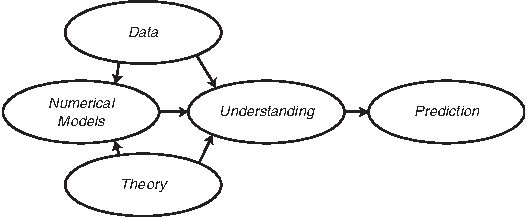
\includegraphics{pics/bigpicture}} 
\footnotesize
Figure 1.1 Data, numerical models, and \rule{0mm}{4ex}theory are
all necessary to understand the ocean. Eventually, an
understanding of the ocean-atmosphere-land system will lead to
predictions of future states of the system.

\label{fig:bigpicture}
\vspace{-1ex}
\end{figure}

The combination of theory, observations, and computer
models\index{numerical models} is relatively new. Four decades of
exponential growth in computing power has made available desktop
computers capable of simulating important physical processes and
oceanic dynamics.
\begin{quote} \small
All of us who are involved in the sciences know that the computer has
become an essential tool for research \dots scientific computation has
reached the point where it is on a par with laboratory experiment and
mathematical theory as a tool for research in science and
engineering---Langer (1999).
\end{quote}

The combination of theory, observations, and computer models also
implies a new way of doing oceanography\index{oceanography!new methods of}.
In the past, an oceanographer would devise a theory, collect
data to test the theory, and publish the results. Now, the tasks have
become so specialized that few can do it all. Few excel in theory,
collecting data, and numerical simulations. Instead, the work is done
more and more by teams of scientists and engineers.

\section{Further Reading}
If you know little about the ocean and oceanography, I suggest you
begin by reading MacLeish's (1989) book \textit{The Gulf
  Stream\index{Gulf Stream}: Encounters With the Blue God}, especially
his Chapter 4 on ``Reading the ocean.'' In my opinion, it is the best
overall, non-technical, description of how oceanographers came to
understand the ocean.

You may also benefit from reading pertinent chapters from any
introductory oceanographic textbook. Those by Gross, Pinet, or Segar
are especially useful. The three texts produced by the Open University
provide a slightly more advanced treatment.

\begin{description}
\item[Gross,] M. Grant and Elizabeth Gross (1996)
  \textit{Oceanography---A View of Earth.} 7th edition. Prentice Hall.
\vspace{-0.8ex}
\item[MacLeish,] William (1989) \textit{The Gulf Stream: Encounters
  With the Blue God.} Houghton Mifflin Company.
\vspace{-0.8ex}
\item[Pinet,] Paul R. (2006) \textit{Invitation to Oceanography.} 4nd
  edition. Jones and Bartlett Publishers.
\vspace{-0.8ex}
\item[Open University] (2001) \textit{Ocean Circulation.} 2nd
  edition. Pergamon Press.
\vspace{-0.8ex}
\item[Open University] (1995) \textit{Seawater: Its Composition,
  Properties and Behavior.} 2nd edition. Pergamon Press.
\vspace{-0.8ex}
\item[Open University] (1989) \textit{Waves, Tides and Shallow-Water
  Processes.} Pergamon Press.
\vspace{-0.8ex}
\item[Segar,] Douglas A. (2007) \textit{Introduction to Ocean
  Sciences.} 2nd edition. W. W. Norton.
\end{description}

\chapter{The Historical Setting} 

Our knowledge of oceanic currents, winds, waves, and tides goes back
thousands of years. Polynesian navigators traded over long distances
in the Pacific as early as 4000 \textsc{bc} (Service, 1996). Pytheas
explored the Atlantic from Italy to Norway in 325 \textsc{bc}. Arabic
traders used their knowledge of the reversing winds and currents in
the Indian Ocean to establish trade routes to China in the Middle Ages
and later to Zanzibar on the African coast. And, the connection
between tides and the sun\index{sun} and moon\index{moon} was
described in the Samaveda of the Indian Vedic period extending from
2000 to 1400 \textsc{bc} (Pugh, 1987).  Those oceanographers who tend
to accept as true only that which has been measured by instruments,
have much to learn from those who earned their living on the ocean.

Modern European knowledge of the ocean began with voyages of discovery
by Bartholomew Dias (1487--1488), Christopher Columbus (1492--1494),
Vasco da Gama (1497--1499), Ferdinand Magellan (1519--1522), and many
others. They laid the foundation for global trade routes stretching
from Spain to the Philippines in the early 16th century. The routes
were based on a good working knowledge of trade winds, the westerlies,
and western boundary currents in the Atlantic and Pacific (Couper,
1983: 192--193).

The early European explorers were soon followed by scientific voyages
of discovery led by (among many others) James Cook (1728--1779) on the
\textit{Endeavour}, \textit{Resolution}, and \textit{Adventure},
Charles Darwin (1809--1882) on the \textit{Beagle}, Sir James Clark
Ross and Sir John Ross who surveyed the Arctic and Antarctic regions
from the \textit{Victory}, the \textit{Isabella}, and the
\textit{Erebus}, and Edward Forbes (1815--1854) who studied the
vertical distribution of life in the ocean. Others collected oceanic
observations and produced useful charts, including Edmond Halley who
charted the trade winds and monsoons and Benjamin Franklin who charted
the Gulf Stream\index{Gulf Stream!mapped by Benjamin Franklin}.

Slow ships of the 19th and 20th centuries gave way to satellites,
drifters, and autonomous instruments toward the end of the 20th
century. Satellites now observe the ocean, air, and land. Thousands of
drifters observe the upper two kilometers of the ocean. Data from
these systems, when fed into numerical models allows the study of
earth as a system.  For the first time, we can study how biological,
chemical, and physical systems interact to influence our environment.

\section{Definitions}
The long history of the study of the ocean has led to the development
of various, specialized disciplines each with its own interests and
vocabulary. The more important disciplines include:

\textit{Oceanography} is \index{oceanography|textbf}the study of the
ocean, with emphasis on its character as an environment. The goal is
to obtain a description sufficiently quantitative to be used for
predicting the future with some certainty.

\textit{Geophysics} is \index{geophysics|textbf}the study of the
physics of the earth.

\textit{Physical Oceanography} is \index{physical oceanography|textbf}the
study of physical properties and dynamics of
the ocean. The primary interests are the interaction of the ocean with
the atmosphere, the oceanic heat budget, water mass formation,
currents, and coastal dynamics. Physical Oceanography is considered by
many to be a subdiscipline of geophysics.

\textit{Geophysical Fluid Dynamics} is
\index{geophysical fluid dynamics|textbf}the study of the dynamics of
fluid motion on scales influenced by the rotation of the
earth. Meteorology and oceanography use geophysical fluid dynamics to
calculate planetary flow fields.

\textit{Hydrography} is \index{hydrography|textbf}the preparation of
nautical charts, including charts of ocean depths, currents, internal
density field of the ocean, and tides.

\textit{Earth-system Science} is
\index{earth-system science|textbf}the study of earth as a single
system comprising many interacting subsystems including the ocean,
atmosphere, cryosphere, and biosphere, and changes in these systems
due to human activity.

\begin{figure}[t!]
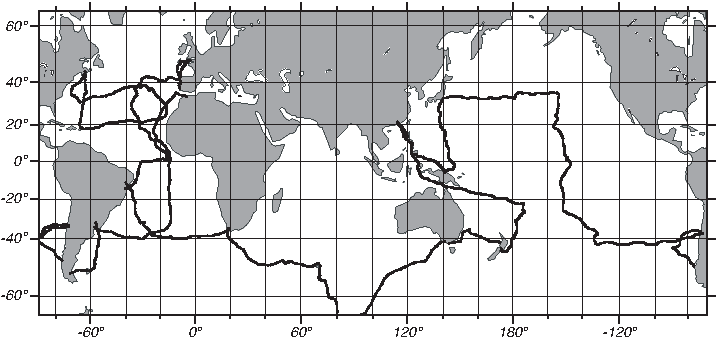
\includegraphics{pics/Fig2-1}
\centering
\footnotesize
Figure 2.1 Example from the era\rule{0pt}{3ex} of deep-sea
exploration: Track of H.M.S. \textit{Challenger}\\ during the British
Challenger Expedition 1872--1876. After Wust (1964).

\label{fig:Fig2-1}
\vspace{-3ex}
\end{figure}


\begin{figure}[t!]
\makebox[121mm] [c] {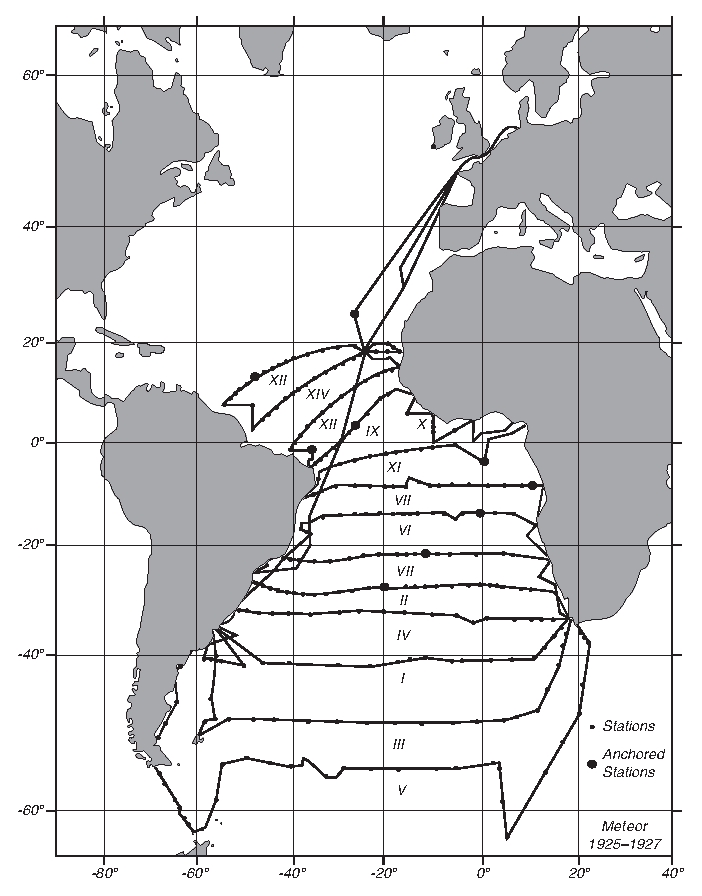
\includegraphics{pics/Fig2-2}}
\centering
\footnotesize
Figure 2.2 Example of a survey from the era of national\rule{0pt}{3ex}
systematic surveys. Track of the R/V \textit{Meteor} during the German
Meteor Expedition. Redrawn from Wust (1964).

\label{fig:Fig2-2}
\vspace{-3ex}
\end{figure}
\section{Eras of Oceanographic Exploration}
The exploration \index{oceanography!eras of exploration|(}of the sea
can be divided, somewhat arbitrarily, into various eras (Wust,
1964). I have extended his divisions through the end of the 20th
century.
\begin{enumerate}
\vitem Era of Surface Oceanography: Earliest times to 1873. The era is
characterized by systematic collection of mariners' observations of
winds, currents, waves, temperature, and other phenomena observable
from the deck of sailing ships. Notable examples include Halley's
charts of the trade winds, Franklin's map of the Gulf
Stream\index{Gulf Stream!mapped by Benjamin Franklin}, and Matthew
Fontaine Maury's \textit{Physical Geography of the Sea}.

\vitem Era of Deep-Sea Exploration: 1873--1914.  Characterized by a
few, wide-ranging oceanographic expeditions to survey surface and
subsurface conditions, especially near colonial claims. The major
example is the \textit{Challenger} Expedition (figure 2.1), but also
the \textit{Gazelle} and \textit{Fram} Expeditions.  \vitem Era of
National Systematic Surveys: 1925--1940.  Characterized by detailed
surveys of colonial areas. Examples include \textit{Meteor} surveys of
the Atlantic (figure 2.2), and the \textit{Discovery} Expeditions.

\vitem Era of New Methods: 1947--1956.  Characterized by long surveys
using new instruments (figure 2.3). Examples include seismic surveys
of the Atlantic by \textit{Vema} leading to Heezen's maps of the sea
floor.

\begin{figure}[t!]
\makebox[121 mm] [c] {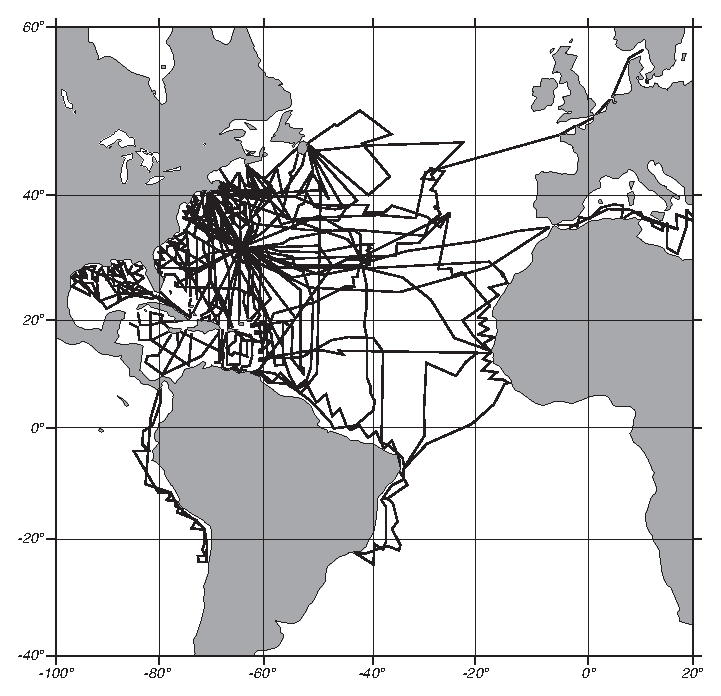
\includegraphics{pics/Fig2-3}}
\centering
\footnotesize
Figure 2.3 Example from the era of new \rule{0pt}{4ex}methods. The
cruises of the R/V \textit{Atlantis} out of Woods Hole Oceanographic
Institution. After Wust (1964).

\label{fig:Fig2-3}
\vspace{-3ex}
\end{figure}

\vitem Era of International Cooperation: 1957--1978. Characterized by
multinational surveys of ocean and studies of oceanic
processes. Examples include the Atlantic Polar Front Program, the
\textsc{norpac} cruises, the International Geophysical Year cruises,
and the International Decade of Ocean Exploration (figure 2.4).
Multiship studies of oceanic processes include \textsc{mode},
\textsc{polymode}, \textsc{norpax}, and \textsc{jasin} experiments.

\begin{figure}[t!]
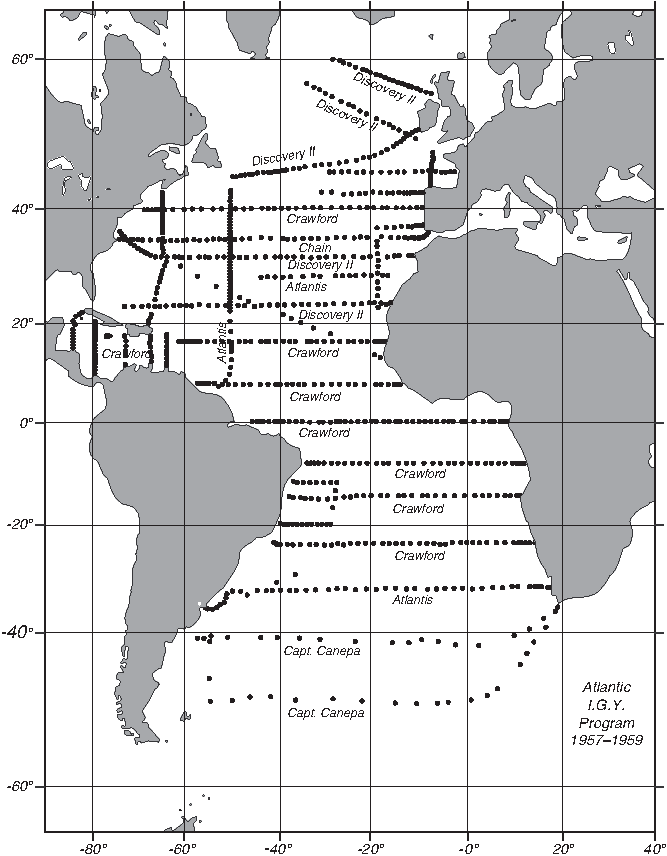
\includegraphics{pics/Fig2-4}
\centering
\footnotesize
Figure 2.4 Example from the era of international cooperation
\rule{0pt}{3ex}. Sections measured by the International Geophysical
Year Atlantic Program 1957-1959. After Wust (1964).

\label{fig:Fig2-4}
\vspace{-3ex}
\end{figure}

\vitem Era of Satellites: 1978--1995. Characterized by global surveys
of oceanic processes from space. Examples include Seasat,
\textsc{noaa} 6--10, \textsc{nimbus}--7, Geosat\index{Geosat},
Topex/\-Poseidon\index{Topex/Poseidon}, and \textsc{ers}--1 \&
2\index{ERS satellites}.

\vitem Era of Earth System Science: 1995-- Characterized by global
studies of the interaction of biological, chemical, and physical
processes in the ocean and atmosphere and on land using \textit{in
  situ} \index{in situ|textbf} (which means from measurements made in
the water) and space data in numerical models. Oceanic examples
include the World Ocean Circulation Experiment
(\textsc{woce})\index{World Ocean Circulation Experiment} (figure 2.5)
and Topex/Poseidon (figure 2.6), the Joint Global Ocean Flux Study
\index{oceanography!eras of exploration|)} (\textsc{jgofs}), the
Global Ocean Data Assimilation Experiment (\textsc {godae}), and the
SeaWiFS, Aqua, and Terra satellites.
\end{enumerate}

\begin{figure}[t!]
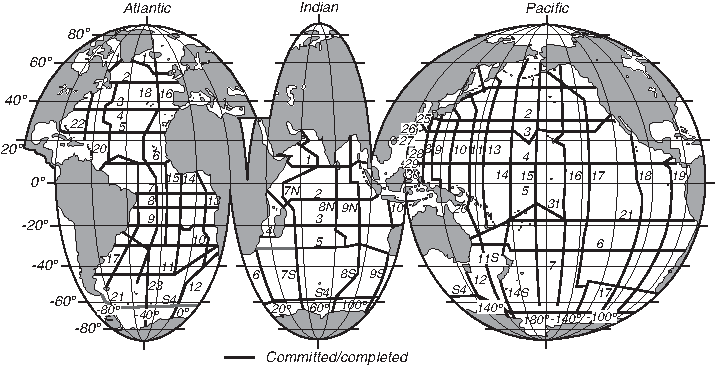
\includegraphics{pics/wocesurvey}
\centering
\footnotesize
Figure 2.5 World Ocean\index{World Ocean Circulation Experiment}
Circulation Experiment:\rule{0pt}{4ex} Tracks of research ships making
a one-time global survey of the ocean of the world. From World Ocean
Circulation Experiment.

\label{fig:wocesurvey}
\vspace{-3ex}
\end{figure}

\begin{figure}[b!]
\vspace{-1ex}
\makebox[121mm][c]{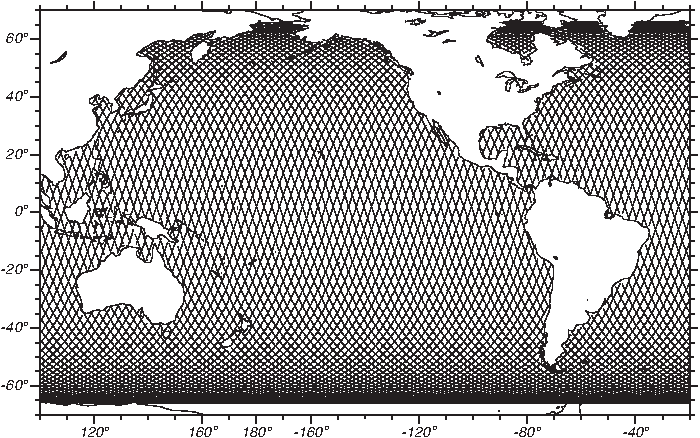
\includegraphics{pics/Fig2-6}}
\centering
\footnotesize
Figure 2.6 Example \rule{0mm}{3ex}from the era of satellites.
Topex/Poseidon\index{Topex/Poseidon!ground tracks} tracks in the
Pacific\\Ocean during a 10-day repeat of the orbit. From
Topex/Poseidon Project.

\label{fig:Fig2-6}
%\vspace{-3ex}
\end{figure}

\vspace{-1ex}
\section{Milestones in the Understanding of the Ocean}
What have all these programs and expeditions taught us about the
ocean?  Let's look at some milestones in our ever increasing
understanding of the ocean beginning with the first scientific
investigations of the 17th century.  Initially progress was
slow. First came very simple observations of far reaching importance
by scientists who probably did not consider themselves oceanographers,
if the term even existed. Later came more detailed descriptions and
oceanographic experiments by scientists who specialized in the study
of the ocean.
\vspace{-1.0ex}
\begin{description}
\item[1685] Edmond Halley, investigating \index{ocean!milestones in
  understanding|(}the oceanic wind systems and currents, published
  ``An Historical Account of the Trade Winds, and Monsoons, observable
  in the Seas between and near the Tropicks, with an attempt to assign
  the Physical cause of the said Winds'' \textit{Philosophical
    Transactions}. \vspace{-1.0ex}

\item[1735] George Hadley published his theory for the trade winds
  based on conservation of angular momentum in ``Concerning the Cause
  of the General Trade-Winds'' \textit{Philosophical Transactions},
  39: 58-62. \vspace{-1.0ex}

\item[1751] Henri Ellis made the first deep soundings of temperature
  in the tropics, finding cold water below a warm surface layer,
  indicating the water came from the polar regions. \vspace{-1.0ex}

\item[1769] Benjamin Franklin, as postmaster, made the first map of
  the Gulf Stream\index{Gulf Stream!mapped by Benjamin Franklin} using
  information from mail ships sailing between New England and England
  collected by his cousin Timothy Folger (figure 2.7).

\begin{figure}[t!]
\makebox[121mm][c]{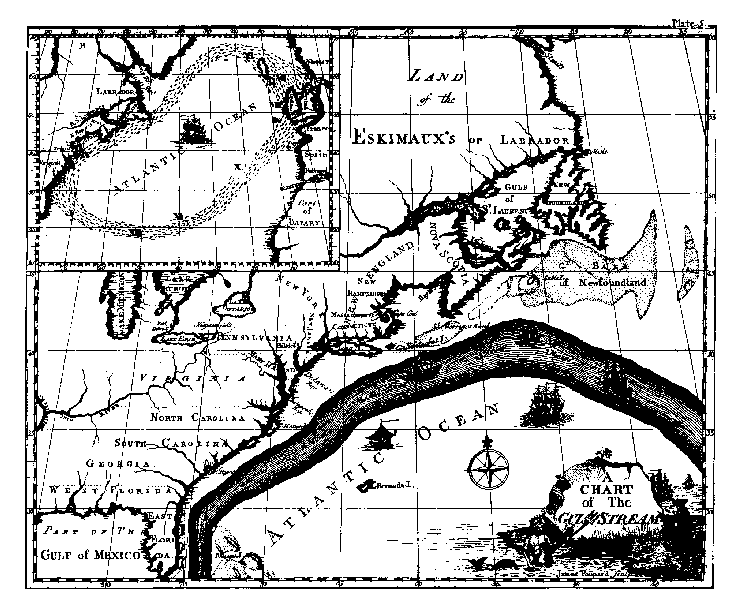
\includegraphics{pics/Fig2-7}}
\centering
\footnotesize
Figure 2.7 The 1786 version of Franklin-Folger map \rule{0mm}{3ex}of
the Gulf Stream\index{Gulf Stream!Franklin-Folger map of}.
\label{fig:Fig2-7}
\vspace{-2ex}
\end{figure}

\vspace{-1.0ex} 
\item[1775] Laplace's published his theory of
  tides. \vspace{-1.0ex} \item[1800] Count Rumford proposed a
  meridional\index{circulation!meridional overturning} circulation of
  the ocean with water sinking near the poles and rising near the
  Equator. \vspace{-1.0ex}

\item[1847] Matthew Fontaine Maury published his first chart of winds
  and currents based on ships logs. Maury established the practice of
  international exchange of environmental data, trading logbooks for
  maps and charts derived from the data. \vspace{-1.0ex}

\item[1872--1876] Challenger Expedition marks the beginning of the
  systematic study of the biology, chemistry, and physics of the ocean
  of the world. \vspace{-1.0ex}

\item[1885] Pillsbury made direct measurements of the Florida Current
  using current meters deployed from a ship moored in the
  stream. \vspace{-1.0ex}

\item[1903] Founding of the Marine Biological Laboratory of the
  University of California. It later became the Scripps Institution of
  Oceanography.
\vspace{-1.0ex}

\item[1910--1913] Vilhelm Bjerknes published \textit{Dynamic
  Meteorology and Hydrography} which laid the foundation of
  geophysical fluid dynamics. In it he developed the idea of fronts,
  the dynamic meter, geostrophic\index{geostrophic currents} flow,
  air-sea interaction, and cyclones. \vspace{-1.0ex}

\item[1930] Founding of the Woods Hole Oceanographic Institution.
\vspace{-1.0ex} 

\item[1942] Publication of \textit{The ocean} by Sverdrup, Johnson,
  and Fleming, a comprehensive survey of oceanographic knowledge up to
  that time. \vspace{-1.0ex}

\item[Post WW 2] The need to detect submarines led the navies of the
  world to greatly expand their studies of the sea. This led to the
  founding of oceanography departments at state universities,
  including Oregon State, Texas A\&M University, University of Miami,
  and University of Rhode Island, and the founding of national ocean
  laboratories such as the various Institutes of Oceanographic
  Science. \vspace{-1.0ex}

\item[1947--1950] Sverdrup, Stommel, and Munk publish their theories
  of the wind-driven circulation of the ocean. Together the three
  papers lay the foundation for our understanding of the ocean's
  circulation. \vspace{-1.0ex}

\item[1949] Start of California Cooperative Fisheries Investigation of
  the California Current. The most complete study ever undertaken of a
  coastal current. \vspace{-1.0ex}

\item[1952] Cromwell and Montgomery rediscover the Equatorial
  Undercurrent in the Pacific. \vspace{-1.0ex}

\item[1955] Bruce Hamon and Neil Brown develop the CTD\index{CTD} for
  measuring conductivity and temperature as a function of depth in the
  ocean.
\vspace{-1.0ex} 

\item[1958] Stommel publishes his theory for the deep circulation of
  the ocean.
\vspace{-1.0ex}

\item[1963] Sippican Corporation (Tim Francis, William Van Allen
  Clark, Graham Campbell, and Sam Francis) invents the Expendable
  BathyThermograph \textsc{xbt} now perhaps the most widely used
  oceanographic instrument deployed from ships.
\vspace{-1.0ex}

\item[1969] Kirk Bryan and Michael Cox develop the first numerical
  model of the oceanic circulation.
\vspace{-1.0ex} 

\item[1978] \textsc{nasa} launches the first oceanographic satellite,
  Seasat. The project developed techniques used by generations of
  remotes sensing satellites.
\vspace{-1.0ex}

\item[1979--1981] Terry Joyce, Rob Pinkel, Lloyd Regier, F. Rowe and
  J. W. Young develop techniques leading to the acoustic-doppler
  current profiler for measuring ocean-surface currents from moving
  ships, an instrument widely used in oceanography.
\vspace{-1.0ex}

\item[1988] \textsc{nasa} Earth System Science Committee headed by
  Francis Bretherton outlines how all earth systems are
  interconnected, thus breaking down the barriers separating
  traditional sciences of astrophysics, ecology, geology, meteorology,
  and oceanography.

\item[1991] Wally Broecker proposes that changes in the deep
  circulation of the ocean modulate the ice ages, and that the deep
  circulation in the Atlantic could collapse, plunging the northern
  hemisphere into a new ice age.\index{ocean!milestones in
    understanding|)}
\vspace{-1.0ex}

\item[1992] Russ Davis and Doug Webb invent the autonomous, pop-up
  drifter that continuously measures currents at depths to 2 km.
\vspace{-1.0ex} 

\item[1992] \textsc{nasa} and \textsc{cnes} develop and launch
  Topex/Poseidon\index{Topex/Poseidon}, a satellite that maps ocean
  surface currents, waves, and tides every ten days, revolutionizing
  our understanding of ocean dynamics and tides.

\item[1993] Topex/Poseidon science-team members publish first accurate
  global maps of the tides\index{tides}.

\end{description}
\vspace{-1.0ex}
More information on the history of physical oceanography can be found
in Appendix A of W.S. von Arx (1962): \textit{An Introduction to
  Physical Oceanography}.

Data collected from the centuries of oceanic expeditions have been
used to describe the ocean. Most of the work went toward describing
the steady state of the ocean, its currents from top to bottom, and
its interaction with the atmosphere. The basic description was mostly
complete by the early 1970s. Figure 2.8 shows an example from that
time, the surface circulation of the ocean. More recent work has
sought to document the variability of oceanic processes, to provide a
description of the ocean sufficient to predict annual and interannual
variability, and to understand the role of the ocean in global
processes.

\begin{figure}[t!]
\makebox[121mm][c]{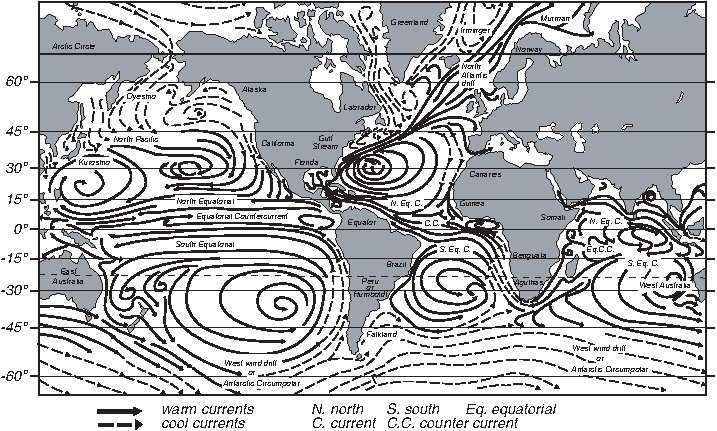
\includegraphics{pics/Fig2-8}}
\centering
\footnotesize
Figure 2.8 The time-averaged, surface circulation \rule{0mm}{3ex}of
the ocean during northern hemisphere winter deduced from a century of
oceanographic expeditions. After Tolmazin (1985: 16).

\label{fig:Fig2-8}
\vspace{-3ex}
\end{figure}

\section{Evolution of some Theoretical Ideas}
A theoretical understanding of oceanic processes is based on classical
physics coupled with an evolving understanding of chaotic systems in
mathematics and the application to the theory of
turbulence\index{turbulence!theory of}. The dates given below are
approximate.
\vspace{-1.0ex}
\begin{description}
\item[19th Century] Development of analytic hydrodynamics. Lamb's
  \textit{Hydrodynamics} is the pinnacle of this work. Bjerknes
  develops geostrophic\index{geostrophic currents} method widely used
  in meteorology and oceanography.
\vspace{-1.0ex}
\item[1925--40] Development of theories for turbulence based on
  aerodynamics and mixing-length\index{mixing-length theory}
  ideas. Work of Prandtl and von Karman.
\vspace{-1.0ex}
\item[1940--1970] Refinement of theories for
  turbulence\index{turbulence!theory of} based on statistical
  correlations and the idea of isotropic homogeneous turbulence. Books
  by Batchelor (1967), Hinze (1975), and others.
\vspace{-1.0ex}
\item[1970--] Numerical investigations of turbulent geophysical fluid
  dynamics based on high-speed digital computers.
\vspace{-1.0ex}
\item[1985--] Mechanics of chaotic processes. The application to
  hydrodynamics is just beginning. Most motion in the atmosphere and
  ocean may be inherently unpredictable.
\end{description}

\section{The Role of Observations in Oceanography}
\index{observations}The brief tour of theoretical ideas suggests that
observations are essential for understanding the ocean. The theory
describing a convecting, wind-forced, tur\-bulent fluid in a rotating
coordinate system has never been sufficiently well known that
important features of the oceanic circulation could be predicted
before they were observed. In almost all cases, oceanographers resort
to observations to understand oceanic processes.

At first glance, we might think that the numerous expeditions mounted
since 1873 would give a good description of the ocean. The results are
indeed impressive. Hundreds of expeditions have extended into all
ocean. Yet, much of the ocean is poorly explored.

By the year 2000, most areas of the ocean will have been sampled from
top to bottom only once. Some areas, such as the Atlantic, will have
been sparsely sampled three times: during the International
Geophysical Year in 1959, during the Geochemical Sections cruises in
the early 1970s, and during the World Ocean Circulation
Experiment\index{World Ocean Circulation Experiment} from 1991 to
1996. All areas will be vastly under sampled. This is the sampling
problem\index{sampling error} (See box on next page). Our samples of
the ocean are insufficient to describe the ocean well enough to
predict its variability and its response to changing
forcing. \textit{Lack of sufficient samples is the largest source of
  error in our understanding of the ocean.}

The lack of observations has led to a very important and widespread
conceptual error:
\begin{quote} \small
\textit{``The absence of evidence was taken as evidence of absence.''}
The great difficulty of observing the ocean meant that when a
phenomenon was not observed, it was assumed it was not present. The
more one is able to observe the ocean, the more the complexity and
subtlety that appears---Wunsch (2002a).
\end{quote}
As a result, our understanding of the ocean is often too simple to be
correct.

\begin{figure} [t!]
\fbox{\parbox{12cm}{
\centering
\vspace{-0.5 em}
\section*{Sampling Error}
\begin{minipage}{11.5cm}
\vspace{0.5 em} \hspace*{1 em}Sampling error \index{sampling
  error|textbf}is the largest source of error in the geosciences. It
is caused by a set of samples not representing the population of the
variable being measured. A population is the set of all possible
measurements, and a sample is the sampled subset of the population. We
assume each measurement is perfectly accurate.

\hspace*{1 em}To determine if your measurement has a sampling error,
you must first completely specify the problem you wish to study. This
defines the population. Then, you must determine if the samples
represent the population.  Both steps are necessary.

\hspace*{1 em}Suppose your problem is to measure the annual-mean
sea-surface temperature of the ocean to determine if global warming is
occurring. For this problem, the population is the set of all possible
measurements of surface temperature, in all regions in all months. If
the sample mean is to equal the true mean, the samples must be
uniformly distributed throughout the year and over all the area of the
ocean, and sufficiently dense to include all important variability in
time and space. This is impossible. Ships avoid stormy regions such as
high latitudes in winter, so ship samples tend not to represent the
population of surface temperatures. Satellites may not sample
uniformly throughout the daily cycle, and they may not observe
temperature at high latitudes in winter because of persistent clouds,
although they tend to sample uniformly in space and throughout the
year in most regions. If daily variability is small, the satellite
samples will be more representative of the population than the ship
samples.

\hspace*{1 em}From the above, it should be clear that oceanic samples
rarely represent the population we wish to study. We always have
sampling errors.

\hspace*{1 em}In defining sampling error, we must clearly distinguish
between instrument errors and sampling errors. Instrument errors are
due to the inaccuracy of the instrument. Sampling errors are due to a
failure to make a measurement. Consider the example above: the
determination of mean sea-surface temperature. If the measurements are
made by thermometers on ships, each measurement has a small error
because thermometers are not perfect. This is an instrument error. If
the ships avoids high latitudes in winter, the absence of measurements
at high latitude in winter is a sampling error.

\hspace*{1 em}Meteorologists designing the Tropical Rainfall Mapping
Mission have been investigating the sampling error in measurements of
rain. Their results are general and may be applied to other
variables. For a general description of the problem see North \&
Nakamoto (1989).
\vspace{0.7ex}
\end{minipage}
}}
\vspace{-4ex}
\end{figure}

\paragraph{Selecting Oceanic Data Sets}
\index{data sets}Much of the existing oceanic data have been organized
into large data sets. For example, satellite data are processed and
distributed by groups working with \textsc{nasa}.  Data from ships
have been collected and organized by other groups.  Oceanographers now
rely more and more on such collections of data produced by others.

The use of data produced by others introduces problems: i) How
accurate are the data in the set? ii) What are the limitations of the
data set? And, iii) How does the set compare with other similar sets?
Anyone who uses public or private data sets is wise to obtain answers
to such questions.

If you plan to use data from others, here are some guidelines.

\begin{enumerate}
\vitem \textit{Use well documented data sets}. \index{data sets!what
  makes good data?|(}Does the documentation completely describe the
sources of the original measurements, all steps used to process the
data, and all criteria used to exclude data? Does the data set include
version numbers to identify changes to the set?

\vitem \textit{Use validated data}. \index{data!validated|textbf}Has
accuracy\index{accuracy} of data been well documented? Was accuracy
determined by comparing with different measurements of the same
variable? Was validation global or regional?

\vitem \textit{Use sets that have been used by others and referenced
  in scientific papers}. Some data sets are widely used for good
reason.  Those who produced the sets used them in their own published
work and others trust the data.

\vitem \textit{Conversely, don't use a data set just because it is
  handy}. Can you document the source of the set? For example, many
versions of the digital, 5-minute maps of the sea floor are widely
available. Some date back to the first sets produced by the
U.S. Defense Mapping Agency, others are from the \textsc{etopo-5}
set. Don't rely on a colleague's statement about the source. Find the
documentation. If it is missing, find another data set.\index{data
  sets!what makes good data?|)}
\end{enumerate}

\paragraph{Designing Oceanic Experiments}
\index{oceanic experiments}Observations are exceedingly important for
ocean\-ography, yet observations are expensive because ship time and
satellites are expensive. As a result, oceanographic experiments must
be carefully planned. While the design of experiments may not fit well
within an historical chapter, perhaps the topic merits a few brief
comments because it is seldom mentioned in oceanographic textbooks,
although it is prominently described in texts for other scientific
fields. The design of experiments is particularly important because
poorly planned experiments lead to ambiguous results, they may measure
the wrong variables, or they may produce completely useless data.

The first and most important aspect of the design of any experiment is
to determine \textit{why} you wish to make a measurement before
deciding how you will make the measurement or what you will measure.
\begin{enumerate}
\vitem What is the purpose of the observations? Do you wish to test
hypotheses or describe processes?

\vitem What accuracy\index{accuracy} is required of the observation?

\vitem What resolution in time and space is required? What is the
duration of measurements?
\end{enumerate}
Consider, for example, how the purpose of the measurement changes how
you might measure salinity or temperature as a function of depth:
\begin{enumerate}
\vitem If the purpose is to describe water masses in an ocean basin,
then measurements with 20--50 m vertical spacing and 50--300 km
horizontal spacing, repeated once per 20--50 years in deep water are
required.

\vitem If the purpose is to describe vertical
mixing\index{mixing!vertical} in the open equatorial Pacific, then
0.5--1.0 mm vertical spacing and 50--1000 km spacing between locations
repeated once per hour for many days may be required.
\end{enumerate}

\paragraph{Accuracy, Precision, and Linearity}
While we are on the topic of experiments, now is a good time to
introduce three concepts needed throughout the book when we discuss
experiments: precision, accuracy, and linearity of a measurement.

\textit{Accuracy} \index{accuracy|textbf}is the difference between the
measured value and the true value.

\textit{Precision} \index{precision|textbf}is the difference among
repeated measurements.

The distinction between accuracy and precision is usually illustrated
by the simple example of firing a rifle at a target. Accuracy is the
average distance from the center of the target to the hits on the
target. Precision is the average distance between the hits. Thus, ten
rifle shots could be clustered within a circle 10 cm in diameter with
the center of the cluster located 20 cm from the center of the
target. The accuracy is then 20 cm, and the precision is roughly 5 cm.

\textit{Linearity} \index{linearity|textbf}requires that the output of
an instrument be a linear function of the input. Nonlinear devices
rectify variability to a constant value. So a non-linear response
leads to wrong mean values. Non-linearity can be as important as
accuracy.  For example, let
\begin{align}
Output &= Input + 0.1(Input)^2 \notag \\
Input &= a \sin \omega t \notag
\end{align}
then
\begin{align}
Output &= a \sin \omega t + 0.1\,(a \sin \omega t)^2 \notag \\
Output &= Input + \frac{0.1}{2} a^2 - \frac{0.1}{2} a^2 \cos 2\omega t
\notag
\end{align}
Note that the mean value of the input is zero, yet the output of this
non-linear instrument has a mean value of \(0.05 a^2\) plus an equally
large term at twice the input frequency. In general, if \textit{input}
has frequencies \(\omega_1\) and \(\omega_2\), then \textit{output} of
a non-linear instrument has frequencies \(\omega_1 \pm \omega_2\).
Linearity of an instrument is especially important when
the instrument must measure the mean value of a turbulent
variable. For example, we require linear current meters when measuring
currents near the sea surface where wind and waves produce a large
variability in the current.

\paragraph{Sensitivity to other variables of interest.}
Errors may be correlated with other variables of the problem. For
example, measurements of conductivity are sensitive to
temperature. So, errors in the measurement of temperature in
salinometers leads to errors in the measured values of conductivity or
salinity.

\section{Important Concepts}
From the above, I hope you have learned:
\begin{enumerate}
\vitem The ocean is not well known. What we know is based on data
collected from only a little more than a century of oceanographic
expeditions supplemented with satellite data collected since 1978.

\vitem The basic description of the ocean is sufficient for describing
the time-averaged mean circulation of the ocean, and recent work is
beginning to describe the variability.

\vitem Observations are essential for understanding the ocean. Few
processes have been predicted from theory before they were observed.

\vitem Lack of observations has led to conceptual pictures of oceanic
processes that are often too simplified and often misleading.

\vitem Oceanographers rely more and more on large data sets produced
by others.  The sets have errors and limitations which you must
understand before using them.

\vitem The planning of experiments is at least as important as
conducting the experiment.

\vitem Sampling errors arise when the observations, the samples, are
not representative of the process being studied. Sampling errors are
the largest source of error in oceanography.

\vitem Almost all our observations of the ocean now come from
satellites, drifters, and autonomous instruments. Fewer and fewer
observations come from ships at sea.
\end{enumerate}

\chapter{The Physical Setting}
\addtocounter{figure}{1}

Earth \index{earth!radii of}is an oblate ellipsoid, an ellipse rotated
about its minor axis, with an equatorial radius of $R_e = 6,378.1349$
km (West, 1982) slightly greater than the polar radius of $R_p =
6,356.7497$ km. The small equatorial bulge is due to earth's rotation.

Distances on earth are measured in many different units, the most
common are degrees of latitude or longitude, meters, miles, and
nautical miles.  \textit{Latitude}\index{latitude|textbf} is the angle
between the local vertical and the equatorial plane. A meridian is the
intersection at earth's surface of a plane perpendicular to the
equatorial plane and passing through earth's axis of rotation.
\textit{Longitude}\index{longitude|textbf} is the angle between the
standard meridian and any other meridian, where the standard meridian
is the one that passes through a point at the Royal Observatory at
Greenwich, England.  Thus longitude is measured east or west of
Greenwich.

A degree of latitude is not the same length as a degree of longitude
except at the equator. Latitude is measured along great circles with
radius $R$, where $R$ is the mean radius of earth. Longitude is
measured along circles with radius $R \cos \varphi$, where $\varphi$
is latitude. Thus $1^{\circ}$ latitude $ = 111$ km, and $1^{\circ}$
longitude $= 111 \cos \varphi$ km.

Because distance in degrees of longitude is not constant,
oceanographers measure distance on maps using degrees of latitude.

Nautical miles and meters are connected historically to the size of
earth. Gabriel Mouton proposed in 1670 a decimal system of measurement
based on the length of an arc that is one minute of a great circle of
earth.  This eventually became the nautical mile. Mouton's decimal
system eventually became the metric system based on a different unit
of length, the meter, which was originally intended to be one
ten-millionth the distance from the Equator to the pole along the
Paris meridian. Although the tie between nautical miles, meters, and
earth's radius was soon abandoned because it was not practical, the
approximations are very good. For example, earth's polar circumference
is approximately 40,008 km. Therefore one ten-millionth of a quadrant
is 1.0002 m. Similarly, a nautical mile should be 1.8522 km, which is
very close to the official definition of the\index{nautical
  mile|textbf}\index{international nautical mile|textbf}
\textit{international nautical mile}: 1 nm $\equiv$ 1.8520 km.

\section{Ocean and Seas}
There is only one ocean. It is divided into three named parts by
international agreement: the Atlantic, Pacific, and Indian
ocean\index{ocean!defined} (International Hydrographic Bureau,
1953)\index{International Hydrographic Bureau}. Seas, which are part
of the ocean, are defined in several ways. I consider two.

\begin{figure}[t!]
\makebox[121 mm] [c]{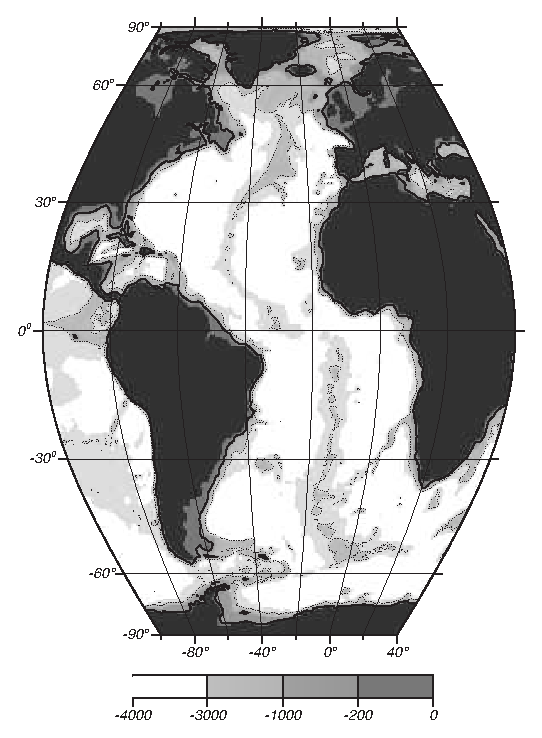
\includegraphics{pics/atlantic}} \footnotesize
\centering Figure 3.1 The Atlantic Ocean viewed with an Eckert
VI\rule{0mm}{3ex} equal-area projection. Depths, in meters, are
from the \textsc{etopo} 30$'$ data set. The 200 m contour outlines
continental shelves.

\label{fig:atlantic}
\vspace{-4ex}
\end{figure}

\textbf{The Atlantic Ocean} \index{ocean!Atlantic Ocean}extends
northward from Antarctica and includes all of the Arctic Sea, the
European Mediterranean, and the American Mediterranean more commonly
known as the Caribbean sea (figure 3.1). The boundary between the
Atlantic and Indian Ocean is the meridian of Cape Agulhas (20\degrees
E). The boundary between the Atlantic and Pacific is the line forming
the shortest distance from Cape Horn to the South Shetland Islands. In
the north, the Arctic Sea is part of the Atlantic Ocean, and the
Bering Strait is the boundary between the Atlantic and Pacific.

\textbf{The Pacific Ocean} \index{ocean!Pacific Ocean}extends
northward from Antarctica to the Bering Strait (figure 3.2). The
boundary between the Pacific and Indian Ocean follows the line from
the Malay Peninsula through Sumatra, Java, Timor, Australia at Cape
Londonderry, and Tasmania. From Tasmania to Antarctica it is the
meridian of South East Cape on Tasmania 147\degrees E.

\textbf{The Indian Ocean} \index{ocean!Indian Ocean}extends from
Antarctica to the continent of Asia including the Red Sea and Persian
Gulf (figure 3.3). Some authors use the name Southern Ocean to
describe the ocean surrounding Antarctica.

\begin{figure}[t!]
\makebox[121 mm] [c]{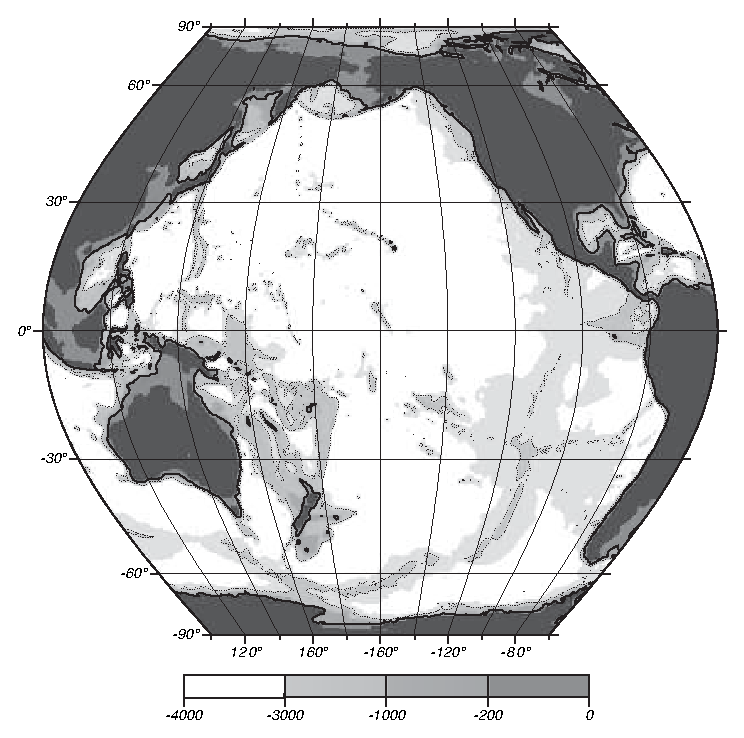
\includegraphics{pics/pacific}}
\centering
\footnotesize
Figure 3.2 The Pacific Ocean viewed with an Eckert VI\rule{0mm}{3ex}
equal-area projection. Depths, in meters, are from the \textsc{etopo}
30$'$ data set. The 200 m contour outlines continental shelves.

\label{fig:pacific}
\vspace{-4ex}
\end{figure}

\begin{figure}[t!]
\makebox[121 mm] [c]{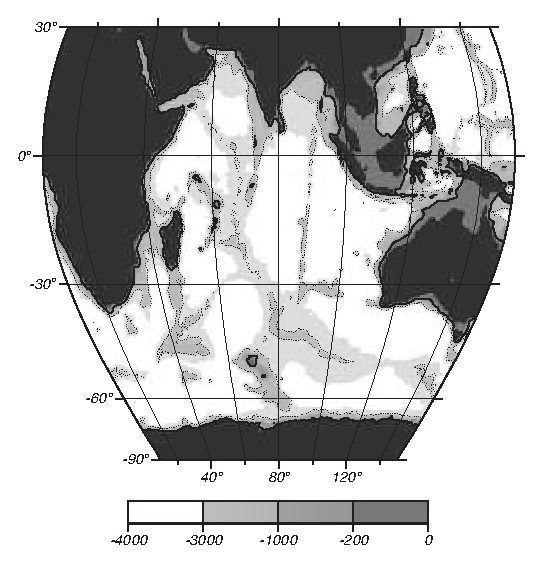
\includegraphics{pics/indian}}
\footnotesize
\centering
Figure 3.3 The Indian Ocean viewed with an Eckert VI\rule{0pt}{3ex}
equal-area projection. Depths, in meters, are from the \textsc{etopo}
30$'$ data set. The 200 m contour outlines continental shelves.

\label{fig:indian}
\vspace{-4ex}
\end{figure}

\textbf{Mediterranean Seas} \index{seas!Mediterranean}are mostly
surrounded by land. By this definition, the Arctic and Caribbean Seas
are both Mediterranean Seas, the Arctic Mediterranean and the
Caribbean Mediterranean.

\textbf{Marginal Seas} \index{seas!marginal}are defined by only an
indentation in the coast. The Arabian Sea and South China Sea are
marginal seas.

\section{Dimensions of the ocean}
\index{ocean!dimensions of}The ocean and seas cover 70.8\% of the
surface of earth, which amounts to 361,254,000 km$^2$. The areas of
the named parts vary considerably (table 3.1).
 \begin{table} [b!]\centering \small
 \vspace{-3ex}
 \begin{tabular*}{65mm}{@{}l @{\extracolsep{\fill}} r@{}}
 \multicolumn{2}{@{}l@{}}{\bfseries Table 3.1 Surface Area of the ocean} $^{\dag }$ \\
 \hline
 \rule{0ex}{2.5ex}Pacific Ocean  & $181.34 \times 10^6 \hbox{ km}^2$        \\
                  Atlantic Ocean   & $ 106.57 \times 10^6 \hbox{ km}^2$        \\
                 Indian Ocean  & $74.12 \times 10^6 \hbox{ km}^2$        \\[0.5ex]
 \hline
 \multicolumn{2}{@{}l@{}}  {\rule{0ex}{2.5ex}$^{\dag }$ From Menard and Smith (1966)}
 \end{tabular*} \\[0.5ex]
% \vspace{-3ex}
 \end{table}

Oceanic dimensions range from around 1500 km for the minimum width of
the Atlantic to more than 13,000 km for the north-south extent of the
Atlantic and the width of the Pacific. Typical depths are only 3--4
km. So horizontal dimensions of ocean basins are 1,000 times greater
than the vertical dimension. A scale model of the Pacific, the size of
an $8.5 \times 11$ in sheet of paper, would have dimensions similar to
the paper: a width of 10,000 km scales to 10 in, and a depth of 3 km
scales to 0.003 in, the typical thickness of a piece of paper.

Because the ocean is so thin, cross-sectional plots of ocean basins
must have a greatly exaggerated vertical scale to be useful. Typical
plots have a vertical scale that is 200 times the horizontal scale
(figure 3.4). This exaggeration distorts our view of the ocean. The
edges of the ocean basins, the continental slopes, are not steep
cliffs as shown in the figure at 41\degrees W and 12\degrees
E. Rather, they are gentle slopes dropping down 1 meter for every 20
meters in the horizontal.

\begin{figure}[t!]
\makebox[121 mm] [c]{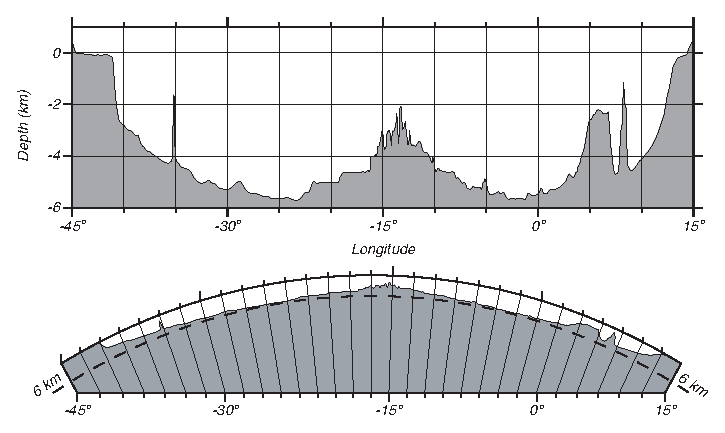
\includegraphics{pics/bathy}}
\footnotesize
Figure 3.4 Cross-section of the south Atlantic\rule{0pt}{3ex} along
25\degrees S showing the continental shelf offshore of South America,
a seamount near 35\degrees W, the mid-Atlantic Ridge near 14\degrees
W, the Walvis Ridge near 6\degrees E, and the narrow continental shelf
off South Africa.  \textbf{Upper} Vertical exaggeration of
180:1. \textbf{Lower} Vertical exaggeration of 30:1. If shown with
true aspect ratio, the plot would be the thickness of the line at the
sea surface in the lower plot.
\label{fig:bathy}
\vspace{-4ex}
\end{figure}

The small ratio of depth to width of the ocean basins is very
important for understanding ocean currents. Vertical velocities must
be much smaller than horizontal velocities. Even over distances of a
few hundred kilometers, the vertical velocity must be less than 1\% of
the horizontal velocity. I will use this information later to simplify
the equations of motion.

The relatively small vertical velocities have great influence on
turbulence\index{turbulence}. Three dimensional turbulence is
fundamentally different than two-dimensional
turbulence\index{turbulence!two dimensional}. In two dimensions,
vortex lines must always be vertical, and there can be little vortex
stretching. In three dimensions, vortex stretching plays a fundamental
role in turbulence.

\section{Sea-Floor Features}
Earth's rocky surface is divided into two types: oceanic, with a thin
dense crust about 10 km thick, and continental, with a thick light
crust about 40 km thick. The deep, lighter continental crust floats
higher on the denser mantle than does the oceanic crust, and the mean
height of the crust relative to sea level has two distinct values:
continents have a mean elevation of 1100 m, the ocean has a mean depth
of -3400 m (figure 3.5).

\begin{figure}[t!]
\makebox[121 mm] [c]{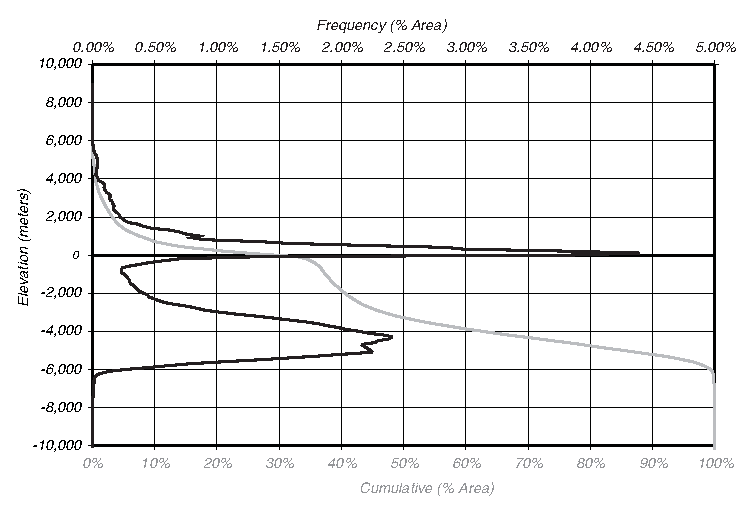
\includegraphics{pics/depth-r}}
\footnotesize
Figure 3.5 Histogram of height\rule{0pt}{3ex} of land and depth of the
sea as percentage of area of earth in 100 m intervals, showing the
clear distinction between continents and sea floor. The cumulative
frequency curve is the integral of the histogram. The curves are
calculated from the \textsc{etopo} 2 data set by George Sharman of the
\textsc{noaa} National Geophysical Data Center.
\label{fig:depth-r}
\vspace{-3ex}
\end{figure}

\begin{figure}[b!]
\centering
\vspace{-2ex}
\makebox[121 mm] [c]{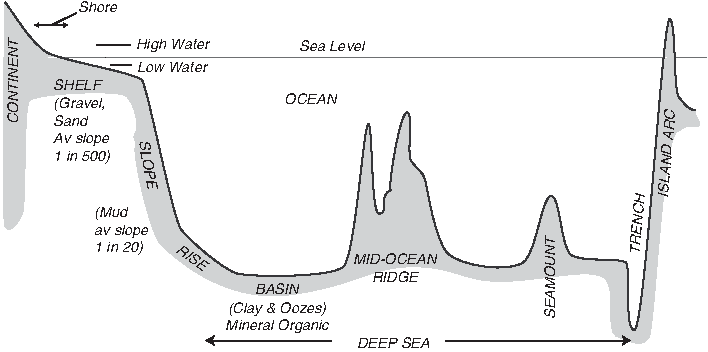
\includegraphics{pics/bathysketch}}
\footnotesize
Figure 3.6 Schematic section through the ocean showing\rule{0pt}{4ex}
principal features of the sea floor. Note that the slope of the sea
floor is greatly exaggerated in the figure.
\label{fig:bathysketch}
%\vspace{-4ex}
\end{figure}

The volume of the water in the ocean exceeds the volume of the ocean
basins, and some water spills over on to the low lying areas of the
continents. These shallow seas are the continental shelves. Some, such
as the South China Sea, are more than 1100 km wide. Most are
relatively shallow, with typical depths of 50--100 m. A few of the
more important shelves are: the East China Sea, the Bering Sea, the
North Sea, the Grand Banks, the Patagonian Shelf, the Arafura Sea and
Gulf of Carpentaria, and the Siberian Shelf. The shallow seas help
dissipate tides, they are often areas of high biological productivity,
and they are usually included in the exclusive economic zone of
adjacent countries.

The crust is broken into large plates that move relative to each
other. New crust is created at the mid-ocean ridges, and old crust is
lost at trenches. The relative motion of crust, due to plate
tectonics, produces the distinctive features of the sea floor sketched
in figure 3.6, including mid-ocean ridges, trenches, island arcs, and
basins.  \index{ocean!features of|(}The names of the sub-sea features
have been defined by the International Hydrographic
Organization\index{International Hydrographic Bureau} (1953), and the
following definitions are taken from Sverdrup, Johnson, and Fleming
(1942), Shepard (1963), and Dietrich et al. (1980).

\textit{Basins} \index{basins|textbf}are deep depressions of the sea
floor of more or less circular or oval form.

\textit{Canyons} \index{canyon|textbf}are relatively narrow, deep
furrows with steep slopes, cutting across the continental shelf and
slope, with bottoms sloping continuously downward.

\textit{Continental shelves} \index{continental shelves|textbf}are
zones adjacent to a continent (or around an island) and extending from
the low-water line to the depth, usually about 120 m, where there is a
marked or rather steep descent toward great depths. (figure 3.7)
\begin{figure}[b!]
\vspace{-2ex}
\makebox[121 mm] [c]{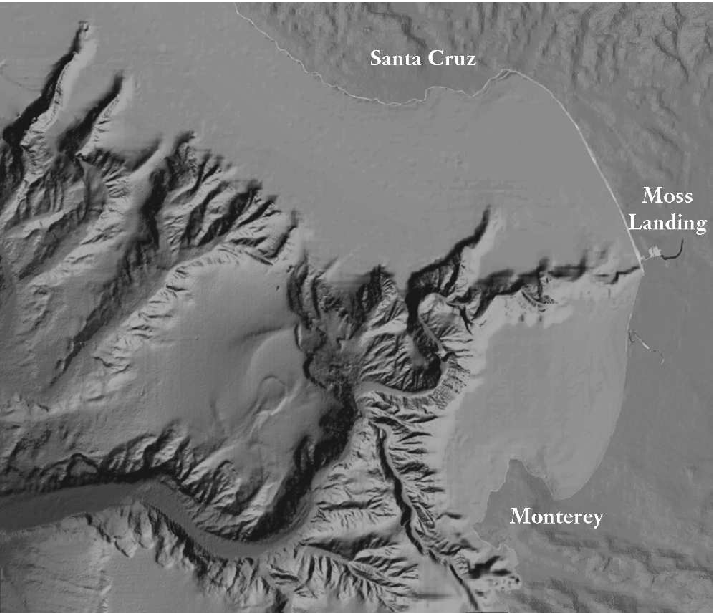
\includegraphics{pics/canyon}}
\footnotesize
Figure 3.7 An example of a continental shelf,\rule{0pt}{3ex} the shelf
offshore of Monterey California showing the Monterey and other
canyons.  Canyons are common on shelves, often extending across the
shelf and down the continental slope to deep water. Figure copyright
Monterey Bay Aquarium Research Institute (\textsc{mbari}).
\label{fig:canyon}
%\vspace{-3ex}
\end{figure}

\textit{Continental slopes} \index{continental slopes|textbf}are the
declivities seaward from the shelf edge into greater depth.

\textit{Plains} \index{plains|textbf}are very flat surfaces found in
many deep ocean basins.

\textit{Ridges} \index{ridges|textbf}are long, narrow elevations of
the sea floor with steep sides and rough topography.

\textit{Seamounts} \index{seamounts|textbf}are isolated or
comparatively isolated elevations rising 1000 m or more from the sea
floor and with small summit area (figure 3.8).

\textit{Sills} \index{sills|textbf}are the low parts of the ridges
separating ocean basins from one another or from the adjacent sea
floor.

\textit{Trenches} \index{trenches|textbf}are long, narrow, and deep
depressions of the sea floor, with relatively steep sides (figure
3.9).\index{ocean!features of|)}

\begin{figure}[t!]
\makebox[121 mm] [c]{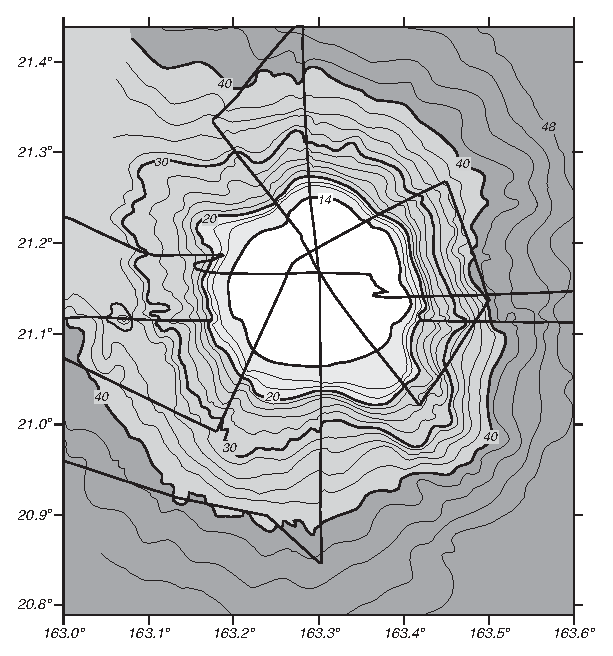
\includegraphics{pics/wildeguyot}}
\footnotesize
Figure 3.8 An example of a seamount, the Wilde Guyot.\rule{0pt}{4ex}
A guyot is a seamount with a flat top created by wave action when the
seamount extended above sea level. As the seamount is carried by plate
motion, it gradually sinks deeper below sea level. The depth was
contoured from echo sounder data collected along the ship track (thin
straight lines) supplemented with side-scan sonar data. Depths are in
units of 100 m. From William Sager, Texas A\&M University.
\label{fig:wildeguyot}
\vspace{-3ex}
\end{figure}

\begin{figure}[t!]
\makebox[121 mm] [c]{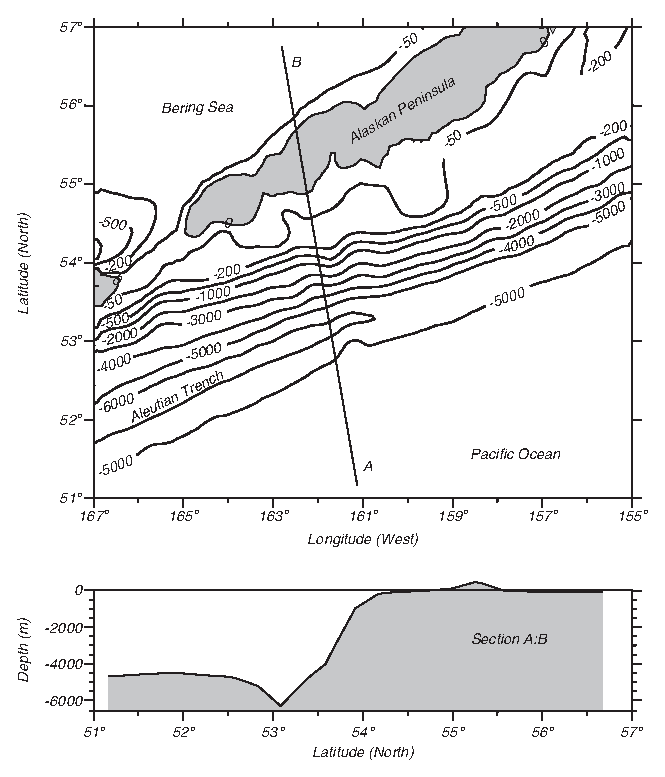
\includegraphics{pics/aleutiantrench}}
\footnotesize
Figure 3.9 An example of a trench, \rule{0pt}{3ex}the Aleutian Trench;
an island arc, the Alaskan Peninsula; and a continental shelf, the
Bering Sea. The island arc is composed of volcanos produced when
oceanic crust carried deep into a trench melts and rises to the
surface. \textbf{Top:} Map of the Aleutian region of the North
Pacific. \textbf{Bottom:} Cross-section through the region.
\label{fig:aleutiantrench}
\vspace{-4ex}
\end{figure}

Sub-sea features strongly influences the ocean circulation.  Ridges
separate deep waters of the ocean into distinct basins. Water deeper
than the sill\index{sills} between two basins cannot move from one to
the other. Tens of thousands of seamounts are scattered throughout the
ocean basins. They interrupt ocean currents, and produce
turbulence\index{turbulence!in deep ocean} leading to vertical
mixing\index{mixing!vertical} in the ocean.

\section{Measuring the Depth of the Ocean}
The depth of the ocean is usually measured two ways: 1) using acoustic
echo-sounders on ships, or 2) using data from satellite altimeters.

\paragraph{Echo Sounders} \index{echo sounders|(}Most maps of the ocean are based
on measurements made by echo sounders. The instrument transmits a
burst of 10--30 kHz sound\index{sound!used to measure depth} and
listens for the echo from the sea floor. The time interval between
transmission of the pulse and reception of the echo, when multiplied
by the velocity of sound, gives twice the depth of the ocean (figure
3.10).

The first transatlantic echo soundings were made by the U.S. Navy
Destroyer \textit{Stewart} in 1922. This was quickly followed by the
first systematic survey of an ocean basin, made by the German research
and survey ship \textit{Meteor} during its expedition to the south
Atlantic from 1925 to 1927. Since then, oceanographic and naval ships
have operated echo sounders almost continuously while at sea. Millions
of miles of ship-track data recorded on paper have been digitized to
produce data bases used to make maps.  The tracks are not well
distributed. Tracks tend to be far apart in the southern hemisphere,
even near Australia (figure 3.11) and closer together in well mapped
areas such as the North Atlantic.\index{echo sounders|)}

\begin{figure}[t!]
\makebox[121 mm] [c] {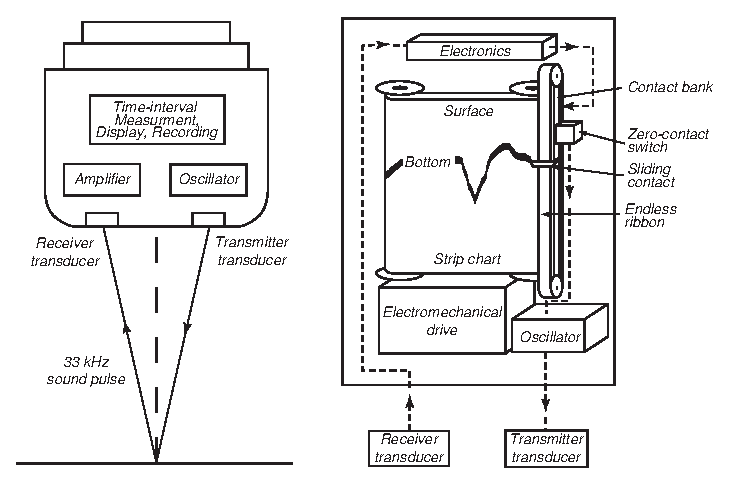
\includegraphics{pics/Sonar}}
%\centering
\footnotesize
Figure 3.10 \textbf{Left:} Echo \rule{0ex}{5ex}sounders measure depth
of the ocean by transmitting pulses of sound\index{sound!used to
  measure depth} and observing the time required to receive the echo
from the bottom. \textbf{Right:} The time is recorded by a spark
burning a mark on a slowly moving roll of paper. After Dietrich et
al. (1980: 124).
\label{fig:Sonar}
\vspace{-3ex}
\end{figure}

\begin{figure}[t!]
%\vspace{-3ex}
\makebox[121 mm] [c]{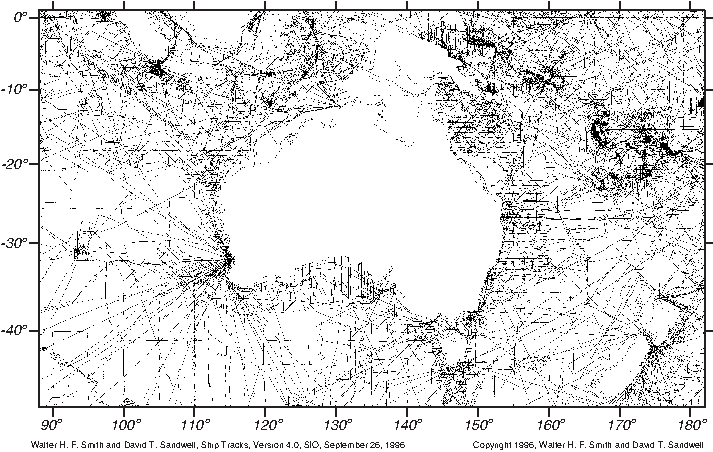
\includegraphics{pics/shiptracks10}}
\footnotesize
%\centering
Figure 3.11 Locations of \rule{0pt}{5ex}echo-sounder data used for
mapping the ocean floor near Australia. Note the large areas where
depths have not been measured from ships. From David Sandwell, Scripps
Institution of Oceanography.

\label{fig:shiptracks10}
\vspace{-3ex}
\end{figure}

Echo sounders \index{echo sounders!errors in measurement}make the most
accurate measurements of ocean depth. Their
accuracy\index{accuracy!echo sounders} is $\pm$1\%.

\paragraph{Satellite Altimetry} \index{satellite altimetry!use in measuring
depth}Gaps in our knowledge of ocean depths between ship tracks have
now been filled by satellite-altimeter data. Altimeters profile the
shape of the sea surface, and its shape is very similar to the shape
of the sea floor (Tapley and Kim, 2001; Cazenave and Royer, 2001;
Sandwell and Smith, 2001). To see this, we must first consider how
gravity influences sea level.

\textit{The Relationship Between Sea Level and the Ocean's Depth}
Excess mass at the sea floor, for example the mass of a seamount,
increases local gravity because the mass of the seamount is larger
than the mass of water it displaces. Rocks are more than three times
denser than water. The excess mass increases local gravity, which
attracts water toward the seamount. This changes the shape of the sea
surface (figure 3.12).

\begin{figure} [t!]
\fbox{\parbox{12cm}{
\centering
\vspace{-0.5 em}
\section*{The Geoid}
\begin{minipage}{11.5cm}
\vspace{0.5 em} \hspace*{1 em}The \index{geoid|textbf}level
surface\index{level surface} that corresponds to the surface of an
ocean at rest is a special surface, the \textit{geoid}. To a first
approximation, the geoid\index{geoid} is an ellipsoid that corresponds
to the surface of a rotating, homogeneous fluid in solid-body
rotation, which means that the fluid has no internal flow. To a second
approximation, the geoid differs from the ellipsoid because of local
variations in gravity. The deviations are called \textit{geoid
  undulations}. \index{geoid!undulations|textbf}The maximum amplitude
of the undulations is roughly $\pm 60$ m. To a third approximation,
the geoid deviates from the sea surface because the ocean is not at
rest. The deviation of sea level from the geoid\index{geoid} is
defined to be the \textit{topography}. \index{topography|textbf}The
definition is identical to the definition for land topography, for
example the heights given on a topographic map.

\hspace*{1 em}The ocean's topography is caused by tides, heat content
of the water, and ocean surface currents. I will return to their
influence in chapters 10 and 17. The maximum amplitude of the
topography is roughly $\pm 1$ m, so it is small compared to the
geoid\index{geoid} undulations.

\hspace*{1 em}Geoid undulations are caused by local variations in
gravity due to the uneven distribution of mass at the sea floor.
Seamounts have an excess of mass because they are more dense than
water. They produce an upward bulge in the geoid (see below). Trenches
have a deficiency of mass. They produce a downward deflection of the
geoid\index{geoid}. Thus the geoid\index{geoid} is closely related to
sea-floor topography. Maps of the oceanic geoid\index{geoid} have a
remarkable resemblance to the sea-floor topography.

\vspace{5ex}
\makebox[118mm][c]{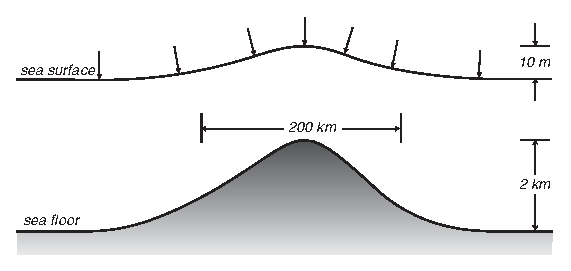
\includegraphics{pics/geoidsketch}}
\footnotesize
Figure 3.12 Seamounts \rule{0mm}{6ex}are more dense than sea
water. They increase local gravity, causing a plumb line at the sea
surface (arrows) to be deflected toward the seamount. Because the
surface of an ocean at rest must be perpendicular to gravity, the sea
surface and the local geoid\index{geoid} must have a slight bulge as
shown. Such bulges are easily measured by satellite altimeters.  As a
result, satellite altimeter data can be used to map the sea
floor. Note, the bulge at the sea surface is greatly exaggerated, a
two-kilometer high seamount would produce a bulge of approximately 10 m.
\label{fig:geoidsketch}
\vspace{0.7ex}
\end{minipage}
}}
\vspace{-4ex}
\end{figure}

Let's make the concept more exact. To a very good approximation, the
sea surface is a particular \textit{level surface} \index{level
  surface|textbf}called the \textit{geoid} (see box). By definition a
level surface is a surface of constant gravitational potential, and it
is everywhere perpendicular to gravity. In particular, it must be
perpendicular to the local vertical determined by a plumb line, which
is ``a line or cord having at one end a metal weight for determining
vertical direction'' (Oxford English Dictionary).

The excess mass of the seamount attracts the plumb line's weight,
causing the plumb line to point a little toward the seamount instead
of toward earth's center of mass. Because the sea surface must be
perpendicular to gravity, it must have a slight bulge above a seamount
as shown in figure 3.12. If there were no bulge, the sea surface would
not be perpendicular to gravity. Typical seamounts produce a bulge
that is 1--20 m high over distances of 100--200 kilometers.  This
bulge is far too small to be seen from a ship, but it is easily
measured by satellite altimeters. Oceanic trenches have a deficit of
mass, and they produce a depression of the sea surface.

The correspondence between the shape of the sea surface and the depth
of the water is not exact. It depends on the strength of the sea
floor, the age of the sea-floor feature, and the thickness of
sediments. If a seamount floats on the sea floor like ice on water,
the gravitational signal is much weaker than it would be if the
seamount rested on the sea floor like ice resting on a table top. As a
result, the relationship between gravity and sea-floor topography
varies from region to region.

Depths measured by acoustic echo sounders are used to determine the
regional relationships. Hence, altimetry is used to interpolate
between acoustic echo sounder measurements (Smith and Sandwell, 1994).

\textit{Satellite-altimeter systems} \index{satellite
  altimetry!systems|textbf}Now let's see how altimeters measure the
shape of the sea surface. Satellite altimeter systems include a radar
to measure the height of the satellite above the sea surface and a
tracking system to determine the height of the satellite in geocentric
coordinates. The system measures the height of the sea surface
relative to the center of mass of earth (figure 3.13). This gives the
shape of the sea surface.

\begin{figure}[t!]
\makebox[121 mm][c]{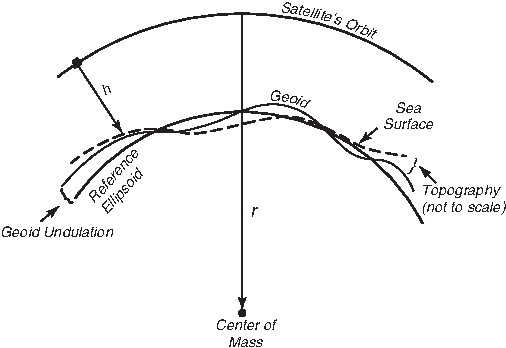
\includegraphics{pics/altimetersketch}}
\footnotesize
Figure 3.13 A satellite altimeter \rule{0mm}{3ex}measures the height
of the satellite above the sea surface. When this is subtracted from
the height $r$ of the satellite's orbit, the difference is sea level
relative to the center of earth. The shape of the surface is due to
variations in gravity, which produce the geoid
undulations\index{geoid!undulations}, and to ocean currents which
produce the oceanic topography, the departure of the sea surface from
the geoid\index{geoid}. The reference ellipsoid is the best smooth
approximation to the geoid. The variations in the geoid, geoid
undulations, and topography are greatly exaggerated in the
figure. From Stewart (1985).
\label{fig:altimetersketch}
\vspace{-4ex}
\end{figure}

Many altimetric satellites have flown in space. All observed the
marine geoid\index{geoid} and the influence of sea-floor features on
the geoid\index{geoid}. The altimeters that produced the most useful
data include Seasat (1978)\index{Seasat}, \textsc{geosat}
(1985--1988), \textsc{ers}--1\index{ERS satellites} (1991--1996),
\textsc{ers}--2 (1995-- ), Topex/Poseidon\index{Topex/Poseidon}
(1992--2006), Jason\index{Jason} (2002--), and Envisat
(2002)\index{Envisat}.  Topex/Poseidon and Jason were specially
designed to make extremely accurate measurements of sea-surface
height. They measure sea-surface height with an accuracy of $\pm 0.05$
m\index{Jason!accuracy of}\index{Topex/Poseidon!accuracy of}.

\textit{Satellite Altimeter Maps of the Sea-floor Topography}
Seasat\index{Seasat}, \textsc{geosat}\index{Geosat}, \textsc{ers}--1,
and \textsc{ers}--2\index{ERS satellites} were \index{satellite
  altimetry!maps of the sea-floor topography}operated in orbits with
ground tracks spaced 3--10 km apart, which was sufficient to map the
geoid\index{geoid}. By combining data from echo-sounders with data
from \textsc{geosat} and \textsc{ers}--1 altimeter systems, Smith and
Sandwell (1997) produced maps of the sea floor with horizontal
resolution of 5--10 km and a global average depth accuracy of $\pm
100$ m.

\section{Sea Floor Charts and Data Sets}
\index{ocean!maps of}Almost all echo-sounder data have been digitized
and combined to make sea-floor charts. Data have been further
processed and edited to produce digital data sets which are widely
distributed in \textsc{cd-rom} format. These data have been
supplemented with data from altimetric satellites to produce maps of
the sea floor with horizontal resolution around 3 km.

The British Oceanographic Data Centre publishes the General
Bathymetric Chart of the ocean (\textsc{gebco})\index{bathymetric
  charts!GEBCO} Digital Atlas on behalf of the Intergovernmental
Oceanographic Commission of \textsc{unesco} and the International
Hydrographic Organization\index{International Hydrographic
  Organization}. The atlas consists primarily of the location of depth
contours, coastlines, and tracklines from the \textsc{gebco} 5th
Edition published at a scale of 1:10 million. The original contours
were drawn by hand based on digitized echo-sounder data plotted on
base maps.

The U.S. National Geophysical Data Center\index{bathymetric
  charts!ETOPO-2} publishes the \textsc{etopo-2 cd-rom} containing
digital values of oceanic depths from echo sounders and altimetry and
land heights from surveys. Data are interpolated to a 2-minute (2
nautical mile) grid. Ocean data between 64\degrees N and 72\degrees S
are from the work of Smith and Sandwell (1997), who combined
echo-sounder data with altimeter data from \textsc{geosat} and
\textsc{ers--1}. Seafloor data northward of 64\degrees N are from the
International Bathymetric Chart of the Arctic Ocean.  Seafloor data
southward of 72\degrees S are from are from the US Naval Oceanographic
Office's Digital Bathymetric Data Base Variable Resolution. Land data
are from the \textsc{globe} Project, that produced a digital elevation
model with 0.5-minute (0.5 nautical mile) grid spacing using data from
many nations.

\begin{figure}[t!]
\makebox[121 mm] [c]{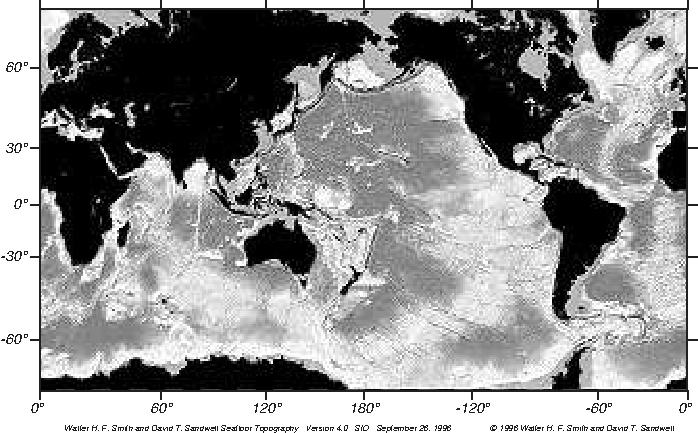
\includegraphics{pics/worldbathym}}
\centering
\footnotesize
Figure 3.14 The sea-floor \rule{0pt}{3ex}topography of the ocean with
3 km resolution produced from satellite altimeter observations of the
shape of the sea surface. From Smith and Sandwell.

\label{fig:worlsbathym}
\vspace{-4ex}
\end{figure}

National governments publish coastal and harbor maps. In the USA, the
\textsc{noaa} National Ocean Service publishes nautical charts useful
for navigation of ships in harbors and offshore waters.

\section{Sound in the Ocean}
Sound\index{sound!in ocean} provides the only convenient means for
transmitting information over great distances in the ocean.
Sound\index{sound!use of} is used to measure the properties of the sea
floor, the depth of the ocean, temperature, and currents. Whales and
other ocean animals use sound to navigate, communicate over great
distances, and find food.

\paragraph{Sound Speed}
The sound speed \index{sound!speed}in the ocean varies with
temperature, salinity, and pressure (MacKenzie, 1981; Munk et
al. 1995: 33):
\begin{align}
  C & = 1448.96 + 4.591\,t - 0.05304\,t^2 + 0.0002374\,t^3+ 0.0160\,Z \\
  &+ (1.340 - 0.01025\,t) (S - 35) + 1.675 \times 10^{-7}\,Z^2 - 7.139 \times
10^{-13}\,t\,Z^3 \notag
\end{align}
where $C$ is speed in m/s, $t$ is temperature in Celsius, $S$ is
salinity (see Chapter 6 for a definition of salinity), and $Z$ is
depth in meters. The equation has an
accuracy\index{accuracy!equation!sound speed} of about 0.1 m/s (Dushaw
et al. 1993). Other sound-speed equations have been widely used,
especially an equation proposed by Wilson (1960) which has been widely
used by the U.S. Navy.

For typical oceanic conditions, $C$ is usually between 1450 m/s and
1550 m/s (figure 3.15). Using (3.1), we can calculate the sensitivity
of $C$ to changes of temperature, depth, and salinity typical of the
ocean. The approximate values are: 40 m/s per 10\degrees C rise of
temperature, 16 m/s per 1000 m increase in depth, and 1.5 m/s per 1
increase in salinity. Thus the primary causes of variability of sound
speed\index{sound!speed!variation of} is temperature and depth
(pressure).  Variations of salinity are too small to have much
influence.

\begin{figure}[t!]
\makebox[121 mm] [c]{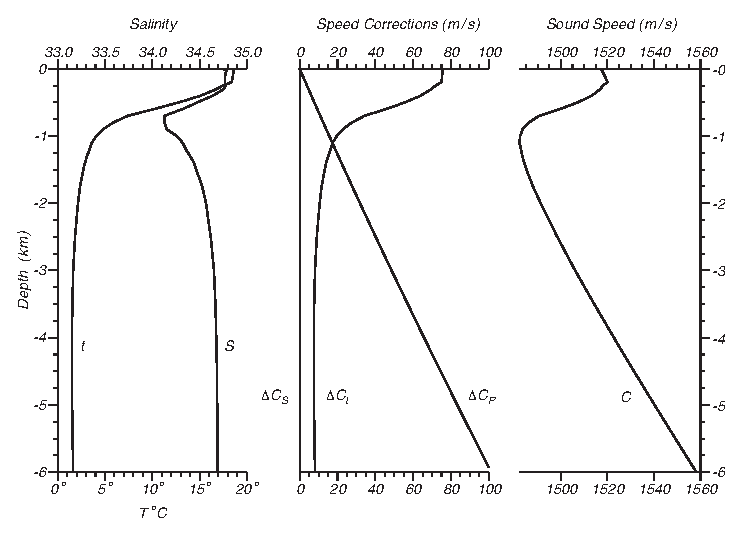
\includegraphics{pics/sound_profile}}
\footnotesize
Figure 3.15 Processes \rule{0pt}{4ex}producing the sound
channel\index{sound!channel} in the ocean.  \textbf{Left:} Temperature
$T$ and salinity $S$ measured as a function of depth during the R.V.
\textit{Hakuho Maru} cruise KH-87-1, station JT, on 28 January 1987 at
Latitude 33\degrees 52.90$'$ N, Long 141\degrees 55.80$'$ E in the
North Pacific.  \textbf{Center:} Variations in sound
speed\index{sound!speed!variation of} due to variations in
temperature, salinity, and depth. \textbf{Right:} Sound
speed\index{sound!speed!as function of depth} as a function of depth
showing the velocity minimum near 1 km depth which defines the sound
channel\index{sound!channel} in the ocean. (Data from \textsc{jpots}
Editorial Panel, 1991).
\label{fig:soundprofile}
\vspace{-3ex}
\end{figure}

If we plot sound speed\index{sound!speed!as function of depth} as a
function of depth, we find that the speed usually has a minimum at a
depth around 1000 m (figure 3.16). The depth of minimum speed is
called the \textit{sound channel}\index{sound!channel|textbf}. It
occurs in all ocean, and it usually reaches the surface at very high
latitudes.

The sound channel\index{sound!channel} is important because sound in
the channel can travel very far, sometimes half way around the
earth. Here is how the channel works: Sound\index{sound!rays} rays
that begin to travel out of the channel are refracted back toward the
center of the channel. Rays propagating upward at small angles to the
horizontal are bent downward, and rays propagating downward at small
angles to the horizontal are bent upward (figure 3.16). Typical depths
of the chan\-nel vary from 10 m to 1200 m depending on geographical
area.

\begin{figure}[t!]
\makebox[121 mm] [c]{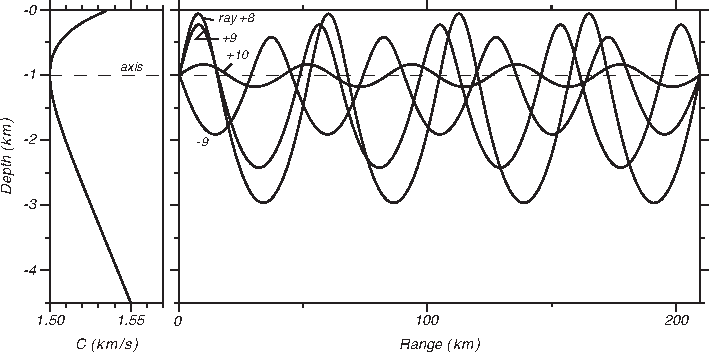
\includegraphics{pics/raypaths}}
\footnotesize
\centering
Figure 3.16 Ray paths of sound\index{sound!rays} in the ocean for a
\rule{0pt}{3ex}source near\\the axis of the sound channel. After Munk
et al. (1995).

\label{fig:raypaths}
\vspace{-3ex}
\end{figure}

\paragraph{Absorption of Sound}
Absorption of sound \index{sound!absorption of}per unit distance
depends on the intensity $I$ of the sound:
\begin{equation}
dI = -k I_0 \, dx
\end{equation}
where $I_0$ is the intensity before absorption and $k$ is an
absorption coefficient which depends on frequency of the sound. The
equation has the solution:
\begin{equation}
I = I_0 \exp(-kx)
\end{equation}
Typical values of $k$ (in decibels dB per kilometer) are: 0.08 dB/km
at 1000 Hz, and 50 dB/km at 100,000 Hz. Decibels are calculated from:
$dB = 10 \log(I/I_0)$, where $I_0$ is the original acoustic power, $I$
is the acoustic power after absorption.

For example, at a range of 1 km a 1000 Hz signal is attenuated by only
1.8\%: $I = 0.982 I_0$. At a range of 1 km a 100,000 Hz signal is
reduced to $I = 10^{-5} I_0$. The 30,000 Hz signal used by typical
echo sounders to map the ocean's depths are little attenuated going
from the surface to the bottom and back.

Very low frequency sounds in the sound channel\index{sound!channel},
those with frequencies below 500 Hz have been detected at distances of
megameters. In 1960 15-Hz sounds from explosions set off in the sound
channel\index{sound!channel} off Perth Australia were heard in the
sound channel near Bermuda, nearly halfway around the world. Later
experiment showed that 57-Hz signals transmitted in the sound channel
near Heard Island (75\degrees E, 53\degrees S) could be heard at
Bermuda in the Atlantic and at Monterey, California in the Pacific
(Munk et al. 1994).

\paragraph{Use of Sound}
Because low frequency sound \index{sound!use of}can be heard at great
distances, the US Navy, in the 1950s, placed arrays of microphones on
the sea floor in deep and shallow water and connected them to shore
stations. The Sound Surveillance System \textsc{sosus}, although
designed to track submarines, has found many other uses. It has been
used to listen to and track whales up to 1,700 km away, and to find
the location of sub-sea volcanic eruptions.

\section{Important Concepts}
\begin{enumerate}
\item If the ocean were scaled down to a width of 8 inches it would
  have depths about the same as the thickness of a piece of paper. As
  a result, the velocity field in the ocean is nearly
  2-dimensional. Vertical velocities are much smaller than horizontal
  velocities.

\vitem There are only three official ocean.

\vitem The volume of ocean water exceeds the capacity of the ocean
basins, and the ocean overflows on to the continents creating
continental shelves.

\vitem The depths of the ocean are mapped by echo sounders which
measure the time required for a sound\index{sound!used to measure
  depth} pulse to travel from the surface to the bottom and
back. Depths measured by ship-based echo sounders have been used to
produce maps of the sea floor. The maps have poor horizontal
resolution in some regions because the regions were seldom visited by
ships and ship tracks are far apart.

\vitem The depths of the ocean are also measured by satellite
altimeter systems which profile the shape of the sea surface. The
local shape of the surface is influenced by changes in gravity due to
sub-sea features. Recent maps based on satellite altimeter
measurements of the shape of the sea surface combined with ship data
have depth accuracy of $ \pm $100 m and horizontal resolutions of $
\pm $3 km.

\vitem Typical sound\index{sound!speed!typical} speed in the ocean is
1480 m/s. Speed depends primarily on temperature, less on pressure,
and very little on salinity. The variability of sound speed as a
function of pressure and temperature produces a horizontal sound
channel in the ocean. Sound in the channel can travel great distances.
Low-frequency sounds below 500 Hz can travel halfway around the world
provided the path is not interrupted by land.
\end{enumerate}


\chapter{Atmospheric Influences} 

The sun \index{sun}and the atmosphere drive directly or indirectly
almost all dynamical processes in the ocean. The dominant external
sources and sinks of energy are sunlight, evaporation, infrared
emissions from the sea surface, and sensible heating of the sea by
warm or cold winds. Winds drive the ocean's surface circulation down
to depths of around a kilometer. Wind and tidal
mixing\index{mixing!tidal} drive the deeper currents in the ocean.

The ocean, in turn, is the dominant source of heat that drives the
atmospheric circulation.\index{atmospheric circulation!driven by
  ocean} The uneven distribution of heat loss and gain by the ocean
leads to winds in the atmosphere.  Sunlight warms the tropical ocean,
which evaporate, transferring heat in the form of water vapor to the
atmosphere. The heat is released when the vapor condenses as
rain. Winds and ocean currents carry heat poleward, where it is lost
to space.

Because the atmosphere drives the ocean, and the ocean drives the
atmosphere, we must consider the ocean and the atmosphere as a coupled
dynamic system. In this chapter we will look mainly at the exchange of
momentum between the atmosphere and the ocean. In the next chapter, we
will look at heat exchanges. In chapter 14 we will look at how the
ocean and the atmosphere interact in the Pacific to produce El
Ni\~{n}o.

\section{The Earth in Space}
Earth's \index{earth!in space}orbit about the sun\index{sun} is nearly
circular at a mean distance of \(1.5 \times 10^8\) km. The
eccentricity of the orbit is small, 0.0168.  Thus earth is 3.4\%
further from the Sun\index{sun} at aphelion than at perihelion, the
time of closest approach to the sun. Perihelion occurs every year in
January, and the exact time changes by about 20 minutes per year. In
1995, it occurred on 3 January. Earth's axis of rotation is inclined
23.45\degrees\ to the plane of earth's orbit around the sun\index{sun}
(figure 4.1). The orientation is such that the sun\index{sun!equinox}
is directly overhead at the Equator on the vernal and autumnal
equinoxes, which occur on or about 21 March and 21 September each
year.

The latitudes of 23.45\degrees\ North and South are the Tropics of
Cancer and Capricorn respectively. The tropics lie equatorward of
these latitudes. As a result of the eccentricity of earth's orbit,
maximum solar insolation\index{insolation!maximum} averaged over the
surface of the earth occurs in early January each year. As a result of
the inclination of earth's axis of rotation, the maximum insolation at
any location outside the tropics occurs around 21 June in the northern
hemisphere, and around 21 December in the southern hemisphere.

\begin{figure}[t!]
\makebox[121 mm] [c] {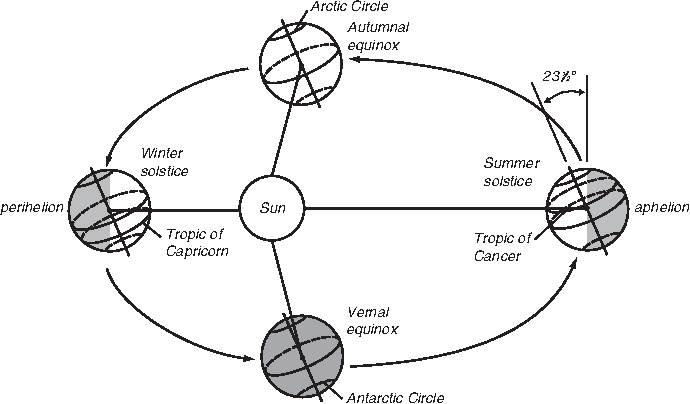
\includegraphics{pics/earthinspace}}
\footnotesize
Figure 4.1 The earth in space. The \rule{0mm}{3ex}ellipticity of
earth's orbit around the sun\index{sun} and the tilt of earth's axis
of rotation relative to the plane of earth orbit leads to an unequal
distribution of heating and to the seasons. Earth is closest to the
sun at perihelion.
\label{fig:earthinspace}
\vspace{-4ex}
\end{figure}

\begin{figure}[b!]
\vspace{-2ex}
\makebox[121 mm] [c] {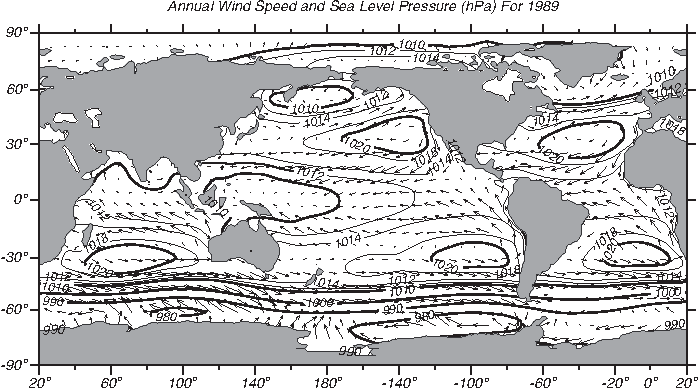
\includegraphics{pics/surfacewind}}
\footnotesize
Figure 4.2 Map of mean annual \index{wind!global map}wind velocity
\rule{0 pt}{3 ex} calculated from Trenberth et al. (1990) and
sea-level pressure for 1989 from the \textsc{nasa} Goddard Space
Flight Center's Data Assimilation Office (Schubert et al. 1993). The
winds near 140\degrees W in the equatorial Pacific are about 8 m/s.
\label{fig:surfacewinds} %\vspace{-3ex}
%\vspace{-3ex}
\end{figure}

If solar heat was rapidly redistributed over earth, maximum
temperature would occur in January. Conversely, if heat were poorly
redistributed, maximum temperature in the northern hemisphere would
occur in summer. So it is clear that heat is not rapidly redistributed
by winds and currents.

\section{Atmospheric Wind Systems}
Figure 4.2 shows the distribution of sea-level winds and pressure
averaged over the year 1989. The map shows strong winds from the west
between 40\degrees\ to 60\degrees\ latitude, the roaring forties, weak
winds in the subtropics near 30\degrees\ latitude, trade winds from
the east in the tropics, and weaker winds from the east along the
Equator. The strength and direction of winds in the atmosphere is the
result of uneven distribution of solar heating and continental land
masses and the circulation of winds in a vertical plane in the
atmosphere.

\begin{figure}[b!]
\vspace{-2ex}
\makebox [121mm][c]{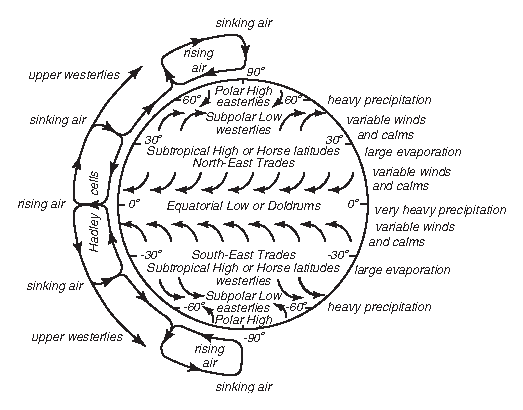
\includegraphics{pics/atmosphereA}}
\makebox [121mm][c]{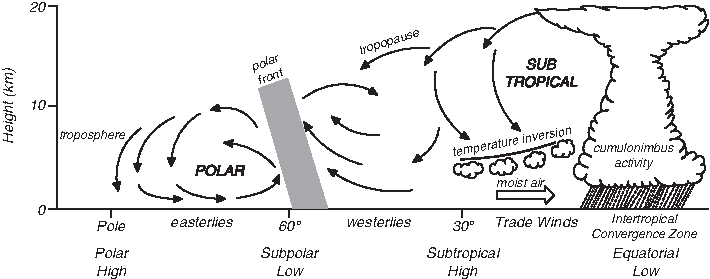
\includegraphics{pics/atmosphereB}}
\footnotesize
Figure 4.3 Sketch of earth's atmospheric \rule{0mm}{3ex}circulation
driven by solar heating in the tropics and cooling at high latitudes.
\textbf{Upper:} The meridional cells in the atmosphere and the
influence of earth's rotation on the winds. \textbf{Bottom:}
Cross-section through the atmosphere showing the two major cells of
meridional circulation. After The Open University (1989a: 14).
\label{fig:atmosphere}
%\vspace{-5ex}
\end{figure}

A cartoon of the distribution of winds in the atmosphere (figure 4.3)
shows that the surface winds are influenced by equatorial convection
and other processes higher in the atmosphere. The mean value
\index{wind!global mean}of winds over the ocean is (Wentz et al. 1984):
\begin{equation}
U_{10} = 7.4 \text{ m/s}
\end{equation}

\begin{figure}[b!]
\vspace{-1ex}
%\centering
\makebox[121 mm] [c] {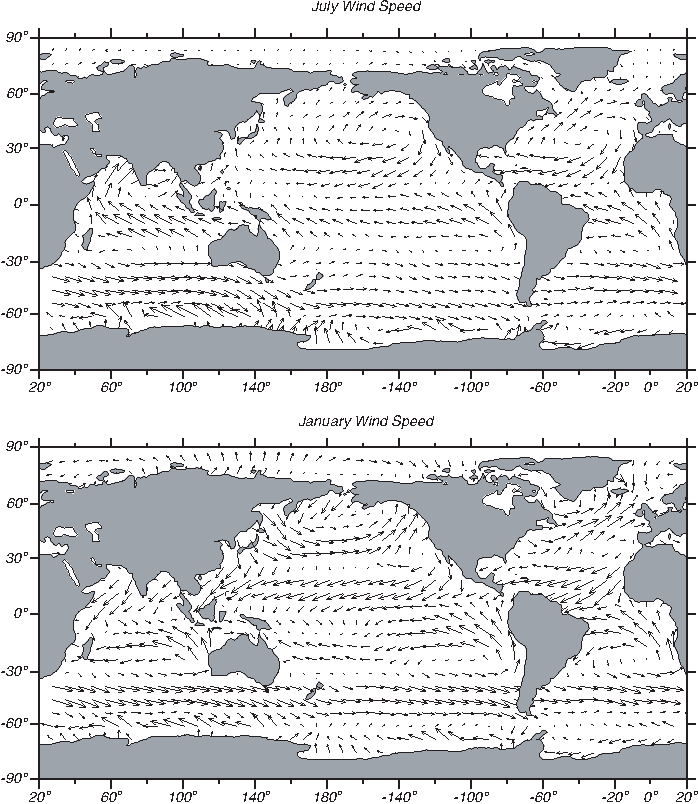
\includegraphics{pics/seasonalwinds}}
\footnotesize
Figure 4.4 Mean, sea-surface \rule{0pt}{3ex}winds for July and January
calculated from the Trenberth et al. (1990) data set, which is based
on the \textsc{ecmwf} reanalyses of weather data from 1980 to
1989. The winds near 140\degrees W in the equatorial Pacific are about 8 m/s.
\label{fig:seasonalwinds}
%\vspace{-3ex}
\end{figure}

Maps of surface winds change somewhat with the seasons. The largest
changes are in the Indian Ocean and the western Pacific Ocean (figure
4.4). Both regions are strongly influenced by the Asian monsoon. In
winter, the cold air mass over Siberia creates a region of high
pressure at the surface, and cold air blows southeastward across Japan
and on across the hot Kuroshio\index{Kuroshio}, extracting heat from
the ocean. In summer, the thermal low over Tibet draws warm, moist air
from the Indian Ocean leading to the rainy season over India.

\section{The Planetary Boundary Layer}
The atmosphere within 100 m of the sea surface is influenced by the
turbulent drag of the wind on the sea and the fluxes of heat through
the surface. This is the \textit{atmospheric boundary
  layer}. \index{atmospheric boundary layer|textbf}It's thickness
$Z_i$ varies from a few tens of meters for weak winds blowing over
water colder than the air to around a kilometer for stronger winds
blowing over water warmer than the air.

The lowest part of the atmospheric boundary layer is the surface
layer. Within this layer, which has thickness of $\approx 0.1 Z_i$,
vertical fluxes of heat and momentum are nearly constant.

Wind speed varies as the logarithm of height within the surface layer
for neutral stability. See ``The Turbulent Boundary Layer Over a Flat
Plate'' in Chapter 8. Hence, the height of a wind measurement is
important. Usually, winds are reported as the value of wind at a
height 10 m above the sea $U_{10}$.

\section{Measurement of Wind}
\index{wind!measurement of|(}Wind at sea has been measured for
centuries. Maury (1855) was the first to systematically collect and
map wind reports. Recently, the US National Atmospheric and Oceanic
Administration \textsc{noaa} has collected, edited, and digitized
millions of observations going back over a century. The resulting
\textit{International Comprehensive Ocean, Atmosphere Data Set}
\textsc{icoads} \index{ICOADS (international comprehensive
  ocean-atmosphere data set)}discussed in \S 5.5 is widely used for
studying atmospheric forcing of the ocean.

Our knowledge of winds at the sea surface come from many sources. Here
are the more important, listed in a crude order of relative
importance:

\paragraph{Beaufort Scale}
\index{wind!Beaufort scale}By far the most common source of wind data
up to 1991 have been reports of speed based on the Beaufort scale. The
scale is based on features, such as foam coverage and wave shape, seen
by an observer on a ship (table 4.1).

The scale was originally proposed by Admiral Sir F. Beaufort in 1806
to give the force of the wind on a ship's sails. It was adopted by the
British Admiralty in 1838 and it soon came into general use.

\begin{table}[t!] {\textbf{\footnotesize{Table 4.1 Beaufort Wind Scale and State of the Sea}}}
\index{wind!Beaufort scale}
\\[1ex]
\begin{footnotesize}
\begin{tabular}{@{}clrp{70mm}@{}} \hline
Beaufort    & Descriptive & m/s & Appearance \rule{0ex}{2.5ex}of the Sea \\
Number & term \  &  & \\[0.5ex]
\hline  %\\
0 & Calm \rule{0ex}{2.5ex}  &   0 & Sea like a mirror. \\
1 & Light Air&  1.2 &   Ripples with appearance of scales; no foam crests.\\
2 & Light Breeze &  2.8 &   Small wavelets; crests of glassy appearance, \\
\ &\ &\ & \hspace{1em}not breaking. \\
3 & Gentle breeze&  4.9 &   Large wavelets; crests begin to break; scattered\\
\ &\ &\ & \hspace{1em}whitecaps.\\
4 & Moderate breeze & 7.7 & Small waves, becoming longer; numerous whitecaps. \\
5 & Fresh breeze &  10.5 &  Moderate waves, taking longer to form; many\\
\ &\ &\ & \hspace{1em}whitecaps; some spray. \\
6 & Strong breeze & 13.1 &  Large waves forming; whitecaps everywhere; \\
\ &\ &\ &\hspace{1em}more spray. \\
7 & Near gale & 15.8 &  Sea heaps up; white foam from breaking waves begins\\
\ &\ &\ & \hspace{1em}to be blown into streaks.\\
8 & Gale &      18.8  & Moderately high waves of greater length; edges of \\
\ &\ &\ & \hspace{1em}crests begin to break into spindrift; foam is blown \\
\ &\ &\ & \hspace{1em}in well-marked streaks.\\
9 & Strong gale &   22.1  & High waves; sea begins to roll; dense streaks of foam;
\\
\ &\ &\ & \hspace{1em}spray may reduce visibility. \\
10 &    Storm &     25.9  & Very high waves with overhanging crests; sea takes \\
\ &\ &\ & \hspace{1em}white appearance as foam is blown in very dense \\
\ &\ &\ & \hspace{1em}streaks; rolling is heavy and visibility reduced. \\
11 &    Violent storm & 30.2  & Exceptionally high waves; sea covered with white \\
\ &\ &\ & \hspace{1em}foam patches; visibility still more reduced.  \\
12 &    Hurricane & 35.2  & Air is filled with foam; sea completely white\\
\ &\ &\ &  \hspace{1em}with driving  \rule[-2.5ex]{0ex}{0.5ex}spray;
visibility greatly reduced.\\
\hline
\end{tabular} \\[0.5ex]
From Kent and Taylor (1997)
\end{footnotesize}
\vspace{-4ex}
\end{table}

The International Meteorological Committee adopted the force scale for
international use in 1874. In 1926 they adopted a revised scale giving
the wind speed at a height of 6 meters corresponding to the Beaufort
Number. The scale was revised again in 1946 to extend the scale to
higher wind speeds and to give the equivalent wind speed at a height
of 10 meters. The 1946 scale was based on the equation $U_{10} = 0.836
B^{3/2}$, where $B = $ Beaufort Number and $U_{10}$ is the wind speed
in meters per second at a height of 10 meters (List, 1966). More
recently, various groups have revised the Beaufort scale by comparing
Beaufort force with ship measurements of winds. Kent and Taylor (1997)
compared the various revisions of the scale with winds measured by
ships having anemometers at known heights. Their recommended values
are given in table 4.1.

Observers on ships everywhere in the world usually report weather
observations, including Beaufort force, at the same four times every
day. The times are at 0000Z, 0600Z, 1200Z and 1800Z, where Z indicates
Greenwich Mean Time. The reports are coded and reported by radio to
national meteorological agencies. The biggest error in the reports is
the sampling error\index{sampling error}. Ships are unevenly
distributed over the ocean. They tend to avoid high latitudes in
winter and hurricanes in summer, and few ships cross the southern
hemisphere (figure 4.5). Overall, the
accuracy\index{accuracy!winds!Beaufort} is around 10\%.


\begin{figure}[t!]
\centering
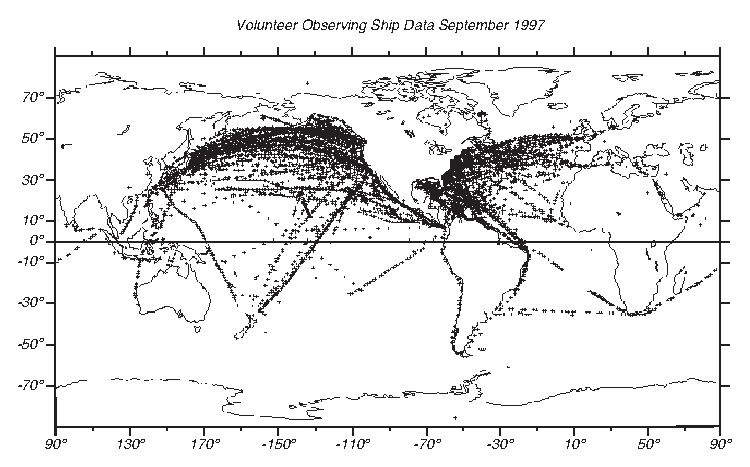
\includegraphics{pics/shiplocations}
\footnotesize
Figure 4.5 Location of surface observations \rule{0mm}{3ex}made from
volunteer observing ships and\\ reported to national meteorological
agencies. From \textsc{noaa}, National Ocean Service.

\label{fig:shiplocations}
\vspace{-4ex}
\end{figure}

\paragraph{Scatterometers}
\index{wind!from scatterometers} \index{scatterometers}Observations of
winds at sea now come mostly from scatterometers on satellites (Liu,
2002). The scatterometer is a instrument very much like a radar that
measures the scatter of centimeter-wavelength radio waves from small,
centimeter-wavelength waves on the sea surface. The area of the sea
covered by small waves, their amplitude, and their orientation, depend
on wind speed and direction. The scatterometer measures scatter from
2--4 directions, from which wind speed and direction are calculated.

The scatterometers on \textsc{ers-1} and 2 have made global
measurements of winds from space since 1991. The \textsc{nasa}
scatterometer\index{scatterometers} on \textsc{adeos} measured winds
for a six-month period beginning November 1996 and ending with the
premature failure of the satellite. It was replaced by another
scatterometer on QuikScat, launched on 19 June
1999. Quikscat\index{scatterometer!Quikscat} views 93\% of the ocean
every 24 hr with a resolution of 25 km.

Freilich and Dunbar (1999) report that, overall, the \textsc{nasa}
scatterometer\index{scatterometers!accuracy of} on \textsc{adeos}
measured wind speed with an
accuracy\index{accuracy!winds!scatterometer} of $\pm 1.3$ m/s. The
error in wind direction was $\pm17$\degrees. Spatial resolution was 25
km.  Data from QuikScat\index{QuikScat} has an accuracy of $\pm 1$ m/s.

Because scatterometers\index{scatterometers} view a specific oceanic
area only once a day, the data must be used with numerical weather
models to obtain 6-hourly wind maps required for some studies.

\paragraph{Windsat}
Windsat\index{Windsat} is an experimental, polarimetric, microwave
radiometer developed by the US Navy that measures the amount and
polarization of microwave radiation emitted from the sea at angles
between 50\degrees\ to 55\degrees\ relative to the vertical and at
five radio frequencies. It was launched on 6 January 2003 on the
Coriolis satellite. The received radio signal is a function of wind
speed, sea-surface temperature, water vapor in the atmosphere, rain
rate, and the amount of water in cloud drops. By observing several
frequencies simultaneously, data from the instrument are used for
calculating the surface wind speed and direction, sea-surface
temperature, total precipitable water, integrated cloud liquid water,
and rain rate over the ocean regardless of time of day or cloudiness.

Winds are calculated over most of the ocean on a 25-km grid once a
day. Winds measured by Windsat have an accuracy of $\pm 2$ m/s in
speed and $\pm 20$\degrees\ in direction over the range of 5--25 m/s.

\paragraph{Special Sensor Microwave SSM/I}
Another satellite instrument that is used to measure wind speed is the
Special-Sensor Microwave/Imager (\textsc{ssm/i}) carried since 1987 on
the satellites of the U.S. Defense Meteorological Satellite Program in
orbits similar to the \textsc{noaa} polar-orbiting meteorological
satellites. The instrument measures the microwave radiation emitted
from the sea at an angle near 60\degrees\ from the vertical. The radio
signal is a function of wind speed, water vapor in the atmosphere, and
the amount of water in cloud drops. By observing several frequencies
simultaneously, data from the instrument are used for calculating the
surface wind speed, water vapor, cloud water, and rain rate.

Winds measured by \textsc{ssm/i} have an
accuracy\index{accuracy!winds!SSM/I} of $\pm$ 2 m/s in speed. When
combined with \textsc{ecmwf} 1000 mb wind analyses, wind direction can
be calculated with an accuracy of $\pm 22$\degrees\ (Atlas, Hoffman,
and Bloom, 1993). Global, gridded data are available since July 1987
on a 0.25\degrees\ grid every 6 hours. But remember, the instrument
views a specific oceanic area only once a day, and the gridded,
6-hourly maps have big gaps.

\paragraph{Anemometers on Ships}
Satellite observations are supplemented by winds reported to
meteorological agencies by observers reading ane\-mom\-eters on
ships. The anemometer is read four times a day at the standard
Greenwich times and reported via radio to meteorological agencies.

Again, the biggest error is the sampling error\index{sampling
  error}. Very few ships carry calibrated anemometers. Those that do
tend to be commercial ships participating in the Volunteer Observing
Ship program (figure 4.5). These ships are met in port by scientists
who check the instruments and replace them if necessary, and who
collect the data measured at sea.  The
accuracy\index{accuracy!winds!ship} of wind measurements from these
ships is about $\pm 2$ m/s.

\paragraph{Calibrated Anemometers on Weather Buoys}
The most accurate measurements of winds at sea are made by calibrated
anemometers on moored weather buoys. Unfortunately there are few such
buoys, perhaps only a hundred scattered around the world. Some, such
as Tropical Atmosphere Ocean \textsc{tao} array in the tropical
Pacific (figure 14.14) provide data from remote areas rarely visited
by ships, but most tend to be located just offshore of coastal areas.
\textsc{noaa} operates buoys offshore of the United States and the
\textsc{tao} array in the Pacific. Data from the coastal buoys are
averaged for eight minutes before the hour, and the observations are
transmitted to shore via satellite links.

The best accuracy of anemometers on buoys operated by the \textsc{us}
National Data Buoy Center is the greater of \(\pm\)1 m/s or 10\% for
wind speed and $\pm 10$\degrees\ for wind direction (Beardsley et
al. 1997).\index{wind!measurement of|)}

\section{Calculations of Wind}
\index{numerical models!numerical weather models}Satellites, ships,
and buoys measure winds at various locations and times of the day. If
you wish to use the observations to calculate monthly averaged winds
over the sea, then the observations can be averaged and gridded. If
you wish to use wind data in numerical models of the ocean's currents,
then the data will be less useful. You are faced with a very common
problem: How to take all observations made in a six-hour period and
determine the winds over the ocean on a fixed grid?

One source of gridded winds over the ocean is the \textit{surface
  analysis}\index{surface analysis|textbf} calculated by numerical
weather models\index{wind!from numerical weather models}. The strategy
used to produce the six-hourly gridded winds is called
\textit{sequential estimation techniques} \index{sequential estimation
  techniques|textbf}or \textit{data assimilation}\index{data
  assimilation|textbf}. ``Measurements are used to prepare initial
conditions for the model, which is then integrated forward in time
until further measurements are available. The model is thereupon
re-initialized'' (Bennett, 1992: 67). The initial condition is called
the \textit{analysis}.

Usually, all available measurements are used in the analysis,
including observations from weather stations on land, pressure and
temperature reported by ships and buoys, winds from
scatterometers\index{scatterometers}\index{wind!from scatterometers}
in space, and data from meteorological satellites. The model
interpolates the measurements to produce an analysis consistent with
previous and present observations. Daley (1991) describes the
techniques in considerable detail.

\paragraph{Surface Analysis from Numerical Weather Models}
Perhaps the most widely used weather model is that run by the European
Centre for Medium-range Weather Forecasts \textsc{ecmwf}. It
calculates a surface analysis\index{surface analysis}, including
surface winds and heat fluxes\index{heat flux} (see Chapter 5) every
six hours on a 1\degrees\ $ \times $ 1\degrees\ grid from an explicit
boundary-layer model. Calculated values are archived on a 2.5\degrees
grid. Thus the wind maps from the numerical weather models lack the
detail seen in maps from scatterometer data, which have a
1/4\degrees\ grid.

\textsc{ecmwf} calculations of winds have relatively good
accuracy\index{accuracy!winds!calculated}. Freilich and Dunbar (1999)
estimated that the accuracy for wind speed at 10 meters is $\pm 1.5$
m/s, and $\pm 18$\degrees\ for direction.

Accuracy in the southern hemisphere is probably as good as in the
northern hemisphere because continents do not disrupt the flow as much
as in the northern hemisphere, and because
scatterometers\index{scatterometers} give accurate positions of storms
and fronts over the ocean.

The \textsc{noaa} National Centers for Environmental Prediction and
the US Navy also produces global analyses and forecasts every six
hours.

\paragraph{Reanalyzed Data from Numerical Weather Models}
\index{numerical models!numerical weather models!reanalysis
  from}\index{wind!from numerical weather models}Surface analyses of
weather over some regions have been produced for more than a hundred
years, and over the whole earth since about 1950. Surface analyses
calculated by numerical models of the atmospheric circulation have
been available for decades. Throughout this period, the methods for
calculating surface analyses have constantly changed as meteorologists
worked to make ever more accurate forecasts. Fluxes calculated from
the analyses are therefore not consistent in time. The changes can be
larger than the interannual variability of the fluxes (White,
1996). To minimize this problem, meteorological agencies have taken
all archived weather data and reanalyzed them using the best numerical
models to produce a uniform, internally-consistent, surface
analysis\index{surface analysis}.

The reanalyzed data are used to study oceanic and atmospheric
processes in the past. Surface analyses\index{surface analysis} issued
every six hours from weather agencies are used only for problems that
require up-to-date information. For example, if you are designing an
offshore structure, you will probably use decades of reanalyzed
data. If you are operating an offshore structure, you will watch the
surface analysis and forecasts put out every six hours by
meteorological agencies.

\paragraph{Sources of Reanalyzed Data}
\index{numerical models!numerical weather models!sources of reanalyzed
  data}Reanalyzed surface flux data are available from national
meteorological centers operating numerical weather prediction models.

\begin{enumerate}
\vitem The U.S. National Centers for Environmental Predictions,
working with the National Center for Atmospheric Research have
produced the \textsc{ncep/ ncar} reanalysis based on 51 years of
weather data from 1948 to 2005 using the 25 January 1995 version of
their forecast model. The reanalysis period is being extended forward
to include all date up to the present with about a three-day delay in
producing data sets. The reanalysis uses surface and ship observations
plus sounder data from satellites.  Reanalysis products are available
every six hours on a T62 grid having $192 \times 94$ grid points with
a spatial resolution of 209 km and with 28 vertical levels. Important
subsets of the reanalysis, including surface fluxes, are available on
\textsc{cd--rom} (Kalnay et al. 1996; Kistler et al. 2000).

\vitem The European Centre for Medium-range Weather Forecasts
\textsc{ecmwf} has reanalyzed 45 years of weather data from September
1957 to August 2002 (\textsc{era}-40) using their forecast model of
2001 (Uppala et al. 2005). The reanalysis uses mostly the same surface
and ship data used by the \textsc{ncep/ncar} reanalysis plus data from
the \textsc{ers}-1 and \textsc{ers}-2\index{ERS satellites} satellites
and \textsc{ssm/i}. The \textsc{era}-40 full-resolution products are
available every six hours on a N80 grid having $160 \times 320$ grid
points with a spatial resolution of 1.125\degrees\ and with 60
vertical levels. The \textsc{era}-40 basic-resolution products are
available every six hours with a spatial resolution of
2.5\degrees\ and with 23 vertical levels. The reanalysis includes an
ocean-wave model that calculates ocean wave heights and wave spectra
every six hours on a 1.5\degrees\ grid.
\end{enumerate}

\section{Wind Stress}
\index{wind stress|textbf}The wind, by itself, is usually not very
interesting. Often we are much more interested in the force of the
wind, or the work done by the wind. The horizontal force of the wind
on the sea surface is called the \textit{wind stress}. Put another
way, it is the vertical transfer of horizontal momentum. Thus momentum
is transferred from the atmosphere to the ocean by wind stress.

Wind stress $T$ is calculated from:

\begin{equation}
T = \rho_a \,C_D U_{10}^2
\end{equation}
where $\rho_a = 1.3$ kg/m$^3$ is the density of air, $U_{10}$ is wind
speed at 10 meters, and $C_D$ is the \textit{drag
  coefficient}\index{drag!coefficient|textbf}.  $C_D$ is measured
using the techniques described in \S5.6. Fast response instruments
measure wind fluctuations within 10--20 m of the sea surface, from
which $T$ is directly calculated. The correlation of $T$ with
$U_{10}^2$ gives $C_D$ (figure 4.6).

Various measurements of $C_D$ have been published based on careful
measurements of turbulence\index{turbulence!measurement of} in the
marine boundary layer. Trenberth et al.  (1989) and Harrison (1989)
discuss the accuracy\index{accuracy!drag coefficient} of an effective
drag coefficient\index{drag!coefficient} relating wind
stress\index{wind stress!and drag coefficient} to wind velocity on a
global scale. Perhaps the best of the recently published values are
those of Yelland and Taylor (1996) and Yelland et al.  (1998) who
give:

\begin{figure}[t!]
%\vspace{-1ex}
\makebox[121mm] [c] {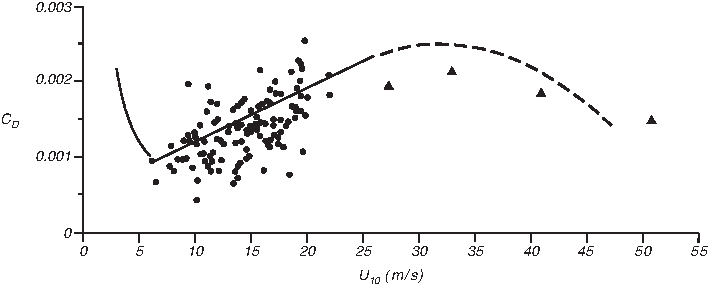
\includegraphics{pics/dragcoefficient}}
\footnotesize
Figure 4.6 The drag\rule{0mm}{3ex} coefficient as a function of wind
speed $U_{10}$ ten meters above the sea. Circles: Measured values from
Smith (1980). Triangles: Measured values from Powell, Vickery, and
Reinhold (2003). The solid line is from eq (4.3) proposed by Yelland
and Taylor (1996). The dashed line is from Jarosz (2007).
\label{fig:dragcoefficient}
\vspace{-3ex}
\end{figure}

\begin{subequations}
\begin {align}
1000 \, C_D = & \,0.29 + \frac{3.1}{U_{10}} + \frac{7.7}{U_{10}^2} & \left( 3 \le
U_{10}
\le 6 \text{ m/s}\right) \\
 1000 \, C_D = & \,0.60 + 0.071 \, U_{10} & \left( 6 \le U_{10} \le 26 \text{ m/s}
\right)
\end{align}
\end{subequations}
for neutrally stable boundary layer. Other values are listed in their
table 1 and in figure 4.6.

\section{Important Concepts}

\begin{enumerate}
\item
Sunlight is the primary energy source driving the atmosphere and
ocean.
\vitem
There is a boundary layer at the bottom of the atmosphere where wind
speed decreases with as the boundary is approached, and in which
fluxes of heat and momentum are constant in the lower 10--20 meters.
\vitem
Wind is measured many different ways. The most common until 1995 was
from observations made at sea of the Beaufort
force\index{wind!Beaufort scale} of the wind.
\vitem
Since 1995, the most important source of wind measurements is from
scatterometers\index{scatterometers}\index{wind!from scatterometers}
on satellites. They produce daily global maps with 25 km resolution.
\vitem
The surface analysis from numerical models of the
atmosphere\index{wind!from numerical weather models} is the most
useful source of global, gridded maps of wind velocity for dates
before 1995. It also is a useful source for 6-hourly maps. Resolution
is 100-250 km.
\vitem
The flux of momentum from the atmosphere to the ocean, the wind
stress\index{wind stress}, is calculated from wind speed using a drag
coefficient\index{drag!coefficient}.
\end{enumerate}


\chapter{The Oceanic Heat Budget}
About half the solar energy reaching earth is absorbed by the ocean
and land, where it is temporarily stored near the surface. Only about
a fifth of the available solar energy is directly absorbed by the
atmosphere. Of the energy absorbed by the ocean, most is released
locally to the atmosphere, mostly by evaporation and infrared
radiation. The remainder is transported \index{transport!heat}by
currents to other areas especially mid latitudes.

Heat lost by the tropical ocean is the major source of heat needed to
drive the atmospheric circulation.  And, solar energy stored in the
ocean from summer to winter helps ameliorate earth's climate. The
thermal energy transported by ocean currents is not steady, and
significant changes in the transport, particularly in the Atlantic,
may have been important for the development of the ice ages. For these
reasons, oceanic heat budgets and transports are important for
understanding earth's climate and its short and long term variability.

\section{The Oceanic Heat Budget}
\index{heat budget|textbf}Changes in energy stored in the upper ocean
result from an imbalance between input and output of heat through the
sea surface. This transfer of heat across or through a surface is
called a \textit{heat flux}\index{heat flux|textbf}. The flux of heat
and water also changes the density of surface waters, and hence their
buoyancy. As a result, the sum of the heat and water fluxes is often
called the \textit{buoyancy flux}\index{buoyancy
  flux|textbf}\index{flux!buoyancy}.

The flux of energy to deeper layers is usually much smaller than the
flux through the surface. And, the total flux of energy into and out
of the ocean must be zero, otherwise the ocean as a whole would heat
up or cool down. The sum of the heat fluxes into or out of a volume of
water is the \textit{heat budget}.\index{heat budget!terms of}

The major terms in the budget at the sea surface are:
\begin{enumerate}
\vitem \textit{Insolation} $Q_{SW}$, \index{insolation|textbf}the flux
of solar energy into the sea;

\vitem \textit{Net Infrared Radiation} $Q_{LW}$, \index{net infrared
  radiation|textbf}net flux of infrared radiation from the sea;

\vitem \textit{Sensible Heat Flux} $Q_S$, \index{sensible heat
  flux|textbf}the flux of heat out of the sea due to conduction;

\vitem \textit{Latent Heat Flux} $Q_L$, \index{latent heat
  flux|textbf}the flux of energy carried by evaporated water; and

\vitem \textit{Advection} $Q_V$, \index{advection|textbf}heat carried
away by currents.
\end{enumerate}

Conservation of heat requires:
\begin{equation}Q = Q_{SW} + Q_{LW} + Q_S + Q_L + Q_V \end{equation}
where $Q$ is the resultant heat gain or loss. Units for heat
fluxes\index{heat flux!units of} are watts/m$^2$. The product of flux
times surface area times time is energy in joules. The change in
temperature $\Delta t$ of the water is related to change in energy
$\Delta E$ through:
\begin{equation}
\Delta E = C_{p} \, m \, \Delta t
\end{equation}
where $m$ is the mass of water being warmed or cooled, and $C_p$ is
the specific heat of sea water at constant pressure.
\begin{equation}
C_{p} \approx 4.0\times 10^{3} \mbox{ J}\cdot \mbox{kg}^{-1} \cdot \, ^\circ
\mbox{C}^{-1}
\end{equation}
Thus, 4,000 joules of energy are required to heat 1.0 kilogram of sea
water by 1.0$^{\circ}$C (figure 5.1).

\begin{figure}[t!]
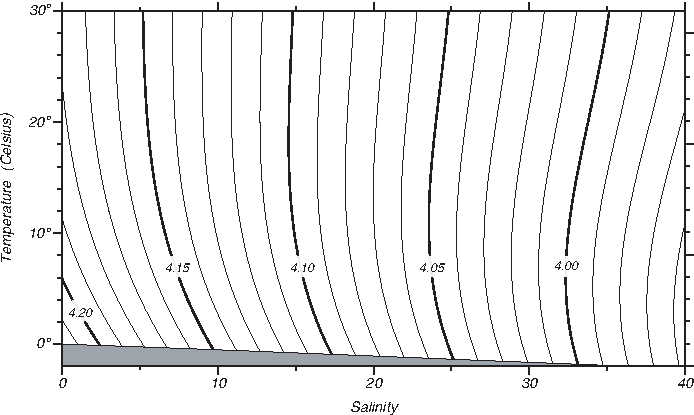
\includegraphics{pics/Cp}
\footnotesize
Figure 5.1 Specific heat of \rule{0pt}{3ex}sea water at atmospheric
pressure $C_{p}$ in joules per gram per degree Celsius as a function
of temperature in Celsius and salinity, calculated from the empirical
formula given by Millero et al. (1973) using algorithms in Fofonoff
and Millard (1983). The lower line is the freezing point of salt
water.
\label{fig:Cp}
\vspace{-3ex}
\end{figure}

\paragraph{Importance of the Ocean in Earth's Heat Budget}
\index{heat budget!importance of}To understand the importance of the
ocean in earth's heat budget, let's make a comparison of the heat
stored in the ocean with heat stored on land during an annual
cycle. During the cycle, heat is stored in summer and released in the
winter. The point is to show that the ocean store and release much
more heat than the land.

To begin, use (5.3) and the heat capacity of soil and rocks
\begin{equation}
C_{p(rock)} = 800 \mbox{ J}\cdot \mbox{kg}^{-1} \cdot \, ^\circ \mbox{C}^{-1}
\end{equation}
to obtain $C_{p(rock)} \approx 0.2 \, C_{p(water)}$.

The volume of water which exchanges heat with the atmosphere on a
seasonal cycle is 100 m$^3$ per square meter of surface, i.e. that
mass from the surface to a depth of 100 meters. The density of water
is 1000 kg/m$^3$, and the mass in contact with the atmosphere is
density $\times$ volume = $m_{water} = 100,000$ kg. The volume of land
which exchanges heat with the atmosphere on a seasonal cycle is 1
m$^3$. Because the density of rock is 3,000 kg/m$^3$, the mass of the
soil and rock in contact with the atmosphere is 3,000 kg.

The seasonal heat storage\index{heat storage!seasonal} values for the
ocean and land are therefore:
\begin{align}
\Delta E_{ocean} & = C_{p(water)} \, m_{water}\, \Delta t && \Delta t =
10^{\circ} \text{C} \notag \\
                                     & = (4000) (10^5) (10^{\circ}) \text{
Joules}       \notag  \\
                                     & = 4.0 \times 10^9 \, \text{Joules}                 \notag  \\
\Delta E_{land}   & = C_{p(rock)} \, m_{rock}\, \Delta t & & \Delta t = 20^{\circ
} \text{C} \notag \\
                                     & = (800) (3000) (20^{\circ}) \text{
Joules}        \notag  \\
                                     & = 4.8 \times 10^7 \, \text{Joules}               \notag  \\
\frac{\Delta E_{ocean}}{\Delta E_{land}}  & = 100 \notag
\end{align}
where $\Delta t$ is the typical change in temperature from summer to
winter.

The large storage of heat in the ocean compared with the land has
important consequences. The seasonal range of air temperatures on land
increases with distance from the ocean, and it can exceed 40\degrees C
in the center of continents, reaching 60\degrees C in Siberia. Typical
range of temperature over the ocean and along coasts is less than
10\degrees C. The variability of water temperatures is still smaller
(see figure 6.3, bottom).

\section{Heat-Budget Terms}
\index{heat budget!terms of}Let's look at the factors influencing each
term in the heat budget.

\paragraph{Factors Influencing Insolation}
\index{insolation!factors influencing}Incoming solar radiation is
primarily determined by latitude, season, time of day, and
cloudiness. The polar regions are heated less than the tropics, areas
in winter are heated less than the same area in summer, areas in early
morning are heated less than the same area at noon, and cloudy days
have less sun than sunny days.

The following factors are important:
\begin{enumerate}
\vitem
The height of the sun\index{sun!height above horizon} above the
horizon, which depends on latitude, season, and time of day. Don't
forget, there is no insolation\index{insolation} at night!
\vitem
The length of day, which depends on latitude and season.
\vitem
The cross-sectional area of the surface absorbing sunlight, which
depends on height of the sun above the horizon.
\vitem
Attenuation, which depends on: i) Clouds, which absorb and scatter
radiation. ii) Path length through the atmosphere, which varies as
$\csc \varphi$, where $\varphi$ is angle of the sun above the
horizon. iii) Gas molecules which absorb radiation in some bands
(figure 5.2). H$_2$O, O$_3$, and CO$_2$ are all important. iv)
Aerosols which scatter and absorb radiation. Both volcanic and marine
aerosols are important. And v) dust, which scatters radiation,
especially Saharan dust over the Atlantic.
\vitem
Reflectivity of the surface, which depends on solar elevation angle
and roughness of sea surface.
\end{enumerate}
Solar inclination and cloudiness dominate. Absorption by ozone, water
vapor, aerosols, and dust are much weaker.

\begin{figure}[t!]
\makebox [121 mm] [c] {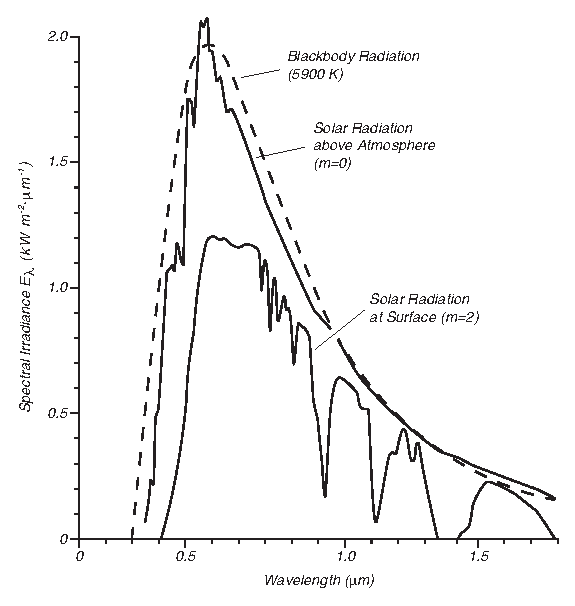
\includegraphics{pics/insolation}}
\footnotesize
Figure 5.2 Insolation\index{insolation!at top of atmosphere}
\rule{0pt}{3ex}(spectral irradiance) of sunlight at top of the
atmosphere and at the sea surface on a clear day. The dashed line is
the best-fitting curve of blackbody radiation the size and distance of
the sun.  The number of standard atmospheric masses is designated by
$m$. Thus $m = 2$ is applicable for sunlight when the
sun\index{sun!height above horizon} is 30\degrees above the
horizon. After Stewart (1985: 43).
\label{fig:insolation}
\vspace{-3ex}
\end{figure}

\begin{figure}[t!]
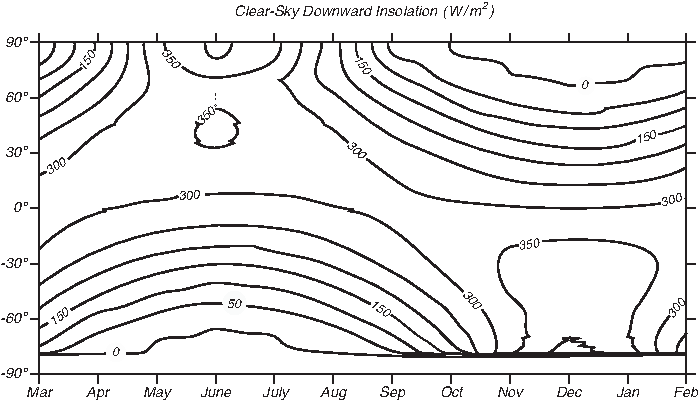
\includegraphics{pics/QswDown}
\footnotesize
Figure 5.3 Monthly average of \rule{0pt}{3ex}downward flux of sunlight
through a cloud-free sky and into the ocean in W/m$^2$ during 1989
calculated by the Satellite Data Analysis Center at the \textsc{nasa}
Langley Research Center (Darnell et al. 1992) using data from the
International Satellite Cloud Climatology Project.
\label{fig:QswDown}
\vspace{-3ex}
\end{figure}

The average annual value for insolation\index{insolation!annual
  average} (figure 5.3) is in the range:
\begin{equation}
30 \text{\ W/m$^2$} < Q_{SW} < 260 \text{\ W/m$^2$}
\end{equation}

\paragraph{Factors Influencing Infrared Flux}
\index{infrared flux!factors influencing}The sea surface radiates as a
blackbody having the same temperature as the water, which is roughly
290 K. The distribution of radiation as a function of wavelength is
given by Planck's equation. Sea water at 290 K radiates most strongly
at wavelengths near 10 $\mu$m. These wavelengths are strongly absorbed
by clouds, and somewhat by water vapor. A plot of atmospheric
transmittance as a function of wavelength for a clear atmosphere but
with varying amounts of water vapor (figure 5.4) shows the atmosphere
is nearly transparent in some wavelength bands called windows.

\begin{figure}[t!]
\makebox [121 mm] [c] {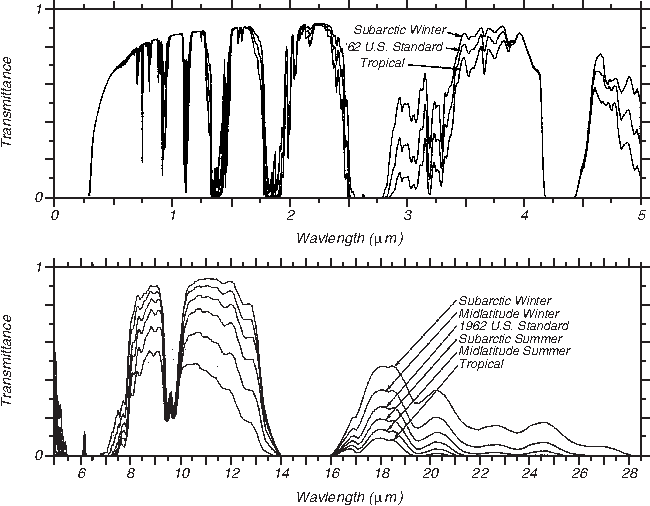
\includegraphics{pics/transmittance}}
\footnotesize
Figure 5.4 Atmospheric \rule{0pt}{3ex}transmittance\index{atmospheric
  transmittance} for a vertical path to space from sea level for six
model atmospheres with very clear, 23 \textit{km}, visibility,
including the influence of molecular and aerosol scattering. Notice
how water vapor modulates the transparency of the 10-14 $\mu$m
atmospheric window, hence it modulates $Q_{LW}$, which is a maximum at
these wavelengths.  After Selby and McClatchey (1975).
\label{fig:transmittance}
\vspace{-3ex}
\end{figure}

The transmittance on a cloud-free day through the window from 8 $\mu$m
to 13 $\mu$m is determined mostly by water vapor. Absorption in other
bands, such as those at 3.5 $\mu$m to 4.0 $\mu$m depends on CO$_2$
concentration in the atmosphere. As the concentration of CO$_2$
increases, these windows close and more radiation is trapped by the
atmosphere.

Because the atmosphere is mostly transparent to incoming sunlight, and
somewhat opaque to outgoing infrared radiation, the atmosphere traps
radiation. The trapped radiation, coupled with convection in the
atmosphere, keeps earth's surface 33\degrees\ warmer than it would be
in the absence of a convecting, wet atmosphere but in thermal
equilibrium with space. The atmosphere acts like the panes of glass on
a greenhouse, and the effect is known as the \textit{greenhouse
  effect}\index{greenhouse effect|textbf}. See Hartmann (1994: 24--26)
for a simple discussion of the radiative balance of a planet. CO$_2$,
water vapor, methane, and ozone are all important greenhouse gasses.

The net infrared flux\index{infrared flux!net} depends on:
\begin{enumerate}
\vitem Clouds thickness. The thicker the cloud deck, the less heat
escapes to space.

\vitem Cloud height, which determines the temperature at which the
cloud radiates heat back to the ocean. The rate is proportional to
$t^4$, where $t$ is the temperature of the radiating body in
Kelvins. High clouds are colder than low clouds.

\vitem Atmospheric water-vapor content. The more humid the atmosphere
the less heat escapes to space.

\vitem Water Temperature. The hotter the water the more heat is
radiated.  Again, radiation depends of $t^4$.

\vitem Ice and snow cover. Ice emits as a black body, but it cools
much faster than open water. Ice-covered seas are insulated from the
atmosphere.
\end{enumerate}

Water vapor and clouds influence the net loss of infrared radiation
more than surface temperature. Hot tropical regions lose less heat
than cold polar regions. The temperature range from poles to equator
is $0^{\circ}\rm{C} < t < 25^{\circ}\rm{C}$ or $273\rm{K} < t <
298\rm{K}$, and the ratio of maximum to minimum temperature in Kelvins
is 298/273 = 1.092. Raised to the fourth power this is 1.42. Thus
there is a 42\% increase in emitted radiation from pole to
equator. Over the same distance water vapor can change the net emitted
radiance by 200\%.

The average annual value for net infrared flux\index{infrared
  flux!annual average} is in the narrow range:
\begin{equation}
-60 \text{\ W/m$^2$} < Q_{LW} < -30 \text{\ W/m$^2$}
\end{equation}

\paragraph{Factors Influencing Latent-Heat Flux}
\index{latent heat flux}Latent heat flux is influenced primarily by
wind speed and relative humidity. High winds and dry air evaporate
much more water than weak winds with relative humidity near 100\%. In
polar regions, evaporation from ice covered ocean is much less than
from open water. In the arctic, most of the heat lost from the sea is
through leads (ice-free areas). Hence the percent open water is very
important for the arctic heat budget.

The average annual value for latent-heat flux is in the range:
\begin{equation}
-130 \text{\ W/m$^2$} < Q_{L} < -10 \text{\ W/m$^2$}
\end{equation}

\paragraph{Factors Influencing Sensible-Heat Flux}
\index{sensible heat flux}Sensible heat flux is influenced by wind
speed and air-sea temperature difference. High winds and large
temperature differences cause high fluxes. Think of this as a
wind-chill factor for the ocean.

The average annual value for sensible-heat flux is in the range:
\begin{equation}
-42 \text{\ W/m$^2$} < Q_{S} < -2 \text{\ W/m$^2$}
\end{equation}

\section[Direct Calculation of Fluxes]{Direct Calculation of Fluxes}
Before we can describe the geographical distribution of fluxes into
and out of the ocean, we need to know how they are measured or
calculated.

\paragraph{Gust-Probe Measurements of Turbulent Fluxes}
\index{flux!direct calculation of!gust probe measurement}There is only
one accurate method for calculating fluxes of sensible and latent heat
and momentum at the sea surface: from direct measurement of turbulent
quantities in the atmospheric boundary layer made by gust probes on
low-flying aircraft or offshore platforms. Very few such measurements
have been made. They are expensive, and they cannot be used to
calculate heat fluxes\index{heat flux!measurements of} averaged over
many days or large areas. The gust-probe measurements are used only to
calibrate other methods of calculating fluxes.

\begin{enumerate}
\vitem Measurements must be made in the surface layer of the
atmospheric boundary layer (See \S 4.3), usually within 30 m of the
sea surface, because fluxes are independent of height in this layer.
\vitem Measurements must be made by fast-response instruments (gust
probes) able to make several observations per second on a tower, or
every meter from a plane.
\vitem Measurements include the horizontal and vertical components of
the wind, the humidity, and the air temperature.
\end{enumerate}

Fluxes are calculated from the correlation of vertical wind and
horizontal wind, humidity, or temperature: Each type of flux is
calculated from different measured variables, $u'$, $w'$, $t'$, and
$q'$:
\begin{subequations}
\begin{align}
T &= \langle \rho_a \,{u'w'}\rangle = \rho_a \, \langle {u'w'}\rangle \equiv \rho_a \,u_*^2\\
Q_S &= C_p\,\langle\rho_a\,{w't'}\rangle = \rho_a \, {C_p} \, \langle{w't'}\rangle \\ 
Q_L &= L_E \, \langle{w'q'}\rangle
\end{align}
\end{subequations}
where the brackets denotes time or space averages, and the notation is
given in table 5.1. Note that \textit{specific
  humidity}\index{specific humidity|textbf} mentioned in the table is
the mass of water vapor per unit mass of air.

\begin{table}[t!]\small
\begin{tabular*}{121mm}{@{}llc@{}}
\multicolumn{3}{@{}l@{}}{\bfseries Table 5.1 Notation \rule[-1ex]{0mm}{1ex}Describing Fluxes}         \\
\hline
Symbol   &  Variable    \rule{0mm}{2.5ex}                  & Value and Units                          \\
\hline
$C_p$    &  Specific heat capacity of air\rule{0mm}{2.5ex} & 1030 J$\cdot$kg$^{-1}\cdot$K$^{-1}$      \\
$C_D$    &  Drag coefficient  (see 4.3)                    & $(0.50 + 0.071 \, U_{10})\times
10^{-3}$ \\
$C_L$    &  Latent heat transfer coefficient               & $1.2 \times 10^{-3}$                     \\
$C_S$    &  Sensible heat transfer coefficient             & $1.0 \times 10^{-3}$                     \\
$L_E$    &  Latent heat of evaporation                     & $2.5 \times 10^6$ J/kg                   \\
$q$      &  Specific humidity of air                       & kg (water vapor)/kg (air)                \\
$q_a$    &  Specific humidity of air 10 m above the sea    & kg (water vapor)/kg (air)                \\
$q_s$    &  Specific humidity of air at the sea surface    & kg (water vapor)/kg (air)                \\
$Q_S$    &  Sensible heat flux                             & W/m$^{2}$                                \\
$Q_L$    &  Latent heat flux                               & W/m$^{2}$                                \\
$T$      &  Wind stress                                    & Pascals                                  \\
$t_a$    &  Temperature of the air 10 m above the sea      & K or
$^{\circ}$C                         \\
$t_s$    &  Sea-surface temperature                        & K or
$^{\circ}$C                         \\
$t'$     &  Temperature fluctuation                        & $^{\circ}C$                              \\
$u'$     &  Horizontal component of fluctuation of wind    & m/s                                      \\
$u_*$    &  Friction velocity                              & m/s                                      \\
$U_{10}$ &  Wind speed at 10 m above the sea               & m/s                                      \\
$w'$     &  Vertical component of wind fluctuation         & m/s                                      \\
$\rho_a$   &  Density of air                                 & 1.3 kg/m$^{3}$                           \\
$T$      &  Vector wind stress                             &
Pa                                       \\ [0.5ex]
\hline
\end{tabular*} \\ [0.5ex]
$C_S$ and $C_L$ from Smith (1988).
\vspace {-3ex}
\end{table}

\paragraph{Radiometer Measurements of Radiative Fluxes}
\index{flux!direct calculation of!radiometer measurements}Radiometers
on ships, offshore platforms, and even small islands are used to make
direct measurements of radiative fluxes. Wideband radiometers
sensitive to radiation from 0.3 $\mu$m to 50 $\mu$m can measure
incoming solar and infrared radiation with an
accuracy\index{accuracy!fluxes!radiative} of around 3\% provided they
are well calibrated and maintained. Other, specialized radiometers can
measure the incoming solar radiation, the downward infrared radiation,
and the upward infrared radiation.

\section{Indirect Calculation of Fluxes: Bulk Formulas}
\index{flux!indirect calculation of!bulk formulas}The use of
gust-probes is very expensive, and radiometers must be carefully
maintained. Neither can be used to obtain long-term, global values of
fluxes. To calculate these fluxes from practical measurements, we use
observed correlations between fluxes and variables that can be
measured globally.

For fluxes of sensible and latent heat and momentum, the correlations
are called \textit{bulk formulas}. \index{bulk formulas|textbf}They
are:
\begin{subequations}
\begin{align}
T     & = \rho_a \,C_D \, U^{2}_{10} \\
Q_S   & = \rho_a \, C_p \,C_S \, U_{10} \, (t_s - t_a) \\
Q_L   & = \rho_a \,  L_E  \, C_L \, U_{10} \,(q_s - q_a)
\end{align}
\end{subequations}

Air temperature $t_a$ is measured using thermometers on ships. It
cannot be measured from space using satellite instruments. $t_s$ is
measured using thermometers on ships or from space using infrared
radiometers such as the \textsc{avhrr}\index{Advanced Very High
  Resolution Radiometer (AVHRR)}.

The specific humidity of air at 10 m above the sea surface $q_a$ is
calculated from measurements of relative humidity made from
ships. Gill (1982: pp: 39--41, 43--44, \& 605--607) describes
equations relating water vapor pressure, vapor density, and specific
heat capacity of wet air. The specific humidity at the sea surface
$q_s$ is calculated from $t_s$ assuming the air at the surface is
saturated with water vapor. $U_{10}$ is measured or calculated using
the instruments or techniques described in Chapter 4. Note that wind
stress\index{wind stress!is a vector} is a vector with magnitude and
direction. It is parallel to the surface in the direction of the wind.

The problem now becomes: How to calculate the fluxes across the sea
surface required for studies of ocean dynamics? The fluxes include: 1)
stress; 2) solar heating; 3) evaporation; 4) net infrared radiation;
5) rain; 5) sensible heat; and 6) others such as CO$_2$ and particles
(which produce marine aerosols). Furthermore, the fluxes must be
accurate. We need an accuracy\index{accuracy!heat fluxes} of
approximately $\pm$15 W/m$^2$. This is equivalent to the flux of heat
which would warm or cool a column of water 100 m deep by roughly
1\degrees{C} in one year. Table 5.2 lists typical accuracies of fluxes
measured globally from space. Now, let's look at each variable.

\begin{table}[t!]\small \centering
\begin{tabular*}{120mm}{@{}lll@{}}
\multicolumn{3}{@{}l@{}}{\bfseries Table 5.2 Accuracy of \rule[-1ex]{0mm}{1ex}Wind
and Fluxes Observed Globally From Space} \\
\hline
Variable         & Accuracy          & Comments   \rule{0mm}{2.5ex}             \\
\hline
Wind Speed       & $\pm$1.5 m/s      & Instrument Error\rule{0ex}{2.5ex}        \\
                 & $\pm$1.5 m/s      & Sampling Error (Monthly Average)         \\
Wind Stress       & $\pm$10 \%        & Drag Coefficient Error\rule{0ex}{2.5ex}  \\
                 & $\pm$14 Pa        & Assuming 10 m/s Wind Speed               \\
Insolation       & $\pm$5 \%         & Monthly Average\rule{0ex}{2.5ex}         \\
                 & $\pm$15 W/m$^2$   & Monthly Average                          \\
                 & $\pm$10 \%        & Daily Average                            \\
Rain Rate        & $\pm$50 \%        &  \rule{0ex}{2.5ex}                       \\
Rainfall         & $\pm$10 \%        & $5^{\circ} \times 5^{\circ}$ area for \textsc{trmm}\rule{0ex}{2.5ex} \\
Net Long Wave Radiation & $\pm$4--8 \%  & Daily Average\rule{0ex}{2.5ex}        \\
                        & $\pm$15--27 W/m$^2$  &                                \\
Latent Heat Flux & $\pm$35 W/m$^2$   & Daily Average\rule{0ex}{2.5ex}           \\
                                                                    & $\pm$15 W/m$^2$   & Monthly Average                          \\ [0.5ex]
\hline
\end{tabular*} \\[0.5ex]
\vspace{-3ex}
\end{table}

\paragraph{Wind Speed and Stress}
\index{wind stress!calculation of}\index{wind!speed}Stress is
calculated from wind observations made from ships at sea and from
scatterometers\index{scatterometers}\index{wind!from scatterometers}
in space as described in the last chapter.

\paragraph{Insolation}
\index{insolation!calculation of} is calculated from cloud
observations made from ships and from visible-light radiometers on
meteorological satellites. Satellite measurements are far more
accurate than the ship data because it's very hard to measure
cloudiness from below the clouds. Satellite measurements processed by
the International Satellite Cloud Climatology Project \textsc{isccp}
are the basis for maps of insolation\index{insolation!maps of} and its
variability from month to month (Darnell et al. 1988; Rossow and
Schiffer 1991).

The basic idea behind the calculation of
insolation\index{insolation!calculation of} is this. Sunlight at the
top of the atmosphere is accurately known from the solar
constant\index{solar constant!and insolation}, latitude, longitude,
and time. Sunlight is either reflected back to space by clouds, or it
eventually reaches the sea surface. Only a small and nearly constant
fraction is absorbed in the atmosphere. But, recent work by Cess et
al. (1995) and Ramanathan et al. (1995) suggest that this basic idea
may be incomplete, and that atmospheric absorption may be a function
of cloudiness. Assuming atmospheric absorption is constant,
insolation\index{insolation!calculation of} is calculated from:
\[
\text{Insolation} = S (1 - A) - C
\]
where $S = 1365$ W/m$^2$ is the solar constant\index{solar
  constant!value}, $A$ is albedo, the ratio of incident to reflected
sunlight, and $C$ is a constant which includes absorption by ozone and
other atmospheric gases and by cloud droplets. Insolation is
calculated from cloud data (which also includes reflection from
aerosols) collected from instruments such as the \textsc{avhrr}
\index{Advanced Very High Resolution Radiometer (AVHRR)}on
meteorological satellites.  Ozone and gas absorption are calculated
from known distributions of the gases in the atmosphere. Q$_{SW}$ is
calculated from satellite data with an
accuracy\index{accuracy!short-wave radiation} of 5--7\%.

\paragraph{Water Flux In (Rainfall)}
\index{flux!water flux!calculation of}\index{water flux!calculation
  of}\index{rainfall!calculation of}Rain rate is another variable that
is very difficult to measure from ships. Rain collected from gauges at
different locations on ships and from gauges on nearby docks all
differ by more than a factor of two. Rain at sea falls mostly
horizontally because of wind, and the ship's superstructure distorts
the paths of raindrops. Rain in many areas falls mostly as drizzle,
and it is difficult to detect and measure.

The most accurate measurements of rain rate in the tropics
($\pm 35$\degrees) are calculated from microwave radiometers and radar
observations of rain at several frequencies using instruments on the
Tropical Rain Measuring Mission \textsc{trmm} launched in 1997. Rain
for other times and latitudes can be calculated accurately by
combining microwave data with infrared observations of the height of
cloud tops and with rain gauge data (figure 5.5). Rain is also
calculated from the reanalyses weather data by numerical models of the
atmospheric circulation (Schubert, Rood, and Pfaendtner, 1993), and by
combining ship and satellite observations with analyses from numerical
weather-prediction models (Xie and Arkin, 1997).

The largest source of error is due to conversion of rain rate to
cumulative rainfall\index{rainfall!cumulative}, a sampling
error\index{sampling error}. Rain is very rare, it is log-normally
distributed, and most rain comes from a few storms. Satellites tend to
miss storms, and data must be averaged over areas up to 5\degrees\ on
a side to obtain useful values of rainfall.

\begin{figure}[t!]
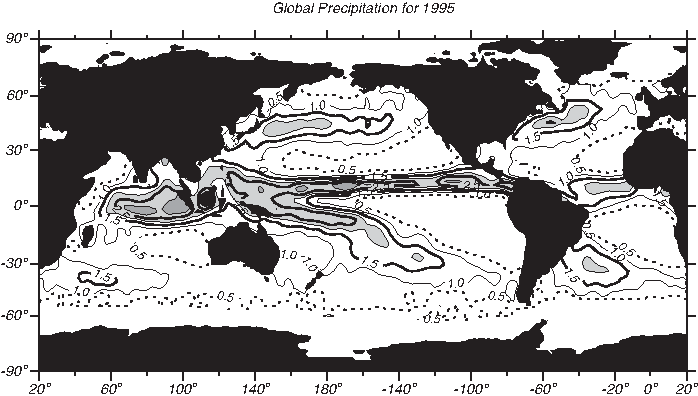
\includegraphics{pics/precip} 
\footnotesize Figure 5.5 Rainfall\index{rainfall!map}
\rule{0pt}{3ex}in m/year calculated \index{global precipitation!map
  of}from data compiled by the Global Precipitation Climatology
Project at \textsc{nasa}'s Goddard Space Flight Center using data from
rain gauges, infrared radiometers on geosynchronous meteorological
satellites, and the \textsc{ssm/i}.  Contour interval is 0.5 m/yr,
light shaded areas exceed 2 m/yr, heavy shaded areas exceed 3
m/yr. \label{fig:precip}
\vspace{-4ex}
\end{figure}

\paragraph{Net Long-Wave Radiation}
\index{flux!net long-wave radiation}\index{net long-wave radiation}Net
Long-wave radiation is not easily calculated because it depends on the
height and thickness of clouds, and the vertical distribution of water
vapor in the atmosphere. It is calculated by numerical
weather-prediction models or from observations of the vertical
structure of the atmosphere from atmospheric sounders.

\paragraph{Water Flux Out (Latent Heat Flux)}
\index{flux!latent heat flux!calculation of}\index{latent heat
  flux!calculation of} Latent heat flux is calculated from ship
observations of relative humidity, water temperature, and wind speed
using bulk formulas (5.10c) and ship data accumulated in the
\textsc{icoads} \index{ICOADS (international comprehensive
  ocean-atmosphere data set)}described below. The fluxes are not
calculated from satellite data because satellite instruments are not
very sensitive to water vapor close to the sea. Perhaps the best
fluxes are those calculated from numerical weather models.

\paragraph{Sensible Heat Flux}
\index{flux!sensible heat flux!calculation of}\index{sensible heat
  flux!calculation of}Sensible heat flux is calculated from
observations of air-sea temperature difference and wind speed made
from ships, or by numerical weather models. Sensible fluxes are small
almost everywhere except offshore of the east coasts of continents in
winter when cold, Arctic air masses extract heat from warm, western,
boundary currents. In these areas, numerical models give perhaps the
best values of the fluxes. Historical ship report give the long-term
mean values of the fluxes.

\section{Global Data Sets for Fluxes}
\index{flux!global data sets for}Ship and satellite data have been
processed to produce global maps of fluxes. Ship measurements made
over the past 150 years yield maps of the long-term mean values of the
fluxes, especially in the northern hemisphere. Ship data, however, are
sparse in time and space, and they are being replaced more and more by
fluxes calculated by numerical weather models and by satellite data.

The most useful maps are those made by combining level 3 and 4
satellite data sets with observations from ships, using numerical
weather models. Let's look first at the sources of data, then at a few
of the more widely used data sets.

\paragraph{International Comprehensive Ocean-Atmosphere Data Set}
\index{ICOADS (international comprehensive ocean-atmosphere data
  set)|textbf}Data collected by observers on ships are the richest
source of marine information. Slutz et al.  (1985) describing their
efforts to collect, edit, and publish all marine observations write:
\begin{quotation} \small
Since 1854, ships of many countries have been taking regular observations
of local weather, sea surface temperature, and many other characteristics
near the boundary between the ocean and the atmosphere. The observations
by one such ship-of-opportunity at one time and place, usually incidental
to its voyage, make up a marine report. In later years fixed research
vessels, buoys, and other devices have contributed data. Marine reports
have been collected, often in machine-readable form, by various agencies and
countries. That vast collection of data, spanning the ocean from
the mid-nineteenth century to date, is the historical ocean-atmosphere record.
\end{quotation}
These marine reports have been edited and published as the
\textit{International Comprehensive Ocean-Atmos\-phere Data Set}
\textsc{icoads} \index{ICOADS (international comprehensive
  ocean-atmosphere data set)}(Woodruff et al.  1987) available through
the National Oceanic and Atmospheric Administration.

The \textsc{icoads} release 2.3 includes 213 million reports of marine
surface conditions collected from 1784--2005 by buoys, other platform
types, and by observers on merchant ships. The data set include fully
quality-controlled (trimmed) reports and summaries. Each unique report
contains 22 observed and derived variables, as well as flags
indicating which observations were statistically trimmed or subjected
to adaptive quality control. Here, statistically trimmed means
outliers were removed from the data set. The summaries included in the
data set give 14 statistics, such as the median and mean, for each of
eight observed variables: air and sea surface temperatures, wind
velocity, sea-level pressure, humidity, and cloudiness, plus 11
derived variables.

The data set consists of an easily-used data base at three principal
resolutions: 1) individual reports, 2) year-month summaries of the
individual reports in 2\degrees \ latitude by 2\degrees \ longitude
boxes from 1800 to 2005 and 1\degrees \ latitude by 1\degrees
\ longitude boxes from 1960 to 2005, and 3) decade-month
summaries. Note that data from 1784 through the early 1800s are
extremely sparse--based on scattered ship voyages.

Duplicate reports judged inferior by a first quality control process
designed by the National Climatic Data Center \textsc{ncdc} were
eliminated or flagged, and ``untrimmed'' monthly and decadal summaries
were computed for acceptable data within each 2\degrees\ latitude by
2\degrees\ longitude grid. Tighter, median-smoothed limits were used
as criteria for statistical rejection of apparent outliers from the
data used for separate sets of \textit{trimmed} monthly and decadal
summaries. Individual observations were retained in report form but
flagged during this second quality control process if they fell
outside 2.8 or 3.5 estimated standard- deviations about the smoothed
median applicable to their 2\degrees\ latitude by 2\degrees\ longitude
box, month, and 56--, 40--, or 30--year period (\textit{i.e.},
1854--1990, 1910--1949, or 1950--1979).

The data are most useful in the northern hemisphere, especially the
North Atlantic.  Data are sparse in the southern hemisphere and they
are not reliable south of 30\degrees\ S. Gleckler and Weare (1997)
analyzed the accuracy\index{accuracy!fluxes!ICOADS} of the
\textsc{icoads} data for calculating global maps and zonal averages of
the fluxes from 55\degrees N to 40\degrees S. They found that
systematic errors dominated the zonal means. Zonal averages of
insolation\index{insolation!zonal average} were uncertain by about
10\%, ranging from $\pm 10$ W/m$^2$ in high latitudes to $\pm 25$
W/m$^2$ in the tropics. Long wave fluxes were uncertain by about $\pm
7$ W/m$^2$. Latent heat flux uncertainties ranged from $\pm 10$
W/m$^2$ in some areas of the northern ocean to $\pm 30$ W/m$^2$ in the
western tropical ocean to $\pm 50$ W/m$^2$ in western boundary
currents. Sensible heat flux\index{sensible heat flux!uncertainty}
uncertainties tend to be around $\pm 5- 10$ W/m$^2$.

Josey et al (1999) compared averaged fluxes calculated from
\textsc{icoads} with fluxes calculated from observations made by
carefully calibrated instruments on some ships and buoys. They found
that mean flux into the ocean, when averaged over all the seas surface
had errors of $\pm 30$ W/m$^2$. Errors vary seasonally and by region,
and global maps of fluxes require corrections such as those proposed
by DaSilva, Young, and Levitus (1995) shown in figure 5.7.

\paragraph{Satellite Data}
Raw data are available from satellite projects, but we need processed
data. Various levels of processed data from satellite projects are
produced (table 5.3):

\begin{table}[h!]\small \centering \vspace{-1ex}
\begin{tabular*}{120mm}{@{}ll@{}}
\multicolumn{2}{@{}l@{}}{\bfseries Table 5.3 Levels of
\rule[-1ex]{0mm}{1ex}Processed Satellite Data}
\\
\hline
Level     & Level of Processing\rule{0mm}{2.5ex}                                              \\
\hline
Level 1   & Data from the satellite in engineering units (volts)\rule{0ex}{2.5ex} \\
Level 2   & Data processed into geophysical units (wind speed) at the time and place          \\
          &   the satellite instrument made the observation                                   \\
Level 3   & Level 2 data interpolated to fixed coordinates in time and space                  \\
Level 4   & Level 3 data averaged in time and space or further processed                      \\[0.5ex]
\hline
\end{tabular*} \\[0.5ex]
\vspace{-2ex}
\end{table}

The operational meteorological satellites that observe the ocean
include:
\begin{enumerate}
\vitem \textsc{noaa} series of polar-orbiting, meteorological satellites;
\vitem U.S. Defense Meteorological Satellite Program \textsc{dmsp} polar-orbiting
satellites, which carry the Special Sensor Microwave/ Imager \textsc{(ssm/i)};
\vitem Geostationary meteorological satellites operated by \textsc{noaa}
(\textsc{goes}), Japan (\textsc{gms}) and the European Space Agency
(\textsc{meteosats}).
\end{enumerate}
Data are also available from instruments on experimental satellites such
as:
\begin{enumerate}
\vitem Nimbus-7, Earth Radiation Budget Instruments;
\vitem Earth Radiation Budget Satellite, Earth Radiation Budget Experiment;
\vitem The European Space Agency's \textsc{ers}--1 \& 2\index{ERS satellites};
\vitem The Japanese ADvanced Earth Observing System (\textsc{adeos}) and Midori;
\vitem QuikScat\index{QuikScat};
\vitem The Earth-Observing System satellites Terra, Aqua, and Envisat;
\vitem The Tropical Rainfall Measuring Mission (\textsc{trmm}); and,
\vitem Topex/Poseidon\index{Topex/Poseidon} and its replacement Jason-1\index{Jason}.
\end{enumerate}

Satellite data are collected, processed, and archived by government
organizations. Archived data are further processed to produce useful
flux data sets.

\paragraph{International Satellite Cloud Climatology Project}
\index{International Satellite Cloud Climatology Project}The
International Sat\-ellite Cloud Climatology Project is an ambitious
project to collect observations of clouds made by dozens of
meteorological satellites from 1983 to 2000, to calibrate the the
satellite data, to calculate cloud cover using carefully verified
techniques, and to calculate surface
insolation\index{insolation!calculation of} and net surface infrared
fluxes (Rossow and Schiffer, 1991). The clouds were observed with
visible-light instruments on polar-orbiting and geostationary
satellites.

\paragraph{Global Precipitation Climatology Project} This project uses three sources
of \index{Global Precipitation Climatology Project}data to calculate
rain rate (Huffman, et al. 1995, 1997):
\begin{enumerate}
\vitem
Infrared observations of the height of cumulus clouds from
\textsc{goes} satellites. The basic idea is that the more rain
produced by cumulus clouds, the higher the cloud top, and the colder
the top appears in the infrared. Thus rain rate at the base of the
clouds is related to infrared temperature.

\vitem
Measurements by rain gauges on islands and land.

\vitem
Radio emissions from water drops in the atmosphere observed by
\textsc{ssm--i}.
\end{enumerate}
Accuracy\index{accuracy!rainfall} is about 1 mm/day. Data from the
project are available on a 2.5\degrees\ latitude by
2.5\degrees\ longitude grid from July 1987 to December 1995 from the
Global Land Ocean Precipitation Analysis at the \textsc{nasa} Goddard
Space Flight Center.

Xie and Arkin (1997) produced a 17-year data set based on seven types
of satellite and rain-gauge data combined with the rain calculated
from the \textsc{ncep/ncar} reanalyzed data from numerical weather
models. The data set has the same spatial and temporal resolution as
the Huffman data set.

\paragraph{Reanalyzed Output From Numerical Weather Models}
\index{numerical models!numerical weather models!reanalyzed data
  from}Surface heat flux\index{heat flux!from numerical models} has
been calculated from weather data using numerical weather models by
various reanalysis projects described in \S 4.5. The fluxes are
consistent with atmospheric dynamics, they are global, they are
calculated every six hours, and they are available for many years on a
uniform grid. For example, the \textsc{ncar/ncep} reanalysis,
available on a \textsc{cd-rom}, include daily averages of wind
stress\index{wind stress!daily averages of}, sensible and latent heat
fluxes, net long and short wave fluxes, near-surface temperature, and
precipitation.

\paragraph{Accuracy of Calculated Fluxes}
Recent studies of the accuracy\index{accuracy!fluxes!from models} of
fluxes computed by numerical weather models and reanalysis projects
suggest:
\begin{enumerate}
\vitem
Heat fluxes from the \textsc{ncep} and \textsc{ecmwf} reanalyses have
similar global average values, but the fluxes have important regional
differences. Fluxes from the Goddard Earth Observing System reanalysis
are much less accurate (Taylor, 2000: 258). Chou et al (2004) finds
large differences in fluxes calculated by different groups.

\vitem
The fluxes are biased because they were calculated using numerical
models optimized to produce accurate weather forecasts. The time-mean
values of the fluxes may not be as accurate as the time-mean values
calculated directly from ship observations.

\vitem
The simulation of boundary-layer clouds is a significant source of
error in calculated fluxes. The poor vertical resolution of the
numerical models does not adequately resolve the low-level cloud
structure (Taylor, 2001).

\vitem
The fluxes have zonal means that differ significantly from the same
zonal means calculated from \textsc{icoads} \index{ICOADS
  (international comprehensive ocean-atmosphere data set)}data. The
differences can exceed 40 W/m$^2$.

\vitem
The atmospheric models do not require that the net heat
flux\index{heat flux} averaged over time and earth's surface be
zero. The \textsc{ecmwf} data set averaged over fifteen years gives a
net flux of 3.7 W/m$^2$ into the ocean. The \textsc{ncep} reanalysis
gives a net flux of 5.8 W/m$^2$ out of the ocean (Taylor, 2000:
206). \textsc{Icoads} data give a net flux of 16 W/m$^2$ into the
ocean (figure 5.7).
\end{enumerate}
Thus reanalyzed fluxes are most useful for forcing climate models
needing actual heat fluxes\index{heat flux!from numerical models} and
wind stress\index{wind stress!from numerical models}.  \textsc{icoads}
\index{ICOADS (international comprehensive ocean-atmosphere data
  set)}data are most useful for calculating time-mean fluxes except
perhaps in the southern hemisphere. Overall, Taylor (2000) notes that
there are no ideal data sets, all have significant and unknown errors.

\paragraph{Output From Numerical Weather Models}
Some projects require fluxes a few hours after after observations are
collected. The surface analysis\index{surface analysis} from numerical
weather models is a good source for this type of flux.

\section[Geographic Distribution of Terms]{Geographic Distribution of Terms in
the Heat Budget} \index{heat budget!geographical distribution of
  terms}Various groups have used ship and satellite data in numerical
weather models to calculate globally averaged values of the terms for
earth's heat budget. The values give an overall view of the importance
of the various terms (figure 5.6).  Notice that
insolation\index{insolation!at top of atmosphere} balances infrared
radiation at the top of the atmosphere. At the surface, latent heat
flux and net infrared radiation tend to balance
insolation\index{insolation!at surface}, and sensible heat
flux\index{sensible heat flux!global average} is small.

\begin{figure}[t!]
%\vspace{-2ex}
\makebox [121 mm] [c] {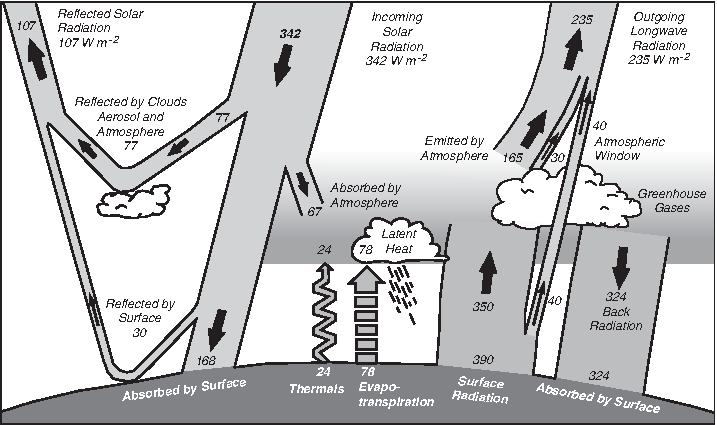
\includegraphics{pics/heatbudget}}
\centering
\footnotesize
Figure 5.6 The mean \rule{0mm}{4ex}annual radiation and heat balance
of the earth. \\After Houghton et al. (1996: 58), which used data from
Kiehl and Trenberth (1996).
\label{fig:heatbudget}
\vspace{-2ex}
\end{figure}

Note that only 20\% of insolation\index{insolation!absorption of}
reaching earth is absorbed directly by the atmosphere while 49\% is
absorbed by the ocean and land. What then warms the atmosphere and
drives the atmospheric circulation? The answer is rain and infrared
radiation from the ocean absorbed by the moist tropical
atmosphere. Here's what happens. Sunlight warms the tropical ocean
which evaporates water to keep from warming up. The ocean also
radiates heat to the atmosphere, but the net radiation term is smaller
than the evaporative term. Trade winds carry the heat in the form of
water vapor to the tropical convergence zone. There the vapor
condenses as rain, releasing its latent heat, and heating the
atmosphere by as much as 125 W/m$^2$ averaged over a year (See figure
14.1).

\begin{figure}[b!]
\vspace{-2ex}
\makebox [121 mm] [c] {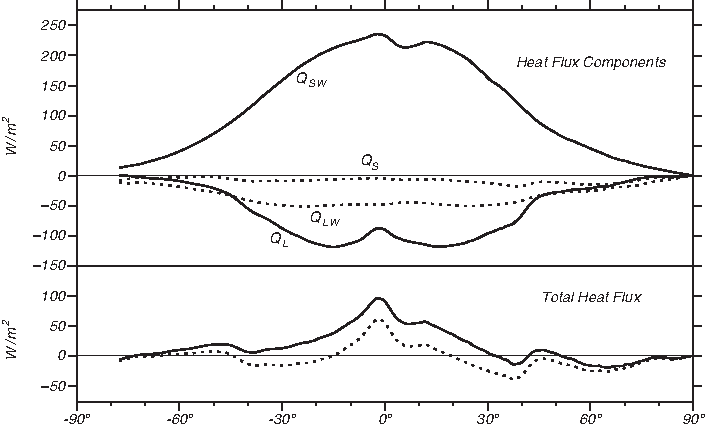
\includegraphics{pics/zonalaveheat}}
\footnotesize
Figure 5.7 \textbf{Upper:} Zonal averages \rule{0mm}{4ex}of heat
transfer to the ocean by insolation\index{insolation!zonal average}
$Q_{SW}$, and loss by infrared radiation $Q_{LW}$, sensible heat
flux\index{sensible heat flux!zonal average} $Q_S$, and latent heat
flux $Q_L$, calculated by DaSilva, Young, and Levitus (1995) using the
\textsc{icoads} data set.  \textbf{Lower:} Net heat flux through the
sea surface calculated from the data above (solid line) and net heat
flux\index{heat flux!zonal average} constrained to give heat and other
transports that match independent calculations of these
transports. The area under the lower curves ought to be zero, but it
is 16 W/m$^2$ for the unconstrained case and -3 W/m$^2$ for the
constrained case.
\label{fig:zonalaveheat}
%\vspace{-3ex}
\end{figure}

At first it may seem strange that rain heats the air. After all, we
are familiar with summertime thunderstorms cooling the air at ground
level. The cool air from thunderstorms is due to downdrafts. Higher in
the cumulus cloud, heat released by rain warms the mid-levels of the
atmosphere causing air to rise rapidly in the storm. Thunderstorms are
large heat engines converting the energy of latent heat into kinetic
energy of winds.

The zonal average of the oceanic heat-budget terms (figure 5.7) shows
that insolation\index{insolation!zonal average} is greatest in the
tropics, that evaporation balances
insolation\index{insolation!balanced by evaporation}, and that
sensible heat flux\index{sensible heat flux!zonal average} is small.
\textit{Zonal average}\index{heat budget!zonal average|textbf} is an
average along lines of constant latitude. Note that the terms in
figure 5.7 don't sum to zero. The areal-weighted integral of the curve
for total heat flux\index{heat flux!global average} is not
zero. Because the net heat flux\index{heat flux!global average} into
the ocean averaged over several years must be less than a few watts
per square meter, the non-zero value must be due to errors in the
various terms in the heat budget.

\begin{figure}[t!]
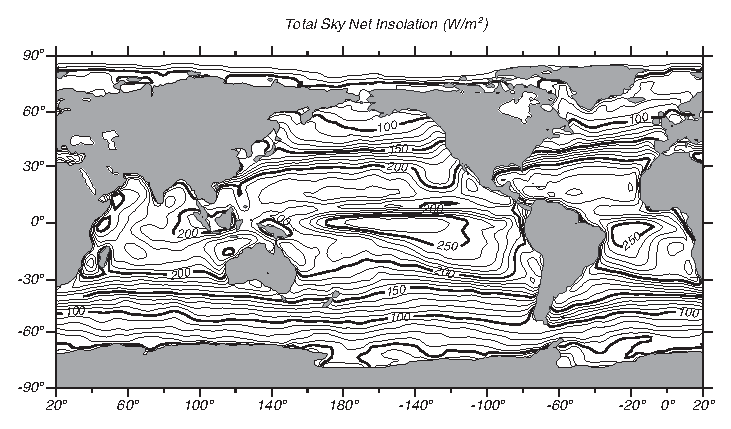
\includegraphics{pics/globalsw}
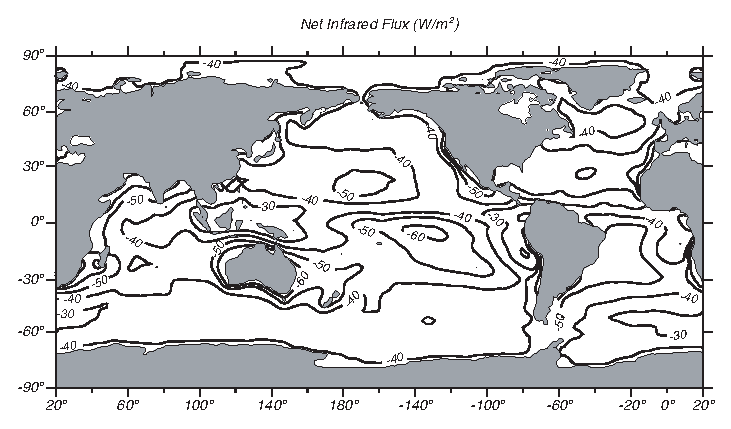
\includegraphics{pics/globalLW}
\footnotesize
Figure 5.8 \rule{0mm}{3ex}Annual-mean
insolation\index{insolation!annual average} $Q_{SW}$ (\textbf{top})
and infrared radiation $Q_{LW}$ (\textbf{bottom}) through the sea
surface during 1989 calculated by the Satellite Data Analysis Center
at the \textsc{nasa} Langley Research Center (Darnell et al., 1992)
using data from the International Satellite Cloud Climatology
Project. Units are W/m$^2$, contour interval is 10 W/m$^2$.
\label{fig:globalSW}
\vspace{-4ex}
\end{figure}

Errors in the heat budget terms can be reduced by using additional
information. For example, we know roughly how much heat and other
quantities are transported\index{transport!heat} by the ocean and
atmosphere, and the known values for these transports can be used to
constrain the calculations of net heat fluxes\index{heat flux!net}
(figure 5.7). The constrained fluxes show that the heat gained by the
ocean in the tropics is balanced by heat lost by the ocean at high
latitudes.

\begin{figure}[t!]
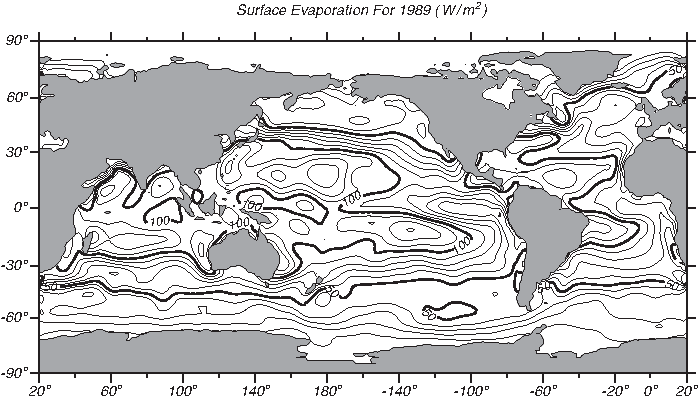
\includegraphics{pics/globallatent}
\footnotesize
Figure 5.9 \rule{0mm}{3ex}Annual-mean latent heat flux\index{heat
  flux!mean annual} from the sea surface $Q_{L}$ in W/m$^2$ during
1989 calculated from data compiled by the Data Assimilation\index{data
  assimilation} Office of \textsc{nasa}'s Goddard Space Flight Center
using reanalyzed data from the \textsc{ecmwf} numerical weather
prediction model. Contour interval is 10 W/m$^2$.
\label{fig:globallatent}
\vspace{-3ex}
\end{figure}

\begin{figure}[t!]
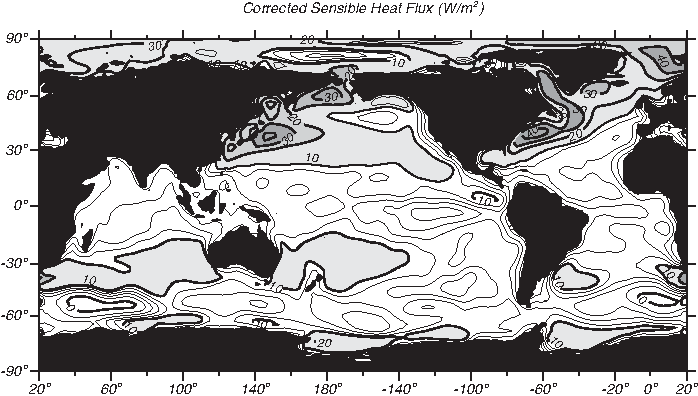
\includegraphics{pics/globalsensible}
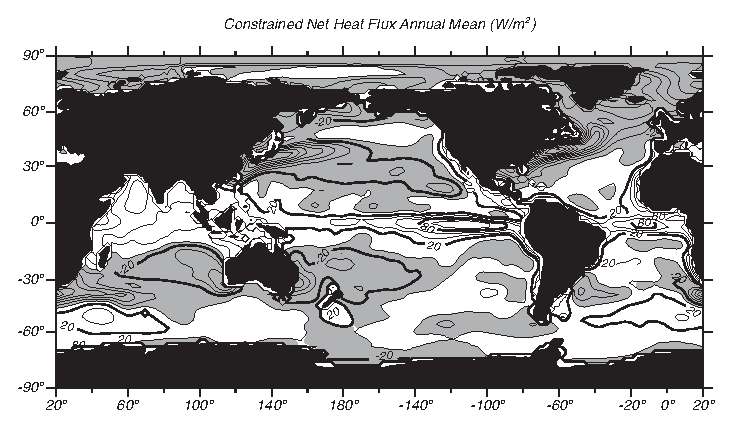
\includegraphics{pics/globalflux}
\footnotesize
Figure 5.10 \rule{0mm}{3ex}Annual-mean upward sensible heat
flux\index{sensible heat flux!annual average} $Q_{S}$ (\textbf{top})
and constrained, net, downward heat flux (\textbf{bottom}) through the
sea surface in W/m$^2$ calculated by DaSilva, Young, and Levitus
(1995) using the \textsc{icoads} data set from 1945 to 1989. Contour
interval is 2 W/m$^2$ (top) and 20 W/m$^2$ (bottom).
\label{fig:globalsensible}
\vspace{-5ex}
\end{figure}

Maps of the regional distribution of fluxes give clues to the
processes producing the fluxes. Clouds regulate the amount of sunlight
reaching the sea surface (figure 5.8 top), and solar heating is
everywhere positive.  The net infrared heat flux\index{infrared flux}
(figure 5.8 bottom) is largest in regions with the least clouds, such
as the center of the ocean and the eastern central Pacific. The net
infrared flux is everywhere negative. Latent heat fluxes (figure 5.9)
are dominated by evaporation in the trade wind regions and the
offshore flow of cold air masses behind cold fronts in winter offshore
of Japan and North America.  Sensible heat fluxes\index{sensible heat
  flux!maps of} (figure 5.10 top) are dominated by cold air blowing
off continents. The net heating gain (figure 5.10 bottom) is largest
in equatorial regions and net heat loss is largest downwind on Asia
and North America.

Heat fluxes change substantially from year to year, especially in the
topics, especially due to El Ni\~{n}o. See Chapter 14 for more on
tropical variability.

\section{Meridional Heat Transport}
\index{meridional transport|textbf}\index{heat
  transport!meridional|textbf}\index{transport!meridional} Overall,
earth gains heat at the top of the tropical atmosphere, and it loses
heat at the top of the polar atmosphere. The atmospheric and oceanic
circulation together must transport heat from low to high latitudes to
balance the gains and losses. This north-south transport is called the
\textit{meridional heat transport}\index{heat transport!meridional}.

The sum of the meridional heat transport in the ocean and atmosphere
is calculated from the zonal average of the net heat flux\index{heat
  flux!net through the top of atmosphere} through the top of the
atmosphere measured by satellites. In making the calculation, we
assume that transports averaged over a few years are steady. Thus any
long-term, net heat gain or loss through the top of the atmosphere
must be balanced by a meridional transport and not by heat
storage\index{heat storage} in the ocean or atmosphere.

\paragraph{Net Heat Flux at the Top of the Atmosphere}
\index{heat budget!through the top of the atmosphere}Heat flux through
the top of the atmosphere is measured very accurately by radiometers
on satellites.
\begin{enumerate}

\vitem
Insolation is calculated from the solar constant\index{solar
  constant!and insolation} and observations of reflected sunlight made
by meteorological satellites and by special satellites of the Earth
Radiation Budget Experiment.

\vitem
Infrared radiation is measured by infrared radiometers on the
satellites.

\vitem
The difference between insolation\index{insolation!at top of
  atmosphere} and net infrared radiation is the net heat
flux\index{heat flux!net through the top of atmosphere} across the top
of the atmosphere.
\end{enumerate}

\paragraph{Net Meridional Heat Transport}
To calculate the meridional heat transport\index{transport!meridional}
in the atmosphere and the ocean, we first average the net heat
flux\index{heat flux!net through the top of atmosphere} through the
top of the atmosphere in a zonal band. Because the meridional
derivative of the transport is the zonal-mean flux, we calculate the
transport from the meridional integral of the zonal-mean flux. The
integral must be balanced by the heat transported by the atmosphere
and the ocean across each latitude band.

Calculations by Trenberth and Caron (2001) show that the total,
annual-mean, meridional heat transport\index{transport!meridional} by
the ocean and atmosphere peaks at 6 PW toward each pole at
35\degrees\ latitude.

\paragraph{Oceanic Heat Transport}
\index{heat transport!calculation of}The meridional heat
transport\index{transport!meridional} in the ocean can be calculated
three ways:
\begin{enumerate}

\vitem
\textit{Surface Flux Method} \index{heat transport!calculation
  of!surface flux method|textbf}calculates the heat flux\index{heat
  flux!net} through the sea surface from measurements of wind,
insolation\index{insolation}, air, and sea temperature, and
cloudiness. The fluxes are integrated to obtain the zonal average of
the heat flux\index{heat flux!zonal average} (figure 5.7). Finally, we
calculate the transport from the meridional integral of the zonal-mean
flux just as we did at the top of the atmosphere.

\vitem
\textit{Direct Method} \index{heat transport!calculation of!direct
  method|textbf} calculates the heat transport from values of current
velocity and temperature measured from top to bottom along a zonal
section spanning an ocean basin. The flux is the product of northward
velocity and heat content derived from the temperature measurement.

\vitem
\textit{Residual Method} \index{heat transport!calculation of!residual
  method|textbf} \index{transport!heat}first calculates the
atmospheric heat transport from atmospheric measurements or the output
of numerical weather models. This is the direct method applied to the
atmosphere. The atmospheric transport is subtracted from the total
meridional transport calculated from the top-of-the-atmosphere heat
flux\index{heat flux!net through the top of atmosphere} to obtain the
oceanic contribution as a residual (figure 5.11).
\end{enumerate}

\begin{figure}[t!]
\makebox [120mm][c]{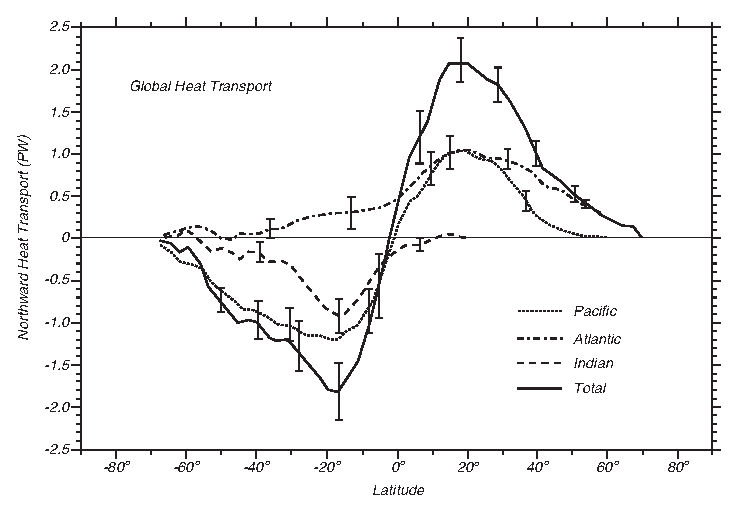
\includegraphics{pics/heattransport}}
\footnotesize
Figure 5.11 Northward \rule{0mm}{3ex}heat
transport\index{transport!heat} for 1988 in each ocean and the total
transport summed over all ocean calculated by the residual method
using atmospheric heat transport from \textsc{ecmwf} and top of the
atmosphere heat fluxes\index{heat flux!net through the top of
  atmosphere} from the Earth Radiation Budget Experiment
satellite. After Houghton et al. (1996: 212), which used data from
Trenberth and Solomon (1994). 1 PW $=$ 1 petawatt $= 10^{15}$ W.
\label{fig:heattransport}
\vspace{-4ex}
\end{figure}
\begin{figure}[b!]
\vspace{-5ex}
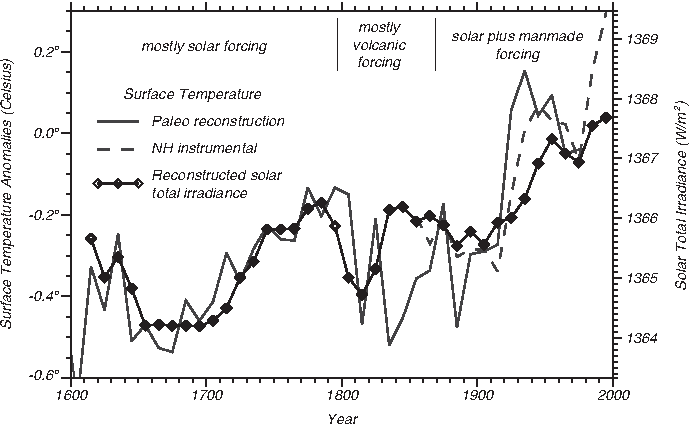
\includegraphics{pics/solarinfluence}
\footnotesize
Figure 5.12 Changes in \rule{0mm}{3ex}solar constant\index{solar
  constant!variability of} (total solar irradiance) and global mean
temperature of earth's surface over the past 400 years. Except for a
period of enhanced volcanic activity in the early 19th century,
surface temperature is well correlated with solar variability. After
Lean, personal communication.
\label{fig:solarinfluence}
%\vspace{-3ex}
\end{figure}

Various calculations of oceanic heat transports,
\index{transport!heat}such as those shown in figure 5.11, tend to be
in agreement, and the error bars shown in the figure are realistic.
The total meridional transport of heat by the ocean is small compared
with the total meridional heat transport by the atmosphere except in
the tropics. At 35\degrees, where the total meridional heat transport
is greatest, the ocean carries only 22\% of the heat in the northern
hemisphere, and 8\% in the southern (Trenberth and Caron, 2001).


\section{Variations in Solar Constant}
\index{solar constant!variability of}We have assumed so far that the
solar constant, the output of light and heat from the sun, is
steady. Recent evidence based on variability of sunspots and faculae
(bright spots) shows that the output varied by $\pm 0.2$\% over
centuries (Lean, Beer, and Bradley, 1995), and that this variability
is correlated with changes in global mean temperature of earth's
surface of $\pm 0.4$\degrees{C}.  (figure 5.12). In addition, White
and Cayan (1998) found a small 12 yr, 22 yr, and longer-period
variations of sea-surface temperature measured by
bathythermographs\index{bathythermograph (BT)} and ship-board
thermometers over the past century. The observed response of earth to
solar variability is about that calculated from numerical models of
the coupled ocean-atmosphere climate system. Many other changes in
climate and weather have been attributed to solar variability. The
correlations are somewhat controversial, and much more information can
be found in Hoyt and Schatten's (1997) book on the subject.

\section{Important Concepts}
\begin{enumerate}
\item Sunlight is absorbed primarily in the tropical ocean. The amount
of sunlight changes with season, latitude, time of day, and cloud
cover.

\vitem Most of the heat absorbed by the ocean in the tropics is
released as water vapor which heats the atmosphere when water is
condenses as rain. Most of the rain falls in the tropical convergence
zones, lesser amounts fall in mid-latitudes near the polar front.

\vitem Heat released by rain and absorbed infrared radiation from the
ocean are the primary drivers for the atmospheric circulation.

\vitem The net heat flux\index{heat flux!net} from the ocean is
largest in mid-latitudes and offshore of Japan and New England.

\vitem Heat fluxes can be measured directly using fast response
instruments on low-flying aircraft, but this is not useful for
measuring heat fluxes\index{heat flux!measurement of} over large
oceanic regions.

\vitem Heat fluxes through large regions of the sea surface can be
calculated from bulk formula. Seasonal, regional, and global maps of
fluxes are available based on ship and satellite observations.

\vitem The most widely used data sets for studying heat
fluxes\index{heat flux!from \textsc{icoads}} are the International
Comprehensive Ocean-Atmosphere Data Set and the reanalysis of
meteorological data by numerical weather prediction models.

\vitem The atmosphere transports most of the
heat\index{transport!heat} needed to warm latitudes higher than
35\degrees. The oceanic meridional transport is comparable to the
atmospheric meridional transport only in the tropics.

\vitem Solar output is not constant, and the observed small variations
in output of heat and light from the sun seem to produce the changes
in global temperature observed over the past 400 years.
\end{enumerate}


\chapter{Temperature, Salinity, and Density}
Heat fluxes, evaporation, rain, river inflow, and freezing and melting of sea
ice all influence the distribution of temperature and salinity at the ocean's
surface. Changes in temperature and salinity can increase or decrease the density
of water at the surface, which can lead to convection. If water from the
surface sinks into the deeper ocean, it retains a distinctive relationship between
temperature and salinity which helps oceanographers track the movement of deep
water. In addition, temperature, salinity, and pressure are used to calculate
density. The distribution of density inside the ocean is directly related to the
distribution of horizontal pressure gradients and ocean currents.  For all these
reasons, we need to know the distribution of temperature, salinity, and density in
the ocean.

Before discussing the distribution of temperature and salinity, let's first define
what we mean by the terms, especially salinity.

\section{Definition of Salinity}
At the simplest level, salinity\index{salinity|textbf} is the total
amount of dissolved material in grams in one kilogram of sea
water. Thus salinity is a dimensionless quantity. It has no units. The
variability of dissolved salt is very small, and we must be very
careful to define salinity in ways that are accurate and practical. To
better understand the need for accuracy\index{accuracy!salinity}, look
at figure 6.1. Notice that the range of salinity for most of the
ocean's water is from 34.60 to 34.80 parts per thousand, which is 200
parts per million. The variability in the deep North Pacific is even
smaller, about 20 parts per million. If we want to classify water with
different salinity, we need definitions and instruments accurate to
about one part per million. Notice that the range of temperature is
much larger, about 1\degrees{C}, and temperature is easier to measure.

Writing a practical definition of salinity that has useful accuracy is
difficult (see Lewis, 1980, for the details), and various definitions
have been used.\\

\begin{figure}[t!]
\makebox [120mm][c]{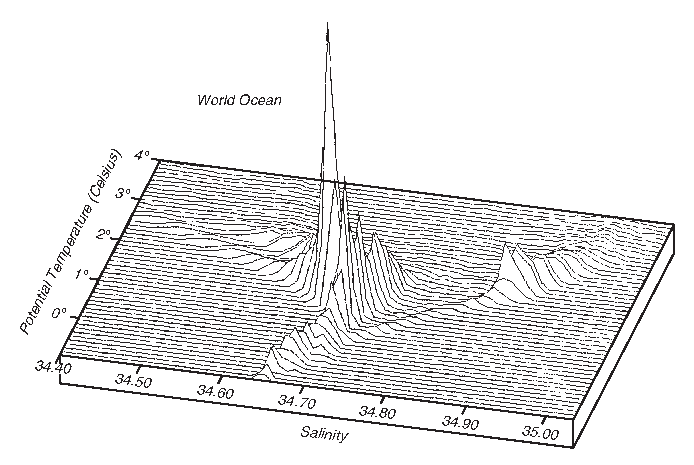
\includegraphics{pics/salhistogram}}
\footnotesize
Figure 6.1 Histogram of temperature \rule{0mm}{3ex}and salinity of
ocean water colder than 4\degrees C. Height is proportional to
volume. Height of highest peak corresponds to a volume of 26 million
cubic kilometers per bivariate class of 0.1\degrees{C} and 0.01. After
Worthington (1981: 47).
\label{fig:salhistogram}
\vspace{-3ex}
\end{figure}

\paragraph{A Simple Definition}
Originally salinity was defined to be the
``Total\index{salinity|textbf} amount of dissolved material in grams
in one kilogram of sea water.'' This is not useful because the
dissolved material is almost impossible to measure in practice. For
example, how do we measure volatile material like gasses? Nor can we
evaporate sea-water to dryness because chlorides are lost in the last
stages of drying (Sverdrup, Johnson, and Fleming, 1942: 50).

\paragraph{A More Complete Definition}
To avoid these difficulties, the \index{salinity!simple
  vs. complete}International Council for the Exploration of the Sea
set up a commission in 1889 which recommended that salinity be defined
as the ``Total amount of solid materials in grams dissolved in one
kilogram of sea water when all the carbonate has been converted to
oxide, the bromine and iodine replaced by chlorine and all organic
matter completely oxidized.'' The definition was published in
1902. \textit{This is useful but difficult to use routinely}.

\paragraph{Salinity Based on Chlorinity}
Because the above definition was difficult \index{salinity!based on
  chlorinity}to implement in practice, because salinity is directly
proportional to the amount of chlorine in sea water, and because
chlorine can be measured accurately by a simple chemical analysis,
salinity $S$ was redefined using chlorinity:
\begin{equation}
S = 0.03 + 1.805\, Cl
\end{equation}
where \textit{chlorinity}\index{chlorinity|textbf} $Cl$ is defined as
``the mass of silver required to precipitate completely the halogens
in 0.328 523 4 kg of the sea-water sample.''

As more and more accurate measurements were made, (6.1) turned out to
be too inaccurate. In 1964 \textsc{unesco} and other international
organizations appointed a Joint Panel on Oceanographic Tables and
Standards to produce a more accurate definition. The Joint Panel
recommended in 1966 (Wooster, Lee, and Dietrich, 1969) that salinity
and chlorinity be related using:
\begin{equation}
S = 1.806\,55\,Cl
\end{equation}
This is the same as (6.1) for $S=35$.

\paragraph{Salinity Based on Conductivity}
At the same time (6.2) was \index{salinity!based on
  conductivity}adopted, ocean\-ographers had began using conductivity
meters to measure salinity. The meters were very precise and
relatively easy to use compared with the chemical techniques used to
measure chlorinity. As a result, the Joint Panel also recommended that
salinity be related to conductivity\index{conductivity} of sea water
using:
\begin{subequations}
\begin{align}
S  = &-0.089\,96 + 28.297\,29\,R_{15} + 12.808\,32\,R^2_{15} \notag \\
&-10.678\,69\,R^3_{15} + 5.986\,24\,R^4_{15} - 1.323\,11\,R^5_{15} \\
R_{15} = \: &C(S,15,0)/C(35,15,0)
\end{align}
\end{subequations}
where $C(S, 15, 0)$ is the conductivity of the sea-water sample at
15\degrees C and atmospheric pressure, having a salinity $S$ derived
from (6.4), and $C(35, 15, 0)$ is the conductivity of standard
``Copenhagen'' sea water\index{Copenhagen sea water}. Millero (1996)
points out that (6.3) is not a new definition of salinity, it merely
gives chlorinity as a function of conductivity of seawater relative to
standard seawater.

\paragraph{Practical Salinity Scale of 1978}
By the early 1970s, accurate conductivity meters could be deployed
from ships to measure conductivity at depth. The need to re-evaluate
the salinity scale led the Joint Panel to recommend in 1981
(\textsc{jpots}, 1981; Lewis, 1980) that salinity be defined using
only conductivity, breaking the link with chlorinity. All water
samples with the same conductivity ratio have the same salinity even
though the their chlorinity may differ.

The \textit{Practical Salinity Scale of 1978}\index{salinity!Practical
  Salinity Scale|textbf} is now the official definition:
\begin{subequations}
\begin{align}
S       = &\:0.0080  -0.1692\,K^{1/2}_{15} + 25.3851\,K_{15} + 14.0941\,K^{3/2}_{15} \notag \\
          &- 7.0261\,K^{2}_{15} + 2.7081\,K^{5/2}_{15} \\
K_{15}  = &\:C(S,15,0)/C(KCl,15,0) \\
2 \leq S &\:\leq 42 \notag
\end{align}
\end{subequations}
where $C(S, 15, 0)$ is the conductivity of the sea-water sample at a
temperature of 14.996\degrees C on the International Temperature Scale
of 1990 (\textsc{its}-90, see \S 6.2) and standard atmospheric
pressure of 101 325 Pa\index{pressure!standard atmospheric}.
$C(KCl, 15, 0)$ is the conductivity of the standard potassium chloride (KCl)
solution at a temperature of 15\degrees C and standard atmospheric
pressure. The standard KCl solution contains a mass of $32.435\,6$
grams of KCl in a mass of $1.000\,000$ kg of solution. Millero (1996:
72) and Lewis (1980) gives equations for calculating salinity at other
pressures and temperatures.

\paragraph{Comments}
The various definitions of salinity work well because the ratios of
the various ions in sea water are nearly independent of salinity and
location in the ocean (table 6.1). Only very fresh waters, such as are
found in estuaries, have significantly different ratios. The result is
based on Dittmar's (1884) chemical analysis of 77 samples of sea water
collected by the \textit{Challenger} Expedition and further studies by
Carritt and Carpenter (1959).
\begin{quote} \small
The importance of this result cannot be over emphasized, as upon it
depends the validity of the chlorinity: salinity: density
relationships and, hence, the accuracy\index{accuracy!density} of all
conclusions based on the distribution of density where the latter is
determined by chemical or indirect physical methods such as electrical
conductivity$\ldots$---Sverdrup, Johnson, Fleming (1942).
\end{quote}
The relationship between conductivity and salinity has an
accuracy\index{accuracy!salinity} of around $\pm 0.003$ in
salinity. The very small error is caused by variations in constituents
such as SiO$_2$ which cause small changes in density but no change in
conductivity.

\begin{table}[h!]\centering \small
\begin{tabular*}{72mm}{@{}clcl@{}}
\multicolumn{4}{@{}l@{}}{\bfseries Table 6.1 Major \rule[-1ex]{0mm}{1ex}Constituents of Sea Water} \\
\hline
 & Ion & & \rule{0ex}{2.5ex}Atoms \\
\hline
55.3\% & \rule{0ex}{2.5ex}Chlorine & 55.3\% & Chlorine \\
30.8\% & Sodium & 30.8\% & Sodium \\
7.7\%  & Sulfate & 3.7\% & Magnesium \\
3.7\%  & Magnesium & 2.6\% & Sulfur \\
1.2\%  & Calcium & 1.2\% & Calcium \\
1.1\%  & Potassium & 1.1\% & Potassium \\[0.5ex]
\hline
\end{tabular*} \\[0.5ex]
\vspace{-3ex}
\end{table}

\paragraph{Reference Seawater and Salinity}
The Practical Salinity Scale of 1978 introduced several small
problems. It led to confusion about units and to the use of
``practical salinity units" that are not part of the definition of
Practical Salinity. In addition, absolute salinity differs from
salinity by about 0.5\%. And, the composition of seawater differs
slightly from place to place in the ocean, leading to small errors in
measuring salinity.

To avoid these and other problems, Millero et al (2008) defined a new
measure of salinity, the Reference Salinity, that accurately
represents the Absolute Salinity of an artificial seawater
solution. It is based on a Reference Composition of seawater that is
much more accurate than the values in Table 6.1 above. The
\textit{Reference Composition}\index{salinity!Reference|textbf} of the
artificial seawater is defined by a list of solutes and their mole
fractions given in Table 4 of their paper. From this, they defined
artificial \textit{Reference Seawater}\index{Reference
  Seawater|textbf} to be seawater having a Reference Composition
solute dissolved in pure water as the solvent, and adjusted to its
thermodynamic equilibrium state. Finally, the \textit{Reference
  Salinity} of Reference Seawater was defined to be exactly 35.16504 g
kg$^{-1}$.

With these definitions, plus many details described in their paper,
Millero et al (2008) show Reference Salinity is related to Practical
Salinity\index{salinity!practical} by:
\begin{equation}
S_R \approx (35.16504/35) \text{g kg}^{-1} \times S
\end{equation}
The equation is exact at $S = $ 35. Reference Salinity is
approximately 0.47\% larger than Practical Salinity. Reference
Salinity $S_R$ is intended to be used as an SI-based extension of
Practical Salinity.

\section{Definition of Temperature}
\index{temperature|textbf}Many physical processes depend on
temperature.\index{temperature} A few can be used to define absolute
temperature $T$. The unit of $T$ is the kelvin, which has the symbol
K. The fundamental processes used for defining an absolute temperature
scale over the range of temperatures found in the ocean include
(Soulen and Fogle, 1997): 1) the gas laws relating pressure to
temperature of an ideal gas with corrections for the density of the
gas; and 2) the voltage noise of a resistance $R$.

The measurement of temperature using an absolute
scale\index{temperature!absolute} is difficult and the measurement is
usually made by national standards laboratories. The absolute
measurements are used to define a practical temperature
scale\index{temperature!practical scale} based on the temperature of a
few fixed points and interpolating devices which are calibrated at the
fixed points.

For temperatures commonly found in the ocean, the interpolating device
is a platinum-resistance thermometer. It consists of a loosely wound,
strain-free, pure platinum wire whose resistance is a function of
temperature. It is calibrated at fixed points between the triple point
of equilibrium hydrogen at 13.8033 K and the freezing point of silver
at 961.78 K, including the triple point of water at 0.060\degrees C,
the melting point of Gallium at 29.7646\degrees C, and the freezing
point of Indium at 156.5985\degrees C (Preston-Thomas, 1990). The
triple point of water is the temperature at which ice, water, and
water vapor are in equilibrium. The temperature scale in kelvin $T$ is
related to the temperature scale in degrees Celsius $t$[\degrees C]
by:
\begin{equation}
t \text{ [\degrees C]} = T \text{ [K]} -273.15
\end{equation}

\begin{figure}[t!]
%\vspace{-4ex}
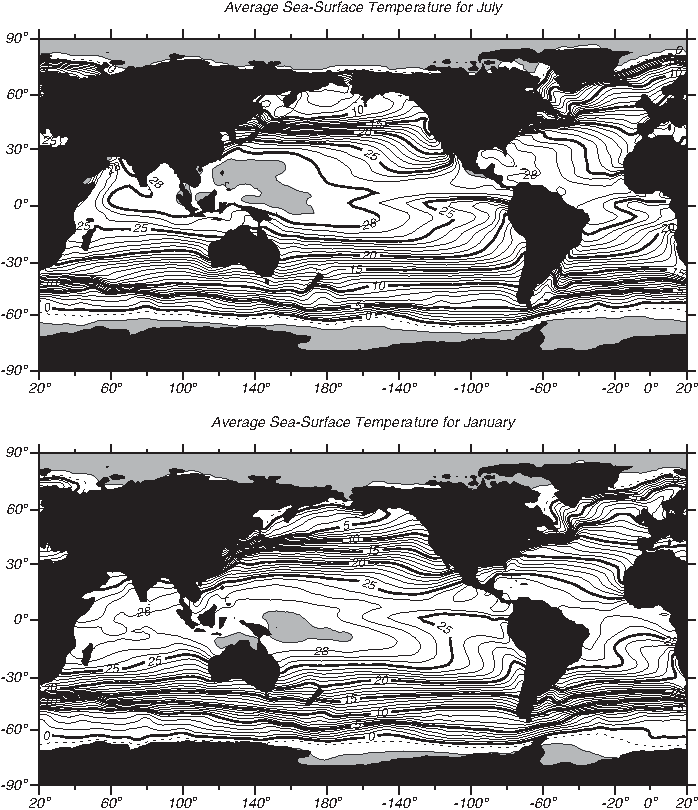
\includegraphics{pics/sst_climatology}
\footnotesize
Figure 6.2 Mean sea-surface \rule{0mm}{3ex}temperature calculated from
the optimal interpolation technique (Reynolds and Smith, 1995) using
ship reports and \textsc{avhrr} measurements of temperature. Contour
interval is 1\degrees C with heavy contours every 5\degrees C. Shaded
areas exceed 29\degrees C.
\label{fig:sst_climatology}
\vspace{-4ex}
\end{figure}

The practical temperature scale was revised in 1887, 1927, 1948, 1968,
and 1990 as more accurate determinations of absolute temperature
became accepted. The most recent scale is the International
Temperature Scale of 1990
(\textsc{its}-90)\index{temperature!International Temperature
  Scale}. It differs slightly from the International Practical
Temperature Scale of 1968 \textsc{ipts}-68. At 0\degrees C they are
the same, and above 0\degrees C \textsc{its}-90 is slightly
cooler. $t_{90}-t_{68} = -0.002$ at 10\degrees C, $-0.005$ at
20\degrees C, $-0.007$ at 30\degrees C and $-0.010$ at 40\degrees C.

\begin{figure}[b!]
\vspace{-3ex}
\makebox[121mm][c]{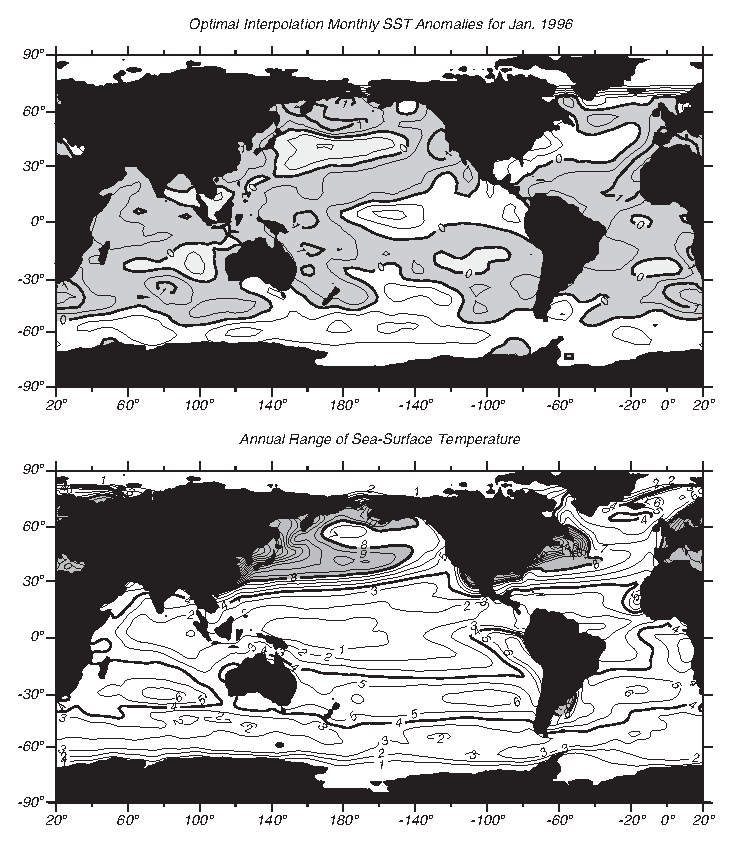
\includegraphics{pics/SSTvariability}}
\footnotesize
Figure 6.3 \textbf{Top:} Sea-surface \rule{0mm}{3ex}temperature
anomaly for January 1996 relative to mean temperature shown in figure
6.2 using data published by Reynolds and Smith (1995) in the
\textit{Climate Diagnostics Bulletin} for February 1995. Contour
interval is 1\degrees C. Shaded areas are
positive. \textbf{Bottom:}Annual range of sea-surface temperature in
\degrees{C} calculated from the Reynolds and Smith (1995) mean
sea-surface temperature data set. Contour interval is 1\degrees C with
heavy contours at 4\degrees C and 8\degrees C. Shaded areas exceed
8\degrees C.
\label{fig:SSTvariability}
%\vspace{-3ex}
\end{figure}

Notice that while oceanographers use thermometers calibrated with an
accuracy\index{accuracy!temperature} of a millidegree, which is
0.001\degrees C, the temperature scale itself has uncertainties of a
few millidegrees.

\section[Geographical Distribution]{Geographical Distribution of Surface
Temperature and Salinity} \index{salinity!geographical distribution
  of}\index{temperature!geographical distribution of}The distribution
of temperature at the sea surface tends to be \textit{zonal},
\index{zonal|textbf}that is, it is independent of longitude (figure
6.2). Warmest water is near the equator, coldest water is near the
poles. The deviations from zonal are small. Equatorward of 40\degrees,
cooler waters tend to be on the eastern side of the basin. North of
this latitude, cooler waters tend to be on the western side.

The \textit{anomalies} \index{anomalies!sea-surface
  temperature|textbf}of sea-surface temperature, the deviation from a
long term average, are small, less than 1.5\degrees C (Harrison and
Larkin, 1998) except in the equatorial Pacific where the deviations
can be 3\degrees{C} (figure 6.3: top).

\begin{figure}[t!]
\makebox[121mm][c]{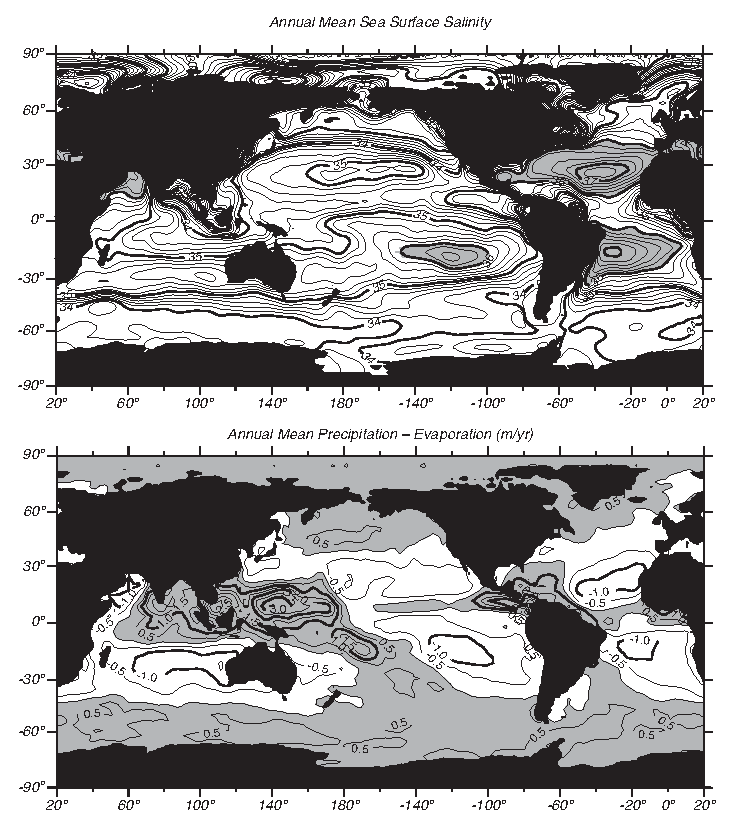
\includegraphics{pics/salinity}}
\footnotesize
Figure 6.4 \textbf{Top}: Mean sea-surface \rule{0pt}{3ex}
salinity. \rule{0mm}{2ex}Contour interval is 0.25. Shaded areas exceed
a salinity of 36. From Levitus (1982).  \textbf{Bottom}: Precipitation
minus evaporation in meters per year calculated from global
rainfall\index{rainfall!global} by the Global Precipitation
Climatology Project and latent heat flux calculated by the Data
Assimilation Office, both at \textsc{nasa}'s Goddard Space Flight
Center. Precipitation exceeds evaporation in the shaded regions,
contour interval is 0.5 m.

\label{fig:salinity}
\vspace{-3ex}
\end{figure}

The annual range of surface temperature is highest at mid-latitudes,
especially on the western side of the ocean (figure 6.3: bottom). In
the west, cold air blows off the continents in winter and cools the
ocean. The cooling dominates the heat budget. In the tropics the
temperature range is mostly less than 2\degrees{C}.

The distribution of sea-surface salinity also tends to be zonal. The
saltiest waters are at mid-latitudes where evaporation is high. Less
salty waters are near the equator where rain freshens the surface, and
at high latitudes where melted sea ice freshens the surface (figure
6.4). The zonal (east-west) average of salinity shows a close
correlation between salinity and evaporation minus precipitation plus
river input (figure 6.5).

Because many large rivers drain into the Atlantic and the Arctic Sea,
why is the Atlantic saltier than the Pacific? Broecker (1997) showed
that 0.32 Sv of the water evaporated from the Atlantic does not fall
as rain on land. Instead, it is carried by winds into the Pacific
(figure 6.6). Broecker points out that the quantity is small,
equivalent to a little more than the flow in the Amazon River, but
``were this flux not compensated by an exchange of more salty Atlantic
waters for less salty Pacific waters, the salinity of the entire
Atlantic would rise about 1 gram per liter per millennium.''

\begin{figure}[t!]
%\vspace{-2ex}
\makebox [121mm][c]{\includegraphics{pics/zonalsalinity}}
\footnotesize
Figure 6.5 Zonal average of sea-surface \rule{0mm}{3ex}salinity
calculated for all the ocean from Levitus (1982) and the difference
between evaporation and precipitation ($E - P$) calculated from data
shown in figure 6.4 (bottom).
\label{fig:zonalsalinity}
\vspace{-5ex}
\end{figure}

\begin{figure}[b!]
\vspace{-3ex}
\makebox[121mm][c]{\includegraphics{pics/BroeckerPlot}}
\footnotesize
Figure 6.6 Water \rule{0pt}{3ex} transported
\index{transport!atmospheric}by the atmosphere into and out of the
Atlantic. Basins draining into the Atlantic are black, deserts are
white, and other drainage basins are shaded. Arrows give direction of
water transport by the atmosphere, and values are in Sverdrups. Bold
numbers give the net transport for the Atlantic at each latitude
band. Overall, the Atlantic loses 0.32 Sv, an amount approximately
equal to the flow in the Amazon River. After Broecker (1997).
\label{fig:BroeckerPlot}
%\vspace{-4ex}
\end{figure}

\begin{figure}[t!]
%\vspace{-2ex}
\makebox[121 mm][c]{\includegraphics{pics/seasonalthermo}}
\footnotesize
Figure 6.7 Growth and decay \rule{0mm}{4ex} of the mixed
layer\index{mixed layer!seasonal growth and decay} and seasonal
thermocline\index{thermocline!seasonal} from November 1989 to
September 1990 at the Bermuda Atlantic Time-series Station
(\textsc{bats}) at 31.8\degrees N 64.1\degrees W. Data were collected
by the Bermuda Biological Station for Research, Inc. Note that
pressure in decibars is nearly the same as depth in meters (see \S 6.8
for a definition of decibars).
\label{fig:seasonalthermo}
\vspace{-4ex}
\end{figure}

\textit{Mean Temperature and Salinity of the Ocean} \index{ocean!mean
  temperature|textbf}\index{ocean!mean salinity|textbf}The mean
temperature of the ocean's waters is: t = 3.5\degrees{C}. The mean
salinity is S = 34.7. The distribution about the mean is small: 50\%
of the water is in the range:
\begin{align}
1.3^{\circ}\text{C} < &\:t < 3.8^{\circ}\text{C} \notag \\
34.6 < &\:S < 34.8 \notag
\end{align}

\section{The Oceanic Mixed Layer and Thermocline}
Wind blowing on the ocean stirs the upper layers leading to a thin
\textit{mixed layer} \index{mixed layer|textbf}at the sea surface
having constant temperature and salinity from the surface down to a
depth where the values differ from those at the surface. The magnitude
of the difference is arbitrary, but typically the temperature at the
bottom of the layer must be no more than 0.02--0.1\degrees\ colder
than at the surface. Note that both temperature and salinity must be
constant in the mixed layer. We will see later that mean velocity is
not constant. The mixed layer is roughly 10--200 m thick over most of
the tropical and mid-latitude belts.

The depth and temperature of the mixed layer\index{mixed
  layer!external forcing of} varies from day to day and from season to
season in response to two processes:
\begin{enumerate}
\vitem Heat fluxes through the surface heat and cool the surface
waters. Changes in temperature change the density contrast between the
mixed layer and deeper waters. The greater the contrast, the more work
is needed to mix the layer downward and visa versa.

\vitem Turbulence in the mixed layer mixes heat downward. The
turbulence\index{turbulence!in mixed layer} depends on the wind speed
and on the intensity of breaking waves. Turbulence mixes water in the
layer, and it mixes the water in the layer with water in the
thermocline\index{thermocline}.
\end{enumerate}

The mid-latitude mixed layer\index{mixed layer!mid-latitude} is
thinnest in late summer when winds are weak, and sunlight warms the
surface layer (figure 6.7). At times, the heating is so strong, and
the winds so weak, that the layer is only a few meters thick. In fall,
the first storms of the season mix the heat down into the ocean
thickening the mixed layer, but little heat is lost. In winter, heat
is lost, and the mixed layer continues to thicken, becoming thickest
in late winter. In spring, winds weaken, sunlight increases, and a new
mixed layer forms.

\begin{figure}[t!]
%\vspace{-2ex}
\makebox[121 mm] [c] {\includegraphics{pics/TandSProfile}}
%\centering
\footnotesize
Figure 6.8 Typical \rule{0mm}{4ex}temperature and salinity profiles in
the open ocean. AAC: At 62.0\degrees\ S, 170.0\degrees\ E in the
Antarctic Circumpolar Current\index{Antarctic Circumpolar Current} on
16 January 1969 as measured by the \textit{R/V Hakuho Maru}. Warm
Pool: At 9.5\degrees\ N 176.3\degrees\ E in the tropical west Pacific
warm pool on 12 March 1989 as measured by Bryden and Hall on the
\textit{R/V Moana Wave}.  \textsc{bats}: At 31.8\degrees\ N
64.1\degrees\ W near Bermuda on 17 April and 10 September 1990 as
measured by the Bermuda Biological Station for Research, Inc.  Data
are included with Java OceanAtlas.
\label{fig:TandSProfile}
\vspace{-5ex}
\end{figure}

Below the mixed layer\index{mixed layer!mid-latitude}, water
temperature decreases rapidly with depth except at high latitudes. The
range of depths where the rate of change, the gradient of temperature,
is large is called the
\textit{thermocline}\index{thermocline|textbf}. Because density is
closely related to temperature, the thermocline also tends to be the
layer where density gradient is greatest, the
\textit{pycnocline}\index{pycnocline|textbf}.

The shape of the thermocline varies slightly with the seasons (figure 6.7).
This is the \textit{seasonal thermocline}.
\index{thermocline!seasonal|textbf} The \textit{permanent thermocline}
\index{thermocline!permanent|textbf}extends from below the seasonal
thermocline to depths of 1500--2000 meters (figure 6.8). At high
latitudes, such as at the \textsc{aac} station in the figure, there
may be a cooler, fresher layer above the permanent thermocline.

The mixed layer tends to be saltier than the
thermocline\index{thermocline} between 10\degrees\ and
40\degrees\ latitude, where evaporation exceeds precipitation. At high
latitudes the mixed layer\index{mixed layer!high latitude} is fresher
because rain and melting ice reduce salinity. In some tropical
regions, such as the warm pool in the western tropical Pacific, rain
also produces a thin fresher mixed layer\index{mixed layer!tropical
  Pacific}.

\section[Density]{Density, Potential Temperature, and Neutral Density}
During winter, cold water formed at the surface sinks to a depth
determined by its density relative to the density of the deeper
water. Currents then carry the water to other parts of the ocean. At
all times, the water parcel moves to stay below less dense water and
above more dense water. The distribution of currents within the ocean
depends on the distribution of pressure, which depends on the
variations of density inside the ocean as outlined in \S10.4. So, if
we want to follow water movement within the ocean, we need to know the
distribution of density within the ocean.

\paragraph{Density and sigma-t}
\index{density}The calculation of water movement requires measurements
of density with an accuracy\index{accuracy!density} of a few parts per
million. This is not easy.

\textit{Absolute Density} \index{density!absolute|textbf}of water can
only be measured in special laboratories, and only with
difficulty. The best accuracy is $1\,:\, 2.5 \times 10^5 = 4$ parts
per million.

To avoid the difficulty of working with absolute density,
oceanographers use density relative to density of pure water. Density
$\rho (S, t, p)$ is now defined using Standard Mean Ocean Water of
known isotopic composition, assuming saturation of dissolved
atmospheric gasses. Here $S, t, p$ refers to salinity, temperature,
and pressure.

In practice, density is not measured, it is calculated from \textit{in
  situ} \index{in situ} measurements of pressure, temperature, and
conductivity using the equation of state for sea water. This can be
done with an accuracy\index{accuracy!density} of two parts per
million.

Density of water at the sea surface is typically 1027 kg/m$^3$. For
simplification, physical oceanographers often quote only the last 2
digits of the density, a quantity they call \textit{density anomaly}
or \textit{Sigma (S,t,p)}\index{density!anomaly or sigma|textbf}:
\begin{equation}
\sigma(S,t,p) = \rho (S, t, p) - 1000 \text{\ kg/m$^3$}
\end{equation}
The Working Group on Symbols, Units and Nomenclature in Physical
Oceanography (\textsc{sun}, 1985) recommends that $\sigma$ be replaced
by $\gamma$ because $\sigma$ was originally defined relative to pure
water and it was dimensionless. Here, however, I will follow common
practice and use $\sigma$.

If we are studying surface layers of the ocean, we can ignore
compressibility, and we use a new quantity sigma-t (written $\sigma_t$):
\begin{equation}
\sigma _t =  \sigma(S,t,0)
\end{equation}
This is the density anomaly of a water sample when the total pressure
on it has been reduced to atmospheric pressure (\textit{i.e.} zero
water pressure), but the temperature and salinity are \textit{in situ}
values.\index{in situ}

\begin{figure}[t!]
\makebox[121 mm] [c] {\includegraphics{pics/thetaprofile}}
\footnotesize
Figure 6.9 Profiles \rule{0mm}{4ex}of \textbf{Left} \textit{in
  situ}\index{in situ} $t$ and potential $\theta$ temperature and
\textbf{Right} sigma-t and sigma-theta in the Kermadec Trench in the
Pacific measured by the R/V Eltanin during the Scorpio Expedition on
13 July 1967 at 175.825\degrees\ E and 28.258\degrees\ S. Data from
Warren (1973).

\label{fig:thetaprofile}
\vspace{-4ex}
\end{figure}

\paragraph{Potential Temperature}
\index{temperature!potential}\index{potential!temperature}As a water
parcel moves within the ocean below the mixed layer\index{mixed
  layer}, its salt and heat content can change only by mixing with
other water. Thus we can use measurements of temperature and salinity
to trace the path of the water. This is best done if we remove the
effect of compressibility.

As water sinks, pressure increases, the water is compressed, and the
compression does work on the water. This increases the internal energy
of the water. To understand how compression increases energy, consider
a cube containing a fixed mass of water. As the cube sinks, its sides
move inward as the cube is compressed. Recalling that work is force
times distance, the work is the distance the side moves times the
force exerted on the side by pressure. The change in internal energy
may or may not result in a change in temperature (McDougall and
Feistel, 2003). The internal energy of a fluid is the sum of molecular
kinetic energy (temperature) and molecular potential energy. In sea
water, the later term dominates, and the change of internal energy
produces the temperature change shown in figure 6.9. At a depth of 8
km, the increase in temperature is almost 0.9\degrees\ C.

To remove the influence of compressibility from measurements of
temperature, oceanographers (and meteorologists who have the same
problem in the atmosphere) use the concept of potential
temperature. \textit{Potential
  temperature}\index{temperature!potential|textbf}\index{potential!temperature|textbf}
$\Theta$ is defined as the temperature of a parcel of water at the sea
surface after it has been raised adiabatically from some depth in the
ocean. Raising the parcel \textit{adiabatically}
\index{adiabatically|textbf}means that it is raised in an insulated
container so it does not exchange heat with its surroundings. Of
course, the parcel is not actually brought to the surface. Potential
temperature is calculated from the temperature in the water at depth,
the \textit{in situ}\index{in situ} temperature.

\paragraph{Potential Density}
\index{density!potential|textbf}\index{potential!density|textbf}If we
are studying intermediate layers of the ocean, say at depths near a
kilometer, we cannot ignore compressibility. Because changes in
pressure primarily influence the temperature of the water, the
influence of pressure can be removed, to a first approximation, by
using the \textit{potential density}.

\textit{Potential density} $\rho _{\Theta}$ is the density a parcel of
water would have if it were raised adiabatically to the surface
without change in salinity. Written as sigma,
\begin{equation}
\sigma _{\Theta} = \sigma(S, \Theta, 0)
\end{equation}
$\sigma _{\Theta}$ is especially useful because it is a conserved
thermodynamic property.

Potential density is not useful for comparing density of water at
great depths. If we bring water parcels to the surface and compare
their densities, the calculation of potential density ignores the
effect of pressure on the coefficients for thermal and salt
expansion. As a result, two water samples having the same density but
different temperature and salinity at a depth of four kilometers can
have noticeably different potential density. In some regions the use
of $\rho(\Theta)$ can lead to an apparent decrease of density with
depth (figure 6.10) although we know that this is not possible because
such a column of water would be unstable.

\begin{figure}[b!]
\vspace{-2ex}
\includegraphics{pics/atlsection}
\footnotesize
Figure 6.10 Vertical \rule{0mm}{4ex}sections of density in the western
Atlantic.  Note that the depth scale changes at 1000 m
depth. \textbf{Upper}: $\sigma _{\Theta}$, showing an apparent density
inversion below 3,000 m. \textbf{Lower}: $\sigma _4$ showing
continuous increase in density with depth. After Lynn and Reid (1968).
\label{fig:atlsection4}
%\vspace{-4ex}
\end{figure}

To compare samples from great depths, it is better to bring both
samples to a nearby depth instead of to the surface $p = 0$. For
example, we can bring both parcels to a pressure of 4,000 decibars,
which is near a depth of 4 km:
\begin{equation}
\sigma_4 = \sigma(S, \Theta, 4000)
\end{equation}
where $\sigma_4$ is the density of a parcel of water brought
adiabatically to a pressure of 4,000 decibars. More generally,
oceanographers sometimes use $\rho_r$
\begin{equation}
\sigma _r = \sigma(S, \Theta, p, p_r)
\end{equation}
where $p$ is pressure, and $p_r$ is pressure at some reference
level. In (6.8) the level is $p_r = 0$ decibars, and in (6.9)
$p_r = 4000$ decibars.

The use of $\sigma_r$ leads to problems. If we wish to follow parcels
of water deep in the ocean, we might use $\sigma_3$ in some areas, and
$\sigma_4$ in others.  But what happens when a parcel moves from a
depth of 3 km in one area to a depth of 4 km in another? There is a
small discontinuity between the density of the parcel expressed as
$\sigma_3$ compared with density expressed as $\sigma_4$. To avoid
this difficulty, Jackett and McDougall (1997) proposed a new variable
they called neutral density.

\paragraph{Neutral Surfaces and Density}
\index{neutral surfaces}\index{density!neutral surfaces}A parcel of
water moves locally along a path of constant density so that it is
always below less dense water and above more dense water. More
precisely, it moves along a path of constant potential density
$\sigma_r$ referenced to the local depth $r$. Such a path is called a
\textit{neutral path}\index{neutral path|textbf} (Eden and Willebrand,
1999). A \textit{neutral surface element} \index{neutral surface
  element|textbf}is the surface tangent to the neutral paths through a
point in the water. No work is required to move a parcel on this
surface because there is no buoyancy\index{buoyancy} force acting on
the parcel as it moves (if we ignore friction).

Now let's follow the parcel as it moves away from a local region. At
first we might think that because we know the tangents to the surface
everywhere, we can define a surface that is the envelope of the
tangents. But an exact surface is not mathematically possible in the
real ocean, although we can come very close.

Jackett and McDougall (1997) developed a practical neutral density
variable $\gamma^n$ and surface that stays within a few tens meters of
an ideal surface anywhere in the world.  They constructed their
variables using data in the Levitus (1982) atlas. The neutral density
values were then used to label the data in the Levitus atlas. This
prelabeled data set is used to calculate $\gamma^n$ at new locations
where $t, S$ are measured as a function of depth by interpolation to
the four closest points in the Levitus atlas. Through this practice,
neutral density $\gamma^n$ is a function of salinity $S$, \textit{in
  situ}\index{in situ} temperature $t$, pressure $p$, longitude, and
latitude.

The neutral surface defined above differs only slightly from an ideal
neutral surface. If a parcel moves around a gyre on the neutral
surface and returns to its starting location, its depth at the end
will differ by around 10 meters from the depth at the start. If
potential density surfaces are used, the difference can be hundreds of
meters, a far larger error.

\paragraph{Equation of state of sea water}
\index{density!equation!of state|textbf}\index{equation of
  state|textbf}Density of sea water is rarely measured.
\textit{Density is calculated from measurements of temperature,
  conductivity, or salinity, and pressure using the equation of state
  of sea water}. The \textit{equation of state} is an equation
relating density to temperature, salinity, and pressure.

The equation is derived by fitting curves through laboratory
measurements of density as a function of temperature, pressure, and
salinity, chlorinity, or conductivity. The International Equation of
State (1980) published by the Joint Panel on Oceanographic Tables and
Standards (1981) is now used. See also Millero and Poisson (1981) and
Millero et al (1980). The equation has an
accuracy\index{accuracy!equation!of state} of 10 parts per million,
which is 0.01 units of $\sigma(\Theta)$.

I have not actually written out the equation of state because it
consists of three polynomials with 41 constants (\textsc{jpots},
1991).

\paragraph{Accuracy of Temperature, Salinity, and Density}
\index{accuracy}\index{temperature!accuracy of}
\index{salinity!accuracy of} \index{density!accuracy of}If we want to
distinguish between different water masses in the ocean, and if the
total range of temperature and salinity is as small as the range in
figure 6.1, then we must measure temperature, salinity, and pressure
very carefully. We will need an accuracy of a few parts per million.

Such accuracy can be achieved only if all quantities are carefully
defined, if all measurements are made with great care, if all
instruments are carefully calibrated, and if all work is done
according to internationally accepted standards. The standards are
laid out in \textit{Processing of Oceanographic Station
  Data}\index{JPOTS (Processing of Oceanographic Station Data)}
(\textsc{jpots}, 1991) published by \textsc{unesco}. The book contains
internationally accepted definitions of primary variables such as
temperature and salinity and methods for the measuring the primary
variables. It also describes accepted methods for calculating
quantities derived from primary variables, such as potential
temperature, density, and stability.

\section{Measurement of Temperature}
\index{temperature!measurement at surface}Temperature in the ocean is
measured many ways. Thermistors and mercury thermometers are commonly
used on ships and buoys. These are calibrated in the laboratory before
being used, and after use if possible, using mercury or platinum
thermometers with accuracy\index{accuracy!thermometers!platinum}
traceable to national standards laboratories. Infrared radiometers on
satellites measure the ocean's surface temperature.

\paragraph{Mercury Thermometer} This is the most widely used,
\index{temperature!measurement at surface!by mercury
  thermometers}\index{thermometer!mercury}non-electronic
thermometer. It was widely used in buckets dropped over the side of a
ship to measure the temperature of surface waters, on Nansen bottles
to measure sub-sea temperatures, and in the laboratory to calibrate
other thermometers. Accuracy\index{accuracy!thermometers!mercury} of
the best thermometers is about $\pm$0.001\degrees{C} with very careful
calibration.

\begin{figure}[t!]
\makebox [120mm][c]{\includegraphics{pics/thermometer}}
\footnotesize
Figure 6.11 \textbf{Left}: Protected \rule{0mm}{4ex} and unprotected
reversing thermometers\index{thermometer!reversing} is set position,
before reversal.
\textbf{Right}: The constricted part of the capillary in set and
reversed positions. After von Arx (1962: 259).
\label{fig:thermometer}
\vspace{-3ex}
\end{figure}

One very important mercury thermometer is the reversing
thermometer\index{thermometer!reversing} (figure 6.11) carried on
Nansen bottles, which are described in the next section. It is a
thermometer that has a constriction in the mercury capillary that
causes the thread of mercury to break at a precisely determined point
when the thermometer is turned upside down. The thermometer is lowered
deep into the ocean in the normal position, and it is allowed to come
to equilibrium with the water. Mercury expands into the capillary, and
the amount of mercury in the capillary is proportional to
temperature. The thermometer is then flipped upside down, the thread
of mercury breaks trapping the mercury in the capillary, and the
thermometer is brought back. The mercury in the capillary of the
reversed thermometer is read on deck along with the temperature of a
normal thermometer, which gives the temperature at which the reversed
thermometer is read. The two readings give the temperature of the
water at the depth where the thermometer was reversed.

The reversing thermometer\index{thermometer!reversing} is carried
inside a glass tube which protects the thermometer from the ocean's
pressure because high pressure can squeeze additional mercury into the
capillary. If the thermometer is unprotected, the apparent temperature
read on deck is proportional to temperature and pressure at the depth
where the thermometer was flipped. A pair of protected and unprotected
thermometers gives temperature and pressure of the water at the depth
the thermometer was reversed.

Pairs of reversing thermometers\index{thermometer!reversing} carried
on Nansen bottles were the primary source of sub-sea measurements of
temperature as a function of pressure from around 1900 to 1970.

\paragraph{Platinum Resistance Thermometer} This is the standard for temperature.
\index{temperature!measurement at surface!by platinum resistance
  thermometers}It is used by national standards laboratories to
interpolate between defined points on the practical temperature
scale. It is used primarily to calibrate other temperature sensors.

\paragraph{Thermistor} A thermistor is a semiconductor having
\index{temperature!measurement at surface!by
  thermistors}\index{thermistor}resistance that varies rapidly and
predictably with temperature. It has been widely used on moored
instruments and on instruments deployed from ships since about 1970.
It has high resolution and an
accuracy\index{accuracy!temperature!thermistor} of about
$\pm$0.001\degrees{C} when carefully calibrated.

\paragraph{Bucket temperatures} The temperature of surface waters has been
\index{temperature!measurement at surface!by bucket
  thermometers}routinely measured at sea by putting a mercury
thermometer into a bucket which is lowered into the water, letting it
sit at a depth of about a meter for a few minutes until the
thermometer comes to equilibrium, then bringing it aboard and reading
the temperature before water in the bucket has time to change
temperature. The accuracy\index{accuracy!temperature!bucket} is around
0.1\degrees{C}.  This is a very common source of direct surface
temperature measurements.

\paragraph{Ship Injection Temperature} The temperature of the water drawn into
\index{temperature!measurement at surface!from ship injection
  temperatures}the ship to cool the engines has been recorded
routinely for decades. These recorded values of temperature are called
injection temperatures. Errors are due to ship's structure warming
water before it is recorded. This happens when the temperature
recorder is not placed close to the point on the hull where water is
brought in. Accuracy\index{accuracy!temperature!ship-injection} is
0.5\degrees --1\degrees C.

\paragraph{Advanced Very High Resolution Radiometer} The most commonly
\index{temperature!measurement at surface!by Advanced Very High
  Resolution Radiometer (AVHRR)}\index{Advanced Very High Resolution
  Radiometer (AVHRR)|textbf}used instrument to measure sea-surface
temperature from space is the Advanced Very High Resolution Radiometer
\textsc{avhrr}. The instrument has been carried on all polar-orbiting
meteorological satellites operated by \textsc{noaa} since Tiros-N was
launched in 1978.

The instrument was originally designed to measure cloud temperatures
and hence cloud height. The instrument had, however, sufficient
accuracy\index{accuracy!AVHRR temperature} and precision that it was
soon used to measure regional and global temperature patterns at the
sea surface.

The instrument is a radiometer that converts infrared radiation into
an electrical voltage. It includes a mirror that scans from side to
side across the sub-satellite track and reflects radiance from the
ground into a telescope, a telescope that focuses the radiance on
detectors, detectors sensitive to different wavelengths that convert
the radiance at those wavelengths into electrical signals, and
electronic circuitry to digitize and store the radiance values. The
instruments observes a 2700-km wide swath centered on the
sub-satellite track. Each observation along the scan is from a pixel
that is roughly one kilometer in diameter near the center of the scan
and that increases in size with distance from the sub-satellite track.

The radiometers measures infrared radiation emitted from the surface
in five wavelength bands: three infrared bands: 3.55--3.99 $\mu$m,
10.3--11.3 $\mu$m, and 11.5--12.5 $\mu$m; a near-infrared band at
0.725--1.10 $\mu$m; and a visible-light band at 0.55--0.90 $\mu$m. All
infrared bands include radiation emitted from the sea and from water
vapor in the air along the path from the satellite to the ground.  The
3.7 $\mu$m band is least sensitive to water vapor and other errors,
but it works only at night because sunlight has radiance in this
band. The two longest wavelength bands at 10.8 $\mu$m and 12.0 $\mu$m
are used to observe sea-surface temperature and water vapor along the
path in daylight.

Data with 1-km resolution are transmitted directly to ground stations
that view the satellite as it passes the station. This is the Local
Area Coverage mode. Data are also averaged to produce observations
from 4 $\times$ 4 km pixels. These data are stored by the satellite
and later transmitted to \textsc{noaa} receiving stations. This is the
Global Area Coverage mode.

The swath width is sufficiently wide that the satellite views the
entire earth twice per day, at approximately 09:00 AM and 9:00 PM
local time. Areas at high latitudes may be observed as often as eight
or more times per day.

\begin{figure}[b!]
\vspace{-2ex}
\makebox [121mm][c]{\includegraphics{pics/cloudalgo}}
\footnotesize
Figure 6.12 The influence \rule{0pt}{4ex}of clouds on infrared
observations.  \textbf{Left:} The standard deviation of the radiance
from small, partly cloudy areas each containing 64 pixels. The feet of
the arch-like distribution of points are the sea-surface and cloud-top
temperatures. After Coakley and Bretherton (1982). \textbf{Right:} The
maximum difference between local values of $T_{11} - T_{3.7}$ and the
local mean values of the same quantity. Values inside the dashed box
indicate cloud-free pixels. $T_{11}$ and $T_{3.7}$ are the apparent
temperatures at 11.0 and 3.7 $\mu$m (data from K. Kelly). After
Stewart (1985: 137).
\label{fig:cloudalgo}
%\vspace{-3ex}
\end{figure}

The most important errors are due to:\index{temperature!measurement at
  surface!errors in|(}
\begin{enumerate}
\vitem Unresolved or undetected clouds: Large, thick clouds are
obvious in the images of water temperature Thin clouds such as low
stratus and high cirrus produce much small errors that are difficult
or almost impossible to detect. Clouds smaller in diameter than 1 km,
such as trade-wind cumuli, are also difficult to detect. Special
techniques have been developed for detecting small clouds (figure
6.12).

\vitem Water vapor, which absorbs part of the energy radiated from the
sea surface: Water vapor reduces the apparent temperature of the sea
surface. The influence is different in the 10.8 $\mu$m and 12.0 $\mu$m
channels, allowing the difference in the two signals to be used to
reduce the error.

\vitem Aerosols, which absorb infrared radiation. They radiate at
temperatures found high in the atmosphere. Stratospheric aerosols
generated by volcanic eruptions can lower the observed temperatures by
up to a few degrees Celsius. Dust particles carried over the Atlantic
from Saharan dust storms can also cause errors.

\vitem Skin temperature errors. The infrared radiation seen by the
instrument comes from a layer at the sea surface that is only a few
micrometers thick. The temperature in this layer is not quite the same
as temperature a meter below the sea surface. They can differ by
several degrees when winds are light (Emery and Schussel,
1989).\index{temperature!measurement at surface!errors in|)} This
error is greatly reduced when \textsc{avhrr} \index{Advanced Very High
  Resolution Radiometer (AVHRR)}data are used to interpolate between
ship measurements of surface temperature.
\end{enumerate}

Maps of temperature processed from Local Area Coverage of cloud-free
regions show variations of temperature with a precision of
0.1\degrees{C}. These maps are useful for observing local phenomena
including patterns produced by local currents. Figure 10.16 shows such
patterns off the California coast.

Global maps are made by the U.S. Naval Oceanographic Office, which
receives the global \textsc{avhrr} \index{Advanced Very High
  Resolution Radiometer (AVHRR)}data directly from \textsc{noaa}'s
National Environmental Satellite, Data and Information Service in
near-real time each day. The data are carefully processed to remove
the influence of clouds, water vapor, aerosols, and other sources of
error. Data are then used to produce global maps between $\pm
70$\degrees\ with an accuracy\index{accuracy!AVHRR temperature!maps}
of $\pm 0.6$\degrees{C} (May et al 1998). The maps of sea-surface
temperature are sent to the U.S. Navy and to \textsc{noaa}'s National
Centers for Environmental Prediction. In addition, the office produces
daily 100-km global and 14-km regional maps of temperature.

\paragraph{Global Maps of Sea-Surface Temperature}
Global, monthly maps of \index{temperature!global maps of}surface
temperature are produced by the National Centers for Environmental
Prediction using Reynolds et al (2002) optimal-interpolation
method. The technique blends ship and buoy measurements of sea-surface
temperature with \textsc{avhrr} \index{Advanced Very High Resolution
  Radiometer (AVHRR)}data processed by the Naval Oceanographic Office
in 1\degrees\ areas for a month. Essentially, \textsc{avhrr} data are
interpolated between buoy and ship reports using previous information
about the temperature field. Overall
accuracy\index{accuracy!temperature!sea-surface maps} ranges from
approximately $\pm 0.3$\degrees\ C in the tropics to $\pm
0.5$\degrees\ C near western boundary currents in the northern
hemisphere where temperature gradients are large.  Maps are available
from November 1981. Figures 6.2--6.4 were made by \textsc{noaa} using
Reynolds' technique. Other data sets have been produced by the
\textsc{noaa/nasa} Pathfinder program (Kilpatrick, Podesta, and Evans,
2001).

Maps of mean temperature have also been made from \textsc{icoads}
\index{ICOADS (international comprehensive ocean-atmosphere data
  set)}data (Smith and Reynolds, 2004). Because the data are poorly
distributed in time and space, errors also vary in time and
space. Smith and Reynolds (2004) estimated the error in the global
mean temperature and found the 95\% confidence uncertainty for the
near-global average is 0.48\degrees\ C or more in the nineteenth
century, near 0.28\degrees\ C for the first half of the twentieth
century, and 0.18\degrees\ C or less after
1950. Anomalies\index{anomalies!sea-surface temperature} of
sea-surface temperature were calculated using mean sea-surface
temperature from the period 1854--1997 using
\textsc{icoads}\index{ICOADS (international comprehensive
  ocean-atmosphere data set)} supplemented with satellite data since
1981.

\section{Measurement of Conductivity or Salinity}
\index{conductivity!measurement of}Conductivity is measured by placing
platinum electrodes in seawater and measuring the current that flows
when there is a known voltage between the electrodes. The current
depends on conductivity, voltage, and volume of sea water in the path
between electrodes. If the electrodes are in a tube of non-conducting
glass, the volume of water is accurately known, and the current is
independent of other objects near the conductivity cell (figure
6.13). The best measurements of salinity from conductivity give
salinity with an accuracy\index{accuracy!salinity} of $\pm$0.005.

Before conductivity measurements were widely used, salinity
\index{salinity!measurement of}was measured using chemical titration
of the water sample with silver salts. The best measurements of
salinity from titration give salinity with an
accuracy\index{accuracy!salinity!from titration} of $\pm$0.02.

\begin{figure}[t!]
%\vspace{-2ex}
\makebox[120mm] [c] {\includegraphics{pics/conductivity}}
\footnotesize
Figure 6.13 A conductivity \rule{0pt}{4ex}cell. Current flows through
the seawater between platinum electrodes in a cylinder of borosilicate
glass 191 mm long with an inside diameter between the electrodes of 4
mm. The electric field lines (solid lines) are confined to the
interior of the cell in this design making the measured conductivity
(and instrument calibration) independent of objects near the
cell. This is the cell used to measure conductivity and salinity shown
in figure 6.15. From Sea-Bird Electronics.
\label{fig:conductivity}
\vspace{-3ex}
\end{figure}

Individual salinity measurements \index{salinity!measurement of}are
calibrated using standard seawater. Long-term studies of
accuracy\index{accuracy!salinity} use data from measurements of deep
water masses of known, stable, salinity. For example, Saunders (1986)
noted that temperature is very accurately related to salinity for a
large volume of water contained in the deep basin of the northwest
Atlantic under the Mediterranean outflow. He used the consistency of
measurements of temperature and salinity made at many hydrographic
stations\index{hydrographic stations!used for salinity} in the area to
estimate the accuracy\index{accuracy!salinity} of temperature,
salinity and oxygen measurements. He concluded that the most careful
measurements made since 1970 have an accuracy of 0.005 for salinity
and 0.005\degrees{C} for temperature. The largest source of salinity
error was the error in determination of the standard water used for
calibrating the salinity measurements.

\begin{figure}[t!]
%\vspace{-3ex}
\includegraphics{pics/salinityaccuracy}
\footnotesize
Figure 6.14. Standard deviation \rule{0mm}{3ex}of salinity
measurements below 1500 m in the south Atlantic. Each point is the
average for the decade centered on the point. The value for 1995 is an
estimate of the accuracy\index{accuracy!salinity} of recent
measurements. From Gouretski and Jancke (1995).
\label{fig:salinityaccuracy}
\vspace{-4ex}
\end{figure}

\begin{figure}[b!]
\vspace{-4ex}
\makebox [120mm][c]{\includegraphics{pics/911data}}
\footnotesize
Figure 6.15. Results from \rule{0pt}{3ex}a test of the Sea-Bird
Electronics 911 Plus CTD\index{CTD} in the North Atlantic Deep
Water\index{North Atlantic Deep Water} in 1992. Data were collected at
43.17\degrees\ N and 14.08\degrees\ W from the R/V Poseidon. From
Sea-Bird Electronics (1992).
\label{fig:911data}
%\vspace{-3ex}
\end{figure}

Gouretski and Jancke (1995) estimated
accuracy\index{accuracy!salinity}\index{salinity!accuracy of}of
salinity measurements as a function of time. Using high quality
measurements from 16,000 hydrographic stations\index{hydrographic
  stations!used for salinity} in the south Atlantic from 1912 to 1991,
they estimated accuracy by plotting salinity as a function of
temperature using all data collected below 1500 m in twelve regions
for each decade from 1920 to 1990. A plot of accuracy as a function of
time since 1920 shows consistent improvement in accuracy since 1950
(figure 6.14). Recent measurements of salinity are the most
accurate. The standard deviation of salinity data collected from all
areas in the south Atlantic from 1970 to 1993 adjusted as described by
Gouretski and Jancke (1995) was 0.0033. Recent instruments such as the
Sea-Bird Electronics Model 911 Plus have an
accuracy\index{accuracy!salinity} of better than 0.005 without
adjustments. A comparison of salinity measured at 43\degrees\ 10\'{}N,
14\degrees\ 4.5\'{}W by the 911 Plus with historic data collected by
Saunders (1986) gives an accuracy of 0.002 (figure 6.15).

\section{Measurement of Pressure}
\index{pressure!measurement of}Pressure is routinely measured by many
different types of instruments. The SI unit of pressure is the pascal
(Pa), but oceanographers normally report pressure in decibars (dbar),
where:
\begin{equation}
1 \text{ dbar} = 10^4 \text{ Pa}
\end{equation}
because the pressure in decibars is almost exactly equal to the depth
in meters.  Thus 1000 dbar is the pressure at a depth of about 1000 m.

\paragraph{Strain Gage}\index{pressure!measurement of!strain gage}This is the simplest and
cheapest instrument, \index{strain gage}and it is widely
used. Accuracy\index{accuracy!pressure} is about $\pm$1\%.

\paragraph{Vibratron} Much more accurate measurements of pressure can be
\index{pressure!measurement of!vibratron}\index{vibratron}made by
measuring the natural frequency of a vibrating tungsten wire stretched
in a magnetic field between diaphragms closing the ends of a
cylinder. Pressure distorts the diaphragm, which changes the tension
on the wire and its frequency. The frequency can be measured from the
changing voltage induced as the wire vibrates in the magnetic field.
Accuracy\index{accuracy!pressure} is about $\pm$0.1\%, or better when
temperature controlled. Precision is 100--1000 times better than
accuracy. The instrument is used to detect small changes in pressure
at great depths. Snodgrass (1964) obtained a precision equivalent to a
change in depth of $\pm$0.8 mm at a depth of 3 km.

\paragraph{Quartz crystal} Very accurate measurements of pressure can also
\index{pressure!measurement of!quartz crystal}be made by measuring the
natural frequency of a quartz crystal cut for minimum temperature
dependence. The best accuracy\index{accuracy!pressure} is obtained
when the temperature of the crystal is held constant. The accuracy is
$\pm$0.015\%, and precision is $\pm$0.001\% of full-scale values.

\paragraph{Quartz Bourdon Gage} has accuracy\index{accuracy!pressure}
and stability comparable to \index{pressure!measurement of!quartz
  bourdon gage}quartz crystals. It too is used for long-term
measurements of pressure in the deep sea.

\section[Temperature and Salinity With Depth]{Measurement of Temperature and
Salinity with Depth} \index{temperature!measurement with
  depth}\index{salinity!measurement with depth} Temperature, salinity,
and pressure are measured as a function of depth using various
instruments or techniques, and density is calculated from the
measurements.

\paragraph{Bathythermograph (BT)} was a mechanical device that measured
\index{temperature!measurement with depth!by bathythermograph (BT)}
\index{bathythermograph (BT)}temperature vs depth on a smoked glass
slide. The device was widely used to map the thermal structure of the
upper ocean, including the depth of the mixed layer\index{mixed
  layer!measured by bathythermograph} before being replaced by the
expendable bathythermograph in the 1970s.

\paragraph{Expendable Bathythermograph (XBT)} is an electronic device that
\index{temperature!measurement with depth!by expendable
  bathythermograph (XBT)}\index{bathythermograph (BT)!expendable
  (XBT)}measures temperature vs depth using a thermistor on a
free-falling streamlined weight. The thermistor is connected to an
ohm-meter on the ship by a thin copper wire that is spooled out from
the sinking weight and from the moving ship. The \textsc{xbt} is now
the most widely used instrument for measuring the thermal structure of
the upper ocean. Approximately 65,000 are used each year.

\begin{figure}[t!]
\includegraphics{pics/ctdnansen}
\ \ \ \ \ \
\includegraphics{pics/ctdnansenRight}
\ \ \ \ \ \ \\
\footnotesize
Figure 6.16 \textbf{Left} A CTD \rule{0mm}{4ex}ready to\index{CTD} be
lowered over the side of a ship. From Davis (1987). \textbf{Right}
Nansen water bottles before (I), during (II), and after (III)
reversing. Both instruments are shown at close to the same
scale. After Defant (1961: 33).
\label{fig:ctdnansen}
\vspace{-3ex}
\end{figure}

The streamlined weight falls through the water at a constant
velocity. So depth can be calculated from fall time with an
accuracy\index{accuracy!depth from XBT} of $\pm$2\%.  Temperature
accuracy\index{accuracy!temperature!XBT} is $\pm$0.1\degrees{C}.  And,
vertical resolution is typically 65 cm. Probes reach to depths of 200
m to 1830 m depending on model.

\paragraph{Nansen Bottles} (figure 6.16) were deployed from ships
stopped at hydrographic stations.  \index{temperature!measurement with
  depth!by reversing thermometers} \index{thermometer!reversing!on
  Nansen bottles}\index{Nansen bottles} \textit{Hydrographic stations}
\index{hydrographic stations|textbf}are places where oceanographers
measure water properties from the surface to some depth, or to the
bottom, using instruments lowered from a ship. Usually 20 bottles were
attached at intervals of a few tens to hundreds of meters to a wire
lowered over the side of the ship. The distribution with depth was
selected so that most bottles are in the upper layers of the water
column where the rate of change of temperature in the vertical is
greatest. A protected reversing
thermometer\index{thermometer!reversing} for measuring temperature was
attached to each bottle along with an unprotected reversing
thermometer\index{thermometer!reversing} for measuring depth. The
bottle contains a tube with valves on each end to collect sea water at
depth. Salinity was determined by laboratory analysis of water sample
collected at depth.

After bottles had been attached to the wire and all had been lowered
to their selected depths, a lead weight was dropped down the wire. The
weight tripped a mechanism on each bottle, and the bottle flipped
over, reversing the thermometers\index{thermometer!reversing},
shutting the valves and trapping water in the tube, and releasing
another weight. When all bottles had been tripped, the string of
bottles was recovered. The deployment and retrieval typically took
several hours.

\paragraph{CTD} Mechanical instruments on Nansen bottles were replaced
\index{temperature!measurement with depth!by CTD}\index{CTD}beginning
in the 1960s by an electronic instrument, called a \textsc{ctd}, that
measured conductivity, temperature, and depth (figure 6.16). The
measurements are recorded in digital form either within the instrument
as it is lowered from a ship or on the ship.  Temperature is usually
measured by a thermistor. Conductivity is measured by a conductivity
cell. Pressure is measured by a quartz crystal.  Modern instruments
have accuracy\index{accuracy!CTD} summarized in table 6.2.

\begin{table}[h!]\small \centering
\vspace{1ex}
\begin{tabular*}{95mm}{@{}lr@{}ll@{}}
\multicolumn{4}{@{}l@{}}{\bfseries Table 6.2 Summary of \rule[-1ex]{0mm}{1ex}Measurement Accuracy}  \\
\hline
Variable & Range & & \rule{0ex}{2.5ex}Best Accuracy \\
\hline
Temperature & \rule{0ex}{2.5ex}42 &\ \degrees C & $\pm$ 0.001 \degrees C  \\
Salinity    & 1     &\   & $\pm$ 0.02 by titration          \\
            &       &       & $\pm$ 0.005 by conductivity      \\
Pressure    & 10,00 &\ dbar & $\pm$ 0.65 dbar                         \\
Density     & 2     &\ kg/m$^3$ & $\pm$ 0.005 kg/m$^3$             \\
Equation of State  &        &   & $\pm$ 0.005 kg/m$^3$             \\ [0.5ex]
\hline
\end{tabular*} \\[0.5ex]
\vspace{-3ex}
\end{table}

\paragraph{CTD on Drifters}
Perhaps\index{CTD} the most common source of temperature and salinity
as a function of depth in the upper two kilometers of the ocean is the
set of profiling \textsc{argo} floats\index{floats!Argo} described in
\S{11.8}. The floats drift at a depth of 1 km, sink to 2 km, then rise
to the surface. They profile temperature and salinity while changing
depth using instruments very similar to those on a \textsc{ctd}. Data
are sent to shore via the Argos system\index{Argos system} on the
\textsc{noaa} polar-orbiting satellites. In 2006, nearly 2500 floats
were producing one profile every 10 days throughout most of the
ocean. The accuracy of data from the floats is 0.005\degrees C for
temperature, 5 decibars for pressure, and 0.01 for salinity (Riser et
al (2008).

\paragraph{Data Sets}
Data are in the Marine Environment and Security For European Area
\textsc{mersea} Enact/Ensembles (\textsc{en}3 Quality Controlled in
situ Ocean Temparature and Salinity Profiles database. As of 2008 the
database contained about one million \textsc{xbt} profiles, 700,000
\textsc{ctd} profiles, 60,000 \textsc{argos} profiles, 1,100,000
Nansen bottle data of high quality in the upper 700 m of the ocean
(Domingues et al, 2008).

\section{Light in the Ocean and Absorption of Light}
\index{light}\index{light!absorption of}Sunlight in the ocean is
important for many reasons: It heats sea water, warming the surface
layers; it provides energy required by phytoplankton; it is used for
navigation by animals near the surface; and reflected subsurface light
is used for mapping chlorophyll concentration from space.

Light in the ocean travels at a velocity equal to the velocity of
light in a vacuum divided by the index of refraction ($n$), which is
typically $n = 1.33$.  Hence the velocity in water is about $2.25
\times 10^8$ m/s. Because light travels slower in water than in air,
some light is reflected at the sea surface.  For light shining
straight down on the sea, the reflectivity is $(n - 1)^2 /(n + 1)^2$.
For seawater, the reflectivity is $0.02 = 2$\%. Hence most sunlight
reaching the sea surface is transmitted into the sea, little is
reflected. This means that sunlight incident on the ocean in the
tropics is mostly absorbed below the sea surface.

\begin{figure}[t!]
\centering
\makebox [120mm][c]{\includegraphics{pics/attenuation}}
\footnotesize
Figure 6.17 Absorption \rule{0mm}{3ex}coefficient for pure water as a
function of wavelength $\lambda$ of the radiation. Redrawn from Morel
(1974: 18, 19). See Morel (1974) for references.

\label{fig:attenuation}
\vspace{-4ex}
\end{figure}

The rate at which sunlight is attenuated determines the depth which is
lighted and heated by the sun. Attenuation is due to absorption by
pigments and scattering by molecules and particles. Attenuation
depends on wavelength.  Blue light is absorbed least, red light is
absorbed most strongly.  Attenuation per unit distance is proportional
to the radiance or the irradiance of light:
\begin{equation}
\frac{dI}{dx} = -c \, I
\end{equation}
where $x$ is the distance along beam, $c$ is an attenuation
coefficient (figure 6.17), and $I$ is irradiance or radiance.

\textit{Radiance} \index{radiance|textbf}is the power per unit area
per solid angle. It is useful for describing the energy in a beam of
light coming from a particular direction.  Sometimes we want to know
how much light reaches some depth in the ocean regardless of which
direction it is going. In this case we use
\textit{irradiance}\index{irradiance|textbf}, which is the power per
unit area of surface.

If the absorption coefficient is constant, the light intensity
decreases exponentially with distance.
\begin{equation}
I_2 = I_1 \: \exp(-cx)
\end{equation}
where $I_1$ is the original radiance or irradiance of light, and $I_2$
is the radiance or irradiance of light after absorption.

\textit{Clarity of Ocean Water} \index{water!clarity of|textbf}Sea
water in the middle of the ocean is very clear---clearer than
distilled water. These waters are a very deep, cobalt, blue---almost
black. Thus the strong current which flows northward offshore of Japan
carrying very clear water from the central Pacific into higher
latitudes is known as the Black Current, or Kuroshio\index{Kuroshio}
in Japanese. The clearest ocean water is called Type I waters by
Jerlov (figure 6.18). The water is so clear that 10\% of the light
transmitted below the sea surface reaches a depth of 90 m.

\begin{figure}[t!]
\makebox [120mm][c]{\includegraphics{pics/jerlov}}
\footnotesize
Figure 6.18 \textbf{Left:} Transmittance \rule{0mm}{3ex}of daylight in
the ocean in \% per meter as a function of wavelength. I: extremely
pure ocean water; II: turbid tropical-subtropical water; III:
mid-latitude water; 1-9: coastal waters of increasing
turbidity. Incidence angle is 90\degrees for the first three cases,
45\degrees for the other cases. \textbf{Right:} Percentage of 465 nm
light reaching indicated depths for the same types of water. After
Jerlov (1976).
\label{fig:jerlov}
\vspace{-3ex}
\end{figure}

In the subtropics and mid-latitudes closer to the coast, sea water
contains more phytoplankton than the very clear central-ocean
waters. Chlorophyll pigments in phytoplankton absorb light, and the
plants themselves scatter light. Together, the processes change the
color of the ocean as seen by observer looking downward into the
sea. Very productive waters, those with high concentrations of
phytoplankton, appear blue-green or green (figure 6.19). On clear days
the color can be observed from space. This allows ocean-color
scanners, such as those on SeaWiFS, to map the distribution of
phytoplankton over large areas.

As the concentration of phytoplankton increases, the depth where
sunlight is absorbed in the ocean decreases. The more turbid tropical
and mid-latitude waters are classified as type II and III waters by
Jerlov (figure 6.18). Thus the depth where sunlight warms the water
depends on the productivity of the waters. This complicates the
calculation of solar heating of the mixed layer\index{mixed
  layer!solar heating and phytoplankton}.

Coastal waters are much less clear than waters offshore. These are the
type 1--9 waters shown in figure 6.18. They contain pigments from
land, sometimes called gelbstoffe, which just means yellow stuff,
muddy water from rivers, and mud stirred up by waves in shallow
water. Very little light penetrates more than a few meters into these
waters.

\begin{figure}[t!]
\makebox [120mm][c]{\includegraphics{pics/reflectance}}
\footnotesize
Figure 6.19 Spectral \rule{0mm}{4ex}reflectance of sea water observed
from an aircraft flying at 305 m over waters of different colors in
the Northwest Atlantic. The numerical values are the average
chlorophyll concentration in the euphotic (sunlit) zone in units of
mg/m$^3$. The reflectance is for vertically polarized light observed
at Brewster's angle of 53\degrees. This angle minimizes reflected
skylight and emphasizes the light from below the sea surface. After
Clarke, Ewing, and Lorenzen (1970).
\label{fig:reflectance}
\vspace{-3ex}
\end{figure}

\paragraph{Measurement of Chlorophyll from Space}%
\index{chlorophyll!measurement from space}The color of the ocean, and
hence the chlorophyll concentration in the upper layers of the ocean
has been measured by the Coastal Zone Color Scanner carried on the
Nimbus-7 satellite launched in 1978, by the Sea-viewing Wide
Field-of-view Sensor (SeaWiFS) carried on SeaStar, launched in 1997,
and on the Moderate Resolution Imaging Spectrometer
(\textsc{modis})\index{MODIS} carried on the Terra\index{Terra
  satellite} and Aqua\index{Agua satellite} satellites launched in
1999 and 2002 respectively. \textsc{modis} measures
upwelling\index{upwelling!radiance} radiance in 36 wavelength bands
between 405 nm and 14,385 nm.

Most of the upwelling radiance seen by the satellite comes from the
atmosphere. Only about 10\% comes from the sea surface. Both air
molecules and aerosols scatter light, and very accurate techniques
have been developed to remove the influence of the atmosphere.

The total radiance $L_t$ received by an instrument in space is:
\begin{equation}
L_t(\lambda_i) = t(\lambda_i)L_W(\lambda_i)+L_r(\lambda_i)+L_a(\lambda_i)
\end{equation}
where $\lambda_i$ is the wavelength of the radiation in the band
measured by the instrument, $L_W$ is the radiance leaving the sea
surface, $L_r$ is radiance scattered by molecules, called the Rayleigh
radiance, $L_a$ is radiance scattered from aerosols, and $t$ is the
transmittance of the atmosphere. $L_r$ can be calculated from theory,
and $L_a$ can be calculated from the amount of red light received at
the instrument because very little red light is reflected from the
water. Therefore $L_W$ can be calculated from the radiance measured at
the spacecraft.

Chlorophyll concentration \index{chlorophyll!calculating
  concentration}in the water column is calculated from the ratio of
$L_W$ at two frequencies. Using data from the Coastal Zone Color
Scanner, Gordon et al. (1983) proposed
\begin{subequations}
\begin{align}
C_{13} = & 1.1298 \left[ \frac{L_W(443)}{L_W(550)}\right]^{-1.71}\\
C_{23} = & 3.3266 \left[ \frac{L_W(520)}{L_W(550)}\right]^{-2.40}
\end{align}
\end{subequations}
where $C$ is the chlorophyll concentration in the surface layers in mg
pigment/m$^3$, and $L_W(443), L_W(520), and L_W(550)$ is the radiance
at wavelengths of 443, 520, and 550 nm.  $C_{13}$ is used when $C_{13}
\le 1.5$ mg/m$^3$, otherwise $C_{23}$ is used.

The technique is used to calculate chlorophyll concentration within a
factor of 50\% over a wide range of concentrations from 0.01 to 10
mg/m$^3$.

\section{Important Concepts}
\begin{enumerate}
\item Density in the ocean is determined by temperature, salinity, and
pressure.

\vitem Density changes in the ocean are very small, and studies of
water masses and currents require density with an
accuracy\index{accuracy!density} of 10 parts per million.

\vitem Density is not measured, it is calculated from measurements of
temperature, salinity, and pressure using the equation of state of sea
water.

\vitem Accurate calculations of density require accurate definitions
of temperature and salinity and an accurate equation of state.

\vitem Salinity is difficult to define and to measure. To avoid the
difficulty, oceanographers use conductivity instead of salinity. They
measure conductivity and calculate density from temperature,
conductivity, and pressure.

\vitem A mixed layer\index{mixed layer} of constant temperature and
salinity is usually found in the top 1--100 meters of the ocean. The
depth is determined by wind speed and the flux of heat through the sea
surface.

\vitem To compare temperature and density of water masses at different
depths in the ocean, oceanographers use potential temperature and
potential density which remove most of the influence of pressure on
density.

\vitem Water parcels below the mixed layer\index{mixed layer} move
along neutral surfaces.

\vitem Surface temperature of the ocean was usually measured at sea
using bucket or injection temperatures. Global maps of temperature
combine these observations with observations of infrared radiance from
the sea surface measured by an \textsc{avhrr} \index{Advanced Very
  High Resolution Radiometer (AVHRR)}in space.

\vitem Temperature and conductivity are usually measured digitally as
a function of pressure using a \textsc{ctd}\index{CTD}. Before
1960--1970 the salinity and temperature were measured at roughly 20
depths using Nansen bottles lowered on a line from a ship. The bottles
carried reversing thermometers\index{thermometer!reversing} which
recorded temperature and depth and they returned a water sample from
that depth which was used to determine salinity on board the ship.

\vitem Light is rapidly absorbed in the ocean. 95\% of sunlight is
absorbed in the upper 100 m of the clearest sea water. Sunlight rarely
penetrates deeper than a few meters in turbid coastal waters.

\vitem Phytoplankton change the color of sea water, and the change in
color can be observed from space. Water color is used to measure
phytoplankton concentration from space.

\end{enumerate}


\chapter[The Equations of Motion]{Some Mathematics: The Equations of Motion}
In this chapter I consider the response of a fluid to internal and
external forces. This leads to a derivation of some of the basic
equations describing ocean dynamics. In the next chapter, we will
consider the influence of viscosity, and in chapter 12 we will
consider the consequences of vorticity.

Fluid mechanics used in oceanography is based on Newtonian mechanics
modified by our evolving understanding of
turbulence\index{turbulence}. Conservation of mass, momentum, angular
momentum, and energy lead to particular equations having names that
hide their origins (table 7.1).
\begin{table}[h!] \small
\vspace{-1ex}
\begin{tabular*}{121mm}{@{}ll@{}}
\multicolumn{2} {@{}l@{}}{\bfseries Table 7.1 Conservation Laws
\index{conservation laws}Leading to
Basic\rule[-1ex]{0mm}{1ex} Equations of Fluid Motion} \\
\hline
\rule{0ex}{2.5ex}Conservation of Mass: & Leads to Continuity Equation. \\
Conservation of Energy: & Conservation of heat leads to Heat Budgets. \\
 & Conservation of mechanical energy leads to \\
 & \hspace{1em}Wave Equation. \\
Conservation of Momentum:& Leads to Momentum (Navier-Stokes) Eq. \\
Conservation of Angular Momentum: & Leads to Conservation of Vorticity. \\
\hline
\end{tabular*} \\[0.5ex]
\vspace{-3ex}
\end{table}

\section{Dominant Forces for Ocean Dynamics}
\index{ocean!dominant forces in}Only a few forces are important in
physical oceanography: gravity, friction, and Coriolis (table
7.2). Remember that forces are vectors. They have magnitude and
direction.

\begin{enumerate}
\vitem \textit{Gravity} \index{gravity|textbf}is the dominant
force. The weight of the water in the ocean produces pressure. Changes
in gravity, due to the motion of sun\index{sun} and moon\index{moon}
relative to earth produces tides, tidal currents, and tidal
mixing\index{mixing!tidal} in the interior of the ocean.

\textit{Buoyancy} \index{buoyancy|textbf}is the upward or downward
force due to gravity acting on a parcel of water that is more or less
dense than other water at its level. For example, cold air blowing
over the sea cools surface waters causing them to be more dense than
the water beneath. Gravity acting on the difference in density results
in a force that causes the water to sink.

\textit{Horizontal pressure gradients} \index{pressure
  gradient!horizontal|textbf}are due to the varying weight of water in
different regions of the ocean.

\vitem \textit{Friction} \index{friction|textbf}is the force acting on
a body as it moves past another body while in contact with that
body. The bodies can be parcels of water or air.

\textit{Wind stress} \index{wind|textbf}is the friction due to wind
blowing across the sea surface. It transfers horizontal momentum to
the sea, creating currents. Wind blowing over waves on the sea surface
leads to an uneven distribution of pressure over the waves. The
pressure distribution transfers energy to the waves, causing them to
grow into bigger waves.

\vitem\textit{Pseudo-forces} \index{pseudo-forces|textbf}are apparent
forces that arise from motion in curvilinear or rotating coordinate
systems. For example, Newton's first law states that there is no
change in motion of a body unless a resultant force acts on it. Yet a
body moving at constant velocity seems to change direction when viewed
from a rotating coordinate system. The change in direction is due to a
pseudo-force, the Coriolis force.

\textit{Coriolis Force} \index{Coriolis force|textbf}is the dominant
pseudo-force influencing motion in a coordinate system fixed to the
earth.
\end{enumerate}
\vspace{-1ex}

\begin{table}[h!] \small{{\textbf{Table 7.2 Forces in Geophysical Fluid Dynamics}}
\\[1ex]
\vspace{-6ex}
\begin{tabular*}{121mm}{@{}ll@{}}
\hline
\textbf{Dominant Forces}\rule{0pt}{2.5ex}    & \\
Gravity                                   & Gives rise to pressure gradients, buoyancy, and  tides. \\
Coriolis                                  & Results from motion in a rotating coordinate system \\
Friction                                  & Is due to relative motion between two fluid parcels. \\
                                                & Wind stress is an important frictional force. \\
\textbf{Other Forces}            & \rule{0mm}{4.5ex}\\
Atmospheric Pressure        & Results in inverted barometer effect. \\
Seismic                                  & Results in \textit{tsunamis} driven by earthquakes. \\ [0.5ex]
\hline
\multicolumn{2}{@{}l@{}}{Note\rule{0mm}{2.5ex} that the last two forces are much less important than the first three.} \\
\end{tabular*} \\ [0.5ex]}
\rule{0ex}{2ex}
%\vspace{-3ex}
\end{table}

\section{Coordinate System}
\index{coordinate systems}Coordinate systems allow us to find
locations in theory and practice. Various systems are used depending
on the size of the features to be described or mapped. I will refer to
the simplest systems; descriptions of other systems can be found in
geography and geodesy books.
\begin{enumerate}

\vitem\textit{Cartesian Coordinate System} \index{coordinate
  systems!Cartesian|textbf}is the one I will use most commonly in the
following chapters to keep the discussion as simple as possible. We
can describe most processes in Cartesian coordinates without the
mathematical complexity of spherical coordinates. The standard
convention in geophysical fluid mechanics is $x$ is to the east, $y$
is to the north, and $z$ is up.

\textit{f-Plane} \index{coordinate
  systems!f-plane|textbf}\index{f-plane@\textit{f}-plane|textbf}is a
Cartesian coordinate system in which the Coriolis force is assumed
constant. It is useful for describing flow in regions small compared
with the radius of the earth and larger than a few tens of kilometers.

\textit{$\beta$-plane} \index{coordinate
  systems!B-plane@$\beta$-plane|textbf}\index{B-plane@$\beta$-plane|textbf}is
a Cartesian coordinate system in which the Coriolis force is assumed
to vary linearly with latitude. It is useful for describing flow over
areas as large as ocean basins.

\vitem\textit{Spherical coordinates} \index{coordinate
  systems!spherical coordinates|textbf}are used to describe flows that
extend over large distances and in numerical calculations of basin and
global scale flows.
\end{enumerate}

\section{Types of Flow in the ocean}
\index{flow!types of}Many terms are used for describing the ocean
circulation. Here are a few of the more commonly used terms for
describing currents and waves.
\begin{enumerate}

\vitem\textit{General Circulation} \index{general
  circulation|textbf}is the permanent, time-averaged circulation.

\vitem\textit{Abyssal} \index{abyssal circulation|textbf}also called
the \textit{Deep Circulation} \index{deep circulation|textbf}is the
circulation of mass, in the meridional plane, in the deep ocean,
driven by mixing.

\vitem\textit{Wind-Driven Circulation} \index{wind-driven
  circulation|textbf}is the circulation in the upper kilometer of the
ocean forced by the wind. The circulation can be caused by local winds
or by winds in other regions.

\vitem\textit{Gyres}\index{gyres|textbf} are wind-driven cyclonic or
anticyclonic currents with dimensions nearly that of ocean basins.

\vitem\textit{Boundary Currents} \index{boundary currents|textbf}are
currents flowing parallel to coasts. Two types of boundary currents
are important:
\begin{itemize}
\vitem Western boundary currents on the western edge of the ocean tend
to be fast, narrow jets such as the Gulf Stream\index{Gulf Stream!as a
  western boundary current} and Kuroshio\index{Kuroshio!as a western
  boundary current}.

\vitem Eastern boundary currents are weak, \textit{e.g}. the
California Current.
\end{itemize}

\vitem\textit{Squirts} \index{squirts|textbf}or \textit{Jets}
\index{jets|textbf}are long narrow currents, with dimensions of a few
hundred kilometers, that are nearly perpendicular to west coasts.

\vitem\textit{Mesoscale Eddies} \index{mesoscale eddies|textbf}are
turbulent or spinning flows on scales of a few hundred kilometers.
\end{enumerate}
\vspace{-0.5ex}

In addition to flow due to currents, there are many types of
oscillatory flows due to waves. Normally, when we think of waves in
the ocean, we visualize waves breaking on the beach or the surface
waves influencing ships at sea. But many other types of waves occur in
the ocean.
\begin{enumerate}
\vitem\textit{Planetary Waves} \index{waves!planetary
  waves|textbf}depend on the rotation of the earth for a restoring
force, and they including Rossby\index{waves!Rossby},
Kelvin\index{waves!Kelvin}, Equatorial\index{waves!equatorial}, and
Yanai waves\index{waves!Yanai}.

\vitem\textit{Surface Waves} \index{waves!surface
  waves|textbf}sometimes called gravity waves, are the waves that
eventually break on the beach. The restoring force is due to the large
density contrast between air and water at the sea surface.

\vitem\textit{Internal Waves} \index{waves!internal waves|textbf}are
sub-sea wave similar in some respects to surface waves. The restoring
force is due to change in density with depth.

\vitem\textit{Tsunamis}
\index{waves!tsunamis|textbf}\index{tsunamis|textbf}are surface waves
with periods near 15 minutes generated by earthquakes.

\vitem\textit{Tidal Currents} \index{waves!tidal
  currents|textbf}\index{tidal!  currents|textbf}are horizontal
currents and currents associated with internal waves driven by the
tidal potential.

\vitem\textit{Edge Waves} \index{waves!edge waves|textbf}are surface
waves with periods of a few minutes confined to shallow regions near
shore. The amplitude of the waves drops off exponentially with
distance from shore.
\end{enumerate}

\section{Conservation of Mass and Salt}
\index{conservation of mass}Conservation of mass and salt can be used
to obtain very useful information about flows in the ocean.  For
example, suppose we wish to know the net loss of fresh water,
evaporation minus precipitation, from the Mediterranean Sea. We could
carefully calculate the latent heat flux over the surface, but there
are probably too few ship reports for an accurate application of the
bulk formula. Or we could carefully measure the mass of water flowing
in and out of the sea through the Strait of Gibraltar, but the
difference is small and perhaps impossible to measure accurately.

We can, however, calculate the net evaporation knowing the salinity of
the flow in $S_i$ and out $S_o$, together with a rough estimate of the
volume of water $V_o$ flowing out, where $V_o$ is a volume flow in
units of m$^3$/s (figure 7.1).
\begin{figure}[h!]
\vspace{-1ex}
\makebox[120mm] [c]{\includegraphics{pics/basin}}
\centering
\footnotesize
Figure 7.1 Schematic \rule{0mm}{3ex}diagram of flow into and out of a
basin.\\Values from Bryden and Kinder (1991).

\label{fig:basin}
\vspace{-1ex}
\end{figure}

The mass flowing out is, by definition, $\rho_o \, V_o$. If the volume
of the sea does not change, conservation of mass requires:
\begin{equation}
\rho_i\,V_i = \rho_o\,V_o
\end{equation}
where, $\rho_i, \,\rho_o$ are the densities of the water flowing in
and out. We can usually assume, with little error,
that $\rho_i = \rho_o$.

If there is precipitation $P$ and evaporation $E$ at the surface of
the basin and river inflow $R$, conservation of mass becomes:
\begin{equation}
V_i + R + P = V_o + E
\end{equation}
Solving for ($V_o$ - $V_i$):
\begin{equation}
V_o - V_i = (R + P) - E
\end{equation}
which states that the net flow of water into the basin must balance
precipitation plus river inflow minus evaporation when averaged over a
sufficiently long time.

Because salt is not deposited or removed from the sea, conservation of
salt requires :
\begin{equation}
\rho_i\,V_i\,S_i = \rho_o\,V_o\,S_o
\end{equation}
Where $\rho_i$, $S_i$ are the density and salinity of the incoming
water, and $\rho_o$, $S_o$ are density and salinity of the
outflow. With little error, we can again assume that $\rho_i$ =
$\rho_o$.

\paragraph{An Example of Conservation of Mass and Salt}
Using the values for the flow at the Strait of Gibraltar measured by
Bryden and Kinder (1991) and shown in figure 7.1, solving (7.4) for
$V_i$ assuming that $\rho_i = \rho_o$, and using the estimated value
of $V_o$, gives $V_i = 0.836$ Sv $= 0.836 \times 10^6$ m$^3$/s, where
Sv = Sverdrup\index{Sverdrup} $= 10^6$ m$^3$/s is the unit of volume
transport \index{transport!volume}used in oceanography. Using $V_i$
and $V_o$ in (7.3) gives $(R + P - E) = - 4.6 \times 10^4$ m$^3$/s.

Knowing $V_i$ we can also calculate a minimum flushing time for
replacing water in the sea by incoming water. The minimum flushing
time $T_m$ is the volume of the sea divided by the volume of incoming
water. The Mediterranean has a volume of around $4 \times 10^6$
km$^3$. Converting $0.836 \times 10^6$ m$^3$/s to km$^3$/yr we obtain
$2.64 \times10^4$ km$^3$/yr. Then, $T_m = 4 \times 10^6$ km$^3$/$2.64
\times 10^4$ km$^3$/yr $= 151$ yr. The actual time depends on
mixing\index{mixing!and flushing time} within the sea. If the waters
are well mixed, the flushing time is close to the minimum time, if
they are not well mixed, the flushing time is longer.

Our example of flow into and out of the Mediterranean Sea is an
example of a \textit{box model}\index{box model|textbf}. A box model
replaces large systems, such as the Mediterranean Sea, with
boxes. Fluids or chemicals or organisms can move between boxes, and
conservation equations are used to constrain the interactions within
systems.

\begin{figure}[b!]
%\vspace{-3ex}
\includegraphics{pics/derivativesketch}
\centering
\footnotesize
Figure 7.2 Sketch of flow \rule{0mm}{4ex}used for deriving the total
derivative.

\label{fig:derivativesketch}
\vspace{-3ex}
\end{figure}

\section{The Total Derivative (D/Dt)}
\index{total derivative|textbf}If the number of boxes in a system
increases to a very large number as the size of each box shrinks, we
eventually approach limits used in differential calculus. For example,
if we subdivide the flow of water into boxes a few meters on a side,
and if we use conservation of mass, momentum, or other properties
within each box, we can derive the differential equations governing
fluid flow.

Consider the example of acceleration of flow in a small box of
fluid. The resulting equation is called the \textit{total
  derivative}. It relates the acceleration of a particle $Du/Dt$ to
derivatives of the velocity field at a fixed point in the fluid. We
will use the equation to derive the equations for fluid motion from
Newton's Second Law which requires calculating the acceleration of a
particles passing a fixed point in the fluid.

We begin by considering the flow of a quantity $q_{in}$ into and
$q_{out}$ out of the small box sketched in figure 7.2. If $q$ can
change continuously in time and space, the relationship between
$q_{in}$ and $q_{out}$ is:

\begin{equation}
q_{out} = q_{in} + \frac{\partial{q}}{\partial{t}}\,\delta{t} +
\frac{\partial{q}}{\partial{x}}\,\delta{x}
\end{equation}
The rate of change of the quantity $q$ within the volume is:
\begin{equation}
\frac{Dq}{Dt} = \frac{q_{out} - q_{in}}{\delta{t}}=
\frac{\partial{q}}{\partial{t}} +
\frac{\partial{q}}{\partial{x}}\frac{\delta{x}}{\delta{t}}
\end{equation}
But $\delta x /\delta t$ is the velocity $u$, and therefore:
\begin{displaymath}
\frac{Dq}{Dt} = \frac{\partial{q}}{\partial{t}} +
u\frac{\partial{q}}{\partial{x}}
\end{displaymath}
In three dimensions, the total derivative becomes:
\begin{subequations}
\begin{align}
\frac{D}{Dt} = & \:\frac{\partial}{dt} + u\frac{\partial}{\partial{x}} + v\frac{\partial}{\partial y} + w\frac{\partial
}{\partial z}
\\
\frac{D}{Dt} = & \:\frac{\partial}{dt} +
\mathbf{u}\cdot \nabla(\,)
\end{align}
\end{subequations}
where $\mathbf{u}$ is the vector velocity and $\nabla$ is the operator
\textit{del} of vector field theory (See Feynman, Leighton, and Sands
1964: 2--6).

This is an amazing result. Transforming coordinates from one following
a particle to one fixed in space converts a simple linear derivative
into a non-linear partial derivative. Now let's use the equation to
calculate the change of momentum of a parcel of fluid.

\section{Momentum Equation}
\index{momentum equation}Newton's Second Law relates the change of the
momentum of a fluid mass due to an applied force. The change is:
\begin{equation}
\frac{D(m\textbf{v})}{Dt} = \textbf{F}
\end{equation}
where \textbf{F} is force, $m$ is mass, and \textbf{v} is velocity. I
have emphasized the need to use the total derivative because we are
calculating the force on a particle. We can assume that the mass is
constant, and (7.8) can be written:
\begin{equation}
\frac{D\textbf{v}}{Dt} = \frac{\textbf{F}}{m} = \textbf{f$_m$}
\end{equation}
where \textbf{f$_m$} is force per unit mass.

Four forces are important: pressure gradients, Coriolis force,
gravity, and friction. Without deriving the form of these forces (the
derivations are given in the next section), we can write (7.9) in the
following form.
\begin{equation}
\frac{D\mathbf{v}}{Dt} = -\,\frac{1}{\rho}\nabla\,p -
\,2\boldsymbol{\Omega}
\times \mathbf{v} + \mathbf{g} + \mathbf{F_r}
\end{equation}
Acceleration equals the negative pressure gradient minus the Coriolis
force plus gravity plus other forces. Here \textbf{g} is acceleration
of gravity, $\mathbf{F_r}$ is friction, and the magnitude $\Omega$ of
$\boldsymbol{\Omega}$ is the \textit{Rotation Rate of
  earth}\index{earth!rotation rate|textbf}, 2$\pi$ radians per
sidereal day or
\begin{equation}
\fbox{$\D
\Omega = 7.292 \times 10^{-5} \text{ radians/s} $}
\end{equation}

\paragraph{Momentum Equation in Cartesian coordinates:}
\index{momentum equation!Cartesian coordinates|textbf}Expanding the
derivative in (7.10) and writing the components in a Cartesian
coordinate system gives the \textit{Momentum Equation}:
\begin{subequations}
\begin{align}
\frac{\partial{u}}{\partial{t}} + u\,\frac{\partial{u}}{\partial{x}}
+ v\,\frac{\partial{u}}{\partial{y}} +w\,\frac{\partial{u}}{\partial{z}} &=
-\,\frac{1}{\rho}\,\frac{\partial{p}}{\partial{x}} +
2\,\Omega\,{v}\,\sin\varphi +  F_x \\
 \frac{\partial{v}}{\partial{t}} + u\,\frac{\partial{v}}{\partial{x}} +
v\,\frac{\partial{v}}{\partial{y}} +w\,\frac{\partial{v}}{\partial{z}} &=
-\,\frac{1}{\rho}\,\frac{\partial{p}}{\partial{y}} - 2\,\Omega\,u\,\sin\varphi
+ F_y
\\
 \frac{\partial{w}}{\partial{t}} + u\,\frac{\partial{w}}{\partial{x}} +
v\,\frac{\partial{w}}{\partial{y}} +w\,\frac{\partial{w}}{\partial{z}} &=
-\,\frac{1}{\rho}\,\frac{\partial{p}}{\partial{z}} + 2\,\Omega\,{u}\,\cos\varphi
- g + F_z
\end{align}
\end{subequations}
where $F_i$ are the components of any frictional force per unit mass,
and $\varphi$ is latitude. In addition, we have assumed that $w << v$,
so the $2\,\Omega\,w \cos \varphi$ has been dropped from equation in
(7.12a).

Equation (7.12) appears under various names. Leonhard Euler
(1707--1783) first wrote out the general form for fluid flow with
external forces, and the equation is sometimes called the
\textit{Euler equation}\index{Euler equation} or the
\textit{acceleration equation}\index{acceleration equation}. Louis
Marie Henri Navier (1785--1836) added the frictional terms, and so the
equation is sometimes called the \textit{Navier-Stokes
  equation}\index{Navier-Stokes equation}.

The term $2\,\Omega\,u\, \cos{\varphi}$ in (7.12c) is small compared
with $g$, and it can be ignored in ocean dynamics. It cannot be
ignored, however, for gravity surveys made with gravimeters on moving
ships.

\begin{figure}[h!]
\makebox[121mm][c]{\includegraphics{pics/pressuresketch}}
\centering
\footnotesize
Figure 7.3 Sketch of flow \rule{0mm}{3ex}used for deriving the
pressure term in the momentum equation.

\label{fig:pressuresketch}
\vspace{-3ex}
\end{figure}

\paragraph{Derivation of Pressure Term}
Consider the forces acting on the sides of a small cube of fluid
(figure 7.3).  The net force $\delta F_x$ in the $x$ direction is
\begin{align}
\delta F_x &= p\,\delta{y}\,\delta{z} - (p + \delta{p})\,\delta{y}\,\delta{z}
\notag \\
\delta F_x &= - \delta{p}\,\delta{y}\,\delta{z} \notag
\end{align}
But
\begin{displaymath}
\delta{p} = \frac{\partial{p}}{\partial{x}}\,\delta{x}
\end{displaymath}
and therefore
\begin{align}
\delta F_x &= - \frac{\partial{p}}{\partial{x}}\,\delta{x}\,\delta{y}\,\delta{z}
\notag \\
\delta F_x &=-\,\frac{\partial{p}}{\partial{x}}\, \delta{V} \notag
\end{align}
Dividing by the mass of the fluid $\delta m$ in the box, the
acceleration of the fluid in the $x$ direction is:
\begin{equation}
a_x = \frac{{\delta F_x}}{\delta{m}} = - \frac{\partial{p}}{\partial{x}}\,
\frac{\delta{V}}{\delta{m}} \notag
\end{equation}
\begin{equation}
\boxed{a_x = - \frac{1}{\rho}\,\frac{\partial{p}}{\partial{x}}}
\end{equation}
The pressure forces and the acceleration due to the pressure forces in the $y$
and
$z$ directions are derived in the same way.

\paragraph{The Coriolis Term in the Momentum Equation}
\index{Coriolis force}\index{momentum equation!Coriolis term}The
Coriolis term exists because we describe currents in a reference frame
fixed on earth. The derivation of the Coriolis terms is not
easy. Henry Stommel, the noted oceanographer at the Woods Hole
Oceanographic Institution even wrote a book on the subject with Dennis
Moore (Stommel \& Moore, 1989).

Usually, we just state that the force per unit mass, the acceleration
of a parcel of fluid in a rotating system, can be written:
\begin{equation}
\textbf{a}_{fixed} = \left(\frac{D\textbf{v}}{Dt}\right)_{fixed} =
 \left(\frac{D\textbf{v}}{Dt}\right)_{rotating} + \left( 2 \boldsymbol{\Omega}
\times \mathbf{v} \right) + \boldsymbol{\Omega} \times \left(
\boldsymbol{\Omega} \times \mathbf{R} \right)
\end{equation}
where \textbf{R} is the vector distance from the center of earth,
$\boldsymbol{\Omega}$ is the angular velocity vector of earth, and
\textbf{v} is the velocity of the fluid parcel in coordinates fixed to
earth.  The term $2 \boldsymbol{\Omega} \times \mathbf{v}$ is the
Coriolis force, and the term $\boldsymbol{\Omega} \times \left(
\boldsymbol{\Omega} \times \mathbf{R} \right)$ is the centrifugal
acceleration. The latter term is included in gravity (figure 7.4).

\paragraph{The Gravity Term in the Momentum Equation}
\index{momentum equation!gravity term}The gravitational attraction of
two masses $M_1$ and $m$ is:
\begin{displaymath}
\textbf{F}_g = \frac{G\,M_1\, m}{R^2}
\end{displaymath}
where $R$ is the distance between the masses, and $G$ is the
gravitational constant. The vector force $\textbf{F}_g$ is along the
line connecting the two masses.

The force per unit mass due to gravity is:
\begin{equation}
\frac{\textbf{F}_g}{m} = \textbf{g}_f =\frac{G\,M_E}{R^2}
\end{equation}
where $M_E$ is the mass of earth. Adding the centrifugal acceleration
to (7.15) gives gravity $\textbf{g}$ (figure 7.4):
\begin{equation}
\textbf{g} = \textbf{g}_f - \boldsymbol{\Omega} \times
\left( \boldsymbol{\Omega} \times \mathbf{R}
\right)
\end{equation}

Note that gravity does not point toward earth's center of mass. The
centrifugal acceleration causes a plumb bob to point at a small angle
to the line directed to earth's center of mass. As a result, earth's
surface including the ocean's surface is not spherical but it is a
oblate ellipsoid. A rotating fluid planet has an equatorial bulge.
\begin{figure}[h!]
\makebox[120mm][c]{\includegraphics{pics/gravitysketch}}
\footnotesize
Figure 7.4 Downward \rule{0mm}{4ex}acceleration $g$ of a body at rest
on earth's surface is the sum of gravitational acceleration between
the body and earth's mass $g_f$ and the centrifugal acceleration due
to earth's rotation $\Omega\times(\Omega\times{R})$. The surface of an
ocean at rest must be perpendicular to $g$, and such a surface is
close to an ellipsoid of rotation. earth's ellipticity is greatly
exaggerated here.
\label{fig:gravitysketch}
\vspace{-2ex}
\end{figure}

\section{Conservation of Mass: The Continuity Equation}
\index{conservation of mass}\index{continuity equation}Now let's
derive the equation for the conservation of mass in a fluid. We begin
by writing down the flow of mass into and out of a small box (figure
7.5).
\begin{figure}[h!]
\makebox[120mm][c]{\includegraphics{pics/continuitysketch}}
\centering
\footnotesize
Figure 7.5 Sketch of flow \rule{0mm}{4ex}used for deriving the
continuity equation.
\label{fig:continuitysketchR}
\vspace{-3ex}
\end{figure}
\begin{align}
\text{Mass flow in} &= \rho \, u \, \delta z \, \delta y \notag  \\
\text{Mass flow out} &= (\rho + \delta \rho ) (u + \delta u) \delta z \,  \delta y \notag
\end{align}
The mass flux into the volume must be (mass flow out) $-$ (mass flow
in). Therefore,
\begin{equation}
\text{Mass flux} = ( \rho \, \delta u + u \, \delta \rho + \delta \rho \, \delta u)  \delta z \,  \delta y \notag
\end{equation}
But
\begin{equation}
\delta u = \frac{\partial u}{\partial x} \delta x \,;\quad \delta \rho = \frac{\partial {\rho}}{\partial x} \delta x \notag
\end{equation}
Therefore
\begin{equation}
\text{Mass flux} = \left(\rho \, \frac{\partial{u}}{\partial{x}} + u\,\frac{\partial{\rho}}{\partial{x}}
+\frac{\partial{\rho}}{\partial{x}}\,\frac{\partial{u}}{\partial{x}}\,\delta{x}\right)\delta{x}\,\delta{y}\,\delta{z}
\notag
\end{equation}
The third term inside the parentheses becomes much smaller than the
first two terms as $\delta x \rightarrow 0$, and
\begin{equation}
\text{Mass flux} =
\frac{\partial{(\rho{u})}}{\partial{x}}\,\delta{x}\,\delta{y}\,\delta{z} \notag
\end{equation}
In three dimensions:
\begin{displaymath}
\mbox{Mass flux} = \left(\frac{\partial{(\rho{u})}}{\partial{x}} +
\frac{\partial{(\rho{v})}}{\partial{y}} +
\frac{\partial{(\rho{w})}}{\partial{z}}\right)\delta{x}\,\delta{y}\,\delta{z}
\end{displaymath}
The mass flux must be balanced by a change of mass inside the volume,
which is:
\begin{displaymath}
\frac{\partial\rho}{\partial{t}}\,\delta{x}\,\delta{y}\,\delta{z}
\end{displaymath}
and conservation of mass requires:
\begin{equation}
\frac{\partial\rho}{\partial{t}} + \frac{\partial{(\rho{u})}}{\partial{x}} + \frac{d(\rho{v})}{\partial{y}} + \frac{\partial{(\rho{w})}}{\partial{z}} = 0
\end{equation}
This is the \textit{continuity equation}\index{continuity
  equation|textbf} for compressible flow, first derived by Leonhard
Euler (1707--1783).

The equation can be put in an alternate form by expanding the
derivatives of products and rearranging terms to obtain:
\begin{displaymath}
\frac{\partial{\rho}}{\partial{t}} + u\,\frac{\partial{\rho}}{\partial{x}} + v\,\frac{\partial{\rho}}{\partial{y}} + w\,\frac{\partial{\rho}}{\partial{z}} +
\rho\,\frac{\partial{u}}{\partial{x}} + \rho\,\frac{\partial{v}}{\partial{y}} + \rho\,\frac{\partial{w}}{\partial{z}} = 0
\end{displaymath}
The first four terms constitute the total derivative of density
$D\rho/Dt$ from (7.7), and we can write (7.17) as:
\begin{equation}
\fbox{$\D
\frac{\D1}{\D\rho}\frac{\D{D}\D\rho}{\D{Dt}} + \frac{\D\partial{u}}{\D\partial{x}} + \frac{\D\partial{v}}{\D\partial{y}} + \frac{\D\partial{w}}{\D\partial{z}} =
0
$}\end{equation}
This is the alternate form for the continuity equation for a
compressible fluid.

\paragraph{The Boussinesq Approximation}
\index{Boussinesq approximation}Density is nearly constant in the
ocean, and Joseph Boussinesq (1842--1929) noted that we can safely
assume density is constant except when it is multiplied by $g$ in
calculations of pressure in the ocean. The assumption greatly
simplifies the equations of motion.

Boussinesq's assumption requires that:
\begin{enumerate}
\vitem Velocities in the ocean must be small compared to the speed of
sound\index{sound!speed!and Boussinesq approximation} $c$. This
ensures that velocity does not change the density. As velocity
approaches the speed of sound, the velocity field can produces large
changes of density such as shock waves.

\vitem The phase speed of waves or disturbances must be small compared
with $c$.  Sound speed\index{sound!speed!in incompressible fluid} in
incompressible flows is infinite, and we must assume the fluid is
compressible when discussing sound in the ocean. Thus the
approximation is not true for sound. All other waves in the ocean have
speeds small compared to sound.

\vitem The vertical scale of the motion must be small compared with
$c^2$/$g$, where $g$ is gravity. This ensures that as pressure
increases with depth in the ocean, the increase in pressure produces
only small changes in density.
\end{enumerate}

The approximations are true for oceanic flows, and they ensure that
oceanic flows are incompressible. See Kundu (1990: 79 and 112), Gill
(1982: 85), Batchelor (1967: 167), or other texts on fluid dynamics
for a more complete description of the approximation.

\paragraph{Compressibility}
\index{water!compressibility coefficient|textbf}The Boussinesq
approximation is equivalent to assuming sea water is
incompressible. Now let's see how the assumption simplifies the
continuity equation. We define the \textit{coefficient of
  compressibility}
\begin{displaymath}
\beta \equiv -\frac{1}{V}\,\frac{\partial{V}}{\partial{p}} =
-\frac{1}{V}\,\frac{dV}{dt}\Big/\frac{dp}{dt}
\end{displaymath}
where $V$ is volume, and $p$ is pressure. For incompressible flows,
$\beta$ = 0, and:
\begin{displaymath}
\frac{1}{V}\,\frac{dV}{dt} = 0
\end{displaymath}
because $dp$/$dt$ $\not=$ 0. Remembering that density is mass $m$ per
unit volume $V$, and that mass is constant:
\begin{displaymath}
\frac{1}{V}\frac{dV}{dt} = -\,V\frac{d}{dt}\left(\frac{1}{V}\right) =
- \frac{V}{m}\,\frac{d}{dt}\left(\frac{m}{V}\right)
=\,-\,\frac{1}{\rho}\,\frac{d\rho}{dt} =\,-\,\frac{1}{\rho}\, \frac{D\rho}{Dt} = 0
\end{displaymath}
If the flow is incompressible, (7.18) becomes:
\begin{equation}
\fbox{$ \D
\frac{\D\partial{u}}{\D\partial{x}} + \frac{\D\partial{v}}{\D\partial{y}} + \frac{\D\partial{w}}{\D\partial{z}} = 0 $}
\end{equation}
This is the \index{continuity equation} \textit{Continuity Equation
  for Incompressible Flows}.

\section{Solutions to the Equations of Motion}
Equations (7.12) and (7.19) are four equations, the three components
of the momentum equation plus the continuity equation, with four
unknowns: $u$, $v$, $w$, $p$. Note, however, that these are non-linear
partial differential equations.  Conservation of momentum, when
applied to a fluid, converted a simple, first-order, ordinary,
differential equation for velocity (Newton's Second Law), which is
usually easy to solve, into a non-linear partial differential
equation, which is almost impossible to solve.

\paragraph{Boundary Conditions:}
In fluid mechanics, we generally assume:
\begin{enumerate}
\vitem No velocity normal to a boundary, which means there is no flow
through the boundary; and

\vitem No flow parallel to a solid boundary, which means no slip at
the solid boundary.
\end{enumerate}

\paragraph{Solutions}
We expect that four equations in four unknowns plus boundary
conditions give a system of equations that can be solved in
principle. In practice, solutions are difficult to find even for the
simplest flows. First, as far as I know, there are no exact solutions
for the equations with friction. There are very few exact solutions
for the equations without friction. Those who are interested in ocean
waves might note that one such exact solution is Gerstner's solution
for water waves (Lamb, 1945: 251). Because the equations are almost
impossible to solve, we will look for ways to greatly simplify the
equations. Later, we will find that even numerical calculations are
difficult.

Analytical solutions can be obtained for much simplified forms of the
equations of motion. Such solutions are used to study processes in the
ocean, including waves. Solutions for oceanic flows with realistic
coasts and bathymetric features must be obtained from numerical
solutions. In the next few chapters we seek solutions to simplified
forms of the equations. In Chapter 15 we will consider numerical
solutions.

\section{Important Concepts}
\begin{enumerate}
\item Gravity, buoyancy\index{buoyancy}, and wind are the dominant
forces acting on the ocean.

\vitem Earth's rotation produces a pseudo force, the Coriolis force.

\vitem Conservation laws applied to flow in the ocean lead to
equations of motion. Conservation of salt, volume and other quantities
can lead to deep insights into oceanic flow.

\vitem The transformation from equations of motion applied to fluid
parcels to equations applied at a fixed point in space greatly
complicates the equations of motion. The linear, first-order, ordinary
differential equations describing Newtonian dynamics of a mass
accelerated by a force become nonlinear, partial differential
equations of fluid mechanics.

\vitem Flow in the ocean can be assumed to be incompressible except
when describing sound. Density can be assumed to be constant except
when density is multiplied by gravity $g$. The assumption is called
the Boussinesq approximation\index{Boussinesq approximation}.

\vitem Conservation of mass leads to the continuity equation, which
has an especially simple form for an incompressible fluid.
\end{enumerate}


\chapter{Equations of Motion With Viscosity}
Throughout most of the interior of the ocean and atmosphere friction
is relatively small, and we can safely assume that the flow is
frictionless. At the boundaries, friction, in the form of viscosity,
becomes important. This thin, viscous layer is called a
\textit{boundary layer}\index{boundary layer|textbf}. Within the
layer, the velocity slows from values typical of the interior to zero
at a solid boundary. If the boundary is not solid, then the boundary
layer is a thin layer of rapidly changing velocity whereby velocity on
one side of the boundary changes to match the velocity on the other
side of the boundary. For example, there is a boundary layer at the
bottom of the atmosphere, the planetary boundary layer I described in
Chapter 3. In the planetary boundary layer, velocity goes from many
meters per second in the free atmosphere to tens of centimeters per
second at the sea surface. Below the sea surface, another boundary
layer, the \index{Ekman layer}Ekman layer described in Chapter 9,
matches the flow at the sea surface to the deeper flow.

In this chapter I consider the role of friction in fluid flows, and
the stability of the flows to small changes in velocity or density.

\section{The Influence of Viscosity}
\index{viscosity}Viscosity is the tendency of a fluid to resist
shear. In the last chapter I wrote the $x$--component of the momentum
equation for a fluid in the form (7:12a):
\begin{equation}
\frac{\partial{u}}{\partial{t}}+u\,\frac{\partial{u}}{\partial{x}}+v\,
\frac{\partial{u}}{\partial{y}}+w\,\frac{\partial{u}}{\partial{z}}=-\,
\frac{1}{\rho}\frac{\partial{p}}{\partial{x}} + 2\,\Omega\,v\,\sin\vartheta + F_x
\end{equation}
where $F_x$ was a frictional force per unit mass. Now we can consider
the form of this term if it is due to viscosity.

Molecules in a fluid close to a solid boundary sometime strike the
boundary and transfer momentum to it (figure 8.1). Molecules further
from the boundary collide with molecules that have struck the
boundary, further transferring the change in momentum into the
interior of the fluid. This transfer of momentum is \textit{molecular
  viscosity}\index{molecular
  viscosity|textbf}\index{viscosity!molecular|textbf}. Molecules,
however, travel only micrometers between collisions, and the process
is very inefficient for transferring momentum even a few
centimeters. Molecular viscosity is important only within a few
millimeters of a boundary.

Molecular viscosity $\rho \nu$ is the ratio of the stress $T$
tangential to the boundary of a fluid and the velocity shear at the
boundary. So the stress has the form:
\begin{equation}
T_{xz} =  \rho \nu \,\frac{\partial{u}}{\partial{z}}
\end{equation}
for flow in the $(x, z)$ plane within a few millimetres of the
surface, where $\nu$ is the kinematic molecular viscosity. Typically
$\nu = 10^{-6}$ m$^2$/s for water at 20\degrees{C}.

Generalizing (8.2) to three dimensions leads to a stress tensor giving
the nine components of stress at a point in the fluid, including
pressure, which is a normal stress, and shear stresses. A derivation
of the stress tensor is beyond the scope of this book, but you can
find the details in Lamb (1945: \S 328) or Kundu (1990: p. 93). For an
incompressible fluid, the frictional force per unit mass in (8.1)
takes the form:
\begin{equation}
F_x= \frac{\partial }{\partial x} \left[ \nu \frac{\partial u}{\partial x} \right]
   + \frac{\partial }{\partial y} \left[ \nu \frac{\partial u}{\partial y} \right]
   + \frac{\partial }{\partial z} \left[ \nu \frac{\partial u}{\partial z} \right]
= \frac{1}{\rho} \left[ \frac{\partial T_{xx}}{\partial x} +
                        \frac{\partial T_{xy}}{\partial y} +
                        \frac{\partial T_{xz}}{\partial z} \right]
\end{equation}

\begin{figure}[t!]
\makebox[120mm] [c]{\includegraphics{pics/viscositysketch}}
\centering
\footnotesize
Figure 8.1 Molecules \rule{0mm}{4ex}colliding with the wall and with
each other transfer\\momentum from the fluid to the wall, slowing the
fluid velocity.

\label{fig:viscositysketch}
\vspace{-3ex}
\end{figure}

\begin{figure}[t!]
\makebox[120mm] [c]{\includegraphics{pics/reynoldsexp}}
\footnotesize
Figure 8.2 Reynolds \rule{0mm}{4ex}apparatus for investigating the
transition to turbulence\index{turbulence!transition to} in pipe flow,
with photographs of near-laminar flow (left) and turbulent flow
(right) in a clear pipe much like the one used by Reynolds. After
Binder (1949: 88-89).
\label{fig:reynoldsexp}
\vspace{-4ex}
\end{figure}

\section{Turbulence}
\index{viscosity!turbulent}If molecular viscosity is important only
over distances of a few millimeters, and if it is not important for
most oceanic flows, unless of course you are a zooplankter trying to
swim in the ocean, how then is the influence of a boundary transferred
into the interior of the flow? The answer is: through turbulence.

Turbulence arises from the non-linear terms in the momentum equation
$(u\,\partial{u}/\partial{x}$, \textit{etc}.). The importance of these
terms is given by a non-dimensional number, the Reynolds Number $Re$,
which is the ratio of the non-linear terms to the viscous terms:
\begin{equation}
Re = \frac{\text{Non-linear Terms}}{\text{Viscous
Terms}} =
\cfrac{\left( \displaystyle u\,\cfrac{\partial{u}}{\partial{x}}\right) }{\left( \displaystyle \nu\,\cfrac{\partial^2{u}}{\partial{x^2}}\right)
} \approx \cfrac{\D U\,\cfrac{U}{L\vphantom{y}}}{\D \nu\,\cfrac{U}{L^2}}
= \frac{UL}{\nu}
\end{equation}
where, $U$ is a typical velocity of the flow and $L$ is a typical
length describing the flow. You are free to pick whatever $U,L$ might
be typical of the flow. For example $L$ can be either a typical
cross-stream distance, or an along-stream distance. Typical values in
the open ocean are $U = 0.1$ m/s and $L = 1$ megameter, so
$Re = 10^{11}$. Because non-linear terms are important if Re $>$ 10 -- 1000,
they are certainly important in the ocean. The ocean is turbulent.

The Reynolds number is named after Osborne Reynolds (1842--1912) who
conducted experiments in the late 19th century to understand
turbulence\index{turbulence!measurement of}.  In one famous experiment
(Reynolds 1883), he injected dye into water flowing at various speeds
through a tube (figure 8.2). If the speed was small, the flow was
smooth. This is called \textit{laminar flow}. At higher speeds, the
flow became irregular and turbulent. The transition occurred at Re $ =
VD/\nu \approx 2000$, where $V$ is the average speed in the pipe, and
$D$ is the diameter of the pipe.

As Reynolds number increases above some critical value, the flow
becomes more and more turbulent. Note that flow pattern is a function
of Reynold's number. All flows with the same geometry and the same
Reynolds number have the same flow pattern. Thus flow around all
circular cylinders, whether 1 mm or 1 m in diameter, look the same as
the flow at the top of figure 8.3 if the Reynolds number is
20. Furthermore, the boundary layer is confined to a very thin layer
close to the cylinder, in a layer too thin to show in the figure.

\begin{figure}[t!]
\makebox[120mm][c]{\includegraphics{pics/turbsketch}}
\footnotesize
Figure 8.3 Flow past a circular \rule{0mm}{3ex}cylinder as a function
of Reynolds number between one and a million. From Richardson
(1961). The appropriate flows are: A---a toothpick moving at 1 mm/s;
B---finger moving at 2 cm/s; F---hand out a car window at 60 mph. All
flow at the same Reynolds number has the same streamlines. Flow past a
10 cm diameter cylinder at 1 cm/s looks the same as 10 cm/s flow past
a cylinder 1 cm in diameter because in both cases Re $= 1000$.
\label{fig:turbsketch}
\vspace{-2ex}
\end{figure}

\paragraph{Turbulent Stresses: The Reynolds Stress}
\index{turbulent!stress}\index{Reynolds Stress}Prandtl, Karman and
others who studied fluid mechanics in the early 20th century,
hypothesized that parcels of fluid in a turbulent flow played the same
role in transferring momentum within the flow that molecules played in
laminar flow. The work led to the idea of turbulent stresses.

To see how these stresses might arise, consider the momentum equation
for a flow with mean $(U, V, W)$ and turbulent $(u', v', w')$
components:
\begin{equation}
u=U+u' \,;\quad v = V+v' \,;\quad w=W+w' \, ;\quad p=P+p'
\end{equation}
where the mean value $U$ is calculated from a time or space average:
\begin{equation}
U = \langle u \rangle =\frac{1}{T}\int^T_0\,u(t)\,dt \quad \text{or}\quad
U = \langle u \rangle =\frac{1}{X}\int^X_0\,u(x)\,dx
\end{equation}

The non-linear terms in the momentum equation can be written:
\begin{align}
\left< (U+u')\frac{\partial{(U+u')}}{\partial{x}} \right> &= \left<
U\,\frac{\D \partial{U}}{\partial{x}}\right> +
\left< U\,\frac {\partial{u'}}{\partial{x}}\right> +
\left< u' \,\frac {\partial{U}}{\partial{x}}\right> + \left< u' \,\frac
{\partial{u'}}{\partial{x}}\right> \notag \\
\left< (U+u')\frac{\partial{(U+u')}}{\partial{x}} \right> &= \left<
U\,\frac{\D \partial{U}}{\partial{x}}\right> +
\left<u' \,\frac{\partial{u'}}{\partial{x}}\right>
\end{align}
The second equation follows from the first since $\langle
U\,\partial{u'}/\partial{x}\rangle = 0$ and $\langle
u'\,\partial{U}/\partial{x}\rangle$ $= 0$, which follow from the
definition of $U$: $\langle U \partial{u'}/\partial{x}\rangle = U
\partial{\langle u' \rangle }/\partial{x}$ $ = 0$.

Using (8.5) in (7.19) gives:
\begin{equation}
\frac{\partial{U }}{\partial{x}} + \frac{\partial{V }}{\partial{y}}  +\frac{\partial{W }}{\partial{z}} + 
\frac{\partial{u'}}{\partial{x}} + \frac{\partial{v'}}{\partial{y}}
+\frac{\partial{w'}}{\partial{z}} =0
\end{equation}
Subtracting the mean of (8.8) from (8.8) splits the continuity
equation into two equations:
\begin{subequations}
\begin{align}
\frac{\partial{U }}{\partial{x}} + \frac{\partial{V }}{\partial{y}}  +\frac{\partial{W }}{\partial{z}} &= 0 \\
\frac{\partial{u'}}{\partial{x}} + \frac{\partial{v'}}{\partial{y}} +\frac{\partial{w'}}{\partial{z}} &=0
\end{align}
\end{subequations}

Using (8.5) in (8.1) taking the mean value of the resulting equation,
then simplifying using (8.7), the x-component of the momentum equation
for the mean flow becomes:
\begin{equation}
\begin{split}
\frac{DU}{Dt} & = -\frac{1}{\rho}\,\frac{\partial{P}}{\partial{x}}  + 2\Omega V\sin\varphi \\
  & + \frac{\partial }{\partial x} \left[ \nu \frac{\partial U}{\partial x} - \langle u'u'\rangle \right]
    + \frac{\partial }{\partial y} \left[ \nu \frac{\partial U}{\partial y} - \langle u'v'\rangle \right] +
      \frac{\partial }{\partial z} \left[ \nu \frac{\partial U}{\partial z} - \langle u'w'\rangle \right]
\end{split}
\end{equation}
The derivation is not as simple as it seems. See Hinze (1975: 22) for
details. Thus the additional force per unit mass due to the
turbulence\index{turbulent!stress} is:
\begin{equation}
F_x=-\frac{\partial}{\partial{x}}\langle u'u' \rangle
-\frac{\partial}{\partial{y}}\langle u'v' \rangle
-\frac{\partial}{\partial{z}}\langle u'w'\rangle
\end{equation}

The terms $\rho{\langle u' u' \rangle}$, $\rho{\langle u' v' \rangle}$,
and $\rho{\langle u' w' \rangle}$ transfer eastward
momentum ($\rho u' $) in the $x$, $y$, and $z$ directions. For
example, the term $\rho{\langle u' w' \rangle}$ gives the downward
transport \index{transport!momentum}of eastward momentum across a
horizontal plane. Because they transfer momentum, and because they
were first derived by Osborne Reynolds, they are called
\textit{Reynolds Stresses}\index{Reynolds Stress|textbf}.

\section{Calculation of Reynolds Stress:}
\index{Reynolds Stress!calculation of}The Reynolds stresses such as
$\partial{\langle u'w'\rangle}/\partial{z}$ are called virtual
stresses (cf. Goldstein, 1965: \S 69 \& \S 81) because we assume that
they play the same role as the viscous terms in the equation of
motion. To proceed further, we need values or functional form for the
Reynolds stress. Several approaches are used.

\paragraph{From Experiments}
We can calculate Reynolds stresses from direct measurements of
($u', v', w'$) made in the laboratory or ocean. This is accurate, but hard
to generalize to other flows. So we seek more general approaches.

\paragraph{By Analogy with Molecular Viscosity}
Let's return to the example in figure 8.1, which shows flow above a
surface in the $x$, $y$ plane. Prandtl, in a revolutionary paper
published in 1904, stated that turbulent viscous effects are only
important in a very thin layer close to the surface, the boundary
layer. Prandtl's invention of the boundary layer allows us to describe
very accurately turbulent flow of wind above the sea surface, or flow
at the bottom boundary layer in the ocean, or flow in the mixed
layer\index{mixed layer} at the sea surface. See the box
\textit{Turbulent Boundary Layer Over a Flat Plate}.

To calculate flow in a boundary layer, we assume that flow is constant
in the $x$, $y$ direction, that the statistical properties of the flow
vary only in the $z$ direction, and that the mean flow is
steady. Therefore $\partial /\partial t = \partial /\partial x =
\partial /\partial y = 0$, and (8.10) can be written:
\begin{equation}
2 \Omega V \sin \varphi + \frac{\partial }{\partial z} \left[\nu \frac{\partial
U}{\partial z} - \langle u'w'\rangle \right] = 0
\end{equation}

We now assume, in analogy with (8.2)
\begin{equation}
- \rho \langle u'w'\rangle = T_{xz} = \rho A_z \frac{\partial U}{\partial z}
\end{equation}
where $A_z$ is an \textit{eddy viscosity}\index{eddy
  viscosity|textbf}\index{viscosity!eddy|textbf} or \textit{eddy
  diffusivity}\index{eddy diffusivity|textbf} which replaces the
molecular viscosity $\nu$ in (8.2). With this assumption,
\begin{equation} 
\frac{\partial{T_{xz}}}{\partial{z}} =
\frac{\partial}{\partial{z}}\left(A_z\frac{\partial{U}}{\partial{z}}\right)
\approx A_z \frac{\partial^2 U}{\partial z^2}
\end{equation}
where I have assumed that $A_z$ is either constant or that it varies
more slowly in the $z$ direction than $\partial U / \partial z$.
Later, I will assume that $A_z \approx z$.

Because eddies can mix heat, salt, or other properties as well as
momentum, I will use the term eddy diffusivity. It is more general
than eddy viscosity, which is the mixing\index{mixing!of momentum} of
momentum.

The $x$ and $y$ momentum equations for a homogeneous, steady-state,
turbulent boundary layer above or below a horizontal surface are:
\begin{subequations}
\begin{align}
\rho fV + \frac{\partial {T_{xz}}}{\partial z} & = 0 \\
\rho fU - \frac{\partial {T_{yz}}}{\partial z} & = 0
\end{align}
\end{subequations}
where $f=2\omega \sin \varphi$ is the Coriolis
parameter\index{Coriolis parameter}, and I have dropped the molecular
viscosity term because it is much smaller than the turbulent eddy
viscosity. Note, (8.15b) follows from a similar derivation from the
$y$-component of the momentum equation. We will need (8.15) when we
describe flow near the surface.

\begin{table}[h!]
\fbox{\parbox{119mm}{
\centering \small
\begin{minipage}{11.5cm}
\begin{center}\textbf{The Turbulent Boundary Layer \rule{0mm}{3ex}Over a Flat
Plate}\\
\end{center}
\vspace{-1.5 ex} \hspace*{1 em}\index{turbulent!boundary layer}The
revolutionary concept of a boundary layer was invented by Prandtl in
1904 (Anderson, 2005). Later, the concept was applied to flow over a
flat plate by G.I. Taylor (1886--1975), L. Prandtl (1875--1953), and
T. von Karman (1881--1963) who worked independently on the theory from
1915 to 1935. Their empirical theory, sometimes called the
\textit{mixing-length theory}\index{mixing-length theory|textbf}
predicts well the mean velocity profile close to the boundary. Of
interest to us, it predicts the mean flow of air above the sea. Here's
a simplified version of the theory applied to a smooth surface.

\hspace*{1 em} We begin by assuming that the mean flow in the boundary
layer is steady and that it varies only in the $z$ direction. Within a
few millimeters of the boundary, friction is important and (8.2) has
the solution
\begin{equation}
U = \frac{T_x}{\rho \nu} \,z
\end{equation}
and the mean velocity varies linearly with distance above the
boundary. Usually (8.16) is written in dimensionless form:
\begin{equation}
\frac{U}{u^*} = \frac{u^* z}{\nu}
\end{equation}
where $u^{*2} \equiv T_x/\rho$ is the \textit{friction
  velocity}\index{friction velocity|textbf}.

\hspace*{1 em}Further from the boundary, the flow is turbulent, and
molecular friction is not important. In this regime, we can use (8.13), and
\begin{equation}
A_z \frac{\partial U}{\partial z} = u^{*2}
\end{equation}
\hspace*{1 em}Prandtl and Taylor assumed that large eddies are more
effective in mixing\index{mixing!of momentum} momentum than small
eddies, and therefore $A_z$ ought to vary with distance from the
wall. Karman assumed that it had the particular functional form $A_z =
\kappa z u^*$, where $\kappa$ is a dimensionless constant. With this
assumption, the equation for the mean velocity profile becomes
\begin{equation}
\kappa z u^* \frac{\partial U}{\partial z} = u^{*2}
\end{equation}
\hspace*{1 em}Because $U$ is a function only of $z$, we can write
$dU = u^*/(\kappa z) \, dz$, which has the solution
\begin{equation}
U = \frac{u^*}{\kappa} \ln \left(\frac{z}{z_0}\right)
\end{equation}
where $z_0$ is distance from the boundary at which velocity goes to
zero.

\hspace*{1 em}For airflow over the sea, $\kappa = 0.4$ and $z_o$ is
given by Charnock's (1955) relation $z_0 = 0.0156 \, u^{*2}/g$. The
mean velocity in the boundary layer just above the sea surface
described in \S 4.3 fits well the logarithmic profile of (8.20), as
does the mean velocity in the upper few meters of the sea just below
the sea surface. Furthermore, using (4.2) in the definition of the
friction velocity\index{friction velocity!and wind stress}, then using
(8.20) gives Charnock's form of the drag
coefficient\index{drag!coefficient} as a function of wind
speed.\rule[-1ex]{0mm}{1ex}
\vspace{0.5ex}
\end{minipage}
}}
\vspace{-3ex}
\end{table}

The assumption that an eddy viscosity $A_z$ can be used to relate the
Reynolds stress to the mean flow works well in turbulent boundary
layers. However $A_z$ cannot be obtained from theory. It must be
calculated from data collected in wind tunnels or measured in the
surface boundary layer at sea. See Hinze (1975, \S5--2 and\S7--5) and
Goldstein (1965: \S80) for more on the theory of
turbulence\index{turbulence!theory of} flow near a flat plate.

Prandtl's theory based on assumption (8.13) works well only where
friction is much larger than the Coriolis force. This is true for air
flow within tens of meters of the sea surface and for water flow
within a few meters of the surface. The application of the technique
to other flows in the ocean is less clear. For example, the flow in
the mixed layer\index{mixed layer!theory} at depths below about ten
meters is less well described by the classical turbulent
theory. Tennekes and Lumley (1990: 57) write:
\begin{quotation} \small
Mixing-length and eddy viscosity models should be used only to
generate analytical expressions for the Reynolds stress and
mean-velocity profile if those are desired for curve fitting purposes
in turbulent flows characterized by a single length scale and a single
velocity scale. The use of mixing-length theory\index{mixing-length
  theory} in turbulent flows whose scaling laws are not known
beforehand should be avoided.
\end{quotation}
Problems with the eddy-viscosity approach:
\begin{enumerate}
\vitem Except in boundary layers a few meters thick, geophysical flows
may be influenced by several characteristic scales. For example, in
the atmospheric boundary layer above the sea, at least three scales
may be important: i) the height above the sea $z$, ii) the
Monin-Obukhov scale $L$ discussed in \S4.3, and iii) the typical
velocity $U$ divided by the Coriolis parameter\index{Coriolis
  parameter} $U/f$.

\vitem The velocities $u',\,w'$ are a property of the \textit{fluid},
while $A_z$ is a property of the \textit{flow};

\vitem Eddy viscosity terms are not symmetric:
\begin{align}
\langle u'v' \rangle &= \langle v'u' \rangle\,;\quad \text{but} \notag \\
A_x \frac{\partial{V}}{\partial{x}} &\neq A_y \frac{\partial{U}}{\partial{y}}
\notag
\end{align}
\end{enumerate}

\paragraph{From a Statistical Theory of Turbulence}
The Reynolds stresses can be calculated from various theories which
relate $\langle u'u' \rangle$ to higher order correlations of the form
$\langle u'u'u' \rangle$. The problem then becomes: How to calculate
the higher order terms? This is the \textit{closure
  problem}\index{closure problem|textbf}\index{turbulence!closure
  problem|textbf} in turbulence.  There is no general solution, but
the approach leads to useful understanding of some forms of turbulence
such as isotropic turbulence downstream of a grid in a wind tunnel
(Batchelor 1967). \textit{Isotropic turbulence}\index{isotropic
  turbulence|textbf}\index{turbulence!isotropic|textbf} is turbulence
with statistical properties that are independent of direction.

The approach can be modified somewhat for flow in the ocean. In the
idealized case of high Reynolds flow, we can calculate the statistical
properties of a flow in thermodynamic equilibrium. Because the actual
flow in the ocean is far from equilibrium, we assume it will evolve
towards equilibrium. Holloway (1986) provides a good review of this
approach, showing how it can be used to derive the influence of
turbulence\index{turbulent!mixing} on mixing and heat
transports\index{transport!heat}. One interesting result of the work
is that zonal mixing\index{mixing!zonal} ought to be larger than
meridional mixing\index{mixing!meridional}.

\paragraph{Summary}
The turbulent eddy viscosities $A_x$, $A_y$, and $A_z$ cannot be
calculated accurately for most oceanic flows.
\begin{enumerate}
\vitem They can be estimated from measurements of turbulent
flows. Measurements in the ocean, however, are difficult. Measurements
in the lab, although accurate, cannot reach Reynolds numbers of
$10^{11}$ typical of the ocean.

\vitem The statistical theory of turbulence\index{turbulence!theory
  of} gives useful insight into the role of turbulence in the ocean,
and this is an area of active research.
\end{enumerate}


\begin{table}[h!]\centering \small
\begin{tabular*}{62mm}{@{}rcl@{}}
\multicolumn{3}{@{}l@{}}{\bfseries Table 8.1 Some \rule[-1ex]{0mm}{1ex}Values for Viscosity}
\\
\hline

$\nu_{water}$                       &$=$&\rule{0mm}{3ex}$10^{-6}$     m$^2$/s    \\
$\nu_{tar\,at\,15^\circ{C}}$ &$=$&\rule{0mm}{3ex}$10^6$         m$^2$/s    \\
$\nu_{glacier\,ice}$              &$=$&\rule{0mm}{3ex}$10^{10}$     m$^2$/s    \\
$A_{y ocean}$                                     &$=$&\rule{0mm}{3ex}$10^4$         m$^2$/s    \\ 
$A_{z ocean}$                      &$=$&\rule{0mm}{3ex}$(10^{-5} - 10^{-3})$    m$^2$/s    \\ 
[0.5ex]
\hline
\end{tabular*} \\[0.5ex]
\vspace{-3ex}
\end{table}

\section{Mixing in the Ocean}
\index{mixing!oceanic} \index{mixing} Turbulence in the ocean leads to
mixing. Because the ocean has stable stratification, vertical
displacement must work against the buoyancy\index{buoyancy}
force. Vertical mixing requires more energy than horizontal mixing. As
a result, horizontal mixing along surfaces of constant density is much
larger than vertical mixing across surfaces of constant density. The
latter, however, usually called \textit{diapycnal
  mixing}\index{mixing!diapycnal|textbf}\index{diapycnal
  mixing|textbf}, is very important because it changes the vertical
structure of the ocean, and it controls to a large extent the rate at
which deep water eventually reaches the surface in mid and low
latitudes.

The equations describing mixing depend on many processes. See Garrett
(2006) for a good overview of the subject. Here I consider some simple
flows. A simple equation for vertical mixing\index{mixing!vertical} by
eddies of a tracer $\Theta$ such as salt or temperature is:
\begin{equation}
\frac{\partial \Theta}{\partial t} + W\,\frac{\partial \Theta}{\partial z} =
\frac{\partial }{\partial z} \left( A_z \frac{\partial \Theta}{\partial z}
\right) + S
\end{equation}
where $A_z$ is the vertical eddy diffusivity, $W$ is a mean vertical
velocity, and $S$ is a source term.

\paragraph{Average Vertical Mixing}
\index{mixing!average vertical} Walter Munk (1966) used a very simple
observation to calculate vertical mixing in the ocean. He observed
that the ocean has a thermocline\index{thermocline} almost everywhere,
and the deeper part of the thermocline\index{thermocline} does not
change even over decades (figure 8.4). This was a remarkable
observation because we expect downward mixing would continuously
deepen the thermocline. But it doesn't. Therefore, a steady-state
thermocline requires that the downward mixing of heat by
turbulence\index{turbulent!mixing} must be balanced by an upward
transport of heat\index{transport!heat upward} by a mean vertical
current $W$. This follows from (8.21) for steady state with no sources
or sinks of heat:
\begin{equation}
W \frac{\partial T}{\partial z} = A_z \frac{\partial^2 T}{\partial z^2}
\end{equation}
where $T$ is temperature as a function of depth in the thermocline.

The equation has the solution:
\begin{equation}
T \approx T_0 \exp (z/H)
\end{equation}
where $H=A_z/W$ is the scale depth of the
thermocline\index{thermocline}, and $T_0$ is the temperature near the
top of the thermocline. Observations of the shape of the deep
thermocline are indeed very close to a exponential function.  Munk
used an exponential function fit through the observations of $T(z)$ to
get $H$.

\begin{figure}[t!]
\makebox[121mm] [c]{\includegraphics{pics/mixing}}
\footnotesize
Figure 8.4 Potential \rule{0mm}{3ex}temperature measured as a function
of depth (pressure) near 24.7\degrees N, 161.4\degrees W in the
central North Pacific by the \textit{Yaquina} in 1966 ($\bullet$), and
by the \textit{Thompson} in 1985 $\left( _\square \;\right)$. Data
from \textit{Atlas of Ocean Sections} produced by Swift, Rhines, and
Schlitzer.
\label{fig:mixing}
\vspace{-3ex}
\end{figure}

Munk calculated $W$ from the observed vertical distribution of
$^{14}$C, a radioactive isotope of carbon, to obtain a vertical time
scale. In this case, $S=-1.24 \times 10^{-4}$ years$^{-1}$. The length
and time scales gave $W=1.2$ cm/day and
\begin{equation}
\left< A_z \right> = 1.3 \times 10^{-4} \text{ m$^2$/s} \qquad \text{Average
Vertical Eddy Diffusivity}
\end{equation}
where the brackets denote average eddy diffusivity in the
thermocline\index{thermocline!eddy diffusivity in}.

Munk also used $W$ to calculate the average vertical flux of water
through the thermocline in the Pacific, and the flux agreed well with
the rate of formation of bottom water assuming that bottom water
upwells almost everywhere at a constant rate in the Pacific. Globally,
his theory requires upward mixing of 25 to 30 Sverdrups of water,
where one Sverdrup is $10^6$ cubic meters per second.

\paragraph{Measured Vertical Mixing}
\index{mixing!measured vertical|(}
\index{mixing!vertical!measured}Direct observations of vertical mixing
required the development of techniques for measuring: i) the fine
structure of turbulence\index{turbulent!fine structure}, including
probes able to measure temperature and salinity with a spatial
resolution of a few centimeters (Gregg 1991), and ii) the distribution
of tracers such as sulphur hexafluoride (SF$_6$) which can be easily
detected at concentrations as small as one gram in a cubic kilometer
of seawater.

Direct measurements of open-ocean
turbulence\index{turbulence!measurement of} and the diffusion of
SF$_6$ yield an eddy diffusivity:
\begin{equation}
A_z \approx 1 \times 10^{-5} \text{ m$^2$/s} \qquad \text{Open-Ocean Vertical
Eddy Diffusivity}
\end{equation}
For example, Ledwell, Watson, and Law (1998) injected 139 kg of SF$_6$
in the Atlantic near 26\degrees N, 29\degrees W 1200 km west of the
Canary Islands at a depth of 310 m. They then measured the
concentration for five months as it mixed over hundreds of kilometers
to obtain a diapycnal eddy
diffusivity\index{mixing!diapycnal}\index{diapycnal mixing} of
$A_z = 1.2 \pm 0.2 \times 10^{-5}$ m$^2$/s.

The large discrepancy between Munk's calculation of the average eddy
diffusivity for vertical mixing and the small values observed in the
open ocean has been resolved by recent studies that show:
\begin{equation}
A_z \approx 10^{-3} \to 10^{-1} \text{ m$^2$/s} \qquad \text{Local Vertical Eddy Diffusivity}
\end{equation}

Polzin et al. (1997) measured the vertical structure of temperature in
the Brazil Basin in the south Atlantic. They found $A_z > 10^{-3}$
m$^2$/s close to the bottom when the water flowed over the western
flank of the mid-Atlantic ridge at the eastern edge of the
basin. Kunze and Toole (1997) calculated enhanced eddy diffusivity as
large as $A= 10^{-3}$ m$^2$/s above Fieberling Guyot in the Northwest
Pacific and smaller diffusivity along the flank of the seamount. And,
Garbato et al (2004) calculated even stronger mixing in the Scotia Sea
where the Antarctic Circumpolar Current flows between Antarctica and
South America.

The results of these and other experiments show that mixing occurs
mostly by breaking internal waves and by shear at oceanic boundaries:
along continental slopes, above seamounts and mid-ocean ridges, at
fronts, and in the mixed layer\index{mixed layer!mixing in} at the sea
surface. To a large extent, the mixing is driven by deep-ocean tidal
currents\index{mixing!tidal}\index{mixing!of deep waters}, which
become turbulent when they flow past obstacles on the sea floor,
including seamounts and mid-ocean ridges (Jayne et al, 2004).

Because water is mixed along boundaries or in other regions
(Gnadadesikan, 1999), we must take care in interpreting temperature
profiles such as that in figure 8.4. For example, water at 1200 m in
the central north Atlantic could move horizontally to the Gulf
Stream\index{Gulf Stream!and mixing}, where it mixes with water from
1000 m. The mixed water may then move horizontally back into the
central north Atlantic at a depth of 1100 m. Thus parcels of water at
1200 m and at 1100 m at some location may reach their position along
entirely different paths.

\paragraph{Measured Horizontal Mixing}
\index{mixing!average horizontal|(} Eddies mix fluid in the
horizontal, and large eddies mix more fluid than small eddies. Eddies
range in size from a few meters due to
turbulence\index{turbulent!mixing} in the
thermocline\index{thermocline} up to several hundred kilometers for
geostrophic\index{geostrophic currents!eddies} eddies discussed in
Chapter 10.

In general, mixing depends on Reynolds number $R$ (Tennekes 1990:
p. 11)
\begin{equation}
\frac{A}{\gamma} \approx \frac{A}{\nu} \sim \frac{UL}{\nu} = R
\end{equation}
where $\gamma$ is the molecular diffusivity of heat, $U$ is a typical
velocity in an eddy, and $L$ is the typical size of an
eddy. Furthermore, horizontal eddy diffusivity are ten thousand to ten
million times larger than the average vertical eddy diffusivity.

Equation (8.27) implies $A_x\sim UL$. This functional form agrees well
with Joseph and Sender's (1958) analysis, as reported in (Bowden 1962)
of spreading of radioactive tracers, optical turbidity, and
Mediterranean Sea water in the north Atlantic. They report
\begin{gather}
A_x = P L \\
10 \text{ km} < L < 1500 \text{ km} \notag \\
P = 0.01 \pm 0.005 \text{ m/s} \notag
\end{gather}
where $L$ is the distance from the source, and $P$ is a constant.

The horizontal eddy diffusivity (8.28) also agrees well with more
recent reports of horizontal diffusivity. Work by Holloway (1986) who
used satellite altimeter observations of geostrophic
currents\index{geostrophic currents!altimeter observations of},
Freeland who tracked \textsc{sofar} underwater floats, and Ledwell
Watson, and Law (1998) who used observations of currents and tracers
to find
\begin{equation}
A_x \approx 8 \times 10^2 \text{ m$^2$/s} \qquad \text{Geostrophic Horizontal
Eddy Diffusivity}
\end{equation}
Using (8.28) and the measured $A_x$ implies eddies with typical scales
of 80 km, a value near the size of geostrophic
eddies\index{geostrophic currents!eddies} responsible for the mixing.

Ledwell, Watson, and Law (1998) also measured a horizontal eddy
diffusivity. They found
\begin{equation}
A_x \approx 1 \text{ -- } 3 \text{ m$^2$/s} \qquad \text{Open-Ocean Horizontal
Eddy Diffusivity}
\end{equation}
over scales of meters due to turbulence\index{turbulent!mixing} in the
thermocline\index{thermocline!mixing in} probably driven by breaking
internal waves. This value, when used in (8.28) implies typical
lengths of 100 m for the small eddies responsible for mixing in this
experiment.\index{mixing!average horizontal|)}

\paragraph{Comments on horizontal mixing}

\begin{enumerate}
\vitem Horizontal eddy diffusivity is $10^5 - 10^8$ times larger than
vertical eddy diffusivity.

\vitem \index{mixing!horizontal}Water in the interior of the ocean
moves along sloping surfaces of constant density with little local
mixing until it reaches a boundary where it is mixed vertically. The
mixed water then moves back into the open ocean again along surfaces
of constant density (Gregg 1987).

One particular case is particularly noteworthy. When water, mixing
downward through the base of the mixed layer,\index{mixed layer!mixing
  through base of} flows out into the thermocline along surfaces of
constant density, the mixing leads to the \textit{ventilated
  thermocline}\index{thermocline!ventilated|textbf} model of oceanic
density distributions.

\vitem Observations of mixing in the ocean imply that numerical models
of the oceanic circulation should use mixing schemes that have
different eddy diffusivity parallel and perpendicular to surfaces of
constant density, not parallel and perpendicular to level
surfaces\index{level surface} of constant $z$ as I used
above. Horizontal mixing along surfaces of constant $z$ leads to
mixing across layers of constant density because layers of constant
density are inclined to the horizontal by about $10^{-3}$ radians (see
\S10.7 and figure 10.13).

Studies by Danabasoglu, McWilliams, and Gent (1994) show that
numerical models using isopycnal and diapycnal
mixing\index{mixing!diapycnal}\index{diapycnal mixing} leads to much
more realistic simulations of the oceanic circulation.

\vitem Mixing is horizontal and two dimensional for horizontal scales
greater than $NH/(2f)$ where $H$ is the water depth, $N$ is the
stability frequency\index{stability!frequency} (8.36), and $f$ is the
Coriolis parameter (Dritschel, Juarez, and Ambaum (1999).
\end{enumerate}
\vspace{-2ex}

\section{Stability}
We saw in section 8.2 that fluid flow with a sufficiently large
Reynolds number is turbulent. This is one form of instability. Many
other types of instability occur in the in the ocean. Here, let's
consider three of the more important ones: i) \textit{static
  stability}\index{stability!static|textbf} associated with change of
density with depth, ii) \textit{dynamic
  stability}\index{stability!dynamic|textbf} associated with velocity
shear, and iii) \textit{double-diffusion}\index{double diffusion}
associated with salinity and temperature gradients in the ocean.

\paragraph{Static Stability and the Stability Frequency} Consider first static
stability. If more dense water lies above less dense water, the fluid
is unstable. The more dense water will sink beneath the less
dense. Conversely, if less dense water lies above more dense water,
the interface between the two is stable.  But how stable? We might
guess that the larger the density contrast across the interface, the
more stable the interface. This is an example of static stability.
Static stability is important in any \textit{stratified} flow where
density increases with depth, and we need some criterion for
determining the importance of the stability.

\begin{figure}[b!]
\vspace{1ex}
\makebox[120mm] [c]{\includegraphics{pics/stabilitysketch}}
\centering
\footnotesize
Figure 8.5 Sketch for \rule{0mm}{4ex}calculating static stability and
stability frequency\index{stability!frequency!sketch of}.

\label{fig:stabilitysketch}
%\vspace{-2ex}
\end{figure}

Consider a parcel of water that is displaced vertically and
adiabatically in a stratified fluid (figure 8.5). The
buoyancy\index{buoyancy} force $F$ acting on the displaced parcel is
the difference between its weight $V g \rho '$ and the weight of the
surrounding water $V g \rho_2$, where $V$ is the volume of the parcel:
\begin{displaymath}
F=V\,g\,(\rho_2-\rho{'})
\end{displaymath}
The acceleration of the displaced parcel is:
\begin{equation}
a=\frac{F}{m}=\frac{g\,(\rho_2-\rho{'})}{\rho{'}}
\end{equation}
but
\begin{align}
\rho_2  &= \rho + \left( \frac{d {\rho}}{d {z}}\right)_{water}
\delta z \\
\rho{'} &= \rho + \left( \frac{d {\rho}}{d {z}}\right)_{parcel}
\delta z
\end{align}
Using (8.32) and (8.33) in (8.31), ignoring terms proportional to
$\delta{z^2}$, we obtain:
\begin{equation}
E = -\frac{1}{\rho}\,\Biggl[\left(\frac{d \rho}{d {z}}\right)_{water}
- \,\left(\frac{d \rho}{d {z}}\right)_{parcel}\Biggr]
\end{equation}
where $E \equiv -a/(g \, \delta z)$ is the
\textit{stability}\index{stability|textbf} of the water column
(McDougall, 1987; Sverdrup, Johnson, and Fleming, 1942: 416; or Gill,
1982: 50).

In the upper kilometer of the ocean stability is large, and the first
term in (8.34) is much larger than the second. The first term is
proportional to the rate of change of density of the water column. The
second term is proportional to the compressibility of sea water, which
is very small. Neglecting the second term, we can write the
\textit{stability equation}\index{stability!equation|textbf}:
\begin{equation}
\boxed{E \approx -\frac{1}{\rho}\,\frac{d{\rho}}{d{z}} }
\end{equation}
The approximation used to derive (8.35) is valid for $E > 50 \times
10^{-8}$/m.

Below about a kilometer in the ocean, the change in density with depth
is so small that we must consider the small change in density of the
parcel due to changes in pressure as it is moved vertically.

Stability is defined such that
\begin{align}
E>0 & \quad \text{Stable} \notag \\
E=0 & \quad \text{Neutral Stability} \notag \\
E<0 & \quad \text{Unstable} \notag
\end{align}
In the upper kilometer of the ocean, $z < 1,000$ m,
$E = (50$---$1000)\times 10^{-8}$/m, and in deep trenches where $z > 7,000$ m,
$E = 1 \times 10^{-8}$/m.

\begin{figure}[t!]
%\vspace{-1ex}
\makebox[120mm] [c]{\includegraphics{pics/stabilityfreq}}
\footnotesize
Figure 8.6. Observed \rule{0pt}{3ex} stability
frequency\index{stability!frequency!in Pacific} in the Pacific.
\textbf{Left:} Stability of the deep
thermocline\index{thermocline!stability of} east of the
Kuroshio\index{Kuroshio!thermocline}.  \textbf{Right:} Stability of a
shallow thermocline typical of the tropics. Note the change of scales.
\label{fig:stabilityfreq}
\vspace{-3ex}
\end{figure}

The influence of stability is usually expressed by a \textit{stability
  frequency}\index{stability!frequency|textbf} $N$:
\begin{equation}
N^2 \equiv -g E
\end{equation}
The stability frequency\index{stability!frequency} is often called the
\textit{buoyancy frequency}\index{buoyancy!frequency|textbf} or the
\textit{Brunt-Vaisala frequency}\index{Brunt-Vaisala
  frequency|textbf}. The frequency quantifies the importance of
stability, and it is a fundamental variable in the dynamics of
stratified flow. In simplest terms, the frequency can be interpreted
as the vertical frequency excited by a vertical displacement of a
fluid parcel. Thus, it is the maximum frequency of internal waves in
the ocean. Typical values of $N$ are a few cycles per hour (figure
8.6).

\paragraph{Dynamic Stability and Richardson's Number}
If velocity changes with depth in a stable, stratified flow, then the
flow may become unstable if the change in velocity with depth, the
\textit{current shear}\index{current shear|textbf}, is large
enough. The simplest example is wind blowing over the ocean. In this
case, stability is very large across the sea surface. We might say it
is infinite because there is a step discontinuity in $\rho$, and
(8.36) is infinite. Yet, wind blowing on the ocean creates waves, and
if the wind is strong enough, the surface becomes unstable and the
waves break.

This is an example of \textit{dynamic
  instability}\index{instability!dynamic|textbf}\index{dynamic
  instability|textbf} in which a stable fluid is made unstable by
velocity shear.  Another example of dynamic instability, the
Kelvin-Helmholtz instability, occurs when the density contrast in a
sheared flow is much less than at the sea surface, such as in the
thermocline\index{thermocline} or at the top of a stable, atmospheric
boundary layer (figure 8.7).
\begin{figure}[t!]
\makebox[120mm] [c]{\includegraphics{pics/helmholtz}}
\footnotesize
Figure 8.7 Billow clouds showing a Kelvin-Helmholtz
\rule{0mm}{4ex}instability at the top of a stable atmospheric
layer. Some billows can become large enough that more dense air
overlies less dense air, and then the billows collapse into
turbulence\index{turbulent!mixing}. Photography copyright Brooks
Martner, \textsc{noaa} Environmental Technology Laboratory.
\label{fig:helmholtz}
\vspace{-3ex}
\end{figure}

The relative importance of static stability and dynamic instability is
expressed by the \textit{Richardson Number}\index{Richardson
  Number|textbf}:
\begin{equation}
\boxed{R_i\equiv\frac{g\,E}{(\partial{U}/\partial{z})^2} }
\end{equation}
where the numerator is the strength of the static stability, and the
denominator is the strength of the velocity shear.
\begin{align}
R_i &>0.25 \quad \text{Stable} \notag \\
R_i &<0.25 \quad \text{Velocity Shear Enhances Turbulence} \notag
\end{align}

Note that a small Richardson number is not the only criterion for
instability.  The Reynolds number must be large and the Richardson
number must be less than 0.25 for turbulence. These criteria are met
in some oceanic flows. The turbulence mixes fluid in the vertical,
leading to a vertical eddy viscosity and eddy diffusivity. Because the
ocean tends to be strongly stratified and currents tend to be weak,
turbulent mixing is intermittent and rare. Measurements of density as
a function of depth rarely show more dense fluid over less dense fluid
as seen in the breaking waves in figure 8.7 (Moum and Caldwell 1985).

\paragraph{Double Diffusion and Salt Fingers}
\index{double diffusion!salt fingers}In some regions of the ocean,
less dense water overlies more dense water, yet the water column is
unstable even if there are no currents. The instability occurs because
the molecular diffusion of heat is about 100 times faster than the
molecular diffusion of salt. The instability was first discovered by
Melvin Stern in 1960 who quickly realized its importance in
oceanography.

\begin{figure}[h!]
\makebox[120mm] [c]{\includegraphics{pics/saltfingers}}
\footnotesize
Figure 8.8 \textbf{Left:} Initial \rule{0mm}{4ex}distribution of
density in the vertical. \textbf{Right:} After some time, the
diffusion of heat leads to a thin unstable layer between the two
initially stable layers. The thin unstable layer sinks into the lower
layer as salty fingers. The vertical scale in the figures is a few
centimeters.
\label{fig:saltfingers}
\vspace{-2ex}
\end{figure}

Consider two thin layers a few meters thick separated by a sharp
interface (figure 8.8). If the upper layer is warm and salty, and if
the lower is colder and less salty than the upper layer, the interface
becomes unstable even if the upper layer is less dense than the lower.

Here's what happens. Heat diffuses across the interface faster than
salt, leading to a thin, cold, salty layer between the two initial
layers. The cold salty layer is more dense than the cold, less-salty
layer below, and the water in the layer sinks. Because the layer is
thin, the fluid sinks in fingers 1--5 cm in diameter and 10s of
centimeters long, not much different in size and shape from our
fingers. This is \textit{salt fingering}\index{salt
  fingering|textbf}. Because two constituents diffuse across the
interface, the process is called \textit{double
  diffusion}\index{double diffusion|textbf}.

There are four variations on this theme. Two variables taken two at a
time leads to four possible combinations:
\begin{enumerate}
\vitem \textit{Warm salty over colder less salty}. This process is
called \textit{salt fingering}. It occurs in the thermocline below the
surface waters of sub-tropical gyres and the western tropical north
Atlantic, and in the North-east Atlantic beneath the outflow from the
Mediterranean Sea. Salt fingering eventually leads to density
increasing with depth in a series of steps. Layers of constant-density
are separated by thin layers with large changes in density, and the
profile of density as a function of depth looks like stair
steps. Schmitt et al (1987) observed 5--30 m thick steps in the
western, tropical north Atlantic that were coherent over 200--400 km
and that lasted for at least eight months. Kerr (2002) reports a
recent experiment by Raymond Schmitt, James Leswell, John Toole, and
Kurt Polzin showed salt fingering off Barbados mixed water 10 times
faster than turbulence\index{turbulent!mixing}.

\vitem \textit{Colder less salty over warm salty}.  This process is
called \textit{diffusive convection}\index{diffusive
  convection|textbf}. It is much less common than salt fingering, and
it us mostly found at high latitudes. Diffusive convection also leads
to a stair step of density as a function of depth. Here's what happens
in this case. Double diffusion leads to a thin, warm, less-salty layer
at the base of the upper, colder, less-salty layer. The thin layer of
water rises and mixes with water in the upper layer. A similar
processes occurs in the lower layer where a colder, salty layer forms
at the interface. As a result of the convection in the upper and lower
layers, the interface is sharpened. Any small gradients of density in
either layer are reduced. Neal et al (1969) observed 2--10 m thick
layers in the sea beneath the Arctic ice.

\vitem \textit{Cold salty over warmer less salty}. Always statically
unstable. \vitem \textit{Warmer less salty over cold salty}. Always
stable and double diffusion diffuses the interface between the two
layers.
\end{enumerate}

Double diffusion mixes ocean water, and it cannot be
ignored. Merryfield et al (1999), using a numerical model of the ocean
circulation that included double diffusion, found that
double-diffusive mixing changed the regional distributions of
temperature and salinity although it had little influence on
large-scale circulation of the ocean.

\section{Important Concepts}
\begin{enumerate}
\item Friction in the ocean is important only over distances of a few
millimeters. For most flows, friction can be ignored.

\vitem The ocean is turbulent for all flows whose typical dimension
exceeds a few centimeters, yet the theory for turbulent flow in the
ocean is poorly understood.

\vitem The influence of turbulence\index{turbulence!Reynolds number}
is a function of the Reynolds number of the flow. Flows with the same
geometry and Reynolds number have the same streamlines.

\vitem Oceanographers assume that turbulence influences flows over
distances greater than a few centimeters in the same way that
molecular viscosity influences flow over much smaller distances.

\vitem The influence of turbulence leads to Reynolds stress terms in
the momentum equation.

\vitem The influence of static stability in the ocean is expressed as
a frequency, the stability frequency\index{stability!frequency}. The
larger the frequency, the more stable the water column.

\vitem The influence of shear stability is expressed through the
Richardson number. The greater the velocity shear, and the weaker the
static stability, the more likely the flow will become turbulent.

\vitem Molecular diffusion of heat is much faster than the diffusion
of salt.  This leads to a double-diffusion instability which modifies
the density distribution in the water column in many regions of the
ocean.

\vitem Instability in the ocean leads to mixing. Mixing across
surfaces of constant density is much smaller than mixing along such
surfaces.

\vitem Horizontal eddy diffusivity in the ocean is much greater than
vertical eddy diffusivity.

\vitem Measurements of eddy diffusivity indicate water is mixed
vertically near oceanic boundaries such as above seamounts and
mid-ocean ridges.
\end{enumerate}


\chapter{Response of the Upper Ocean to Winds}
If you have had a chance to travel around the United States, you may
have noticed that the climate of the east coast differs considerably
from that on the west coast. Why? Why is the climate of Charleston,
South Carolina so different from that of San Diego, although both are
near 32\degrees N, and both are on or near the ocean? Charleston has
125--150 cm of rain a year, San Diego has 25--50 cm, Charleston has
hot summers, San Diego has cool summers. Or why is the climate of San
Francisco so different from that of Norfolk, Virginia?

If we look closely at the characteristics of the atmosphere along the
two coasts near 32\degrees N, we find more differences that may
explain the climate. For example, when the wind blows onshore toward
San Diego, it brings a cool, moist, marine, boundary layer a few
hundred meters thick capped by much warmer, dry air. On the east
coast, when the wind blows onshore, it brings a warm, moist, marine,
boundary layer that is much thicker. Convection, which produces rain,
is much easier on the east coast than on the west coast. Why then is
the atmospheric boundary layer over the water so different on the two
coasts? The answer can be found in part by studying the ocean's
response to local winds, the subject of this chapter.

\section{Inertial Motion}
\index{inertial!motion}To begin our study of currents near the sea
surface, let's consider first a very simple solution to the equations
of motion, the response of the ocean to an impulse that sets the water
in motion.  For example, the impulse can be a strong wind blowing for
a few hours. The water then moves only under the influence of Coriolis
force. No other force acts on the water.

Such motion is said to be inertial. The mass of water continues to
move due to its inertia. If the water were in space, it would move in
a straight line according to Newton's second law. But on a rotating
earth, the motion is much different.

From (7.12) the equations of motion for a parcel of water moving in
the ocean without friction are:
\begin{subequations}
\begin{align}
\frac{du}{dt}&=-\frac{1}{\rho}\,\frac{\partial{p}}{\partial{x}} + 2\Omega v\,\sin\varphi \\
\frac{dv}{dt}&=-\frac{1}{\rho}\,\frac{\partial{p}}{\partial{y}} - 2\Omega u\,\sin\varphi \\
\frac{dw}{dt}&=-\frac{1}{\rho}\,\frac{\partial{p}}{\partial{z}} + 2\Omega u\,\cos\varphi - g
\end{align}
\end{subequations}
where $p$ is pressure, $\Omega = 2\,\pi$/(sidereal day)
$= 7.292 \times 10^{-5}$ rad/s is the rotation of the earth in fixed
coordinates, and $\varphi$ is latitude.

Let's now look for simple solutions to these equations. To do this we
must simplify the momentum equations. First, if only the Coriolis
force acts on the water, there must be no horizontal pressure
gradient:
\begin{displaymath}
\frac{\partial{p}}{\partial{x}} = \frac{\partial{p}}{\partial{y}} = 0
\end{displaymath}
Furthermore, we can assume that the flow is horizontal, and (9.1)
becomes:
\begin{subequations}
\begin{align}
\frac{du}{dt}&=2\Omega \,v \sin\varphi =fv \\
\frac{dv}{dt}&=-2\Omega \,u \sin\varphi = -fu
\end{align}
\end{subequations}
where:
\begin{equation}
\boxed{f = 2\,\Omega\,\sin\varphi }
\end{equation}
is the \textit{Coriolis Parameter}\index{Coriolis parameter|textbf}
and $\Omega = 7.292 \times 10^{-5}$/s is the rotation rate of earth.

Equations (9.2) are two coupled, first-order, linear, differential
equations which can be solved with standard techniques. If we solve
the second equation for $u$, and insert it into the first equation we
obtain:
\begin{displaymath}
\frac{du}{dt}=-\frac{1}{f}\,\frac{d^2v}{dt^2}=fv
\end{displaymath}
Rearranging the equation puts it into a standard form we should
recognize, the equation for the harmonic oscillator:
\begin{equation}
\frac{d^2v}{dt^2} + f^2v = 0
\end{equation}
which has the solution (9.5). This current is called an
\textit{inertial current}\index{inertial!current|textbf} or
\textit{inertial oscillation}\index{inertial!oscillation|textbf}:
\begin{equation}
\fbox{$ \D \begin{aligned}%{cc}
u &= V\, \sin ft \\
v &= V\, \cos ft \\
V^2  &= u^2+v^2 \end{aligned}$}
\end{equation}
Note that (9.5) are the parametric equations for a circle with
diameter $D_i = 2V/f$ and period
$T_i = (2\pi)/f=T_{sd}/(2\sin\varphi)$ where $T_{sd}$ is a sidereal day.

\begin{figure}[t]
\makebox[120mm] [c]{\includegraphics{pics/inertialcur}}
\footnotesize
Figure 9.1 Inertial currents \rule{0mm}{3ex}in the North Pacific in
October 1987 (days 275--300) measured by holey-sock drifting buoys
drogued at a depth of 15 meters. Positions were observed 10--12 times
per day by the Argos system\index{Argos system} on \textsc{noaa}
polar-orbiting weather satellites and interpolated to positions every
three hours. The largest currents were generated by a storm on day
277. Note these are not individual eddies. The entire surface is
rotating. A drogue placed anywhere in the region would have the same
circular motion. After van Meurs (1998).
\label{fig:inertialcur}
\vspace{-3ex}
\end{figure}

$T_i$ is the \textit{inertial
  period}\index{inertial!period|textbf}. It is one half the time
required for the rotation of a local plane on earth's surface (Table 9.1).
The rotation is
\textit{anti-cyclonic}\index{anti-cyclonic|textbf}: clockwise in the
northern hemisphere, counterclockwise in the southern. Inertial
currents are the free motion of parcels of water on a rotating plane.

\begin{table}[h!]\centering \small
\vspace{-1ex}
\begin{tabular*}{50mm}{@{}ccc@{}}
\multicolumn{3}{@{}l@{}} {\bfseries Table 9.1 Inertial Oscillations} \\
\hline
Latitude $(\varphi)$ & $T_i$ (hr) & D\rule{0ex}{2.5ex} (km) \\
                      & \multicolumn{2}{c}{for V = 20 cm/s} \\
\hline
90\degrees & 11.97\rule{0ex}{2.5ex} & 2.7 \\
35\degrees & 20.87 & 4.8  \\
10\degrees & 68.93 & 15.8  \\ [0.5ex]
\hline
\end{tabular*} \\[0.5ex]
\vspace{-3ex}
\end{table}

Inertial currents are the most common currents in the ocean (figure
9.1). Webster (1968) reviewed many published reports of inertial
currents\index{inertial!current} and found that currents have been
observed at all depths in the ocean and at all latitudes. The motions
are transient and decay in a few days. Oscillations at different
depths or at different nearby sites are usually incoherent.

Inertial currents are caused by rapid changes of wind at the sea
surface, with rapid changes of strong winds producing the largest
oscillations. Although we have derived the equations for the
oscillation assuming frictionless flow, friction cannot be completely
neglected. With time, the oscillations decay into other surface
currents. (See, for example, Apel, 1987: \S6.3 for more information.)

\section{Ekman Layer at the Sea Surface}
Steady winds \index{Ekman layer|(}blowing on \index{Ekman layer!sea
  surface|(}(the sea surface produce a thin, horizontal boundary
layer, the \textit{Ekman layer}. \index{Ekman layer!defined|textbf} By
thin, I mean a layer that is at most a few-hundred meters thick, which
is thin compared with the depth of the water in the deep ocean. A
similar boundary layer exists at the bottom of the ocean, the
\textit{bottom Ekman layer}\index{Ekman layer!bottom|textbf}, and at
the bottom of the atmosphere just above the sea surface, the planetary
boundary layer or frictional layer described in \S 4.3. The Ekman
layer is named after Professor Walfrid Ekman, who worked out its
dynamics for his doctoral thesis.

Ekman's work was the first of a remarkable series of studies conducted
during the first half of the twentieth century that led to an
understanding of how winds drive the ocean's circulation (Table
9.1). In this chapter we consider Nansen and Ekman's work. The rest of
the story is given in chapters 11 and 13.

\begin{table}[t!]\small
\begin{tabular*}{120mm}{@{}lcl@{}}
\multicolumn{3}{@{}l@{}}{\bfseries Table 9.2 Contributions to the Theory of the
\rule[-1ex]{0mm}{1ex}Wind-Driven Circulation}  \\
\hline
Fridtjof Nansen     & (1898)    & Qualitative \rule{0ex}{2.5ex}theory, currents transport water at an \\
&&\hspace{1em}angle to the wind. \\
Vagn Walfrid Ekman  & (1902)    & Quantitative theory for wind-driven
transport\index{transport!wind-driven} at \\ &&\hspace{1em}the sea surface. \\
Harald Sverdrup     & (1947)    & Theory for wind-driven circulation in the eastern \\
&&\hspace{1em}Pacific. \\
Henry Stommel   & (1948)     & Theory for westward intensification of wind-driven \\
&&\hspace{1em}circulation (western boundary currents). \\
Walter Munk  & (1950)   & Quantitative theory for main features of the wind- \\
&&\hspace{1em}driven circulation. \\
Kirk Bryan  & (1963)    & Numerical models of the oceanic circulation. \\
Bert Semtner & (1988) & Global, eddy-resolving, realistic model of the \\
 \ \ and Robert Chervin &&\hspace{1em}ocean's circulation. \\
\hline
\end{tabular*} \\[0.5ex]
\vspace{-3ex}
\end{table}

\paragraph{Nansen's Qualitative Arguments}
Fridtjof Nansen noticed that wind tended to blow ice at an angle of
20\degrees--40\degrees\ to the right of the wind in the Arctic, by
which he meant that the track of the iceberg was to the right of the
wind looking downwind (See figure 9.2). He later worked out the
balance of forces that must exist when wind tried to push icebergs
downwind on a rotating earth.

Nansen argued that three forces must be important:
\begin{enumerate}
\vitem Wind Stress, \textbf{W};
\vitem Friction \textbf{F} (otherwise the iceberg would move as fast as the wind);
\vitem Coriolis Force\index{Coriolis force}, \textbf{C}.
\end{enumerate}
Nansen argued further that the forces must have the following attributes:
\begin{enumerate}
\vitem Drag must be opposite the direction of the ice's velocity;
\vitem Coriolis force must be perpendicular to the velocity;
\vitem The forces must balance for steady flow.
\end{enumerate}
\begin{center}
\textbf{W} + \textbf{F} + \textbf{C} = 0
\end{center}

\paragraph{Ekman's Solution}
Nansen \index{Ekman layer!theory of}asked Vilhelm Bjerknes to let one
of Bjerknes' students make a theoretical study of the influence of
earth's rotation on wind-driven currents. Walfrid Ekman was chosen,
and he presented the results in his thesis at Uppsala (Kullenberg,
1954). Ekman later expanded the study to include the influence of
continents and differences of density of water (Ekman, 1905). The
following follows Ekman's line of reasoning in that paper.

\begin{figure}[t!]
\centering
\makebox[120mm] [c]{\includegraphics{pics/forcesketch}}
\footnotesize
Figure 9.2 The balance of forces \rule{0mm}{3ex}acting on an iceberg
in a wind on a rotating earth.

\label{fig:forcesketch}
\vspace{-3ex}
\end{figure}

Ekman assumed\index{Ekman layer!Ekman's assumptions} a steady,
homogeneous, horizontal flow with friction on a rotating earth. Thus
horizontal and temporal derivatives are zero:
\begin{equation}
\frac{\partial}{\partial{t}}=\frac{\partial}{\partial{x}}=\frac{\partial}{\partial{y}}=0
\end{equation}
For flow on a rotating earth, this leaves a balance between frictional
and Coriolis forces (8.15).  Ekman further assumed a constant vertical
eddy viscosity of the form (8:13):
\begin{equation}
T_{xz} \,=\,\rho\, A_z \,\frac{\partial{u}}{\partial{z}}\: , \qquad T_{yz}\,=\,\rho\, A_z \,\frac{\partial{v}}{\partial{z}}
\end{equation}
where $T_{xz}$, $T_{yz}$ are the components of the wind
stress\index{wind stress!components} in the $x$, $y$ directions, and
$\rho$ is the density of sea water.

Using (9.7) in (8.15), the $x$ and $y$ momentum equations are:
\begin{subequations}
\begin{align}
fv +  A_z \, \frac{\partial{^2 u}}{\partial{z^2}} &= 0  \\
-fu + A_z \, \frac{\partial{^2 v}}{\partial{z^2}} &= 0
\end{align}
\end{subequations}
where $f$ is the Coriolis parameter\index{Coriolis parameter}.

It is easy to verify that the equations (9.9) have solutions:
\begin{subequations}
\begin{align}
u &=  V_0\,\exp(az)\,\cos(\pi/4 + az)  \\
v &=  V_0\,\exp(az)\,\sin(\pi/4 + az)
\end{align}
\end{subequations}
when the wind is blowing to the north $(T = T_{yz})$. The constants
are
\begin{equation}
V_0 = \frac{T}{\sqrt{\rho^2_w\,f\,A_z}} \qquad \text{and} \qquad
a=\sqrt{\frac{f}{2A_z}}
\end{equation}
and $V_0$ is the velocity of the current at the sea surface.

Now let's look at the form of the solutions. At the sea surface $z = 0$,
$\exp(z=0) = 1$, and
\begin{subequations}
\begin{align}
u(0) &= V_0\, \cos(\pi/4)  \\
v(0) &= V_0\, \sin(\pi/4)
\end{align}
\end{subequations}
The current has a speed of $V_0$ to the northeast. In general, the
surface current is 45\degrees\ to the right of the wind when looking
downwind in the northern hemisphere. The current is 45\degrees\ to the
left of the wind in the southern hemisphere. Below the surface, the
velocity decays exponentially with depth (figure 9.3):
\begin{equation}
\left[u^2(z) + v^2(z) \right]^{1/2} =V_0\,\exp(az)
\end{equation}

\begin{figure}[h!]
\makebox[121mm] [c]{\includegraphics{pics/ekmancurrent}}
\centering
\footnotesize
Figure 9.3. Ekman current \rule{0mm}{4ex}generated by a 10 m/s wind at
35\degrees\ N.

\label{fig:ekmancurrent}
\end{figure}

\paragraph{Values for Ekman's Constants}
To proceed further, \index{Ekman layer!surface-layer constants}we need
values for any two of the free parameters: the velocity at the
surface, $V_0$; the coefficient of eddy viscosity, $A_z$; or the wind
stress\index{wind stress!and Ekman layer} $T$.

The wind stress\index{wind stress!and Ekman layer} is well known, and
Ekman used the bulk formula (4.2):
\begin{equation}
T_{yz} = T = \rho_{air}\, C_D \,U_{10}^2
\end{equation}
where $\rho_{air}$ is the density of air, $C_D$ is the drag
coefficient\index{drag!coefficient}, and $U_{10}$ is the wind speed at
10 m above the sea. Ekman turned to the literature to obtain values
for $V_0$ as a function of wind speed. He found:
\begin{equation}
V_0 = \frac{0.0127}{\sqrt{\sin|\varphi|}}\, U_{10}, \qquad \qquad
|\varphi|\ge 10
\end{equation}

With this information, he could then calculate the velocity as a
function of depth knowing the wind speed $U_{10}$ and wind direction.

\paragraph{Ekman Layer Depth}
\index{Ekman layer!depth|textbf}The thickness of the Ekman layer is
arbitrary because the Ekman currents decrease exponentially with
depth. Ekman proposed that the thickness be the depth $D_E$ at which
the current velocity is opposite the velocity at the surface, which
occurs at a depth $D_E = \pi/a$, and the \textit{Ekman layer depth}
is:
\begin{equation}
\boxed{D_E = \sqrt{\frac{2\pi^2\,A_z}{f}}}
\end{equation}

Using (9.13) in (9.10), dividing by $U_{10}$, and using (9.14) and (9.15) gives:
\begin{equation}
D_E = \frac{7.6}{\sqrt{\sin|\varphi|}}\, U_{10}
\end{equation}
in SI units. Wind in meters per second gives depth in meters. The
constant in (9.16) is based on $\rho = 1027 $ kg/m$^3$,
$\rho_{air} = 1.25 $ kg/m$^3$, and Ekman's value of $C_D = 2.6 \times 10^{-3}$
for the drag coefficient\index{drag!coefficient}.

Using (9.16) with typical winds, the depth of the Ekman layer varies
from about 45 to 300 meters (Table 9.3), and the velocity of the
surface current varies from 2.5\% to 1.1\% of the wind speed depending
on latitude\index{Ekman layer!sea surface|)}.
\begin{table}[h!]\small \centering
\vspace{-1ex}
\begin{tabular*}{60mm}{@{}c|cc}
\multicolumn{3}{@{}c@{}}{\bfseries Table 9.3 Typical Ekman Depths \rule[-1ex]{0mm}{1ex}}  \\
\hline
               &\multicolumn{2}{c}{Latitude}      \\
U$_{10}$ [m/s]  & 15\degrees          & 45\degrees \\
\hline
5              & \rule{0ex}{3ex}75  m & 45 m       \\
10             &                150 m & 90 m       \\
20             &                300 m & 180 m      \\
\hline
\end{tabular*} \\[0.5ex]
\vspace{-3ex}
\end{table}


\paragraph{The Ekman Number: Coriolis and Frictional Forces}
The depth of the Ekman layer is closely related to the depth at which
frictional force is equal to the Coriolis force\index{Coriolis force}
in the momentum equation (9.9). The Coriolis force is $f u$, and the
frictional force is $A_z \partial^2 U/\partial z^2$. The ratio of the
forces, which is non dimensional, is called the \textit{Ekman
  Number}\index{Ekman Number|textbf} $E_z$:
\begin{displaymath}
E_z=\frac{\text{Friction Force}}{\text{Coriolis Force}} = \frac{\D A_z\frac{\D\partial^2u}{\partial{z^2}}}{fu} = \frac{\D A_z\frac{\D
u}{\D d^2}}{\D fu}
\end{displaymath}
\begin{equation}
\boxed{E_z = \frac{A_z}{f\,d^2}}
\end{equation}
where we have approximated the terms using typical velocities $u$, and
typical depths $d$. The subscript $z$ is needed because the ocean is
stratified and mixing in the vertical is much less than mixing in the
horizontal. Note that as depth increases, friction becomes small, and
eventually, only the Coriolis force remains.

Solving (9.17) for $d$ gives
\begin{equation}
d = \sqrt{\frac{A_z}{fE_z}}
\end{equation}
which agrees with the functional form (9.15) proposed by
Ekman. Equating (9.18) and (9.15) requires $E_z = 1/(2\pi^2) = 0.05$
at the Ekman depth. Thus Ekman chose a depth at which frictional
forces are much smaller than the Coriolis force.

\paragraph{Bottom Ekman Layer}
\index{Ekman layer!bottom}The Ekman layer at the bottom of the ocean
and the atmosphere differs from the layer at the ocean surface. The
solution for a bottom layer below a fluid with velocity $U$ in the
$x$-direction is:
\begin{subequations}
\begin{align}
u&=U[1 - \exp(-az)\,\cos\,az]  \\
v&=U\,\exp(-az)\,\sin\,az
\end{align}
\end{subequations}
The velocity goes to zero at the boundary, $u = v = 0$ at $z = 0$. The
direction of the flow close to the boundary is 45\degrees\ to the left
of the flow $U$ outside the boundary layer in the northern hemisphere,
and the direction of the flow rotates with distance above the boundary
(figure 9.4). The direction of rotation is anti\-cyclonic with
distance above the bottom.

\begin{figure}[b!]
\makebox[121mm] [c]{\includegraphics{pics/bottomekman}}
\footnotesize
Figure 9.4 Ekman \rule{0mm}{3ex}layer in the lowest kilometer of the
atmosphere (solid line), with wind velocity measured by Dobson (1914)
-\ -\ - \ . The numbers give height above the surface in meters. The
Ekman layer at the sea floor has a similar shape. After Houghton
(1977: 107).
\label{fig:bottomekman}
%\vspace{-3ex}
\end{figure}

Winds above the planetary boundary layer are perpendicular to the
pressure gradient in the atmosphere and parallel to lines of constant
surface pressure.  Winds at the surface are 45\degrees\ to the left of
the winds aloft, and surface currents are 45\degrees\ to the right of
the wind at the surface. Therefore we expect currents at the sea
surface to be nearly in the direction of winds above the planetary
boundary layer and parallel to lines of constant
pressure. Observations of surface drifters\index{drifters!in Pacific}
in the Pacific tend to confirm the hypothesis (figure 9.5).

\begin{figure}[t!]
%\vspace{-2ex}
\makebox[121mm] [c]{\includegraphics{pics/drifterplot}}
\footnotesize
Figure 9.5 Trajectories \rule{0mm}{3ex}of surface
drifters\index{drifters!in Pacific} in April 1978 together with
surface pressure in the atmosphere averaged for the month. Note that
drifters tend to follow lines of constant pressure except in the
Kuroshio\index{Kuroshio!observed by drifters} where ocean currents are
fast compared with velocities in the Ekman layer in the ocean. After
McNally et al. (1983).
\label{drifterplot}
\vspace{-3ex}
\end{figure}

\paragraph{Examining Ekman's Assumptions}
Before \index{Ekman layer!Ekman's assumptions|(}considering the
validity of Ekman's theory for describing flow in the surface boundary
layer of the ocean, let's first examine the validity of Ekman's
assumptions. He assumed:
\begin{enumerate}
\vitem No boundaries. This is valid away from coasts.
  
\vitem Deep water. This is valid if depth $\gg 200$ m.

\vitem $f$-plane. This is valid.

\vitem Steady state. This is valid if wind blows for longer than a
pendulum day.  Note however that Ekman also calculated a
time-dependent solution, as did Hasselmann (1970).

\vitem $A_z$ is a function of $U^2_{10}$ only. It is assumed to be
independent of depth. This is not a good assumption. The mixed
layer\index{mixed layer!and Ekman layer} may be thinner than the Ekman
depth, and $A_z$ will change rapidly at the bottom of the mixed
layer\index{mixed layer!and Ekman layer} because mixing is a function
of stability. Mixing across a stable layer is much less than mixing
through a layer of a neutral stability. More realistic profiles for
the coefficient of eddy viscosity as a function of depth change the
shape of the calculated velocity profile. I reconsider this problem
below.

\vitem Homogeneous density. This is probably good, except as it
effects stability.
\end{enumerate}\index{Ekman layer!Ekman's assumptions|)}

\paragraph{Observations of Flow Near the Sea Surface}
Does \index{Ekman layer!observations of}the flow close to the sea
surface agree with Ekman's theory? Measurements of currents made
during several, very careful experiments indicate that Ekman's theory
is remarkably good. The theory accurately describes the flow averaged
over many days.

Weller and Plueddmann (1996) measured currents from 2 m to 132 m using
14 vector-measuring current meters deployed from the Floating
Instrument Platform \textsc{flip} in February and March 1990 500 km
west of point Conception, California.  This was the last of a
remarkable series of experiments coordinated by Weller using
instruments on \textsc{flip}.

Davis, DeSzoeke, and Niiler (1981) measured currents from 2 m to 175 m
using 19 vector-measuring current meters deployed from a mooring for
19 days in August and September 1977 at 50\degrees N, 145\degrees W in
the northeast Pacific.

Ralph and Niiler (2000) tracked 1503
drifters\index{drifters!measurement of Ekman currents} drogued to 15 m
depth in the Pacific from March 1987 to December 1994. Wind velocity
was obtained every 6 hours from the European Centre for Medium-Range
Weather Forecasts \textsc{ecmwf}.

The results of the experiments indicate that:
\begin{enumerate}
\vitem Inertial currents are the largest component of the flow.

\vitem The flow is nearly independent of depth within the mixed
layer\index{mixed layer!velocity within} for periods near the inertial
period\index{inertial!period}. Thus the mixed layer moves like a slab
at the inertial period. Current shear is concentrated at the top of
the thermocline\index{thermocline!and current shear}.

\vitem The flow averaged over many inertial periods is almost exactly
that calculated from Ekman's theory. The shear of the Ekman currents
extends through the averaged mixed layer\index{mixed layer!and Ekman
  layer} and into the thermocline. Ralph and Niiler found (using SI
units, $U$ in m/s):
\begin{align}
D_E =& \frac{7.12}{\sqrt{\sin|\varphi|}}\, U_{10}\\
V_0 =& \frac{0.0068}{\sqrt{\sin|\varphi|}}\, U_{10}
\end{align}
The Ekman-layer depth $D_E$ is almost exactly that proposed by Ekman
(9.16), but the surface current $V_0$ is half his value (9.14).

\vitem The angle between the wind and the flow at the surface depends
on latitude, and it is near 45\degrees\ at mid latitudes (figure 9.6).

\vitem The transport is 90\degrees\ to the right
\index{transport!Ekman}of the wind in the northern hemisphere. The
transport direction agrees well with Ekman's theory.
\end{enumerate}
\begin{figure}[t!]
%\vspace{-2ex}
\makebox[120mm] [c]{\includegraphics{pics/ekmanangle}}
\footnotesize
Figure 9.6 Angle \rule{0mm}{3ex}between the wind and flow at the
surface calculated by Maximenko and Niiler using positions from
drifters drogued at 15 m with satellite-altimeter, gravity, and
\textsc{grace} \index{GRACE}data and winds from the \textsc{ncar/ncep}
reanalysis.
\label{fig:ekmanangle}
\vspace{-3ex}
\end{figure}

\paragraph{Influence of Stability in the Ekman Layer}
\index{Ekman layer!influence of stability}Ralph and Niiler (2000)
point out that Ekman's choice of an equation for surface currents
(9.14), which leads to (9.16), is consistent with theories that
include the influence of stability in the upper ocean.  Currents with
periods near the inertial period\index{inertial!period} produce shear
in the thermocline\index{thermocline!and current shear}. The shear
mixes the surface layers when the Richardson number falls below the
critical value (Pollard et al. 1973). This idea, when included in
mixed-layer theories, leads to a surface current $V_0$ that is
proportional to $\sqrt{N/f}$
\begin{equation}
V_0 \sim U_{10}  \sqrt{N/f}
\end{equation}
where $N$ is the stability frequency defined by (8.36). Furthermore
\begin{equation}
A_z \sim U_{10}^2 / N \qquad \text{and} \qquad D_E \sim U_{10} / \sqrt{Nf}
\end{equation}
Notice that (9.22) and (9.23) are now dimensionally correct. The
equations used earlier, (9.14), (9.16), (9.20), and (9.21) all
required a dimensional coefficient\index{Ekman layer|)}.

\section{Ekman Mass Transport}
\index{Ekman transport!mass transport defined|textbf}
\index{transport!Ekman mass} \index{Ekman transport|(}Flow in the
Ekman layer at the sea surface carries mass. For many reasons we may
want to know the total mass transported in the layer. The
\textit{Ekman mass transport} $M_E$ is defined as the integral of the
Ekman velocity $U_E, V_E$ from the surface to a depth $d$ below the
Ekman layer. The two components of the transport are $M_{Ex}$,
$M_{Ey}$ :
\begin{equation}
M_{Ex} = \int^0_{-d} \rho U_E \, dz, \qquad
M_{Ey} = \int^0_{-d} \rho V_E \, dz
\end{equation}
The transport has units kg/(m$\cdot$s). It is the mass of water
passing through a vertical plane one meter wide that is perpendicular
to the transport and extending from the surface to depth $-d$ (figure 9.7).

\begin{figure}[h!]
\vspace{-2ex}
\makebox[120mm] [c]{\includegraphics{pics/transportsketch}}
\centering
\footnotesize
Figure 9.7 Sketch for \rule{0mm}{3ex}defining \textbf{Left:} mass
transports\index{transport!Ekman mass}, and \textbf{Right:} volume
transports\index{transport!Ekman volume}.
\label{fig:transportsketch}
%\vspace{-1ex}
\end{figure}

We calculate the Ekman mass transports\index{transport!Ekman} by
integrating (8.15) in (9.24):
\begin{align}
f\int_{-d}^0\rho\,V_E\,dz =f\,M_{Ey} &=-\int_{-d}^0 \,d T_{xz}   \notag \\
f\,M_{Ey} &=-T_{xz}\big|_{z=0} + T_{xz}\big|_{z=-d}
\end{align}
A few hundred meters below the surface the Ekman velocities approach
zero, and the last term of (9.25) is zero. Thus mass
transport\index{transport!Ekman mass} is due only to wind
stress\index{wind stress!and mass transport in ocean} at the sea
surface $(z = 0)$. In a similar way, we can calculate the transport in
the $x$ direction to obtain the two components of the \textit{Ekman
  transport}:
\begin{subequations}
\begin{align}
f\,M_{Ey} &= -T_{xz}(0) \\
f\,M_{Ex} &= \;\;\; T_{yz}(0)
\end{align}
\end{subequations}
where $T_{xz}(0), T_{yz}(0)$ are the two components of the stress at
the sea surface.

Notice that the transport is perpendicular to the wind
stress\index{wind stress!and mass transport in ocean}, and to the
right of the wind in the northern hemisphere. If the wind is to the
north in the positive $y$ direction (a south wind), then $T_{xz}(0) =
0$, $M_{Ey} = 0$, and $M_{Ex} = T_{yz}(0)/f$. In the northern
hemisphere, $f$ is positive, and the mass transport is in the $x$
direction, to the east.

It may seem strange that the drag of the wind on the water leads to a
current at right angles to the drag. The result follows from the
assumption that friction is confined to a thin surface boundary layer,
that it is zero in the interior of the ocean, and that the current is
in equilibrium with the wind so that it is no longer accelerating.

\textit{Volume transport}\index{Ekman transport!volume transport
  defined|textbf}\index{transport!Ekman volume} $Q$ is the mass
transport divided by the density of water and multiplied by the width
perpendicular to the transport.
\begin{equation}
Q_x=\frac{Y M_x}{\rho}, \qquad Q_y=\frac{X M_y}{\rho}
\end{equation}
where $Y$ is the north-south distance across which the eastward
transport\index{transport!eastward} $Q_x$ is calculated, and $X$ in
the east-west distance across which the northward transport $Q_y$ is
calculated. Volume transport has dimensions of cubic meters per
second. A convenient unit for volume transport in the ocean is a
million cubic meters per second. This unit is called a
\textit{Sverdrup}\index{Sverdrup|textbf}, and it is abbreviated Sv.

Recent observations of Ekman transport \index{transport!Ekman,
  observations of}in the ocean agree with the theoretical values
(9.26). Chereskin and Roemmich (1991) measured the Ekman volume
transport across 11\degrees N in the Atlantic using an acoustic
Doppler current profiler described in Chapter 10. They calculated a
transport of $Q_y = 12.0 \pm 5.5$ Sv (northward) from direct
measurements of current, $Q_y = 8.8 \pm 1.9$ Sv from measured winds
using (9.26) and (9.27), and $Q_y = 13.5 \pm 0.3$ Sv from mean winds
averaged over many years at 11\degrees N.\index{Ekman transport|)}

\paragraph{Use of Transports}
Mass \index{Ekman transport!uses}transports\index{transport!Ekman} are
widely used for two important reasons. First, the calculation is much
more robust than calculations of velocities in the Ekman layer. By
robust, I mean that the calculation is based on fewer assumptions, and
that the results are more likely to be correct. Thus the calculated
mass transport does not depend on knowing the distribution of velocity
in the Ekman layer or the eddy viscosity.

Second, the variability of transport in space has important
consequences. Let's look at a few applications.

\section{Application of Ekman Theory}

Because steady winds blowing on the sea surface produce an Ekman layer
that transports \index{transport!and Ekman pumping}water at right
angles to the wind direction, any spatial variability of the wind, or
winds blowing along some coasts, can lead to
upwelling\index{upwelling!due to Ekman pumping}. And
upwelling\index{upwelling!importance of} is important:
\begin{enumerate}
\vitem Upwelling enhances biological productivity, which feeds
fisheries.
  
\vitem Cold upwelled water alters local weather. Weather onshore of
regions of upwelling\index{upwelling!and water temperature} tend to
have fog, low stratus clouds, a stable stratified atmosphere, little
convection, and little rain.

\vitem Spatial variability of transports in the open ocean leads to
upwelling\index{upwelling!due to Ekman pumping} and downwelling, which
leads to redistribution of mass in the ocean, which leads to
wind-driven geostrophic currents\index{geostrophic currents!and Ekman
  pumping} via Ekman pumping\index{Ekman pumping}.
\end{enumerate}

\paragraph{Coastal Upwelling}
To \index{Ekman layer!coastal upwelling}see how winds lead to
upwelling\index{upwelling!coastal}, consider north winds blowing
parallel to the California Coast (figure 9.8 left). The winds produce
a mass transport\index{transport!and upwelling} away from the shore
everywhere along the shore. The water pushed offshore can be replaced
only by water from below the Ekman layer. This is
\textit{upwelling}\index{upwelling|textbf} (figure 9.8 right). Because
the upwelled water is cold, the upwelling leads to a region of cold
water at the surface along the coast. Figure 10.16 shows the
distribution of cold water off the coast of California.
\begin{figure}[t!]
\makebox[120mm] [c]{\includegraphics{pics/upwelling}}
\footnotesize
Figure 9.8 Sketch of \rule{0mm}{5ex}Ekman transport along a coast
leading to upwelling\index{upwelling!coastal} of cold water along the
coast. \textbf{Left:} Plan view. North winds along a west coast in the
northern hemisphere cause Ekman transports away from the
shore. \textbf{Right:} Cross section. The water transported offshore
must be replaced by water upwelling from below the mixed
layer\index{mixed layer!upwelling through}.
\label{fig:upwelling}
\vspace{-3ex}
\end{figure}

Upwelled water is colder than water normally found on the surface, and
it is richer in nutrients. The nutrients fertilize phytoplankton in
the mixed layer\index{mixed layer!and phytoplankton}, which are eaten
by zooplankton, which are eaten by small fish, which are eaten by
larger fish and so on to infinity. As a result,
upwelling\index{upwelling!and fisheries} regions are productive waters
supporting the world's major fisheries. The important regions are
offshore of Peru, California, Somalia, Morocco, and Namibia.

Now I can answer the question I asked at the beginning of the chapter:
Why is the climate of San Francisco so different from that of Norfolk,
Virginia?  Figures 4.2 or 9.8 show that wind along the California and
Oregon coasts has a strong southward component. The wind causes
upwelling\index{upwelling!coastal} along the coast, which leads to
cold water close to shore. The shoreward component of the wind brings
warmer air from far offshore over the colder water, which cools the
incoming air close to the sea, leading to a thin, cool atmospheric
boundary layer. As the air cools, fog forms along the coast. Finally,
the cool layer of air is blown over San Francisco, cooling the
city. The warmer air above the boundary layer, due to downward
velocity of the Hadley circulation in the atmosphere (see figure 4.3),
inhibits vertical convection, and rain is rare. Rain forms only when
winter storms coming ashore bring strong convection higher up in the
atmosphere.

In addition to upwelling\index{upwelling!coastal}, other processes
influence weather in California and Virginia.
\begin{enumerate}
\vitem The oceanic mixed layer\index{mixed layer!in eastern basins}
tends to be thin on the eastern side of ocean, and upwelling can
easily bring up cold water.

\vitem Currents along the eastern side of the ocean at mid-latitudes
tend to bring colder water from higher latitudes.
\end{enumerate}
All these processes are reversed offshore of east coasts, leading to
warm water close to shore, thick atmospheric boundary layers, and
frequent convective rain. Thus Norfolk is much different that San
Francisco due to upwelling\index{upwelling!coastal} and the direction
of the coastal currents.

\paragraph{Ekman Pumping}
The \index{Ekman pumping|(}horizontal variability of the wind blowing
on the sea surface leads to horizontal variability of the Ekman
transports. Because mass must be conserved, the spatial variability of
the transports must lead to vertical velocities at the top of the
Ekman layer. To calculate this velocity, we first integrate the
continuity equation (7.19) in the vertical:

\begin{equation}
\begin{aligned}
\rho\int_{-d}^0 \left( \frac{\partial{u}}{\partial{x}}+\frac{\partial{v}}{\partial{y}}+\frac{\partial{w}}{\partial{z}} \right) dz &=0
\notag
\\
\frac{\partial}{\partial{x}}\int_{-d}^0 \rho\,u\,dz +\frac{\partial}{\partial{y}}\int_{-d}^0\rho\,v\,dz
&=- \rho \int_{-d}^0 \frac{\partial{w}}{\partial{z}}\, dz
\notag \\
\frac{\partial{M_{Ex}}}{\partial{x}}+\frac{\partial{M_{Ey}}}{\partial{y}} &=-\rho \left[ w(0)-w(-d)\right]
\end{aligned}
\end{equation}

By definition, the Ekman velocities approach zero at the base of the
Ekman layer, and the vertical velocity at the base of the layer
$w_E(-d)$ due to divergence of the Ekman flow must be zero. Therefore:
\begin{subequations}
\begin{equation}
\frac{\partial M_{Ex}}{\partial{x}}+\frac{\partial M_{Ey}}{\partial{y}} = -
\rho\,w_E(0)
\end{equation}
\vspace{-3ex}
\begin{equation}
\boxed{\nabla_H \cdot \mathbf{M}_E = -\rho\,w_E(0)}
\end{equation}
\end{subequations}
Where $\mathbf{M}_E$ is the vector mass
transport\index{transport!Ekman mass} due to Ekman flow in the upper
boundary layer of the ocean, and $\nabla_H$ is the horizontal
divergence operator. (9.28) states that the horizontal divergence of
the Ekman transports leads to a vertical velocity in the upper
boundary layer of the ocean, a process called \textit{Ekman
  Pumping}\index{Ekman pumping!defined|textbf}.

If we use the Ekman mass transports\index{transport!and Ekman pumping}
(9.26) in (9.28) we can relate Ekman pumping\index{Ekman pumping} to
the wind stress\index{wind stress!and Ekman pumping}.
\begin{subequations}
\begin{align}
w_E(0)
&=-\frac{1}{\rho}\left[ \frac{\partial}{\partial{x}} \left( \frac{T_{yz}(0)}{f}
\right) -\frac{\partial}{\partial{y}} \left( \frac{T_{xz}(0)}{f} \right) \right]
\\ w_E(0) &=-\text{curl}_z  \left( \frac{\mathbf{T}}{\rho\,f} \right)
\end{align}
\end{subequations}
where $\mathbf{T}$ is the vector wind stress and the subscript $z$
indicates the vertical component of the curl.

The vertical velocity at the sea surface $w(0)$ must be zero because
the surface cannot rise into the air, so $w_E(0)$ must be balanced by
another vertical velocity. We will see in Chapter 12 that it is
balanced by a geostrophic\index{geostrophic currents!velocity of}
velocity $w_G(0)$ at the top of the interior flow in the ocean.

Note that the derivation above follows Pedlosky (1996: 13), and it
differs from the traditional approach that leads to a vertical
velocity at the base of the Ekman layer. Pedlosky points out that if
the Ekman layer is very thin compared with the depth of the ocean, it
makes no difference whether the velocity is calculated at the top or
bottom of the Ekman layer, but this is usually not true for the ocean.
Hence, we must compute vertical velocity at the top of the
layer\index{Ekman pumping|)}.

\begin{figure}[t!]
%\vspace{-2ex}
\makebox[120mm] [c]{\includegraphics{pics/langmuir}}
\footnotesize
Figure 9.9 A three-dimensional \rule{0mm}{3ex}view of the Langmuir
circulation at the surface of the Pacific observed from the Floating
Instrument Platform \textsc{flip}. The heavy dashed line on the sea
surface indicate lines of convergence marked by cards on the
surface. Vertical arrows are individual values of vertical velocity
measured every 14 seconds at 23 m depth as the platform drifted
through the Langmuir currents. Horizontal arrows, which are drawn on
the surface for clarity, are values of horizontal velocity at 23
m. The broad arrow gives the direction of the wind. After Weller et
al. (1985).
\label{fig:langmuir}
\vspace{-2ex}
\end{figure}

\section{Langmuir Circulation}
\index{Langmuir circulation}Measurements of surface currents show that
winds generate more than Ekman and inertial
currents\index{inertial!current} at the sea surface.  They also
generate a Langmuir circulation (Langmuir, 1938), a current that
spiral around an axis parallel to the wind direction. Weller et
al. (1985) observed such a flow during an experiment to measure the
wind-driven circulation in the upper 50 meters of the sea.  They found
that during a period when the wind speed was 14 m/s, surface currents
were organized into Langmuir cells spaced 20 m apart, the cells were
aligned at an angle of 15\degrees\ to the right of the wind, and
vertical velocity at 23 m depth was concentrated in narrow jets under
the areas of surface convergence (figure 9.9).  Maximum vertical
velocity was $-0.18$ m/s. The seasonal
thermocline\index{thermocline!seasonal} was at 50 m, and no downward
velocity was observed in or below the thermocline\index{thermocline}.

\section{Important Concepts}
\begin{enumerate}
\item Changes in wind stress\index{wind stress!and surface currents}
produce transient oscillations in the ocean called inertial
currents\index{inertial!current}
\begin{enumerate}
\vitem Inertial currents are very common in the ocean.
  
\vitem The period of the current is $(2 \pi)/f$.
\end{enumerate}

\vitem Steady winds produce a thin boundary layer, the Ekman layer, at
the top of the ocean. Ekman boundary layers also exist at the bottom
of the ocean and the atmosphere.  The Ekman layer in the atmosphere
above the sea surface is called the planetary boundary layer.

\vitem The Ekman layer\index{Ekman layer!characteristics} at the sea
surface has the following characteristics:
\begin{enumerate}
\vitem \textit{Direction}: 45\degrees to the right of the wind looking
downwind in the Northern Hemisphere.

\vitem \textit{Surface Speed}: 1--2.5\% of wind speed depending on
latitude.

\vitem \textit{Depth}: approximately 40--300 m depending on latitude
and wind velocity.
\end{enumerate}

\vitem Careful measurements of currents near the sea surface show
that:
\begin{enumerate}
\vitem Inertial oscillations are the largest component of the current
in the mixed layer\index{mixed layer!and inertial oscillations}.

\vitem The flow is nearly independent of depth within the mixed
layer\index{mixed layer!currents within} for periods near the inertial
period\index{inertial!period}. Thus the mixed layer moves like a slab
at the inertial period.

\vitem An Ekman layer exists in the atmosphere just above the sea (and
land) surface.

\vitem Surface drifters\index{drifters} tend to drift parallel to
lines of constant atmospheric pressure at the sea surface. This is
consistent with Ekman's theory.

\vitem The flow averaged over many inertial periods is almost exactly
that calculated from Ekman's theory.
\end{enumerate}

\vitem Transport is 90\degrees\ to the right of the wind in the
northern hemisphere.

\vitem Spatial variability of Ekman transport, due to spatial
variability of winds over distances of hundreds of kilometers and
days, leads to convergence and divergence of the transport.
\begin{enumerate}
\vitem Winds blowing toward the equator along west coasts of
continents produces upwelling\index{upwelling!coastal} along the
coast. This leads to cold, productive waters within about 100 km of
the shore.

\vitem Upwelled water along west coasts of continents modifies the
weather along the west coasts.
\end{enumerate}

\vitem Ekman pumping\index{Ekman pumping}, which is driven by spatial
variability of winds, drives a vertical current, which drives the
interior geostrophic\index{geostrophic currents} circulation of the
ocean.
\end{enumerate}


\chapter{Geostrophic Currents}
Within the ocean's interior away from the top and bottom Ekman
layers\index{Ekman layer}, for horizontal distances exceeding a few
tens of kilometers, and for times exceeding a few days, horizontal
pressure gradients in the ocean almost exactly balance the Coriolis
force resulting from horizontal currents. This balance is known as the
\textit{geostrophic balance}\index{geostrophic balance|textbf}.

The dominant forces acting in the vertical are the vertical pressure
gradient and the weight of the water. The two balance within a few
parts per million. Thus pressure at any point in the water column is
due almost entirely to the weight of the water in the column above the
point. The dominant forces in the horizontal are the pressure gradient
and the Coriolis force. They balance within a few parts per thousand
over large distances and times (See Box).

Both balances require that viscosity and nonlinear terms in the
equations of motion be negligible. Is this reasonable? Consider
viscosity. We know that a rowboat weighing a hundred kilograms will
coast for maybe ten meters after the rower stops. A super tanker
moving at the speed of a rowboat may coast for kilometers. It seems
reasonable, therefore that a cubic kilometer of water weighing
$10^{15}$ kg would coast for perhaps a day before slowing to a
stop. And oceanic mesoscale eddies\index{mesoscale eddies} contain
perhaps 1000 cubic kilometers of water. Hence, our intuition may lead
us to conclude that neglect of viscosity is reasonable.  Of course,
intuition can be wrong, and we need to refer back to scaling
arguments.

\begin{figure} [t!]
\fbox{\parbox{12cm}{ 
\centering \small
\begin{minipage}{11.5cm}
\begin{center}\textbf{Scaling the Equations: The \rule{0mm}{3ex} Geostrophic
Approximation}\\
\end{center}
\vspace{-1em} 
\hspace*{1em}\index{geostrophic approximation}We wish to simplify the
\rule{0mm}{3ex}equations of motion to obtain solutions that describe
the deep-sea conditions well away from coasts and below the Ekman
boundary layer at the surface. To begin, let's examine the typical
size of each term in the equations in the expectation that some will
be so small that they can be dropped without changing the dominant
characteristics of the solutions. For interior, deep-sea conditions,
typical values for distance $L$, horizontal velocity $U$, depth $H$,
Coriolis parameter\index{Coriolis parameter} $f$, gravity $g$, and
density $\rho$ are:
\vspace{-2ex}
\begin{align}
L\, &\approx\, 10^6 \text{ m}     & H_1\, &\approx\,10^3 \text{ m}  & f\,    &\approx\,10^{-4}\,\text{ s}^{-1}  & \rho\, &\approx\,10^3 \text{ kg/m}^3 \notag \\
U\, &\approx\,10^{-1} \text{ m/s} & H_2\, &\approx\, 1 \text{ m}    & \rho\, &\approx\,10^3 \text{ kg/m}^3      & g\,    &\approx\,10 \text{ m/s}^2  \notag 
\end{align}
where $H_1$ and $H_2$ are typical depths for pressure in the vertical
and horizontal.
\hspace*{1em}From these variables we can calculate typical values for
vertical velocity $W$, pressure $P$, and time $T$:
\begin{align} \notag
\frac{\partial W}{\partial z} & =-\,\left(\frac{\partial U}{\partial x}\,
+\,\frac{\partial v}{\partial y}\right) \notag \\
\frac{W}{H_1} & =\frac{U}{L}; \quad W =\frac{UH_1}{L}\,=\,
\frac{10^{-1}\,10^3}{10^6}\text{ m/s} =10^{-4} \text{m/s} \notag \\
P & =\rho g H_1 =10^3\,10^1\,10^3=10^7 \text{ Pa;} \quad \partial{p} / \partial{x} = \rho g H_2 / L = 10^{-2} \text{Pa/m} \notag
\\ T & = L/U =10^7 \text{ s} \notag
\end{align}
The momentum equation for vertical velocity is therefore:
\begin{align}
\frac{\partial w}{\partial t}\,+\,u\,\frac{\partial w}{\partial x}\,+\,v\,
\frac{\partial w}{\partial y}\,+\,w\,\frac{\partial w}{\partial z}&
=-\frac{1}{\rho}\frac{\partial p}{\partial z}\,+\,2\Omega \, u \cos\varphi -g
\notag\\ \notag
\frac{W}{T}\,+\,\frac{UW}{L}\;+\;\frac{UW}{L}\,+\;\;\;\frac{W^2}{H}&=\frac{P}{\rho\,H_1}\,+\,f\,U\,-\,g
\notag\\ \notag 10^{-11} + 10^{-11} + 10^{-11} + 10^{-11} & =10\quad + 10^{-5} - 10
\notag
\end{align}
and the only important balance in the vertical is hydrostatic:
\begin{displaymath}
\frac{\partial p}{\partial z}=-\rho g \quad \text{Correct to}\quad 1:10^6.
\end{displaymath}
The momentum equation for horizontal velocity in the $x$ direction is:
\begin{align}
\frac{\partial u}{\partial t}\,+\,u\,\frac{\partial u}{\partial
x}\,+\,v\,\frac{\partial u}{\partial y}\,+\,w\,\frac{\partial u} {\partial z} &
=-\frac{1}{\rho}\frac{\partial p}{\partial x}\,+fv \notag\\ \notag 10^{-8} +\;\;
10^{-8} + \:\;10^{-8} + \;10^{-8} & =\quad 10^{-5}\; + 10^{-5}
\notag
\end{align}
Thus the Coriolis force balances the pressure gradient within one part
per thousand. This is called the \textit{geostrophic
  balance}\index{geostrophic balance|textbf}, and the
\textit{geostrophic equations}\index{geostrophic equations|textbf}
are:
\begin{displaymath}
\frac{1}{\rho}\,\frac{\partial p}{\partial x}  =f v; \quad
\frac{1}{\rho}\,\frac{\partial p}{\partial y}  =-f u; \quad
\frac{1}{\rho}\,\frac{\partial p}{\partial z}  = -g
\end{displaymath} \notag
This balance applies to oceanic flows with horizontal dimensions
larger than roughly 50 km and times greater than a few days.
\vspace{0.7ex}
\end{minipage}}}
\vspace{-5ex}
\end{figure}


\section{Hydrostatic Equilibrium}
\index{hydrostatic equilibrium}Before describing the geostrophic
balance, let's first consider the simplest solution of the momentum
equation, the solution for an ocean at rest. It gives the hydrostatic
pressure within the ocean. To obtain the solution, we assume the fluid
is stationary:
\begin{equation}
 u=v=w=0;
\end{equation}
the fluid remains stationary:
\begin{equation}
\frac{du}{dt}=\frac{dv}{dt}=\frac{dw}{dt} = 0;
\end{equation}
and, there is no friction:
\begin{equation}
f_x=f_y=f_z=0.
\end{equation}

With these assumptions the momentum equation (7.12) becomes:
\begin{equation}
\frac{1}{\rho}\frac{\partial p}{\partial x}=0; \qquad \qquad
\frac{1}{\rho}\frac{\partial p}{\partial y}=0; \qquad \qquad
\frac{1}{\rho}\frac{\partial p}{\partial z}=-\,g(\varphi,z)
\end{equation}
where I have explicitly noted that gravity $g$ is a function of
latitude $\varphi$ and height $z$. I will show later why I have kept
this explicit.

Equations (10.4) require surfaces of constant pressure to be level
surface\index{level surface} (see page 30). A surface of constant
pressure is an \textit{isobaric surface}\index{isobaric
  surface|textbf}. The last equation can be integrated to obtain the
pressure at any depth $h$. Recalling that $\rho$ is a function of
depth for an ocean at rest.
\begin{equation}
p=\int_{-h}^0\,g(\varphi,z)\,\rho(z)\,dz
\end{equation}
For many purposes, $g$ and $\rho$ are constant, and $p = \rho \,g\,h$.
Later, I will show that (10.5) applies with an
accuracy\index{accuracy!equation!momentum} of about one part per
million even if the ocean is not at rest.

The\index{pressure!units of} SI unit for pressure is the pascal
(Pa). A bar is another unit of pressure. One bar is exactly $10^5$ Pa
(table 10.1). Because the depth in meters and pressure in decibars are
almost the same numerically, oceanographers prefer to state pressure
in decibars.

\begin{table}[h!]\small \centering
\vspace{-1ex}
\begin{tabular*}{70mm}{lcl}
\multicolumn{3}{@{}l@{}}{\bfseries Table\rule[-1ex]{0mm}{1ex} 10.1 Units of
Pressure} \\
\hline
1 \rule{0mm}{2.5ex}pascal (Pa) &=& 1 N/m$^2$ = 1 kg$\cdot$s$^{-2}\cdot $m$^{-1}$
\\ 1 bar                 &=& 10$^5$ Pa \\
1 decibar             &=& 10$^4$ Pa \\
1 millibar            &=& 100 Pa \\
\hline
\end{tabular*} \\[0.5ex]
\vspace{-2ex}
\end{table}

\section{Geostrophic Equations}
The geostrophic \index{geostrophic currents!equations for|(}balance
requires that the Coriolis force \index{Coriolis force}balance the
horizontal pressure gradient. The equations for geostrophic balance
are derived from the equations of motion assuming the flow has no
acceleration, $du/dt = dv/dt = dw/dt = 0$; that horizontal velocities
are much larger than vertical, $w \ll u,v$; that the only external
force is gravity; and that friction is small. With these assumptions
(7.12) become
%\begin{subequations}
\begin{equation}
\frac{\partial p}{\partial x}= \rho fv; \quad
\frac{\partial p}{\partial y}= - \rho f u; \quad
\frac{\partial p}{\partial z}= - \rho g
\end{equation}
where $f = 2 \Omega \sin \varphi$ is the Coriolis
parameter\index{Coriolis parameter}. These are the \textit{geostrophic
  equations}\index{geostrophic equations|textbf}.

The equations can be written:
\begin{subequations}
\begin{equation}
u= -\frac{1}{f\rho}\frac{\partial p}{\partial y}; \qquad
v= \frac{1}{f\rho}\frac{\partial p}{\partial x}
\end{equation}
\begin{equation}
p=p_0+\int_{-h}^{\,\zeta}\,g(\varphi,z)\rho(z)dz
\end{equation}
\end{subequations}
where $p_0$ is atmospheric pressure at $z = 0$, and $\zeta$ is the
height of the sea surface. Note that I have allowed for the sea
surface to be above or below the surface $z = 0$; and the pressure
gradient at the sea surface is balanced by a surface current $u_s$.

Substituting (10.7b) into (10.7a) gives:
\begin{subequations}
\begin{align}
u\,&= -\frac{1}{f\rho}\,\frac{\partial}{\partial
y}\int_{-h}^{0}\,g(\varphi,z)\,\rho(z)\,dz -
\frac{g}{f}\,\frac{\partial \zeta}{\partial y} \notag \\
u &= -\frac{1}{f\rho}\,\frac{\partial}{\partial
y}\int_{-h}^0\,g(\varphi,z)\,\rho(z)\,dz - u_s
\end{align}
where I have used the Boussinesq approximation\index{Boussinesq
  approximation}, retaining full accuracy\index{accuracy!Boussinesq
  approximation} for $\rho$ only when calculating pressure.

In a similar way, we can derive the equation for $v$.
\begin{align}
v&= \frac{1}{f\rho}\,\frac{\partial}{\partial
  x}\int_{-h}^0\,g(\varphi,z)\,\rho(z)\,dz +
\frac{g}{f}\,\frac{\partial \zeta}{\partial x} \notag \\ v&=
\frac{1}{f\rho}\,\frac{\partial}{\partial x}\int_{-h}^0
\,g(\varphi,z)\,\rho(z)\,dz + v_s
\end{align}
\end{subequations}

If the ocean is homogeneous and density and gravity are constant, the
first term on the right-hand side of (10.8) is equal to zero; and the
horizontal pressure gradients within the ocean are the same as the
gradient at $z = 0$. This is barotropic flow described in \S10.4.

If the ocean is stratified, the horizontal pressure gradient has two
terms, one due to the slope at the sea surface, and an additional term
due to horizontal density differences. These equations include
baroclinic flow also discussed in \S10.4. The first term on the
right-hand side of (10.8) is due to variations in density $\rho (z)$,
and it is called the relative velocity. Thus calculation of
geostrophic currents from the density distribution requires the
velocity $\left(u_0, v_0\right)$ at the sea surface or at some other
depth.

\begin{figure}[h!]
\makebox[120mm][c]{\includegraphics{pics/surfacesketch}}
\centering
\footnotesize
Figure 10.1 Sketch \rule{0mm}{3ex}defining $\zeta$ and $r$, used for
calculating pressure just below the sea surface.

\label{fig:surfacesketch}
\vspace{-3ex}
\end{figure}

\section{Surface Geostrophic Currents From Altimetry}
\index{geostrophic currents!surface}\index{geostrophic currents!from
  altimetry|(}The geostrophic approximation applied at $z = 0$ leads
to a very simple relation: surface geostrophic currents are
proportional to surface slope. Consider a level surface\index{level
  surface} slightly below the sea surface, say two meters below the
sea surface, at $z = -r$ (figure 10.1).

The pressure on the level surface\index{level surface} is:
\begin{equation}
p = \rho\,g\,\left(\zeta + r\right)
\end{equation}
assuming $\rho$ and $g$ are essentially constant in the upper few
meters of the ocean.

Substituting this into (10.7a), gives the two components ($u_s, v_s$)
of the surface geostrophic current:
\begin{equation}
u_s =-\frac{g}{f}\frac{\partial\zeta}{\partial y}; \qquad \qquad
v_s =\frac{g}{f}\frac{\partial\zeta}{\partial x}
\end{equation}
where $g$ is gravity, $f$ is the Coriolis parameter\index{Coriolis
  parameter}, and $\zeta$ is the height of the sea surface above a
level surface\index{geostrophic currents!from
  altimetry|)}\index{geostrophic currents!equations for|)}.

\paragraph{The Oceanic Topography}
\index{topography!oceanic|textbf}In \S 3.4 we define the topography of
the sea surface $\zeta$ to be the height of the sea surface relative
to a particular level surface\index{level surface}, the
geoid\index{geoid}; and we defined the geoid\index{geoid} to be the
level surface\index{level surface} that coincided with the surface of
the ocean at rest.  Thus, according to (10.10) the surface geostrophic
currents are proportional to the slope of the topography (figure
10.2), a quantity that can be measured by satellite altimeters if the
geoid\index{geoid} is known.

\begin{figure}[h!]
\vspace{-2ex}
\makebox[120mm][c]{\includegraphics{pics/geostrophicsketch}}
\footnotesize
Figure 10.2 The \rule{0mm}{3ex}slope of the sea surface relative to
the geoid\index{geoid} $(\partial\zeta/\partial x)$ is directly
related to surface geostrophic currents $v_s$.  The slope of 1 meter
per 100 kilometers (10 $\mu$rad) is typical of strong currents.  $V_s$
is into the paper in the northern hemisphere.
\label{fig:geostrophicsketch}
\vspace{-2ex}
\end{figure}

Because the geoid\index{geoid} is a level surface\index{level
  surface}, it is a surface of constant geopotential. To see this,
consider the work done in moving a mass $m$ by a distance $h$
perpendicular to a level surface\index{level surface}. The work is
$W=mgh$, and the change of potential energy per unit mass is
$gh$. Thus level surfaces\index{level surface} are surfaces of
constant geopotential, where the
\textit{geopotential}\index{geopotential} $\Phi = gh$.

Topography is due to processes that cause the ocean to move: tides,
ocean currents, and the changes in barometric pressure that produce
the inverted barometer effect. Because the ocean's topography is due
to dynamical processes, it is usually called \textit{dynamic
  topography}\index{dynamic
  topography|textbf}\index{topography!dynamic|textbf}. The topography
is approximately one hundredth of the geoid
undulations\index{geoid!undulations}. Thus the shape of the sea
surface is dominated by local variations of gravity. The influence of
currents is much smaller.  Typically, sea-surface topography has
amplitude of $\pm$1m (figure 10.3). Typical slopes are
$\partial\zeta/\partial x \approx $ 1--10 microradians for $v = $
0.1--1.0 m/s at mid latitude.

The height of the geoid\index{geoid}, smoothed over horizontal
distances greater than roughly 400 km, is known with an
accuracy\index{accuracy!geoid} of $\pm$1mm from data collected by the
Gravity Recovery and Climate Experiment
\textsc{grace}\index{GRACE|textbf} satellite mission.

\begin{figure}[t!]
%\vspace{-2ex}
\makebox[120mm][c]{\includegraphics{pics/sshprofile}}
\footnotesize
Figure 10.3 Topex/Poseidon\index{Topex/Poseidon!observations of Gulf
  Stream} \rule{0mm}{3ex}altimeter observations of the Gulf
Stream\index{Gulf Stream!mapped by Topex/Poseidon}\index{geostrophic
  currents!from altimetry}. When the altimeter observations are
subtracted from the local geoid\index{geoid}, they yield the oceanic
topography, which is due primarily to ocean currents in this
example. The gravimetric geoid\index{geoid} was determined by the Ohio
State University from ship and other surveys of gravity in the
region. From Center for Space Research, University of Texas.
\label{sshprofile}
\vspace{-5ex}
\end{figure}

\paragraph{Satellite Altimetry}
\index{satellite altimetry}Very accurate, satellite-altimeter systems
are needed for measuring the oceanic topography. The first systems,
carried on Seasat, Geosat\index{Geosat}, \textsc{ers}--1, and
\textsc{ers}--2\index{ERS satellites} were designed to measure
week-to-week variability of
currents. Topex/Poseidon\index{Topex/Poseidon}, launched in 1992, was
the first satellite designed to make the much more accurate
measurements necessary for observing the permanent (time-averaged)
surface circulation of the ocean, tides, and the variability of
gyre-scale currents. It was followed in 2001 by Jason\index{Jason} and
in 2008 by Jason-2\index{Jason-2}.

Because the geoid\index{geoid} was not well known locally before about
2004, altimeters were usually flown in orbits that have an exactly
repeating ground track. Thus Topex/Poseidon\index{Topex/Poseidon} and
Jason\index{Jason} fly over the same ground track every 9.9156
days. By subtracting sea-surface height from one traverse of the
ground track from height measured on a later traverse, changes in
topography can be observed without knowing the geoid\index{geoid}. The
geoid\index{geoid} is constant in time, and the subtraction removes
the geoid, revealing changes due to changing currents, such as
mesoscale eddies\index{mesoscale eddies}, assuming tides have been
removed from the data (figure 10.4). Mesoscale variability includes
eddies with diameters between roughly 20 and 500 km.

\begin{figure}[t!]
\makebox[120mm][c]{\includegraphics{pics/sshvariability}}
\footnotesize
Figure 10.4 Global distribution of \rule{0mm}{3ex}standard deviation
of topography from Topex/Poseidon\index{Topex/Poseidon!observations of
  topography} altimeter data from 10/3/92 to 10/6/94. The height
variance is an indicator of variability of surface geostrophic
currents\index{geostrophic currents!from altimetry}. From Center for
Space Research, University of Texas.
\label{fig:sshvariability}
\vspace{-4ex}
\end{figure}

The great accuracy\index{accuracy!altimeter} and precision of the
Topex/Poseidon\index{Topex/Poseidon!accuracy of} and
Jason\index{Jason!accuracy of} altimeter systems allow them to measure
the oceanic topography over ocean basins with an accuracy of
$\pm$(2--5) cm (Chelton et al, 2001). This allows them to measure:
\begin{enumerate}
\vitem Changes in the mean volume of the ocean and sea-level rise with
an accuracy of $\pm 0.4$ mm/yr since 1993 (Nerem et al, 2006);

\vitem Seasonal heating and cooling of the ocean (Chambers et al 1998);

\vitem Open ocean tides with an accuracy of $\pm$(1--2) cm (Shum et al, 1997);

\vitem Tidal dissipation (Egbert and Ray, 1999; Rudnick et al, 2003);

\vitem The permanent surface geostrophic current system (figure 10.5);

\vitem Changes in surface geostrophic currents on all scales (figure 10.4); and

\vitem Variations in topography of equatorial current systems such as
those associated with El Ni\~{n}o (figure 10.6).
\end{enumerate}

\begin{figure}[t!]
\makebox[120mm][c]{\includegraphics{pics/sshmean}}
\footnotesize
Figure 10.5 Global distribution of \rule{0pt}{3ex} time-averaged
topography of the ocean from Topex/Pos\-eidon altimeter data from
10/3/92 to 10/6/99 relative to the \textsc{jgm}--3
geoid\index{geoid}. Geostrophic cur\-rents at the ocean
surface\index{geostrophic currents!from altimetry} are parallel to the
contours. Compare with figure 2.8 calculated from hydrographic
data\index{hydrographic data}. From Center for Space Research,
University of Texas.
\label{fig:sshmean}
\vspace{-4ex}
\end{figure}

\begin{figure}[t!]
\makebox[120mm][c]{\includegraphics{pics/texas-may01}}
\footnotesize
Figure 10.6 Time-longitude \rule{0pt}{3ex}plot of sea-level
anomalies\index{anomalies!sealevel} in the Equatorial Pacific observed
by Topex/Poseidon during the 1997--1998 El
Ni\~{n}o\index{Topex/Poseidon!observations of El Ni\~{n}o}. Warm
anomalies\index{anomalies!sea-surface temperature} are light gray,
cold anomalies are dark gray. The anomalies are computed from 10-day
deviations from a three-year mean surface from 3 Oct 1992 to 8 Oct
1995. The data are smoothed with a Gaussian weighted filter with a
longitudinal span of 5\degrees and a latitudinal span of
2\degrees. The annotations on the left are cycles of satellite
data. From Center for Space Research, University of Texas.
\label{texas-may01}
\vspace{-3ex}
\end{figure}

\vspace{-1ex}

\paragraph{Altimeter Errors (Topex/Poseidon and Jason)}
\index{satellite altimetry!errors in}\index{Topex/Poseidon}The most
accurate observations of the sea-surface topography are from
Topex/Poseidon and Jason\index{Jason}. Errors for these satellite
altimeter system are due to (Chelton et al, 2001):
\begin{enumerate}
\vitem Instrument noise, ocean waves, water vapor, free electrons in
the ionosphere, and mass of the atmosphere. Both satellites carried a
precise altimeter system able to observe the height of the satellite
above the sea surface between $\pm$66\degrees\ latitude with a
precision of $\pm$(1--2) cm and an accuracy\index{accuracy!altimeter}
of $\pm$(2--5) cm. The systems consist of a two-frequency radar
altimeter to measure height above the sea, the influence of the
ionosphere, and wave height, and a three-frequency microwave
radiometer able to measure water vapor in the troposphere.

\vitem Tracking errors. The satellites carried three tracking systems
that enable their position in space, the ephemeris, to be determined
with an accuracy\index{accuracy!satellite tracking systems} of
$\pm$(1--3.5) cm.

\vitem Sampling error. The satellites measure height along a ground
track that repeats within $\pm$1 km every 9.9156 days. Each repeat is
a cycle. Because currents are measured only along the sub-satellite
track, there is a sampling error\index{sampling error}. The satellite
cannot map the topography between ground tracks, nor can they observe
changes with periods less than $2 \times 9.9156$ d (see \S 16.3).

\vitem Geoid error\index{geoid!errors}. The permanent topography is
not well known over distances shorter than a hundred kilometers
because geoid errors dominate for short distances. Maps of topography
smoothed over greater distances are used to study the dominant
features of the permanent geostroph\-ic currents at the sea surface
(figure 10.5). New satellite systems \textsc{grace}\index{GRACE} and
\textsc{champ} are measuring earth's gravity accurately enough
\index{accuracy!geoid} that the geoid error is now small enough to
ignore over distances greater than 100 km.
\end{enumerate}
Taken together, the measurements of height above the sea and the
satellite position give sea-surface height in geocentric coordinates
within $\pm$(2--5) cm. Geoid error adds further errors that depend on
the size of the area being measured.

\section{Geostrophic Currents From Hydrography}
\index{geostrophic currents!from hydrographic data|(}The geostrophic
equations are widely used in oceanography to calculate currents at
depth. The basic idea is to use hydrographic\index{hydrographic data}
measurements of temperature, salinity or conductivity, and pressure to
calculate the density field of the ocean using the equation of state
of sea water. Density is used in (10.7b) to calculate the internal
pressure field, from which the geostrophic currents are calculated
using (10.8a, b). Usually, however, the constant of integration in
(10.8) is not known, and only the relative velocity field can be
calculated.

At this point, you may ask, why not just measure pressure directly as
is done in meteorology, where direct measurements of pressure are used
to calculate winds.  And, aren't pressure measurements needed to
calculate density from the equation of state? The answer is that very
small changes in depth make large changes in pressure because water is
so heavy. Errors in pressure caused by errors in determining the depth
of a pressure gauge are much larger than the pressure due to
currents. For example, using (10.7a), we calculate that the pressure
gradient due to a 10 cm/s current at 30\degrees latitude is $7.5
\times 10^{-3}$ Pa/m, which is 750 Pa in 100 km. From the hydrostatic
equation (10.5), 750 Pa is equivalent to a change of depth of 7.4
cm. Therefore, for this example, we must know the depth of a pressure
gauge with an accuracy\index{accuracy!pressure} of much better than
7.4 cm. This is not possible.

\paragraph{Geopotential Surfaces Within the Ocean}
\index{geopotential!surface}Calculation of pressure gradients within
the ocean must be done along surfaces of constant geopotential just as
we calculated surface pressure gradients relative to the
geoid\index{geoid} when we calculated surface geostrophic currents. As
long ago as 1910, Vilhelm Bjerknes (Bjerknes and Sandstrom, 1910)
realized that such surfaces are not at fixed heights in the atmosphere
because $g$ is not constant, and (10.4) must include the variability
of gravity in both the horizontal and vertical directions (Saunders
and Fofonoff, 1976) when calculating pressure in the ocean.

The \textit{geopotential $\Phi$}\index{geopotential|textbf} is:
\begin{equation}
\Phi =\int_0^z\,g dz
\end{equation}
Because $\Phi/9.8$ in SI units has almost the same numerical value as
height in meters, the meteorological community accepted Bjerknes'
proposal that height be replaced by \textit{dynamic
  meters}\index{dynamic meter|textbf} $D = \Phi/10$ to obtain a
natural vertical coordinate. Later, this was replaced by the
\textit{geopotential meter}\index{geopotential!meter|textbf} (gpm) $Z
= \Phi/9.80$. The geopotential meter is a measure of the work required
to lift a unit mass from sea level to a height $z$ against the force
of gravity. Harald Sverdrup, Bjerknes' student, carried the concept to
oceanography, and depths in the ocean are often quoted in geopotential
meters. The difference between depths of constant vertical distance
and constant potential can be relatively large. For example, the
geometric depth of the 1000 dynamic meter surface is 1017.40 m at the
north pole and 1022.78 m at the equator, a difference of 5.38 m.

Note that depth in geopotential meters, depth in meters, and pressure
in decibars are almost the same numerically. At a depth of 1 meter the
pressure is approximately 1.007 decibars and the depth is 1.00
geopotential meters.

\paragraph{Equations for Geostrophic Currents Within the Ocean}
\index{geostrophic currents!equations for}To calculate geo\-strophic
currents, we need to calculate the horizontal pressure gradient
with\-in the ocean. This can be done using either of two approaches:
\begin{enumerate}
\vitem Calculate the slope of a constant pressure surface relative to
a surface of constant geopotential. We used this approach when we used
sea-surface slope from altimetry to calculate surface geostrophic
currents. The sea surface is a constant-pressure surface. The constant
geopotential surface was the geoid\index{geoid}.

\vitem Calculate the change in pressure on a surface of constant
geopotential. Such a surface is called a \textit{geopotential
  surface}\index{geopotential!surface|textbf}.
\end{enumerate}

\begin{figure}[h!]
\vspace{-2ex}
\makebox[120mm][c]{\includegraphics{pics/hydrosketch}}
\centering
\footnotesize
Figure 10.7. Sketch of \rule{0mm}{3ex}geometry used for calculating
geostrophic current from hydrography.

\label{fig:hydrosketch}
\vspace{-2ex}
\end{figure}

Oceanographers usually calculate the slope of constant-pressure
surfaces.  The important steps are:
\begin{enumerate}
\vitem Calculate differences in geopotential $\left( \Phi_A - \Phi_B \right)$
between two constant-pressure surfaces $\left( P_1 , P_2 \right)$
at hydrographic stations\index{hydrographic stations} A and B
(figure 10.7). This is similar to the calculation of $\zeta$ of the
surface layer.

\vitem Calculate the slope of the upper pressure surface relative to
the lower.

\vitem Calculate the geostrophic current at the upper surface relative
to the current at the lower. This is the current shear.

\vitem Integrate the current shear from some depth where currents are
known to obtain currents as a function of depth. For example, from the
surface downward, using surface geostrophic currents observed by
satellite altimetry, or upward from an assumed level of no motion.
\end{enumerate}
To calculate geostrophic currents oceanographers use a modified form
of the hydrostatic equation. The vertical pressure gradient (10.6) is
written
\begin{subequations}
\begin{align}
\frac{\delta p}{\rho}=\alpha\,\delta p &=-g\,\delta z \\
\alpha\,\delta p&=\delta\Phi
\end{align}
\end{subequations}
where $\alpha = \alpha(S,t,p)$ is the \textit{specific
  volume}\index{specific volume|textbf}, and (10.12b) follows from
(10.11). Differentiating (10.12b) with respect to horizontal distance
$x$ allows the geo\-stro\-phic balance to be written in terms of the
slope of the constant-pressure surface using (10.6) with $f = 2 \Omega
\sin \phi $:
\begin{subequations}
\begin{align}
\alpha\,\frac{\partial p}{\partial x} =\frac{1}{\rho}\,\frac{\partial
p}{\partial x} &=-2\,\Omega \,v\sin \varphi \\
\frac{\partial \Phi \left( p=p_0 \right)} {\partial x}
 &= - 2 \, \Omega \,v \, \sin{\varphi}
\end{align}
\end{subequations}
where $\Phi$ is the geopotential at the constant-pressure surface.

Now let's see how hydrographic data\index{hydrographic data} are used
for evaluating $\partial \Phi/\partial x$ on a constant-pressure
surface. Integrating (10.12b) between two constant-pressure surfaces
$\left( P_1 , P_2 \right)$ in the ocean as shown in figure 10.7 gives
the geopotential difference between two constant-pressure surfaces. At
station A the integration gives:
\begin{equation}
\Phi\left(P_{1A}\right)-\Phi\left(P_{2A}\right)=\int_{P_{1A}}^{P_{2A}}
\alpha\left(S,t,p\right)dp
\end{equation}
The specific volume anomaly is written as the sum of two parts:
\begin{equation}
\alpha(S,t,p)=\alpha(35,0,p)+\delta
\end{equation}
where $\alpha (35,0,p)$ is the specific volume of sea water with
salinity of 35, temperature of 0\degrees C, and pressure $p$. The
second term $\delta$ is the \textit{specific volume
  anomaly}\index{specific volume!anomaly|textbf}. Using (10.15) in
(10.14) gives:
\begin{align}
\Phi(P_{1A})-\Phi(P_{2A})&=\int_{P_{1A}}^{P_{2A}}\,\alpha(35,0,p)\, dp +\int_{P_{1A}}^{P_{2A}}
\delta \,dp \notag \\
\Phi(P_{1A})-\Phi(P_{2A})&=\left(\Phi_1-\Phi_2 \right)_{std}
+\Delta\Phi_A \notag
\end{align}
where ($\Phi_1-\Phi_2 )_{std}$ is the \textit{standard geopotential
  distance}\index{standard geopotential distance|textbf} between two
constant-pressure surfaces $P_1$ and $P_2$, and
\begin{equation}
\Delta\Phi_A =\int_{P_{1A}}^{P_{2A}} \,\delta\, dp
\end{equation}
is the anomaly of the geopotential distance between the surfaces. It
is called the \textit{geopotential
  anomaly}\index{geopotential!anomaly|textbf}. The geometric distance
between $\Phi_2$ and $\Phi_1$ is numerically approximately $(\Phi_2 -
\Phi_1) /g$ where $g= 9.8$m/s$^2$ is the approximate value of
gravity. The geopotential anomaly is much smaller, being approximately
0.1\% of the standard geopotential distance.

Consider now the geopotential anomaly between two pressure surfaces
$P_1$ and $P_2$ calculated at two hydrographic
stations\index{hydrographic stations} A and B a distance $L$ meters
apart (figure 10.7). For simplicity we assume the lower
constant-pressure surface is a level surface\index{level
  surface}. Hence the constant-pressure and geopotential surfaces
coincide, and there is no geostrophic velocity at this depth. The
slope of the upper surface is
\begin{displaymath}
\frac{\Delta\Phi_B - \Delta\Phi_A}{L} =\text{slope of constant-pressure
surface $P_2$}
\end{displaymath}
because the standard geopotential distance is the same at stations A
and B. The geostrophic velocity\index{geostrophic currents} at the
upper surface calculated from (10.13b) is:
\begin{equation}
V =\frac{\left(\Delta\Phi_B - \Delta\Phi_A\right)}{2\Omega\,L\, \sin\varphi }
\end{equation}
where $V$ is the velocity at the upper geopotential surface. The
velocity $V$ is perpendicular to the plane of the two hydrographic
stations\index{hydrographic stations} and directed into the plane of
figure 10.7 if the flow is in the northern hemisphere. \textit{A
  useful rule of thumb is that the flow is such that warmer, lighter
  water is to the right looking downstream in the northern
  hemisphere.}

Note that I could have calculated the slope of the constant-pressure
surfaces using density $\rho$ instead of specific volume $\alpha$. I
used $\alpha$ because it is the common practice in oceanography, and
tables of specific volume anomalies\index{anomalies!specific volume}
and computer code to calculate the anomalies are widely available. The
common practice follows from numerical methods developed before
calculators and computers were available, when all calculations were
done by hand or by mechanical calculators with the help of tables and
nomograms. Because the computation must be done with an
accuracy\index{accuracy!density} of a few parts per million, and
because all scientific fields tend to be conservative, the common
practice has continued to use specific volume anomalies rather than
density anomalies\index{anomalies!density}.

\paragraph{Barotropic and Baroclinic Flow:}
If the ocean were homogeneous with constant density, then
constant-pressure surfaces would always be parallel to the sea
surface, and the geostrophic velocity would be independent of
depth. In this case the relative velocity is zero, and hydrographic
data\index{hydrographic data!and geostrophic currents} cannot be used
to measure the geostrophic current. If density varies with depth, but
not with horizontal distance, the constant-pressure surfaces are
always parallel to the sea surface and the levels of constant density,
the \textit{isopycnal surfaces}\index{isopycnal surfaces|textbf}. In
this case, the relative flow is also zero. Both cases are examples of
\textit{barotropic flow}.

\textit{Barotropic flow}\index{barotropic flow|textbf} occurs when
levels of constant pressure in the ocean are always parallel to the
surfaces of constant density. Note, some authors call the vertically
averaged flow the barotropic component of the flow.  Wunsch (1996: 74)
points out that barotropic is used in so many different ways that the
term is meaningless and should not be used.

\textit{Baroclinic flow}\index{baroclinic flow|textbf} occurs when
levels of constant pressure are inclined to surfaces of constant
density. In this case, density varies with depth and horizontal
position. A good example is seen in figure 10.8 which shows levels of
constant density changing depth by more than 1 km over horizontal
distances of 100 km at the Gulf Stream\index{Gulf Stream!is
  baroclinic}. Baroclinic flow varies with depth, and the relative
current can be calculated from hydrographic data\index{hydrographic
  data!and geostrophic currents}. Note, constant-density surfaces
cannot be inclined to constant-pressure surfaces for a fluid at rest.

In general, the variation of flow in the vertical can be decomposed
into a barotropic component which is independent of depth, and a
baroclinic component which varies with depth.

\section{An Example Using Hydrographic Data} Let's now consider a specific
\index{geostrophic currents!from hydrographic data}numerical
calculation of geostrophic velocity using generally accepted
procedures from \textit{Processing of Oceanographic Station Data}
(\textsc{jpots} Editorial Panel, 1991). The book has worked examples
using hydrographic data\index{hydrographic data!from Endeavor}
collected by the \textsc{r/v} \textit{Endeavor} in the north
Atlantic. Data were collected on Cruise 88 along 71\degrees W across
the Gulf Stream\index{Gulf Stream!south of Cape Cod} south of Cape
Cod, Massachusetts at stations 61 and 64. Station 61 is on the
Sargasso Sea side of the Gulf Stream in water 4260 m deep. Station 64
is north of the Gulf Stream in water 3892 m deep. The measurements
were made by a Conductivity-Temp\-erature-Depth-Oxygen Profiler, Mark
III CTD/02\index{CTD}, made by Neil Brown Ins\-truments Systems.

The \textsc{ctd} sampled temperature, salinity, and pressure 22 times
per second, and the digital data were averaged over 2 dbar intervals
as the \textsc{ctd} was lowered in the water. Data were tabulated at 2
dbar pressure intervals centered on odd values of pressure because the
first observation is at the surface, and the first averaging interval
extends to 2 dbar, and the center of the first interval is at 1
dbar. Data were further smoothed with a binomial filter and linearly
interpolated to standard levels reported in the first three columns of
tables 10.2 and 10.3. All processing was done by computer.

$\delta (S, t, p)$ in the fifth column of tables 10.2 and 10.3 is
calculated from the values of $t, S, p$ in the layer.  $<\delta >$ is
the average value of specific volume anomaly for the layer between
standard pressure levels. It is the average of the values of $\delta
(S, t, p)$ at the top and bottom of the layer (\textit{cf.} the
mean-value theorem of calculus). The last column $(10^{-5}
\Delta\Phi)$ is the product of the average specific volume anomaly of
the layer times the thickness of the layer in decibars. Therefore, the
last column is the geopotential anomaly $\Delta \Phi$ calculated by
integrating (10.16) between $P_1$ at the bottom of each layer and
$P_2$ at the top of each layer.

The distance between the stations is $L = 110,935$ m; the average
Coriolis parameter\index{Coriolis parameter} is $f = 0.88104 \times 10^{-4}$;
and the denominator in (10.17) is 0.10231 s/m. This was used
to calculate the geostrophic currents relative to 2000 decibars
reported in table 10.4 and plotted in figure 10.8.

Notice that there are no Ekman\index{Ekman layer} currents in figure
10.8.  Ekman currents are not geostrophic, so they don't contribute
directly to the topography. They contribute only indirectly through
Ekman pumping (see figure 12.7).

\begin{table}[t!]\centering \renewcommand{\baselinestretch}{0.0} \small
\begin{tabular*}{108mm}{@{}rrrrrrl}
\multicolumn{7}{@{}l@{}}{\bfseries Table 10.2 Computation of Relative Geostrophic Currents.} \\
& \multicolumn{6}{@{}l@{}}{\bfseries \rule{0mm}{2.4ex}Data from Endeavor Cruise 88, Station 61} \\
& \multicolumn{6}{@{}l@{}}{\bfseries (36\degrees 40.03'N, 70\degrees 59.59'W; \rule[-1ex]{0mm}{3.5ex}23 August 1982; 1102Z)} \\
\hline
Pressure &t & S &$\sigma (\theta)$\ \ \  &$\delta(S,t,p)$ &$<\delta >$
&$10^{-5}\Delta\Phi$\rule{0mm}{2.5ex} \\ decibar&\degrees C &  &kg/m$^3$
&$10^{-8}$m$^3$/kg &$10^{-8}$m$^3$/kg &m$^2$/s$^2$\rule[-1ex]{0mm}{3.5ex} \\
\hline
0&      25.698& 35.221& 23.296& 457.24\rule{0mm}{2.5ex} & \\
 &            &       &       &       & 457.26& 0.046\\
1&      25.698& 35.221& 23.296& 457.28& \\
 &            &       &       &       & 440.22& 0.396\\
10&     26.763& 36.106& 23.658& 423.15& \\
 &            &       &       &       & 423.41& 0.423\\
20&     26.678& 36.106& 23.658& 423.66& \\
 &            &       &       &       & 423.82& 0.424\\
30& 26.676& 36.107& 23.659& 423.98& \\
 &            &       &       &       & 376.23& 0.752\\
50& 24.528& 36.561& 24.670& 328.48& \\
 &            &       &       &       & 302.07& 0.755\\
75& 22.753& 36.614& 25.236& 275.66& \\
 &            &       &       &       & 257.41& 0.644\\
100&    21.427& 36.637& 25.630& 239.15& \\
 &            &       &       &       & 229.61& 0.574\\
125&    20.633& 36.627& 25.841& 220.06& \\
 &            &       &       &       & 208.84& 0.522\\
150&    19.522& 36.558& 26.086& 197.62& \\
 &            &       &       &       & 189.65& 0.948\\
200&    18.798& 36.555& 26.273& 181.67& \\
 &            &       &       &       & 178.72& 0.894\\
250&    18.431& 36.537& 26.354& 175.77& \\
 &            &       &       &       & 174.12& 0.871\\
300&    18.189& 36.526& 26.408& 172.46& \\
 &            &       &       &       & 170.38& 1.704\\
400&    17.726& 36.477& 26.489& 168.30& \\
 &            &       &       &       & 166.76& 1.668\\
500&    17.165& 36.381& 26.557& 165.22& \\
 &            &       &       &       & 158.78& 1.588\\
600&    15.952& 36.105& 26.714& 152.33& \\
 &            &       &       &       & 143.18& 1.432\\
700&    13.458& 35.776& 26.914& 134.03& \\
 &            &       &       &       & 124.20& 1.242\\
800&    11.109& 35.437& 27.115& 114.36& \\
 &            &       &       &       & 104.48& 1.045\\
900&    8.798&  35.178& 27.306& 94.60&  \\
 &            &       &       &       & 80.84&  0.808\\
1000&   6.292&  35.044& 27.562& 67.07&  \\
 &            &       &       &       & 61.89&  0.619\\
1100&   5.249&  35.004& 27.660& 56.70&  \\
 &            &       &       &       & 54.64&  0.546\\
1200&   4.813&  34.995& 27.705& 52.58&  \\
 &            &       &       &       & 51.74&  0.517\\
1300&   4.554&  34.986& 27.727& 50.90&  \\
 &            &       &       &       & 50.40&  0.504\\
1400&   4.357&  34.977& 27.743& 49.89&  \\
 &            &       &       &       & 49.73&  0.497\\
1500&   4.245&  34.975& 27.753& 49.56&  \\
 &            &       &       &       & 49.30&  1.232\\
1750&   4.028&  34.973& 27.777& 49.03&  \\
 &            &       &       &       & 48.83&  1.221\\
2000&   3.852&  34.975& 27.799& 48.62&  \\
 &            &       &       &       & 47.77&  2.389\\
2500&   3.424&  34.968& 27.839& 46.92&  \\
 &            &       &       &       & 45.94&  2.297\\
3000&   2.963&  34.946& 27.868& 44.96&  \\
 &            &       &       &       & 43.40&  2.170\\
3500&   2.462&  34.920& 27.894& 41.84&  \\
 &            &       &       &       & 41.93&  2.097\\

4000&   2.259&  34.904& 27.901& 42.02\rule[-1ex]{0mm}{1ex}&  \\
\hline
\end{tabular*} \\[0.5ex]
\vspace{-3.ex}
\end{table}

\begin{table}[t!]\centering \renewcommand{\baselinestretch}{0.0} \small
\begin{tabular*}{108mm}{@{}rrrrrrl}
\multicolumn{7}{@{}l@{}}{\bfseries Table 10.3 Computation of Relative Geostrophic Currents.} \\
& \multicolumn{6}{@{}l@{}}{\bfseries \rule{0mm}{2.4ex}Data from Endeavor Cruise 88, Station 64} \\
& \multicolumn{6}{@{}l@{}}{\bfseries (37\degrees 39.93'N, 71\degrees 0.00'W; \rule[-1ex]{0mm}{3.5ex}24 August 1982;  0203Z)} \\
\hline
Pressure &t & S &$\sigma (\theta )$\ \ \  &$\delta(S,t,p)$ &$<\delta >$
&$10^{-5}\Delta\Phi$\rule{0mm}{2.5ex} \\ decibar&\degrees C &  &kg/m$^3$
&$10^{-8}$m$^3$/kg &$10^{-8}$m$^3$/kg &m$^2$/s$^2$\rule[-1ex]{0mm}{3.5ex} \\
\hline
0&  26.148& 34.646& 22.722& 512.09\rule{0mm}{2.5ex}&\\
 &            &       &       &       &     512.15& 0.051\\
1&  26.148& 34.646& 22.722& 512.21&\\
 &            &       &       &       &     512.61& 0.461\\
10& 26.163& 34.645& 22.717& 513.01&\\
 &            &       &       &       &     512.89& 0.513\\
20& 26.167& 34.655& 22.724& 512.76&\\
 &            &       &       &       &     466.29& 0.466\\
30& 25.640& 35.733& 23.703& 419.82&\\
 &            &       &       &       &     322.38& 0.645\\
50& 18.967& 35.944& 25.755& 224.93&\\
 &            &       &       &       &     185.56& 0.464\\
75& 15.371& 35.904& 26.590& 146.19&\\
 &            &       &       &       &     136.18& 0.340\\
100&    14.356& 35.897& 26.809& 126.16&\\
 &            &       &       &       &     120.91& 0.302\\
125&    13.059& 35.696& 26.925& 115.66&\\
 &            &       &       &       &     111.93& 0.280\\
150&    12.134& 35.567& 27.008& 108.20&\\
 &            &       &       &       &     100.19& 0.501\\
200&    10.307& 35.360& 27.185& 92.17&\\
 &            &       &       &       &     87.41&  0.437\\
250&    8.783&  35.168& 27.290& 82.64&\\
 &            &       &       &       &     79.40&  0.397\\
300&    8.046&  35.117& 27.364& 76.16&\\
 &            &       &       &       &     66.68&  0.667\\
400&    6.235&  35.052& 27.568& 57.19&\\
 &            &       &       &       &     52.71&  0.527\\
500&    5.230&  35.018& 27.667& 48.23&\\
 &            &       &       &       &     46.76&  0.468\\
600&    5.005&  35.044& 27.710& 45.29&\\
 &            &       &       &       &     44.67&  0.447\\
700&    4.756&  35.027& 27.731& 44.04&\\
 &            &       &       &       &     43.69&  0.437\\
800&    4.399&  34.992& 27.744& 43.33&\\
 &            &       &       &       &     43.22&  0.432\\
900&    4.291&  34.991& 27.756& 43.11&\\
 &            &       &       &       &     43.12&  0.431\\
1000&   4.179&  34.986& 27.764& 43.12&\\
 &            &       &       &       &     43.10&  0.431\\
1100&   4.077&  34.982& 27.773& 43.07&\\
 &            &       &       &       &     43.12&  0.431\\
1200&   3.969&  34.975& 27.779& 43.17&\\
 &            &       &       &       &     43.28&  0.433\\
1300&   3.909&  34.974& 27.786& 43.39&\\
 &            &       &       &       &     43.38&  0.434\\
1400&   3.831&  34.973& 27.793& 43.36&\\
 &            &       &       &       &     43.31&  0.433\\
1500&   3.767&  34.975& 27.802& 43.26&\\
 &            &       &       &       &     43.20&  1.080\\
1750&   3.600&  34.975& 27.821& 43.13&\\
 &            &       &       &       &     43.00&  1.075\\
2000&   3.401&  34.968& 27.837& 42.86&\\
 &            &       &       &       &     42.13&  2.106\\
2500&   2.942&  34.948& 27.867& 41.39&\\
 &            &       &       &       &     40.33&  2.016\\
3000&   2.475&  34.923& 27.891& 39.26&\\
 &            &       &       &       &     39.22&  1.961\\
3500&   2.219&  34.904& 27.900& 39.17&\\
 &            &       &       &       &     40.08&  2.004\\
4000&   2.177&  34.896& 27.901& 40.98\rule[-1ex]{0mm}{1ex}  \\
\hline
\end{tabular*} \\[0.5ex]
\vspace{-3ex}
\end{table}
 \begin{table}[t!]\centering \renewcommand{\baselinestretch}{0.0} \small
\begin{tabular*}{97mm}{@{}rrrrrrl}
\multicolumn{6}{@{}l@{}}{\bfseries Table 10.4 Computation of Relative Geostrophic Currents.} \\
& \multicolumn{5}{@{}l@{}}{\bfseries Data from Endeavor Cruise 88, Station 61 and 64}\rule[-1ex]{0mm}{3.5ex}\\
\hline
Pressure &$10^{-5}\Delta\Phi_{61}$ & $\rule{0mm}{2.5ex}\Sigma\Delta\Phi $ &$10^{-5}\Delta\Phi_{64}$
&$\Sigma\Delta\Phi $ & V \\
 decibar\rule[-1ex]{0mm}{4.5ex}&m$^2$/s$^2$ &at 61$^\ast$ &m$^2$/s$^2$ &at 64$^\ast$&(m/s) \\
\hline
0&              &2.1872 &        &1.2583 &0.95\rule{0mm}{2.5ex}\\
 &      0.046  &       & 0.051              \\
1&              &2.1826 &        &1.2532 &0.95\\
 &      0.396  &       & 0.461              \\
10&             &2.1430 &        &1.2070& 0.96\\
 &      0.423  &       & 0.513              \\
20&             &2.1006 &          &1.1557& 0.97\\
 &      0.424  &       & 0.466              \\
30&             &   2.0583&        &1.1091& 0.97\\
 &      0.752  &       & 0.645              \\
50&             &   1.9830&        &    1.0446 &0.96\\
 &      0.755  &       & 0.464              \\
75&               & 1.9075&        &    0.9982 &0.93\\
 &      0.644  &       & 0.340              \\
100&               &    1.8431&        &    0.9642& 0.90\\
 &      0.574  &       & 0.302              \\
125&            &   1.7857&        &    0.9340& 0.87\\
 &      0.522  &       & 0.280              \\
150&               &    1.7335&        &    0.9060& 0.85\\
 &      0.948  &       & 0.501              \\
200&               &    1.6387&        &    0.8559& 0.80\\
 &      0.894  &       & 0.437              \\
250&            &   1.5493&        &    0.8122& 0.75\\
 &      0.871  &       & 0.397              \\
300&               &    1.4623&        &    0.7725& 0.71\\
 &      1.704  &       & 0.667              \\
400&               &    1.2919&        &    0.7058& 0.60\\
 &      1.668  &       & 0.527              \\
500&               &    1.1252&        &    0.6531& 0.48\\
 &      1.588  &       & 0.468              \\
600&               &    0.9664&        &    0.6063& 0.37\\
 &      1.432  &       & 0.447              \\
700&               &    0.8232&        &    0.5617& 0.27\\
 &      1.242  &       & 0.437              \\
800&               &    0.6990&        &    0.5180& 0.19\\
 &      1.045  &       & 0.432              \\
900&               &    0.5945&        &    0.4748& 0.12\\
 &      0.808  &       & 0.431              \\
1000&             & 0.5137&        &    0.4317& 0.08\\
 &      0.619  &       & 0.431              \\
1100&             & 0.4518&        &    0.3886& 0.06\\
 &      0.546  &       & 0.431              \\
1200&             & 0.3972&        &    0.3454& 0.05\\
 &      0.517  &       & 0.433              \\
1300&             & 0.3454&        &    0.3022& 0.04\\
 &      0.504  &       & 0.434              \\
1400&             & 0.2950&        &    0.2588& 0.04\\
 &      0.497  &       & 0.433              \\
1500&             & 0.2453&        &    0.2155& 0.03\\
 &      1.232  &       & 1.080              \\
1750&             & 0.1221&        &    0.1075& 0.01\\
 &      1.221  &       & 1.075              \\
2000&             & 0.0000&        &    0.0000& 0.00\\
 &      2.389  &       & 2.106              \\
2500&             & -0.2389&       & -0.2106& -0.03\\
 &      2.297  &       & 2.016              \\
3000&             & -0.4686&       & -0.4123& -0.06\\
 &      2.170  &       & 1.961              \\
3500&             & -0.6856&       & -0.6083& -0.08\\
 &      2.097  &       & 2.004              \\
4000&             & -0.8952&       & -0.8087& -0.09\rule[-1ex]{0mm}{1ex}\\
\hline
\multicolumn{6}{@{}l@{}}{$\ast$ Geopotential anomaly integrated from 2000 dbar level.\rule{0mm}{2.5ex}}
\\
\multicolumn{6}{@{}l@{}}{\ \ \ Velocity \rule{0mm}{2.5ex}is calculated from
(10.17)}\\
\end{tabular*} \\[0.5ex]
\vspace{-5ex}
\end{table}

\begin{figure}[t!]
%\centering
\makebox[120mm][c]{\includegraphics{pics/profileandsection}}
\footnotesize
Figure 10.8 \textbf{Left} Relative current as a function of
depth\rule{0mm}{4ex} calculated from hydrographic\index{hydrographic
  data!from Endeavor} data collected by the \textit{Endeavor} cruise
south of Cape Cod in August 1982. The Gulf Stream\index{Gulf
  Stream!cross section of} is the fast current shallower than 1000
decibars. The assumed depth of no motion is at 2000 decibars.
\textbf{Right} Cross section of potential density $\sigma_{\theta}$
across the Gulf Stream along 63.66\degrees W calculated from
\textsc{ctd}\index{CTD} data collected from \textit{Endeavor} on
25--28 April 1986. The Gulf Stream is centered on the steeply sloping
contours shallower than 1000m between 40\degrees\ and 41\degrees.
Notice that the vertical scale is 425 times the horizontal
scale. (Data contoured by Lynn Talley, Scripps Institution of
Oceanography).
\label{profileandsection}
\vspace{-3ex}
\end{figure}

\vspace{-2ex}
\section{Comments on Geostrophic Currents}
Now that we know how to calculate geostrophic
currents\index{geostrophic currents!comments on} from hydrographic
data\index{hydrographic data!and geostrophic currents}, let's consider
some of the limitations of the theory and techniques.
\paragraph{Converting Relative Velocity to Velocity}
\index{geostrophic currents!relative to the earth}Hydrographic data
give geo\-stro\-phic currents relative to geostrophic
currents\index{geostrophic currents!relative} at some reference
level. How can we convert the relative geostrophic velocities to
velocities relative to the earth?

\begin{enumerate}
\vitem \textit{Assume a Level of no Motion}: Traditionally,
oceanographers assume there is a \textit{\textit{level of no motion}},
\index{reference surface|textbf}sometimes called a
\textit{\textit{reference surface}}, roughly 2,000 m below the
surface. This is the assumption used to derive the currents in table
10.4. Currents are assumed to be zero at this depth, and relative
currents are integrated up to the surface and down to the bottom to
obtain current velocity as a function of depth. There is some
experimental evidence that such a level exists on average for mean
currents (see for example, Defant, 1961: 492).

Defant recommends choosing a reference level where the current shear
in the vertical is smallest. This is usually near 2 km. This leads to
useful maps of surface currents because surface currents tend to be
faster than deeper currents. Figure 10.9 shows the geopotential
anomaly and surface currents in the Pacific relative to the 1,000 dbar
pressure level.

\begin{figure}[t!]
\makebox[120mm][c]{\includegraphics{pics/wyrtkiplot}}
\footnotesize
Figure 10.9. Mean \rule{0mm}{4ex}geopotential anomaly relative to the
1,000 dbar surface in the Pacific based on 36,356 observations. Height
of the anomaly is in geopotential centimeters. If the velocity at
1,000 dbar were zero, the map would be the surface topography of the
Pacific. After Wyrtki (1979).
\label{fig:wyrtkiplot}
\vspace{-4ex}
\end{figure}

\vitem \textit{Use known currents:} The known currents could be
measured by current meters or by satellite altimetry. Problems arise
if the currents are not measured at the same time as the hydrographic
data\index{hydrographic data!and geostrophic currents}. For example,
the hydrographic data may have been collected over a period of months
to decades, while the currents may have been measured over a period of
only a few months.  Hence, the hydrography may not be consistent with
the current measurements.  Sometimes currents and hydrographic data
are measured at nearly the same time (figure 10.10). In this example,
currents were measured continuously by moored current meters (points)
in a deep western boundary current and calculated from
\textsc{ctd}\index{CTD} data taken just after the current meters were
deployed and just before they were recovered (smooth curves). The
solid line is the current assuming a level of no motion at 2,000 m,
the dotted line is the current adjusted using the current meter
observations smoothed for various intervals before or after the
\textsc{ctd} casts.

\begin{figure}[t!]
\makebox[120mm][c]{\includegraphics{pics/whitplot}}
\footnotesize
Figure 10.10 Current \rule{0mm}{3ex }meter measurements can be used
with \textsc{ctd}\index{CTD} measurements to determine current as a
function of depth avoiding the need for assuming a depth of no
motion. Solid line: profile assuming a depth of no motion at 2000
decibars. Dashed line: profile adjusted to agree with currents
measured by current meters 1--7 days before the \textsc{ctd}
measurements.  (Plots from Tom Whitworth, Texas A\&M University)
\label{fig:whitplot}
\vspace{-3ex}
\end{figure}

\vitem \textit{Use Conservation Equations}: Lines of hydrographic
stations\index{hydrographic stations} across a strait or an ocean
basin may be used with conservation of mass and salt to calculate
currents. This is an example of an inverse problem (Wunsch, 1996
describes the application of inverse methods in oceanography). See
Mercier et al. (2003) for a description of how they determined the
circulation in the upper layers of the eastern basins of the south
Atlantic using hydrographic data from the World Ocean Circulation
Experiment and direct measurements of current in a box model\index{box
  model} constrained by inverse theory.
\end{enumerate}

\paragraph{Disadvantage of Calculating Currents from Hydrographic Data}
\index{hydrographic data!disadvantage of}Currents calculated from
hydrographic data\index{hydrographic data!and geostrophic currents}
have been used to make maps of ocean currents since the early 20th
century. Nevertheless, it is important to review the limitations of
the technique.

\begin{enumerate}
\vitem Hydrographic data\index{hydrographic data!and geostrophic
  currents} can be used to calculate only the current relative to a
current at another level.

\vitem The assumption of a level of no motion may be suitable in the
deep ocean, but it is usually not a useful assumption when the water
is shallow such as over the continental shelf.

\vitem Geostrophic currents cannot be calculated from hydrographic
stations\index{hydrographic data!and geostrophic currents} that are
close together. Stations must be tens of kilometers apart.

\end{enumerate}

\paragraph{Limitations of the Geostrophic Equations}
\index{geostrophic equations!limitations of}I began this
section\index{geostrophic balance!limitations of} by showing that the
geostrophic balance applies with good
accuracy\index{accuracy!equations!geostrophic} to flows that exceed a
few tens of kilometers in extent and with periods greater than a few
days. The balance cannot, however, be perfect.  If it were, the flow
in the ocean would never change because the balance ignores any
acceleration of the flow. The important limitations of the geostrophic
assumption\index{geostrophic approximation} are:

\begin{enumerate}
\vitem Geostrophic currents\index{geostrophic currents!cannot change}
cannot evolve with time because the balance ignores acceleration of
the flow. Acceleration dominates if the horizontal dimensions are less
than roughly 50 km and times are less than a few days. Acceleration is
negligible, but not zero, over longer times and distances.

\vitem The geostrophic balance\index{geostrophic balance!not near
  equator} does not apply within about 2\degrees\ of the equator where
the Coriolis force goes to zero because $\sin \varphi \rightarrow 0$.

\vitem The geostrophic balance\index{geostrophic balance!ignores
  friction} ignores the influence of friction.
\end{enumerate}

\paragraph{Accuracy} Strub et al. (1997) showed that
currents\index{geostrophic currents!measured by altimetry} calculated
from satellite altimeter measurements of sea-surface slope have an
accuracy\index{accuracy!altimeter} of $\pm$3--5 cm/s. Uchida, Imawaki,
and Hu (1998) compared currents measured by drifters\index{drifters!in
  Kuroshio} in the Kuroshio\index{Kuroshio!geostrophic balance in}
with currents calculated from satellite altimeter data assuming
geostrophic balance. Using slopes over distances of 12.5 km, they
found the difference between the two measurements was $\pm$16 cm/s for
currents up to 150 cm/s, or about 10\%. Johns, Watts, and Rossby
(1989) measured the velocity of the Gulf Stream\index{Gulf
  Stream!northeast of Cape Hatteras} northeast of Cape Hatteras and
compared the measurements with velocity calculated from hydrographic
data\index{hydrographic data!and geostrophic currents} assuming
geostrophic balance. They found that the measured velocity in the core
of the stream, at depths less than 500 m, was 10--25 cm/s faster than
the velocity calculated from the geostrophic equations using measured
velocities at a depth of 2000 m\index{geostrophic currents!and level
  of no motion}\index{geostrophic currents!in Gulf Stream}. The
maximum velocity in the core was greater than 150 cm/s, so the error
was $\approx 10$\%. When they added the influence of the curvature of
the Gulf Stream, which adds an acceleration term to the geostrophic
equations, the difference in the calculated and observed velocity
dropped to less than 5--10 cm/s ($\approx 5$\%).

\section{Currents From Hydrographic Sections}
\index{hydrographic sections}Lines of hydrographic data along ship
tracks are often used to produce contour plots of density in a
vertical section along the track. Cross-sections of currents sometimes
show sharply dipping density surfaces with a large contrast in density
on either side of the current. The baroclinic currents in the section
can be estimated using a technique first proposed by Margules (1906)
and described by Defant (1961: 453). The technique allows
oceanographers to estimate the speed and direction of currents
perpendicular to the section by a quick look at the section.

To derive Margules' equation, consider the slope $\partial z/\partial
x$ of a stationary interface between two water masses with densities
$\rho_1$ and $\rho_2$ (see figure 10.11). To calculate the change in
velocity across the interface we assume homogeneous layers of density
$\rho_1 < \rho_2$ both of which are in geostrophic
equilibrium\index{geostrophic currents!from slope of density
  surfaces}. Although the ocean does not have an idealized interface
that we assumed, and the water masses do not have uniform density, and
the interface between the water masses is not sharp, the concept is
still useful in practice.

\begin{figure}[t!]
%\vspace{-3ex}
%\centering
\makebox[120mm][c]{\includegraphics{pics/Fig10-10}}
\footnotesize
Figure 10.11 Slopes $\beta$ of the \rule{0mm}{4ex}sea surface and the
slope $\gamma$ of the interface between two homogeneous, moving
layers, with density $\rho_1$ and $\rho_2$ in the northern
hemisphere. After Neumann and Pierson (1966: 166)

\label{fig:Fig10-10}
\vspace{-3ex}
\end{figure}

The change in pressure on the interface is:
\begin{equation}
\delta p = \frac{\partial p}{\partial x}\,\delta x + \frac{\partial p}{\partial
z}\, \delta z ,
\end{equation}
and the vertical and horizontal pressure gradients are obtained from (10.6):
\begin{equation}
\frac{\partial p}{\partial z}= - \rho_1 g + \rho_1 f v_1
\end{equation}
Therefore:
\begin{subequations}
\begin{align}
\delta p_1&=-\rho_1fv_1 \, \delta x + \rho_1 g \, \delta z \\
\delta p_2&=-\rho_2fv_2 \, \delta x + \rho_2 g \, \delta z \\ \notag
\end{align}
\end {subequations}
The boundary conditions require $\delta p_1 = \delta p_2$ on the
interface if the interface is not moving. Equating (10.20a) with
(10.20b), dividing by $\delta x$, and solving for $\delta z/\delta x$
gives:
\begin{displaymath}
\frac{\delta z}{\delta x}\equiv \tan \gamma =\frac{f}{g}\left(\frac{\rho_2\,v_2
- \rho_1\,v_1}{\rho_2 -\rho_1}\right)
\end{displaymath}
Because $\rho_1 \approx \rho_2$, and for small $\beta$ and $\gamma$,
\begin{subequations}
\begin{align}
\tan \gamma &\approx \frac{f}{g}\left(\frac{\rho_1}{\rho_2 - \rho_1}\right)(v_2-v_1) \\
\tan \beta_1&=-\frac{f}{g}\, v_1 \\
\tan \beta_2&=-\frac{f}{g}\, v_2
\end{align}
\end {subequations}
where $\beta$ is the slope of the sea surface, and $\gamma$ is the
slope of the interface between the two water masses. Because the
internal differences in density are small, the slope is approximately
1000 times larger than the slope of the constant pressure surfaces.

Consider the application of the technique to the Gulf
Stream\index{Gulf Stream} (figure 10.8). From the figure:
$\varphi = 36$\degrees, $\rho_1 = 1026.7$ kg/m$^3$, and $\rho_2 = 1027.5$
kg/m$^3$ at a depth of 500 decibars. If we use the $\sigma_t = 27.1$
surface to estimate the slope between the two water masses, we see
that the surface changes from a depth of 350 m to a depth of 650 m
over a distance of 70 km. Therefore, $\tan \gamma = 4300 \times
10^{-6} = 0.0043$, and $\Delta v = v_2 - v_1 = -0.38$ m/s. Assuming
$v_2 = 0$, then $v_1 = 0.38$ m/s.  This rough estimate of the velocity
of the Gulf Stream\index{Gulf Stream!velocity of} compares well with
velocity at a depth of 500m calculated from hydrographic
data\index{hydrographic data!across Gulf Stream} (table 10.4) assuming
a level of no motion at 2,000 decibars.

The slope of the constant-density surfaces are clearly seen in figure
10.8. And plots of constant-density surfaces can be used to quickly
estimate current directions and a rough value for the speed. In
contrast, the slope of the sea surface is $8.4 \times 10^{-6}$ or 0.84
m in 100 km if we use data from table 10.4.

Note that constant-density surfaces in the Gulf Stream\index{Gulf
  Stream!density surfaces} slope downward to the east, and that
sea-surface topography slopes upward to the east. Constant pressure
and constant density surfaces have opposite slope.

If the sharp interface between two water masses reaches the surface,
it is an oceanic front, which has properties that are very similar to
atmospheric fronts.

Eddies in the vicinity of the Gulf Stream\index{Gulf Stream!eddies}
can have warm or cold cores (figure 10.12). Application of Margules'
method to these mesoscale eddies\index{mesoscale eddies} gives the
direction of the flow. Anticyclonic eddies (clockwise rotation in the
northern hemisphere) have warm cores ($\rho_1$ is deeper in the center
of the eddy than elsewhere) and the constant-pressure surfaces bow
upward. In particular, the sea surface is higher at the center of the
ring. Cyclonic eddies are the reverse\index{geostrophic currents!from
  hydrographic data|)}.

\begin{figure}[h!]
\vspace{-1ex}
\makebox[120mm][c]{\includegraphics{pics/rings}}
\footnotesize
Figure 10.12 Shape of constant-pressure \rule{0mm}{4ex}surfaces $p_i$
and the interface between two water masses of density $\rho_1, \rho_2$
if the upper is rotating faster than the lower.  \textbf{Left:}
Anticyclonic motion, warm-core eddy. \textbf{Right:} Cyclonic,
cold-core eddy. Note that the sea surface $p_0$ slopes up toward the
center of the warm-core ring, and the constant-density surfaces slope
down toward the center. Circle with dot is current toward the reader,
circle with cross is current away from the reader. After Defant (1961: 466).
\label{fig:rings}
\vspace{-4ex}
\end{figure}

\section{Lagrangian Measurements of Currents}
\index{Lagrangian measurements}Oceanography and fluid mechanics
distinguish between two techniques for measuring currents: Lagrangian
and Eulerian. Lagrangian techniques follow a water particle. Eulerian
techniques measure the velocity of water at a fixed position.

\paragraph{Basic Technique}
Lagrangian techniques track the position of a drifter designed to
follow a water parcel either on the surface or deeper within the water
column. The mean velocity over some period is calculated from the
distance between positions at the beginning and end of the period
divided by the period. Errors are due to:
\begin{enumerate}
\vitem The failure of the drifter to follow a parcel of water. We
assume the drifter stays in a parcel of water, but wind blowing on the
surface float of a surface drifter can cause the drifter to move
relative to the water.

\vitem Errors in determining the position of the drifter.

\vitem Sampling errors. Drifters go only where
drifters\index{drifters!accuracy of current measurements} want to
go. And drifters want to go to convergent zones. Hence drifters tend
to avoid areas of divergent flow.
\end{enumerate}

\begin{figure}[t!]
%\vspace{-2ex}
\makebox[120mm][c]{\includegraphics{pics/argos}}
\footnotesize
Figure 10.13 System\rule{0mm}{4ex} Argos\index{Argos system} uses
radio signals transmitted from surface buoys to determine the position
of the buoy. A satellite receives the signal from the buoy B. The time
rate of change of the signal, the Doppler shift $F$, is a function of
buoy position and distance from the satellite's track. Note that a
buoy at BB would produce the same Doppler shift as the buoy at B. The
recorded Doppler signal is transmitted to ground stations E, which
relays the information to processing centers A via control stations
K. After Dietrich et al. (1980: 149).
\label{fig:argos}
\vspace{-4ex}
\end{figure}

\paragraph{Satellite Tracked Surface Drifters}
\index{Lagrangian measurements!satellite tracked surface
  drifters}\index{satellite tracked surface
  drifters}\index{drifters}Surface drifters consist of a drogue plus a
float. Its position is determined by the Argos\index{Argos system}
system on meteorological satellites (Swenson and Shaw, 1990) or
calculated from \textsc{gps} data recorded continuously by the buoy
and relayed to shore.

Argos-tracked buoys carry a radio transmitter with a very stable
frequency $F_0$. A receiver on the satellite receives the signal and
determines the Doppler shift $F$ as a function of time $t$ (figure
10.13). The Doppler frequency is
\begin{displaymath}
F=\frac{dR}{dt}\,\frac{F_0}{c} + F_0
\end{displaymath}
where $R$ is the distance to the buoy, $c$ is the velocity of
light. The closer the buoy to the satellite the more rapidly the
frequency changes. When $F = F_0$ the range is a minimum. This is the
time of closest approach, and the satellite's velocity vector is
perpendicular to the line from the satellite to the buoy. The time of
closest approach and the time rate of change of Doppler frequency at
that time gives the buoy's position relative to the orbit with a
180\degrees\ ambiguity (B and BB in the figure). Because the orbit is
accurately known, and because the buoy can be observed many times, its
position can be determined without ambiguity.

The accuracy\index{accuracy!Argos} of the calculated position depends
on the stability of the frequency transmitted by the buoy. The Argos
system\index{Argos system} tracks buoys with an
accuracy\index{drifters!accuracy of current measurements} of
$\pm$(1--2) km, collecting 1--8 positions per day depending on
latitude. Because 1 cm/s $\approx$ 1 km/day, and because typical
values of currents in the ocean range from one to two hundred
centimeters per second, this is an very useful accuracy.

\paragraph{Holey-Sock Drifters}
\index{Lagrangian measurements!holey-sock
  drifters}\index{drifters!holey-sock}The most widely used,
satellite-tracked drifter is the holey-sock drifter. It consists of a
cylindrical drogue of cloth 1 m in diameter by 15 m long with 14 large
holes cut in the sides. The weight of the drogue is supported by a
float set 3 m below the surface. The submerged float is tethered to a
partially submerged surface float carrying the Argos\index{Argos
  system} transmitter.

The buoy was designed for the Surface Velocity Program and extensively
tested. Niiler et al. (1995) carefully measured the rate at which wind
blowing on the surface float pulls the drogue through the water, and
they found that the buoy moves $12\pm9$\degrees\ to the right of the
wind at a speed
\begin{equation}
U_s = \left( 4.32\pm 0.67 \times\right) 10^{-2} \frac{U_{10}}{DAR} +
\left( 11.04\pm 1.63 \right) \frac{D}{DAR}
\end{equation}
where $DAR$ is the drag area ratio defined as the drogue's drag area
divided by the sum of the tether's drag area and the surface float's
drag area, and $D$ is the difference in velocity of the water between
the top of the cylindrical drogue and the bottom. Drifters typically
have a $DAR$ of 40, and the drift $U_s < 1$ cm/s for $U_{10} < 10$
m/s.

\paragraph{Argo Floats}
The most widely used subsurface floats are the Argo
floats.\index{floats!Argo} The floats (figure 10.14) are designed to
cycle between the surface and some predetermined depth. Most floats
drift for 10 days at a depth of 1 km, sink to 2 km, then rise to the
surface. While rising, they profile temperature and salinity as a
function of pressure (depth). The floats remains on the surface for a
few hours, relays data to shore via the Argos system\index{Argos
  system}, then sink again to 1 km. Each float carries enough power to
repeat this cycle for several years. The float thus measures currents
at 1 km depth and density distribution in the upper ocean. Three
thousand Argo floats are being deployed in all parts of the ocean for
the Global Ocean Data Assimilation Experiment
\textsc{godae}\index{Global Ocean Data Assimilation
  Experiment!floats}.\index{floats}

\begin{figure}[h!]
\vspace{-2ex}
\makebox[120mm][c]{\includegraphics{pics/alace}}
\footnotesize
Figure 10.14 The Autonomous \rule{0mm}{4ex}Lagrangian Circulation
Explorer (ALACE) floats\index{floats!ALACE} is the prototype for the
Argos floats. It measures currents at a depth of 1 km. \textbf{Left:}
Schematic of the drifter. To ascend, the hydraulic pump moves oil from
an internal reservoir to an external bladder, reducing the drifter's
density. To descend, the latching valve is opened to allow oil to flow
back into the internal reservoir.  The antenna is mounted to the end
cap. \textbf{Right:} Expanded schematic of the hydraulic system. The
motor rotates the wobble plate actuating the piston which pumps
hydraulic oil. After Davis et al. (1992).
\label{fig:alace}
\vspace{-2ex}
\end{figure}

\paragraph{Lagrangian Measurements Using Tracers}
\index{Lagrangian measurements!tracers}\index{tracers}The most common
method for measuring the flow in the deep ocean is to track parcels of
water containing molecules not normally found in the ocean.  Thanks to
atomic bomb tests in the 1950s and the recent exponential increase of
chlorofluorocarbons in the atmosphere, such tracers have been
introduced into the ocean in large quantities. See \S 13.4 for a list
of tracers used in oceanography. The distribution of trace molecules
is used to infer the movement of the water. The technique is
especially useful for calculating velocity of deep water masses
averaged over decades and for measuring turbulent mixing discussed in
\S 8.4.

\begin{figure}[t!]
\makebox[120mm][c]{\includegraphics{pics/tritium}}
\footnotesize
Figure 10.15 Distribution of \rule{0pt}{3ex} tritium along a section
through the western basins in the north Atlantic, measured in 1972
(\textbf{Top}) and remeasured in 1981 (\textbf{Bottom}). Units are
tritium units, where one tritium unit is $10^{18}$ (tritium
atoms)/(hydrogen atoms) corrected to the activity levels that would
have been observed on 1 January 1981. Compare this figure to the
density in the ocean shown in figure 13.10. After Toggweiler (1994).
\label{fig:tritium}
\vspace{-5ex}
\end{figure}

The distribution of trace molecules is calculated from the
concentration of the molecules in water samples collected on
hydrographic sections\index{hydrographic sections} and
surveys. Because the collection of data is expensive and slow, there
are few repeated sections. Figure 10.15 shows two maps of the
distribution of tritium in the north Atlantic collected in 1972--1973
by the Geosecs Program and in 1981, a decade later. The sections show
that tritium, introduced into the atmosphere during the atomic bomb
tests in the atmosphere in the 1950s to 1972, penetrated to depths
below 4 km only north of 40\degrees N by 1971 and to 35\degrees N by
1981. This shows that deep currents are very slow, about 1.6 mm/s in
this example.

Because the deep currents are so small, we can question what process
are responsible for the observed distribution of tracers. Both
turbulent diffusion and advection by currents can fit the
observations. Hence, does figure 10.15 give mean currents in the deep
Atlantic, or the turbulent diffusion of tritium?

\begin{figure}[t!]
\makebox[120mm][c]{\includegraphics{pics/Fig10-16-bw}}
\footnotesize
Figure 10.16 Ocean \rule{0mm}{4ex}temperature and current patterns are
combined in this \textsc{avhrr} \index{Advanced Very High Resolution
  Radiometer (AVHRR)}analysis. Surface currents were computed by
tracking the displacement of small thermal or sediment features
between a pair of images. A directional edge-enhancement filter was
applied here to define better the different water masses. Warm water
is shaded darker. From Ocean Imaging, Solana Beach, California, with
permission.
\label{Fig10.16.bw}
\vspace{-4ex}
\end{figure}

Another useful tracer is the temperature and salinity of the water. I
will consider these observations in \S 13.4 where I describe the core
method for studying deep circulation. Here, I note that \textsc{avhrr}
\index{Advanced Very High Resolution Radiometer (AVHRR)}observations
of surface temperature of the ocean are an additional source of
information about currents.

Sequential infrared images of surface temperature are used to
calculate the displacement of features in the images (figure
10.16). The technique is especially useful for surveying the
variability of currents near shore. Land provides reference points
from which displacement can be calculated accurately, and large
temperature contrasts can be found in many regions in some seasons.

There are two important limitations.
\begin{enumerate}
\vitem Many regions have extensive cloud cover, and the ocean cannot
be seen.

\vitem Flow is primarily parallel to temperature fronts, and strong
currents can exist along fronts even though the front may not move. It
is therefore essential to track the motion of small eddies embedded in
the flow near the front and not the position of the front.
\end{enumerate}

\begin{figure}[b!]
\vspace{-3ex}
\makebox[120mm][c]{\includegraphics{pics/duckies}}
\footnotesize
Figure 10.17 Trajectories that \rule{0mm}{5ex}spilled rubber duckies
would have followed had they been spilled on January 10 of different
years. Five trajectories were selected from a set of 48 simulations of
the spill each year between 1946 and 1993. The trajectories begin on
January 10 and end two years later (solid symbols). Grey symbols
indicate positions on November 16 of the year of the spill. The grey
circle gives the location where rubber ducks first came ashore near
Sitka in 1992. The code at lower left gives the dates of the
trajectories. After Ebbesmeyer and Ingraham (1994).
\label{fig:duckies}
%\vspace{-2ex}
\end{figure}

\paragraph{The Rubber Duckie Spill}
\index{Rubber Duckie Spill}On January 10, 1992 a 12.2-m container with
29,000 bathtub toys, including rubber ducks (called rubber duckies by
children) washed overboard from a container ship at 44.7\degrees N,
178.1\degrees E (figure 10.17). Ten months later the toys began
washing ashore near Sitka, Alaska. A similar accident on May 27, 1990
released 80,000 Nike-brand shoes at 48\degrees N, 161\degrees W when
waves washed containers from the \textit{Hansa Carrier}.

The spills and eventual recovery of the toys and shoes proved to be
good tests of a numerical model for calculating the trajectories of
oil spills developed by Ebbesmeyer and Ingraham (1992, 1994). They
calculated the possible trajectories of the spilled toys using the
Ocean Surface Current Simulations \textsc{oscurs} numerical model
driven by winds calculated from the Fleet Numerical Oceanography
Center's daily sea-level pressure data. After modifying their
calculations by increasing the windage coefficient by 50\% for the
toys and by decreasing their angle of deflection function by
5\degrees, their calculations accurately predicted the arrival of the
toys\index{drifters!rubber duckie} near Sitka, Alaska on November 16,
1992, ten months after the spill.

\begin{figure}[b!]
\vspace{-3ex}
\makebox[120mm][c]{\includegraphics{pics/moorings}}
\footnotesize
Figure 10.18 \textbf{Left:} An example \rule{0mm}{3ex}of a surface
mooring of the type deployed by the Woods Hole Oceanographic
Institution's Buoy Group.  \textbf{Right:} An example of a subsurface
mooring deployed by the same group.  After Baker (1981: 410--411).
\label{fig:moorings}
%\vspace{-3ex}
\end{figure}

\section{Eulerian Measurements}
\index{Eulerian measurements}Eulerian measurements are made by many
different types of instruments on ships and moorings.

Moorings (figure 10.18) are placed on the sea floor by ships. The
moorings may last for months to longer than a year. Because the
mooring must be deployed and recovered by deep-sea research ships, the
technique is expensive and few moorings are now being deployed. The
subsurface mooring shown on the right in the figure is preferred for
several reasons: it does not have a surface float that is forced by
high frequency, strong, surface currents; the mooring is out of sight
and it does not attract the attention of fishermen; and the floatation
is usually deep enough to avoid being caught by fishing
nets. Measurements made from moorings have errors due to:
\begin{enumerate}
\vitem Mooring motion. Subsurface moorings move least. Surface
moorings in strong currents move most, and are seldom used.

\vitem Inadequate Sampling. Moorings tend not to last long enough to
give accurate estimates of mean velocity or interannual variability of
the velocity.

\vitem Fouling of the sensors by marine organisms, especially
instruments deployed for more than a few weeks close to the surface.
\end{enumerate}

\paragraph{Acoustic-Doppler Current Meters and Profilers}
\index{Eulerian measurements!acoustic-doppler current
  profiler}\index{acoustic-doppler current profiler}The most common
Eulerian measurements of currents are made using sound. Typically, the
current meter or profiler transmits sound in three or four narrow
beams pointed in different directions. Plankton and tiny bubbles
reflect the sound back to the instrument. The Doppler shift of the
reflected sound is proportional to the radial component of the
velocity of whatever reflects the sound. By combining data from three
or four beams, the horizontal velocity of the current is calculated
assuming the bubbles and plankton do not move very fast relative to
the water.

Two types of acoustic current meters are widely used. The
Acoustic-Doppler Current Profiler, called the \textsc{adcp}, measures
the Doppler shift of sound reflected from water at various distances
from the instrument using sound beams projected into the water just as
a radar measures radio scatter as a function of range using radio
beams projected into the air. Data from the beams are combined to give
profiles of current velocity as a function of distance from the
instrument. On ships, the beams are pointed diagonally downward at
3--4 horizontal angles relative to the ship's bow. Bottom-mounted
meters use beams pointed diagonally upward.

Ship-board instruments are widely used to profile currents within 200
to 300 m of the sea surface while the ship steams between hydrographic
stations\index{hydrographic stations!and acoustic Doppler current
  profiler}. Because a ship moves relative to the bottom, the ship's
velocity and orientation must be accurately known. \textsc{gps} data
have provided this information since the early 1990s.

Acoustic-Doppler current meters are much simpler than the
\textsc{adcp}. They transmit continuous beams of sound to measure
current velocity close to the meter, not as a function of distance
from the meter. They are placed on moorings and sometimes on a
\textsc{ctd}.  Instruments on moorings record velocity as a function
of time for many days or months. The Aanderaa current meter (figure
10.19) in the figure is an example of this type. Instruments on
\textsc{ctd}s\index{CTD} profile currents from the surface to the
bottom at hydrographic stations.

\begin{figure}[t!]
%\vspace{-3ex}
\makebox[120mm][c]{\includegraphics{pics/RCM9}}
\footnotesize
Figure 10.19 An example of a \rule{0mm}{5ex}moored acoustic current
meter, the \textsc{rcm 9} produced by Aanderaa Instruments. Two
components of horizontal velocity are measured by an acoustic system,
and the directions are referenced to north using an internal
Hall-effect compass. The electronics, data recorder, and battery are
in the pressure-resistant housing. Accuracy\index{accuracy!current
  meter} is $\pm$0.15 cm/s and $\pm$5\degrees. (Courtesy Aanderaa
Instruments)
\label{fig:RCM9}
\vspace{-2ex}
\end{figure}

\section{Important Concepts}
\begin{enumerate}

\item Pressure distribution is almost precisely the hydrostatic pressure
obtained by assuming the ocean is at rest. Pressure is therefore
calculated very accurately from measurements of temperature and
conductivity as a function of pressure using the equation of state of
seawater. Hydrographic data\index{hydrographic data!and altimetry}
give the relative, internal pressure field of the ocean.

\vitem Flow in the ocean is in almost exact geostrophic
balance\index{geostrophic balance} except for flow in the upper and
lower boundary layers. Coriolis force almost exactly balances the
horizontal pressure gradient.

\vitem Satellite altimetric observations of the oceanic topography
give the surface geostrophic current\index{geostrophic
  currents!measured by altimetry}. The calculation of topography
requires an accurate geoid\index{geoid}. If the geoid\index{geoid} is
not known, altimeters can measure the change in topography as a
function of time, which gives the change in surface geostrophic
currents.

\vitem Topex/Poseidon\index{Topex/Poseidon} and Jason\index{Jason} are
the most accurate altimeter systems, and they can measure the
topography\index{topography!measured by altimetry} or changes in
topography with an accuracy\index{accuracy!topography} of $\pm$4 cm.

\vitem Hydrographic data\index{hydrographic data!and geostrophic
  currents} are used to calculate the internal geostrophic
currents\index{geostrophic currents!relative to level of no motion} in
the ocean relative to known currents at some level. The level can be
surface currents measured by altimetry or an assumed level of no
motion at depths below 1--2 km.

\vitem Flow in the ocean that is independent of depth is called
barotropic flow, flow that depends on depth is called baroclinic
flow. Hydrographic data\index{hydrographic data!and geostrophic
  currents} give only the baroclinic flow.

\vitem Geostrophic flow cannot change with time, so the flow in the
ocean is not exactly geostrophic. The geostrophic method does not
apply to flows at the equator where the Coriolis force vanishes.

\vitem Slopes of constant density or temperature surfaces seen in a
cross-section of the ocean can be used to estimate the speed of flow
through the section.

\vitem Lagrangian techniques measure the position of a parcel of water
in the ocean. The position can be determined using surface drifters or
subsurface floats\index{drifters}, or chemical tracers such as
tritium.

\vitem Eulerian techniques measure the velocity of flow past a point
in the ocean.  The velocity of the flow can be measured using moored
current meters or acoustic velocity profilers on ships,
\textsc{ctd}s\index{CTD} or moorings.
\end{enumerate}


\chapter{Wind Driven Ocean Circulation} 
What drives the ocean currents? At first, we might answer, the
winds. But if we think more carefully about the question, we might not
be so sure. We might notice, for example, that strong currents, such
as the North Equatorial Countercurrents in the Atlantic and Pacific
Ocean go upwind. Spanish navigators in the 16th century noticed strong
northward currents along the Florida coast that seemed to be unrelated
to the wind. How can this happen? And, why are strong currents found
offshore of east coasts but not offshore of west coasts?

Answers to the questions can be found in a series of three remarkable
papers published from 1947 to 1951. In the first, Harald Sverdrup
(1947) showed that the circulation in the upper kilometer or so of the
ocean is directly related to the curl of the wind stress\index{wind
  stress!curl of} if the Coriolis force varies with latitude. Henry
Stommel (1948) showed that the circulation in oceanic gyres is
asymmetric also because the Coriolis force varies with
latitude. Finally, Walter Munk (1950) added eddy viscosity and
calculated the circulation of the upper layers of the
Pacific. Together the three oceanographers laid the foundations for a
modern theory of ocean circulation.

\section{Sverdrup's Theory of the Oceanic Circulation}
\index{Sverdrup's Theory}\index{oceanic circulation!Sverdrup's
  Theory}\index{circulation!Sverdrup's Theory}While Sverdrup was
analyzing observations of equatorial currents, he came upon (11.6)
below relating the curl of the wind stress\index{wind stress!curl of}
to mass transport\index{transport!Sverdrup} within the upper ocean. To
derive the relationship, Sverdrup assumed that the flow is stationary,
that lateral friction and molecular viscosity are small, that
non-linear terms such as $u\, \partial{u} / \partial{x}$ are small,
and that turbulence\index{turbulent!stress} near the sea surface can
be described using a vertical eddy viscosity. He also assumed that the
wind-driven circulation vanishes at some depth of no motion. With
these assumptions, the horizontal components of the momentum equation
from 8.9 and 8.12 become:
\begin{subequations}
\begin{equation}
\frac{\partial{p}}{\partial{x}} =  f\,\rho\,v + \frac{\partial{T_{xz}}}{\partial{z}}
\end{equation}
\begin{equation}
\frac{\partial{p}}{\partial{y}} = -f\,\rho\,u + \frac{\partial{T_{yz}}}{\partial{z}}
\end{equation}
\end{subequations}

Sverdrup integrated these equations from the surface to a depth $-D$
equal to or greater than the depth at which the horizontal pressure
gradient becomes zero. He defined:
\begin{subequations}
\begin{alignat}{2}
\frac{\partial{P}}{\partial{x}} &= \int\limits_{-D}^{0} \frac{\partial{p}}{\partial{x}}\,dz,  &\qquad
\frac{\partial{P}}{\partial{y}} &= \int\limits_{-D}^{0} \frac{\partial{p}}{\partial{y}}\,dz,  \\
M_x &\equiv \int\limits_{-D}^{0} \rho\,u(z)\,dz,          &\qquad M_y &\equiv \int\limits_{-D}^{0} \rho\,v(z)\,dz,
\end{alignat}
\end{subequations}
where $M_x, M_y$ are the mass transports\index{transport!Sverdrup} in
the wind-driven layer extending down to an assumed depth of no motion.

The horizontal boundary condition at the sea surface is the wind
stress\index{wind stress}. At depth $-D$ the stress is zero because
the currents go to zero:
\begin{alignat}{2}
T_{xz}(0) &= T_x & \qquad T_{xz}(-D) &= 0
\notag \\
T_{yz}(0) &= T_y & \qquad T_{yz}(-D) &= 0
\end{alignat}
where $T_x$ and $T_y$ are the components of the wind stress\index{wind
  stress!components}.

Using these definitions and boundary conditions, (11.1) become:
\begin{subequations}
\begin{align}
\frac{\partial{P}}{\partial{x}} &= f\,M_y + T_x  \\
\frac{\partial{P}}{\partial{y}} &= -f\,M_x + T_y
\end{align}
\end{subequations}

In a similar way, Sverdrup integrated the continuity equation (7.19)
over the same vertical depth, assuming the vertical velocity at the
surface and at depth $-D$ are zero, to obtain:
\begin{equation}
\frac{\partial{M_x}}{\partial{x}} + \frac{\partial{M_y}}{\partial{y}} = 0
\end{equation}

Differentiating (11.4a) with respect to $y$ and (11.4b) with respect
to $x$, subtracting, and using (11.5) gives:
\begin{align}
\beta\,M_y &= \frac{\partial{T_y}}{\partial{x}} - \frac{\partial{T_x}}{\partial{y}}
\notag \\
\beta\,M_y &= \text{curl}_z(T)
\end{align}
where $\beta \equiv \partial{f}/\partial{y}$ is the rate of change of
Coriolis parameter with latitude, and where curl$_z(T)$ is the
vertical component of the curl of the wind stress\index{wind
  stress!curl of}.

This is an important and fundamental result---the northward mass
transport\index{transport!northward} of wind driven currents is equal
to the curl of the wind stress. Note that Sverdrup allowed $f$ to vary
with latitude. We will see later that this is essential.

We calculate $\beta $ from
\begin{equation}
\beta \equiv \frac{\partial{f}}{\partial{y}} = \frac{2\,\Omega\cos\varphi}{R}
\end{equation}
where $R$ is earth's radius and $\varphi$ is latitude.

Over much of the open ocean, especially in the tropics, the wind is
zonal and $\partial{T_y}/\partial{x}$ is sufficiently small that
\begin{equation}
M_y \approx -\frac{1}{\beta}\,\frac{\partial T_x}{\partial y}
\end{equation}
Substituting (11.8) into (11.5), assuming $\beta$ varies with
latitude, Sverdrup obtained:
\begin{equation}
\frac{\partial{M_x}}{\partial{x}}=-
\frac{1}{2\,\Omega\cos\varphi}\left(\frac{\partial{T_x}}{\partial{y}}\tan\varphi +
\frac{\partial^2{T_x}}{\partial{y}^2}R \right)
\end{equation}


\begin{figure}[t!]
%\vspace{-1ex}
\makebox[120mm] [c]{\includegraphics{pics/sverdrupmap}}
\centering
\footnotesize
Figure 11.1 Streamlines of \rule{0mm}{3ex}mass
transport\index{transport!in Pacific} in the eastern Pacific
calculated\\from Sverdrup's theory using mean annual wind
stress\index{wind stress!annual average}. After Reid (1948).

\label{fig:sverdrupmap}
\vspace{-3ex}
\end{figure}

Sverdrup integrated this equation from a north-south eastern boundary
at $ x = 0$, assuming no flow into the boundary. This requires $M_x = 0$
at $x = 0$. Then
\begin{equation}
M_x =- \frac{\Delta{x}}{2\,\Omega\cos\varphi}\left[ \left<
\frac{\partial{T_x}}{\partial{y}}\right > \tan\varphi +
\left< \frac{\partial^2{T_x}}{\partial{y}^2} \right> R \right]
\end{equation}
where $\Delta x$ is the distance from the eastern boundary of the
ocean basin, and brackets indicate zonal averages of the wind
stress\index{wind stress!zonal average} (figure 11.1).

To test his theory, Sverdrup compared
transports\index{transport!Sverdrup} calculated from known winds in
the eastern tropical Pacific with transports calculated from
hydrographic data\index{hydrographic data!from Carnegie} collected by
the \textit{Carnegie} and \textit{Bushnell} in October and November
1928, 1929, and 1939 between 34\degrees N and 10\degrees S and between
80\degrees W and 160\degrees W. The hydrographic
data\index{hydrographic data!and Sverdrup transport} were used to
compute $P$ by integrating from a depth of $D = -1000$ m. The
comparison, figures 11.2, showed not only that the transports can be
accurately calculated from the wind, but also that the theory predicts
wind-driven currents going upwind.

\begin{figure}[t!]
\makebox[120mm] [c]{\includegraphics{pics/sverdrup}}
\footnotesize
Figure 11.2 Mass \rule{0mm}{3ex}transport\index{transport!in Pacific}
in the eastern Pacific calculated from Sverdrup's theory using
observed winds with 11.8 and 11.10 (solid lines) and pressure
calculated from hydrographic data\index{hydrographic data!and Sverdrup
  transport} from ships with 11.4 (dots). Transport is in tons per
second through a section one meter wide extending from the sea surface
to a depth of one kilometer. Note the difference in scale between
$M_y$ and $M_x$. After Reid (1948).
\label{fig:windpacific}
\vspace{-4ex}
\end{figure}

\paragraph{Comments on Sverdrup's Solutions}
\begin{enumerate}
\vitem Sverdrup assumed\index{Sverdrup's assumptions} i) The internal
flow in the ocean is geostrophic; ii) there is a uniform depth of no
motion; and iii) Ekman's transport\index{Ekman transport} is
correct. I examined Ekman's theory in Chapter 9, and the geostrophic
balance in Chapter 10. We know little about the depth of no motion in
the tropical Pacific.

\vitem The solutions are limited to the east side of the ocean because
$M_x$ grows with $x$. The result comes from neglecting friction which
would eventually balance the wind-driven flow. Nevertheless, Sverdrup
solutions have been used for describing the global system of surface
currents. The solutions are applied throughout each basin all the way
to the western limit of the basin.  There, conservation of mass is
forced by including north-south currents confined to a thin,
horizontal boundary layer (figure 11.3).

\vitem Only one boundary condition can be satisfied, no flow through
the eastern boundary. More complete descriptions of the flow require
more complete equations.

\vitem The solutions do not give the vertical distribution of the
current.

\vitem Results were based on data from two cruises plus average wind
data assuming a steady state. Later calculations by Leetmaa, McCreary,
and Moore (1981) using more recent wind data produces solutions with
seasonal variability that agrees well with observations provided the
level of no motion is at 500 m. If another depth were chosen, the
results are not as good.

\vitem Wunsch (1996: \S 2.2.3) after carefully examining the evidence
for a Sverdrup balance in the ocean concluded we do not have
sufficient information to test the theory. He writes
\begin{quote} \small
The purpose of this extended discussion has not been to disapprove the
validity of Sverdrup balance. Rather, it was to emphasize the gap
commonly existing in oceanography between a plausible and attractive
theoretical idea and the ability to demonstrate its quantitative
applicability to actual oceanic flow fields.---Wunsch (1996).
\end{quote}

\begin{figure}[t!]
\makebox[120mm] [c]{\includegraphics{pics/sverdrupxport}}
\footnotesize
Figure 11.3 Depth-integrated \rule{0mm}{3ex}Sverdrup transport
\index{transport!global Sverdrup} applied globally using the wind
stress\index{wind stress!and Sverdrup transport} from Hellerman and
Rosenstein (1983). Contour interval is 10 Sverdrups. After Tomczak and
Godfrey (1994: 46).
\label{fig:sverdrupxport}
\vspace{-4ex}
\end{figure}

Wunsch, however, notes
\begin{quote} \small
Sverdrup's relationship is so central to theories of the ocean
circulation that almost all discussions assume it to be valid without
any comment at all and proceed to calculate its consequences for
higher-order dynamics\dots it is difficult to overestimate the
importance of Sverdrup balance.---Wunsch (1996).
\end{quote}
But the gap is shrinking. Measurements of mean stress in the
equatorial Pacific (Yu and McPhaden, 1999) show that the flow there is
in Sverdrup balance.
\end{enumerate}

\vspace{-2ex}
\paragraph{Stream Lines, Path Lines, and the Stream Function}
Before discussing more about the ocean's wind-driven circulation, we
need to introduce the concept of stream lines and the stream function
(see Kundu, 1990: 51 \& 66).

At each instant in time, we can represent a flow field by a vector
velocity at each point in space. The instantaneous curves that are
everywhere tangent to the direction of the vectors are called the
\textit{stream lines}\index{stream lines|textbf} of the flow. If the
flow is unsteady, the pattern of stream lines change with time.

The trajectory of a fluid particle, the path followed by a Lagrangian
drifter, is called the \textit{path line}\index{path line|textbf} in
fluid mechanics. The path line is the same as the stream line for
steady flow, and they are different for an unsteady flow.

We can simplify the description of two-dimensional, incompressible
flows by using the \textit{stream function}\index{stream
  function|textbf} $\psi$ defined by:
\begin{equation}
u \equiv \frac{\partial{\psi}}{\partial{y}}, \qquad v \equiv -
\frac{\partial{\psi}}{\partial{x}},
\end{equation}

The stream function is often used because it is a scalar from which
the vector velocity field can be calculated. This leads to simpler
equations for some flows.

Stream functions are also useful for visualizing the flow. At each
instant, the flow is parallel to lines of constant $\psi$. Thus if the
flow is steady, the lines of constant stream function are the paths
followed by water parcels.

The volume rate of flow between any two stream lines of a steady flow
is $d\psi$, and the volume rate of flow between two stream lines $\psi_1$
and $\psi _2$ is equal to $\psi _1 - \psi _2$. To see this,
consider an arbitrary line $dx = (dx, dy)$ between two stream lines
(figure 11.4). The volume rate of flow between the stream lines is:

\begin{figure}[t!]
\makebox[120mm] [c]{\includegraphics{pics/volxportsketch}}
\centering
\footnotesize
Figure 11.4 Volume transport\index{transport!volume}
\rule{0mm}{3ex}between stream lines in a\\two-dimensional, steady
flow. After Kundu (1990: 68).

\label{fig:volxportsketch}
\vspace{-4ex}
\end{figure}
\begin{equation}
v\,dx+(-u)\,dy=-\frac{\partial{\psi}}{\partial{x}}\,dx-\frac{\partial{\psi}}{\partial{y}}\,dy=-d\psi
\end{equation}
and the volume rate of flow between the two stream lines is
numerically equal to the difference in their values of $\psi$.

Now, lets apply the concepts to satellite-altimeter maps of the
oceanic topography. In \S 10.3 I wrote (10.10)
\vspace{-1.5ex}
\begin{align}
u_s &= -\frac{g}{f}\,\frac{\partial{\zeta}}{\partial{y}} \notag \\
v_s &= \frac{g}{f}\,\frac{\partial{\zeta}}{\partial{x}}
\end{align}
Comparing (11.13) with (11.11) it is clear that
\begin{equation}
\psi = -\frac{g}{f}\,\zeta
\end{equation}
and the sea surface is a stream function scaled by $g/f$. Turning to
figure 10.5, the lines of constant height are stream lines, and flow
is along the lines. The surface geostrophic
transport\index{geostrophic transport}\index{transport!geostrophic
  mass} is proportional to the difference in height, independent of
distance between the stream lines.  The same statements apply to
figure 10.9, except that the transport\index{transport!surface mass}
is relative to transport at the 1000 decibars surface, which is
roughly one kilometer deep.

In addition to the stream function, oceanographers use the
mass-transport stream\index{transport!stream function} function $\Psi$
defined by:
\begin{equation}
M_x \equiv \frac{\partial{\Psi}}{\partial{y}}, \qquad M_y \equiv -
\frac{\partial{\Psi}}{\partial{x}}
\end{equation}
This is the function shown in figures 11.2 and 11.3.

\section[Western Boundary Currents]{Stommel's Theory of Western Boundary Currents}
\index{western boundary currents!Stommels Theory}\index{Stommel's
  Theory}At the same time Sverdrup was beginning to understand
circulation in the eastern Pacific, Stommel was beginning to
understand why western boundary currents occur in ocean basins. To
study the circulation in the north Atlantic, Stommel (1948) used
essentially the same equations used by Sverdrup (11.1, 11.2, and 11.3)
but he added a bottom stress proportional to velocity to (11.3):
\begin{subequations}
\begin{alignat}{2}
\left(A_z \frac{\partial{u}}{\partial{z}}\right)_0 &= -T_x =-F\cos(\pi \,y/b)& \qquad \left(A_z \frac{\partial{u}}{\partial{z}}\right)_D &= -R\,u \\
\left(A_z \frac{\partial{v}}{\partial{z}}\right)_0 &= -T_y =0 & \qquad \left(A_z \frac{\partial{v}}{\partial{z}}\right)_D &= -R\,v
\end{alignat}
\end{subequations}
where $F$ and $R$ are constants.

Stommel calculated steady-state solutions for flow in a rectangular
basin $0\leq y\leq b$, $0\leq x\leq \lambda$ of constant depth $D$
filled with water of constant density. His first solution was for a
non-rotating earth. This solution had a symmetric flow pattern with no
western boundary current (figure 11.5, left). Next, Stommel assumed a
constant rotation, which again led to a symmetric solution with no
western boundary current. Finally, he assumed that the Coriolis force
varies with latitude. This led to a solution with western
intensification (figure 11.5, right). Stommel suggested that the
crowding of stream lines in the west indicated that the variation of
Coriolis force with latitude may explain why the Gulf
Stream\index{Gulf Stream!Stommel's theory for} is found in the
ocean. We now know that the variation of Coriolis force with latitude
is required for the existence of the western boundary current, and
that other models for the flow which use different formulations for
friction, lead to western boundary currents with different
structure. Pedlosky (1987, Chapter 5) gives a very useful, succinct,
and mathematically clear description of the various theories for
western boundary currents.

In the next chapter, we will see that Stommel's results can also be
explained in terms of vorticity---wind produces clockwise torque
(vorticity), which must be balanced by a counterclockwise torque
produced at the western boundary.

\begin{figure}[h!]
%\vspace{-1ex}
\makebox[120mm] [c]{\includegraphics{pics/stommelcurrents}}
\footnotesize
Figure 11.5 Stream function \rule{0pt}{3ex}for flow in a basin as
calculated by Stommel (1948).  \textbf{Left:} Flow for non-rotating
basin or flow for a basin with constant rotation. \textbf{Right:} Flow
when rotation varies linearly with y.
\label{fig:stommelcurrents}
\vspace{-3ex}
\end{figure}

\section{Munk's Solution}
\index{Munk's solution}Sverdrup's and Stommel's work suggested the
dominant processes producing a basin-wide, wind-driven
circulation. Munk (1950) built upon this foundation, adding
information from Rossby (1936) on lateral eddy viscosity, to obtain a
solution for the circulation within an ocean basin. Munk used
Sverdrup's idea of a vertically integrated mass transport flowing over
a motionless deeper layer. This simplified the mathematical problem,
and it is more realistic. The ocean currents are concentrated in the
upper kilometer of the ocean, they are not barotropic and independent
of depth. To include friction, Munk used lateral eddy friction with
constant $A_H = A_x = A_y$. Equations (11.1) become:

\begin{subequations}
\begin{align}
\frac{1}{\rho}\, \frac{\partial{p}}{\partial{x}}
&=\quad f \,v+\frac{\partial}{\partial{z}}\left(A_z
\frac{\partial{u}}{\partial{z}}\right) + A_H\,
\frac{\partial^2{u}}{\partial{x}^2} + A_H\, \frac{\partial^2{u}}{\partial{y}^2} \\
\frac{1}{\rho}\, \frac{\partial{p}}{\partial{y}} &=\:-f \,u+\frac{\partial}{\partial{z}}\left(A_z
\frac{\partial{v}}{\partial{z}}\right) + A_H\, \frac{\partial^2{v}}{\partial{x}^2} + A_H\,
\frac{\partial^2{v}}{\partial{y}^2}
\end{align}
\end{subequations}

Munk integrated the equations from a depth $-D$ to the surface at
$z = z_0$ which is similar to Sverdrup's integration except that the
surface is not at $z = 0$.  Munk assumed that currents at the depth
$-D$ vanish, that (11.3) apply at the horizontal boundaries at the top
and bottom of the layer, and that $A_H$ is constant.

To simplify the equations, Munk used the mass-transport stream
function\index{transport!stream function} (11.15), and he proceeded
along the lines of Sverdrup. He eliminated the pressure term by taking
the $y$ derivative of (11.17a) and the $x$ derivative of (11.17b) to
obtain the equation for mass transport:
\begin{equation}
\underbrace{A_H \nabla^{4}
\Psi\vphantom{\frac{\partial\Psi}{\partial{x}}}}_{\text{Friction}}\:-\:\underbrace{\beta\,\frac{\partial\Psi}{\partial{x}} =-\,\text{curl}_z T
\,}_{\text{Sverdrup Balance}}
\end{equation}
where
\begin{equation}
\nabla^4 =\frac{\partial^4}{\partial{x}^4}+2\,\frac{\partial^4}{\partial{x}^2
\,\partial{y}^2} + \frac{\partial^4}{\partial{y}^4}
\end{equation}
is the biharmonic operator. Equation (11.18) is the same as (11.6)
with the addition of the lateral friction term $A_H$. The friction
term is large close to a lateral boundary where the horizontal
derivatives of the velocity field are large, and it is small in the
interior of the ocean basin. Thus in the interior, the balance of
forces is the same as that in Sverdrup's solution.

\begin{figure}[t!]
\includegraphics{pics/munkcurrents}
\footnotesize
Figure 11.6 \textbf{Left:} Mean \rule{0mm}{4ex}annual wind
stress\index{wind stress!annual average} $T_x (y)$ over the Pacific
and the curl of the wind stress. $\varphi _b$ are the northern and
southern boundaries of the gyres, where $M_y = 0$ and curl $\tau = 0$.
$\varphi _0$ is the center of the gyre.  \textbf{Upper Right:} The
mass transport stream function\index{transport!stream function} for a
rectangular basin calculated by Munk (1950) using observed wind stress
for the Pacific. Contour interval is 10 Sverdrups. The total transport
between the coast and any point $x,y$ is $\psi (x,y)$.The transport in
the relatively narrow northern section is greatly exaggerated.
\textbf{Lower Right:} North-South component of the mass
transport. After Munk (1950).
\label{fig:munkcurrents}
\vspace{-3ex}
\end{figure}

Equation (11.18) is a fourth-order partial differential equation, and
four boundary conditions are needed. Munk assumed the flow at a
boundary is parallel to a boundary and that there is no slip at the
boundary:
\begin{equation}
\Psi_{bdry} = 0, \qquad \left(\frac{\partial{\Psi}}{\partial{n}}\right)_{bdry} = 0
\end{equation}
where $n$ is normal to the boundary. Munk then solved (11.18) with
(11.20) assuming the flow was in a rectangular basin extending from $x
= 0$ to $x = r$, and from $y = -s$ to $y = +s$. He further assumed
that the wind stress\index{wind stress} was zonal and in the form:
\begin{align}
T&=a\,\cos ny + b\,\sin ny \,+\, c  \notag \\
n&=j\,\pi/s, \qquad j=1,\,2,\,\dots
\end{align}

Munk's solution (figure 11.6) shows the dominant features of the
gyre-scale circulation in an ocean basin. It has a circulation similar
to Sverdrup's in the eastern parts of the ocean basin and a strong
western boundary current in the west. Using $A_H = 5 \times 10^{3}$
m$^2$/s gives a boundary current roughly 225 km wide with a shape
similar to the flow observed in the Gulf Stream and the
Kuroshio\index{Kuroshio!width of}.

The transport in western boundary currents\index{transport!in western
  boundary currents} is independent of $A_H$, and it depends only on
(11.6) integrated across the width of the ocean basin. Hence, it
depends on the width of the ocean, the curl of the wind
stress\index{wind stress!curl of}, and $\beta$. Using the best
available estimates of the wind stress, Munk calculated that the Gulf
Stream\index{Gulf Stream!transport}\index{transport!by Gulf Stream}
should have a transport of 36 Sv and that the
Kuroshio\index{Kuroshio!transport of} should have a transport of 39
Sv. The values are about one half of the measured values of the flow
available to Munk. This is very good agreement considering the wind
stress\index{wind stress} was not well known.

Recent recalculations show good agreement except for the region
offshore of Cape Hatteras where there is a strong
recirculation. Munk's solution was based on wind stress\index{wind
  stress} averaged aver 5\degrees squares. This underestimated the
curl of the stress. Leetmaa and Bunker (1978) used modern drag
coefficient\index{drag!coefficient} and 2\degrees $\times$
5\degrees\ averages of stress to obtain 32 Sv transport in the Gulf
Stream\index{Gulf Stream!transport}, a value very close to that
calculated by Munk.

\section{Observed Surface Circulation in the Atlantic}
The theories by Sverdrup, Munk, and Stommel describe an idealized
flow. But the ocean is much more complicated. To see just how
complicated the flow is at the surface, let's look at a whole ocean
basin, the north Atlantic. I have chosen this region because it is the
best observed, and because mid-latitude processes in the Atlantic are
similar to mid-latitude processes in the other ocean. Thus, for
example, I use the Gulf Stream as an example of a western boundary
current.

Let's begin with the Gulf Stream\index{Gulf Stream!observations of} to
see how our understanding of ocean surface currents has evolved. Of
course, we can't look at all aspects of theflow. You can find out much
more by reading Tomczak and Godfrey (1994) book on\textit{Regional
  Oceanography: An Introduction}.

\paragraph{North Atlantic Circulation}
\index{circulation!North Atlantic}The north Atlantic is the most
thoroughly studied ocean basin. There is an extensive body of theory
to describe most aspects of the circulation, including flow at the
surface, in the thermocline\index{thermocline!in North Atlantic}, and
at depth, together with an extensive body of field observations. By
looking at figures showing the circulation, we can learn more about
the circulation, and by looking at the figures produced over the past
few decades we can trace an ever more complete understanding of the
circulation.

Let's begin with the traditional view of the time-averaged surface
flow in the north Atlantic based mostly on hydrographic
observations\index{hydrographic data!and north Atlantic circulation}
of the density field (figure 2.7). It is a contemporary view of the
mean circulation of the entire ocean based on a century of more of
observations. Because the figure includes all the ocean, perhaps it is
overly simplified. So, let's look then at a similar view of the mean
circulation of just the north Atlantic (figure 11.7).

The figure shows a broad, basin-wide, mid latitude gyre as we expect
from Sverdrup's theory described in \S 11.1. In the west, a western
boundary current, the Gulf Stream\index{Gulf Stream!as a western
  boundary current}, completes the gyre. In the north a subpolar gyre
includes the Labrador current. An equatorial current system and
countercurrent are found at low latitudes with flow similar to that in
the Pacific. Note, however, the strong cross equatorial flow in the
west which flows along the northeast coast of Brazil toward the
Caribbean.

\begin{figure}[t!]
\makebox[121 mm] [c] {\includegraphics{pics/NAtlcur1}}
\centering
\footnotesize
Figure 11.7 Sketch \rule{0mm}{3ex}of the major surface currents in the
North Atlantic. Values are transport\index{transport!in North
  Atlantic} in units of $10^6$ m$^3$/s. After Sverdrup, Johnson, and
Fleming (1942: fig. 187).

\label{fig:NAtlcur1}
\vspace{-4ex}
\end{figure}

\begin{figure}[t!]
\makebox[121 mm][c] {\includegraphics{pics/NATLcur}}
\footnotesize
Figure 11.8 Detailed schematic \rule{0mm}{3ex}of named currents in the
north Atlantic.  The numbers give the transport\index{transport!in
  North Atlantic} in units on $10^6 m^3/s$ from the surface to a depth
of 1 km. \textbf{Eg}: East Greenland Current; \textbf{Ei}: East
Iceland Current; \textbf{Gu}: Gulf Stream\index{Gulf Stream};
\textbf{Ir}: Irminger Current; \textbf{La}: Labrador Current;
\textbf{Na}: North Atlantic Current; \textbf{Nc}: North Cape Current;
\textbf{Ng}: Norwegian Current; \textbf{Ni}: North Iceland Current;
\textbf{Po}: Portugal Current; \textbf{Sb}: Spitsbergen Current;
\textbf{Wg}: West Greenland Current. Numbers within squares give
sinking water in units on $10^6 m^3 /s$. Solid Lines: Warmer
currents. Broken Lines: Colder currents. After Dietrich et al. (1980:
542).
\label{fig:NATLcur1}
\vspace{-3ex}
\end{figure}

If we look closer at the flow in the far north Atlantic (figure 11.8)
we see that the flow is still more complex. This figure includes much
more detail of a region important for fisheries and commerce. Because
it is based on an extensive base of hydrographic observations, is this
reality? For example, if we were to drop a Lagrangian float into the
Atlantic would it follow the streamline shown in the figure?

To answer the question, let's look at the tracks of a 110 buoys
drifting on the sea surface compiled by Phil Richardson (figure 11.9
top). The tracks give a very different view of the currents in the
north Atlantic. It is hard to distinguish the flow from the jumble of
lines, sometimes called spaghetti tracks. Clearly, the flow is very
turbulent, especially in the Gulf Stream\index{Gulf Stream!mapped by
  floats}, a fast, western-boundary current. Furthermore, the
turbulent eddies seem to have a diameter of a few degrees. This is
much different than turbulence\index{turbulence} in the atmosphere. In
the air, the large eddies are called storms, and storms have diameters
of 10\degrees --20\degrees. Thus oceanic ``storms'' are much smaller
than atmospheric storms.

Perhaps we can see the mean flow if we average the drifter
tracks. What happens when Richardson averages the tracks through
$2^{\circ} \times 2^{\circ}$ boxes? The averages (figure 11.9 bottom)
begin to show some trends, but note that in some regions, such as east
of the Gulf Stream, adjacent boxes have very different means, some
having currents going in different directions. This indicates the flow
is so variable, that the average is not stable. Forty or more
observations do not yields a stable mean value. Overall, Richardson
finds that the kinetic energy of the eddies is 8 to 37 times larger
than the kinetic energy of the mean flow. Thus oceanic
turbulence\index{turbulence!oceanic} is very different than laboratory
turbulence\index{turbulence!laboratory}. In the lab, the mean flow is
typically much faster than the eddies.

Further work by Richardson (1993) based on subsurface buoys freely
drifting at depths between 500 and 3,500 m, shows that the current
extends deep below the surface, and that typical eddy diameter is 80
km.

\begin{figure}[t!]
\makebox[121 mm] [c] {\includegraphics{pics/drifters}}
\footnotesize
Figure 11.9 \textbf{Top} Tracks \rule{0mm}{2ex}of 110 drifting buoys
deployed in the western north Atlantic\index{floats!in North
  Atlantic}.  \textbf{Bottom} Mean velocity of currents in $2^{\circ}
\times 2^{\circ}$ boxes calculated from tracks above. Boxes with fewer
than 40 observations were omitted.  Length of arrow is proportional to
speed. Maximum values are near 0.6 m/s in the Gulf Stream near
37\degrees N 71\degrees W. After Richardson (1981).

\label{fig:drifters}
\vspace{-5ex}
\end{figure}

\paragraph{Gulf Stream Recirculation Region}
\index{Gulf Stream!recirculation region}\index{circulation!Gulf Stream
  \rule{0mm}{4ex}recirculation region}\index{oceanic circulation!Gulf
  Stream recirculation region}If we look closely at figure 11.7 we see
that the transport\index{transport!by Gulf Stream} in the Gulf Stream
increases from 26 Sv in the Florida Strait (between Florida and Cuba)
to 55 Sv offshore of Cape Hatteras. Later measurements showed the
transport increases from 30 Sv in the Florida Strait to 150 Sv near
40\degrees N.

The observed increase, and the large transport off Hatteras, disagree
with transports calculated from Sverdrup's theory. Theory predicts a
much smaller maximum transport of 30 Sv, and that the maximum ought to
be near 28\degrees N.  Now we have a problem: What causes the high
transports near 40\degrees N?

\begin{figure}[t!]
%\vspace{-3ex}
\makebox[120mm][c]{\includegraphics{pics/ringformation}}
\centering
\footnotesize
Figure 11.10 Gulf Stream \rule{0mm}{5ex}meanders lead to the formation
of a spinning eddy, a ring.\\Notice that rings have a diameter of
about 1\degrees. After Ring Group (1981).

\label{fig:ringformation}
\vspace{-3ex}
\end{figure}

Niiler (1987) summarizes the theory and observations. First, there is
no hydrographic evidence for a large influx of water from the Antilles
Current that flows north of the Bahamas and into the Gulf Stream. This
rules out the possibility that the Sverdrup flow is larger than the
calculated value, and that the flow bypasses the Gulf of Mexico. The
flow seems to come primarily from the Gulf Stream itself. The flow
between 60\degrees W and 55\degrees W is to the south. The water then
flows south and west, and rejoins the Stream between 65\degrees W and
75\degrees W. Thus, there are two subtropical gyres: a small gyre
directly south of the Stream centered on 65\degrees W, called the Gulf
Stream recirculation region, and the broad, wind-driven gyre near the
surface seen in figure 11.7 that extends all the way to Europe.


\begin{figure}[t!]
%\vspace{-3ex}
\makebox[120mm][c]{\includegraphics{pics/ringsmap}}
%\centering
\footnotesize
Figure 11.11 Sketch \rule{0mm}{3ex}of the position of the Gulf
Stream\index{Gulf Stream!sketch of}, warm core, and cold core eddies
observed in infrared images of the sea surface collected by the
infrared radiometer on \textsc{noaa}-5 in October and December
1978. After Tolmazin (1985: 91).

\label{fig:ringsmap}
\vspace{-4ex}
\end{figure}

The Gulf Stream recirculation carries two to three times the mass of
the broader gyre. Current meters deployed in the recirculation region
show that the flow extends to the bottom. This explains why the
recirculation is weak in the maps calculated from hydrographic
data\index{hydrographic data!across Gulf Stream}. Currents calculated
from the density distribution give only the baroclinic component of
the flow, and they miss the component that is independent of depth,
the barotropic component.

The Gulf Stream recirculation is driven by the potential energy of the
steeply sloping thermocline\index{thermocline!below Gulf Stream} at
the Gulf Stream. The depth of the 27.00 sigma-theta
($\sigma_{\theta}$) surface drops from 250 meters near 41\degrees N in
figure 10.8 to 800 m near 38\degrees N south of the Stream. Eddies in
the Stream convert the potential energy to kinetic energy through
baroclinic instability. The instability leads to an interesting
phenomena: negative viscosity. The Gulf Stream accelerates not
decelerates. It acts as though it were under the influence of a
negative viscosity. The same process drives the jet stream in the
atmosphere. The steeply sloping density surface separating the polar
air mass from mid-latitude air masses at the atmosphere's polar front
also leads to baroclinic instability. For more on this topic see
Starr's (1968) book on \textit{Physics of Negative Viscosity
  Phenomena}.

Let's look at this process in the Gulf Stream (figure 11.10). The
strong current shear in the Stream causes the flow to begin to
meander. The meander intensifies, and eventually the Stream throws off
a ring. Those on the south side drift southwest, and eventually merge
with the stream several months later (figure 11.11). The process
occurs all along the recirculation region, and satellite images show
nearly a dozen or so rings occur north and south of the stream (figure 11.11).

\section{Important Concepts}
\begin{enumerate}

\item The theory for wind-driven, geostrophic
currents\index{geostrophic currents!Sverdrup's theory for} was first
outlined in a series of papers by Sverdrup, Stommel, and Munk
between 1947 and 1951.

\vitem They showed that realistic currents can be calculated only if
the Coriolis parameter\index{Coriolis parameter} varies with latitude.

\vitem Sverdrup showed that the curl of the wind stress\index{wind
  stress!curl of} drives a northward mass
transport\index{transport!northward}, and that this can be used to
calculate currents in the ocean away from western boundary currents.

\vitem Stommel showed that western boundary currents are required for
flow to circulate around an ocean basin when the Coriolis
parameter\index{Coriolis parameter} varies with latitude.

\vitem Munk showed how to combine the two solutions to calculate the
wind-driven geostrophic circulation\index{geostrophic currents!Munk's
  theory for} in an ocean basin. In all cases, the current is driven
by the curl of the wind stress\index{wind stress!curl of}.

\vitem The observed circulation in the ocean is very turbulent. Many
years of observations may need to be averaged together to obtain a
stable map of the mean flow.

\vitem The Gulf Stream\index{Gulf Stream} is a region of baroclinic
instability in which turbulence\index{turbulence!in Gulf Stream}
accelerates the stream. This creates a Gulf Stream
recirculation. Transports in the recirculation region are much larger
than transports\index{transport!by Gulf Stream} calculated from the
Sverdrup-Munk theory.
\end{enumerate}

\chapter{Vorticity in the Ocean} 
Most of the fluid flows with which we are familiar, from bathtubs to
swimming pools, are not rotating, or they are rotating so slowly that
rotation is not important except maybe at the drain of a bathtub as
water is let out. As a result, we do not have a good intuitive
understanding of rotating flows. In the ocean, rotation and the
conservation of vorticity strongly influence flow over distances
exceeding a few tens of kilometers. The consequences of the rotation
leads to results we have not seen before in our day-to-day dealings
with fluids.  For example, did you ask yourself why the curl of the
wind stress\index{wind stress!curl of} leads to a mass
transport\index{transport!mass} in the north-south direction and not
in the east-west direction? What is special about north-south motion?
In this chapter, I will explore some of the consequences of rotation
for flow in the ocean.

\section{Definitions of Vorticity}
In simple words, vorticity\index{vorticity} is the rotation of the
fluid. The rate of rotation can be defined various ways. Consider a
bowl of water sitting on a table in a laboratory. The water may be
spinning in the bowl. In addition to the spinning of the water, the
bowl and the laboratory are rotating because they are on a rotating
earth. The two processes are separate and lead to two types of
vorticity.

\paragraph{Planetary Vorticity}
Everything on earth, including the ocean, the atmosphere, and bowls of
water, rotates with the earth. This rotation is the \textit{planetary
  vorticity}\index{planetary vorticity|textbf} $f$. It is twice the
local rate of rotation of earth:
\begin{equation}
\boxed{f \equiv 2\,\Omega \sin \varphi \,\, \text{(radians/s)} = 2 \sin \varphi
\,\, \text{(cycles/day)}}
\end{equation}
Planetary vorticity is the Coriolis parameter\index{Coriolis
  parameter} I used earlier to discuss flow in the ocean. It is
greatest at the poles where it is twice the rotation rate of
earth. Note that the vorticity vanishes at the equator and that the
vorticity in the southern hemisphere is negative because $\varphi$ is
negative.

\paragraph{Relative Vorticity}
The ocean and atmosphere do not rotate at exactly the same rate as
earth. They have some rotation relative to earth due to currents and
winds. \textit{Relative vorticity}\index{relative vorticity|textbf}
$\zeta$ is the vorticity due to currents in the ocean. Mathematically
it is:
\begin{equation}
\boxed{ \zeta \equiv \text{curl}_z\, \textbf{V} =
\frac{\partial{v}}{\partial{x}}-\frac{\partial{u}}{\partial{y}} }
\end{equation}
where $\textbf{V} = (u, v)$ is the horizontal velocity vector, and
where we have assumed that the flow is two-dimensional. This is true
if the flow extends over distances greater than a few tens of
kilometers. $\zeta $ is the vertical component of the
three-dimensional vorticity vector $\omega$, and it is sometimes
written $\omega{_z}$. $\zeta$ is positive for counter-clockwise
rotation viewed from above. This is the same sense as earth's rotation
in the northern hemisphere.

\textit{Note on Symbols} Symbols commonly used in one part of
oceanography often have very different meaning in another part. Here I
use $\zeta$ for vorticity, but in Chapter 10, I used $\zeta$ to mean
the height of the sea surface. I could use $\omega_z$ for relative
vorticity, but $\omega$ is also commonly used to mean frequency in
radians per second. I have tried to eliminate most confusing uses, but
the dual use of $\zeta$ is one we will have to live with. Fortunately,
it shouldn't cause much confusion.

For a rigid body rotating at rate $\Omega$, curl\textbf{V} $=2\,\Omega$.
Of course, the flow does not need to rotate as a rigid
body to have relative vorticity. Vorticity can also result from
shear. For example, at a north/south western boundary in the ocean,
$u=0$, $v=v(x)$ and $\zeta = \partial{v(x)}/\partial{x}$.

$\zeta$ is usually much smaller than $f$, and it is greatest at the
edge of fast currents such as the Gulf Stream\index{Gulf
  Stream!vorticity}. To obtain some understanding of the size of
$\zeta$, consider the edge of the Gulf Stream off Cape Hatteras where
the velocity decreases by 1 m/s in 100 km at the boundary. The curl of
the current is approximately (1 m/s)/(100 km) = 0.14 cycles/day = 1
cycle/week. Hence even this large relative vorticity is still almost
seven times smaller than $f$. A more typical values of relative
vorticity, such as the vorticity of eddies, is a cycle per month.

\paragraph{Absolute Vorticity}\index{absolute vorticity}\index{vorticity!absolute}
The sum of the planetary and relative vorticity is called
\textit{absolute vorticity}\index{absolute vorticity|textbf}:
\begin{equation}
\boxed{ \text{Absolute Vorticity} \equiv (\zeta + f) }
\end{equation}

We can obtain an equation for absolute vorticity in the ocean by
manipulating the equations of motion for frictionless flow. We begin
with:
\begin{subequations}
\begin{align}
\frac{Du}{Dt} -f\,v &= -\frac{1}{\rho}\,\frac{\partial{p}}{\partial{x}} \\
\frac{Dv}{Dt} +f\,u &= -\frac{1}{\rho}\,\frac{\partial{p}}{\partial{y}}
\end{align}
\end{subequations}
If we expand the substantial derivative, and if we subtract
$\partial\:/\partial{y}$ of (12.4a) from $\partial\:/\partial{x}$ of (12.4b)
to eliminate the pressure terms, we obtain after some
algebraic manipulations:
\begin{equation}
\boxed{ \frac{D}{Dt}\left(\zeta +f  \right) + \left(\zeta +f  \right)
\left(\frac{\partial{u}}{\partial{x}} +
\frac{\partial{v}}{\partial{y}} \right) = 0 }
\end{equation}
In deriving (12.5) we used:
\begin{equation}
\frac{Df}{Dt} = \frac{\partial{f}}{\partial{t}}
+u\,\frac{\partial{f}}{\partial{x}} +v\,\frac{\partial{f}}{\partial{y}} = \beta
\,v \notag
\end{equation}
because $f$ is independent of time $t$ and eastward distance $x$.

\paragraph{Potential Vorticity}
The rotation rate of a column of fluid changes as the column is
expanded or contracted. This changes the vorticity through changes in
$\zeta$. To see how this happens, consider barotropic,
geostrophic\index{geostrophic currents!vorticity} flow in an ocean
with depth $H(x, y, t)$, where $H$ is the distance from the sea
surface to the bottom. That is, we allow the surface to have
topography (figure 12.1).

\begin{figure}[t!]
\centering
\makebox[120mm] [c]{\includegraphics{pics/vorticitysketch}}
\footnotesize
Figure 12.1 Sketch of fluid flow used \rule{0mm}{3ex}for deriving
conservation of\\potential vorticity. After Cushman-Roisin (1994: 55).

\label{fig:vorticitysketch}
\vspace{-3ex}
\end{figure}

Integrating the continuity equation (7.19) from the bottom to the top
of the ocean gives (Cushman-Roisin, 1994):
\begin{equation}
\left( \frac{\partial{u}}{\partial{x}} + \frac{\partial{v}}{\partial{y}}\right) \int_{b}^{b+H} dz + w \bigr|_{b}^{b+H} = 0
\end{equation}
where $b$ is the topography of the bottom, and $H$ is the depth of the
water. Notice that $\partial{u}/\partial{x}$ and
$\partial{v}/\partial{y}$ are independent of $z$ because they are
barotropic, and the terms can be taken outside the integral.

The boundary conditions require that flow at the surface and the
bottom be along the surface and the bottom. Thus the vertical
velocities at the top and the bottom are:
\begin{align}
w(b+H) &= \frac{\partial{(b+H)}}{\partial{t}} + u\,\frac{\partial{(b+H)}}{\partial{x}}+v\, \frac{\partial{(b+H)}}{\partial{y}} \\
w(b) &= u\,\frac{\partial{(b)}}{\partial{x}}+v\,\frac{\partial{(b)}}{\partial{y}}
\end{align}
where we used $\partial{b}/\partial{t} = 0$ because the bottom does
not move, and $\partial{H}/\partial{z} = 0$. Substituting (12.7) and (12.8)
into (12.6) we obtain
\begin{displaymath}
\left( \frac{\partial{u}}{\partial{x}} + \frac{\partial{v}}{\partial{y}}\right) + \frac{1}{H}\,\frac{DH}{Dt} = 0
\end{displaymath}
Substituting this into (12.5) gives:
\begin{displaymath}
\frac{D}{Dt}\left(\zeta +f  \right) -\frac{\left(\zeta +f
\right)}{H}\,\frac{DH}{Dt} = 0
\end{displaymath}
which can be written:
\begin{displaymath}
\frac{D }{Dt}\,\left( \frac{\zeta + f}{H} \right) = 0
\end{displaymath}
The quantity within the parentheses must be constant. It is called
\textit{potential vorticity}\index{potential vorticity|textbf}
$\Pi$. Potential vorticity is conserved along a fluid trajectory:
\begin{equation}
\boxed{\text{Potential Vorticity} = \Pi \equiv \frac{\zeta + f}{H} }
\end{equation}

For baroclinic flow in a continuously stratified fluid, the potential
vorticity can be written (Pedlosky, 1987: \S 2.5):
\begin{equation}
\Pi = \frac{\zeta + f}{\rho} \cdot \nabla \lambda
\end{equation}
where $\lambda$ is any conserved quantity for each fluid element. In,
particular, if $\lambda = \rho$ then:
\begin{equation}
\Pi = \frac{\zeta + f}{\rho}\,\frac{\partial{\rho}}{\partial{z}}
\end{equation}
assuming the horizontal gradients of density are small compared with
the vertical gradients, a good assumption in the
thermocline\index{thermocline}. In most of the interior of the ocean,
$f \gg \zeta$ and (12.11) is written (Pedlosky, 1996, eq 3.11.2):
\begin{equation}
\Pi = \frac{f}{\rho}\,\frac{\partial{\rho}}{\partial{z}}
\end{equation}
This allows the potential vorticity of various layers of the ocean to
be determined directly from hydrographic data\index{hydrographic
  data!and potential vorticity} without knowledge of the velocity
field.

\section{Conservation of Vorticity}
\index{vorticity!conservation of}The angular momentum of any isolated
spinning body is conserved. The spinning body can be an eddy in the
ocean or the earth in space. If the the spinning body is not isolated,
that is, if it is linked to another body, then angular momentum can be
transferred between the bodies. The two bodies need not be in physical
contact. Gravitational forces can transfer momentum between bodies in
space.  I will return to this topic in Chapter 17 when I discuss tides
in the ocean. Here, let's look at conservation of vorticity in a
spinning ocean.

Friction is essential for the transfer of momentum in a
fluid. Friction transfers momentum from the atmosphere to the ocean
through the thin, frictional, Ekman layer at the sea
surface\index{Ekman layer}. Friction transfers momentum from the ocean
to the solid earth through the Ekman layer at the sea floor. Friction
along the sides of sub-sea mountains leads to pressure differences on
either side of the mountain which causes another kind of drag called
\textit{form drag}\index{form
  drag|textbf}\index{drag!form|textbf}. This is the same drag that
causes wind force on cars moving at high speed. In the vast interior
of the ocean, however, the flow is frictionless, and vorticity is
conserved. Such a flow is said to be
\textit{conservative}\index{flow!conservative|textbf}\index{conservative
  flow|textbf}\index{conservative|textbf}.

\paragraph{Conservation of Potential Vorticity}
\index{potential vorticity!conservation of}The conservation of
potential vorticity couples changes in depth, relative vorticity, and
changes in latitude. All three interact.
\begin{enumerate}
\vitem Changes in the depth $H$ of the flow changes in the relative
vorticity. The concept is analogous with the way figure skaters
decreases their spin by extending their arms and legs. The action
increases their moment of inertia and decreases their rate of spin
(figure 12.2).
\begin{figure}[h!]
%\vspace{-2ex}
\makebox[120mm] [c]{\includegraphics{pics/vortexsketch}}
\footnotesize
Figure 12.2 Sketch of the \rule{0pt}{4ex}production of relative
vorticity by the changes in the height of a fluid column. As the
vertical fluid column moves from left to right, vertical stretching
reduces the moment of inertia of the column, causing it to spin
faster.
\label{fig:spinsketch}
\vspace{-2ex}
\end{figure}
\vitem Changes in latitude require a corresponding change in
$\zeta$. As a column of water moves equatorward, $f$ decreases, and
$\zeta$ must increase (figure 12.3). If this seems somewhat
mysterious, von Arx (1962) suggests we consider a barrel of water at
rest at the north pole. If the barrel is moved southward, the water in
it retains the rotation it had at the pole, and it will appear to
rotate counterclockwise at the new latitude where $f$ is smaller.
\end{enumerate}
\begin{figure}[b!]
\centering
%\vspace{-2ex}
\makebox[120mm] [c]{\includegraphics{pics/planetaryvorticity}}
\footnotesize
Figure 12.3 Angular \rule{0pt}{6ex}momentum tends to be conserved as
columns of water change latitude. This changes the relative vorticity
of the columns. After von Arx (1962: 110).

\label{fig:planetaryvorticity}
%\vspace{-3ex}
\end{figure}

\section{Influence of Vorticity}
\index{potential vorticity!conservation!consequences of}The concept of
conservation of potential vorticity has far reaching consequences, and
its application to fluid flow in the ocean gives a deeper
understanding of ocean currents.

\paragraph{Flow Tends to be Zonal} In the ocean $f$ tends to be much larger than
 $\zeta$ and thus $f/H = $ constant. This requires that the flow in an
ocean of constant depth be zonal. Of course, depth is not constant,
but in general, currents tend to be east-west rather than north
south. Wind makes small changes in $\zeta$, leading to a small
meridional component to the flow (see figure 11.3).

\paragraph{Topographic Steering} Barotropic flows are diverted by sea
floor features. Consider what happens when a flow that extends from
the surface to the bottom encounters a sub-sea ridge (figure 12.4). As
the depth decreases, $\zeta + f$ must also decrease, which requires
that $f$ decrease, and the flow is turned toward the equator. This is
called \textit{topographic steering}\index{topographic
  steering|textbf}. If the change in depth is sufficiently large, no
change in latitude will be sufficient to conserve potential vorticity,
and the flow will be unable to cross the ridge. This is called
\textit{topographic blocking}\index{topographic blocking|textbf}.

\begin{figure}[h!]
\centering
\vspace{-1ex}
\makebox[120mm] [c]{\includegraphics{pics/ridgevorticity}}
\footnotesize
Figure 12.4 Barotropic \rule{0pt}{3ex} flow over a sub-sea ridge is
turned equatorward\\to conserve potential vorticity. After Dietrich et
al. (1980: 333).

\label{fig:ridgevorticity}
\vspace{-3ex}
\end{figure}

\paragraph{Western Boundary Currents}
The balance of vorticity provides an alternate explanation for the
existence of western boundary currents. Consider the gyre-scale flow
in an ocean basin (figure 12.5), say in the north Atlantic from
10\degrees N to 50\degrees N. The wind blowing over the Atlantic adds
negative vorticity $\zeta_{\tau}$. As the water flows around the gyre,
the vorticity of the gyre must remain nearly constant, else the flow
would spin faster or slower. Overall, the negative vorticity input by
the wind must be balanced by a source of positive vorticity.

Throughout most of the basin the negative vorticity input by the wind
is balanced by an increase in relative vorticity. As the flow moves
southward throughout the basin, $f$ decreases and $\zeta$ must
increase according to (12.9) because $H$, the depth of the wind-driven
circulation, does not change much.

The balance breaks down, however, in the west where the flow returns
northward. In the west, $f$ increases, $\zeta$ decreases, and a source
of positive vorticity is needed. The positive vorticity $\zeta_{b}$ is
produced by the western boundary boundary current.

\begin{figure}[t!]
\makebox[122mm] [c]{\includegraphics{pics/westbdycurrent}}
\footnotesize
Figure 12.5 The balance \rule{0pt}{4ex}of potential vorticity can
clarify why western boundary currents are necessary.  \textbf{Left:}
Vorticity input by the wind $\zeta_{\tau}$ balances the change in
relative vorticity $\zeta$ in the east as the flow moves southward and
$f$ decreases. The two do not balance in the west where $\zeta$ must
decrease as the flow moves northward and $f$ increases.
\textbf{Right:} Vorticity in the west is balanced by relative
vorticity $\zeta_b$ generated by shear in the western boundary
current.
\label{fig:westbdycurrent}
\vfill
\vspace{-4ex}
\end{figure}

\section{Vorticity and Ekman Pumping}
\index{Ekman pumping}Rotation places another very interesting
constraint on the geostrophic flow\index{geostrophic
  currents!vorticity constraints} field. To help understand the
constraints, let's first consider flow in a fluid with constant
rotation. Then we will look into how vorticity constrains the flow of
a fluid with rotation that varies with latitude. An understanding of
the constraints leads to a deeper understanding of Sverdrup's and
Stommel's results discussed in the last chapter.

\paragraph{Fluid dynamics on the \textbf{\textit{f}} Plane: the Taylor-Proudman
Theorem} \index{f-plane@\textit{f}-plane!fluid dynamics
  on}\index{f-plane@\textit{f}-plane!Taylor-Proudman Theorem}The
influence of vorticity due to earth's rotation is most striking for
geostrophic flow of a fluid with constant density $\rho{_0}$ on a
plane with constant rotation $f = f_0$. From Chapter 10, the three
components of the geostrophic equations (10.4) are:
\begin{subequations}
\begin{align}
f\,v &= \;\;\, \frac{1}{\rho_{0}}\,\frac{\partial{p}}{\partial{x}} \\
f\,u  &= -\frac{1}{\rho_{0}}\,\frac{\partial{p}}{\partial{y}} \\
g     &= -\frac{1}{\rho_{0}}\,\frac{\partial{p}}{\partial{z}}
%0     &= \frac{\partial{u}}{\partial{x}} + \frac{\partial{v}}{\partial{y}} +
%\frac{\partial{w}}{\partial{z}}
\end{align}
%\end{subequations}
and the continuity equations (7.19) is:
\begin{equation}
0 = \frac{\partial{u}}{\partial{x}} + \frac{\partial{v}}{\partial{y}} +
\frac{\partial{w}}{\partial{z}}
\end{equation}
\end{subequations}
Taking the $z$ derivative of (12.13a) and using (12.13c) gives:

\begin{align}
-f_0\,\frac{\partial{v}}{\partial{z}} &= -\frac{1}{\rho_{0}}\,\frac{\partial
}{\partial{z}}\,
\left(\frac{\partial{p}}{\partial{x}}\right) = \frac{\partial
}{\partial{x}}\left(-\frac{1}{\rho_{0}}\,\frac{\partial{p}}{\partial{z}}\right) =
\frac{\partial g}{\partial x}= 0
\notag \\
 f_{0} \frac{\partial{v}}{\partial{z}} &= 0 \notag \\
\therefore \quad \frac{\partial{v}}{\partial{z}} &= 0 \notag
\end{align}
Similarly, for the u-component of velocity (12.13b). Thus, the vertical derivative
of the horizontal velocity field must be zero.
\begin{equation}
\boxed{ \frac{\partial{u}}{\partial{z}} = \frac{\partial{v}}{\partial{z}} =0  }
\end{equation}

This is the \textit{Taylor-Proudman Theorem}\index{Taylor-Proudman
  Theorem|textbf}, which applies to slowly varying flows in a
homogeneous, rotating, inviscid fluid. The theorem places strong
constraints on the flow:
\begin{quotation} \small
If therefore any small motion be communicated to a rotating fluid the
resulting motion of the fluid must be one in which any two particles
originally in a line parallel to the axis of rotation must remain so,
except for possible small oscillations about that position---Taylor
(1921).
\end{quotation}
Hence, rotation greatly stiffens the flow! Geostrophic
flow\index{geostrophic currents!vorticity constraints} cannot go over
a seamount, it must go around it. Taylor (1921) explicitly derived
(12.14) and (12.16) below. Proudman (1916) independently derived the
same theorem but not as explicitly.

Further consequences of the theorem can be obtained by eliminating the
pressure terms from (12.13a \& 12.13b) to obtain:
\begin{subequations}
\begin{align}
\frac{\partial{u}}{\partial{x}} + \frac{\partial{v}}{\partial{y}} &= -\frac{\partial }{\partial{x}} \left(\frac{1}{f_{0}\,\rho_{0}}\,
\frac{\partial{p}}{\partial{y}} \right) + \frac{\partial }{\partial{y}} \left(\frac{1}{f_{0}\,\rho_{0}}\,
\frac{\partial{p}}{\partial{x}} \right) \\
\frac{\partial{u}}{\partial{x}} + \frac{\partial{v}}{\partial{y}} &= \frac{1}{f_{0}\,\rho_{0}} \left( -\frac{\partial ^2 p}{\partial{x}\,\partial{y}} + \frac{\partial ^2
p}{\partial{x}\,\partial{y}} \right)  \\
\frac{\partial{u}}{\partial{x}} + \frac{\partial{v}}{\partial{y}} &= 0
\end{align}
\end{subequations}
Because the fluid is incompressible, the continuity equation (12.13d)
requires
\begin{equation}
\frac{\partial{w}}{\partial{z}} = 0
\end{equation}
Furthermore, because $w = 0$ at the sea surface and at the sea floor,
if the bottom is level, there can be no vertical velocity on an
$f$--plane. Note that the derivation of (12.16) did not require that
density be constant. It requires only slow motion in a frictionless,
rotating fluid.

\paragraph{Fluid Dynamics on the Beta Plane: Ekman Pumping}
\index{B-plane@$\beta$-plane!fluid dynamics
  on}\index{B-plane@$\beta$-plane!Ekman Pumping}If (12.16) is true,
the flow cannot expand or contract in the vertical direction, and it
is indeed as rigid as a steel bar. There can be no gradient of
vertical velocity in an ocean with constant planetary vorticity. How
then can the divergence of the Ekman transport\index{transport!Ekman}
at the sea surface lead to vertical velocities at the surface or at
the base of the Ekman layer? The answer can only be that one of the
constraints used in deriving (12.16) must be violated. One constraint
that can be relaxed is the requirement that $f = f_0$.

Consider then flow on a beta plane. If $f = f_0 + \beta\,y$, then
(12.15a) becomes:
\begin{align}
\frac{\partial{u}}{\partial{x}} + \frac{\partial{v}}{\partial{y}} &= - \frac{1}{f\,\rho_{0}}\, \frac{\partial ^2 p}{\partial{x}\,\partial{y}} +
\frac{1}{f\,\rho_{0}} \, \frac{\partial ^2 p}{\partial{x}\,\partial{y}} - \frac{\beta}{f} \,\frac{1}{f\,\rho_{0}}\,\frac{\partial{p}}{\partial{x}} \\
f \left( \frac{\partial{u}}{\partial{x}} + \frac{\partial{v}}{\partial{y}} \right) &= - \beta \, v
\end{align}
where we have used (12.13a) to obtain $v$ in the right-hand side of (12.18).

Using the continuity equation, and recalling that $\beta\, y \ll f_0$
\begin{equation}
f_0 \frac{\partial{w_G}}{\partial{z}} = \beta \, v
\end{equation}
where we have used the subscript $G$ to emphasize that (12.19) applies
to the ocean's interior, geostrophic flow\index{geostrophic
  currents!in ocean's interior}. Thus the variation of Coriolis force
with latitude allows vertical velocity gradients in the geostrophic
interior of the ocean, and the vertical velocity leads to north-south
currents.  This explains why Sverdrup and Stommel both needed to do
their calculations on a $\beta$-plane\index{B-plane@$\beta$-plane}.

\paragraph{Ekman Pumping in the Ocean}
\index{Ekman pumping|(}In Chapter 9, we saw that the curl of the wind
stress\index{wind stress!curl of} $\mathbf{T}$ produced a divergence
of the Ekman transports\index{transport!Ekman} leading to a vertical
velocity $w_E (0)$ at the top of the Ekman layer. In Chapter 9 we
derived
\begin{equation}
w_E (0) = -\text{curl}\left(\frac{\mathbf{T}}{\rho f} \right)
\end{equation}
which is (9.30b) where $\rho$ is density and $f$ is the Coriolis
parameter\index{Coriolis parameter}. Because the vertical velocity at
the sea surface must be zero, the Ekman vertical velocity must be
balanced by a vertical geostrophic velocity\index{geostrophic
  currents!vertical and Ekman pumping} $w_G(0)$.
\begin{equation}
w_E (0) = - w_G (0) = -\text{curl}\left(\frac{\mathbf{T}}{\rho f} \right)
\end{equation}

Ekman pumping ($w_E (0)$) drives a vertical geostrophic current ($-w_G
(0)$) in the ocean's interior. But why does this produce the northward
current calculated by Sverdrup (11.6)? Peter Niiler (1987: 16) gives
an explanation.

\begin{quotation} \small
Let us postulate there exists a deep level where horizontal and
vertical motion of the water is much reduced from what it is just
below the mixed layer\index{mixed layer!and Ekman pumping} [figure
  12.6]$\ldots$ Also let us assume that vorticity is conserved there
(or mixing is small) and the flow is so slow that accelerations over
the earth's surface are much smaller than Coriolis accelerations. In
such a situation a column of water of depth $H$ will conserve its spin
per unit volume, $f/H$ (relative to the sun, parallel to the earth's
axis of rotation).  A vortex column which is compressed from the top
by wind-forced sinking ($H$ decreases) and whose bottom is in
relatively quiescent water would tend to shorten and slow its
spin. Thus because of the curved ocean surface it has to move
southward (or extend its column) to regain its spin. Therefore, there
should be a massive flow of water at some depth below the surface to
the south in areas where the surface layers produce a sinking motion
and to the north where rising motion is produced. This phenomenon was
first modeled correctly by Sverdrup (1947) (after he wrote ``ocean'')
and gives a dynamically plausible explanation of how wind produces
deeper circulation in the ocean.
\end{quotation}
Peter Rhines (1984) points out that the rigid column of water trying
to escape the squeezing imposed by the atmosphere escapes by moving
southward. The southward velocity is about 5,000 times greater than
the vertical Ekman velocity\index{Ekman pumping|)}.

\begin{figure}[t]
%\centering
\makebox[120mm] [c]{\includegraphics{pics/NiilerPlot}}
\footnotesize
Figure 12.6 Ekman pumping\index{Ekman pumping} \rule{0pt}{2ex} that
produces a downward velocity at the base of the Ekman layer forces the
fluid in the interior of the ocean to move southward. See text for why
this happens. After Niiler (1987).

\label{fig:vorticity}
\vfill
\vspace{-3ex}
\end{figure}

\paragraph{Ekman Pumping: An Example}
\index{Ekman pumping!example}Now let's see how Ekman pumping drives
geostrophic flow\index{geostrophic currents!and Ekman pumping} in say
the central north Pacific (figure 12.7) where the curl of the wind
stress\index{wind stress!curl of} is negative. Westerlies in the north
drive a southward transport\index{transport!southward in westerlies},
the trades in the south drive a northward
transport\index{transport!northward in trades}. The converging Ekman
transports must be balanced by downward geostrophic velocity (12.21).

\begin{figure}[t]
\makebox[120mm] [c]{\includegraphics{pics/EkmanPumping}}
\footnotesize
Figure 12.7 Winds \rule{0pt}{5ex} at the sea surface drive Ekman
transports\index{transport!Ekman} to the right of the wind in this
northern hemisphere example (bold arrows in shaded Ekman layer). The
converging Ekman transports driven by the trades and westerlies drives
a downward geostrophic flow just below the Ekman layer (bold vertical
arrows), leading to downward bowing constant density surfaces
$\rho_i$. Geostrophic currents associated with the warm water are
shown by bold arrows. After Tolmazin (1985: 64).
\label{fig:EkmanPumping}
\vspace{-4ex}
\end{figure}

\begin{figure}[b!]
\vspace{-3ex}
\makebox[120mm] [c]{\includegraphics{pics/zonalmeanwind}}
\footnotesize
Figure 12.8 An example of how \rule{0pt}{5ex}winds produce geostrophic
currents running upwind. Ekman transports\index{transport!Ekman} due
to winds in the north Pacific (\textbf{Left}) lead to Ekman
pumping\index{Ekman pumping} (\textbf{Center}), which sets up
north-south pressure gradients in the upper ocean. The pressure
gradients are balanced by the Coriolis force due to east-west
geostrophic currents\index{geostrophic currents!and Ekman transports}
(\textbf{Right}). Horizontal lines indicate regions where the curl of
the zonal wind stress\index{wind stress!curl of} changes
sign. \textbf{AK}: Alaskan Current, \textbf{NEC}: North Equatorial
Current, \textbf{NECC}: North Equatorial Counter Current.
\label{fig:zonalmeanwinds}
\vfill
%\vspace{-4ex}
\end{figure}

Because the water near the surface is warmer than the deeper water,
the vertical velocity produces a pool of warm water. Much deeper in
the ocean, the wind-driven geostrophic current must go to zero
(Sverdrup's hypothesis) and the deep pressure gradients must be
zero. As a result, the surface must dome upward because a column of
warm water is longer than a column of cold water having the same
weight (they must have the same weight, otherwise, the deep pressure
would not be constant, and there would be a deep horizontal pressure
gradient). Such a density distribution produces north-south pressure
gradients at mid depths that must be balanced by east-west geostrophic
currents. In short, the divergence of the Ekman
transports\index{transport!Ekman} redistributes mass within the
frictionless interior of the ocean leading to the wind-driven
geostrophic currents.

Now let's continue the idea to include the entire north Pacific to see
how winds produce currents flowing upwind. The example will give a
deeper understanding of Sverdrup's results we discussed in \S11.1.

Figure 12.8 shows shows the mean zonal winds in the Pacific, together
with the north-south Ekman transports\index{transport!in Pacific}
driven by the zonal winds. Notice that convergence of
transport\index{transport!convergence of} leads to downwelling, which
produces a thick layer of warm water in the upper kilometer of the
water column, and high sea level.  Figure 12.6 is a sketch of the
cross section of the region between 10\degrees N and 60\degrees N, and
it shows the pool of warm water in the upper kilometer centered on
30\degrees N.  Conversely, divergent transports leads to low sea
level. The mean north-south pressure gradients associated with the
highs and lows are balanced by the Coriolis force of east-west
geostrophic\index{geostrophic currents!in Pacific} currents in the
upper ocean (shown at the right in the figure).

\section{Important Concepts}
\begin{enumerate}
\item Vorticity strongly constrains ocean dynamics.

\vitem Vorticity due to earth's rotation is much greater than other
sources of vorticity.

\vitem Taylor and Proudman showed that vertical velocity is impossible
in a uniformly rotating flow. The ocean is rigid in the direction
parallel to the rotation axis. Hence Ekman pumping\index{Ekman
  pumping} requires that planetary vorticity vary with latitude. This
explains why Sverdrup and Stommel found that realistic oceanic
circulation, which is driven by Ekman pumping, requires that $f$ vary
with latitude.

\vitem The curl of the wind stress\index{wind stress!curl of} adds
relative vorticity to central gyres of each ocean basin. For steady
state circulation in the gyre, the ocean must lose vorticity in
western boundary currents.

\vitem Positive wind stress curl leads to divergent flow in the Ekman
layer.  The ocean's interior geostrophic circulation adjusts through a
northward mass transport.

\vitem Conservation of absolute vorticity\index{absolute
  vorticity}\index{vorticity!absolute} in an ocean with constant
density leads to the conservation of potential vorticity. Thus changes
in depth in an ocean of constant density requires changes of latitude
of the current.

\end{enumerate}


\chapter{Deep Circulation in the Ocean} 
The direct forcing of the oceanic circulation by wind discussed in the
last few chapters is strongest in the upper kilometer of the water
column. Below a kilometer lies the vast water masses of the ocean
extending to depths of 4--5 km.  The water is everywhere cold, with a
potential temperature less than 4\degrees C.  The water mass is formed
when cold, dense water sinks from the surface to great depths at high
latitudes. It spreads out from these regions to fill the ocean
basins. Deep mixing\index{mixing!of deep waters} eventually pulls the
water up through the thermocline\index{thermocline!mixing
  in}\index{mixing!in thermocline} over large areas of the ocean. It
is this upward mixing\index{mixing!of deep waters} that drives the
deep circulation.  The vast deep ocean is usually referred to as the
\textit{abyss}\index{abyss|textbf}, and the circulation as the
\textit{abyssal circulation}\index{abyssal
  circulation|textbf}\index{circulation!abyssal|textbf}\index{oceanic
  circulation!abyssal|textbf}.

The densest water at the sea surface, water that is dense enough to
sink to the bottom, is formed when frigid air blows across the ocean
at high latitudes in winter in the Atlantic between Norway and
Greenland and near Antarctica. The wind cools and evaporates water. If
the wind is cold enough, sea ice forms, further increasing the
salinity of the water because ice is fresher than sea water.  Bottom
water\index{bottom water!North Atlantic} is produced only in these two
regions. Cold, dense water is formed in the North Pacific, but it is
not salty enough to sink to the bottom.

At mid and low latitudes, the density, even in winter, is sufficiently
low that the water cannot sink more than a few hundred meters into the
ocean. The only exception are some seas, such as the Mediterranean
Sea, where evaporation is so great that the salinity of the water is
sufficiently great for the water to sink to the bottom of these
seas. If these seas can exchange water with the open ocean, the waters
formed in winter in the seas mixes with the water in the open ocean
and it spreads out along intermediate depths in the open ocean.


\section{Defining the Deep Circulation}
Many terms have been used to describe the deep circulation. They
include:
1) \textit{abyssal circulation}\index{abyssal
  circulation}\index{circulation!abyssal}\index{oceanic
  circulation!abyssal},
2) \textit{thermohaline circulation}
3) \textit{meridional overturning
  circulation}\index{circulation!meridional
  overturning|textbf}\index{oceaniccirculation!Meridional
  Overturning|textbf}, and
4) \textit{global conveyor}.
The term thermohaline circulation was once widely used, but it has
almost entirely disappeared from the oceanographic literature
(Toggweiler and Russell, 2008). It is no longer used because it is now
clear that the flow is not density driven, and because the concept has
not been clearly defined (Wunsch, 2002b).

The meridional overturning circulation is better defined. It is the
zonal average of the flow plotted as a function of depth and
latitude. Plots of the circulation show where vertical flow is
important, but they show no information about how circulation in the
gyres influences the flow.

Following Wunsch (2002b), I define the deep circulation as the
circulation of mass. Of course, the mass circulation also carries
heat, salt, oxygen, and other properties. But the circulation of the
other properties is not the same as the mass
transport\index{transport!mass}. For example, Wunsch points out that
the north Atlantic imports heat but exports oxygen.
 
\section{Importance of the Deep Circulation}
\index{deep circulation!importance
  of}\index{circulation!deep!importance of}\index{oceanic
  circulation!deep!importance of}The deep circulation carries heat,
salinity, oxygen, CO$_2$, and other properties from high latitudes in
winter to lower latitudes throughout the world. This has very
important consequences.

\begin{enumerate}
\vitem The contrast between the cold deep water and the warm surface
waters determines the stratification of the ocean, which strongly
influences ocean dynamics.

\vitem The volume of deep water is far larger than the volume of
surface water. Although currents in the deep ocean are relatively
weak, they have transports\index{transport!volume, in deep ocean}
comparable to the surface transports.

\vitem The fluxes of heat and other variables carried by the deep
circulation influences earth's heat budget and climate. The fluxes
vary from decades to centuries to millennia, and this variability
modulates climate over such time intervals. The ocean may be the
primary cause of variability over times ranging from years to decades,
and it may have helped modulate ice-age climate.

\end{enumerate}
Two aspects of the deep circulation are especially important for
understanding earth's climate and its possible response to increased
carbon dioxide CO$_2$ in the atmosphere: i) the ability of cold water
to store CO$_2$ and heat absorbed from the atmosphere, and ii) the
ability of deep currents to modulate the heat
transported\index{transport!heat} from the tropics to high latitudes.

\paragraph{The ocean as a Reservoir of Carbon Dioxide}
\index{carbon dioxide}The ocean are the primary reservoir of readily
available CO$_2$, an important greenhouse gas. The ocean contain
40,000 GtC of dissolved, particulate, and living forms of carbon. The
land contains 2,200 GtC, and the atmosphere contains only 750
GtC. Thus the ocean hold 50 times more carbon than the
air. Furthermore, the amount of new carbon put into the atmosphere
since the industrial revolution, 150 GtC, is less than the amount of
carbon cycled through the marine ecosystem in five years. (1 GtC = 1
gigaton of carbon = $10^{12}$ kilograms of carbon.) Carbonate rocks
such as limestone, the shells of marine animals, and coral are other,
much larger, reservoirs. But this carbon is locked up. It cannot be
easily exchanged with carbon in other reservoirs.

More CO$_2$ dissolves in cold water than in warm water. Just imagine
shaking and opening a hot can of Coke$^{\mbox{\textsf{\scriptsize TM}}}$.
The CO$_2$ from a hot can will spew out far faster than
from a cold can. Thus the cold deep water in the ocean is the major
reservoir of dissolved CO$_2$ in the ocean.

New CO$_ 2$ is released into the atmosphere when fossil fuels and
trees are burned. Very quickly, 48\% of the CO$_2$ released into the
atmosphere dissolves into the ocean (Sabine et al, 2004), much of
which ends up deep in the ocean.

Forecasts of future climate change depend strongly on how much CO$_2$
is stored in the ocean and for how long. If little is stored, or if it
is stored and later released into the atmosphere, the concentration in
the atmosphere will change, modulating earth's long-wave radiation
balance. How much and how long CO$_2$ is stored in the ocean depends
on the transport\index{transport!carbon dioxide} of CO$_2$ by the deep
circulation and on the net flux of carbon deposited on the sea
floor. The amount that dissolves depends on the temperature of the
deep water, the storage time in the deep ocean depends on the rate at
which deep water is replenished, and the deposition depends on whether
the dead plants and animals that drop to the sea floor are oxidized.
Increased ventilation of deep layers, and warming of the deep layers
could release large quantities of the gas to the atmosphere.

The storage of carbon in the ocean also depends on the dynamics of
marine ecosystems, upwelling\index{upwelling!and carbon storage}, and
the amount of dead plants and animals stored in sediments. But I won't
consider these processes.

\paragraph{Oceanic Transport of Heat}
\index{heat transport!oceanic}\index{transport!heat}The ocean carry
about half the heat out of the tropics needed to maintain earth's
temperature. Heat carried by the Gulf Stream\index{Gulf
  Stream!transport of heat by} and the north Atlantic drift keeps the
far north Atlantic ice free, and it helps warm Europe. Norway, at
60\degrees N is far warmer than southern Greenland or northern
Labrador at the same latitude. Palm trees grow on the west coast of
Ireland, but not in Newfoundland which is further south.

Wally Broecker (1987), working at Lamont-Doherty Geophysical
Observatory of Columbia University, calls the oceanic component of the
heat-transport\index{transport!heat} system the \textit{Global
  Conveyor Belt}\index{Global Conveyer Belt}\index{heat
  transport!Global Conveyer Belt}. The basic idea is that surface
currents carry heat to the far north Atlantic (figure 13.1). There the
surface water releases heat and water to the atmosphere, and it
becomes sufficiently cold, salty, and dense that it sinks to the
bottom\index{bottom water!North Atlantic} in the Norwegian and
Greenland Seas. It then flows southward in cold, bottom currents. Some
of the water remains on the surface and returns to the south in cool
surface currents such as the Labrador Current and Portugal Current
(see figure 11.8). Richardson (2008) has written a very useful paper
surveying our understanding of the global conveyor belt.

The deep bottom water from the north Atlantic\index{bottom water!North
  Atlantic} is mixed upward in other regions and ocean, and eventually
it makes its way back to the Gulf Stream and the North Atlantic. Thus
most of the water that sinks in the north Atlantic must be replaced by
water from the far south Atlantic. As this surface water moves
northward across the equator and eventually into the Gulf Stream, it
carries heat out of the south Atlantic.

So much heat is pulled\index{transport!heat} northward by the
formation of north Atlantic bottom water in winter that heat transport
in the Atlantic is entirely northward, even in the southern hemisphere
(figure 5.11). Much of the solar heat absorbed by the tropical
Atlantic is shipped north to warm Europe and the northern
hemisphere. Imagine then what might happen if the supply of heat is
shut off. I will get back to that topic in the next section.

\begin{figure}[t!]
\makebox[120mm] [c]{\includegraphics{pics/fig13-1}}
\footnotesize
Figure 13.1 The surface (narrow dashes) \rule{0mm}{3ex}and deep (wide
dashes) currents in the north Atlantic. The North Atlantic Current
brings warm water northward where it cools.  Some sinks and returns
southward as a cold, deep, western-boundary current. Some returns
southward at the surface. From Woods Hole Oceanographic Institution.
\label{fig:fig13-1}
\vspace{-4ex}
\end{figure}

We can make a crude estimate of the importance of the north Atlantic
surface and deep circulation from a calculation based on what we know
about waters in the Atlantic compiled by Bill Schmitz (1996) in his
wonderful summary of his life's work. The Gulf Stream\index{Gulf
  Stream!transport} carries\index{transport!by Gulf Stream} 40 Sv of
18\degrees C water northward. Of this, 14 Sv return southward in the
deep western boundary current at a temperature of 2\degrees C. The
water must therefore lose 0.9 petawatts (1 petawatt $= 10^{15} $ watt)
in the north Atlantic north of 24\degrees N. Although the calculation
is very crude, it is remarkably close to the value of $1.2\,\pm\,0.2$
petawatts estimated much more carefully by Rintoul and Wunsch (1991).

Note that if the water remained on the surface and returned as an
eastern boundary current, it would be far warmer than the deep current
when it returned southward. Hence, the heat
transport\index{transport!heat} would be much reduced and it would
probably not keep the far north Atlantic ice free.

The production of bottom water\index{bottom water} is influenced by
the surface salinity and winds in the north Atlantic (Toggweiler and
Russell, 2008). It is also influenced by the rate of
upwelling\index{upwelling} due to mixing\index{mixing!of deep waters}
in other oceanic areas. First, let's look at the influence of
salinity.

Saltier surface waters form denser water in winter than less salty
water. At first you may think that temperature is also important, but
at high latitudes water in all ocean basins gets cold enough to
freeze, so all ocean produce $-2$\degrees C water at the surface. Of
this, only the most salty will sink, and the saltiest water is in the
Atlantic and under the ice on the continental shelves around
Antarctica.

The production of bottom water is remarkably sensitive to small
changes in salinity. Rahmstorf (1995), using a numerical model of the
meridional over\-turning circulation\index{circulation!meridional
  overturning}, showed that a $\pm$0.1Sv variation of the flow of
fresh water into the north Atlantic can switch on or off the deep
circulation of 14 Sv. If the deep-water production is shut off during
times of low salinity, the 1 petawatt of heat may also be shut
off. Weaver and Hillaire-Marcel (2004) point out that the shutdown of
the production of bottom water is unlikely, and if it did happen, it
would lead to a colder Europe, not a new ice age, because of the
higher concentrations of CO$_2$ now in the atmosphere.

I write \textit{may be shut off} because the ocean is a very complex
system. We don't know if other processes will increase heat
transport\index{transport!heat} if the deep circulation is
disturbed. For example, the circulation at intermediate depths may
increase when deep circulation is reduced.

The production of bottom water is also remarkably sensitive to small
changes in mixing\index{mixing!of deep waters} in the deep ocean. Munk
and Wunsch (1998) calculate that 2.1 TW (terawatts $= 10^{12}$ watts)
are required to drive the deep circulation, and that this small source
of mechanical mixing\index{mixing!and poleward heat flux} drives a
poleward heat flux\index{heat flux!poleward} of 2000 TW. Some of the
energy for mixing\index{mixing!energy for} comes from winds which can
produce turbulent mixing\index{mixing!by winds} throughout the
ocean. Some energy comes from the dissipation of tidal
currents\index{mixing!tidal}, which depend on the distribution of the
continents. Some of the energy comes from the flow of deep water past
the mid-ocean ridge system. Thus during the last ice age, when sea
level was much lower, tides, tidal currents, tidal dissipation, winds,
and deep circulation all differed from present values.

\paragraph{Role of the Ocean in Ice-Age Climate Fluctuations}
\index{ice-age|(}What might happen if the production of deep water in
the Atlantic is shut off? Information contained in Greenland and
Antarctic ice sheets, in north Atlantic sediments, and in lake
sediments provide important clues.

Several ice cores through the Greenland and Antarctic ice sheets
provide a continuous record of atmospheric
conditions\index{atmospheric conditions!finding historical} over
Greenland and Antarctica extending back more than 700,000 years before
the present in some cores. Annual layers in the core are counted to
get age. Deeper in the core, where annual layers are hard to see, age
is calculated from depth and from dust layers from well-dated volcanic
eruptions. Oxygen-isotope ratios of the ice give air temperature at
the glacier surface when the ice was formed. Deuterium concentrations
give ocean-surface temperature at the moisture source region. Bubbles
in the ice give atmospheric CO$_2$ and methane concentration. Pollen,
chemical composition, and particles give information about volcanic
eruptions, wind speed, and direction. Thickness of annual layers gives
snow accumulation rates. And isotopes of some elements give solar and
cosmic ray activity (Alley, 2000).

Cores through deep-sea sediments in the north Atlantic made by the
Ocean Drilling Program give information about i) surface and deep
temperatures and salinity at the location of above the core, ii) the
production of north Atlantic deep water, iii) ice volume in glaciers,
and iv) production of icebergs. Ice-sheet and deep-sea cores have
allowed reconstructions of climate for the past few hundred thousand
years.

\begin{enumerate}
\vitem The oxygen-isotope and deuterium records in the ice cores show
abrupt climate variability many times over the past 700,000
years. Many times during the last ice age temperatures near Greenland
warmed rapidly over periods of 1--100 years, followed by gradual
cooling over longer periods. (Dansgaard et al, 1993). For example,
$\approx 11,500$ years ago, temperatures over Greenland warmed by
$\approx 8$\degrees C in 40 years in three steps, each spanning 5
years (Alley, 2000). Such abrupt warming is called a
Dansgaard/Oeschger event\index{Dansgaard/Oeschger event}. Other
studies have shown that much of the northern hemisphere warmed and
cooled in phase with temperatures calculated from the ice core.

\vitem The climate of the past 8,000 years was constant with very
little variability. Our perception of climate change is thus based on
highly unusual circumstances. All of recorded history has been during
a period of warm and stable climate.

\vitem Hartmut Heinrich and colleagues (Bond et al. 1992), studying
the sediments in the north Atlantic found periods when coarse material
was deposited on the bottom in mid ocean. Only icebergs can carry such
material out to sea, and the find indicated times when large numbers
of icebergs were released into the north Atlantic. These are now
called Heinrich events\index{Heinrich events}.

\begin{figure}[t!]
%\vspace{-3ex}
\makebox[121mm] [c]{\includegraphics{pics/NAiceage}}
\footnotesize
Figure 13.2 Periodic \rule{0mm}{3ex}surges of icebergs during the last
ice age appear to have modulated temperatures of the northern
hemisphere by lowering the salinity of the far north Atlantic and
reducing the meridional overturning
circulation\index{circulation!meridional overturning}. Data from cores
through the Greenland ice sheet (1), deep-sea sediments (2,3), and
alpine-lake sediments (4) indicate that: \textbf{Left:} During recent
times the circulation has been stable, and the polar front which
separates warm and cold water masses has allowed warm water to
penetrate beyond Norway.  \textbf{Center:} During the last ice age,
periodic surges of icebergs reduced salinity and reduced the
meridional overturning circulation, causing the polar front to move
southward and keeping warm water south of Spain.  \textbf{Right:}
Similar fluctuations during the last interglacial appear to have
caused rapid, large changes in climate. The \textbf{Bottom} plot is a
rough indication of temperature in the region, but the scales are not
the same. After Zahn (1994).
\label{fig:NAiceage}
\vspace{-3ex}
\end{figure}

\begin{figure}[b!]
\vspace{-2ex}
\makebox[121mm] [c]{\includegraphics{pics/hysteresis}}
\footnotesize
Figure 13.3 The \rule{0mm}{3ex}meridional-overturning
circulation\index{circulation!meridional overturning} in the north
Atlantic may be stable near \textit{2} and \textit{4}. But, the
switching from a warm, salty regime to a cold, fresh regime and back
has hysteresis. This means that as the warm salty ocean in an initial
state \textit{1} freshens, and becomes more fresh than \textit{2} it
quickly switches to a cold, fresh state \textit{3}. When the area
again becomes salty, it must move past state \textit{4} before it can
switch back to \textit{1}.
\label{fig:hysteresis}
%\vspace{-5ex}
\end{figure}

\vitem The correlation of Greenland temperature with iceberg
production is related to the deep circulation. When icebergs melted,
the surge of fresh water increased the stability of the water column
shutting off the production of north Atlantic Deep Water\index{North
  Atlantic Deep Water}. The shut-off of deep-water formation greatly
reduced the northward transport\index{transport!northward heat} of
warm water into the north Atlantic, producing very cold northern
hemisphere climate (figure 13.2). The melting of the ice pushed the
polar front, the boundary between cold and warm water in the north
Atlantic further south than its present position. The location of the
front, and the time it was at different positions can be determined
from analysis of bottom sediments.

\vitem When the meridional overturning
circulation\index{circulation!meridional overturning} shuts down, heat
normally carried from the south Atlantic to the north Atlantic becomes
available to warm the southern hemisphere. This results in a climate
'sea-saw' between northern and southern hemispheres.

\vitem The switching on and off of the deep circulation has large
hysteresis (figure 13.3). The circulation has two stable states. The
first is the present circulation. In the second, deep water is
produced mostly near Antarctica, and upwelling\index{upwelling!in
  North Pacific} occurs in the far north Pacific (as it does today)
and in the far north Atlantic. Once the circulation is shut off, the
system switches to the second stable state. The return to normal
salinity does not cause the circulation to turn on. Surface waters
must become saltier than average for the first state to return
(Rahmstorf, 1995).

\vitem Heinrich events seem to precede the largest Dansgaard/Oeschger
events (Stocker and Marchal, 2000). Here's what seems to happen. The
Heinrich event shuts off the Atlantic deep circulation which leads to
a very cold north Atlantic (Martrat et al, 2007). This is followed
about 1000 years later by a Dansgaard/Oeschger event with rapid
warming.

\vitem Dansgaard/Oeschger--Heinrich tandem events have global
influence, and they are related to warming events seen in Antarctic
ice cores. Temperatures changes in the two hemispheres are out of
phase. When Greenland warms, Antarctica cools. Recent data from the
European Project for Ice Coring in Antarctica (\textsc{epica}) shows
that in the period between 20,000 and 90,000 years ago, 40\% of the
variance in the Greenland temperature data can be explained by
Antarctic temperature data (Steig, 2006).

\vitem A weakened version of this process with a period of about 1000
years may be modulating present-day climate in the north Atlantic, and
it may have been responsible for the Little Ice Age from 1100 to 1800.
\end{enumerate}

The relationship between variations in salinity, air temperature,
deep-water formation, and the atmospheric circulation is not yet
understood. For example, we don't know if changes in the atmospheric
circulation trigger changes in the meridional overturning circulation,
or if changes in the meridional overturning circulation trigger
changes in the atmospheric circulation (Brauer et al,
2008). Furthermore, surges may result from warmer temperatures caused
by increased water vapor from the tropics (a greenhouse gas) or from
an internal instability of a large ice sheet. We do know, however,
that climate can change very abruptly, and that circulation in the
northern hemisphere has a very sensitive threshold, that when crossed,
causes large changes in the circulation pattern.

For example, Steffensen (2008) found that 11,704, 12,896, and 14,694
years before 2000 \textsc{ad} the temperature of the source water for
Greenland precipitation warmed 2--4\degrees C in 1--3 years. This
indicates a very rapid reorganization of the atmospheric circulation
at high latitudes in the northern hemisphere and a shift in the
location of the source region. During the earliest event air
temperature over Greenland warmed by $\approx$ 10\degrees C in 3
years. At the later events, air temperature over Greenland changed
more slowly, over 60 to 200 years. Brauer et al (2008) found an abrupt
change in storminess over Germany at almost exactly the same time,
12,679 years ago.

\section{Theory for the Deep Circulation}
\index{deep circulation!theory for|(}\index{circulation!deep!theory
  for|(}\index{oceanic circulation!deep!theory for|(}Stommel, Arons,
and Faller in a series of papers from 1958 to 1960 described a simple
theory of the abyssal circulation\index{abyssal
  circulation}\index{circulation!abyssal}\index{oceanic
  circulation!abyssal} (Stommel 1958; Stommel, Arons, and Faller,
1958; Stommel and Arons, 1960). The theory differed so greatly from
what was expected that Stommel and Arons devised laboratory
experiments with rotating fluids to confirmed their theory. The theory
for the deep circulation has been further discussed by Marotzke (2000)
and Munk and Wunsch (1998).

The Stommel, Arons, Faller theory \index{Stommel, Arons, Faller
  theory|(}is based on three fundamental ideas\index{deep
  circulation!fundamental ideas}\index{circulation!deep!fundamental
  ideas}\index{oceanic circulation!deep!fundamental ideas}:
\begin{enumerate}

\vitem Cold, deep water is supplied by deep convection at a few
high-latitude locations in the Atlantic, notably in the Irminger and
Greenland Seas in the north and the Weddell Sea in the south.

\vitem Uniform mixing\index{mixing!of deep waters} in the ocean brings
the cold, deep water back to the surface.

\vitem The deep circulation is strictly geostrophic in the
interior\index{geostrophic currents!deep interior} of the ocean, and
therefore potential vorticity is conserved.
\end{enumerate}

Notice that the deep circulation\index{deep circulation} is driven by
mixing\index{mixing!of deep waters}, not by the sinking of cold water
at high latitudes. Munk and Wunsch (1998) point out that deep
convection by itself leads to a deep, stagnant, pool of cold water. In
this case, the deep circulation is confined to the upper layers of the
ocean. Mixing or upwelling\index{upwelling!and deep circulation} is
required to pump cold water upward through the
thermocline\index{thermocline!mixing in}\index{mixing!in thermocline}
and drive the deep circulation. Winds and tides are the primary source
of energy driving the mixing\index{mixing!tidal}.

Notice also that convection and sinking are not the same, and they do
not occur in the same place (Marotzke and Scott, 1999). Convection
occurs in small regions a few kilometers on a side. Sinking, driven by
Ekman pumping\index{Ekman pumping} and geostrophic currents, can occur
over far larger areas. In this chapter, we are discussing mostly
sinking of water.

To describe the simplest aspects of the flow, we begin with the
Sverdrup equation applied to a bottom current of thickness $H$ in an
ocean of constant depth:
\begin{equation}
\beta\,v =f\,\frac{\partial{w}}{\partial{z}}
\end{equation}
where $f =2\,\Omega\,\sin \varphi$,
$\beta = \left(2\Omega\,\cos \varphi \right)/{R}$,
$\Omega$ is earth's rotation rate, $R$ earth's
radius, and $\varphi$ is latitude. Integrating (13.1) from the bottom
of the ocean to the top of the abyssal circulation\index{abyssal
  circulation}\index{circulation!abyssal}\index{oceanic
  circulation!abyssal} gives:
\begin{align}
V &= \int_{0}^{H} v\,dz = \int_{0}^{H}
\frac{f}{\beta}\,\frac{\partial{w}}{\partial{z}}\,dz \notag \\
V &= R \tan \varphi \,W_0
\end{align}
where $V$ is the vertical integral of the northward velocity, and
$W_0$ is the velocity at the base of the
thermocline\index{thermocline!vertical velocity in}. $W_0$ must be
positive (upward) almost everywhere to balance the downward
mixing\index{mixing!of heat downward} of heat. Then $V$ must be
everywhere toward the poles. This is the abyssal flow in the interior
of the ocean sketched by Stommel in figure 13.4.  The $U$ component of
the flow is calculated from $V$ and $w$ using the continuity equation.

\begin{figure}[t!]
%\centering
\makebox[120mm] [c]{\includegraphics{pics/stommeldeep}}
\footnotesize
Figure 13.4 Idealized sketch of \rule{0mm}{4ex}the deep circulation
due to deep convection in the Atlantic (dark circles) and
upwelling\index{upwelling!and deep circulation} through the
thermocline\index{thermocline!vertical velocity in} elsewhere. The
real circulation is much different than the circulation shown in this
sketch. After Stommel (1958).

\label{fig:stommeldeep}
\vspace{-3ex}
\end{figure}

To connect the streamlines of the flow in the west, Stommel added a
deep western boundary current. The strength of the western boundary
current depends on the volume of water $S$ produced at the source
regions.

Stommel and Arons calculated the flow for a simplified ocean bounded
by the Equator and two meridians (a pie shaped ocean). First they
placed the source $S_0$ near the pole to approximate the flow in the
north Atlantic. If the volume of water sinking at the source equals
the volume of water upwelled in the basin, and if the upwelled
velocity is constant everywhere, then the transport\index{transport!in
  western boundary currents} $T_w$ in the western boundary current is:
\begin{equation}
T_w = -2\,S_0 \sin \varphi
\end{equation}
The transport in the western boundary current at the poles is twice
the volume of the source, and the transport diminishes to zero at the
Equator (Stommel and Arons, 1960a: eq, 7.3.15; see also Pedlosky,
1996: \S 7.3). The flow driven by the upwelling\index{upwelling!and
  deep circulation} water adds a recirculation equal to the source. If
$S_0$ exceeds the volume of water upwelled in the basin, then the
western boundary current carries water across the Equator. This gives
the western boundary current sketched in the north Atlantic in figure
13.4.

Next, Stommel and Arons calculated the
transport\index{transport!calculated by Stommel and Arons} in a
western boundary current in a basin with no source. The transport is:
\begin{equation}
T_w = S \left[ 1 - 2 \, \sin \varphi \right]
\end{equation}
where $S$ is the transport\index{transport!across equator} across the
Equator from the other hemisphere. In this basin Stommel notes:
\begin{quote} \small
A current of recirculated water equal to the source strength starts at
the pole and flows toward the source $\ldots$ [and] gradually
diminishes to zero at $\varphi = 30$\degrees north latitude. A
northward current of equal strength starts at the equatorial source
and also diminishes to zero at 30\degrees north latitude.
\end{quote}
This gives the western boundary current as sketched in the north
Pacific in figure 13.4.

\begin{figure}[t!]
\centering
\makebox[120mm] [c]{\includegraphics{pics/deepindian}}
\footnotesize
Figure 13.5 Deep flow\rule{0mm}{3ex} in the Indian Ocean inferred from
the temperature, given in \degrees C. Note that the flow is
constrained by the deep mid-ocean ridge system.  After Tchernia
(1980).
\label{fig:deepindian}
\vspace{-3ex}
\end{figure}

Note that the Stommel-Arons theory assumes a flat bottom. The
mid-ocean ridge system divides the deep ocean into a series of basins
connected by sills through which the water flows from one basin to the
next. As a result, the flow in the deep ocean is not as simple as that
sketched by Stommel. Boundary current flow along the edges of the
basins, and flow in the eastern basins in the Atlantic comes through
the mid-Atlantic ridge from the western basics. Figure 13.5 shows how
ridges control the flow in the Indian Ocean.

Finally, Stommel-Arons theory gives some values for time required for
water to move from the source regions to the base of the
thermocline\index{thermocline} in various basins. The time varies from
a few hundred years for basins near the sources to nearly a thousand
years for the north Pacific, which is farther from the
sources\index{Stommel, Arons, Faller theory|)}.

\paragraph{Some Comments on the Theory for the Deep Circulation} Our understanding of the deep circulation is still evolving.
\begin{enumerate}
\vitem Marotzke and Scott (1999) points out that deep convection and
mixing\index{mixing!of deep waters} are very different
processes. Convection reduces the potential energy of the water
column, and it is self powered. Mixing in a stratified fluid increases
the potential energy, and it must be driven by an external process.

\vitem Numerical models show that the deep circulation is very
sensitive to the assumed value of vertical eddy diffusivity in the
thermocline\index{thermocline!eddy diffusivity in} (Gargett and
Holloway, 1992).

\vitem Numerical calculations by Marotzke and Scott (1999) indicate
that the mass transport\index{transport!mass} is not limited by the
rate of deep convection, but it is sensitive to the assumed value of
vertical eddy diffusivity, especially near side boundaries.

\vitem Cold water is mixed upward at the ocean's boundaries, above
seamounts\index{mixing!above seamounts} and mid-ocean ridges, along
strong currents such as the Gulf Stream\index{Gulf Stream!and deep
  mixing}, and in the Antarctic Circumpolar Current (Toggweiler and
Russell, 2008; Garabato et al, 2004, 2007). Because mixing is strong
over mid-ocean ridges and small in nearby areas, flow is zonal in the
ocean basins and poleward along the ridges (Hogg et al. 2001). A map
of the circulation will not look like figure 13.4. Numerical
models\index{numerical models!deep circulation} and measurements of
deep flow by floats show the flow is indeed zonal.

\vitem Because the transport of mass, heat, and salt are not closely
related the transport of heat into the north Atlantic may not be as
sensitive to surface salinity as described above\index{deep
  circulation!theory for|)}\index{circulation!deep!theory
  for|)}\index{oceanic circulation!deep!theory for|)}.
\end{enumerate}

\section{Observations of the Deep Circulation}
\index{deep circulation!observations
  of}\index{circulation!deep!observations of}\index{oceanic
  circulation!deep!observations of}The abyssal
circulation\index{abyssal
  circulation}\index{circulation!abyssal}\index{oceanic
  circulation!abyssal} is less well known than the upper-ocean
circulation. Direct observations from moored current meters or
deep-drifting floats were difficult to make until recently, and there
are few long-term direct measurements of current. In addition, the
measurements do not produce a stable mean value for the deep
currents. For example, if the deep circulation takes roughly 1,000
years to transport\index{transport!by Antarctic Circumpolar Current}
water from the north Atlantic to the Antarctic Circumpolar
Current\index{Antarctic Circumpolar Current} and then to the north
Pacific, the mean flow is about 1 mm/s. Observing this small mean flow
in the presence of typical deep currents having variable velocities of
up to 10 cm/s or greater, is very difficult.

Most of our knowledge of the deep circulation is inferred from
measured distribution of water masses with their distinctive
temperature and salinity and their concentrations of oxygen, silicate,
tritium, fluorocarbons and other tracers. These measurements are much
more stable than direct current measurements, and observations made
decades apart can be used to trace the circulation. Tomczak (1999)
carefully describes how the techniques can be made quantitative and
how they can be applied in practice.

\paragraph{Water Masses}
The concept of water masses originates in meteorology. Vilhelm
Bjerknes, a Norwegian meteorologist, first described the cold air
masses that form in the polar regions. He showed how they move
southward, where they collide with warm air masses at places he called
fronts, just as masses of troops collide at fronts in war (Friedman,
1989). In a similar way, water masses are formed in different regions
of the ocean, and the water masses are often separated by
fronts. Note, however, that strong winds are associated with fronts in
the atmosphere because of the large difference in density and
temperature on either side of the front. Fronts in the ocean sometimes
have little contrast in density, and these fronts have only weak
currents.

Tomczak (1999) defines a \textit{water mass}\index{water mass|textbf}
as a
\begin{quote} \small
body of water with a common formation history, having its origin in a
physical region of the ocean. Just as air masses in the atmosphere,
water masses are physical entities with a measurable volume and
therefore occupy a finite volume in the ocean. In their formation
region they have exclusive occupation of a particular part of the
ocean. Elsewhere they share the ocean with other water masses with
which they mix. The total volume of a water mass is given by the sum
of all its elements regardless of their location.
\end{quote}

\begin{figure}[b!]
\vspace{-2ex}
\makebox[120mm] [c]{\includegraphics{pics/GulfStreamTSDPlot}}
\footnotesize
Figure 13.6 Temperature \rule{0mm}{3ex}and salinity measured at
hydrographic stations\index{hydrographic data!across Gulf Stream} on
either side of the Gulf Stream\index{Gulf Stream!cross section of}.
Data are from tables 10.2 and 10.4.  \textbf{Left:} Temperature
and salinity plotted as a function of depth.  \textbf{Right:} The same
data, but salinity is plotted as a function of temperature in a
\textit{T-S} plot. Notice that temperature and salinity are uniquely
related below the mixed layer\index{mixed layer!T-S plot}. A few
depths are noted next to data points.
\label{fig:GulfStreamTSDPlot}
%\vspace{-3ex}
\end{figure}

Plots of salinity as a function of temperature, called \textit{T-S}
plots, are used to delineate water masses and their geographical
distribution, to describe mixing\index{mixing!between water masses}
among water masses, and to infer motion of water in the deep
ocean. Here's why the plots are so useful: water properties, such as
temperature and salinity, are formed only when the water is at the
surface or in the mixed layer\index{mixed layer!water mass formation
  within}. Heating, cooling, rain, and evaporation all
contribute. Once the water sinks below the mixed layer\index{mixed
  layer} temperature and salinity can change only by
mixing\index{mixing!between water masses} with adjacent water
masses. Thus water from a particular region has a particular
temperature associated with a particular salinity, and the
relationship changes little as the water moves through the deep ocean.

Thus temperature and salinity are not independent variables. For
example, the temperature and salinity of the water at different depths
below the Gulf Stream\index{Gulf Stream!T-S plots} are uniquely
related (figure 13.6, right), indicating they came from the same
source region, even though they do not appear related if temperature
and salinity are plotted independently as a function of depth (figure
13.6, left).

Temperature\index{temperature!conservation of} and
salinity\index{salinity!conservation of} are \textit{conservative
  properties}\index{conservative properties|textbf} because there are
no sources or sinks of heat and salt in the interior of the
ocean. Other properties, such as oxygen are non-conservative. For
example, oxygen content may change slowly due to oxidation of organic
material and respiration by animals.

Each point in the \textit{T-S} plot is a \textit{water
  type}\index{water!type|textbf}\index{water!type|textbf}. This is a
mathematical ideal. Some water masses may be very homogeneous and they
are almost points on the plot. Other water masses are less
homogeneous, and they occupy regions on the plot.

\begin{figure}[t!]
%\vspace{-3ex}
\makebox[120mm] [c]{\includegraphics{pics/TSsketch}}
\footnotesize
Figure 13.7 \textbf{Upper:} Mixing \rule{0mm}{3ex}of two water masses
produces a line on a \textit{T-S} plot. \textbf{Lower:} Mixing among
three water masses produces intersecting lines on a \textit{T-S} plot,
and the apex at the intersection is rounded by further
mixing\index{mixing!among water masses}. After Defant (1961: 205).
\label{fig:TSsketch}
\vspace{-3ex}
\end{figure}

Mixing two water types\index{water!type mixing} leads to a straight
line on a \textit{T-S} diagram (figure 13.7). Because the lines of
constant density on a \textit{T-S} plot are curved,
mixing\index{mixing!increases density} increases the density of the
water. This is called
\textit{densification}\index{densification|textbf} (figure 13.8).

\paragraph{Water Masses and the Deep Circulation}
\index{water mass!deep circulation}Let's use these ideas of water
masses and mixing\index{mixing!and deep circulation} to study the deep
circulation. We start in the south Atlantic because it has very
clearly defined water masses. A \textit{T-S} plot calculated from
hydrographic data\index{hydrographic data!and water masses} collected
in the south Atlantic (figure 13.9) shows three important water masses
listed in order of decreasing depth (table 13.1): Antarctic Bottom
Water\index{bottom water!Antarctic} \textsc{aab}, North Atlantic Deep
Water\index{North Atlantic Deep Water} \textsc{nadw}, and Antarctic
Intermediate Water\index{Antarctic Intermediate Water}
\textsc{aiw}. All are deeper than one kilometer. The
mixing\index{mixing!among water masses} among three water masses shows
the characteristic rounded apexes shown in the idealized case shown in
figure 13.7.

The plot indicates that the same water masses can be found throughout
the western basins in the south Atlantic. Now let's use a cross
section of salinity to trace the movement of the water masses using
the core method.

\begin{figure}[t!]
\centering
%\vspace{-3ex}
\makebox[120mm] [c]{\includegraphics{pics/densification}}
\footnotesize
Figure 13.8 Mixing \rule{0pt}{3ex} of two water types\index{water!type
  mixing} of the same density(L and G) produces water that is denser
(M) than either water type. After Tolmazin (1985: 137).

\label{fig:densification}
%\vspace{-3ex}
\end{figure}

\paragraph{Core Method}
The slow variation from place to place in the ocean of a tracer such
as salinity can be used to determine the source of the waters masses
such as those in figure 13.9. This is called the \textit{core
  method}\index{core method|textbf}. The method may also be used to
track the slow movement of the water mass. Note, however, that a slow
drift of the water and horizontal mixing\index{mixing!and core method}
both produce the same observed properties in the plot, and they cannot
be separated by the core method.

\begin{table}[b!]\small %\centering
\vspace{-3ex}
\begin{tabular*}{121mm}{@{}llc|r|r@{}}
\multicolumn{5}{@{}l@{}}{\bfseries Table 13.1 Water Masses \rule[-1ex]{0mm}{1ex}of
the south Atlantic between 33\degrees S and 11\degrees N} \\
\hline
                        &          \rule{0ex}{2.5ex}                       &       & Temp.        & Salinity  \\
                        &                                                  &       & (\degrees C) &      \\
\hline
Antarctic water        & Antarctic Intermediate Water\rule{0ex}{3ex}   & \textsc{aiw}   &  3.3         & 34.15     \\
                        & Antarctic Bottom Water                           & \textsc{abw}   & 0.4          & 34.67     \\
North Atlantic water   & North Atlantic Deep Water \rule{0ex}{3ex}        & \textsc{nadw}  & 4.0          & 35.00     \\
                        & North Atlantic Bottom Water                      & \textsc{nabw}  & 2.5          & 34.90     \\
Thermocline water      & Subtropical Lower Water \rule{0ex}{3ex}          & \textsc{u}     & 18.0         & 35.94     \\ [0.5ex]
\hline
\end{tabular*} \\ [0.5ex]
\footnotesize{\ From Defant (1961: table 82)} \rule{0ex}{1.5ex} \hfill
\
%\vspace{-4ex}
\end{table}

\begin{figure}[t!]
%\vspace{-1ex}
\makebox[120mm] [c]{\includegraphics{pics/westernbasinsts}}
\footnotesize
Figure 13.9 \textit{T-S} plot \rule{0mm}{3ex}of data collected at
various latitudes in the western basins of the south Atlantic. Lines
drawn through data from 5\degrees N, showing possible
mixing\index{mixing!between water masses} between water masses:
\textsc{nadw}--North Atlantic Deep Water, \textsc{aiw}--Antarctic
Intermediate Water, \textsc{aab} Antarctic Bottom Water\index{bottom
  water!Antarctic}, \textsc{u} Subtropical Lower Water.
\label{fig:WesternBasinsTS}
\vspace{-4ex}
\end{figure}

A \textit{core}\index{core|textbf} is a layer of water with extreme
value (in the mathematical sense) of salinity or other property as a
function of depth. An extreme value is a local maximum or minimum of
the quantity as a function of depth. The method assumes that the flow
is along the core. Water in the core mixes with the water masses above
and below the core and it gradually loses its identity. Furthermore,
the flow tends to be along surfaces of constant potential density.

Let's apply the method to the data from the south Atlantic to find the
source of the water masses\index{water mass}. As you might expect,
this will explain their names.

We start with a north-south cross section of salinity in the western
basins of the Atlantic (figure 13.10). It we locate the maxima and
minima of salinity as a function of depth at different latitudes, we
can see two clearly defined cores. The upper low-salinity core starts
near 55\degrees S and it extends northward at depths near 1000 m. This
water originates at the Antarctic Polar Front zone. This is the
Antarctic Intermediate Water\index{water mass!Antarctic Intermediate
  Water}\index{Antarctic Intermediate Water}. Below this water mass is
a core of salty water originating in the far north Atlantic. This is
the North Atlantic Deep Water\index{water mass!North Atlantic Deep
  Water}\index{North Atlantic Deep Water}. Below this is the most
dense water, the Antarctic Bottom Water\index{water mass!Antarctic
  Bottom Water}. It originates in winter when cold, dense, saline
water forms in the Weddell Sea and other shallow seas around
Antarctica. The water sinks along the continental slope and mixes with
Circumpolar Deep Water. It then fills the deep basins of the south
Pacific, Atlantic, and Indian ocean.

\begin{figure}[t!]
%\vspace{-3ex}
\makebox[120mm] [c]{\includegraphics{pics/Cores}}
\footnotesize
Figure 13.10 Contour \rule{0pt}{3ex}plot of salinity as a function of
depth in the western basins of the Atlantic from the Arctic Ocean to
Antarctica. The plot clearly shows extensive cores, one at depths near
1000 m extending from 50\degrees S to 20\degrees N, the other at is at
depths near 2000 m extending from 20\degrees N to 50\degrees S. The
upper is the Antarctic Intermediate Water, the lower is the North
Atlantic Deep Water\index{North Atlantic Deep Water}. The arrows mark
the assumed direction of the flow in the cores. The Antarctic Bottom
Water\index{bottom water!Antarctic} fills the deepest levels from
50\degrees S to 30\degrees N. \textsc{pf} is the polar front,
\textsc{saf} is the subantarctic front. See also figures 10.15 and
6.10. After Lynn and Reid (1968).
\label{fig:Cores}
\vspace{-3ex}
\end{figure}

The Circumpolar Deep Water\index{water mass!Circumpolar Deep Water} is
mostly North Atlantic Deep Water that has been carried around
Antarctica. As it is carried along, it mixes with deep waters of the
Indian and Pacific Ocean to form the circumpolar water.

The flow is probably not along the arrows shown in figure 13.10. The
distribution of properties in the abyss\index{abyss} can be explained
by a combination of slow flow in the direction of the arrows plus
horizontal mixing\index{mixing!along constant-density surfaces} along
surfaces of constant potential density with some weak vertical
mixing\index{mixing!vertical}. The vertical
mixing\index{mixing!vertical} probably occurs at the places where the
density surface reaches the sea bottom at a lateral boundary such as
seamounts, mid-ocean ridges, and along the western boundary. Flow in a
plane perpendicular to that of the figure may be at least as strong as
the flow in the plane of the figure shown by the arrows.

The core method\index{core method} can be applied only to a tracer
that does not influence density. Hence temperature is usually a poor
choice. If the tracer controls den\-sity, then flow will be around the
core according to ideas of geostrophy, not along core as assumed by
the core method.

The core method works especially well in the south Atlantic with its
clearly defined water masses. In other ocean basins, the \textit{T-S}
relationship is more complicated. The abyssal waters in the other
basins are a complex mixture of waters coming from different areas in
the ocean (figure 13.11). For example, warm, salty water from the
Mediterranean Sea enters the north Atlantic and spreads out at
intermediate depths displacing intermediate water from Antarctica in
the north Atlantic, adding additional complexity to the flow as seen
in the lower right part of the figure.

\begin{figure}[t!]
%\vspace{-2ex}
\centering
\makebox[120mm] [c]{\includegraphics{pics/TSplots}}
\footnotesize
Figure 13.11 \textit{T-S} plots \rule{0pt}{3ex}of water in the various
ocean basins. After Tolmazin (1985: 138).

\label{fig:TSplots}
\vspace{-3ex}
\end{figure}

\paragraph{Other Tracers}
\index{core method!tracers}\index{tracers}I have illustrated the core
method using salinity as a tracer, but many other tracers are used. An
ideal tracer is easy to measure even when its concentration is very
small; it is conserved, which means that only mixing\index{mixing!of
  tracers} changes its concentration; it does not influence the
density of the water; it exists in the water mass we wish to trace,
but not in other adjacent water masses; and it does not influence
marine organisms (we don't want to release toxic tracers).

Various tracers meet these criteria to a greater or lesser extent, and
they are used to follow the deep and intermediate water in the
ocean. Here are some of the most widely used tracers.
\begin{enumerate}
\vitem Salinity is conserved, and it influences density much less than
temperature.

\vitem Oxygen is only partly conserved. Its concentration is reduced
by the respiration by marine plants and animals and by oxidation of
organic carbon.

\vitem Silicates are used by some marine organisms. They are conserved
at depths below the sunlit zone.

\vitem Phosphates are used by all organisms, but they can provide
additional information.

\vitem $^3$He is conserved, but there are few sources, mostly at
deep-sea volcanic areas and hot springs.

\vitem $^3$H (tritium) was produced by atomic bomb tests in the
atmosphere in the 1950s. It enters the ocean through the mixed
layer\index{mixed layer}, and it is useful for tracing the formation
of deep water. It decays with a half life of 12.3 y and it is slowly
disappearing from the ocean. Figure 10.16 shows the slow advection or
perhaps mixing\index{mixing!of tritium} of the tracer into the deep
north Atlantic. Note that after 25 years little tritium is found south
of 30\degrees\ N. This implies a mean velocity of less than a mm/s.

\vitem Fluorocarbons (Freon used in air conditioning) have been
recently injected into atmosphere. They can be measured with very
great sensitivity, and they are being used for tracing the sources of
deep water.

\vitem Sulphur hexafluoride SF$_6$ can be injected into sea water, and
the concentration can be measured with great sensitivity for many
months.
\end{enumerate}
Each tracer has its usefulness, and each provides additional
information about the flow.

\paragraph{North Atlantic Meridional Overturning Circulation}
The great importance of the meridional overturning circulation for
European climate has led to programs to monitor the circulation. The
Rapid Climate Change/Meridional Overturning Circulation and Heat Flux
Array \textsc{rapid/mocha} deployed an array of instruments that
measured bottom pressure plus temperature and salinity throughout the
water column at 15 locations along 24\degrees N near the western and
eastern boundaries and on either side of the mid-Atlantic ridge
beginning in 2004 (Church, 2007). At the same time, flow of the Gulf
Stream was measured through the Strait of Florida, and wind stress,
which gives the Ekman transports, was measured along 24\degrees N by
satellite instruments. The measurements show that transport across
24\degrees N was zero, within the accuracy of the measurements, as
expected. The one-year average of the Meridional Overturning
Circulation was $18.7 \pm 5.6$ Sv, with variability ranging from 4.4
to 35.3 Sv. Accuracy of the measurement was $\pm $ 1.5 Sv.

\section{Antarctic Circumpolar Current}
\index{Antarctic Circumpolar Current}\index{deep circulation!Antarctic
  Circumpolar Current}\index{circulation!deep!Antarctic Circumpolar
  Current}\index{oceanic circulation!deep!Antarctic Circumpolar
  Current}The Antarctic Circumpolar Current is an important feature of
the ocean's deep circulation because it transports\index{transport!by
  Antarctic Circumpolar Current} deep and intermediate water between
the Atlantic, Indian, and Pacific Ocean, and because Ekman pumping
driven by westerly winds is a major driver of the deep
circulation. Because it is so important for understanding the deep
circulation in all ocean, let's look at what is known about this
current.

\begin{figure}[t!] %\centering
\makebox[121 mm] [c] {\includegraphics{pics/woce21density}}
\footnotesize
Figure 13.12 Cross \rule{0mm}{3ex}section of neutral density across
the Antarctic Circumpolar Current in the Drake Passage from the World
Ocean Circulation Experiment\index{World Ocean Circulation Experiment}
section A21 in 1990. The current has three streams associated with the
three fronts (dark shading): \textsc{sf} = Southern \textsc{acc}
Front, \textsc{pf} = Polar Front, and \textsc{saf} = Subantarctic
Front. Hydrographic station\index{hydrographic stations!across
  Antarctic Circumpolar Current} numbers are given at the top, and
transports\index{transport!by Antarctic Circumpolar Current} are
relative to 3,000 dbar. Circumpolar deep water is indicated by light
shading.  Data from Alex Orsi, Texas A\&M University.

\label{fig:P16}
\vspace{-5ex}
\end{figure}

\begin{figure}[t!] %\centering
\makebox[121 mm] [c] {\includegraphics{pics/aacmap}}
\footnotesize
Figure 13.13 Distribution \rule{0mm}{3ex}of fronts around Antarctica:
\textbf{STF}: Subtrobical Front; \textbf{SAF}: Subantarctic Front;
\textbf{PF}: Polar Front; \textbf{SACC}: Southern Antarctic
Circumpolar Front. Shaded areas are shallower than 3 km. From Orsi
(1995).

\label{fig:AACx-section}
\vspace{-3ex}
\end{figure}

\begin{figure}[b!] %\centering
\vspace{-3ex}
\makebox[121 mm] [c] {\includegraphics{pics/aacxport}}
\footnotesize
Figure 13.14 Variability of \rule{0mm}{5ex}the transport in the
Antarctic\index{transport!by Antarctic Circumpolar Current}
Circumpolar Current\index{Antarctic Circumpolar Current} as measured
by an array of current meters deployed across the Drake Passage. The
heavier line is smoothed, time-averaged transport. From Whitworth
(1988).

\label{fig:aacxport}
%\vspace{-3ex}
\end{figure}

A plot of density across a line of constant longitude in the Drake
Passage (figure 13.12) shows three fronts. They are, from north to
south: 1) the Subantarctic Front, 2) the Polar Front, and 3) the
Southern \textsc{acc} Front. Each front is continuous around
Antarctica (figure 13.13). The plot also shows that the
constant-density surfaces slope at all depths, which indicates that
the currents extend to the bottom.

Typical current speeds are around 10 cm/s with speeds of up to 50 cm/s
near some fronts. Although the currents are slow, they
transport\index{transport!in Southern Ocean} much more water than
western boundary currents because the flow is deep and wide. Whitworth
and Peterson (1985) calculated transport through the Drake
Passage\index{transport!through Drake Passage} using several years of
data from an array of 91 current meters on 24 moorings spaced
approximately 50 km apart along a line spanning the passage. They also
used measurements of bottom pressure measured by gauges on either side
of the passage. They found that the average transport through the
Drake Passage was $125 \pm 11$ Sv, and that the transport varied from
95 Sv to 158 Sv. The maximum transport tended to occur in late winter
and early spring (figure 13.14).

Because the antarctic currents reach the bottom, they are influenced
by topographic steering. As the current crosses ridges such as the
Kerguelen Plateau, the Pacific-Antarctic Ridge, and the Drake Passage,
it is deflected by the ridges.

The core of the current is composed of Circumpolar Deep
Water\index{Circumpolar Deep Water!composition}, a mixture of deep
water from all ocean. The upper branch of the current contains
oxygen-poor water from all ocean. The lower (deeper) branch contains a
core of high-salinity water from the Atlantic, including contributions
from the north Atlantic deep water mixed with salty Mediterranean Sea
water. As the different water masses circulate around Antarctica they
mix with other water masses with similar density. In a sense, the
current is a giant `mix-master' taking deep water from each ocean,
mixing\index{mixing!in Circumpolar Current} it with deep water from
other ocean, and then redistributing it back to each ocean (Garabato
et al, 2007).

The coldest, saltiest water in the ocean is produced on the
continental shelf around Antarctica in winter, mostly from the shallow
Weddell and Ross seas. The cold salty water drains from the shelves,
entrains some deep water, and spreads out along the sea
floor. Eventually, 8--10 Sv of bottom water are formed (Orsi, Johnson,
and Bullister, 1999). This dense water then seeps into all the ocean
basins. By definition, this water is too dense to cross through the
Drake Passage, so it is not circumpolar water.

The Antarctic currents are wind driven. Strong west winds with maximum
speed near 50\degrees S drive the currents (see figure 4.2), and the
north-south gradient of wind speed produces convergence and divergence
of Ekman transports\index{Ekman transport}. Divergence south of the
zone of maximum wind speed, south of 50\degrees S leads to
upwelling\index{upwelling!of Circumpolar deep Water} of the
Circumpolar Deep Water. Convergence north of the zone of maximum winds
leads to downwelling of the Antarctic intermediate water. The surface
water is relatively fresh but cold, and when they sink they define
characteristics of the Antarctic intermediate water.

The position of the circumpolar current relative to the maximum of the
westerly winds influences the meridional overturning circulation and
climate. North of the maximum, Ekman transports converge\index{Ekman
  transport}, pushing water downward into the Antarctic Intermediate
Water north of the Polar Front\index{Antarctic Polar Front}. South of
the maximum winds, Ekman transports diverge, pulling Circumpolar
Atlantic Deep Water to the surface south of the Polar Front, which
helps drive the deep circulation (figure 13.10). When the maximum
winds are further from the pole, less deep water is pulled upward, and
the deep circulation is weak, as it was during the last ice age. As
the earth warmed after the ice age, the maximum winds shifted
south. The winds were more aligned with the Circumpolar Current, and
they pulled more deep water to the surface. Since 1960, the winds have
strengthened and shifted southward, further strengthening Circumpolar
Current and the deep circulation Toggweiler and Russell, 2008).

Because wind constantly transfers momentum to the Antarctic
Circumpolar Current\index{Antarctic Circumpolar Current}, causing it
to accelerate, the acceleration must be balanced by drag, and we are
led to ask: What keeps the flow from accelerating to very high speeds?
Munk and Palmen (1951), suggest form drag dominates. Form
drag\index{form drag}\index{drag!form} is due to the current crossing
sub-sea ridges, especially at the Drake Passage. Form drag is also the
drag of the wind on a fast moving car. In both cases, the flow is
diverted, by the ridge or by your car, creating a low pressure zone
downstream of the ridge or down wind of the car. The low pressure zone
transfers momentum into the solid earth, slowing down the current.

\section{Important Concepts}
\begin{enumerate}
\item The deep circulation of the ocean is very important because it
determines the vertical stratification of the ocean and because it
modulates climate.

\vitem The ocean absorbs CO$_2$ from the atmosphere reducing
atmospheric CO$_2$ concentrations.  The deep circulation carries the
CO$_2$ deep into the ocean temporarily keeping it from returning to
the atmosphere. Eventually, however, most of the CO$_2$ must be
released back to the atmosphere. But, some remains in the
ocean. Phytoplankton convert CO$_2$ into organic carbon, some of which
sinks to the sea floor and is buried in sediments. Some CO$_2$ is used
to make sea shells, and it too remains in the ocean.

\vitem The production of deep bottom waters in the north
Atlantic\index{bottom water!North Atlantic} draws
a\index{transport!heat in North Atlantic} petawatt of heat into the
northern hemisphere which helps warm Europe.

\vitem Variability of deep water formation in the north Atlantic has
been tied to large fluctuations of northern hemisphere temperature
during the last ice ages.

\vitem Deep convection which produces bottom water occurs only in the
far north Atlantic and at a few locations around Antarctica.

\vitem The deep circulation is driven by vertical
mixing\index{mixing!of deep waters}, which is largest above mid-ocean
ridges, near seamounts, and in strong boundary currents.

\vitem The deep circulation is too weak to measure directly. It is
inferred from observations of water masses defined by their
temperature and salinity and from observation of tracers.

\vitem The Antarctic Circumpolar Current\index{Antarctic Circumpolar
  Current} mixes deep water from the Atlantic, Pacific, and Indian
Ocean and redistributes it back to each ocean. The current is deep and
slow with a transport\index{transport!by Antarctic Circumpolar
  Current} of 125 Sv.
\end{enumerate}


\chapter{Equatorial Processes}
Equatorial processes are at the center of our understanding the
influence of the ocean on the atmosphere, and they dominate the
interannual fluctuations in global weather patterns. The
sun\index{sun!warms equatorial watewrs} warms the vast expanses of the
tropical Pacific and Indian ocean, evaporating water. When the water
condenses as rain it releases so much heat that these areas are the
primary engine driving the atmospheric circulation\index{atmospheric
  circulation!causes} (figure 14.1).
Rainfall\index{rainfall!equatorial} over extensive areas
exceeds three meters per year (figure 5.5), and some oceanic regions
receive more than five meters of rain per year. To put the numbers in
perspective, five meters of rain per year releases on average 400
W/m$^2$ of heat to the atmosphere. Equatorial currents modulate the
air-sea interactions, especially through the phenomenon known as El
Ni\~{n}o, with global consequences. I describe here first the basic
equatorial processes, then the year-to-year variability of the
processes and the influence of the variability on weather patterns.

\begin{figure}[b!]
\vspace{-3ex}
\makebox[120mm] [c]{\includegraphics{pics/rainheat}}
\footnotesize
Figure 14.1 Average diabatic \rule{0pt}{3ex}heating between 700 and 50
mb in the atmosphere during December, January and February calculated
from \textsc{ecmwf} data for 1983--1989. Most of the heating is due to
the release of latent heat by rain.  After Webster et al. (1992).
\label{fig:rainheat}
%\vspace{-4ex}
\end{figure}

\section{Equatorial Processes}
\index{equatorial processes}The tropical ocean is characterized by a
thin, permanent, shallow layer of warm water over deeper, colder
water. In this respect, the vertical stratification is similar to the
summer stratification at higher latitudes. Surface waters are hottest
in the west (figure 6.3) in the great Pacific warm pool. The mixed
layer\index{mixed layer!equatorial} is deep in the west and very
shallow in the east (Figure 14.2).

\begin{figure}[t!]
\centering
\makebox[120mm] [c]{\includegraphics{pics/equator}}
\footnotesize
Figure 14.2 The mean, \rule{0pt}{3ex}upper-ocean, thermal structure
along the equator in the Pacific from north of New Guinea to Ecuador
calculated from data in Levitus (1982).

\label{fig:equator}
\vspace{-2ex}
\end{figure}

The shallow thermocline\index{thermocline!shallow} has important
consequences. The southeast trade winds blow along the equator (figure
4.2) although they tend to be strongest in the east. North of the
equator, Ekman transport\index{Ekman
  transport}\index{transport!equatorial} is northward. South of the
equator it is southward. The divergence of the Ekman flow causes
upwelling\index{upwelling!equatorial} on the equator. In the west, the
upwelled water is warm. But in the east the upwelled water is cold
because the thermocline is so shallow.  This leads to a cold tongue of
water at the sea surface extending from South America to near the
dateline (figure 6.3).

Surface temperature\index{surface
  temperature}\index{temperature!surface} in the east is a balance
among four processes:
\begin{enumerate}
\vitem The strength of the upwelling\index{upwelling!equatorial},
which is determined by the westward component of the wind.

\vitem The speed of westward currents which carry cold water from the
coast of Peru and Ecuador.

\vitem North-south mixing\index{mixing!equatorial} with warmer waters
on either side of the equator.

\vitem Heat fluxes through the sea surface along the equator.
\end{enumerate}

The east-west temperature gradient on the equator drives a zonal
circulation in the atmosphere, the Walker circulation. Thunderstorms
over the warm pool carry air upward, and sinking air in the east feeds
the return flow at the surface. Variations in the temperature gradient
influences the Walker circulation, which, in turn, influences the
gradient. The feedback can lead to an instability, the El
Ni\~{n}o-Southern Oscillation (\textsc{enso})\index{Southern
  Oscillation!Index}\index{Southern Oscillation!El Ni\~{n}o Southern
  Oscillation (ENSO)} discussed in the next section.

\paragraph{Surface Currents}
\index{currents!surface}\index{surface currents}The strong
stratification confines the wind-driven circulation to the mixed
layer\index{mixed layer!currents} and upper
thermocline\index{thermocline!upper}. Sverdrup's theory and Munk's
extension, described in \S11.1 and \S11.3, explain the surface
currents in the tropical Atlantic, Pacific, and Indian ocean. The
currents include (figure 14.3):

\begin{figure}[t!]
%\vspace{-1ex}
\makebox[120mm] [c]{\includegraphics{pics/EqCurr}}
\footnotesize
Figure 14.3 Average currents at 10 m \rule{0pt}{3ex}calculated from
the Modular Ocean Model driven by observed winds and mean heat
fluxes\index{heat flux} from 1981 to 1994. The model, operated by the
\textsc{noaa} National Centers for Environmental Prediction,
assimilates observed surface and subsurface temperatures. After
Behringer, Ji, and Leetmaa (1998).
\label{fig:EqCurr}
\vspace{-4ex}
\end{figure}

\begin{enumerate}
\vitem The North Equatorial Countercurrent between 3\degrees N and
10\degrees N, which flows eastward with a typical surface speed of 50
cm/s. The current is centered on the band of weak winds, the
\textit{doldrums}\index{doldrums|textbf}, around 5--10\degrees N where
the north and south trade winds converge, the \textit{tropical
  convergence zone}\index{tropical convergence zone|textbf}.

\vitem The North and South Equatorial Currents which flow westward in
the zonal band on either side of the countercurrent. The currents are
shallow, less than 200 m deep. The northern current is weak, with a
speed less than roughly 20 cm/s.  The southern current has a maximum
speed of around 100 cm/s, in the band between 3\degrees N and the
equator.
\end{enumerate}

The currents in the Atlantic are similar to those in the Pacific
because the trade winds in that ocean also converge near 5\degrees
--10\degrees N.  The South Equatorial Current in the Atlantic
continues northwest along the coast of Brazil, where it is known as
the North Brazil Current. In the Indian Ocean, the doldrums occur in
the southern hemisphere and only during the northern-hemisphere
winter. In the northern hemisphere, the currents reverse with the
monsoon winds.

There is, however, much more to the story of equatorial currents.

\paragraph{Equatorial Undercurrent: Observations}
\index{equatorial processes!undercurrent}Just a few meters below the
surface on the equator is a strong eastward flowing current, the
Equatorial Undercurrent, the last major oceanic current to be
discovered. Here's the story:
\begin{quotation} \small
In September 1951, aboard the U.S. Fish and Wildlife Service research
vessel long-line fishing on the equator south of Hawaii, it was
noticed that the subsurface gear drifted steadily to the east. The
next year Cromwell, in company with Montgomery and Stroup, led an
expedition to investigate the vertical distribution of horizontal
velocity at the equator. Using floating drogues at the surface and at
various depths, they were able to establish the presence, near the
equator in the central Pacific, of a strong, narrow eastward current
in the lower part of the surface layer and the upper part of the
thermocline\index{thermocline!upper} (Cromwell, \textit{et. al.},
1954). A few years later the Scripps \textit{Eastropac} Expedition,
under Cromwell's leadership, found the current extended toward the
east nearly to the Galapagos Islands but was not present between those
islands and the South American continent.

The current is remarkable in that, even though comparable in
transport\index{transport!by equatorial undercurrent} to the Florida
Current, its presence was unsuspected ten years ago.  Even now,
neither the source nor the ultimate fate of its waters has been
established. No theory of oceanic circulation predicted its existence,
and only now are such theories being modified to account for the
important features of its flow.---Warren S.  Wooster (1960).
\end{quotation}

The Equatorial Undercurrent in the Atlantic was first discovered by
Buchanan in 1886, and in the Pacific by the Japanese Navy in the 1920s
and 1930s (McPhaden, 1986).
\begin{quote} \small
However, no attention was paid to these observations. Other earlier
hints regarding this undercurrent were mentioned by Matth\"{a}us
(1969). Thus the old experience becomes even more obvious which says
that discoveries not attracting the attention of contemporaries simply
do not exist.---Dietrich et al. (1980).
\end{quote}

Bob Arthur (1960) summarized the major aspects of the flow:
\begin{enumerate}
\vitem Surface flow may be directed westward at speeds of 25--75 cm/s;

\vitem Current reverses at a depth of from 20 to 40 m;

\vitem Eastward undercurrent extends to a depth of 400 meters with a
transport\index{transport!by equatorial undercurrent} of as much as 30
Sv $=30 \times 10^6$ m$^3$/s;

\vitem Core of maximum eastward velocity (0.50--1.50 m/s) rises from a
depth of 100 m at 140\degrees W to 40 m at 98\degrees W, then dips
down;

\vitem Undercurrent appears to be symmetrical about the equator and
becomes much thinner and weaker at 2\degrees N and 2\degrees S.
\end{enumerate}
In essence, the Pacific Equatorial Undercurrent is a ribbon with
dimensions of $0.2 \text{ km} \times 300 \text{ km} \times 13,000
\text{ km}$ (figure 14.4).

\begin{figure}[t!]
\makebox[120mm] [c]{\includegraphics{pics/equatorialxsec}}
\footnotesize
Figure 14.4 Cross \rule{0pt}{4ex}section of the Equatorial
Undercurrent in the Pacific calculated from Modular Ocean Model with
assimilated surface data (See \S 14.5). The section is an average from
160\degrees E to 170\degrees E from January 1965 to December
1999. Stippled areas are westward flowing. From Nevin S. Fu\v{c}kar.

\label{fig:equatorialxsec}
\vspace{-3ex}
\end{figure}

\paragraph{Equatorial Undercurrent: Theory}
\index{equatorial processes!undercurrent!theory}Although we do not yet
have a complete theory for the undercurrent, we do have a clear
understanding of some of the more important processes at work in the
equatorial regions. Pedlosky(1996), in his excellent chapter on
Equatorial Dynamics of the Thermocline: The Equatorial Undercurrent,
points out that the basic dynamical balances we have used in mid
latitudes break down near or on the equator.

Near the equator:
\begin{enumerate}
\vitem The Coriolis parameter\index{Coriolis parameter!near equator}
becomes very small, going to zero at the equator:
\begin{equation}
f=2\Omega \sin\varphi = \beta y \approx 2\Omega \,\varphi
\end{equation}
where $\varphi$ is latitude, $\beta = \partial f/\partial y \approx
2\Omega/R$ near the equator, and $y=R\,\varphi$.

\vitem Planetary vorticity $f$ is also small, and the advection of
relative vorticity cannot be neglected. Thus the Sverdrup balance
(11.7) must be modified.

\vitem The geostrophic\index{geostrophic currents!not near equator}
and vorticity balances fail when the meridional distance $L$ to the
equator is $O\left(\sqrt{U/\beta}\right)$, where
$\beta = \partial f / \partial y$.
If $U=1$ m/s, then $L=200$ km or 2\degrees\ of
latitude. Lagerloeff et al (1999), using measured currents, show that
currents near the equator can be described by the geostrophic
balance\index{geostrophic balance!not near equator} for
$|\varphi | > 2.2^{\circ}$. They also show that flow closer to the equator can be
described using a $\beta $-plane
approximation\index{B-plane@$\beta$-plane} $f = \beta y$.

\vitem The geostrophic balance for \textit{zonal} currents works so
well near the equator because $f$ and $\partial \zeta/\partial y
\rightarrow 0$ as $\varphi \rightarrow 0$, where $\zeta$ is sea
surface topography.
\end{enumerate}
\vspace{-1.5ex}

Upwelled water along the equator produced by Ekman pumping\index{Ekman
  pumping} is not part of a two-dimensional flow in a north-south,
meridional plane. The flow is three-dimensional. Water tends to flow
along the contours of constant density (isopycnal surfaces), close to
the lines of constant temperature in figure 14.2.  Cold water enters
the undercurrent in the far west Pacific, and it moves eastward and
upward along the equator. For example, the 25\degrees isotherm enters
the undercurrent at a depth near 125 m in the western Pacific at
170\degrees E and eventually reaches the surface at 125\degrees W in
the eastern Pacific.

The meridional geostrophic balance near the equator gives the speed of
the zonal currents, but it does not explain what drives the
undercurrent. A very simplified theory for the undercurrent is based
on a balance of zonal pressure gradients along the equator. Wind
stress pushes water westward, producing the deep
thermocline\index{thermocline!deep} and warm pool in the west. The
deepening of the thermocline\index{thermocline!equatorial} causes the
sea-surface topography $\zeta$ to be higher in the west, assuming that
flow below the thermocline is weak. Thus there is an eastward pressure
gradient along the equator in the surface layers to a depth of a few
hundred meters. The eastward pressure gradient at the surface (layer A
in figure 14.5) is balanced by the wind stress\index{wind
  stress!equatorial} $T_x $, and $T_x / H = -\partial p/\partial x$,
where H is the mixed-layer depth

Below a few tens of meters in layer B, the influence of the wind
stress is small, and the pressure gradient is unbalanced, leading to
an accelerated flow toward the east, the equatorial
undercurrent. Within this layer, the flow accelerates until the
pressure gradient is balanced by frictional forces which tend to slow
the current. At depths below a few hundred meters in layer C, the
eastward pressure gradient is too weak to produce a current,
$\partial p / \partial x \approx 0$.

\begin{figure}[t!]
%\vspace{-1ex}
\makebox[120mm] [c]{\includegraphics{pics/equatorsketch}}
\footnotesize
Figure 14.5 \textbf{Left:} \rule{0pt}{3ex}Cross-sectional sketch of
the thermocline\index{thermocline!equatorial} and sea-surface
topography along the equator.  \textbf{Right:} Eastward pressure
gradient in the central Pacific caused by the density structure at
left.
\label{fig:equatorsketch}
\vspace{-4ex}
\end{figure}

Coriolis forces keep the equatorial undercurrent centered on the
equator. If the flow strays northward, the Coriolis force deflects the
current southward.  The opposite occurs if the flow strays southward.

\section[El Ni\~{n}o]{Variable Equatorial Circulation: El Ni\~{n}o/La
Ni\~{n}a} \index{equatorial processes!El Ni\~{n}o}\index{El
  Ni\~{n}o|(}\index{La Ni\~{n}a|(}\index{equatorial
  processes!Ni\~{n}a}The trades are remarkably steady, but they do
vary from month to month and year to year, especially in the western
Pacific. One important source of variability are Madden-Julian waves
in the atmosphere (McPhaden, 1999). If the trades in the west weaken
or reverse, the air-sea system in the equatorial regions can be thrown
into another state called El Ni\~{n}o. This disruption of the
equatorial system in the Pacific is the most important cause of
changing weather patterns around the globe.

Although the modern meaning of the term El Ni\~{n}o denotes a
disruption of the entire equatorial system in the Pacific, the term
has been used in the past to describe several very different
processes. This causes a lot of confusion. To reduce the confusion,
let's learn a little history.

\paragraph{A Little History}
In the 19th century, the term was applied to conditions off the coast
of Peru. The following quote comes from the introduction to
Philander's (1990) excellent book \textit{El Ni\~{n}o, La Ni\~{n}a,
  and the Southern Oscillation}\index{Southern Oscillation}:
\begin{quotation} \small
In the year 1891, Se\~{n}or Dr. Luis Carranza of the Lima Geographical
Society, contributed a small article to the Bulletin of that Society,
calling attention to the fact that a counter-current flowing from
north to south had been observed between the ports of Paita and
Pacasmayo.

The Paita sailors, who frequently navigate along the coast in small
craft, either to the north or the south of that port, name this
counter-current the current of ``El Ni\~{n}o'' (the Child Jesus)
because it has been observed to appear immediately after Christmas.

As this counter-current has been noticed on different occasions, and
its appearance along the Peruvian coast has been concurrent with rains
in latitudes where it seldom if ever rains to any great extent, I
wish, on the present occasion, to call the attention of the
distinguished geographers here assembled to this phenomenon, which
exercises, undoubtedly, a very great influence over the climatic
conditions of that part of the world.---Se\~{n}or Frederico Alfonso
Pezet's address to the Sixth International Geographical Congress in
Lima, Peru 1895.
\end{quotation}

The Peruvians noticed that in some years the El Ni\~{n}o current was
stronger than normal, it penetrated further south, and it is
associated with heavy rains in Peru. This occurred in 1891 when (again
quoting from Philander's book)
\begin{quotation} \small
\ldots it was then seen that, whereas nearly every summer here and
there there is a trace of the current along the coast, in that year it
was so visible, and its effects were so palpable by the fact that
large dead alligators and trunks of trees were borne down to Pacasmayo
from the north, and that the whole temperature of that portion of Peru
suffered such a change owing to the hot current that bathed the
coast. \ldots ---Se\~{n}or Frederico Alfonso Pezet.

\ldots the sea is full of wonders, the land even more so. First of all
the desert becomes a garden \ldots . The soil is soaked by the heavy
downpour, and within a few weeks the whole country is covered by
abundant pasture. The natural increase of flocks is practically
doubled and cotton can be grown in places where in other years
vegetation seems impossible.---From Mr. S.M. Scott \& Mr. H. Twiddle
quoted from a paper by Murphy, 1926.
\end{quotation}

The El Ni\~{n}o of 1957 was even more exceptional. So much so that it
attracted the attention of meteorologists and oceanographers
throughout the Pacific basin.
\begin{quotation} \small
By the fall of 1957, the coral ring of Canton Island, in the memory of
man ever bleak and dry, was lush with the seedlings of countless
tropical trees and vines.

\begin{figure}[b!]
\vspace{-1ex}
\centering
\makebox[120mm] [c]{\includegraphics{pics/ensocorrelations}}
\footnotesize
Figure 14.6 Correlation \rule{0pt}{3ex}coefficient of annual-mean
sea-level pressure with pressure at Darwin. --\ --\ --\ -- Coefficient
$< -0.4$. After Trenberth and Shea (1987).

\label{fig:ensocorrelations}
%\vspace{-3ex}
\end{figure}
One is inclined to select the events of this isolated atoll as
epitomizing the year, for even here, on the remote edges of the
Pacific, vast concerted shifts in the ocean and atmosphere had wrought
dramatic change.

Elsewhere about the Pacific it also was common knowledge that the year
had been one of extraordinary climatic events. Hawaii had its first
recorded typhoon; the seabird-killing \textit{El Ni\~{n}o} visited the
Peruvian coast; the ice went out of Point Barrow at the earliest time
in history; and on the Pacific's western rim, the tropical rainy
season lingered six weeks beyond its appointed term---Sette and Isaacs
(1960).
\end{quotation}

Just months after the event, in 1958, a distinguished group of
oceanographers and meteorologists assembled in Rancho Santa Fe,
California to try to understand the \textit{Changing Pacific Ocean in
  1957 and 1958} (Sette and Isaacs (1960). There, for perhaps the
first time, they began the synthesis of atmospheric and oceanic events
leading to our present understanding of El Ni\~{n}o.

While oceanographers had been mostly concerned with the eastern
equatorial Pacific and El Ni\~{n}o, meteorologists had been mostly
concerned with the western tropical Pacific, the tropical Indian
Ocean, and the Southern Oscillation\index{Southern
  Oscillation}. Hildebrandsson, the Lockyers, and Sir Gilbert Walker
noticed in the early decades of the 20th century that pressure
fluctuations throughout that region are highly correlated with
pressure fluctuations in many other regions of the world (figure
14.6). Because variations in pressure are associated with winds and
rainfall, they wanted to find out if pressure in one region could be
used to forecast weather in other regions using the correlations.

The early studies found that the two strongest centers of the
variability are near Darwin, Australia and Tahiti. The fluctuations at
Darwin are opposite those at Tahiti, and resemble an
oscillation. Furthermore, the two centers had strong correlations with
pressure in areas far from the Pacific. Walker named the fluctuations
the \textit{Southern Oscillation}\index{Southern Oscillation|textbf}.

The \textit{Southern Oscillation Index}\index{Southern
  Oscillation!Index|textbf} is sea-level pressure at Tahiti minus
sea-level pressure at Darwin (figure 14.7) normalized by the standard
deviation of the difference. The index is related to the trade
winds. When the index is high, the pressure gradient between east and
west in the tropical Pacific is large, and the trade winds are
strong. When the index is negative trades, are weak.

\begin{figure}[t!]
%\vspace{-3ex}
\makebox[121mm] [c]{\includegraphics{pics/NOAA-SOI}}
\footnotesize
Figure 14.7 Normalized Southern Oscillation \rule{0pt}{3ex}Index from
1951 to 1999. The normalized index is sea-level pressure anomaly at
Tahiti divided by its standard deviation minus sea-level pressure
anomaly at Darwin divided by its standard deviation then the
difference is divided by the standard deviation of the difference. The
means are calculated from 1951 to 1980. Monthly values of the index
have been smoothed with a 5-month running mean. Strong El Ni\~{n}o
events occurred in 1957--58, 1965--66, 1972--73, 1982--83,
1997--98. Data from \textsc{noaa}.
\label{fig:soi}
\vspace{-3ex}
\end{figure}

The connection between the Southern Oscillation\index{Southern
  Oscillation} and El Ni\~{n}o was made soon after the Rancho Santa Fe
meeting. Ichiye and Petersen (1963) and Bjerknes (1966) noticed the
relationship between equatorial temperatures in the Pacific during the
1957 El Ni\~{n}o and fluctuations in the trade winds associated with
the Southern Oscillation. The theory was further developed by Wyrtki
(1975).

Because El Ni\~{n}o and the Southern Oscillation\index{Southern
  Oscillation} are so closely related, the phenomenon is often
referred to as the \textit{El Ni\~{n}o--Southern
  Oscillation}\index{Southern Oscillation!El Ni\~{n}o Southern
  Oscillation (ENSO)|textbf} or \textsc{enso}. More recently, the
oscillation is referred to as El Ni\~{n}o/La Ni\~{n}a, where La
Ni\~{n}a refers to the positive phase of the oscillation when trade
winds are strong, and water temperature in the eastern equatorial
region is very cold.

\paragraph{Definition of El Ni\~{n}o}
\index{El Ni\~{n}o!defined}Philander (1990) points out that each El
Ni\~{n}o is unique, with different temperature, pressure, and
rainfall\index{rainfall!patterns} patterns. Some are strong, some are
weak. So, exactly what events deserve to be called El Ni\~{n}o? The
\textsc{icoads} \index{ICOADS (international comprehensive
  ocean-atmosphere data set)}data show that the best indicator of El
Ni\~{n}o is sea-level pressure anomaly in the eastern equatorial
Pacific from 4\degrees S to 4\degrees N and from 108\degrees W to
98\degrees W (Harrison and Larkin, 1996). It correlates better with
sea-surface temperature in the central Pacific than with the
Southern-Oscillation Index. Thus the importance of the El Ni\~{n}o is
not exactly proportional to the Southern Oscillation
Index\index{Southern Oscillation!Index}---the strong El Ni\~{n}o of
1957--58, has a weaker signal in figure 14.7 than the weaker El
Ni\~{n}o of 1965--66.

Trenberth (1997) recommends that those disruptions of the equatorial
system in the Pacific shall be called an El Ni\~{n}o only when the
5-month running mean of sea-surface temperature
anomalies\index{anomalies!sea-surface temperature} in the region
5\degrees N--5\degrees S, 120\degrees W--170\degrees W exceeds
0.4\degrees C for six months or longer.

So El Ni\~{n}o, which started life as a change in currents off Peru
each Christmas, has grown into a giant. It now means a disruption of
the ocean-atmosphere system over the whole equatorial Pacific.

\paragraph{Theory of El Ni\~{n}o}
\index{El Ni\~{n}o!theory of}\index{La Ni\~{n}a!theory of}Wyrtki
(1975) gives a clear description of El Ni\~{n}o.
\begin{quote} \small
During the two years preceding El Ni\~{n}o, excessively strong
southeast trades are present in the central Pacific. These strong
southeast trades intensify the subtropical gyre of the South Pacific,
strengthen the South Equatorial Current, and increase the east-west
slope of sea level by building up water in the western equatorial
Pacific. As soon as the wind stress\index{wind stress!equatorial} in
the central Pacific relaxes, the accumulated water flows eastward,
probably in the form of an equatorial Kelvin
wave\index{waves!Kelvin}. This wave leads to the accumulation of warm
water off Ecuador and Peru and to a depression of the usually shallow
thermocline\index{thermocline!equatorial}. In total, El Ni\~{n}o is
the result of the response of the equatorial Pacific to atmospheric
forcing by the trade winds.
\end{quote}

Sometimes the trades in the western equatorial Pacific not only
weaken, they actually reverse direction for a few weeks to a month,
producing \textit{westerly wind bursts}\index{westerly wind
  bursts|textbf} that quickly deepen the
thermocline\index{thermocline!equatorial} there. The deepening of the
thermocline\index{thermocline!equatorial} launches an eastward
propagating Kelvin\index{waves!Kelvin} wave and a westward propagating
Rossby wave\index{waves!Rossby}. (If you are asking, What are Kelvin
and Rossby waves? I will answer that in a minute. So please be
patient.)


\begin{figure}[p!]
\makebox[121mm] [c]{\includegraphics{pics/elninoanomaliesR}}
\footnotesize
Figure 14.8 Anomalies\index{anomalies!sea-surface temperature}
\rule{0pt}{3ex}of sea-surface temperature (in \degrees C) during a
typical El Ni\~{n}o obtained by averaging data from El Ni\~{n}os
between 1950 and 1973. Months are after the onset of the event. After
Rasmusson and Carpenter (1982).
\label{fig:elninoanomalies}
\vspace{-3ex}
\end{figure}

The Kelvin\index{waves!Kelvin} wave deepens the
thermocline\index{thermocline!and Kelvin waves} as it moves eastward,
and it carries warm water eastward. Both processes cause a deepening
of the mixed layer\index{mixed layer!deepened by Kelvin waves} in the
eastern equatorial Pacific a few months after the wave is launched in
the western Pacific. The deeper
thermocline\index{thermocline!equatorial} in the east leads to
upwelling\index{upwelling!equatorial} of warm water, and the surface
temperatures offshore of Ecuador and Peru warms by 2--4\degrees. The
warm water reduces the temperature contrast between east and west,
further reducing the trades. The strong positive feedback between
sea-surface temperature and the trade winds causes rapid development
of El Ni\~{n}o.

With time, the warm pool spreads east, eventually extending as far as
140\degrees W (figure 14.8). Plus, water warms in the east along the
equator due to upwelling of warm water, and to reduced advection of
cold water from the east due to weaker trade winds.

The warm waters along the equator in the east cause the areas of heavy
rain to move eastward from Melanesia and Fiji to the central
Pacific. Essentially, a major source of heat for the atmospheric
circulation moves from the west to the central Pacific, and the whole
atmosphere responds to the change. Bjerknes (1972), describing the
interaction between the ocean and the atmosphere over the eastern
equatorial Pacific concluded:
\begin{quote} \small
In the cold ocean case (1964) the atmosphere has a pronounced stable
layer between 900 and 800 mb, preventing convection and
rainfall\index{rainfall!over cold ocean}, and in the warm case (1965)
the heat supply from the ocean eliminates the atmospheric stability
and activates rainfall. \ldots A side effect of the widespread warming
of the tropical belt of the atmosphere shows up in the increase of
exchange of angular momentum with the neighboring subtropical belt,
whereby the subtropical westerly jet strengthens \ldots The
variability of the heat and moisture supply to the global atmospheric
thermal engine from the equatorial Pacific can be shown to have
far-reaching large-scale effects.
\end{quote}
Klaus Wyrtki (1985), drawing on extensive observations of El Ni\~{n}o,
writes:
\begin{quote}\small
A complete El Ni\~{n}o cycle results in a net heat discharge from the
tropical Pacific toward higher latitudes. At the end of the cycle the
tropical Pacific is depleted of heat, which can only be restored by
the slow accumulation of warm water in the western Pacific by the
normal trade winds. Consequently, the time scale of the Southern
Oscillation is given by the time required for the accumulation of warm
water in the western Pacific.
\end{quote}

It is these far reaching events that make El Ni\~{n}o so
important. Few people care about warm water off Peru around Christmas,
many care about global changes the weather. El Ni\~{n}o is important
because of its atmospheric influence.

When the Kelvin\index{waves!Kelvin} wave reaches the coast of Ecuador,
part is reflected as an westward propagating Rossby
wave\index{waves!Rossby}, and part propagates north and south as a
coastal trapped Kelvin wave carrying warm water to higher
latitudes. For example, during the 1957 El Ni\~{n}o, the northward
propagating Kelvin wave produced unusually warm water off shore of
California, and it eventually reached Alaska. This warming of the west
coast of North America further influences climate in North America,
especially in California.

As the Kelvin\index{waves!Kelvin} wave moves along the coast, it
forces Rossby waves which move west across the Pacific at a velocity
that depends on the latitude (14.4). The velocity is very slow at high
latitudes and fastest on the equator, where the reflected wave moves
back as a deepening of the thermocline\index{thermocline!equatorial},
reaching the central equatorial Pacific a year later. Similarly, the
westward propagating Rossby wave\index{waves!Rossby} launched at the
start of the El Ni\~{n}o in the west, reflects off Asia and returns to
the central equatorial Pacific as a Kelvin wave, again about a year
later.

El Ni\~{n}o ends when the Rossby waves reflected from Asia and Ecuador
meet in the central Pacific about a year after the onset of El
Ni\~{n}o (Picaut, Masia, and du Penhoat, 1997). The waves push the
warm pool at the surface toward the west. At the same time, the
Rossby\index{waves!Rossby} wave reflected from the western boundary
causes the thermocline\index{thermocline!equatorial} in the central
Pacific to become shallower when the waves reaches the central
Pacific. Then any strengthening of the trades causes
upwelling\index{upwelling!equatorial} of cold water in the east, which
increases the east-west temperature gradient, which increases the
trades, which increases the upwelling (Takayabu et al 1999). The
system is then thrown into the La Ni\~{n}a state with strong trades,
and a very cold tongue along the equator in the east.

La Ni\~{n}a tends to last longer than El Ni\~{n}o, and the cycle from
La Ni\~{n}a to El Ni\~{n}o and back takes about three years. The cycle
isn't exact. El Ni\~{n}o comes back at intervals from 2-7 years, with
an average near four years (figure 14.7)\index{El Ni\~{n}o|)}\index{La
  Ni\~{n}a|)}.

\paragraph{Equatorial Kelvin and Rossby Waves}
Kelvin and Rossby waves\index{waves!Rossby} are the ocean's way of
adjusting to changes in forcing such as westerly wind bursts. The
adjustment occurs as waves of current and sea level that are
influenced by gravity, Coriolis force $f$, and the north-south
variation of Coriolis force $\partial f/\partial y = \beta$. There are
many kinds of these waves with different frequencies, wavelengths, and
velocities. If gravity and $f$ are the restoring forces, the waves are
called Kelvin and Poincar\'{e} waves. If $\beta $ is the restoring
force, the waves are called planetary waves. One important type of
planetary wave is the Rossby wave.

Two types of waves are especially important for El Ni\~{n}o: internal
Kelvin\index{waves!Kelvin} waves and Rossby\index{waves!Rossby}
waves. Both waves can have modes that are confined to a narrow,
north-south region centered on the equator. These are
\textit{equatorially trapped waves}\index{equatorially trapped
  waves|textbf}. Both exist in slightly different forms at higher
latitudes.

Kelvin\index{waves!Kelvin} and Rossby wave theory is beyond the scope
of this book, so I will just tell you what they are without deriving
the properties of the waves. If you are curious, you can find the
details in Philander (1990): Chapter 3; Pedlosky (1987): Chapter 3;
and Apel (1987): \S6.10--6.12. If you know little about waves, their
wavelength, frequency, group and phase velocities, skip to Chapter 16
and read \S16.1.

The theory for equatorial waves is based on a two-layer model of the
ocean (figure 14.9). Because the tropical ocean have a thin, warm,
surface layer above a sharp thermocline\index{thermocline!equatorial},
such a model is a good approximation for those regions.

\begin{figure}[t!]
\centering
\makebox[121mm] [c]{\includegraphics{pics/modelsketch}}
\footnotesize
Figure 14.9 Sketch \rule{0pt}{4ex}of the two-layer model of the
equatorial ocean used to calculate planetary waves in those
regions. After Philander (1990: 107).
\label{fig:modelsketch}
%\vspace{-3ex}
\end{figure}

Equatorial-trapped Kelvin\index{waves!Kelvin} waves are
non-dispersive, with group velocity:
\begin{equation}
c_{Kg} = c \equiv \sqrt{g'H}; \qquad \text{where} \qquad
g' = \frac{\rho_2 - \rho_1}{\rho_1}\,g
\end{equation}
$g'$ is \textit{reduced gravity}\index{reduced gravity|textbf},
$\rho_1, \, \rho_2$ are the densities above and below the
thermocline\index{thermocline!equatorial}, and $g$ is gravity. Trapped
Kelvin waves propagate only to the east. Note, that $c$ is the phase
and group velocity of a shallow-water, internal, gravity wave. It is
the maximum velocity at which disturbances can travel along the
thermocline. Typical values of the quantities in (14.2) are:
\begin{equation}
\frac{\rho_2 - \rho_1}{\rho_1} = 0.003; \qquad H=150 \text{ m;} \qquad c =2.1
\text{ m/s} \notag
\end{equation}
At the equator, Kelvin\index{waves!Kelvin} waves propagate eastward at
speeds of up to 3 m/s, and they cross the Pacific in a few
months. Currents associated with the wave are everywhere eastward with
north-south component (figure 14.10).

\begin{figure}[t!]
%\vspace{-2ex}
\makebox[121mm] [c]{\includegraphics{pics/rossbycurrents}}
\footnotesize
Figure 14.10 \textbf{Left:} Horizontal \rule{0pt}{4ex}currents
associated with equatorially trapped waves generated by a bell-shaped
displacement of the thermocline\index{thermocline!equatorial}.
\textbf{Right:} Displacement of the
thermocline\index{thermocline!equatorial} due to the waves. The
figures shows that after 20 days, the initial disturbance has
separated into an westward propagating Rossby\index{waves!Rossby} wave
(left) and an eastward propagating Kelvin\index{waves!Kelvin} wave
(right). After Philander et al. (1984: 120).
\label{fig:rossbycurrents}
\vspace{-4ex}
\end{figure}

Kelvin waves can also propagate poleward as a trapped wave along an
east coast of an ocean basin. Their group velocity is also given by
(14.3), and they are confined to a coastal zone with width
$x=c/\left(\beta\,y\right)$

The important Rossby\index{waves!Rossby} waves on the equator have
frequencies much less than the Coriolis frequency. They can travel
only to the west. The group velocity is:
\begin{equation}
c_{Rg} = - \frac{c}{\left(2\,n+1\right)}; \qquad n=1,\,2,\,3,\,\ldots
\end{equation}
The fastest wave travels westward at a velocity near 0.8 m/s. The
currents associated with the wave are almost in geostrophic
balance\index{geostrophic balance!and Rossby waves} in two
counter-rotating eddies centered on the equator (figure 14.10).

Away from the equator, low-frequency, long-wavelength
Rossby\index{waves!Rossby} waves also travel only to the west, and the
currents associated with the waves are again almost in geostrophic
balance. Group velocity depends strongly on latitude:
\begin{equation}
c_{Rg} = -\frac{\beta\,g'\,H}{f^2}
\end{equation}

Wave dynamics in the equatorial regions differ markedly from wave
dynamics at mid-latitudes. Baroclinic waves are much faster, and the
response of the ocean to changes in wind forcing is much faster than
at mid-latitudes. For planetary waves near the equator, we can speak
of an \textit{equatorial wave guide}.

Now, let's return to El Ni\~{n}o and its ``far-reaching large-scale
effects.''

\section{El Ni\~{n}o Teleconnections}
\textit{Teleconnections}\index{teleconnections|textbf}\index{El
  Ni\~{n}o!teleconnections|textbf}\index{La
  Ni\~{n}a!teleconnections|textbf} are statistically significant
correlations between weather e\-vents that occur at different places
on the earth. Figure 14.11 shows the dominant global teleconnections
associated with the El Ni\~{n}o/Southern Oscillation\index{Southern
  Oscillation!El Ni\~{n}o Southern Oscillation (ENSO)}.

\begin{figure}[t!]
%\vspace{-1ex}
\makebox[121mm] [c]{\includegraphics{pics/teleconnections}}
\footnotesize
Figure 14.11 Sketch \rule{0pt}{4ex}of regions receiving enhanced rain
(dashed lines) or drought (solid lines) during an El Ni\~{n}o
event. (0) indicates that rain changed during the year in which El
Ni\~{n}o began, (+)indicates that rain changed during the year after
El Ni\~{n}o began. After Ropelewski and Halpert (1987).
\label{fig:teleconnections}
\vspace{-4ex}
\end{figure}

The influence of \textsc{enso}\index{Southern Oscillation!El Ni\~{n}o
  Southern Oscillation (ENSO)} is through its influence on convection
and associated latent heat release in the equatorial Pacific. As the
area of heavy rain moves east, the source of atmospheric heating moves
with the rain, leading to widespread changes in atmospheric
circulation and weather patterns outside the tropical Pacific
(McPhaden, Zebiak and Glantz, 2006), including perturbations in
atmospheric pressure (figure 14.12). This sequence of events leads to
some predictability of weather patterns a season in advance over North
America, Brazil, Australia, South Africa and other regions.

The \textsc{enso} perturbations to mid-latitude and tropical weather
systems leads to dramatic changes in rainfall\index{rainfall !and
  ENSO} in some regions (figure 14.11). As the convective regions
migrate east along the equator, they bring rain to the normally arid,
central-Pacific islands. The lack of rain the western Pacific leads to
drought in Indonesia and Australia.
\begin{figure}[h!]
\vspace{-2ex}
\makebox[121mm] [c]{\includegraphics{pics/pressureanomaly}}
\footnotesize
Figure 14.12 Changing \rule{0pt}{4ex}patterns of convection in the
equatorial Pacific during an El Ni\~{n}o, set up a pattern of pressure
anomalies\index{anomalies!atmospheric pressure} in the atmosphere
(solid lines) which influence the extratropical atmosphere. After
Rasmusson and Wallace (1983).
\label{fig:pressureanomaly}
\vspace{-3ex}
\end{figure}

\paragraph{An Example: Variability of Texas Rainfall}\index{rainfall!Texas}
Figure 14.11 shows a global view of teleconnections. Let's zoom in to
one region, Texas, that I chose only because I live there. The global
figure shows that the region should have higher than normal rainfall
in the winter season after El Ni\~{n}o begins. I therefore correlated
yearly averaged rainfall for the state of Texas to the Southern
Oscillation Index\index{Southern Oscillation!Index} (figure
14.13). Wet years correspond to El Ni\~{n}o years in the equatorial
Pacific. During El Ni\~{n}o, convection normally found in the western
equatorial Pacific moved east into the central equatorial Pacific. The
subtropical jet also moves east, carrying tropical moisture across
Mexico to Texas and the Mississippi Valley. Cold fronts in winter
interact with the upper level moisture to produce abundant winter
rains from Texas eastward.

\begin{figure}[t!]
\centering
%\vspace{-1ex}
\makebox[120mm] [c]{\includegraphics{pics/texasrain}}
\footnotesize
Figure 14.13 Correlation of \rule{0mm}{4ex}yearly averaged rainfall
averaged over Texas plotted as a function of the Southern Oscillation
Index\index{Southern Oscillation!Index} averaged for the year.  From
Stewart (1995).

\label{fig:texasrain}
\vspace{-4ex}
\end{figure}

\section{Observing El Ni\~{n}o}
\index{El Ni\~{n}o!observing}\index{La Ni\~{n}a!observing}The tropical
and equatorial Pacific is a vast, remote area seldom visited by
ships. To observe the region \textsc{noaa}'s Pacific Marine
Environmental Laboratory in Seattle deployed an array of buoys to
measure oceanographic and meteorological variables (figure 14.14). The
first buoy was successfully deployed in 1976 by David Halpern. Since
then, new moorings have been added to the array, new instruments have
been added to the moorings, and the moorings have been improved. The
program has now evolved into the Tropical Atmosphere Ocean
\textsc{tao} array of approximately 70 deep-ocean moorings spanning
the equatorial Pacific Ocean between 8\degrees N and 8\degrees S from
95\degrees W to 137\degrees E (McPhaden et al, 1998).

The array began full operation in December 1994, and it continues to
evolve. The work necessary to design and calibrate instruments, deploy
moorings, and process data is coordinated through the \textsc{tao}
Project. It is a multi-national effort involving the United States,
Japan, Korea, Taiwan, and France with a project office at the Pacific
Marine Environmental Laboratory.

The \textsc{tao} moorings measure air temperature, relative humidity,
surface wind velocity, sea-surface temperatures, and subsurface
temperatures from 10 meters down to 500 meters. Five moorings located
on the equator at 110\degrees W, 140\degrees W, 170\degrees W,
165\degrees E, and 147\degrees E also carry upward-looking Acoustic
Doppler Current Profilers \textsc{adcp} to measure upper-ocean
currents between 10 m and 250 m.  Data are sent back through the Argos
system\index{Argos system}, and data are processed and made available
in near real time. The moorings are recovered and replaced yearly.
All sensors are calibrated prior to deployment and after recovery.

\begin{figure}[t!]
%\vspace{-3ex}
\makebox[121mm] [c]{\includegraphics{pics/TaoArray}}
\footnotesize
Figure 14.14 Tropical Atmosphere \rule{0mm}{4ex}Ocean \textsc{tao}
array of moored buoys operated by the \textsc{noaa} Pacific Marine
Environmental Laboratory with help from Japan, Korea, Taiwan, and
France. Figure from \textsc{noaa} Pacific Marine Environmental
Laboratory.

\label{fig:TaoArray}
\vspace{-3ex}
\end{figure}

Data from \textsc{tao} are merged with altimeter data from Jasin, and
\textsc{ers}-2\index{ERS satellites} to obtain a more comprehensive
measurement of El Ni\~{n}o. Jasin and
Topex/Poseidon\index{Topex/Poseidon} data have been especially useful
because they could be used to produce accurate maps of sea level every
ten days. The maps provided detailed views of the development of the
1997--1998 El Ni\~{n}o in near real time that were widely reproduced
throughout the world. The observations (figure 10.6) show high sea
level propagating from west to east, peaking in the eastern equatorial
Pacific in November 1997. In addition, satellite data extended beyond
the \textsc{tao} data region to include the entire tropical
Pacific. This allowed oceanographers to look for extra-tropical
influences on El Ni\~{n}o.

Rain rates\index{rainfall!rates} are measured by \textsc{nasa}'s
Tropical Rainfall Measuring Mission which was specially designed for
this purpose. It was launched on 27 November 1997, and it carries five
instruments: the first spaceborne precipitation radar, a
five-frequency microwave radiometer, a visible and infrared scanner, a
cloud and earth radiant energy system, and a lightning imaging
sensor. Working together, the instruments provide data necessary to
produce monthly maps of tropical rainfall\index{rainfall!tropical}
averaged over 500 km by 500 km areas with 15\%
accuracy\index{accuracy!rainfall}. The grid is global between
$\pm$35\degrees\ latitude. In addition, the satellite data are used to
measure latent heat released to the atmosphere by rain, thus providing
continuous monitoring of heating of the atmosphere in the tropics.

\section{Forecasting El Ni\~{n}o}
\index{El Ni\~{n}o!forecasting}\index{La Ni\~{n}a!forecasting}The
importance of El Ni\~{n}o to global weather patterns has led to many
schemes for forecasting events in the equatorial Pacific. Several
generations of models have been produced, but the skill of the
forecasts has not always increased. Models worked well for a few
years, then failed. Failure was followed by improved models, and the
cycle continued. Thus, the best models in 1991 failed to predict weak
El Ni\~{n}os in 1993 and 1994 (Ji, Leetmaa, and Kousky, 1996). The
best model of the mid 1990s failed to predict the onset of the strong
El Ni\~{n}o of 1997-1998 although a new model developed by the
National Centers for Environmental Prediction made the best forecast
of the development of the event. In general, the more sophisticated
the model, the better the forecasts (Kerr, 1998).

The following recounts some of the more recent work to improve the
forecasts.  For simplicity, I describe the technique used by the
National Centers for Environmental Prediction (Ji, Behringer, and
Leetmaa, 1998). But Chen et al.  (1995), Latif et al. (1993), and
Barnett et al. (1993), among others, have all developed useful
prediction models.

\textbf{Atmospheric Models} How well can we model atmospheric
processes over the \index{El Ni\~{n}o!forecasting!atmospheric
  models}\index{La Ni\~{n}a!forecasting!atmospheric
  models}\index{numerical models!atmospheric} Pacific? To help answer
the question, the World Climate Research Program's Atmospheric Model
Intercomparison Project (Gates, 1992) compared output from 30
different atmospheric numerical models for 1979 to 1988. \textit{The
  Variability in the Tropics: Synoptic to Intraseasonal Timescales}
subproject is especially important because it documents the ability of
15 atmospheric general-circulation models to simulate the observed
variability in the tropical atmosphere (Slingo et al. 1995). The
models included several operated by government weather forecasting
centers, including the model used for day-to-day forecasts by the
European Center for Medium-Range Weather Forecasts.

The first results indicate that none of the models were able to
duplicate all important interseasonal variability of the tropical
atmosphere on timescales of 2 to 80 days. Models with weak
intraseasonal activity tended to have a weak annual cycle. Most models
seemed to simulate some important aspects of the interannual
variability including El Ni\~{n}o. The length of the time series was,
however, too short to provide conclusive results on interannual
variability.

The results of the substudy imply that numerical models of the
atmospheric general circulation need to be improved if they are to be
used to study tropical variability and the response of the atmosphere
to changes in the tropical ocean.

\textbf{Oceanic Models} Our ability to understand El Ni\~{n}o also
depends on \index{El Ni\~{n}o!forecasting!oceanic models }\index{La
  Ni\~{n}a!forecasting!oceanic models}\index{numerical
  models!oceanic}our ability to model the oceanic circulation in the
equatorial Pacific. Because the models provide the initial conditions
used for the forecasts, they must be able to assimilate up-to-date
measurements of the Pacific along with heat fluxes\index{heat flux}
and surface winds calculated from the atmospheric models. The
measurements include sea-surface winds from
scatterometers\index{scatterometers}\index{wind!from scatterometers}
and moored buoys, surface temperature from the optimal-interpolation
data set (see \S6.6), subsurface temperatures from buoys and
\textsc{xbt}s, and sea level from altimetry and tide-gauges on
islands.

Ji, Behringer, and Leetmaa (1998) at the National Centers for
Environmental Prediction have modified the Geophysical Fluid Dynamics
Laboratory's Modular Ocean Model for use in the tropical Pacific (see
\S15.3 for more information about this model). It's domain is the
Pacific between 45\degrees{S} and 55\degrees{N} and between
120\degrees{E} and 70\degrees{W}. The zonal resolution is 1.5\degrees
. The meridional resolution is {\footnotesize 1/3}\degrees\ within
10\degrees\ of the equator, increasing smoothly to 1\degrees\ poleward
of 20\degrees\ latitude. It has 28 vertical levels, with 18 in the
upper 400 m to resolve the mixed layer\index{mixed layer!in numerical
  models} and thermocline\index{thermocline!in numerical models}. The
model is driven by mean winds from Hellerman and Rosenstein (1983),
anomalies\index{anomalies!wind} in the wind field from Florida State
University, and mean heat fluxes\index{heat flux!Oberhuber atlas} from
Oberhuber (1988). It assimilates subsurface temperature from the
\textsc{tao} array and \textsc{xbt}s, and surface temperatures from
the monthly optimal-interpolation data set (Reynolds and Smith, 1994).

The output of the model is an ocean analysis, the density and current
field that best fits the data used in the analysis (figures 14.3 and
14.4). This is used to drive a coupled ocean-atmosphere model to
produce forecasts.

\textbf{Coupled Models} Coupled models are separate \index{El
  Ni\~{n}o!forecasting!coupled models}\index{La
  Ni\~{n}a!forecasting!coupled models}\index{numerical
  models!coupled}atmospheric and oceanic models that pass information
through their common boundary at the sea surface, thus coupling the
two calculations. The coupling can be one way, from the atmosphere, or
two way, into and out of the ocean. In the scheme used by the
\textsc{noaa} National Centers for Environmental Prediction the ocean
model is the same Modular Ocean Model described above. It is coupled
to a low-resolution version of the global, medium-range forecast model
operated by the National Centers (Kumar, Leetmaa, and Ji,
1994). Anomalies\index{anomalies!wind stress} of wind
stress\index{wind stress!anomalies}, heat, and fresh-water fluxes
calculated from the atmospheric model are added to the mean annual
values of the fluxes, and the sums are used to drive the ocean
model. Sea-surface temperature calculated from the ocean model is used
to drive the atmospheric model from 15\degrees{N} to 15\degrees{S}.

As computer power decreases in cost, models are becoming ever more
complex. The trend is to global coupled models able to include other
coupled ocean-atmosphere systems in addition to
\textsc{enso}\index{Southern Oscillation!El Ni\~{n}o Southern
  Oscillation (ENSO)}. I return to the problem in \S 15.6 where I
describe global coupled models.

\textbf{Statistical Models} Statistical models are based on an
analysis of weather patterns in the Pacific using data going back many
decades. The basic idea is that if weather patterns today are similar
to patterns at some time in the past, then todays patterns will evolve
as they did at that past time. For example, if winds and temperatures
in the tropical Pacific today are similar to wind and temperatures
just before the 1976 El Ni\~{n}o, then we might expect a similar El
Ni\~{n}o to start in the near future.

\textbf{Forecasts} In general, the coupled ocean-atmosphere models
produce \index{El Ni\~{n}o!forecasting}\index{La
  Ni\~{n}a!forecasting}forecasts that are no better than the
statistical forecasts (Jan van Oldenborgh, 2005). The forecasts
include not only events in the Pacific but also the global
consequences of El Ni\~{n}o. The forecasts are judged two ways:
\begin{enumerate}
\vitem Using the correlation between the area-averaged
sea-surface-temperature anomalies\index{anomalies!sea-surface
  temperature} from the model and the observed temperature anomalies
in the eastern equatorial Pacific. The area is usually from
170\degrees{W} to 120\degrees{W} between 5\degrees{S} and
5\degrees{N}. Useful forecasts have correlations exceeding 0.6.

\vitem Using the root-mean-square difference between the observed and
predicted sea-surface temperature in the same area.
\end{enumerate}

The forecasts of the very strong 1997 El Ni\~{n}o have been carefully
studied. Jan van Oldenborg et al (2005) and Barnston et al (1999)
found no models successfully forecast the earliest onset of the El
Ni\~{n}o in late 1996 and early 1997. The first formal announcements
of the El Ni\~{n}o were made in May 1997. Nor did any model forecast
the large temperature anomalies observed in the eastern equatorial
Pacific until the area had already warmed. There was no clear
distinction between the accuracy of the dynamical or statistical
forecasts.

\section{Important Concepts}

\begin{enumerate}
\item Equatorial processes are important because heat released by rain
in the equatorial region helps drives much of the atmospheric
circulation.

\item Solar energy absorbed by the Pacific is the most important
driver of atmospheric circulation. Solar energy is lost from the
ocean mainly by evaporation. The heat warms the atmosphere and
drives the circulation when the latent heat of evaporation is
released in rainy areas, primarily in the western tropical Pacific
and the Intertropical Convergence Zone.

\vitem The interannual variability of currents and temperatures in the
equatorial Pacific modulates the oceanic forcing of the
atmosphere. This interannual variability is associated with El
Ni\~{n}o/La Ni\~{n}a.

\vitem Changes in equatorial dynamics cause changes in atmospheric
circulation by changing the location of rain in tropical Pacific and
therefore the location of the major heat source driving the
atmospheric circulation.

\vitem El Ni\~{n}o causes the biggest changes in equatorial
dynamics. During El Ni\~{n}o, trade-winds weaken in the western
Pacific, the thermocline\index{thermocline!equatorial} becomes less
deep in the west. This drives a Kelvin\index{waves!Kelvin} wave
eastward along the equator, which deepens the thermocline in the
eastern Pacific. The warm pool in the west moves eastward toward the
central Pacific, and the intense tropical rain areas move with the
warm pool.

\vitem El Ni\~[n]o is the largest source of year-to-year fluctuations
in global weather patterns.

\vitem As a result of El Ni\~{n}o, drought occurs in the Indonesian
area and northern Australia, and floods occur in western, tropical
South America. Variations in the atmospheric circulation influence
more distant areas through teleconnections.

\vitem Forecasts of El Ni\~{n}o are made using coupled
ocean-atmospheric numerical models. Forecasts appear to have useful
accuracy\index{accuracy!El Ni\~{n}o forecasts} for 3--6 months in
advance, mostly after the onset of El Ni\~{n}o.
\end{enumerate}


\chapter{Numerical Models}
\addtocounter{figure}{1} We saw earlier that analytic solutions of the
equations of motion are impossible to obtain for typical oceanic
flows. The problem is due to non-linear terms in the equations of
motion, turbulence\index{turbulence!in numerical models}, and the need
for realistic shapes for the sea floor and coastlines. We have also
seen how difficult it is to describe the ocean from
measurements. Satellites can observe some processes almost everywhere
every few days. But they observe only some processes, and only near or
at the surface. Ships and floats can measure more variables, and
deeper into the water, but the measurements are sparse. Hence,
numerical models provide the only useful, global view of ocean
currents. Let's look at the accuracy\index{accuracy!numerical models}
and validity of the models, keeping in mind that although they are
only models, they provide a remarkably detailed and realistic view of
the ocean.

\section{Introduction--Some Words of Caution}
\index{numerical models!limitations of}Numerical models of ocean
currents have many advantages. They simulate flows in realistic ocean
basins with a realistic sea floor. They include the influence of
viscosity and non-linear dynamics. And they can calculate possible
future flows in the ocean. Perhaps, most important, they interpolate
between sparse observations of the ocean produced by ships,
drifters\index{drifters!and numerical models}, and satellites.

Numerical models are not without problems. ``There is a world of
difference between the character of the fundamental laws, on the one
hand, and the nature of the computations required to breathe life into
them, on the other''---Berlinski (1996). The models can never give
complete descriptions of the oceanic flows even if the equations are
integrated accurately. The problems arise from several sources.

\textit{Discrete equations are not the same as continuous equations.}
In Chapter 7 we wrote down the differential equations describing the
motion of a continuous fluid. Numerical models use algebraic
approximations to the differential equations. We assume that the ocean
basins are filled with a grid of points, and time moves forward in
tiny steps. The value of the current, pressure, temperature, and
salinity are calculated from their values at nearby points and
previous times. Ian Stewart (1992), a noted mathematician, points out
that
\begin{quote} \small
Discretization is essential for computer implementation and cannot be
dispensed with. The essence of the difficulty is that the dynamics of
discrete systems is only loosely related to that of continuous
systems---indeed the dynamics of discrete systems is far richer than
that of their continuous counterparts---and the approximations
involved can create spurious solutions.
\end{quote}

\textit{Calculations of turbulence\index{turbulence!calculation of}
  are difficult.} Numerical models provide information only at grid
points of the model. They provide no information about the flow
between the points. Yet, the ocean is turbulent, and any oceanic model
capable of resolving the turbulence needs grid points spaced
millimeters apart, with time steps of milliseconds.

Practical ocean models have grid points spaced tens to hundreds of
kilometers apart in the horizontal, and tens to hundreds of meters
apart in the vertical.  This means that
turbulence\index{turbulence!calculation of} cannot be calculated
directly, and the influence of turbulence must be
parameterized. Holloway (1994) states the problem succinctly:

\begin{quotation} \small
Ocean models retain fewer degrees of freedom than the actual ocean (by
about 20 orders of magnitude). We compensate by applying `eddy-viscous
goo' to squash motion at all but the smallest retained scales. (We
also use non-conservative numerics.) This is analogous to placing a
partition in a box to prevent gas molecules from invading another
region of the box. Our oceanic models cannot invade most of the real
oceanic degrees of freedom simply because the models do not include
them.

Given that we cannot do things `right', is it better to do nothing?
That is not an option. `Nothing' means applying viscous goo and
wishing for the ever bigger computer. Can we do better? For example,
can we guess a higher entropy configuration toward which the eddies
tend to drive the ocean (that tendency to compete with the imposed
forcing and dissipation)?
\end{quotation}

By ``degrees of freedom'' Holloway means all possible motions from the
smallest waves and turbulence\index{turbulence} to the largest
currents. Let's do a calculation.  We know that the ocean is turbulent
with eddies as small as a few millimeters. To completely describe the
ocean we need a model with grid points spaced 1 mm apart and time
steps of about 1 ms. The model must therefore have 360\degrees
$\times$ 180\degrees $\times$ (111 km/degree)$^2 \times 10^{12}$
(mm/km)$^2 \times$ 3 km $\times 10^6$ (mm/km) $= 2.4 \times 10^{27}$
data points for a 3 km deep ocean covering the globe. The global
Parallel Ocean Program Model described in the next section has $2.2
\times 10^7$ points. So we need $10^{20}$ times more points to
describe the real ocean. These are the missing $10^{20}$ degrees of
freedom.

\textit{Practical models must be simpler than the real ocean.} Models
of the ocean must run on available computers. This means
oceanographers further simplify their models. We use the hydrostatic
and Boussinesq approximations\index{Boussinesq approximation}, and we
often use equations integrated in the vertical, the shallow-water
equations (Haidvogel and Beckmann, 1999: 37). We do this because we
cannot yet run the most detailed models of oceanic circulation for
thousands of years to understand the role of the ocean in climate.

\textit{Numerical code has errors.} Do you know of any software
without bugs? Numerical models use many subroutines each with many
lines of code which are converted into instructions understood by
processors using other software called a compiler. Eliminating all
software errors is impossible. With careful testing, the output may be
correct, but the accuracy\index{accuracy!numerical models} cannot be
guaranteed. Plus, numerical calculations cannot be more accurate than
the accuracy of the floating-point numbers and integers used by the
computer.  Round-off errors cannot be ignored. Lawrence et al (1999),
examining the output of an atmospheric numerical model found an error
in the code produced by the \textsc{fortran-90} compiler used on the
\textsc{cray} Research supercomputer used to run the code. They also
found round-off errors in the concentration of tracers calculated from
the model. Both errors produced important errors in the output of the
model.

Most models are not well verified or validated (Post \& Votta,
2005). Yet, without adequate verification and validation, output from
numerical models is not credible.

\paragraph{Summary}
Despite these many sources of error, most are small in
practice. Numerical models of the ocean are giving the most detailed
and complete views of the circulation available to
oceanographers. Some of the simulations contain unprecedented details
of the flow. I included the words of warning not to lead you to
believe the models are wrong, but to lead you to accept the output
with a grain of salt.

\section{Numerical Models in Oceanography}
Numerical models are very widely used for many purposes in
oceanography. For our purpose we can divide models into two classes:

\paragraph{Mechanistic models} are simplified models used for studying \index{numerical
models!mechanistic models|textbf}processes. Because the models are
simplified, the output is easier to interpret than output from more
complex models. Many different types of simplified models have been
developed, including models for describing planetary waves, the
interaction of the flow with sea-floor features, or the response of
the upper ocean to the wind. These are perhaps the most useful of all
models because they provide insight into the physical mechanisms
influencing the ocean. The development and use of mechanistic models
is, unfortunately, beyond the scope of this book.

\paragraph{Simulation models} are used for calculating realistic circulation
\index{numerical models!simulation models|textbf}of oceanic
regions. The models are often very complex because all important
processes are included, and the output is difficult to interpret.

\index{numerical models!simulation models}The first simulation model
was developed by Kirk Bryan and Michael Cox (Bryan, 1969) at the
Geophysical Fluid Dynamics laboratory in Princeton. They calculated
the 3-dimensional flow in the ocean using the continuity and momentum
equation with the hydrostatic and Boussinesq
approximations\index{Boussinesq approximation} and a simple equation
of state. Such models are called \textit{primitive equation} models
because they use the basic, or primitive form of the equations of
motion. The equation of state allows the model to calculate changes in
density due to fluxes of heat and water through the surface, so the
model includes thermodynamic processes.

The Bryan-Cox model used large horizontal and vertical viscosity and
diffusion to eliminate turbulent eddies having diameters smaller about
500 km, which is a few grid points in the model. It had complex
coastlines, smoothed sea-floor features, and a rigid lid. The rigid
lid was needed to eliminate ocean-surface waves, such as tides and
tsunamis,\index{tsunami} that move far too fast for the coarse time
steps used by all simulation models. The rigid lid had, however,
disadvantages. Islands substantially slowed the computation, and the
sea-floor features were smoothed to eliminate steep gradients.

The first simulation model was regional. It was quickly followed by a
global model (Cox, 1975) with a horizontal resolution of
2\degrees\ and with 12 levels in the vertical. The model ran far too
slowly even on the fastest computers of the day, but it laid the
foundation for more recent models. The coarse spatial resolution
required that the model have large values for viscosity, and even
regional models were too viscous to have realistic western boundary
currents or mesoscale eddies\index{mesoscale eddies}.

Since those times, the goal has been to produce models with ever finer
resolution, more realistic modeling of physical processes, and better
numerical schemes. Computer technology is changing rapidly, and models
are evolving rapidly. The output from the most recent models of the
north Atlantic, which have resolution of 0.03\degrees\ look very much
like the real ocean. Models of other areas show previously unknown
currents near Australia and in the south Atlantic.

\paragraph{Ocean and Atmosphere Models} use very different spacing of grid points.
As a result, ocean modeling lags about a decade behind atmosphere
modeling. Dominant ocean eddies are 1/30 the size of dominant
atmosphere eddies (storms). But, ocean features evolve at a rate that
is 1/30 the rate in the atmosphere. Thus ocean models running for say
one year have $(30 \times 30 )$ more horizontal grid points than the
atmosphere, but they have 1/30 the number of time steps. Both have
about the same number of grid points in the vertical. As a result,
ocean models run 30 times slower than atmosphere models of the same
complexity.

\section{Global Ocean Models}

Several types of global models are widely used in oceanography. Most
have grid points about one tenth of a degree apart, which is
sufficient to resolve mesoscale eddies,\index{mesoscale eddies} such
as those seen in figures 11.10, 11.11, and 15.2, that have a diameter
larger than two to three times the distance between grid
points. Vertical resolution is typically around 30 vertical
levels. Models include: i) realistic coasts and bottom features; ii)
heat and water fluxes though the surface; iii) eddy dynamics; and iv)
the meridional-overturning\index{circulation!meridional overturning}
circulation. Many assimilate satellite and float data using techniques
described in \S 15.5. The models range in complexity from those that
can run on desktop workstations to those that require the world's
fastest computers.

All models must be be run to calculate one to two decades of
variability before they can be used to simulate the ocean. This is
called \textit{spin-up}.\index{numerical models!spin-up|textbf}
Spin-up is needed because initial conditions for density, fluxes of
momentum and heat through the sea-surface, and the equations of motion
are not all consistent. Models are started from rest with values of
density from the Levitus (1982) atlas and integrated for a decade
using mean-annual wind stress\index{wind stress!mean annual}, heat
fluxes\index{heat flux}, and water flux. The model may be integrated
for several more years using monthly wind stress, heat
fluxes\index{heat flux}, and water fluxes.

\index{numerical models!primitive-equation}The Bryan-Cox models
evolved into several widely used models which are providing impressive
views of the global ocean circulation.

\paragraph{Geophysical Fluid Dynamics Laboratory Modular Ocean Model MOM}
consists\index{numerical models!primitive-equation!Geophysical Fluid
  Dynamics Laboratory Modular Ocean Model (MOM)|textbf}of a large set
of modules that can be configured to run on many different computersto
model many different aspects of the circulation. The source code is
open and free, and it is in the public domain. The model is widely use
for climate studies and for studying the ocean's circulation over a
wide range of space and time scales (Pacanowski and Griffies, 1999).
\begin{quote} \small
Because \textsc{mom} is used to investigate processes which cover a
wide range of time and space scales, the code and manual are
lengthy. However, it is far from necessary for the typical ocean
modeler to become acquainted with all of its aspects. Indeed,
\textsc{mom} can be likened to a growing city with many different
neighborhoods. Some of the neighborhoods communicate with one another,
some are mutually incompatible, and others are basically
independent. This diversity is quite a challenge to coordinate and
support. Indeed, over the years certain ``neighborhoods'' have been
jettisoned or greatly renovated for various reasons.---Pacanowski and
Griffies.
\end{quote}

The model uses the momentum equations, equation of state, and the
hydrostatic and Boussinesq approximations\index{Boussinesq
  approximation}. Subgrid-scale motions are reduced by use of eddy
viscosity. Version 4 of the model has improved numerical schemes, a
free surface, realistic bottom features, and many types of
mixing\index{mixing!in numerical models} including horizontal
mixing\index{mixing!on surfaces of constant density} along surfaces of
constant density. Plus, it can be coupled to atmospheric models.

\paragraph{Parallel Ocean Program Model}
produced by Smith and colleagues at \index{numerical
  models!primitive-equation!Parallel Ocean Program Model|textbf}Los
Alamos National Laboratory (Maltrud et al, 1998) is another widely
used model growing out of the original Bryan-Cox code. The model
includes improved numerical algorithms, realistic coasts, islands, and
unsmoothed bottom features. It has model has $1280 \times 896$ equally
spaced grid points on a Mercator projection extending from 77\degrees
S to 77\degrees N, and 20 levels in the vertical. Thus it has $2.2
\times 10^{7}$ points giving a resolution of $0.28^{\circ} \times
0.28^{\circ} \cos \theta $, which varies from 0.28\degrees\ (31.25 km)
at the equator to 0.06\degrees\ (6.5 km) at the highest latitudes. The
average resolution is about $0.2^{\circ}$. The model was is forced by
\textsc{ecmwf} wind stress\index{wind stress!and numerical models} and
surface heat and water fluxes (Barnier et al, 1995).

\begin{figure}[t!]
  \makebox[121mm][c] {\includegraphics{pics/model_out}} \footnotesize
  Figure 15.1 Near-surface \rule{0mm}{1ex}geostrophic
  currents\index{geostrophic currents!calculated by numerical model}
  on October 1, 1995 calculated by the Parallel Ocean Program
  numerical model developed at the Los Alamos National Laboratory. The
  length of the vector is the mean speed in the upper 50 m of the
  ocean. The direction is the mean direction of the current. From
  Richard Smith, Los Alamos National Laboratory.
\vspace{-4ex}
\label{fig:model_out}
\end{figure}

\paragraph{Hybrid Coordinate Ocean Model}
\textsc{hycom} All the models \index{numerical
  models!primitive-equation!Hybrid Coordinate Ocean Model|textbf}just
described use $x, y, z$ coordinates. Such a coordinate system has both
advantages and disadvantages. It can have high resolution in the
surface mixed layer and in shallower regions. But it is less useful in
the interior of the ocean. Below the mixed layer,
mixing\index{mixing!on surfaces of constant density} in the ocean is
easy along surfaces of constant density, and difficult across such
surfaces. A more natural coordinate system in the interior of the
ocean uses $x, y, \rho$, where $\rho$ is density. Such a model is
called an \textit{isopycnal model}\index{isopycnal
  model|textbf}\index{numerical
  models!isopycnal|textbf}\index{numerical
  models!isopycnal|textbf}. Essentially, $\rho (z)$ is replaced with
$z (\rho )$. Because isopycnal surfaces are surfaces of constant
density, horizontal mixing\index{mixing!in numerical models} is always
on constant-density surfaces in this model.

The Hybrid Coordinate Ocean Model \textsc{hycom} model uses different
vertical coordinates in different regions of the ocean, combining the
best aspects of $z$-coordinate model and isopycnal-coordinate model
(Bleck, 2002). The hybrid model has evolved from the Miami
Isopycnic-Coordinate Ocean Model (figure 15.2). It is a
primitive-equation model driven by wind stress\index{wind stress!and
  numerical models} and heat fluxes\index{heat flux}. It has realistic
mixed layer and improved horizontal and vertical mixing schemes that
include the influences of internal waves, shear instability, and
double-diffusion (see \S 8.5). The model results from collaborative
work among investigators at many oceanographic laboratories.

\paragraph{Regional Oceanic Modeling System}
\textsc{roms} is a regional model that can be imbedded in models of
much larger regions. It is widely used for studying coastal current
systems closely tied to flow further offshore, for example, the
California Current. \textsc{roms} is a hydrostatic, primitive
equation, terrain-following model using stretched vertical
coordinates, driven by surface fluxes of momentum, heat, and water. It
has improved surface and bottom boundary layers (Shchepetkin and
McWilliams, 2004).

\begin{figure}[t!]
%\centering
\makebox [121mm][c]{\includegraphics{pics/blecksgulfstream}} \footnotesize
Figure 15.2 Output of\rule{0mm}{4ex} Bleck's Miami Isopycnal
Coordinate Ocean Model \textsc{micom}. It is a high-resolution model
of the Atlantic showing the Gulf Stream\index{Gulf Stream!calculated
  by MICOM numerical model}, its variability, and the circulation of
the north Atlantic. From Bleck.
\vspace{-3ex}
\label{fig:blecksgulfstream}
\end{figure}

\paragraph{Climate models}
are used for studies of large-scale \index{numerical
  models!primitive-equation!climate models}hydrographic structure,
climate dynamics, and water-mass formation. These models are the same
as the eddy-admitting, primitive equation models I have just described
except the horizontal resolution is much coarser because they must
simulate ocean processes for decades or centuries. As a result, they
must have high dissipation for numerical stability, and they cannot
simulate mesoscale eddies\index{mesoscale eddies}. Typical horizontal
resolutions are 2\degrees\ to 4\degrees. The models tend, however, to
have high vertical resolution necessary for describing the deep
circulation important for climate.

\section{Coastal Models}
\index{numerical models!coastal}The great economic importance of the
coastal zone has led to the development of many different numerical
models for describing coastal currents, tides, and storm surges. The
models extend from the beach to the continental slope, and they can
include a free surface, realistic coasts and bottom features, river
runoff, and atmospheric forcing.  Because the models don't extend very
far into deep water, they need additional information about deep-water
currents or conditions at the shelf break.

The many different coastal models have many different goals, and many
different implementations. Several of the models described above,
including \textsc{mom} and \textsc{rom}, have been used to model
coastal processes. But many other specialized models have also been
developed. Heaps (1987), Lynch et al (1996), and Haidvogel and Beckman
(1998) provide good overviews of the subject. Rather than look at a
menu of models, let's look at two typical models.

\textit{Princeton Ocean Model} developed by Blumberg and Mellor (1987,
and Mellor, 1998) and is widely \index{numerical
  models!coastal!Princeton Ocean Model|textbf}used for describing
coastal currents. It includes thermodynamic processes, turbulent
mixing\index{mixing!in numerical models}, and the Boussinesq and
hydrostatic approximations\index{Boussinesq approximation}. The
Coriolis parameter\index{B-plane@$\beta$-plane} is allowed to vary
using a beta-plane approximation. Because the model must include a
wide range of depths, Blumberg and Mellor used a vertical coordinate
$\sigma$ scaled by the depth of the water:
\begin{equation}
\sigma = \frac{z-\eta}{H+\eta}
\end{equation}
where $z=\eta(x, y, t)$ is the sea surface, and $z=-H(x,y)$ is the bottom.

Sub-grid turbulence\index{turbulence!subgrid} is parameterized using a
closure scheme proposed by Mellor and Yamada (1982) whereby eddy
diffusion coefficients vary with the size of the eddies producing the
mixing\index{mixing!in numerical models!Mellor and Yamada scheme} and
the shear of the flow.

The model is driven by wind stress\index{wind stress!and numerical
  models} and heat and water fluxes from meteorological models. The
model uses known geostrophic, tidal, and Ekman currents at the outer
boundary.

The model has been used to calculate the three-dimensional
distribution of velocity, salinity, sea level, temperature, and
turbulence\index{turbulence!calculation of} for up to 30 days over a
region roughly 100--1000 km on a side with grid spacing of 1--50 km.

\textit{Dartmouth Gulf of Maine Model} developed by Lynch et al (1996)
is a \index{numerical models!coastal!Dartmouth Gulf of Maine
  Model|textbf} 3-dimensional model of the circulation using a
triangular, finite-element grid. The size of the triangles is
proportional to both depth and the rate of change of depth. The
triangles are small in regions where the bottom slopes are large and
the depth is shallow, and they are large in deep water. The variable
mesh is especially useful in coastal regions where the depth of water
varies greatly. Thus the variable grid gives highest resolution where
it is most needed.

\begin{figure}[t!]
\makebox[121mm][c] {\includegraphics{pics/GulfofMaine}}
\footnotesize
Figure 15.3 \textbf{Top}: Topographic \rule{0mm}{3ex}map of the Gulf
of Maine showing important features. \textbf{Inset}: Triangular,
finite-element grid used to compute flow in the gulf. The size of the
triangles varies with depth and rate of change of depth. After Lynch
et al, (1996).
\vspace{-3ex}
\label{fig:GulfofMaine}
\end{figure}

The model uses roughly 13,000 triangles to cover the Gulf of Maine and
nearby waters of the north Atlantic (figures 15.3). Minimum size of
the elements is roughly one kilometer. The model has 10 to 40
horizontal layers. The vertical spacing of the layers is not uniform.
Layers are closer together near the top and bottom and they are more
widely spaced in the interior. Minimum spacing is roughly one meter in
the bottom boundary layer.

The model integrates the three-dimensional, primitive equations in
shallow-water form. The model has a simplified equation of state and a
depth-averaged continuity equation, and it uses the hydrostatic and
Boussinesq assumptions\index{Boussinesq approximation}. Sub-grid
mixing\index{mixing!in numerical models!Mellor and Yamada scheme} of
momentum, heat and mass is parameterized using the Mellor and Yamada
(1982) turbulence-closure scheme\index{turbulence!closure problem}
which gives vertical mixing\index{mixing!in numerical models}
coefficients that vary with stratification and velocity
shear. Horizontal mixing\index{mixing!in numerical models!Smagorinski
  scheme} coefficients were calculated from Smagorinski (1963). A
carefully chosen, turbulent, eddy viscosity is used in the bottom
boundary layer. The model is forced by wind, heating, and tidal
forcing from the deep ocean.

The model is spun up from rest for a few days using a specified
density field at all grid points, usually from a combination of
\textsc{ctd}\index{CTD} data plus historical data. This gives a
velocity field consistent with the density field. The model is then
forced with local winds and heat fluxes to calculate the evolution of
the density and velocity fields.

\paragraph{Comments on Coastal Models} Roed et al. (1995) examined the
accuracy\index{accuracy!numerical models!coastal} of coastal models by
comparing the ability of five models, including Blumberg and Mellor's
to describe the flow in typical cases. They found that the models
produced very different results, but that after the models were
adjusted, the differences were reduced. The differences were due to
differences in vertical and horizontal mixing\index{mixing!in
  numerical models!coastal} and spatial and temporal resolution.

Hackett et al. (1995) compared the ability of two of the five models
to describe observed flow on the Norwegian shelf. They conclude that
\begin{quote} \small
\ldots both models are able to qualitatively generate many of the
observed features of the flow, but neither is able to quantitatively
reproduce detailed currents \ldots [Differences] are primarily
attributable to inadequate parameterizations of subgrid scale
turbulent mixing\index{mixing!in numerical models}, to lack of
horizontal resolution and to imperfect initial and boundary
conditions.
\end{quote}

\paragraph{Storm-Surge Models}
Storms coming ashore across wide, shallow, \index{numerical
  models!storm-surge}continental shelves drive large changes of sea
level at the coast called storm surges (see \S 17.3 for a description
of surges and processes influencing surges). The surges can cause
great damage to coasts and coastal structures. Intense storms in the
Bay of Bengal have killed hundreds of thousands in a few days in
Bangladesh. Because surges are so important, government agencies in
many countries have developed models to predict the changes of sea
level and the extent of coastal flooding.

Calculating storm surges is not easy. Here are some reasons, in a
rough order of importance.
\begin{enumerate}
\vitem The distribution of wind over the ocean is not well
known. Numerical weather models calculate wind speed at a constant
pressure surface, storm-surge models need wind at a constant height of
10 m. Winds in bays and lagoons tend to be weaker than winds just
offshore because nearby land distorts the airflow, and this is not
included in the weather models.

\vitem The shoreward extent of the model's domain changes with
time. For example, if sea level rises, water will flood inland, and
the boundary between water and sea moves inland with the water.

\vitem The drag coefficient\index{drag!coefficient} of wind on water
is not well known for hurricane force winds.

\vitem The drag coefficient\index{drag!coefficient} of water on the
seafloor is also not well known.

\vitem The models must include waves and tides which influence sea
level in shallow waters.

\vitem Storm surge models must include the currents generated in a
stratified, shallow sea by wind.
\end{enumerate}
To reduce errors, models are tuned to give results that match
conditions seen in past storms. Unfortunately, those past conditions
are not well known. Changes in sea level and wind speed are rarely
recorded accurately in storms except at a few, widely paced
locations. Yet storm-surge heights can change by more than a meter
over distances of tens of kilometers.

Despite these problems, models give very useful results. Let's look at
the official \textsc{noaa} model, and a new experimental model
developed by the Corps of Engineers.

\textit{Sea, Lake, and Overland Surges Model} \textsc{slosh} is used
by \textsc{noaa} \index{numerical models!storm-surge!Sea, Lake, and
  Overland Surges Model|textbf}for forecasting storm surges produced
by hurricanes coming ashore along the Atlantic and Gulf coasts of the
United States (Jelesnianski, Chen, and Shaffer, 1992).

The model is the result of a lifetime of work by Chester
Jelesnianski. In developing the model, Jelesnianski paid careful
attention to the relative importance of errors in the model. He worked
to reduce the largest errors, and ignored the smaller ones. For
example, the distribution of winds in a hurricane is not well known,
so it makes little sense to use a spatially varying drag
coefficient\index{drag!coefficient} for the wind. Thus, Jelesnianski
used a constant drag coefficient\index{drag!coefficient} in the air,
and a constant eddy stress coefficient in the water.

\textsc{slosh} calculates water level from depth-integrated,
quasi-linear, shallow-water equations. Thus it ignores
stratification. It also ignores river inflow, rain, and tides. The
latter may seem strange, but the model is designed for
forecasting. The time of landfall cannot be forecast accurately, and
hence the height of the tides is mostly unknown. Tides
\index{tides!and storm surges}can be added to the calculated surge,
but the nonlinear interaction of tides and surge is ignored.

The model is forced by idealized hurricane winds. It needs only
atmospheric pressure at the center of the storm, the distance from the
center to the area of maximum winds, the forecast storm track and
speed along the track.

In preparation for hurricanes coming ashore near populated areas, the
model has been adapted for 27 basins from Boston Harbor Massachusetts
to Laguna Madre Texas. The model uses a fixed polar mesh. Mesh spacing
begins with a fine mesh near the pole, which is located near the
coastal city for which the model is adapted. The grid stretches
continuously to a coarse mesh at distant boundaries of a large
basin. Such a mesh gives high resolution in bays and near the coast
where resolution is most needed. Using measured depths at sea and
elevations on land, the model allows flooding of land, overtopping of
levees and dunes, and sub-grid flow through channels between offshore
islands.

Sea level calculated from the model has been compared with heights
measured by tide gauges for 13 storms, including Betsy: 1965, Camile:
1969, Donna: 1960, and Carla: 1961. The overall
accuracy\index{accuracy!storm surge} is $\pm 20$\% .

\textit{Advanced Circulation Model} \textsc{adcirc}\index{numerical
  models!storm-surge!Advanced Circulation Model|textbf} is an
experimental model for forecasting storm surges produced by hurricanes
coming ashore along the Atlantic and Gulf coasts of the United States
(Graber et al, 2006). The model uses a finite-element grid, the
Boussinesq approximation, quadratic bottom friction, and vertically
integrated continuity and momentum equations for flow on a rotating
earth. It can be run as either a two-dimensional, depth-integrated
model, or as a three-dimensional model. Because waves contribute to
storm surges, the model includes waves calculated from the
\textsc{wam} third-geneation wave model (see \S 16.5).

The model is forced by:
\begin{enumerate}
\vitem High resolution winds and surface pressure obtained by
combining weather forecasts from the \textsc{noaa} National Weather
Service and the National Hurricane Center along the official and
alternate forecast storm tracks.

\vitem Tides at the open-ocean boundaries of the model.

\vitem Sea-surface height and currents at the open-ocean boundaries of
the model.
\end{enumerate}
The model successfully forecast the Hurricane Katrina storm surge,
giving values in excess of 6.1 m near New Orleans.

\section{Assimilation Models}
Many of the models I have described so far have output, such as
current velocity or surface topography, constrained by oceanic
observations of the variables they calculate. Such models are called
\textit{assimilation models}\index{numerical
  models!assimilation|textbf}\index{data assimilation}. In this
section, I will consider how data can be assimilated into numerical
models.

Let's begin with a primitive-equation, eddy-admitting numerical model
used to calculate the position of the Gulf Stream\index{Gulf
  Stream!calculation of}. Let's assume that the model is driven with
real-time surface winds from the \textsc{ecmwf} weather model. Using
the model, we can calculate the position of the current and also the
sea-surface topography associated with the current.  We find that the
position of the Gulf Stream\index{Gulf Stream!wiggles} wiggles
offshore of Cape Hatteras due to instabilities, and the position
calculated by the model is just one of many possible positions for the
same wind forcing. Which position is correct, that is, what is the
position of the current today? We know, from satellite altimetry, the
position of the current at a few points a few days ago. Can we use
this information to calculate the current's position today? How do we
assimilate this information into the model?

Many different approaches are being explored (Malanotte-Rizzoli,
1996). Roger Daley (1991) gives a complete description of how data are
used with atmospheric models. Andrew Bennet (1992) and Carl Wunsch
(1996) describe oceanic applications.

The different approaches are necessary because assimilation\index{data
  assimilation} of data into models is not easy.
\begin{enumerate}
\vitem Data assimilation\index{data assimilation} is an
\textit{inverse problem}\index{inverse problem|textbf}: A finite
number of observations are used to estimate a continuous field---a
function, which has an infinite number of points. The calculated
fields, the solution to the inverse problem, are completely
under-determined. There are many fields that fit the observations and
the model precisely, and the solutions are not unique. In our example,
the position of the Gulf Stream\index{Gulf Stream!position of} is a
function. We may not need an infinite number of values to specify the
position of the stream if we assume the position is somewhat smooth in
space. But we certainly need hundreds of values along the stream's
axis. Yet, we have only a few satellite points to constrain the
position of the Stream.

To learn more about inverse problems and their solution, read Parker
(1994) who gives a very good introduction based on geophysical
examples.

\vitem Ocean dynamics are non-linear, while most methods for
calculating solutions to inverse problems depend on linear
approximations. For example the position of the Gulf Stream\index{Gulf
  Stream!position of} is a very nonlinear function of the forcing by
wind and heat fluxes\index{heat flux} over the north Atlantic.

\vitem Both the model and the data are incomplete and both have
errors. For example, we have altimeter measurements only along the
tracks such as those shown in figure 2.6, and the measurements have
errors of $\pm 2$ cm.

\vitem Most data available for assimilation\index{data assimilation}
into data comes from the surface, such as \textsc{avhrr}
\index{Advanced Very High Resolution Radiometer (AVHRR)}and altimeter
data. Surface data obviously constrain the surface geostrophic
velocity\index{geostrophic currents!assimilated into numerical
  models}, and surface velocity is related to deeper velocities. The
trick is to couple the surface observations to deeper currents.
\end{enumerate}

While various techniques are used to constrain numerical models in
oceanography, perhaps the most practical are techniques borrowed from
meteorology.
\begin{quote} \small
Most major ocean currents have dynamics which are significantly
nonlinear. This precludes the ready development of inverse
methods\dots Accord\-ing\-ly, most attempts to combine ocean models
and measurements have followed the practice in operational
meteorology: measurements are used to prepare initial conditions for
the model, which is then integrated forward in time until further
measurements are available. The model is thereupon
re-initialized. Such a strategy may be described as
sequential\index{sequential estimation techniques}.---Bennet (1992).
\end{quote}

Let's see how Professor Allan Robinson and colleagues at Harvard
University used sequential estimation techniques\index{sequential
  estimation techniques} to make the first forecasts of the Gulf
Stream\index{Gulf Stream!forecasts} using a very simple model.

\textit{The Harvard Open-Ocean Model} was an eddy-admitting,
quasi-geostrop\-ic \index{numerical models!assimilation!Harvard
  Open-Ocean Model|textbf}mod\-el of the Gulf Stream\index{Gulf
  Stream!forecasts} east of Cape Hatteras (Robinson et al. 1989). It
had six levels in the vertical, 15 km resolution, and one-hour time
steps. It used a filter to smooth high-frequency variability and to
damp grid-scale variability.

\begin{figure}[t!]
\includegraphics{pics/harvardmodelR}
\footnotesize
Figure 15.4 Output \rule{0mm}{4ex} from the Harvard Open-Ocean Model:
\textbf{A} the initial state of the model, the analysis, and
\textbf{B} Data used to produce the analysis for 2 March
1988. \textbf{C} The forecast for 9 March 1988. \textbf{D} The
analysis for 9 March. Although the Gulf Stream\index{Gulf
  Stream!forecasts} changed substantially in one week, the model
forecasts the changes well. After Robinson et al. (1989).
\label{fig:harvardmodel}
\vspace{-3ex}
\end{figure}

By \textit{quasi-geostrophic}\index{quasi-geostrophic|textbf} we mean
that the flow field is close to geostrophic balance. The equations of
motion include the acceleration terms $D/Dt$, where $D/Dt$ is the
substantial derivative and $t$ is time. The flow can be stratified,
but there is no change in density due to heat fluxes\index{heat flux}
or vertical mixing\index{mixing!in numerical
  models!quasi-geostrophic}. Thus the quasi-geostrophic equations are
simpler than the primitive equations, and they could be integrated
much faster. Cushman-Roisin (1994: 204) gives a good description of
the development of quasi-geostrophic equations of motion.

The model reproduces the important features of the Gulf
Stream\index{Gulf Stream!calculation of} and it's extension, including
meanders, cold- and warm-core rings, the interaction of rings with the
stream, and baroclinic instability (figure 15.4). Because the model
was designed to forecast the dynamics of the Gulf Stream, it must be
constrained by oceanic measurements:
\begin{enumerate}
\vitem Data provide the initial conditions for the model. Satellite
measurements of sea-surface temperature from the \textsc{avhrr}
\index{Advanced Very High Resolution Radiometer (AVHRR)}and topography
from an altimeter are used to determine the location of features in
the region.  Expendable bathythermograph\index{bathythermograph
  (BT)!expendable (XBT)}, \textsc{axbt} measurements of subsurface
temperature, and historical measurements of internal density are also
used. The features are represented by an analytic functions in the
model.

\vitem The data are introduced into the numerical model, which
interpolates and smoothes the data to produce the best estimate of the
initial fields of density and velocity. The resulting fields are
called an \textit{analysis}.

\vitem The model is integrated forward for one week, when new data are
available, to produce a forecast.

\vitem Finally, the new data are introduced into the model as in the
first step above, and the processes is repeated.
\end{enumerate}
The model made useful, one-week forecasts of the Gulf
Stream\index{Gulf Stream!forecasts} region. Much more advanced models
with much higher resolution are now being used to make global
forecasts of ocean currents up to one month in advance in support of
the Global Ocean Data Assimilation Experiment\index{data assimilation}
\textsc{godae} \index{Global Ocean Data Assimilation
  Experiment!products} that started in 2003. The goal of
\textsc{godae} is produce routine oceanic forecasts similar to todays
weather forecasts.

An example of a \textsc{godae} model is the global US Navy Layered
Ocean Model\index{numerical models!assimilation!NLOM}. It is a
primitive equation model with 1/32\degrees\ resolution in the
horizontal and seven layers in the vertical. It assimilates altimeter
data from Jason\index{Jason}, Geosat Follow-on\index{Geosat!Follow-On
  mission} (\textsc{gfo}), and \textsc{ers}-2\index{ERS satellites}
satellites and sea-surface temperature from
\textsc{avhrr}\index{temperature!measurement at surface!Advanced Very
  High Resolution Radiometer (AVHRR)} on \textsc{noaa} satellites. The
model is forced with winds and heat fluxes for up to five days in the
future using output from the Navy Operational Global Atmospheric
Prediction System. Beyond five days, seasonal mean winds and fluxes
are used. The model is run daily (figure 15.5) and produces forecasts
for up to one month in the future. The model has useful skill out to
about 20 days.

\begin{figure}[h!]
\centering
\vspace{-1ex}
\makebox[121mm][c] {\includegraphics{pics/nlom-gulfstream}}
\footnotesize
Figure 15.5 Analysis \rule{0mm}{4ex}of the Gulf Stream\index{Gulf
  Stream!calculation of} region from the Navy Layered Ocean
Model.\\From the U.S. Naval Oceanographic Office.

\label{fig:nlom-gulfstream}
\vspace{-3ex}
\end{figure}

A group of French laboratories and agencies operates a similar
operational forecasting system, Mercator,\index{numerical
  models!assimilation!Mercator} based on assimilation of altimeter
measurements of sea-surface height, satellite measurements of
sea-surface temperature, and internal density fields in the ocean, and
currents at 1000 m from thousands of Argo
floats\index{floats!Argo}. Their model has 1/15\degrees\ resolution in
the Atlantic and 2\degrees\ globally.

\section{Coupled Ocean and Atmosphere Models}
\index{numerical models!coupled}Coupled numerical models of the
atmosphere and ocean are used to study the climate, its variability,
and its response to external forcing. The most important use of the
models has been to study how earth's climate might respond to a
doubling of $CO_{2}$ in the atmosphere. Much of the literature on
climate change is based on studies using such models. Other important
uses of coupled models include studies of El Ni\~{n}o and the
meridional overturning circulation\index{circulation!meridional
  overturning}. The former varies over a few years, the latter varies
over a few centuries.

Development of the coupled models tends to be coordinated through the
World Climate Research Program of the World Meteorological
Organization \textsc{wcrp/wmo}, and recent progress is summarized in
Chapter 8 of the \textit{Climate Change 2001: The Scientific Basis}
report by the Intergovernmental Panel on Climate Change
(\textsc{ipcc}, 2007).

Many coupled ocean and atmosphere models have been developed. Some
include only physical processes in the ocean, atmosphere, and the
ice-covered polar seas. Others add the influence of land and
biological activity in the ocean. Let's look at the oceanic components
of a few models.

\paragraph{Climate System Model} The Climate System Model developed by the National
\index{numerical models!coupled!Climate System Model|textbf}Center for
Atmospheric Research \textsc{ncar} includes physical and
biogeochemical influence on the climate system (Boville and Gent,
1998). It has atmosphere, ocean, land-surface, and sea-ice components
coupled by fluxes between components. The atmospheric component is the
\textsc{ncar} Community Climate Model, the oceanic component is a
modified version of the Princeton Modular Ocean Model, using the Gent
and McWilliams (1990) scheme for parameterizing mesoscale
eddies\index{mesoscale eddies}. Resolution is approximately
2\degrees\ $\times$ 2\degrees\ with 45 vertical levels in the ocean.

The model has been spun up and integrated for 300 years, the results
are realistic, and there is no need for a flux
adjustment\index{numerical models!coupled!flux adjustments in}. (See
the special issue of \textit{Journal of Climate}, June 1998).

\paragraph{Princeton Coupled Model} The model consists of an atmospheric model with
\index{numerical models!coupled!Princeton Coupled Model|textbf}a
horizontal resolution of 7.5\degrees\ longitude by
4.5\degrees\ latitude and 9 levels in the vertical, an ocean model
with a horizontal resolution of 4\degrees\ and 12 levels in the
vertical, and a land-surface model. The ocean and atmosphere are
coupled through heat, water, and momentum fluxes. Land and ocean are
coupled through river runoff.  And land and atmosphere are coupled
through water and heat fluxes\index{heat flux}.

\paragraph{Hadley Center Model} This is an atmosphere-ocean-ice model that \index{numerical
models!coupled!Hadley Center Model|textbf}minimizes the need for flux
adjustments\index{numerical models!coupled!flux adjustments in} (Johns
et al, 1997). The ocean component is based on the Bryan-Cox primitive
equation model, with realistic bottom features, vertical mixing
\index{mixing!in numerical models!Pacanowski and Philander
  scheme}coefficients from Pacanowski and Philander (1981). Both the
ocean and the atmospheric component have a horizontal resolution of 96
$\times$ 73 grid points, the ocean has 20 levels in the vertical.

In contrast to most coupled models, this one is spun up as a coupled
system with flux adjustments \index{numerical models!coupled!flux
  adjustments in}during spin up to keep sea surface temperature and
salinity close to observed mean values. The coupled model was
integrated from rest using Levitus values for temperature and salinity
for September. The initial integration was from 1850 to 1940. The
model was then integrated for another 1000 years. No flux adjustment
\index{numerical models!coupled!flux adjustments in}was necessary
after the initial 140-year integration because drift of
global-averaged air temperature was $\le 0.016$ K/century.

\paragraph{Comments on Accuracy of Coupled Models}\index{accuracy!numerical models!coupled}
\index{numerical models!coupled!accuracy of}Models of the coupled,
land-air-ice-ocean climate system must simulate hundreds to thousands
of years. Yet,
\begin{quote} \small
It will be very hard to establish an integration framework,
particularly on a global scale, as present capabilities for modelling
the earth system are rather limited. A dual approach is planned. On
the one hand, the relatively conventional approach of improving
coupled atmosphere-ocean-land-ice models will be pursued.  Ingenuity
aside, the computational demands are extreme, as is borne out by the
Earth System Simulator --- 640 linked supercomputers providing 40
teraflops [$10^{12}$ floating-point operations per second] and a
cooling system from hell under one roof --- to be built in Japan by
2003.--- Newton, 1999.
\end{quote}
Because models must be simplified to run on existing computers, the
models must be simpler than models that simulate flow for a few years
(\textsc{wcrp}, 1995).

In addition, the coupled model must be integrated for many years for
the ocean and atmosphere to approach equilibrium. As the integration
proceeds, the coupled system tends to drift away from reality due to
errors in calculating fluxes of heat and momentum between the ocean
and atmosphere. For example, very small errors in precipitation over
the Antarctic Circumpolar Current\index{Antarctic Circumpolar Current}
leads to small changes the salinity of the current, which leads to
large changes in deep convection in the Weddell Sea, which greatly
influences the volume of deep water masses.

Some modelers allow the system to drift, others adjust sea-surface
temperature and the calculated fluxes between the ocean and
atmosphere. Returning to the example, the flux of fresh water in the
circumpolar current could be adjusted to keep salinity close to the
observed value in the current. There is no good scientific basis for
the adjustments except the desire to produce a ``good'' coupled
model. Hence, the adjustments are ad hoc and controversial. Such
adjustments are called \textit{flux adjustments}\index{flux
  adjustments|textbf}\index{numerical models!coupled!flux adjustments
  in} or \textit{flux corrections}\index{flux corrections|textbf}.

Fortunately, as models have improved, the need for adjustment or the
magnitude of the adjustment has been reduced. For example, using the
Gent-McWilliams scheme for mixing\index{mixing!in numerical
  models!Gent-McWilliams scheme} along constant-density surfaces in a
coupled ocean-atmosphere model greatly reduced climate drift in a
coupled ocean-atmos\-phere model because the mixing\index{mixing!in
  Circumpolar Current} scheme reduced deep convection in the Antarctic
Circumpolar Current\index{Antarctic Circumpolar Current!calculations
  of} and elsewhere (Hirst, O'Farrell, and Gordon, 2000).

Grassl (2000) lists four capabilities of a credible coupled general
circulation model:
\begin{enumerate}
\vitem ``Adequate representation of the present climate.

\vitem ``Reproduction (within typical interannual and decades
time-scale climate variability) of the changes since the start of the
instrumental record for a given history of external forcing;

\vitem ``Reproduction of a different climate episode in the past as
derived from paleoclimate records for given estimates of the history
of external forcing; and

\vitem ``Successful simulation of the gross features of an abrupt
climate change event from the past.''
\end{enumerate}

McAvaney et al. (2001) compared the oceanic component of twenty-four
coupled models, including models with and without flux
adjustments\index{numerical models!coupled!flux adjustments in}. They
found substantial differences among the models. For example, only five
models calculated a meridional overturning
circulation\index{circulation!meridional overturning} within 10\% the
observed value of 20 Sv\index{circulation!meridional
  overturning}. Some had values as low as 3 Sv, others had values as
large as 36 Sv. Most models could not calculate a realistic
transport\index{transport!by Antarctic Circumpolar Current} for the
Antarctic Circumpolar Current\index{Antarctic Circumpolar
  Current!calculations of}.

Grassl (2000) found that many coupled climate models, including models
with and without flux adjustment\index{numerical models!coupled!flux
  adjustments in}, meet the first criterion. Some models meet the
second criterion (Smith et al. 2002, Stott et al. 2000), but external
solar forcing is still not well known and more work is needed. And a
few models are starting to reproduce some aspects of the warm event of
6,000 years ago.
\begin{quote} \small
But how useful are these models in making projections of future
climate? Opinion is polarized. At one extreme are those who take the
model results as gospel. At the other are those who denigrate results
simply because they distrust models, or on the grounds that the model
performance is obviously wrong in some respects or that a process is
not adequately included. The truth lies in between. All models are of
course wrong because, by design, they give a simplified view of the
system being modelled. Nevertheless, many---but not all---models are
very useful.---Trenberth, 1997.
\end{quote}

\section{Important Concepts}
\begin{enumerate}
\item Numerical models are used to simulate oceanic flows with
realistic and useful results. The most recent models include heat
fluxes\index{heat flux} through the surface, wind forcing, mesoscale
eddies\index{mesoscale eddies}, realistic coasts and sea-floor
features, and more than 20 levels in the vertical.

\vitem Recent models are now so good, with resolution near
0.1\degrees, that they show previously unknown aspects of the ocean
circulation,

\vitem Numerical models are not perfect. They solve discrete
equations, which are not the same as the equations of motion described
in earlier chapters. And,

\vitem Numerical models cannot reproduce all
turbulence\index{turbulence!subgrid} of the ocean because the grid
points are tens to hundreds of kilometers apart. The influence of
turbulent motion over smaller distances must be calculated from
theory, and this introduces errors.

\vitem Numerical models can be forced by real-time oceanographic data
from ships and satellites to produce forecasts of oceanic conditions,
including El Ni\~{n}o in the Pacific, and the position of the Gulf
Stream\index{Gulf Stream!forecasts of} in the Atlantic.

\vitem Coupled ocean-atmosphere models have much coarser spatial
resolution so that that they can be integrated for hundreds of years
to simulate the natural variability of the climate system and its
response to increased CO$_2$ in the atmosphere.
\end{enumerate}


\chapter{Ocean Waves} 
Looking out to sea from the shore, we can see waves on the sea
surface.  Looking carefully, we notice the waves are undulations of
the sea surface with a height of around a meter, where height is the
vertical distance between the bottom of a trough and the top of a
nearby crest. The wavelength, which we might take to be the distance
between prominent crests, is around 50-100 meters.  Watching the waves
for a few minutes, we notice that wave height and wave length are not
constant. The heights vary randomly in time and space, and the
statistical properties of the waves, such as the mean height averaged
for a few hundred waves, change from day to day. These prominent
offshore waves are generated by wind. Sometimes the local wind
generates the waves, other times distant storms generate waves which
ultimately reach the coast. For example, waves breaking on the
Southern California coast on a summer day may come from vast storms
offshore of Antarctica 10,000 km away.

If we watch closely for a long time, we notice that sea level changes
from hour to hour. Over a period of a day, sea level increases and
decreases relative to a point on the shore by about a meter. The slow
rise and fall of sea level is due to the tides, another type of wave
on the sea surface. Tides\index{tides} have wavelengths of thousands
of kilometers, and they are generated by the slow, very small changes
in gravity due to the motion of the sun\index{sun} and the
moon\index{moon} relative to earth.

In this chapter you will learn how to describe ocean-surface waves
quantitatively. In the next chapter I will describe tides and waves
along coasts.

\section{Linear Theory of Ocean Surface Waves}
\index{waves!linear theory}Surface waves are inherently nonlinear: The
solution of the equations of motion depends on the surface boundary
conditions, but the surface boundary conditions are the waves we wish
to calculate. How can we proceed?

We begin by assuming that the amplitude of waves on the water surface
is infinitely small so the surface is almost exactly a plane. To
simplify the mathematics, we can also assume that the flow is
2-dimensional with waves traveling in the $x$-direction. We also
assume that the Coriolis force and viscosity can be neglected. If we
retain rotation, we get Kelvin\index{waves!Kelvin} waves discussed in
\S 14.2.

With these assumptions, the sea-surface elevation $\zeta$ of a wave
traveling in the $x$ direction is:
\begin{equation}
\zeta = a \sin (k \, x - \omega \, t)
\end{equation}
with
\begin{eqnarray}
\omega = 2 \pi f = \frac{2 \pi}{T}; & & k = \frac{2 \pi}{L}
\end{eqnarray}
where $\omega$ is wave frequency in radians per second, $f$ is the
wave frequency in Hertz (Hz), $k$ is wave number, $T$ is wave period,
$L$ is wave length, and where we assume, as stated above, that $ka = O(0)$.

The \textit{wave period}\index{waves!period|textbf} $T$ is the time it
takes two successive wave crests or troughs to pass a fixed point. The
\textit{wave length}\index{waves!length|textbf} $L$ is the distance
between two successive wave crests or troughs at a fixed time.


\paragraph{Dispersion Relation}
\index{waves!dispersion relation|textbf}\index{dispersion
  relation|textbf}Wave frequency $\omega$ is related to wave number
$k$ by the \textit{dispersion relation} (Lamb, 1945 \S{228}):
\begin{equation}
\omega ^{2} = g \, k \tanh (k d)
\end{equation}
where $d$ is the water depth and $g$ is the acceleration of gravity.

Two approximations are especially useful.
\begin{enumerate}
\item \textit{Deep-water approximation} is valid if the water depth
$d$ is much greater than the wave length $L$. In this case, $d \gg L$,
$kd \gg 1$, and $\tanh (kd) = 1$.

\item \textit{Shallow-water approximation} is valid if the water depth
is much less than a wavelength. In this case, $d \ll L$, $kd \ll 1$,
and $\tanh (kd) = kd$.
\end{enumerate}
For these two limits of water depth compared with wavelength the
dispersion relation reduces to:
\begin{align}
  \omega ^2 &= g \, k & & \text{Deep-water dispersion relation}\\
  d &> L/4 & &  \nonumber \\
   & & \nonumber \\
  \omega ^2 &= g \, k^{2} \, d & & \text{Shallow-water dispersion relation}\\
   d &< L/11 & & \nonumber
\end{align}
The stated limits for $d/L$ give a dispersion relation accurate within
10\%.  Because many wave properties can be measured with accuracies of
5--10\%, the approximations are useful for calculating wave
properties. Later we will learn to calculate wave properties as the
waves propagate from deep to shallow water.

\paragraph{Phase Velocity}
\index{waves!phase velocity}\index{phase velocity}The phase velocity
$c$ is the speed at which a particular phase of the wave propagates,
for example, the speed of propagation of the wave crest. In one wave
period $T$ the crest advances one wave length $L$ and the phase speed
is $c=L/T= \omega /k$. Thus, the definition of phase speed is:
   \begin{equation}
      c \equiv \frac {\omega}{k}
   \end{equation}
The direction of propagation is perpendicular to the wave crest and
toward the positive $x$ direction.

The deep- and shallow-water approximations for the dispersion relation
give:
  \begin{align}
   c &= \sqrt{\frac{g}{k}} = \frac{g}{\omega} & & \text{ Deep-water phase
velocity} \\
   & &  & \nonumber \\
   c &=\sqrt{g\,d} & & \text{ Shallow-water phase velocity}
  \end{align}
The approximations are accurate to about 5\% for limits stated in (16.4, 16.5).

In deep water, the phase speed depends on wave length or wave
frequency. Longer waves travel faster. Thus, deep-water waves are said
to be dispersive. In shallow water, the phase speed is independent of
the wave; it depends only on the depth of the water. Shallow-water
waves are non-dispersive.

\paragraph{Group Velocity}
\index{waves!group velocity}\index{group velocity}The concept of group
velocity $c_{g}$ is fundamental for understanding the propagation of
linear and nonlinear waves. First, it is the velocity at which a group
of waves travels across the ocean. More importantly, it is also the
propagation velocity of wave energy. Whitham (1974, \S 1.3 and \S
11.6) gives a clear derivation of the concept and the fundamental
equation (16.9).

The definition of group velocity in two dimensions is:
\begin{equation}
c_{g} \equiv \frac {\partial \omega }{\partial k}
\end{equation}
Using the approximations for the dispersion relation:
 \begin{align}
 c_{g} &= \frac{g}{2\omega} = \frac{c}{2} & &   \text{ Deep-water group velocity} \\
  & & & \nonumber \\
 c_{g} &= \sqrt{g\,d} \, = c & &   \text{ Shallow-water group velocity}
 \end{align}
For ocean-surface waves, the direction of propagation is perpendicular
to the wave crests in the positive $x$ direction. In the more general
case of other types of waves, such as Kelvin\index{waves!Kelvin} and
Rossby\index{waves!Rossby} waves that we met in \S14.2, the group
velocity is not necessarily in the direction perpendicular to wave
crests.

Notice that a group of deep-water waves moves at half the phase speed
of the waves making up the group. How can this happen? If we could
watch closely a group of waves crossing the sea, we would see waves
crests appear at the back of the wave train, move through the train,
and disappear at the leading edge of the group. Each wave crest moves
at twice the speed of the group.

Do real ocean waves move in groups governed by the dispersion
relation? Yes.  Walter Munk and colleagues (1963) in a remarkable
series of experiments in the 1960s showed that ocean waves propagating
over great distances are dispersive, and that the dispersion could be
used to track storms. They recorded waves for many days using an array
of three pressure gauges just offshore of San Clemente Island, 60
miles due west of San Diego, California. Wave spectra were calculated
for each day's data. (The concept of a spectra is discussed below.)
From the spectra, the amplitudes and frequencies of the low-frequency
waves and the propagation direction of the waves were
calculated. Finally, they plotted contours of wave energy on a
frequency-time diagram (figure 16.1).

To understand the figure, consider a distant storm that produces waves
of many frequencies. The lowest-frequency waves (smallest $\omega$)
travel the fastest (16.11), and they arrive before other,
higher-frequency waves. The further away the storm, the longer the
delay between arrivals of waves of different frequencies. The ridges
of high wave energy seen in the figure are produced by individual
storms. The slope of the ridge gives the distance to the storm in
degrees $\Delta$ along a great circle; and the phase information from
the array gives the angle to the storm $\theta$. The two angles give
the storm's location relative to San Clemente. Thus waves arriving
from 15 to 18 September produce a ridge indicating the storm was
115\degrees\ away at an angle of 205\degrees\ which is south of new
Zealand near Antarctica.

The locations of the storms producing the waves recorded from June
through October 1959 were compared with the location of storms plotted
on weather maps and in most cases the two agreed well.

\begin{figure}[t!]
\makebox[121mm][c]{\includegraphics{pics/dispersedwaves}}
\footnotesize
Figure 16.1 Contours \rule{0mm}{4ex}of wave energy on a frequency-time
plot calculated from spectra of waves measured by pressure gauges
offshore of southern California. The ridges of high wave energy show
the arrival of dispersed wave trains from distant storms. The slope of
the ridge is inversely proportional to distance to the storm.
$\Delta$ is distance in degrees, $\theta$ is direction of arrival of
waves at California. After Munk et al. (1963).
\label{fig:dispersedwaves}
\vspace{-3ex}
\end{figure}

\paragraph{Wave Energy}
\index{waves!energy}Wave energy $E$ in Joules per square meter is
related to the variance of sea-surface displacement $\zeta$ by:
 \begin{equation}
 E = \rho _{w} g \, \left< \zeta ^{2} \right>
 \end{equation}
where $\rho _{w}$ is water density, $g$ is gravity, and the brackets
denote a time or space average.

\begin{figure}[h!]
\vspace{1ex}
\makebox[121mm][c]{\includegraphics{pics/waveheight}}
\centering
\footnotesize
Figure 16.2 A short record \rule{0mm}{3ex}of wave amplitude
measured\\ by a wave buoy in the north Atlantic.

\label{fig:waveheight}
\vspace{-1ex}
\end{figure}

\paragraph{Significant Wave Height}
\index{waves!significant height}What do we mean by wave height? If we
look at a wind-driven sea, we see waves of various heights. Some are
much larger than most, others are much smaller (figure 16.2). A
practical definition that is often used is the height of the highest
1/3 of the waves, $H_{1/3}$. The height is computed as follows:
measure wave height for a few minutes, pick out say 120 wave crests
and record their heights. Pick the 40 largest waves and calculate the
average height of the 40 values. This is $H_{1/3}$ for the wave
record.
%The quantity $H_{1/3}$ was chosen because it
%corresponds closely to wave height estimated by a trained observer looking at the
%sea.

The concept of significant wave height was developed during the World
War II as part of a project to forecast ocean wave heights and
periods. Wiegel (1964: p.  198) reports that work at the Scripps
Institution of Oceanography showed
\begin{quote} \small
\ldots wave height estimated by observers corresponds to the average
of the highest 20 to 40 per cent of waves\ldots Originally, the term
significant wave height was attached to the average of these
observations, the highest 30 per cent of the waves, but has evolved to
become the average of the highest one-third of the waves, (designated
$H_S$ or $H_{1/3}$)
\end{quote}

More recently, significant wave height is calculated from measured
wave displacement. If the sea contains a narrow range of wave
frequencies, $H_{1/3}$ is related to the standard deviation of
sea-surface displacement (\textsc{nas} , 1963: 22; Hoffman and Karst,
1975)
\begin{equation}
H_{1/3} = 4 \left< \zeta ^{2}\right>^{1/2}
\end{equation}
where $ \left< \zeta ^{2}\right>^{1/2}$ is the standard deviation of
surface displacement. This relationship is much more useful, and it is
now the accepted way to calculate wave height from wave measurements.

\section{Nonlinear waves}
\index{waves!nonlinear}We derived the properties of an ocean surface
wave assuming the wave amplitude was infinitely small $ka = O(0)$. If
$ka \ll 1$ but not infinitely small, the wave properties can be
expanded in a power series of $ka$ (Stokes, 1847). He calculated the
properties of a wave of finite amplitude and found:
\begin{equation}
\zeta = a \cos(kx - \omega t) + \frac{1}{2} k a^{2}\cos 2(kx-\omega t) +
\frac{3}{8} k^{2} a^{3} \cos 3(k x - \omega t) + \cdots
\end{equation}
The phases of the components for the Fourier series expansion of
$\zeta$ in (16.14) are such that non-linear waves have sharpened
crests and flattened troughs. The maximum amplitude of the Stokes wave
is $a_{max} = 0.07 L$ ($ ka = 0.44$). Such steep waves in deep water
are called Stokes waves (See also Lamb, 1945, \S 250).

Knowledge of non-linear waves came slowly until Hasselmann (1961,
1963a, 1963b, 1966), using the tools of high-energy particle physics,
worked out to 6th order the interactions of three or more waves on the
sea surface. He, Phillips (1960), and Longuet-Higgins and Phillips
(1962) showed that $n$ free waves on the sea surface can interact to
produce another free wave only if the frequencies and wave numbers of
the interacting waves sum to zero:
\begin{subequations}
\begin{eqnarray}
 & \omega _{1} \pm \omega _{2} \pm \omega _{3} \pm \cdots \omega _{n}  = 0
& \\
 & \mathbf{k_{1}} \pm  \mathbf{k_{2}} \pm  \mathbf{k_{3}} \pm \cdots
\mathbf{k_{n}} =  0  &
\\
 & \omega_{i}^{2} = g \, k_{i} &
\end{eqnarray}
\end{subequations}
where we allow waves to travel in any direction, and $\mathbf{k_{i}}$
is the vector wave number giving wave length and direction. (16.15)
are general requirements for any interacting waves. The fewest number
of waves that meet the conditions of (16.15) are three waves which
interact to produce a fourth. The interaction is weak; waves must
interact for hundreds of wave lengths and periods to produce a fourth
wave with amplitude comparable to the interacting waves. The Stokes
wave does not meet the criteria of (16.15) and the wave components are
not free waves; the higher harmonics are bound to the primary wave.

\paragraph{Wave Momentum}
\index{waves!momentum}The concept of wave momentum has caused
considerable confusion (McIntyre, 1981). In general, waves do not have
momentum, a mass flux, but they do have a momentum flux. This is true
for waves on the sea surface. Ursell (1950) showed that ocean swell on
a rotating earth has no mass transport\index{transport!by waves}.  His
proof seems to contradict the usual textbook discussions of steep,
non-linear waves such as Stokes waves. Water particles in a Stokes
wave move along paths that are nearly circular, but the paths fail to
close, and the particles move slowly in the direction of wave
propagation. This is a mass transport, and the phenomena is called
Stokes drift. But the forward transport near the surface is balanced
by an equal transport in the opposite direction at depth, and there is
no net mass flux.

\section{Waves and the Concept of a Wave Spectrum}
\index{waves!spectra!concept}If we look out to sea, we notice that
waves on the sea surface are not sinusoids. The surface appears to be
composed of random waves of various lengths and periods. How can we
describe this surface? The answer is, Not very easily. We can however,
with some simplifications, come close to describing the surface. The
simplifications lead to the concept of the spectrum of ocean
waves. The spectrum gives the distribution of wave energy among
different wave frequencies or wave lengths on the sea surface.

The concept of a spectrum is based on work by Joseph Fourier
(1768--1830), who showed that almost any function $\zeta (t)$ (or
$\zeta (x)$ if you like), can be represented over the interval $-T/2
\le t \le T/2$ as the sum of an infinite series of sine and cosine
functions with harmonic wave frequencies:
\begin{equation}
\zeta (t) = \frac{a_0}{2} + \sum_{n=1}^{\infty} (a_n \cos 2\pi nft + b_n \sin
2\pi nft)
\end{equation}
where
\begin{subequations}
\begin{align}
a_n &= \frac{2}{T} \int_{-T/2}^{T/2} \zeta (t) \cos 2\pi nft \, dt, \qquad
(n=0,1,2,\ldots) \\
b_n &= \frac{2}{T} \int_{-T/2}^{T/2} \zeta (t) \sin 2\pi nft \, dt, \qquad
(n=0,1,2,\ldots)
\end{align}
\end{subequations}
$f = 1/ T$ is the fundamental frequency, and $nf$ are harmonics of the
fundamental frequency. This form of $\zeta (t)$ is called a
\textit{Fourier series}\index{waves!Fourier
  series|textbf}\index{Fourier series|textbf} (Bracewell, 1986: 204;
Whittaker and Watson, 1963: \S 9.1). Notice that $a_0$ is the mean
value of $\zeta (t)$ over the interval.

Equations (16.18 and 16.19) can be simplified using
\begin{equation}
\exp (2\pi inft) = \cos (2\pi nft) + i \sin (2\pi nft)
\end{equation}
where $i = \sqrt{-1}$. Equations (16.18 and 16.19) then become:
\begin{equation}
\zeta (t) = \sum_{n=-\infty}^{\infty} Z_n \exp ^{i2\pi nft}
\end{equation}
where
\begin{equation}
Z_n = \frac{1}{T} \int_{-T/2}^{T/2} \zeta (t) \exp ^{-i2\pi nft} \, dt, \qquad
(n=0,1,2,\ldots)
\end{equation}
$Z_n$ is called the \textit{Fourier transform}\index{waves!Fourier
  transform|textbf} \index{Fourier transform|textbf} of $\zeta (t)$.

The spectrum $S(f)$ of $\zeta (t)$ is:
\begin{equation}
S(nf) = Z_n Z^*_n
\end{equation}
where $Z^*$ is the complex conjugate of $Z$. We will use these forms
for the Fourier series and spectra when we describing the computation
of ocean wave spectra.

We can expand the idea of a Fourier series to include series that
represent surfaces $\zeta (x,y)$ using similar techniques. Thus, any
surface can be represented as an infinite series of sine and cosine
functions oriented in all possible directions.

Now, let's apply these ideas to the sea surface. Suppose for a moment
that the sea surface were frozen in time. Using the Fourier expansion,
the frozen surface can be represented as an infinite series of sine
and cosine functions of different wave numbers oriented in all
possible directions. If we unfreeze the surface and let it move, we
can represent the sea surface as an infinite series of sine and cosine
functions of different wave lengths moving in all directions. Because
wave lengths and wave frequencies are related through the dispersion
relation, we can also represent the sea surface as an infinite sum of
sine and cosine functions of different frequencies moving in all
directions.

Note in our discussion of Fourier series that we assume the
coefficients $(a_n, b_n, Z_n)$ are constant. For times of perhaps an
hour, and distances of perhaps tens of kilometers, the waves on the
sea surface are sufficiently fixed that the assumption is
true. Furthermore, non-linear interactions among waves are very
weak. Therefore, we can represent a local sea surface by a linear
superposition of real, sine waves having many different wave lengths
or frequencies and different phases traveling in many different
directions. The Fourier series in not just a convenient mathematical
expression, it states that the sea surface is really, truly composed
of sine waves, each one propagating according to the equations I wrote
down in \S 16.1.

The concept of the sea surface being composed of independent waves can
be carried further. Suppose I throw a rock into a calm ocean, making a
big splash. According to Fourier, the splash can be represented as a
superposition of cosine waves all of nearly zero phase so the waves
add up to a big splash at the origin. Each individual Fourier wave
begins to travel away from the splash. The longest waves travel
fastest, and eventually, far from the splash, the sea consists of a
dispersed train of waves with the longest waves further from the
splash and the shortest waves closest. This is exactly what we see in
figure 16.1. The storm makes the splash, and the waves disperse as
seen in the figure.

\paragraph{Sampling the Sea Surface}
Calculating the Fourier series that represents the sea surface is
perhaps impossible. It requires that we measure the height of the sea
surface $\zeta (x,y,t)$ everywhere in an area perhaps ten kilometers
on a side for perhaps an hour. So, let's simplify. Suppose we install
a wave staff somewhere in the ocean and record the height of the sea
surface as a function of time $\zeta (t)$. We would obtain a record
like that in figure 16.2. All waves on the sea surface will be
measured, but we will know nothing about the direction of the
waves. This is a much more practical measurement, and it will give the
frequency spectrum of the waves on the sea surface.

Working with a trace of wave height on say a piece of paper is
difficult, so let's digitize the output of the wave staff to obtain
\begin{align}
  \zeta _{j} \equiv \zeta (t_{j}), \qquad  t_{j} &\equiv j \Delta  \\
  j &= 0, 1, 2, \cdots , N-1 \nonumber
\end{align}
where $\Delta $ is the time interval between the samples, and $N$ is
the total number of samples. The length $T$ of the record is $T = N \,
\Delta $. Figure 16.3 shows the first 20 seconds of wave height from
figure 16.2 digitized at intervals of $\Delta = 0.32$ s.

\begin{figure}[t!]
\centering
\makebox[121mm][c]{\includegraphics{pics/wavepts}}
\footnotesize
Figure 16.3 The first 20 seconds of \rule{0mm}{3ex}digitized data from
figure 16.2.  $\Delta = 0.32$ s.

\label{fi2:wavepts}
\vspace{-3ex}
\end{figure}

Notice that $\zeta _{j}$ is not the same as $\zeta (t)$. We have
absolutely no information about the height of the sea surface between
samples. Thus we have converted from an infinite set of numbers which
describes $\zeta (t)$ to a finite set of numbers which describe $\zeta
_{j}$. By converting from a continuous function to a digitized
function, we have given up an infinite amount of information about the
surface.

The sampling interval $\Delta $ defines a \textit{Nyquist critical
  frequency}\index{Nyquist critical
  frequency|textbf}\index{waves!Nyquist critical frequency|textbf}
(Press et al, 1992: 494)
\begin{equation}
Ny \equiv 1/( 2 \Delta )
\end{equation}
\begin{quotation} \small
The Nyquist critical frequency is important for two related, but
distinct, reasons. One is good news, the other is bad news. First the
good news. It is the remarkable fact known as the \textit{sampling
  theorem}: If a continuous function $\zeta(t)$, sampled at an
interval $\Delta $, happens to be \textit{bandwidth limited} to
frequencies smaller in magnitude than $Ny$, i.e., if $S(nf)=0$ for all
$|nf| \geq Ny$, then the function $\zeta(t)$ is \textit{completely
  determined} by its samples $\zeta _j$\dots This is a remarkable
theorem for many reasons, among them that it shows that the
``information content'' of a bandwidth limited function is, in some
sense, infinitely smaller than that of a general continuous
function\dots

Now the bad news. The bad news concerns the effect of sampling a
continuous function that is \textit{not} bandwidth limited to less
than the Nyquist critical frequency. In that case, it turns out that
all of the power spectral density that lies outside the frequency
range $-Ny \le nf \le Ny$ is spuriously moved into that range. This
phenomenon is called \textit{aliasing}. Any frequency component
outside of the range $(-Ny, Ny)$ is \textit{aliased} (falsely
translated) into that range by the very act of discrete sampling\dots
There is little that you can do to remove aliased power once you have
discretely sampled a signal. The way to overcome aliasing is to (i)
know the natural bandwidth limit of the signal --- or else enforce a
known limit by analog filtering of the continuous signal, and then
(ii) sample at a rate sufficiently rapid to give at least two points
per cycle of the highest frequency present. ---Press et al 1992, but
with notation changed to our notation.
\end{quotation}

Figure 16.4 illustrates the aliasing problem. Notice how a high
frequency signal is aliased into a lower frequency if the higher
frequency is above the critical frequency. Fortunately, we can can
easily avoid the problem: (i) use instruments that do not respond to
very short, high frequency waves if we are interested in the bigger
waves; and (ii) chose $\Delta t$ small enough that we lose little
useful information. In the example shown in figure 16.3, there are no
waves in the signal to be digitized with frequencies higher than $Ny =
1.5625$ Hz.

\begin{figure}[t!]
\makebox[121mm] [c]{\includegraphics{pics/aliasplot}}
\footnotesize
\centering
Figure 16.4 Sampling a 4 Hz \rule{0mm}{4ex}sine wave (heavy line)
every 0.2 s aliases the frequency to 1 Hz (light line). The critical
frequency is 1/(2 $\times$ 0.2 s) = 2.5 Hz, which is less than 4 Hz.

\label{fig:aliasplot}
\vspace{-3ex}
\end{figure}

Let's summarize. Digitized signals from a wave staff cannot be used to
study waves with frequencies above the Nyquist critical frequency. Nor
can the signal be used to study waves with frequencies less than the
fundamental frequency determined by the duration $T$ of the wave
record. The digitized wave record contains information about waves in
the frequency range:
\begin{equation}
\frac{1}{T} < f < \frac{1}{2 \Delta}
\end{equation}
where $T = N \Delta $ is the length of the time series, and $f$ is the
frequency in Hertz.

\paragraph{Calculating The Wave Spectrum}
\index{waves!spectra!calculating}The digital Fourier transform $Z_n$
of a wave record $\zeta _j$ equivalent to (16.21 and 16.22) is:
\begin{subequations}
\begin{align}
Z_{n} &= \frac{1}{N} \sum_{j=0}^{N-1} \zeta_{j} \exp [-i2 \pi j n /N] \\
\zeta_{n} &= \sum_{n=0}^{N-1} Z_{j} \exp [i 2 \pi j n /N]
\end{align}
\end{subequations}
for $j=0,1,\cdots, N-1$; $n= 0, 1, \cdots , N-1$. These equations can
be summed very quickly using the Fast Fourier Transform, especially if
$N$ is a power of 2 (Cooley, Lewis, and Welch, 1970; Press et
al. 1992: 542).

This spectrum $S_{n}$ of $\zeta $, which is called the
\textit{periodogram}\index{periodogram|textbf}\index{waves!periodogram|textbf},
is:
\begin{align}
S_{n} &= \frac{1}{N^{2}} \left[ |Z_{n}|^{2} + |Z_{N-n}|^{2} \right] ; \qquad n =
1, 2, \cdots , ( N/2 - 1 ) \\
 S_{0} &= \frac{1}{N^{2}} |Z_{0}|^{2} \notag \\
S_{N/2} &= \frac{1}{N^{2}} |Z_{N/2}|^{2} \notag
\end{align}
where $ S_{N} $ is normalized such that:
\begin{equation}
\sum_{j=0}^{N-1} |\zeta_{j}|^2 = \sum_{n=0}^{N/2} S_{n}
\end{equation}
The variance of $\zeta_{j}$ is the sum of the $(N/2 + 1)$ terms in the
periodogram. Note, the terms of $S_{n}$ above the frequency $(N/2)$
are symmetric about that frequency. Figure 16.5 shows the periodogram
of the time series shown in figure 16.2.

\begin{figure}[t!]
\makebox[121mm][c]{\includegraphics{pics/periodogram}}
\footnotesize
\centering
Figure 16.5 The periodogram calculated \rule{0mm}{3ex}from the first
164 s of data\\from figure 16.2. The Nyquist frequency is 1.5625 Hz.
\label{fig:periodogram}
\vspace{-3ex}
\end{figure}

The periodogram is a very noisy function. The variance of each point
is equal to the expected value at the point. By averaging together
10--30 periodograms we can reduce the uncertainty in the value at each
frequency. The averaged periodogram is called the spectrum of the wave
height (figure 16.6). It gives the distribution of the variance of
sea-surface height at the wave staff as a function of
frequency. Because wave energy is proportional to the variance (16.12)
the spectrum is called the \textit{energy
  spectrum}\index{waves!spectra!energy|textbf} or the
\textit{wave-height
  spectrum}\index{waves!spectra!wave-height|textbf}. Typically three
hours of wave staff data are used to compute a spectrum of wave
height.

\begin{figure}[t!]
\makebox[121mm][c]{\includegraphics{pics/wavespectrum}}
\footnotesize
Figure 16.6 The spectrum of \rule{0mm}{4ex}waves calculated from 11
minutes of data shown in figure 7.2 by averaging four periodograms to
reduce uncertainty in the spectral values. Spectral values below 0.04
Hz are in error due to noise.
\label{fig:wavespectrum}
\vspace{-3ex}
\end{figure}

\paragraph{Summary}
We can summarize the calculation of a spectrum into the following
steps:
\begin{enumerate}
\vitem Digitize a segment of wave-height data to obtain useful limits
according to (16.26). For example, use 1024 samples from 8.53 minutes
of data sampled at the rate of 2 samples/second.

\vitem Calculate the digital, fast Fourier transform $Z_{n}$ of the
time series.

\vitem Calculate the periodogram $S_{n}$ from the sum of the squares
of the real and imaginary parts of the Fourier transform.

\vitem Repeat to produce $M=20$ periodograms.

\vitem Average the 20 periodograms to produce an averaged spectrum
$S_{M}$.

\vitem $S_{M}$ has values that are $\chi ^{2}$ distributed with $2 M$
degrees of freedom.
\end{enumerate}
This outline of the calculation of a spectrum ignores many
details. For more complete information see, for example, Percival and
Walden (1993), Press et al.  (1992: \S 12), Oppenheim and Schafer
(1975), or other texts on digital signal processing.

\section{Ocean-Wave Spectra}
\index{waves!spectra}Ocean waves are produced by the wind. The faster
the wind, the longer the wind blows, and the bigger the area over
which the wind blows, the bigger the waves. In designing ships or
offshore structures we wish to know the biggest waves produced by a
given wind speed. Suppose the wind blows at 20 m/s for many days over
a large area of the North Atlantic. What will be the spectrum of ocean
waves at the downwind side of the area?

\paragraph{Pierson-Moskowitz Spectrum}
\index{waves!spectra!Pierson-Moskowitz}Various idealized spectra are
used to answer the question in ocean\-ography and ocean
engineering. Perhaps the simplest is that proposed by Pierson and
Moskowitz (1964). They assumed that if the wind blew steadily for a
long time over a large area, the waves would come into equilibrium
with the wind. This is the concept of a \textit{fully developed
  sea}\index{fully developed sea|textbf}. Here, a ``long time'' is
roughly ten-thousand wave periods, and a ``large area'' is roughly
five-thousand wave lengths on a side.

\begin{figure}[t!]
\makebox[121mm][c]{\includegraphics{pics/PMSpectra}}
\footnotesize
\centering
Figure 16.7 Wave spectra of a fully developed \rule{0mm}{4ex}sea for
different\\wind speeds according to Moskowitz (1964).

\label{fig:PMSpectra}
\vspace{-2ex}
\end{figure}

To obtain a spectrum of a fully developed sea, they used measurements
of waves made by accelerometers on British weather ships in the north
Atlantic. First, they selected wave data for times when the wind had
blown steadily for long times over large areas of the north
Atlantic. Then they calculated the wave spectra for various wind
speeds (figure 16.7), and they found that the function
\begin{equation}
S(\omega) = \frac{\alpha g^{2}}{\omega ^{5}} \exp \left[ - \beta \left(
\frac{\omega _{0}}{\omega } \right) ^{4} \right]
\end{equation}
was a good fit to the observed spectra, where $\omega = 2\pi f$, $f$
is the wave frequency in Hertz, $\alpha = 8.1 \times 10^{-3}$, $\beta = 0.74 $,
$\omega _{0} = g/U_{19.5}$ and $U_{19.5}$ is the wind speed
at a height of 19.5 m above the sea surface, the height of the
anemometers on the weather ships used by Pierson and Moskowitz (1964).

For most airflow over the sea the atmospheric boundary layer has
nearly neutral stability, and
\begin{equation}
U_{19.5}\approx 1.026\, U_{10}
\end{equation}
assuming a drag coefficient\index{drag!coefficient} of $1.3 \times 10^{-3}$.

The frequency of the peak of the Pierson-Moskowitz spectrum is
calculated by solving $dS/d\omega = 0$ for $\omega _{p}$, to obtain
\begin{equation}
\omega _{p} = 0.877 \,g/U_{19.5}.
\end{equation}
The speed of waves at the peak is calculated from (16.7), which gives:
\begin{equation}
c_{p} = \frac{g}{\omega _{p}} = 1.14 \, U_{19.5} \approx 1.17\,U_{10}
\end{equation}
Hence waves with frequency $\omega _{p}$ travel 14\% faster than the
wind at a height of 19.5 m or 17\% faster than the wind at a height of
10 m. This poses a difficult problem: How can the wind produce waves
traveling faster than the wind? I will return to the problem after I
discuss the \textsc{jonswap} spectrum and the influence of nonlinear
interactions among wind-generated waves.

\begin{figure}[b!]
\vspace{-2ex}
\makebox[121mm][c]{\includegraphics{pics/wavehtperiod}}
\footnotesize
\centering
Figure 16.8 Significant \rule{0mm}{3ex}wave height and period at the
peak of the spectrum of a fully developed sea calculated from the
Pierson-Moskowitz spectrum using (16.35 and 16.32).

\label{fig:wavehtperiod}
%\vspace{-2ex}
\end{figure}

By integrating $S(\omega)$ over all $\omega$ we get the variance of
surface elevation:
\begin{equation}
\left<\zeta ^{2}\right> = \int_{0}^{\infty} S(\omega )\, d \omega = 2.74 \times
10^{-3}
\,\frac{\left(U_{19.5}
\right)^4}{g^2}
\end{equation}
Remembering that $H_{1/3} = 4 \left<\zeta ^{2}\right>^{1/2}$, the
significant wave height is:
\begin{equation}
H_{1/3} = 0.21 \, \frac{\left(U_{19.5} \right)^2}{g}\approx 0.22 \,
\frac{\left(U_{10} \right)^2}{g}
\end{equation}
Figure 16.8 gives significant wave heights and periods for the
Pierson-Moskowitz spectrum.

\paragraph{JONSWAP Spectrum}Hasselmann et al. (1973), after analyzing data
\index{waves!spectra!JONSWAP}collected during the Joint North Sea Wave
Observation Project \textsc{jonswap}, found that the wave spectrum is
never fully developed (figure 16.9). It continues to develop through
non-linear, wave-wave interactions even for very long times and
distances. They therefore proposed the spectrum:

\begin{figure}[t!]
%\vspace{-3ex}
\makebox[121mm][c]{\includegraphics{pics/hasselmannspect}}
\footnotesize
\centering
Figure 16.9 Wave spectra of a developing \rule{0mm}{3ex}sea for
different fetches\\measured at \textsc{jonswap}. After Hasselmann et al. (1973).

\label{fig:hasselmannspect}

\vspace{-3ex}
\end{figure}

\begin{subequations}
\begin{align}
S(\omega) &= \frac{\alpha g^{2}}{\omega ^{5}} \exp \left[ - \frac{5}{4}
\left(
\frac{\omega _{p}}{\omega } \right) ^{4} \right] \gamma ^{r} \\
r &= \exp \biggl[ - \frac{\left(\omega - \omega _{p}\right)^{2}}{2\, \sigma ^{2}
\,\omega _{p}^{2}}
\biggr]
\end{align}
\end{subequations}

Wave data collected during the \textsc{jonswap} experiment were used
to determine the values for the constants in (16.36):
\begin{subequations}
\begin{align}
\alpha &= 0.076 \, \left( \frac{U_{10}^{2}}{F \, g} \right)^{0.22} \\
\omega_p &= 22 \left(\frac{g^2}{U_{10}F}\right)^{1/3} \\
\gamma &= 3.3 \\
   \sigma &= \left\{ \begin{array}{ll}
                    0.07 & \omega \leq \omega _{p} \\
                    0.09 & \omega > \omega _{p}
                    \end{array}
            \right.
\end{align}
\end{subequations}
where $F$ is the distance from a lee shore, called the
\textit{fetch}\index{fetch|textbf}\index{waves!fetch|textbf}, or the
distance over which the wind blows with constant velocity.

The energy of the waves increases with fetch:
\begin{equation}
\left< \zeta ^{2}\right> = 1.67 \times 10^{-7}\, \frac{\left( U_{10} \right)^{2} }{g}  \, F
\end{equation}
where $F$ is fetch.

The \textsc{jonswap} spectrum is similar to the Pierson-Moskowitz
spectrum except that waves continues to grow with distance (or time)
as specified by the $\alpha$ term, and the peak in the spectrum is
more pronounced, as specified by the $\gamma$ term. The latter turns
out to be particularly important because it leads to enhanced
non-linear interactions and a spectrum that changes in time according
to the theory of Hasselmann (1966).

\paragraph{Generation of Waves by Wind}
\index{waves!generation by wind}\index{wind!generation of waves}We
have seen in the last few paragraphs that waves are related to the
wind. We have, however, put off until now just how they are generated
by the wind. Suppose we begin with a mirror-smooth sea (Beaufort
Number 0). What happens if the wind suddenly begins to blow steadily
at say 8 m/s? Three different physical processes begin:

\begin{enumerate}
\vitem The turbulence\index{turbulence!atmospheric} in the wind
produces random pressure fluctuations at the sea surface, which
produces small waves with wavelengths of a few centimeters (Phillips,
1957).

\vitem Next, the wind acts on the small waves, causing them to become
larger. Wind blowing over the wave produces pressure differences along
the wave profile causing the wave to grow. The process is unstable
because, as the wave gets bigger, the pressure differences get bigger,
and the wave grows faster. The instability causes the wave to grow
exponentially (Miles, 1957).

\vitem Finally, the waves begin to interact among themselves to
produce longer waves (Hasselmann et al. 1973). The interaction
transfers wave energy from short waves generated by Miles' mechanism
to waves with frequencies slightly lower than the frequency of waves
at the peak of the spectrum.  Eventually, this leads to waves going
faster than the wind, as noted by Pierson and Moskowitz.

\end{enumerate}

\section{Wave Forecasting}
\index{waves!forecasting}Our understanding of ocean waves, their
spectra, their generation by the wind, and their interactions are now
sufficiently well understood that the wave spectrum can be forecast
using winds calculated from numerical weather models. If we observe
some small ocean area, or some area just offshore, we can see waves
generated by the local wind, the \textit{wind sea}\index{wind
  sea|textbf}, plus waves that were generated in other areas at other
times and that have propagated into the area we are observing, the
\textit{swell}.  Forecasts of local wave conditions must include both
sea and swell, hence wave forecasting is not a local problem. We saw,
for example, that waves off California can be generated by storms more
than 10,000 km away.

Various techniques have been used to forecast waves. The earliest
attempts were based on empirical relationships between wave height and
wave length and wind speed, duration, and fetch. The development of
the wave spectrum allowed evolution of individual wave components with
frequency $f$ travelling in direction $\theta $ of the directional
wave spectrum $\psi (f, \theta )$ using
\begin{equation}
\frac{\partial \psi_0 }{\partial t} + \mathbf{c_g \cdot \nabla }\psi_0 = S_{i}
+ S_{nl} + S_{d}
\end{equation}
where $\psi_0 = \psi _0 (f, \theta ; \mathbf{x},t)$ varies in space
($\mathbf x$) and time $t$, $S_{i}$ is input from the wind given by
the Phillips (1957) and Miles (1957) mechanisms, $S_{nl}$ is the
transfer among wave components due to nonlinear interactions, and
$S_{d}$ is dissipation.

The third-generation wave-forecasting models now used by
meteorological agencies throughout the world are based on integrations
of (16.39) using many individual wave components (The \textsc{swamp}
Group 1985; The \textsc{wamdi} Group, 1988; Komen et al, 1996). The
forecasts follow individual components of the wave spectrum in space
and time, allowing each component to grow or decay depending on local
winds, and allowing wave components to interact according to
Hasselmann's theory. Typically the sea is represented by 300
components: 25 wavelengths going in 12 directions (30\degrees ). To
reduce computing time, the models use a nested grid of points: the
grid has a high density of points in storms and near coasts and a low
density in other regions. Typically, grid points in the open ocean are
3\degrees\ apart.

Some recent experimental models take the wave-forecasting process one
step further by assimilating altimeter and
scatterometer\index{scatterometers}\index{wind!from scatterometers}
observations of wind speed and wave height into the model. Forecasts
of waves using assimilated satellite data are available from the
European Centre for Medium-Range Weather Forecasts.

\textsc{Noaa}'s Ocean Modeling Branch at the National Centers for
Environmental Predictions also produces regional and global forecasts
of waves. The Branch use a third-generation model based on the Cycle-4
\textsc{wam} model. It accommodates ever-changing ice edge, and it
assimilates buoy and satellite altimeter wave data. The model
calculates directional frequency spectra in 12 directions and 25
frequencies at 3-hour intervals up to 72 hours in advance. The lowest
frequency is 0.04177 Hz and higher frequencies are spaced
logarithmically at increments of 0.1 times the lowest frequency. Wave
spectral data are available on a 2.5\degrees $\times$
2.5\degrees\ grid for deep-water points between 67.5\degrees S and
77.5\degrees N.  The model is driven using 10-meter winds calculated
from the lowest winds from the Centers weather model adjusted to a
height of 10 meter by using a logarithmic profile (8.20). The Branch
is testing an improved forecast with 1\degrees $\times$
1.25\degrees\ resolution (figure 16.10).

\begin{figure} [t!]
\makebox[121 mm] [c] {\includegraphics{pics/NoaaWaves}}
%\centering
\footnotesize
Figure 16.10 Output of a third-generation \rule{0pt}{4ex}wave forecast
model produced by \textsc{Noaa}'s Ocean Modeling Branch for 20 August
1998. Contours are significant wave height in meters, arrows give
direction of waves at the peak of the wave spectrum, and barbs give
wind speed in m/s and direction. From \textsc{noaa} Ocean Modeling
Branch.
\label{fig:noaa.waves}
\vspace{-4ex}
\end{figure}

\section{Measurement of Waves}
\index{waves!measurement of|(}Because waves influence so many
processes and operations at sea, many techniques have been invented
for measuring waves. Here are a few of the more commonly used. Stewart
(1980) gives a more complete description of wave measurement
techniques, including methods for measuring the directional
distribution of waves.

\paragraph{Sea State Estimated by Observers at Sea}
This is perhaps the most common observation included in early
tabulations of wave heights. These are the significant wave heights
summarized in the U.S. Navy's \textit{Marine Climatological Atlas} and
other such reports printed before the age of satellites.

\paragraph{Satellite Altimeters}
The satellite altimeters used to measure \index{waves!measurement
  of!satellite altimeters}\index{satellite altimetry}surface
geo\-strophic currents also measure wave height. Altimeters were flown
on Seasat in 1978, Geosat\index{Geosat} from 1985 to 1988,
\textsc{ers--1 \&2} from 1991, Topex/Poseidon\index{Topex/Poseidon}
from 1992, and Jason\index{Jason} from 2001. Altimeter data have been
used to produce monthly mean maps of wave heights and the variability
of wave energy density in time and space. The next step, just begun,
is to use altimeter observation with wave forecasting programs, to
increase the accuracy\index{accuracy!wave height} of wave forecasts.

The altimeter technique works as follows. Radio pulse from a satellite
altimeter reflect first from the wave crests, later from the wave
troughs. The reflection stretches the altimeter pulse in time, and the
stretching is measured and used to calculate wave height (figure
16.11). Accuracy is $\pm 10$\%.

\begin{figure}[t!]
\makebox[121 mm] [c] {\includegraphics{pics/altimeterpulse}}
\footnotesize
Figure 16.11 Shape of \rule{0mm}{4ex}radio pulse received by the
Seasat altimeter, showing the influence of ocean waves. The shape of
the pulse is used to calculate significant wave height. After Stewart
(1985: 264).
\label{fig:altimeterpulse}
\vspace{-3ex}
\end{figure}

\paragraph{Accelerometer Mounted on Meteorological or Other Buoy}
This is a less common measurement, although it is often used for
measuring waves during short experiments at sea. For example,
accelerometers on weather ships measured wave height used by Pierson
\& Moskowitz and the waves shown in figure 16.2. The most accurate
measurements are made using an accelerometer stabilized by a gyro so
the axis of the accelerometer is always vertical.

Double integration of vertical acceleration gives displacement. The
double integration, however, amplifies low-frequency noise, leading to
the low frequency signals seen in figures 16.5 and 16.6. In addition,
the buoy's heave is not sensitive to wavelengths less than the buoy's
diameter, and buoys measure only waves having wavelengths greater than
the diameter of the buoy. Overall, careful measurements are accurate
to $\pm \,$10\% or better.

\paragraph{Wave Gages}
Gauges may be mounted on platforms or on the sea floor in
\index{waves!measurement of!gages}shallow water. Many different types
of sensors are used to measure the height of the wave or subsurface
pressure which is related to wave height. Sound, infrared beams, and
radio waves can be used to determine the distance from the sensor to
the sea surface provided the sensor can be mounted on a stable
platform that does not interfere with the waves. Pressure gauges
described in \S 6.8 can be used to measure the depth from the sea
surface to the gauge. Arrays of bottom-mounted pressure gauges are
useful for determining wave directions. Thus arrays are widely used
just offshore of the surf zone to determine offshore wave directions.

Pressure gauge must be located within a quarter of a wavelength of the
surface because wave-induced pressure fluctuations decrease
exponentially with depth. Thus, both gauges and pressure sensors are
restricted to shallow water or to large platforms on the continental
shelf. Again, accuracy\index{accuracy!wave height} is $\pm \,$10\% or
better.


\paragraph{Synthetic Aperture Radars on Satellites}
These radars map the \index{waves!measurement of!synthetic aperture
  radars}radar reflectivity of the sea surface with spatial resolution
of 6--25 m. Maps of reflectivity often show wave-like features related
to the real waves on the sea surface. I say `wave-like' because there
is not an exact one-to-one relationship between wave height and image
density. Some waves are clearly mapped, others less so. The maps,
however, can be used to obtain additional information about waves,
especially the spatial distribution of wave directions in shallow
water (Vesecky and Stewart, 1982). Because the directional information
can be calculated directly from the radar data without the need to
calculate an image (Hasselmann, 1991), data from radars and altimeters
on \textsc{ers}--1 \& 2\index{ERS satellites} are being used to
determine if the radar and altimeter observations can be used directly
in wave forecast programs\index{waves!measurement of|)}.

\section{Important Concepts}
\begin{enumerate}
\item Wavelength and frequency of waves are related through the
dispersion relation.
  
\vitem The velocity of a wave phase can differ from the velocity at
which wave energy propagates.

\vitem Waves in deep water are dispersive, longer wavelengths travel
faster than shorter wavelengths. Waves in shallow water are not
dispersive.

\vitem The dispersion of ocean waves has been accurately measured, and
observations of dispersed waves can be used to track distant storms.

\vitem The shape of the sea surface results from a linear
superposition of waves of all possible wavelengths or frequencies
travelling in all possible directions.

\vitem The spectrum gives the contributions by wavelength or frequency
to the variance of surface displacement.

\vitem Wave energy is proportional to variance of surface
displacement.

\vitem Digital spectra are band limited, and they contain no
information about waves with frequencies higher than the Nyquist
frequency.

\vitem Waves are generated by wind. Strong winds of long duration
generate the largest waves.

\vitem Various idealized forms of the wave spectrum generated by
steady, homogeneous winds have been proposed. Two important ones are
the Pierson-Moskowitz and \textsc{jonswap} spectra.

\vitem Observations by mariners on ships and by satellite altimeters
have been used to make global maps of wave height. Wave gauges are
used on platforms in shallow water and on the continental shelf to
measure waves. Bottom-mounted pressure gauges are used to measure
waves just offshore of beaches. And synthetic-aperture radars are used
to obtain information about wave directions.
\end{enumerate}


\chapter{Coastal Processes and Tides} 
\addtocounter{figure}{1} In the last chapter I described waves on the
sea surface. Now we can consider several special and important cases:
the transformation of waves as they come ashore and break; the
currents and edge waves generated by the interaction of waves with
coasts; tsunamis\index{tsunami}; storm surges; and tides, especially
tides along coasts and in the deep ocean.

\section{Shoaling Waves and Coastal Processes}
\index{waves!shoaling}Wave phase and group velocities are a function
of depth when the depth is less than about one-quarter wavelength in
deep water. Wave period and frequency are invariant (don't change as
the wave comes ashore); and this is used to compute the properties of
shoaling waves. Wave height increases as wave group velocity
slows. Wave length decreases. Waves change direction due to
refraction. Finally, waves break if the water is sufficiently shallow;
and broken waves pour water into the surf zone, creating long-shore
and rip currents\index{rip currents}.

\paragraph{Shoaling Waves}
The dispersion relation (16.3) is used to calculate wave properties as
the waves propagate from deep water offshore to shallow water just
outside the surf zone. Because $\omega$ is constant, (16.3) leads to:
\begin{equation}
\frac{L}{L_{0}} = \frac{c}{c_{0}}=\frac{\sin \alpha }{\sin \alpha _{0}} = \tanh
\frac{2 \pi d}{L} \label{eq:intermed}
\end{equation}
where
\begin{equation}
L_{0} = \frac{g T^{2}}{2 \pi }, \qquad c_{0} = \frac{g T}{2 \pi } \label{eq:Lzero}
\end{equation}
and $L$ is wave length, $c$ is phase velocity, $\alpha $ is the angle
of the crest relative to contours of constant depth, and $d$ is water
depth. The subscript $0$ indicates values in deep water.

The quantity $d/L$ is calculated from the solution of
\begin{equation}
\frac{d}{L_{0}} = \frac{d}{L} \tanh \frac{2 \pi d}{L} \label{eq:intermediate}
\end{equation}
using an iterative technique, or from figure 17.1, or from Wiegel (1964: A1).

\begin{figure}[t!]
%\centering
\makebox[121 mm] [c]{\includegraphics{pics/wiegelgraph}}
\footnotesize
Figure 17.1 Properties of \rule{0mm}{3ex}waves in intermediate depths
between deep and shallow water. $d=$ depth, $L=$ wavelength, $C=$
phase velocity, $C_g=$ group velocity, $\alpha = $ angle of crests
relative to contours of constant depth, $H = $ wave height. Subscript
$0$ refers to properties in deep water. From values in Wiegel (1964:
A1).

\label{wiegelgraph}
\vspace{-4ex}
\end{figure}

\begin{figure}[b!]
\vspace{-1ex}
\centering
\makebox[121 mm] [c]{\includegraphics{pics/wavefocusing}}
\footnotesize
Figure 17.2 sub-sea \rule{0mm}{4ex}features, such as submarine canyons
and ridges, offshore of coasts can greatly influence the height of
breakers\index{breakers!height of} inshore of the features. After
Thurman (1985: 229).

\label{wavefocusing}
%\vspace{-2ex}
\end{figure}

Because wave velocity is a function of depth in shallow water,
variations in offshore water depth can focus or defocus wave energy
reaching the shore. Consider the simple case of waves with deep-water
crests almost parallel to a straight beach with two ridges each
extending seaward from a headland (figure 17.2). Wave group velocity
is faster in the deeper water between the ridges, and the wave crests
become progressively deformed as the wave propagates toward the
beach. Wave energy, which propagates perpendicular to wave crests, is
refracted out of the region between the headland. As a result, wave
energy is focused into the headlands, and
breakers\index{breakers!height of} there are much larger than breakers
in the bay. The difference in wave height can be surprisingly
large. On a calm day, breakers can be knee high shoreward of a
submarine canyon at La Jolla Shores, California, just south of the
Scripps Institution of Oceanography. At the same time, waves just
north of the canyon can be high enough to attract surfers.

\begin{figure}[t!]
\centering
\makebox[121 mm] [c]{\includegraphics{pics/breakers}}
\footnotesize
Figure 17.3 \textbf{Left}:
\rule{0mm}{3ex}Classification\index{breakers!types of} of breaking
waves as a function of beach steepness and wave steepness
offshore. \textbf{Right}: Sketch of types of breaking waves. After
Horikawa (1988: 79, 81).

\label{fig:breakers}
\vspace{-3ex}
\end{figure}

\paragraph{Breaking Waves}
\index{waves!breaking}As waves move into shallow water, the group
velocity becomes small, wave energy per square meter of sea surface
increases, and non-linear terms in the wave equations become
important. These processes cause waves to steepen, with short steep
crests and broad shallow troughs. When wave slope at the crest becomes
sufficiently steep, the wave breaks (figure 17.3 Right). The shape of
the breaking wave depends on the slope of the bottom, and the
steepness of waves offshore (figure 17.3 Left).
\begin{enumerate}
\vitem Steep waves tend to lose energy slowly as the waves moves into
shallower water through water spilling down the front of the
wave. These are spilling breakers\index{breakers!spilling}.

\vitem Less steep waves on steep beaches tend to steepen so quickly
that the crest of the wave moves much faster than the trough, and the
crest, racing ahead of the trough, plunges\index{breakers!plunging}
into the trough (figure 17.4).

\vitem If the beach is sufficiently steep, the wave can
surge\index{breakers!surging} up the face of the beach without
breaking in the sense that white water is formed. Or if it is formed,
it is at the leading edge of the water as it surges up the beach. An
extreme example would be a wave incident on a vertical breakwater.
\end{enumerate}

\begin{figure}[t!]
\makebox[121 mm] [c]{\includegraphics{pics/wavecropped}}
\centering
\footnotesize
Figure 17.4 Steep, plunging
\rule{0pt}{4ex}breakers\index{breakers!plunging} are the archetypical
breaker. The edge\\of such breakers are ideal for surfing. From photo
by Jeff Devine.

\label{fig:wavecropped}
\vspace{-3ex}
\end{figure}

\paragraph{Wave-Driven Currents}
\index{currents!wave-driven}\index{waves!currents}Waves break in a
narrow band of shallow water along the beach, the \textit{surf
  zone}\index{surf zone|textbf}. After breaking, waves continues as a
near-vertical wall of turbulent water called a
\textit{bore}\index{bore|textbf} which carries water to the beach. At
first, the bore surges up the beach, then retreats. The water carried
by the bore is left in the shallow waters inside the
breaker\index{breakers!and long-shore currents} zone.

\begin{figure}[b!]
\vspace{-2ex}
\makebox[121mm][c]{\includegraphics{pics/rips}}
\centering
\footnotesize
Figure 17.5 Sketch of rip currents\index{rip currents}
\rule{0mm}{4ex}generated by water carried to the beach by breaking
waves.

\label{fig:rips}
%\vspace{-3ex}
\end{figure}

Water dumped inside the breaker\index{breakers!and long-shore
  currents} zone must return offshore. It does this by first moving
parallel to the beach as an \textit{along-shore
  current}\index{currents!along shore|textbf}. Then it turns and flows
offshore perpendicular to the beach in a narrow, swift \textit{rip
  current}\index{currents!rip|textbf}\index{rip currents}. The rips
are usually spaced hundreds of meters apart (figure 17.5). Usually
there is a band of deeper water between the breaker zone and the
beach, and the long-shore current runs in this channel. The strength
of a rip current\index{rip currents} depends on the height and
frequency of breaking waves and the strength of the onshore wind. Rips
are a danger to unwary swimmers, especially poor swimmers bobbing
along in the waves inside the breaker zone. They are carried along by
the along-shore current until they are suddenly carried out to sea by
the rip. Swimming against the rip is futile, but swimmers can escape
by swimming parallel to the beach.

\textit{Edge waves}\index{waves!edge|textbf} are produced by the
variability of wave energy reaching shore. Waves tend to come in
groups, especially when waves come from distant storms. For several
minutes breakers\index{breakers!and edge waves} may be smaller than
average, then a few very large waves will break. The minute-to-minute
variation in the height of breakers produces low-frequency variability
in the along-shore current. This, in turn, drives a low-frequency wave
attached to the beach, an edge wave. The waves have periods of a few
minutes, a long-shore wave length of around a kilometer, and an
amplitude that decays exponentially offshore (figure 17.6).

\begin{figure}[h!]
\vspace{-2ex}
\makebox[121mm][c]{\includegraphics{pics/edgewave}}
\centering
\footnotesize
Figure 17.6 Computer-assisted sketch of \rule{0mm}{4ex}an edge
wave. Such waves exist in the breaker\\zone near the beach and on the
continental shelf. After Cutchin and Smith (1973).

\label{fig:edgewave}
\vspace{-4ex}
\end{figure}

\section{Tsunamis}
\index{tsunamis|textbf}Tsunamis are low-frequency ocean waves
generated by submarine earthquakes. The sudden motion of sea floor
over distances of a hundred or more kilometers generates waves with
periods of 15--40 minutes (figure 17.7). A quick calculation shows
that such waves must be shallow-water waves, propagating at a speed of
180 m/s and having a wavelength of 130 km in water 3.6 km deep (figure
17.8). The waves are not noticeable at sea, but after slowing on
approach to the coast, and after refraction by sub-sea features, they
can come ashore and surge to heights ten or more meters above sea
level. In an extreme example, the great 2004 Indian Ocean
tsunami\index{tsunami!Indian Ocean} destroyed hundreds of villages,
killing at least 200,000 people.

\begin{figure}[t!]
\makebox[121mm][c]{\includegraphics{pics/tsunami}}
\footnotesize
Figure 17.7 \textbf{Left} Hourly positions \rule{0mm}{3ex}of leading
edge of tsunami\index{tsunami!Hawaiian} generated by the large
earthquake in the Aleutian Trench on April 1, 1946 at 1:59 AM Hawaiian
time (12:59 GMT).  \textbf{Right: top} Sealevel recorded by a river
gauge in the estuary of the Waimea River.  \textbf{Right: lower} Map
of Kauai showing the heights reached by the water (in meters above
lower low water) during the tsunami, wave fronts, orthogonals, and
submarine contours. Times refer to the computed arrival time of the
first wave. After Shepard, MacDonald, and Cox (1950).
\label{fig:tsunami}
\vspace{-2ex}
\end{figure}

Shepard (1963, Chapter 4) summarized the influence of
tsunamis\index{tsunami!characteristics} based on his studies in the
Pacific.
\begin{enumerate}
\vitem Tsunamis appear to be produced by movement (an earthquake)
along a linear fault.

\vitem Tsunamis can travel thousands of kilometers and still do
serious damage.

\vitem The first wave of a tsunami is not likely to be the biggest.

\vitem Wave amplitudes are relatively large shoreward of submarine
ridges. They are relatively low shoreward of submarine valleys,
provided the features extend into deep water.

\vitem Wave amplitudes are decreased by the presence of coral reefs
bordering the coast.

\vitem Some bays have a funneling effect, but long estuaries attenuate
waves.

\vitem Waves can bend around circular islands without great loss of
energy, but they are considerably smaller on the backsides of
elongated, angular islands.
\end{enumerate}

\begin{figure}[t!]
\makebox[121 mm] [c]{\includegraphics{pics/tsunamiwave}}
%\centering
\footnotesize
Figure 17.8 Tsunami \rule{0mm}{3ex}waves\index{tsunami!Cascadia 1700}
four hours after the great M9 Cascadia earthquake off the coast of
Washington on 26 January 1700 calculated by a finite-element,
numerical model. Maximum open-ocean wave height, about one meter, is
north of Hawaii. After Satake et al. (1996).
\label{fig:tsunamiwave}

\vspace{-3ex}
\end{figure}

Numerical models are used to forecast tsunami heights throughout ocean
basins and the inundation of coasts. For example, \textsc{noaa}'s
Center for Tsunami Research uses the Method of Splitting Tsunami
\textsc{most} model (Titov and Gonzalez, 1997). The model uses nested
grids to resolve the tsunami wavelength, it propagates the wave across
ocean basins, and then calculates run-up when the wave comes
ashore. It is initialized from a ground deformation model that uses
measured earthquake magnitude and location to calculate vertical
displacement of the sea floor. The forcing is modified once waves are
measured near the earthquake by seafloor observing stations.

\section{Storm Surges}
\index{storm surges}Storm winds blowing over shallow, continental
shelves pile water against the coast. The increase in sea level is
known as a storm surge. Several processes are important:
\begin{enumerate}
\vitem Ekman transport\index{Ekman transport} by winds parallel to the
coast transports water toward the coast causing a rise in sea level.

\vitem Winds blowing toward the coast push water directly toward the
coast.

\vitem Wave run-up and other wave interactions
transport\index{transport!mass and storm surges} water toward the
coast adding to the first two processes.

\vitem Edge waves generated by the wind travel along the coast.

\vitem The low pressure inside the storm raises sea level by one
centimeter for each millibar decrease in pressure through the
inverted-barometer effect.

\vitem Finally, the storm surge adds to the tides, and high tides can
change a relative weak surge into a much more dangerous one.
\end{enumerate}
See Graber et al (2006) and \S 15.5 for a description of Advanced
Circulation Model used by the National Hurricane Center for predicting
storm-surges.

To a crude first approximation, wind blowing over shallow water causes
a slope in the sea surface proportional to wind stress\index{wind
  stress!and storm surges}.
\begin{equation}
\frac{\partial \zeta }{\partial x}= \frac{\tau _{0}}{\rho g H}
\end{equation}
where $\zeta $ is sea level, $x$ is horizontal distance, $H$ is water
depth, $T_{0}$ is wind stress at the sea surface, $\rho $ is water
density; and $g$ is gravitational acceleration.

If $x=100$ km, $U=40$ m/s, and $H=20$ m, values typical of a hurricane
offshore of the Texas Gulf Coast, then $T= 2.7$ Pa, and $\zeta = 1.3$
m at the shore. Figure 17.9 shows the frequency of surges at the
Netherlands and a graphical method for estimating the probability of
extreme events using the probability of weaker events.

\begin{figure}[t!]
%\vspace{-3ex}
\makebox[121mm][c]{\includegraphics{pics/surgeprob}}
\footnotesize
Figure 17.9 Probability (per year) \rule{0mm}{3ex}density distribution
of vertical height of storm surges in the Hook of Holland in the
Netherlands. The distribution function is Rayleigh, and the
probability of large surges is estimated by extrapolating the observed
frequency of smaller, more common surges. After Wiegel (1964: 113).
\label{fig:surgeprob}
\vspace{-3ex}
\end{figure}

\section{Theory of Ocean Tides}
\index{tides!theory of|(} Tides have been so important for commerce
and science for so many thousands of years that tides have entered our
everyday language: \textit{time and tide wait for no one}, \textit{the
  ebb and flow of events}, \textit{a high-water mark}, and
\textit{turn the tide of battle}.

\begin{enumerate}
\vitem Tides produce strong currents in many parts of the ocean. Tidal
currents\index{tidal!currents}\index{currents!tidal} can have speeds
of up to 5 m/s in coastal waters, impeding navigation and mixing
coastal waters\index{mixing!tidal}.

\vitem Tidal currents\index{tidal!currents}\index{currents!tidal}
generate internal waves over seamounts, continental slopes, and
mid-ocean ridges. The waves dissipate tidal energy. Breaking internal
waves and tidal currents are a major force driving oceanic
mixing\index{mixing!tidal}.

\vitem Tidal mixing helps drive the deep circulation, and it
influences climate and abrupt climate change.

\vitem Tidal currents\index{tidal!currents}\index{currents!tidal} can
suspend bottom sediments, even in the deep ocean.

\vitem Earth's crust is elastic. It bends under the influence of the
tidal potential. It also bends under the weight of oceanic tides. As a
result, the sea floor, and the continents move up and down by about 10
cm in response to the tides. The deformation of the solid earth
influence almost all precise geodetic measurements.

\vitem Oceanic tides lag behind the tide-generating potential. This
produces forces that transfer angular momentum between earth and the
tide produc\-ing body, especially the moon\index{moon}. As a result of
tidal forces, earth's rotation about it's axis slows, increasing the
length of day; the rotation of the moon about earth slows, causing the
moon to move slowly away from earth; and moon's rotation about it's
axis slows, causing the moon to keep the same side facing earth as the
moon rotates about earth.

\vitem Tides influence the orbits of satellites. Accurate knowledge of
tides is needed for computing the orbit of altimetric satellites and
for correcting altimeter measurements of oceanic topography.

\vitem Tidal forces on other planets and stars are important for
understanding many aspects of solar-system dynamics and even galactic
dynamics. For example, the rotation rate of Mercury, Venus, and Io
result from tidal forces.
\end{enumerate}

Mariners have known for at least four thousand years that tides are
related to the phase of the moon\index{moon}. The exact relationship,
however, is hidden behind many complicating factors, and some of the
greatest scientific minds of the last four centuries worked to
understand, calculate, and predict tides. Galileo, Descartes, Kepler,
Newton, Euler, Bernoulli, Kant, Laplace, Airy, Lord Kelvin, Jeffreys,
Munk and many others contributed. Some of the first computers were
developed to compute and predict tides. Ferrel built a tide-predicting
machine in 1880 that was used by the U.S. Coast Survey to predict
nineteen tidal constituents. In 1901, Harris extended the capacity to
37 constituents.

Despite all this work important questions remained: What is the
amplitude and phase of the tides at any place on the ocean or along
the coast? What is the speed and direction of tidal currents?  What is
the shape of the tides on the ocean?  Where is tidal energy
dissipated? Finding answers to these simple questions is difficult,
and the first, accurate, global maps of deep-sea tides were only
published in 1994 (LeProvost et al. 1994). The problem is hard because
the tides are a self-gravitating, near-resonant, sloshing of water in
a rotating, elastic, ocean basin with ridges, mountains, and submarine
basins.

Predicting tides along coasts and at ports is much easier. Data from a
tide gauge plus the theory of tidal forcing gives an accurate
description of tides near the tide gauge.

\paragraph{Tidal Potential}
\index{tidal!potential}Tides are calculated from the hydrodynamic
equations for a self-gravitating ocean on a rotating, elastic
earth. The driving force is the gradient of the gravity field of the
moon\index{moon} and sun. If the earth were an ocean planet with no
land, and if we ignore the influence of inertia and currents, the
gravity gradient produces a pair of bulges of water on earth, one on
the side facing the moon or sun, one on the side away from the moon or
sun. A clear derivation of the forces is given by Pugh (1987) and by
Dietrich, Kalle, Krauss, and Siedler (1980). Here I follow the
discussion in Pugh (1987: \S 3.2).

Note that many oceanographic books state that the tide is produced by
two processes: i) the centripetal acceleration at earth's surface as
the earth and moon circle around a common center of mass, and ii) the
gravitational attraction of mass on earth and the moon. However, the
derivation of the tidal potential does not involve centripetal
acceleration, and the concept is not used by the astronomical or
geodetic communities.

\begin{figure}[h!]
\makebox[121 mm] [c]{\includegraphics{pics/tidesketch}}
\footnotesize
\centering
Figure 17.10 Sketch of \rule{0mm}{4ex}coordinates for determining the
tide-generating potential\index{tidal!potential}.

\label{fig:tidesketch}
\vspace{-1ex}
\end{figure}

To calculate the amplitude and phase of the tide on an ocean planet,
we begin by calculating the tide-generating
potential\index{tidal!potential}. This is much easier than calculating
the forces. Ignoring for now earth's rotation, the rotation of
moon\index{moon} about earth produces a potential $V_M$ at any point
on earth's surface
\begin{equation}
V_{M} = -\frac{\gamma M}{r_{1}}
\end{equation}
where the geometry is sketched in figure 17.10, $\gamma $ is the
gravitational constant, and $M$ is moon's mass. From the triangle
$OPA$ in the figure,
\begin{equation}
r_{1}^{2} = r^{2} + R^{2} - 2 r R \cos \varphi
\end{equation}
Using this in (17.5) gives
\begin{equation}
V_{M} = -\frac{\gamma M}{R} \left\{ 1 - 2 \left(\frac{r}{R}\right) \cos \varphi +
\left(\frac{r}{R}\right)^{2}\right\}^{-1/2}
\end{equation}
$r/R \approx 1/60$, and (17.7) may be expanded in powers of $r/R$
using Legendre polynomials (Whittaker and Watson, 1963: \S 15.1):
\begin{equation}
V_M = -\frac{\gamma M}{R} \left\{1+\left(\frac{r}{R}\right) \cos \varphi +
\left(\frac{r}{R}\right)^2 \left(\frac{1}{2}\right) (3\cos ^2 \varphi - 1) + \cdots
\right\}
\end{equation}
The tidal forces are calculated from the spatial gradient of the
potential. The first term in (17.8) produces no force. The second
term, when differentiated with respect to ($r \cos \varphi $) produces
a constant force $\gamma M/R^{2}$ parallel to OA that keeps earth in
orbit around the center of mass of the earth-moon system. The third
term produces the tides, assuming the higher-order terms can be
ignored. The tide-generating potential is therefore:
\begin{equation}
V= -\frac{\gamma M r^{2}}{2 R^{3}} (3 \cos ^2 \varphi - 1)
\end{equation}

\begin{figure}[t!]
\makebox[121 mm] [c]{\includegraphics{pics/horiztideforce}}
\footnotesize
\centering
Figure 17.11 The horizontal \rule{0mm}{4ex}component of the tidal
force on earth when the\\tide-generating body is above the Equator at
$Z$. After Dietrich et al. (1980: 413).

\label{fig:horiztideforce}
\vspace{-3ex}
\end{figure}

The tide-generating force can be decomposed into components
perpendicular $P$ and parallel $H$ to the sea surface. Tides are
produced by the horizontal component. ``The vertical component is
balanced by pressure on the sea bed, but the ratio of the horizontal
force per unit mass to vertical gravity has to be balanced by an
opposing slope of the sea surface, as well as by possible changes in
current momentum'' (Cartwright, 1999: 39, 45). The horizontal
component, shown in figure 17.11, is:
\begin{equation}
H = - \frac{1}{r} \frac{\partial V}{\partial\varphi} = \frac{2 G}{r} \sin
2\varphi
\end{equation}
where
\begin{equation}
G = \frac{3}{4} \gamma M \left( \frac{r^{2}}{R^{3}} \right)
\end{equation}
The tidal potential is symmetric about the earth-moon\index{moon}
line, and it produces symmetric bulges.

If we allow our ocean-covered earth to rotate, an observer in space
sees the two bulges fixed relative to the earth-moon line as earth
rotates. To an observer on earth, the two tidal bulges seems to rotate
around earth because moon appears to move around the sky at nearly one
cycle per day. Moon produces high tides every 12 hours and 25.23
minutes on the equator if the moon is above the equator. Notice that
high tides are not exactly twice per day because the moon is also
rotating around earth. Of course, the moon is above the equator only
twice per lunar month, and this complicates our simple picture of the
tides on an ideal ocean-covered earth.  Furthermore, moon's distance
from earth $R$ varies because moon's orbit is elliptical and because
the elliptical orbit is not fixed.

Clearly, the calculation of tides is getting more complicated than we
might have thought. Before continuing on, we note that the solar tidal
forces are derived in a similar way. The relative importance of the
sun and moon are nearly the same.  Although the sun is much more
massive than moon\index{moon}, it is much further away.
\begin{align}
G_{sun}     = G_{S} &= \frac{3}{4} \gamma S \left( \frac{r^{2}}{R_{sun}^{3}} \right) \\
G_{moon}    = G_{M} &= \frac{3}{4} \gamma M \left( \frac{r^{2}}{R_{moon}^{3}} \right) \\
\frac{G_{S}}{G_{M}} &= 0.46051
\end{align}
where $R_{sun}$ is the distance to the sun, $S$ is the mass of the
sun, $R_{moon}$ is the distance to the moon, and $M$ is the mass of
the moon.

\paragraph{Coordinates of Sun and Moon}
\index{coordinate systems!for sun and moon}
\index{sun!coordinates}\index{moon!coordinates}Before we can proceed
further we need to know the position of moon and sun relative to
earth. An accurate description of the positions in three dimensions is
very difficult, and it involves learning arcane terms and concepts
from celestial mechanics. Here, I paraphrase a simplified description
from Pugh (1987). See also figure 4.1.

A natural reference system for an observer on earth is the equatorial
system described at the start of Chapter 3. In this system,
\textit{declinations}\index{declinations|textbf} $\delta$ of a
celestial body are measured north and south of a plane which cuts the
earth's equator.
\begin{quotation} \small
Angular distances around the plane are measured relative to a point on
this celestial equator which is fixed with respect to the stars. The
point chosen for this system is the \textit{vernal equinox}, also
called the `First Point of Aries'\dots The angle measured eastward,
between Aries and the equatorial intersection of the meridian through
a celestial object is called the \textit{right ascension} of the
object. The declination and the right ascension together define the
position of the object on a celestial background\dots

[Another natural reference] system uses the plane of the earth's
revolution around the sun as a reference. The celestial extension of
this plane, which is traced by the sun's annual apparent movement, is
called the \textit{ecliptic}. Conveniently, the point on this plane
which is chosen for a zero reference is also the vernal equinox, at
which the sun crosses the equatorial plane from south to north around
21 March each year. Celestial objects are located by their ecliptic
latitude and ecliptic longitude. The angle between the two planes, of
23.45\degrees, is called the obliquity of the ecliptic\dots ---Pugh
(1987: 72).
\end{quotation}

\paragraph{Tidal Frequencies}
\index{tidal!frequencies|(} Now, let's allow earth to spin about its
polar axis. The changing potential at a fixed geographic coordinate on
earth is:
\begin{equation}
\cos \varphi = \sin \varphi _p \sin \delta + \cos \varphi _p \cos \delta \cos (\tau
_{1} - 180^{\circ})
\end{equation}
where $\varphi _p$ is latitude at which the tidal potential is
calculated, $\delta $ is declination of moon\index{moon} or sun north
of the equator, and $\tau _{1}$ is the hour angle of moon or sun. The
\textit{hour angle} \index{tides!hour angle|textbf}
\index{tidal!frequencies!hour angle|textbf} is the longitude where the
imaginary plane containing the sun or moon and earth's rotation axis
crosses the Equator.

The period of the solar hour angle is a solar day of 24 hr 0 m. The
period of the lunar hour angle is a lunar day of 24 hr 50.47 m.

Earth's axis of rotation is inclined 23.45\degrees\ with respect to
the plane of earth's orbit about the sun. This defines the ecliptic,
and the sun's declination varies between $\delta = \pm
23.45$\degrees\ with a period of one solar year. The orientation of
earth's rotation axis precesses with respect to the stars with a
period of 26\medspace 000 years. The rotation of the ecliptic plane
causes $\delta$ and the vernal equinox to change slowly, and the
movement called the \textit{precession of the equinoxes}.
\index{tides!and the equinox} \index{equinox} \index{earth!equinox}
\index{equinox!precession of|textbf}

Earth's orbit about the sun is elliptical, with the sun in one
focus. That point in the orbit where the distance between the sun and
earth is a minimum is called \textit{perigee}.  \index{sun!perigee
  of|textbf} \index{tides!and perigee} \index{earth!perigee of|textbf}
\index{perigee|textbf} The orientation of the ellipse in the ecliptic
plane changes slowly with time, causing perigee to rotate with a
period of 20\medspace 942 years. Therefore $R_{sun}$ varies with this
period.

Moon's orbit is also elliptical, but a description of moon's orbit is
much more complicated than a description of earth's orbit. Here are
the basics. The moon's orbit lies in a plane inclined at a mean angle
of 5.15\degrees\ relative to the plane of the ecliptic. And lunar
declination varies between $\delta = 23.45 \pm 5.15$\degrees\ with a
period of one tropical month of 27.32 solar days. The actual
inclination of moon's orbit varies between 4.97\degrees, and
5.32\degrees.

The shape of moon's orbit also varies. First, perigee rotates with a
period of 8.85 years. The eccentricity of the orbit has a mean value
of 0.0549, and it varies between 0.044 and 0.067. Second, the plane of
moon's orbit rotates around earth's axis of rotation with a period of
18.613 years. Both processes cause variations in $R_{moon}$.

Note that I am a little imprecise in defining the position of the sun
and moon.  Lang (1980: \S \ 5.1.2) gives much more precise
definitions.

Substituting (17.15) into (17.9) gives:
\begin{multline}
V = \frac{\gamma M r^{2}}{R^{3}} \frac{1}{4} \left[ \left( 3 \sin ^{2} \varphi_p - 1
 \right) \left( 3 \sin ^{2} \delta -1 \right)  \right. \\
 + 3 \sin 2 \varphi_p \,\, \sin 2 \delta \,\, \cos \tau _{1} \\
 + \left. 3 \cos^2 \varphi_p \,\, \cos^2 \delta \,\, \cos 2 \tau _1 \right]
\end{multline}
Equation (17.16) separates the period of the lunar tidal potential
into three terms with periods near 14 days, 24 hours, and 12
hours. Similarly the solar potential has periods near 180 days, 24
hours, and 12 hours. Thus there are three distinct groups of tidal
frequencies: twice-daily, daily, and long period, having different
latitudinal factors $\sin^2 \theta $, $\sin 2 \theta$, and $(1 - 3
\cos^2 \theta )/2$, where $\theta $ is the co-latitude $\left(
90^{\circ} - \varphi \right) $.

\begin{table} [t!] \small \centering
%\vspace{-2ex}
\begin{tabular*}{121mm}{@{}crrll@{}}
\multicolumn{5}{@{}l@{}}{\bfseries Table 17.1 Fundamental Tidal Frequencies \rule[-1ex]{0mm}{1ex}}\\
\hline
\rule{0ex}{2.5ex}     & Frequency     &        & Period      &  Source                 \\
                      & \degrees/hour &        &             &                         \\[0.5ex]
\hline
$f_1$ & 14.49205211   & 1      & lunar day   & Local mean lunar time \rule{0ex}{2.5ex} \\
$f_2$ &  0.54901653   & 1      & month       & Moon's mean longitude                   \\
$f_3$ &  0.04106864   & 1      & year        & Sun's mean longitude                    \\
$f_4$ &  0.00464184   & 8.847  & years       & Longitude of moon's
perigee             \\
$f_5$ & -0.00220641   & 18.613 & years       & Longitude of moon's ascending
node      \\
$f_6$ &  0.00000196   & 20,940 & years       & Longitude of sun's perigee              \\[0.5ex]
\hline
\end{tabular*} \\[0.5ex]
\vspace{-3ex}
\end{table}

Doodson (1922) expanded (17.16) in a Fourier series using the cleverly
chosen frequencies in table 17.1. Other choices of fundamental
frequencies are possible, for example the local, mean, solar time can
be used instead of the local, mean, lunar time. Doodson's expansion,
however, leads to an elegant decomposition of tidal constituents into
groups with similar frequencies and spatial variability.

Using Doodson's expansion, each constituent of the tide has a
frequency
\begin{equation}
f = n_1 f_1 + n_2 f_2 + n_3 f_3 + n_4 f_4 + n_5 f_5 + n_6 f_6
\end{equation}
where the integers $n_i$ are the \textit{Doodson
  numbers}\index{tidal!Doodson numbers|textbf}\index{Doodson
  numbers|textbf}. $n_1 = 1, 2, 3 $ and $n_2$--$n_6$ are between $-5$
and $+5$. To avoid negative numbers, Doodson added five to $n_{2
  \cdots 6}$. Each tidal wave having a particular frequency given by
its Doodson number is called a \textit{tidal
  constituent}\index{tidal!constituents|textbf}, sometimes called a
\textit{partial tides}\index{tides!partial|textbf}. For example, the
principal, twice-per-day, lunar tide has the number 255.555. Because
the very long-term modulation of the tides by the change in sun's
perigee is so small, the last Doodson number $n_6$ is usually ignored.

\begin{table} [b!] \vspace{-1.5ex} \small{{\textbf{Table 17.2 Principal Tidal
Constituents}}\index{tidal!constituents!principal}
\\[1ex]
\begin{tabular*}{121mm}{@{\extracolsep{\fill}}lcccccccc@{}}
\hline
\rule{0ex}{2.5ex} &              &      &       &       &       &       & Equilibrium   &          \\
Tidal             &              &      &       &       &       &       & Amplitude\dag & Period   \\
Species           & Name         &$n_1$ & $n_2$ & $n_3$ & $n_4$ & $n_5$ & $(m)$         & (hr)     \\[0.5ex]
\hline
Semidiurnal       &$ n_1 =2$     &      &       &       &       &       &\rule{0ex}{3ex}&          \\[1ex]
Principal lunar   &    $M_2$     & 2    &  0    &  0    &  0    &  0    & 0.242334      & 12.4206  \\
Principal solar   &    $S_2$     & 2    &  2    & -2    &  0    &  0    & 0.112841      & 12.0000  \\
Lunar elliptic    &    $N_2$     & 2    & -1    &  0    &  1    &  0    & 0.046398      & 12.6584  \\
Lunisolar         &    $K_2$     & 2    &  2    &  0    &  0    &  0    & 0.030704      & 11.9673  \\[0.5ex]
\hline
Diurnal           & $n_1 =1$     &      &       &       &       &       &\rule{0ex}{3ex}&          \\[1ex]
Lunisolar         &    $K_1$     & 1    &  1    &  0    &  0    &  0    & 0.141565      & 23.9344  \\
Principal lunar   &    $O_1$     & 1    & -1    &  0    &  0    &  0    & 0.100514      & 25.8194  \\
Principal solar   &    $P_1$     & 1    &  1    & -2    &  0    &  0    & 0.046843      & 24.0659  \\
Elliptic lunar    &    $Q_1$     & 1    & -2    &  0    &  1    &  0    & 0.019256      & 26.8684  \\[0.5ex]
\hline
Long Period       &$ n_1 =0$     &      &       &       &       &       &\rule{0ex}{3ex}&          \\[1ex]
Fortnightly       &    $Mf$      & 0    &  2    &  0    &  0    &  0    & 0.041742      & 327.85   \\
Monthly           &    $Mm$      & 0    &  1    &  0    & -1    &  0    & 0.022026      & 661.31   \\
Semiannual        &    $Ssa$     & 0    &  0    &  2    &  0    &  0    & 0.019446      &4383.05   \\[0.5ex]
\hline
\end{tabular*}
{\footnotesize \raisebox{-3ex}{\dag Amplitudes from Apel (1987)}}}
%\vspace{-3mm}
\end{table}

If the ocean surface is in equilibrium\index{tides!equilibrium|textbf}
with the tidal potential, which means we ignore inertia and currents
and assume no land (Cartwright 1999: 274), the largest tidal
constituents would have amplitudes given in table 17.2. Notice that
tides with frequencies near one or two cycles per day are split into
closely spaced lines with spacing separated by a cycle per month. Each
of these lines is further split into lines separated by a cycle per
year (figure 17.12). Furthermore, each of these lines is split into
lines separated by a cycle per 8.8 yr, and so on. Clearly, there are
very many possible tidal constituents.

\begin{figure}[t!]
\makebox[121 mm] [c]{\includegraphics{pics/combinedtides}}
\footnotesize
Figure 17.12 \textbf{Upper:} Spectrum \rule{0mm}{3ex}of equilibrium
tides\index{tides!equilibrium} with frequencies near twice per
day. The spectrum is split into groups separated by a cycle per month
(0.55 deg/hr). \textbf{Lower:} Expanded spectrum of the $S_2$ group,
showing splitting at a cycle per year (0.04 deg/hr). The finest
splitting in this figure is at a cycle per 8.847 years (0.0046
deg/hr). From Richard Eanes, Center for Space Research, University of
Texas.
\label{combinedtides}
\vspace{-3ex}
\end{figure}

Why is the tide split into the many constituents shown in figure
17.12? To answer the question, suppose moon's elliptical orbit was in
the equatorial plane of earth. Then $\delta = 0$. From (17.16), the
tidal potential on the equator, where $\varphi_p =0$, is:
\begin{equation}
V = \frac{\gamma M r^{2}}{R^{3}} \frac{1}{4} \cos \left(4 \pi f_1 \right)
\end{equation}
If the ellipticity of the orbit is small, $R= R_0 (1+\epsilon )$, and
(17.18) is approximately
\begin{equation}
V = a (1-3\epsilon) \cos \left(4 \pi f_1 \right)
\end{equation}
where $a=\left( \gamma M r^2 \right)/\left( 4 R^3 \right)$ is a
constant.  $\epsilon$ varies with a period of 27.32 days, and we can
write $\epsilon = b \cos (2 \pi f_2)$ where $b$ is a small
constant. With these simplifications, (17.19) can be written:
\begin{subequations}
\begin{align}
V &= a \cos \left(4 \pi f_1 \right) -3 a b \cos \left( 2 \pi f_2 \right) \cos \left(4 \pi f_1 \right) \\
V &= a \cos \left(4\pi f_1 \right) - 3 a b \left[ \cos 2\pi \left( 2f_1 - f_2 \right) + \cos 2\pi \left( 2f_1 + f_2 \right) \right]
\end{align}
\end{subequations}
which has a spectrum with three lines at $2 f_1$ and $ 2 f_1 \pm
f_2$. Therefore, the slow modulation of the amplitude of the tidal
potential at two cycles per lunar day causes the potential to be split
into three frequencies. This is the way amplitude modulated AM radio
works. If we add in the slow changes in the shape of the orbit, we get
still more terms even in this very idealized case of a
moon\index{moon} in an equatorial orbit.

If you are very observant, you will have noticed that the tidal
spectrum in figure 17.12 does not look like the ocean-wave spectrum of
ocean waves in figure 16.6. Ocean waves have all possible frequencies,
and their spectrum is continuous. Tides have precise frequencies
determined by the orbit of earth and moon\index{moon}, and their
spectrum is not continuous. It consists of discrete lines.

Doodson's expansion included 399 constituents, of which 100 are long
period, 160 are daily, 115 are twice per day, and 14 are thrice per
day. Most have very small amplitudes, and only the largest are
included in table 17.2. The largest tides were named by Sir George
Darwin (1911) and the names are included in the table.  Thus, for
example, the principal, twice-per-day, lunar tide, which has Doodson
number 255.555, is the $M_2$ tide, called the \textit{M-two} tide.
\index{tidal!frequencies|)} \index{tides!theory of|)}


\section{Tidal Prediction}
\index{tidal!prediction}If tides in the ocean were in equilibrium with
the tidal potential, tidal prediction would be much
easier. Unfortunately, tides are far from equilibrium. The
shallow-water wave which is the tide cannot move fast enough to keep
up with sun and moon. On the equator, the tide would need to propagate
around the world in one day. This requires a wave speed of around 460
m/s, which is only possible in an ocean 22 km deep. In addition, the
continents interrupt the propagation of the wave. How to proceed?

We can separate the problem of tidal prediction into two parts. The
first deals with the prediction of tides in ports and shallow water
where tides can be measured by tide gauges. The second deals with the
prediction of tides in the deep ocean where tides are measured by
satellite altimeters.

\paragraph{Tidal Prediction for Ports and Shallow Water}
\index{tidal!prediction!shallow water}Two methods are used to predict
future tides at a tide-gauge station using past observations of sea
level measured at the gauge.

\textit{The Harmonic Method} This is the traditional method, and it is
still \index{tidal!prediction!harmonic method|textbf}widely used. The
method typically uses 19 years of data from a coastal tide gauge from
which the amplitude and phase of each tidal constituent (the tidal
harmonics) in the tide-gage record are calculated. The frequencies
used in the analysis are specified in advance from the basic
frequencies given in table 17.1.

Despite its simplicity, the technique had disadvantages compared with
the response method described below.
\begin{enumerate}
\vitem More than 18.6 years of data are needed to resolve the
modulation of the lunar tides.

\vitem Amplitude accuracy\index{accuracy!tides} of $10^{-3}$ of the
largest term require that at least 39 frequencies be
determined. Doodson found 400 frequencies were needed for an amplitude
accuracy of $10^{-4}$ of the largest term.

\vitem Non-tidal variability introduces large errors into the
calculated amplitudes and phases of the weaker tidal constituents. The
weaker tides have amplitudes smaller than variability at the same
frequency due to other processes such as wind set up and currents near
the tide gauge.

\vitem At many ports, the tide is non-linear, and many more tidal
constituents are important. For some ports, the number of frequencies
is unmanageable. When tides propagate into very shallow water,
especially river estuaries, they steepen and become non-linear. This
generates harmonics of the original frequencies. In extreme cases, the
incoming waves steepens so much the leading edge is nearly vertical,
and the wave propagates as solitary wave\index{waves!solitary}. This
is a \textit{tidal bore}\index{tidal!bore}.
\end{enumerate}

\textit{The Response Method} \index{tidal!prediction!response
  method|textbf}This method, developed by Munk and Cartwright (1966),
calculates the relationship between the observed tide at some point
and the tidal potential. The relationship is the spectral admittance
between the major tidal constituents and the tidal potential at each
station. The admittance is assumed to be a slowly varying function of
frequency so that the admittance of the major constituents can be used
for determining the response at nearby frequencies. Future tides are
calculated by multiplying the tidal potential by the admittance
function.
\begin{enumerate}
\vitem The technique requires only a few months of data.

\vitem The tidal potential is easily calculated, and a knowledge of
the tidal frequencies is not needed.

\vitem The admittance is $Z(f) = G(f)/H(f)$. $G(f)$ and $H(f)$ are the
Fourier transforms of the potential and the tide gage data, and $f$ is
frequency.

\vitem The admittance is inverse transformed to obtain the admittance
as a function of time.

\vitem The technique works only if the waves propagate as linear
waves.
\end{enumerate}
\index{tidal!prediction!shallow water}

\paragraph{Tidal Prediction for Deep-Water}
\index{tidal!prediction!deep water}Prediction of deep-ocean tides has
been much more difficult than prediction of shallow-water tides
because tide gauges were seldom deployed in deep water. All this
changed with the launch of Topex/
Poseidon\index{Topex/Poseidon!observations of tides}. The satellite
was placed into an orbit especially designed for observing ocean tides
(Parke et al. 1987), and the altimetric system was sufficiently
accurate to measure many tidal constituents\index{tidal!constituents}.
Data from the satellite have now been used to determine deep-ocean
tides with an accuracy\index{accuracy!tides} of $\pm \, 2$ cm. For
most practical purposes, the tides are now known accurately for most
of the ocean.

Two avenues led to the new knowledge of deep-water tides using
altimetry.

\textit{Prediction Using Hydrodynamic Theory} Purely theoretical
calculations of \index{tidal!prediction!from hydrodynamic theory}
tides are not very accurate, especially because the dissipation of
tidal energy is not well known. Nevertheless, theoretical calculations
provided insight into processes influencing ocean tides. Several
processes must be considered:

\begin{enumerate}
\vitem The tides in one ocean basin perturb earth's gravitational
field, and the mass in the tidal bulge attracts water in other ocean
basins. The self-gravitational attraction of the tides must be
included.

\vitem The weight of the water in the tidal bulge is sufficiently
great that it deforms the sea floor. The earth deforms as an elastic
solid, and the deformation extends thousands of kilometers.

\vitem The ocean basins have a natural resonance close to the tidal
frequencies. The tidal bulge is a shallow-water wave on a rotating
ocean, and it propagates as a high tide rotating around the edge of
the basin. Thus the tides are a nearly resonant sloshing of water in
the ocean basin. The actual tide heights in deep water can be higher
than the equilibrium values noted in table 17.2.

\vitem Tides are dissipated by bottom friction especially in shallow
seas, by the flow over seamounts and mid-ocean ridges, and by the
generation of internal waves over seamounts and at the edges of
continental shelves. If the tidal forcing stopped, the tides would
continue sloshing in the ocean basins for several days.

\vitem Because the tide is a shallow-water wave everywhere, its
velocity depends on depth.  Tides propagate more slowly over mid-ocean
ridges and shallow seas. Hence, the distance between grid points in
numerical models must be proportional to depth with very close spacing
on continental shelves (LeProvost et al. 1994).

\vitem Internal waves generated by the tides produce a small signal at
the sea surface near the tidal frequencies, but not phase-locked to
the potential. The noise near the frequency of the tides causes the
spectral cusps in the spectrum of sea-surface elevation first seen by
Munk and Cartwright (1966). The noise is due to deep-water, tidally
generated, internal waves.
\end{enumerate}

\textit{Altimetry Plus Response Method} Several years of altimeter
data from \index{tidal!prediction!altimetry plus response method}
Topex/ Poseidon\index{Topex/Poseidon} have been used with the response
method to calculate deep-sea tides almost everywhere equatorward of
66\degrees\ (Ma et al.\ 1994). The altimeter measured sea-surface
heights in geocentric coordinates at each point along the
sub-satellite track every 9.97 days. The temporal sampling aliased the
tides into long frequencies, but the aliased periods are precisely
known and the tides can be recovered (Parke et al.\ 1987).  Because
the tidal record is shorter than 8 years, the altimeter data are used
with the response method to obtain predictions for a much longer time.

Recent solutions by ten different groups, have
accuracy\index{accuracy!tides} of $\pm \, $2.8 cm in deep water
(Andersen, Woodworth, and Flather, 1995). Work has begun to improve
knowledge of tides in shallow water.

\begin{figure}[t!]
\makebox[121 mm] [c]{\includegraphics{pics/m2_tide}}
\footnotesize
Figure 17.13 Global map of $M_2$ tide \rule{0mm}{4ex}calculated from
Topex/Poseidon\index{Topex/Poseidon!tide map} observations of the
height of the sea surface combined with the response method for
extracting tidal information.  Full lines are contours of constant
tidal phase, contour interval is 30\degrees. Dashed lines are lines of
constant amplitude, contour interval is 10 cm. From Richard Ray,
\textsc{nasa} Goddard Space Flight Center.
\label{fig:m2_tide}
\vspace{-3ex}
\end{figure}

\textit{Altimetry Plus Numerical Models} Altimeter data can be used
directly with \index{numerical models!tidal prediction}
\index{tidal!prediction!altimetry plus numerical models}
\index{satellite altimetry} numerical models of the tides to calculate
tides in all areas of the ocean from deep water all the way to the
coast. Thus the technique is especially useful for determining tides
near coasts and over sea-floor features where the altimeter ground
track is too widely spaced to sample the tides well in space. Tide
models use finite-element grids similar to the one shown in figure
15.3. Recent numerical calculations by (LeProvost et al. 1994;
LeProvost, Bennett, and Cartwright, 1995) give global tides with $\pm$
2--3 cm accuracy\index{accuracy!tides} and full spatial resolution.

Maps produced by this method show the essential features of the
deep-ocean tides (figure 17.13). The tide consists of a crest that
rotates counterclockwise around the ocean basins in the northern
hemisphere, and in the opposite direction in the southern
hemisphere. Points of minimum amplitude are called
\textit{amphidromes}\index{tidal!amphidromes|textbf}\index{amphidromes|textbf}.
Highest tides tend to be along the coast.

The maps also show the importance of the size of the ocean basins. The
semi-diurnal\index{tides!semi-diurnal} (12 hr period) tides are
relatively large in all ocean basins. But the
diurnal\index{tides!diurnal} (24 hr period) tides are small in the
Atlantic and relatively large in the Pacific and Indian ocean. The
Atlantic is too small to have a resonant sloshing with a period near
24 hr.

\paragraph{Tidal Dissipation}
\index{tidal!dissipation}Tides dissipate $3.75\pm0.08$ TW of power
(Kantha, 1998), of which 3.5 TW are dissipated in the ocean, and much
smaller amounts in the atmosphere and solid earth. The dissipation
increases the length of day by about 2.07 milliseconds per century, it
causes the semimajor axis of moon's orbit to increase by 3.86 cm/yr,
and it mixes water masses in the ocean.

The calculations of dissipation from
Topex/Poseidon\index{Topex/Poseidon!observations of dissipation}
observations of tides are remarkably close to estimates from
lunar-laser ranging, astronomical observations, and ancient eclipse
records. The calculations show that roughly two thirds of the M2 tidal
energy is dissipated on shelves and in shallow seas, and one third is
transferred to internal waves and dissipated in the deep ocean (Egbert
and ray, 2000). 85 to 90\% of the energy of the K1 tide is dissipated
in shallow water, and only about 10--15\% is transferred to internal
waves in the deep ocean (LeProvost 2003, personal communication).

Overall, our knowledge of the tides is now sufficiently good that we
can begin to use the information to study mixing\index{mixing!tidal}
in the ocean. Recent results show that ``tides are perhaps responsible
for a large portion of the vertical mixing in the ocean'' (Jayne et
al. 2004). Remember, mixing helps drive the abyssal
circulation\index{abyssal
  circulation}\index{circulation!abyssal}\index{oceanic
  circulation!abyssal} in the ocean as discussed in \S 13.2 (Munk and
Wunsch, 1998). Who would have thought that an understanding of the
influence of the ocean on climate would require accurate knowledge of
tides\index{tides}?

\section{Important Concepts}
\begin{enumerate}
\item Waves propagating into shallow water are refracted by features of
the seafloor, and they eventually break on the beach. Breaking waves
drive near-shore currents including long-shore currents, rip
currents\index{rip currents}, and edge waves.
  
\vitem Storm surges are driven by strong winds in storms close to
shore. The amplitude of the surge is a function of wind speed, the
slope of the seafloor, and the propagation of the storm.

\vitem Tides are important for navigation; they influence accurate
geodetic measurements; and they change the orbits and rotation of
planets, moons, and stars in galaxies.

\vitem Tides are produced by a combination of time-varying
gravitational potential of the moon and sun and the centrifugal forces
generated as earth rotates about the common center of mass of the
earth-moon-sun system.

\vitem Tides have six fundamental frequencies. The tide is the
superposition of hundreds of tidal constituents, each having a
frequency that is the sum and difference of five fundamental
frequencies.

\vitem Shallow water tides are predicted using tide measurements made
in ports and other locations along the coast. Tidal records of just a
few months duration can be used to predict tides many years into the
future.

\vitem Tides in deep water are calculated from altimetric
measurements, especially Topex/Poseidon\index{Topex/Poseidon}
measurements. As a result, deep water tides are known almost
everywhere with an accuracy\index{accuracy!tides} approaching $\pm 2$
cm.

\vitem The dissipation of tidal energy in the ocean transfers angular
momentum from moon\index{moon} to earth, causing the day to become
longer.

\vitem Tidal dissipation mixes water masses, and it is a major driver
of the deep, meridional-overturning
circulation\index{circulation!meridional overturning}. Tides, abyssal
circulation, and climate are closely linked.
\end{enumerate}

\index{Rossby wave|see{waves, Rossby}}
\index{Kelvin wave|see{waves, Kelvin}}
\index{Brunt-Vaisala frequency|see{stability, frequency}}
\index{heat flux!latent|see{latent heat flux}}
\index{heat flux!sensible|see{sensible heat flux}}
\index{heat flux!infrared|see{infrared flux}}
\index{heat flux!solar|see{insolation}}
\index{El Ni\~{n}o--Southern Oscillation (ENSO)|see{Southern Oscillation}}
\index{altimeters|see{satellite altimetry}}

\backmatter
\chapter{References}
\markboth{REFERENCES}{REFERENCES}
\begin{description}
\setlength{\itemsep}{0pt}
%\setlength{\parsep}{0pt}
%\setlength{\parindent}{0pt}
%\setlength{\parskip}{0pt}
\footnotesize

\item [Alley]R.B. 2000. Ice-core evidence of abrupt climate change.
\textit{Proceedings of National Academy of Sciences} 97 (4): 1331--1334.

\item[Apel]J.R. 1987. \textit{Principles of Ocean Physics}.  New York:
Academic Press.

\item [Anderson]J.D. 2005. Ludwig Prandtl's Boundary
Layer. \textit{Physics Today} 58 (12): 42--48.

\item [Andersen]O.B., P.L. Woodworth, and
R.A. Flather. 1995. Intercomparison of recent ocean tide
models. \textit{J. Geophysical Research} 100 (C12): 25,262--25,282.

\item [Arthur]R.S. 1960. A review of the calculation of ocean currents
at the equator. \textit{Deep-Sea Research} 6 (4): 287--297.

\item [Atlas]R., R.N. Hoffman, and S.C. Bloom. 1993. Surface wind
velocity over the oceans. In: \textit{Atlas of satellite
observations related to global change}. Edited by R. J. Gurney,
J. L. Foster and C. L. Parkinson. 129--140. Cambridge: University Press.

\item [Baker]D.J. 1981. Ocean instruments and experiment design. In
\textit{Evolution of Physical Oceanography: Scientific Surveys in
Honor of Henry Stommel}. Edited by B. A. Warren and
C. Wunsch. 396--433. Cambridge: Massachusetts Institute of Technology Press.

\item [Barnett]T.P., M. Latif, N.E. Graham, M. Flugel, S. Pazan, and
W. White.  1993. \textsc{enso} and \textsc{enso}-related
predictability. Part I: Prediction of equatorial Pacific sea surface
temperature in a hybrid coupled ocean-atmosphere
model. \textit{Journal of Climate} 6: 1545--1566.

\item [Barnier]B., L. Siefridt, and P. Marchesiello. 1995. Thermal
forcing for a global ocean circulation model using a three-year
climatology of \textsc{ecmwf} analyses. \textit{Journal of Marine
Systems} 6: 393--380.

\item [Barnston] A.G., Y. Hea, and M.H. Glantz. 1999. Predictive Skill
of Statistical and Dynamical Climate Models in SST Forecasts during
the 1997--98 El Ni\~{n}o Episode and the 1998 La Ni\~{n}a
Onset. \textit{Bulletin of the American Meteorological Society} 80 (2):
217--243.

\item [Batchelor]G.K. 1967. \textit{An Introduction to Fluid Dynamics}.
Cambridge: University Press.

\item [Baumgartner]A., and E. Reichel. 1975. \textit{The World Water Balance}. 
New York: Elsevier.

\item[Beardsley]R.C., A.G. Enriquez, C.A. Friehe, and
C.A. Alessi. 1997.  Intercomparison of aircraft and buoy measurements
of wind speed and wind stress during \textsc{smile}. \textit{Journal
of Atmospheric and Oceanic Technology} 14: 969--977.

\item [Behringer]D.W., M. Ji and A. Leetmaa. 1998. An improved coupled
  model for \textsc{enso} prediction and implications for ocean
  initialization: Part 1: The ocean data assimilation. \textit{Monthly
    Weather Review} 126(4): 1013--1021.

\item [Bennett]A.F.  1992. \textit{Inverse Methods in Physical
  Oceanography}.  Cambridge: University Press.

\item [Berlinski]D. 1996. The end of materialist
  science. \textit{Forbes ASAP} (December 2, 1996): 146--160.

\item [Binder]R.C. 1949. \textit{Fluid Mechanics}. Second ed. New
  York: Prentice--Hall.

\item [Bjerknes]J. 1966. The possible response of the atmospheric
  Hadley circulation to equatorial anomalies of ocean
  temperature. \textit{Tellus} 4: 820-929.

\item [Bjerknes]J. 1972. Large-scale atmospheric response to the
  1964--65 Pacific equatorial warming. \textit{Journal of Physical
    Oceanography} 2 (3): 212--217.

\item [Bjerknes]V. and J.W. Sandstr\"{o}m. 1910. Dynamic Meteorology
  and Hydrography, Part I. Statics. Carnegie Institution of Washington
  DC, Publication No. 88.

\item [Bleck]R. 2002. An oceanic general circulation model framed in
  hybrid isopycnic-Cartesian coordinates. \textit{Ocean Modeling} 4:
  55--88.

\item [Blumberg]A.F., and G.L. Mellor. 1987. A description of a
  three-dimensional ocean circulation model. In:
  \textit{Three-Dimensional Coastal Ocean Models}. Edited by
  N. S. Heaps. 1--16. Washington, DC: American Geophysical Union.

\item [Bond]G., H. Heinrich, W. Broecker, L. Labeyrie, J. McManus,
  J. Andrews, S. Huon, R. Jantschik, S. Clasen, C. Simet, K. Tedesco,
  M. Klas, G. Bonani, and S. Ivy. 1992. Evidence for massive
  discharges of icebergs into the North Atlantic ocean during the last
  glacial period. \textit{Nature} 360, 245--.

\item [Boville]B.A., and P.R. Gent. 1998. The \textsc{ncar} Climate
  System Model, Version One. \textit{Journal of Climate} 11 (6):
  1115--1130.

\item[Bowden]K.F. 1962. Turbulence. In: \textit{The Sea Volume
  1}. Edited by M. N.  Hill. 802--825. New York: Interscience
  Publishers, John Wiley and Sons.

\item [Bracewell]R.N. 1986. \textit{The Fourier Transform and Its
  Applications}.  Second, revised ed.  New York: McGraw-Hill
  Publishing Company.

\item [Brauer]A., G. H. Haug, et al. 2008. An abrupt wind shift in
  western Europe at the onset of the Younger Dryas cold
  period. \textit{Nature Geoscience} 1 (8): 520--523.
	
\item [Broecker]W.S. 1987. Unpleasant surprises in the greenhouse?
  \textit{Nature} 328: 123--126.

\item [Broecker]W.S. 1997. Thermohaline circulation, the Achilles heel
  of our climate system: Will man-made CO$_2$ upset the current
  balance? \textit{Science} 278 (5343): 1582--1588.

\item [Bryan] K. 1969. A numerical method for the study of the world
  ocean.  \textit{Journal of Computational Physics} 4: 347--376.

\item [Bryden]H.L. and T.H. Kinder. 1991. Steady two-layer exchange
  through the Strait of Gibraltar. \textit{Deep Sea Research} 38
  Supplement 1A: S445--S463.
	
\item [Carritt]D.E., and J.H. Carpenter. 1959. The composition of sea
  water and the salinity-chlorinity-density problems. National Academy
  of Sciences-National Research Council, Report 600: 67--86.

\item [Cartwright]D.E. 1999. \textit{Tides: A Scientific
  History}. Cambridge, University Press.
	
\item [Cazenave]A., and J.Y. Royer. 2001. Applications to marine
  Geophysics. In \textit{Satellite Altimetry and earth
    Sciences}. 407--439. San Diego: Academic Press.

\item [Cess]R.D., M.H. Zhang, P.Minnis, L.Corsetti, E.G. Dutton,
  B.W. Forgan, D.P. Garber, W.L. Gates, J.J. Hack, E.F. Harrison,
  X. Jing, J.T. Kiehl, C.N.  Long, J.-J. Morcrette, G.L. Potter,
  V. Ramanathan, B. Subasilar, C.H. Whitlock, D.F. Young, and
  Y. Zhou. 1995. Absorption of solar radiation by clouds: Observations
  versus models. \textit{Science} 267 (5197): 496--499.

\item[Chambers]D.P., B.D. Tapley, and Stewart, R.H. 1998. Measuring
  heat storage changes in the equatorial Pacific: A comparison between
  \textsc{Topex} altimetry and Tropical Atmo\-sphere-Ocean
  buoys. \textit{Journal of Geophysical Research} 103(C9):
  18,591--18,597.

\item [Charnock]H. 1955. Wind stress on a water
  surface. \textit{Quarterly Journal Royal Meteorological Society} 81:
  639--640.

\item [Chelton]D.B., J.C. Ries, B.J. Haines, L.L. Fu, and
  P.S. Callahan. 2001. Satellite Altimetry. In: \textit{Satellite
    Altimetry and Earth Sciences: A handbook of techniques and
    applications}. Editors: L.-L. Fu and A. Cazenave. Academic Press:
  1--131.
	
\item [Chen]D., S.E. Zebiak, A.J. Busalacchi, and M.A. Cane. 1995. An
  improved procedure for El Ni\~{n}o forecasting: Implications for
  predictability.  \textit{Science} 269 (5231): 1699--1702.

\item [Chereskin]T.K., and D. Roemmich. 1991. A comparison of measured
  and wind-derived Ekman transport at 11\degrees N in the Atlantic
  Ocean.  \textit{Journal of Physical Oceanography} 21 (6): 869--878.

\item [Chen]D., S.E. Zebiak, A.J. Busalacchi, and M.A. Cane. 1995. An
  improved procedure for El Ni\~{n}o forecasting: Implications for
  predictability.  \textit{Science} 269 (5231): 1699--1702.

\item [Chou]S.-H., E. Nelkin, et al. 2004. A comparison of latent heat
  fluxes over global oceans for four flux products. \textit{Journal of
    Climate} 17 (20): 3973--3989.

\item [Church]J. A. 2007. Oceans: A Change in Circulation?
  \textit{Science} 317 (5840): 908--909.
	
\item [Clarke]G.L., G.C. Ewing, and C.J. Lorenzen. 1970. Spectra of
  backscattered light from the sea obtained from aircraft as a measure
  of chlorophyll concentration. \textit{Science} 167: 1119--1121.

\item [Coakley]J.A., and F.P. Bretherton. 1982. Cloud cover from high
  resolution scanner data: Detecting and allowing for partially filled
  fields of view. \textit{Journal of Geophysical. Research} 87 (C7):
  4917--4932.

\item [Cooley]J.W., P.A. Lewis, and P.D. Welch. 1970. The fast Fourier
  transform algorithm: Programming considerations in the calculation
  of sine, cosine and Laplace transforms. \textit{Journal of Sound and
    Vibration} 12: 315--337.

\item [Couper]A. Editor. 1983. \textit{The Times Atlas of the
  Oceans}. New York: Van Nostrand Reinhold Company.

\item [Cox]M.D. 1975. A baroclinic model of the world ocean:
  Preliminary results. In: \textit{Numerical Models of Ocean
    Circulation}: 107--120. Washington, DC: National Academy of
  Sciences.

\item [Cromwell]T., R.B. Montgomery, and E.D. Stroup. 1954. Equatorial
  undercurrent in Pacific Ocean revealed by new
  methods. \textit{Science} 119 (3097): 648--649.

\item[Cushman-Roisin]B. 1994. \textit{Introduction to Geophysical
  Fluid Dynamics}.  Englewood Cliffs: Prentice Hall.

\item[Cutchin]D.L., and R.L. Smith. 1973. Continental shelf waves:
  Low-frequency variations in sea level and currents over the Oregon
  continental shelf. \textit{Journal of Physical Oceanography} 3 (1):
  73--82.

\item [Daley]R. 1991. \textit{Atmospheric Data Analysis}.  Cambridge:
  University Press.

\item [Danabasoglu]G., J.C. McWilliams, and P.R. Gent. 1994. The role
  of mesoscale tracer transports in the global ocean
  circulation. \textit{Science} 264 (5162): 1123--1126.

\item [Dansgaard]W., S.J. Johnsen, H.B. Clausen, D. Dahl-Johnsen, N.
  Gunderstrup, C.U. Hammer, C. Hvidberg, J. Steffensen,
  A. Sveinbjörnsobttir, J.  Jouze and G. Bond. 1993. Evidence for
  general instability of past climate from a 250-kyr ice core
  record. \textit{Nature} 364: 218-220.

\item [Darnell]W.L., F. Staylor, S.K. Gupta, and
  F,M. Denn. 1988. Estimation of surface insolation using
  sun-synchronous satellite data. \textit{Journal of Climate} 1 (8):
  820--835.

\item [Darnell]W.L., W.F. Staylor, S.K. Gupta, N.A. Ritchey, and
  A.C. Wilbur.  1992. Seasonal variation of surface radiation budget
  derived from International Satellite Cloud Climatology Project C1
  data. \textit{Journal of Geophysical Research} 97: 15,741--15,760.

\item [Darwin]Sir G.H. 1911. \textit{The Tides and Kindred Phenomena
  in the Solar System}. 3rd ed.  London: John Murray.

\item [DaSilva]A., C.C. Young, and S. Levitus. 1995. Atlas of surface
  marine data 1994. Vol. 1: Algorithms and procedures. National
  Oceanic and Atmospheric Administration Report.

\item [Davis]R.A. 1987. \textit{Oceanography: An Introduction to the
  Marine Environment}. Dubuque: Wm. C. Brown Publishers.

\item [Davis]R.E., R. DeSzoeke, and P. Niiler. 1981. Variability in
  the upper ocean during \textsc{mile}. Part II: Modeling the mixed
  layer response. \textit{Deep-Sea Research} 28A (12): 1453--1475.

\item [Davis]R.E., D.C. Webb, L.A. Regier, and J. Dufour. 1992. The
  Autonomous Lagrangian Circulation Explorer
  (\textsc{alace}). \textit{Journal of Atmospheric and Oceanic
    Technology} 9: 264--285.

\item [Defant]A. 1961. \textit{Physical Oceanography}. New York:
  Macmillan Company.

\item [Dietrich]G., K. Kalle, W. Krauss, and
  G. Siedler. 1980. \textit{General Oceanography}. 2nd ed. Translated
  by Susanne and Hans Ulrich Roll. New York: John Wiley and Sons
  (Wiley-Interscience).

\item [Dittmar]W. 1884. Report on researches into the composition of
  ocean water, collected by the HMS Challenger. \textit{Challenger
    Reports, Physics and Chemistry} 1.

\item [Dobson]G.M.B. 1914. Pilot balloon ascents at the central flying
  school, Upavon, during the year 1913. \textit{Quarterly Journal of
    the Royal Meteorological Society} 40: 123--135.

\item [Domingues]C. M., J. A. Church, et al 2008. Improved estimates
  of upper-ocean warming and multi-decadal sea-level
  rise. \textit{Nature} 453 (7198): 1090--1093.
	
\item [Doodson]A.T. 1922. Harmonic development of the tide-generating
  potential. \textit{Proceedings of the Royal Society of London} A
  100: 305--329.

\item [Dorman]C.E. and R.H. Bourke. 1981. Precipitation over the
  Atlantic ocean, 30\degrees S to 70\degrees N. \textit{Monthly
    Weather Review} 109: 554--563.

\item [Dritschel]D.G., M. de la T. Juarez and M.H.P. Ambaum. 1999. The
  three-dimensional vortical nature of atmospheric and oceanic
  turbulent flows.  \textit{Physics of Fluids} 11(6): 1512--1520.

\item [Dushaw]B.D., P.F. Worcester, B.D. Cornuelle, and
  B.M. Howe. 1993. On equations for the speed of sound in sea water.
  \textit{Journal of the Acoustical Society of America} 93: 255--275.

\item [Ebbesmeyer]C.C., and W.J. Ingraham. 1992. Shoe spill in the
  North Pacific. \textit{EOS, Transactions of the American Geophysical
    Union} 73 (34): 361, 365.

\item [Ebbesmeyer]C.C., and W.J. Ingraham. 1994. Pacific toy spill
  fuels ocean current pathways research. \textit{EOS Transactions of
    the American Geophysical Union} 75 (37): 425, 427, 430.

\item [Eden]C., and J. Willebrand. 1999. Neutral density revisited.
  \textit{Deep-Sea Research} Part II: Topical Studies in
  Oceanography. 46: 33--54.

\item [Egbert]G.B. and R.D. Ray 2000. Significant dissipation of tidal
  energy in the deep ocean inferred from satellit altimeter
  data. \textit{Nature} 405: 775--778.

\item [Ekman]V.W. 1905. On the influence of the Earth's rotation on
  ocean currents. \textit{Arkiv for Matematik, Astronomi, och Fysik}:
  2 (11).

\item [Emery]W., and P. Schussel. 1989. Global difference between skin
  and bulk sea surface temperatures. \textit{EOS: Transactions of the
    American Geophysical Union} 70 (14): 210--211.

\item [Feynman]R.P., R.B. Leighton, and M. Sands. 1964. \textit{The
  Feynman Lectures on Physics}.  Addison-Wesley Publishing Company.

\item [Fofonoff]N.P., and R.C. Millard. 1983. Algorithms for
  computation of fundamental properties of sea water. \textsc{unesco}
  Technical Papers in Marine Science 44.

\item [Friedman]R.M. 1989. \textit{Appropriating the Weather. Vilhelm
  Bjerknes and the Construction of a Modern Meteorology.}  Ithaca and
  London: Cornell University Press.

\item [Friedrichs]M.A.M., and M.M. Hall. 1993. Deep circulation in the
  tropical North Atlantic. \textit{Journal of Marine Research} 51 (4):
  697--736.

\item[Freilich]M.H., and R.S. Dunbar. 1999. The accuracy of the NSCAT
  1 vector winds: Comparisons with National Data Buoy Center
  buoys. \textit{Journal of Geophysical Research} submitted

\item [Garabato]A.C.N., K.L. Polzin, B.A. King, K.J. Heywood, and
  M. Visbeck. 2004. Widespread Intense Turbulent Mixing in the
  Southern Ocean. \textit{Science} 303 (5655): 210--213.

\item [Garabato]A.C.N., D.P. Stevens, A.J. Watson, and
  W. Roether. 2007. Short-circuiting of the overturning circulation in
  the Antarctic Circumpolar Current. \textit{Nature} 447 (7141):
  194--197.
	
\item[Gargett]A.E., and G. Holloway. 1992. Sensitivity of the
  \textsc{gfdl} ocean model to different diffusivities of heat and
  salt. \textit{Journal of Physical Oceanography} 22 (10): 1158--1177.

\item [Garrett]C. 2006. Turbulent dispersion in the
  ocean. \textit{Progress in Oceanography} 70 (2--4): 113--125.

\item[Gates]W.L., A. Henderson-Sellers, G.J. Boer, C.K. Folland,
  A. Kitoh, B.J. McAvaney, F. Semazzi, N. Smith, A.J. Weaver, and
  Q.-C. Zeng. 1996. \textit{Climate Models--Evaluation}. In:
  \textit{Climate Change 1995}. Edited by J.T. Houghton, L.G.M. Filho,
  B.A. Callander, N. Harris, A. Kattenberg and K.
  Maskell. 229--284. Cambridge: University Press.

\item [Gates]W.L. 1992. \textsc{amip}: The Atmospheric Model
  Intercomparison Project.  \textit{Bulletin American Meteorological
    Society} 73: 1962--1970.

\item[Gent]P.R., and J.C. McWilliams. 1990. Isopycnal mixing in ocean
  circulation models. \textit{Journal of Physical Oceanography} 20:
  150--155.

\item [Gleckler]P.J., and B. Weare. 1997. Uncertainties in global
  ocean surface heat flux climatologies derived from ship
  observance. \textit{Journal of Climate} 10: 2763--2781.

\item [Gill]A.E. 1982. \textit{Atmosphere-Ocean Dynamics}. New York:
  Academic Press.

\item [Gnadadesikan]A. 1999. A simple predictive model for the
  structure of the oceanic pycnocline. \textit{Science} 283 (5410):
  2077--2079.

\item [Goldenberg]S.B., and J.J. O'Brien. 1981. \textit{Monthly
  Weather Review} 109: 1190.

\item [Goldstein]S. 1965. \textit{Modern Developments in Fluid
  Dynamics}: Two Volumes. New York: Dover Publications.

\item [Gordon]H.R., D.K. Clark, J.W. Brown, O.B. Brown, R.H. Evans,
  and W.W.  Broenkow. 1983. Phytoplankton pigment concentrations in
  the Middle Atlantic Bight: comparison of ship determinations and
  \textsc{czcs} estimates. \textit{Applied Physics} 22 (1): 20-36.

\item [Gouretski]V., and K. Jancke. 1995. A consistent
  pre-\textsc{woce} hydrographic data set for the south Atlantic:
  Station data and gridded fields.  \textsc{woce} Report No. 127/95.

\item [Graber]H.C., V.J. Cardone, R.E. Jensen, D.N. Slinn, S.C. Hagen,
  A.T. Cox, M.D. Powell, and C. Grassl. 2006. Coastal Forecasts and
  Storm Surge Predictions for Tropical Cyclones: A Timely Partnership
  Program. \textit{Oceanography} 19 (1): 131--141.
	
\item [Grassl]H. 2000. Status and improvements of coupled general
  circulation models. \textit{Science} 288 (5473): 1991--1997.

\item[Gregg]M.C. 1987. Diapycnal mixing in the thermocline: A review.
  \textit{Journal of Geophysical Research} 92 (C5): 5,249--5,289.

\item [Gregg]M.C. 1991. The study of mixing in the ocean: a brief
  history.  \textit{Oceanography} 4 (1): 39--45.

\item [Hackett]B., L.P. Roed, B. Gjevik, E.A. Martinsen, and
  L.I. Eide. 1995. A review of the Metocean Modeling Project
  (\textsc{mompop}) Part 2: Model validation study. In:
  \textit{Quantitative Skill Assessment for Coastal Ocean
    Models}. Edited by D. R. Lynch and
  A. M. Davies. 307--327. Washington DC: American Geophysical Union.

\item [Haidvogel]D.B., and A. Beckmann. 1998. Numerical models of the
  coastal ocean. In: \textit{The Sea, Volume 10}. Edited by
  K. H. Brink and A. R. Robinson. 457--482. New York: John Wiley and
  Sons.

\item [Haidvogel]D.B. and A. Beckmann. 1999. \textit{Numerical Ocean
  Circulation Modeling}. London, Imperial College Press.

\item [Hall]M.M., and H.L. Bryden. 1982. Direct estimates and
  mechanisms of ocean heat transport. \textit{Deep-Sea Research} 29:
  339--359.

\item [Harrison]D.E. 1989. On climatological monthly mean wind stress
  and wind stress curl fields over the world ocean. \textit{Journal of
    Climate} 2: 57.

\item [Harrison]D.E., and N.K. Larkin. 1996. The \textsc{coads} sea
  level pressure signal: A near-global el Ni\~{n}o composite and time
  series view, 1946--1993.  \textit{Journal of Climate} 9 (12):
  3025--3055.

\item [Harrison]D.E. and N.K. Larkin 1998. El Ni\~{n}o-Southern
  Oscillation sea surface temperature and wind anomalies,
  1946--1993. \textit{Reviews of Geophysics} 36 (3): 353--399.

\item [Hartmann]D.L. 1994. \textit{Global Physical Climatology}.
  Academic Press.

\item[Hasselmann]K. 1961. On the non-linear energy transfer in a
  gravity-wave spectrum Part 1. General theory. \textit{Journal of
    Fluid Mechanics} 12 (4): 481--500.

\item[Hasselmann]K. 1963a. On the non-linear energy transfer in a
  gravity wave spectrum. Part 2. Conservation theorems; wave-particle
  analogy; irreversibility.  \textit{Journal of Fluid Mechanics} 15
  (2): 273--281.

\item[Hasselmann]K. 1963b. On the non-linear energy transfer in a
  gravity wave spectrum. Part 3. Evaluation of the energy flux and
  swell-sea interaction for a Neumann spectrum. \textit{Journal of
    Fluid Mechanics}. 15 (3): 385--398.

\item[Hasselmann]K. 1966. Feynman diagrams and interaction rules of
  wave-wave scattering processes. \textit{Reviews of Geophysical}. 4
  (1): 1--32.

\item [Hasselmann]K. 1970. Wind--driven inertial
  oscillations. \textit{Geophysical Fluid Dynamics} 1: 1 463--502.

\item [Hasselmann]K., T.P. Barnett, E. Bouws, H. Carlson,
  D.E. Cartwright, K.  Enke, J.A. Ewing, H. Gienapp, D.E. Hasselmann,
  P. Kruseman, A. Meerburg, P.  Müller, D.J. Olbers, K. Richter,
  W. Sell, and H. Walden. 1973. Measurements of wind-wave growth and
  swell decay during the Joint North Sea Wave Project
  (\textsc{jonswap}). \textit{Ergänzungsheft zur Deutschen
    Hydrographischen Zeitschrift Reihe} A(8°) (Nr. 12): 95.

\item [Hasselmann]K., and S. Hasselmann. 1991. On the nonlinear
  mapping of an ocean wave spectrum into a synthetic aperture radar
  image spectrum and its inversion. \textit{Journal of Geophysical
    Research} C96 10,713--10,729.

\item [Heaps]N.S., Editor. 1987. \textit{Three-Dimensional Coastal
  Ocean Models}.  Washington DC: American Geophysical Union.

\item [Hinze]J.O. 1975. \textit{Turbulence}. 2nd ed. New York:
  McGraw-Hill.

\item [Hirst]A.C., S.P. O'Farrell, and H.B. Gordon. 2000. Comparison
  of a coupled ocean-atmosphere model with and without oceanic
  eddy-induced advection.  Part I: Oceanic spinup and control
  integration. \textit{Journal of Climate} 13 (1): 139--163.

\item [Hoffman]D., and O.J. Karst. 1975. The theory of the Rayleigh
  distribution and some of its applications. \textit{Journal of Ship
    Research} 19 (3): 172--191.

\item [Hogg]N., J. McWilliams, P. Niiler and J. Price. 2001. Objective
  8---To determine the important processes and balances for the
  dynamics of the general circulation. In: \textit{2001 U.S. WOCE
    Report}. College Station, Texas, U.S. \textsc{woce} Office:
  50--59.

\item [Holloway]G. 1986. Eddies, waves, circulation, and mixing:
  statistical geofluid mechanics. \textit{Annual Reviews of Fluid
    Mechanics} 18: 91--147.

\item [Holloway]G. 1986. Estimation of oceanic eddy transports from
  satellite altimetry. \textit{Nature} 323 (6085): 243--244.

\item [Holloway]G. 1994. Representing eddy forcing in
  models. \textsc{woce} Notes 6 (3): 7--9.

\item [Horikawa]K. 1988. \textit{Nearshore Dynamics and Coastal
  Processes}.  Tokyo: University of Tokyo Press.

\item [Houghton]J.T. 1977. \textit{The Physics of
  Atmospheres}. Cambridge: University Press.

\item [Houghton]J.T., L.G.M. Filho, B.A. Callander, N. Harris,
  A. Kattenberg, and K. Maskell. 1996. \textit{Climate Change 1995:
    The Science of Climate Change}. Cambridge: University Press.

\item [Hoyt]D.V., and K.H. Schatten. 1997. \textit{The Role of the Sun
  in Climate Change}.  Oxford: Oxford University Press.

\item [Huffman]G.J., R.F. Adler, B. Rudolf, U. Schneider, and
  P.R. Keehm. 1995.  Global precipitation estimates based on a
  technique for combining satellite-based estimates, rain gauge
  analysis, and \textsc{nwp} model precipitation
  information. \textit{Journal of Climate} 8: 1284--1295.

\item[Huffman]G.J., R.F. Adler, P.A. Arkin, A. Chang, R. Ferraro,
  A. Gruber, J.  Janowiak, A. McNab, B. Rudolf, and
  U. Schneider. 1997. The Global Precipitation Climatology Project
  (\textsc{gpcp}) combined precipitation data set.  \textit{Bulletin
    of the American Meteorological Society} 78 (1): 5--20.

\item [Ichiye]T., and J. Petersen. 1963. The anomalous rainfall of the
  1957--1958 winter in the equatorial central Pacific arid
  area. \textit{Journal of the Meteorological Society of Japan} Series
  II, 41: 172--182.

\item [International Hydrographic Bureau]1953. Limits of oceans and
  seas, 3rd ed. Special Report No. 53, Monte Carlo.

\item [IPCC] Intergovernmental Panel on Climate
  Change. 2007. \textit{Climate Change 2007: The Physical Science
    Basis. Contribution of Working Group I to the Fourth Assessment
    Report of the Intergovernmental Panel on Climate
    Change}. [Solomon, S., D. Qin, M. Manning, Z. Chen, M. Marquis,
    K.B. Averyt, M. Tignor and H.L. Miller (eds.)]. Cambridge
  University Press, Cambridge, United Kingdom and New York, NY, USA,
  996 pp.

\item [Iselin]C. 1936. A study of the circulation of the Western North
  Atlantic.  \textit{Physical Oceanography and Meteorology}. 6 (4):
  101.

\item [Isemer]H.J., and L. Hasse. 1987. \textit{The Bunker Climate
  Atlas of the North Atlantic}. Volume 2.  Berlin: Springer-Verlag.

\item [Jackett]D.R., and T.J. McDougall. 1997. A neutral density
  variable for the world's oceans. \textit{Journal of Physical
    Oceanography} 27: 237--263.

\item [Jan van Oldenborgh] G., M.A. Balmaseda, L. Ferranti,
  T.N. Stockdale, and D.L.T. Anderson. 2005. Did the ECMWF Seasonal
  Forecast Model Outperform Statistical \textsc{enso} Forecast Models
  over the Last 15 Years? \textit{Journal of Climate} 18 (16):
  3240--3249.

\item [Jarosz]E., D.A. Mitchell, D.W. Wang, and
  W.J. Teague. 2007. Bottom-Up Determination of Air-Sea Momentum
  Exchange Under a Major Tropical Cyclone. \textit{Science} 315
  (5819): 1707--1709.

\item [Jayne]S.R., L.C.S. Laurent and S.T. Gille. 2004. Connections
  between ocean bottom topography and Earth's
  climate. \textit{Oceanography} 17 (1): 65--74.

\item [Jelesnianski]C.P.J., P.C. Chen, and
  W.A. Shaffer. 1992. \textsc{slosh}: Sea, lake, and overland surges
  from hurricanes. \textsc{noaa} Technical Report \textsc{nws} 48.

\item[Jerlov]N.G. 1976. \textit{Marine Optics}. Amsterdam: Elsevier
  Scientific Publishing Company.

\item[Ji]M., A. Leetmaa, and V. Kousky. 1996. Coupled model
  predictions of \textsc{enso} during the 1980s and the 1990s at the
  National Centers for Environmental Prediction. \textit{Journal of
    Climate} 9 (12): 3105--3120.

\item[Ji]M., D.W. Behringer, and A. Leetmaa. 1998. An improved coupled
  model for \textsc{enso} prediction and implications for ocean
  initialization. Part II: The coupled model. \textit{Bulletin of the
    American Meteorological Society} 126 (4): 1022--1034.

\item [Johns]E., D.R. Watts, and H.T. Rossby. 1989. A test of
  geostrophy in the Gulf Stream. \textit{Journal of Geophysical
    Research} 94 (C3): 3211--3222.

\item [Johns]T.C., R.E. Carnell, J.F. Crossley, J.M. Gregory,
  J.F.B. Mitchell, C.A. Senior, S.F.B. Trett, and R.A. Wood. 1997. The
  second Hadley Centre coupled ocean-atmosphere GCM: model
  description, spinup and validation. \textit{Climate Dynamics} 13
  (2): 103--134.

\item[Joseph]J., and H. Sender. 1958. Uber die horizontale diffusion
  im meere.  \textit{Deutsches Hydrographiches Zeitung} 11: 49--77.

\item [Josey]S.A., E.C. Kent, and P.K. Taylor. 1999. New insights into
  the ocean heat budget closure problem from analysis of the
  \textsc{soc} air-sea flux climatology. \textit{Journal of Climate}
  12: 2856--2880.
	
\item [JPOTS]Joint Panel on Oceanographic Tables and
  Standards. 1981. \textit{The practical salinity scale 1978 and the
    international equation of state of seawater 1980}. Paris:
  \textsc{unesco} Technical Papers in Marine Science 36: 25.
	
\item [JPOTS]Joint Panel on Oceanographic Tables and
  Standards. 1991. \textit{Processing of Oceanographic Station
    Data}. Paris: \textsc{unesco}.

\item [Kalnay]E., M. Kanamitsu, R. Kistler, W. Collins, D. Deaven,
  L. Gandin, M. Iredell, S. Saha, G. White, J. Woollen, Y. Zhu,
  M. Chelliah, W. Ebisuzaki, W.  Higgins, J. Janowiak, K.C. Mo,
  C. Ropelewski, J. Wang, A. Leetmaa, R. Reynolds, R. Jenne, and
  D. Joseph. 1996. The \textsc{ncep/ncar} 40--year reanalysis
  project. \textit{Bulletin American Meteorological Society} 77:
  437--471.

\item[Kantha]L.H. 1998. Tides--A modern perspective. \textit{Marine
  Geodesy} 21: 275--297.

\item [Kent]E.C., and P.K. Taylor. 1997. Choice of a Beaufort Scale.
  \textit{Journal of Atmospheric and Oceanic Technology} 14 (2):
  228--242.

\item[Kerr]R.A. 1998. Models win big in forecasting El
  Ni\~{n}o. \textit{Science} 280 (5363): 522--523.

\item [Kerr]R.A. 2002. Salt fingers mix the sea. \textit{Science} 295
  (5561): 1821.

\item [Kiehl]J.T., and K.E. Trenberth. 1996. Earth's annual global
  mean energy budget. \textit{Bulletin of the American Meteorological
    Society} 78 (2): 197--208.

\item [Kilpatrick]K.A., G.P. Podesta, and R. Evans. 2001. Overview of
  the \textsc{noaa/nasa} advanced very high resolution radiometer
  Pathfinder algorithm for sea surface temperature and associated
  matchup database. \textit{Journal of Geophysical Research} 106:
  9179--9198.

\item [Kistler]R.E., E. Kalnay, W. Collins, S. Saha, G. White,
  J. Woolen, M.  Chelliah, and W. Ebisuzaki. 2000. The
  \textsc{ncep/ncar} 50-year reanalysis.  \textit{Bulletin of the
    American Meteorological Society} 82: 247--267.

\item [Komen]G.J., L. Cavaleri, M. Donelan, K. Hasselmann,
  S. Hasselmann, and P.A.E.M. Jans\-sen. 1996. \textit{Dynamics and
    Modelling of Ocean Waves}. 1st paperback ed.  Cambridge:
  University Press.

\item [Kullenberg]B. 1954. Vagn Walfrid Ekman
  1874--1954. \textit{Journal du Conseil international pour
    l'exploration de la mer} 20 (2): 140--143.

\item [Kumar]A., A. Leetmaa, and M. Ji. 1994. Simulations of
  atmospheric variability induced by sea surface temperatures and
  implications for global warming. \textit{Science} 266 (5185):
  632--634.

\item [Kundu]P.K. 1990. \textit{Fluid Mechanics}. San Diego: Academic
  Press.

\item [Kunze]E., and J.M. Toole. 1997. Tidally driven vorticity,
  diurnal shear, and turbulence atop Fieberling
  Seamount. \textit{Journal of Physical Oceanography} 27 (2):
  2,663--2,693.

\item [Lagerloef]G.S.E., G. Mitchum, R. Lukas, and
  P. Niiler. 1999. Tropical Pacific near-surface current estimates
  from altimeter, wind and drifter data.  \textit{Journal of
    Geophysical Research} 104 (C10): 23,313--23,326.

\item [Lamb]H. 1945. \textit{Hydrodynamics}. 6th, first American
  edition. New York: Dover Publications.

\item [Lang]K.R. 1980. \textit{Astrophysical Formulae: A Compendium
  for the Physicist and Astrophysicist}. 2nd ed.  Berlin:
  Springer-Verlag.

\item [Langer]J. 1999. Computing in physics: Are we taking it too
  seriously? Or not seriously enough? \textit{Physics Today} 52 (7):
  11--13.

\item [Langmuir]I. 1938. Surface motion of water induced by
  wind. \textit{Science} 87: 119--123.

\item [Larson]R. 2002. E-Enabled textbooks: Lower cost, higher
  functionality. \textit{Syllabus} 15(10): 44.

\item [Latif]M., A. Sterl, E. Maier-Reimer, and M.M. Junge.
  1993. Structure and predictability of the El Ni\~{n}o/Southern
  Oscillation phenomenon in a coupled ocean-atmosphere
  model. \textit{Journal of Climate} 6: 700--708.

\item [Lawrence]M.G., J. Landgraf, P. Jöckel, and
  B. Eaton. 1999. Artifacts in global atmospheric modeling: Two recent
  examples. \textit{EOS Transactions American Geophysical Union} 80
  (11): 123, 128.

\item [Lean]J., J. Beer, and R. Bradley. 1995. Reconstruction of solar
  irradiance since 1610: Implications for climate
  change. \textit{Geophysical Research Letters} 22 (23): 3195--3198.

\item [Ledwell]J.R., A.J. Watson and C.S. Law 1998. Mixing of a tracer
  in the pycnocline. \textit{Journal of Geophysical Research}
  103(C10): 21,499--421,529.

\item[Leetmaa]A., and A.F. Bunker. 1978. Updated charts of the mean
  annual wind stress, convergences in the Ekman layers and Sverdrup
  transports in the North Atlantic. \textit{Journal of Marine
    Research} 36: 311--322.

\item[Leetmaa]A., J.P. McCreary, and D.W. Moore. 1981. Equatorial
  currents; observation and theory. In: \textit{Evolution of Physical
    Oceanography}. Edited by B. A. Warren and
  C. Wunsch. 184--196. Cambridge: Massachusetts Institute of
  Technology Press.

\item [LeProvost]C., M.L. Genco, F. Lyard, P. Vincent, and
  P. Canceil. 1994. Spectroscopy of the world ocean tides from a
  finite element hydrodynamic model. \textit{Journal Geophysical
    Research} 99 (C12): 24,777--24,797.

\item [LeProvost]C., A. F. Bennett and D. E. Cartwright. 1995. Ocean
  tides for and from Topex/ Poseidon. \textit{Science} 267 (5198):
  639--647.

\item [Levitus]S. 1982. \textit{Climatological Atlas of the World
  Ocean}. \textsc{noaa} Professional Paper 13.

\item [Levitus]S. 1994. \textit{World Ocean Atlas 1994 \textsc{cd-rom}
  Data Set}. \textsc{noaa} National Oceanographic Data Center.

\item [Lewis]E.L. 1980. The Practical Salinity Scale 1978 and its
  antecedents.  \textit{IEEE Journal of Oceanic Engineering}
  \textsc{oe}-5: 3--8.

\item [List]R.J. 1966. \textit{Smithsonian Meteorological Tables}. 6th
  ed. Washington DC: The Smithsonian Institution.

\item [Liu]W.T. 2002. Progress in scatterometer
  application. \textit{Journal of Oceanography} 58: 121--136.

\item [Longuet-Higgins]M.S., and O.M. Phillips. 1962. Phase velocity
  effects in tertiary wave interactions. \textit{Journal of Fluid
    Mechanics.} 12 (3): 333--336.

\item [Lynch]D.R., J.T.C. Ip, C.E. Naimie, and
  F.E. Werner. 1996. Comprehensive coastal circulation model with
  application to the Gulf of Maine.  \textit{Continental Shelf
    Research} 16 (7): 875--906.

\item [Lynn]R.J., and J.L. Reid. 1968. Characteristics and circulation
  of deep and abyssal waters. \textit{Deep-Sea Research} 15 (5):
  577--598.

\item [McAvaney]B.J., C. Covey, S. Joussaume, V. Kattsov, A. Kitoh,
  W. Ogana, A.J. Pitman, A.J. Weaver, R. A. Wood and
  Z.-C. Zhao. 2001. Model Evaluation. In: \textit{Climate Change 2001:
    The Scientific Basis. Contribution of Working Group 1 to the Third
    Assessment Report of the Intergovernmental Panel on Climate
    Change}.  Editeb by J.T. Houghton, Y. Ding, D.J. Griggs,
  N. Noguer, P.J. v. d. Linden, X.  Dai, K. Maskell and
  C.A. Johnson. Cambridge, University Press: 881.

\item [MacKenzie]K.V. 1981. Nine-term equation for sound speed in the
  ocean.  \textit{Journal of the Acoustical Society of America} 70:
  807--812.

\item [McDougall]T.J. 1987. Neutral surfaces. \textit{Journal of
  Physical Oceanography} 17 (11): 1950--1964.

\item [McDougall]T. J. and R. Feistel 2003. What causes the adiabatic
  lapse rate? \textit{Deep Sea Research Part I: Oceanographic Research
    Papers} 50 (12): 1523--1535.

\item [McIntyre]M.E. 1981. On the `wave momentum'
  myth. \textit{Journal of Fluid Mechanics} 106: 331--347.

\item [McNally]G.J., W.C. Patzert, A.D. Kirwan, and
  A.C. Vastano. 1983. The near-surface circulation of the North
  Pacific using satellite tracked drifting buoys. Journal of
  Geophysical Research 88 (C12): 7,507--7,518.

\item [McPhaden]M.J. 1986. The equatorial undercurrent: 100 years of
  discovery. \textit{EOS Transansactions of the Amererican Geophysical
    Union} 67 (40): 762--765.

\item [McPhaden]M.J., A.J. Busalacchi, R. Cheney, J.R. Donguy,
  K.S. Gage, D. Halpern, M. Ji, P. Julian, G. Meyers, G.T. Mitchum,
  P.P. Niiler, J. Picaut, R.W. Reynolds, N. Smith
  K. Takeuchi. 1998. The Tropical Ocean-Global Atmosphere
  (textsc{toa}) observing system: A decade of progress.
  \textit{Journal of Geophysical Research} 103: 14,169--14,240.
	
\item [McPhaden]M.J. 1999. Genesis and evolution of the 1997-1998 El
  Ni\~{n}o. \textit{Science} 283 (5404): 950--954.

\item [McPhaden]M.J., S.E. Zebiak, and
  M.H. Glantz. 2006. \textsc{enso} as an Integrating Concept in Earth
  Science. \textit{Science} 314 (5806): 1740--1745.

\item [Ma]X.C., C.K. Shum, R.J. Eanes, and
  B.D. Tapley. 1994. Determination of ocean tides from the first year
  of Topex/Poseidon altimeter measurements. \textit{Journal of
    Geophysical Research} 99 (C12): 24,809--24,820.

\item [Malanotte-Rizzoli]P., Ed. 1996. \textit{Modern Approaches to
  Data Assimilation in Ocean Modeling}. Amsterdam: Elsevier.

\item [Maltrud]M.E., R.D. Smith, A.J. Semtner, and
  R.C. Malone. 1998. Global eddy-resolving ocean simulations driven by
  1985--1995 atmospheric winds.  \textit{Journal of Geophysical
    Research} 103 (C13): 30,825--30,852.

\item [Margules]M. 1906. Uber Temperaturschichtung in
  stationarbewegter und ruhender Luft. \textit{Meteorologische
    Zeitschrift} 241--244.

\item [Marotzke]J., and J.R. Scott. 1999. Convective mixing and the
  thermohaline circulation. \textit{Journal of Physical Oceanography}
  29 (11): 2962--2970.

\item [Marotzke]J. 2000. Abrupt climate change and thermohaline
  circulation: Mechanisms and predictability. \textit{Proceedings
    National Academy of Sciences} 97 (4): 1347--1350.

\item [Martrat]B., J.O. Grimalt, N.J. Shackleton, L. de Abreu,
  M.A. Hutterli, and T.F. Stocker. 2007. Four Climate Cycles of
  Recurring Deep and Surface Water Destabilizations on the Iberian
  Margin. \textit{Science} 317 (5837): 502--507.

\item[Matth\"{a}us]W. 1969. Zur entdeckungsgeschichte des
  \"{A}quatorialen Unterstroms im Atkantischen Ozean. \textit{Beitrage
    Meereskunde} 23: 37--70.

\item [Maury]M.F. 1855. \textit{Physical Geography of the Sea}.
  Harper.

\item[May]D.A., M.M. Parmenter, D.S. Olszewski, and
  B.D. McKenzie. 1998.  Operational processing of satellite sea
  surface temperature retrievals at the Naval Oceanographic
  Office. \textit{Bulletin of the American Meteorological Society} 79
  (3): 397--407.

\item [Mellor]G.L., and T. Yamada. 1982. Development of a turbulence
  closure model for geophysical fluid problems. \textit{Reviews of
    Geophysics and Space Physics} 20 (4): 851--875.

\item [Mellor]G.L. 1998. \textit{User's Guide for a Three-dimensional,
  Primitive equation, Numerical Ocean Model Version 1998}. Princeton,
  Princeton University: 41.
	
\item [Menard]H.W., and S.M. Smith. 1966. Hypsometry of ocean basin
  provinces.  \textit{Journal of Geophysical Research} 71: 4305--4325.

\item [Mercier]H., M. Arhan and J.R.E. Lutjeharm. 2003. Upper-layer
  circulation in the eastern Equatorial and South Atlantic Ocean in
  January--March 1995. \textit{Deep-Sea Research} 50 (7): 863--887.

\item [Merryfield]W.J., G. Holloway, and A.E. Gargett.  1999. A global
  ocean model with double-diffusion mixing. \textit{Journal of
    Physical Oceanography} 29 (6): 1124--1142.

\item [Miles]J.W. 1957. On the generation of surface waves by shear
  flows.  \textit{Journal of Fluid Mechanics}. 3 (2) 185--204.

\item [Millero]F.J., G. Perron, and J.F. Desnoyers. 1973. Heat
  capacity of seawater solutions from 5\degrees\ to 35\degrees C and
  0.05 to 22$^\circ/_{\circ\circ}$ chlorinity. \textit{Journal of
    Geophysical Research} 78 (21): 4499--4506.

\item[Millero]F.J., C.-T. Chen, A. Bradshaw, and
  K. Schleicher. 1980. A new high pressure equation of state for
  seawater. \textit{Deep-Sea Research} 27A: 255--264.

\item [Millero]F.J., and A. Poisson. 1981. International
  one-atmosphere equation of state of seawater.\textit{Deep-Sea
    Research} 28A (6): 625--629.

\item [Millero]F.J. 1996. \textit{Chemical Oceanography} (2nd ed). New
  York, CRC Press.

\item [Millero]F. J., R. Feistel, et al. 2008. The composition of
  Standard Seawater and the definition of the Reference-Composition
  Salinity Scale. \textit{Deep Sea Research Part I: Oceanographic
    Research Papers} 55 (1): 50--72.

\item [Montgomery]R.B., and E.D. Stroup. 1962. Equatorial Waters and
  Currents at 150\degrees W in July--August, 1952. Baltimore: The
  Johns Hopkins Press.

\item [Morel]A. 1974. Optical porperties of pure water and pure
  seawater. In: \textit{Optical Aspects of Ocean\-ography}. Edited by
  N. G. Jerlov and E. S.  Nielson.  1--24. Academic Press.
	
\item [Moskowitz]L. 1964. Estimates of the power spectrums for fully
  developed seas for wind speeds of 20 to 40 knots. \textit{Journal of
    Geophysical Research} 69 (24): 5161--5179.

\item [Moum]J.N., and D.R. Caldwell. 1985. Local influences on
  shear-flow turbulence in the equatorial ocean. \textit{Science} 230:
  315--316.

\item [Munk]W.H. 1950. On the wind-driven ocean
  circulation. \textit{Journal of Meteorology} 7 (2): 79--93.

\item [Munk]W.H., and E. Palmen. 1951. A note on the dynamics of the
  Antarctic Circumpolar Current. \textit{Tellus} 3: 53--55.

\item [Munk]W.H. 1966. Abyssal recipes. \textit{Deep-Sea Research} 13:
  707--730.

\item [Munk]W.H., G.R. Miller, F.E. Snodgrass, and N.F. Barber. 1963.
  Directional recording of swell from distant
  storms. \textit{Philosophical Transactions Royal Society of London}
  255 (1062): 505--584.

\item [Munk]W.H., and D.E. Cartwright. 1966. Tidal spectroscopy and
  prediction.  \textit{Philosophical Transactions Royal Society
    London} Series A. 259 (1105): 533--581.

\item [Munk]W.H., R.C. Spindel, A. Baggeroer, and
  T.G. Birdsall. 1994. The Heard Island feasibility
  test. \textit{Journal of the Acoustical Society of America} 96 (4):
  2330--2342.

\item [Munk]W., P. Worcester, and C. Wunsch. 1995. \textit{Ocean
  Acoustic Tomography}.  Cambridge: University Press.

\item [Munk]W. and C. Wunsch 1998. Abyssal recipes
  II. \textit{Deep-Sea Research} 45: 1976--2009.

\item [NAS]National Academy of Sciences. 1963. \textit{Ocean Wave
  Spectra: Proceedings of a Conference}.  Englewood Cliffs, New
  Jersey: Prentice-Hall.

\item [Neal]V.T., S. Neshyba, and W. Denner. 1969. Thermal
  stratification in the Arctic Ocean. \textit{Science} 166 (3903):
  373--374.

\item[Nerem]R.S., E. Leuliette, and A. Cazenave. 2006. Present-day
  sea-level change: A review. \textit{Comptes Rendus Geosciences} 338
  (14--15): 1077--1083.
	
\item [Neumann]G., and W.J. Pierson.  1966. \textit{Principles of
  Physical Oceanography}.  New Jersey: Prentice-Hall.

\item [Newton]P. 1999. A manual for planetary
  management. \textit{Nature} 400 (6743): 399.

\item [Niiler]P.P., R.E. Davis, and H.J. White. 1987. Water-following
  characteristics of a mix\-ed layer drifter. \textit{Deep-Sea
    Research} 34 (11): 1867--1881.

\item [Niiler]P.P., A.S. Sybrandy, K. Bi, P.M. Poulain, and
  D. Bitterman. 1995.  Measurement of the water following capability
  of holey-sock and \textsc{tristar} drifters. \textit{Deep-Sea
    Research} 42 (11/12): 1951--1964.

\item [North]G.R. and S. Nakamoto. 1989. Formalism for comparing rain
  estimation designs. \textit{Journal of Atmospheric and Oceanic
    Technology}. 6 (6): 985--992.

\item [Oberhuber]J.M. 1988. An atlas based on the \textsc{coads} data
  set: The budgets of heat, buoyancy and turbulent kinetic energy at
  the surface of the global ocean. \textit{Max-Planck-Institut f\"{u}r
    Meteorologie}: Report 15.

\item [Open University]1989a. \textit{Ocean Circulation}.  Oxford:
  Pergamon Press.

\item[Open University]1989b. \textit{Seawater: Its Composition,
  Properties and Behaviour}.  Oxford: Pergamon Press.

\item [Open University]1989c. \textit{Waves, Tides and Shallow
  Water--Processes}.  Oxford: Pergamon Press.

\item [Oppenheim]A.V. and R.W. Schafer. 1975. \textit{Digital Signal
  Processing}.  Englewood Cliffs, New Jersey: Prentice-Hall.

\item [Orsi]A.H., T. Whitworth and W.D. Nowlin. 1995. On the
  meridional extent and fronts of the Antarctic Circumpolar
  Current. \textit{Deep-Sea Research} 42(5): 641--673.

\item [Orsi]A.H., G.C. Johnson, and J.L. Bullister. 1999. Circulation,
  mixing, and production of Antarctic Bottom Water.  \textit{Progress
    in Oceanography} 43 55-109.

\item [Pacanowski]R., and S.G.H. Philander. 1981. Parameterization of
  vertical mixing in numerical models of tropical
  oceans. \textit{Journal of Physical Oceanography} 11: 1443--1451.

\item [Pacanowski]R.C., and S.M. Griffies. 1999 \textit{MOM 3.0
  Manual}.  \textsc{Noaa}/Geophysical Fluid Dynamics Laboratory,
  Princeton.

\item [Parke]M.E., R.H. Stewart, D.L. Farless, and
  D.E. Cartwright. 1987. On the choice of orbits for an altimetric
  satellite to study ocean circulation and tides. \textit{Journal of
    Geophysical Research} 92: 11,693--11,707.

\item [Parker]R.L. 1994. \textit{Geophysical Inverse
  Theory}. Princeton: Princeton University Press.

\item [Pedlosky]J. 1987. \textit{Geophysical Fluid Dynamics}. 2nd ed.
  Berlin: Springer Verlag.

\item [Pedlosky]J. 1996. \textit{Ocean Circulation Theory}.  Berlin:
  Springer--Verlag.

\item [Percival]D.B., and A.T. Walden. 1993. \textit{Spectral Analysis
  for Physical Applications: Multitaper and Conventional Univariate
  Techniques}.  Cambridge: University Press.

\item [Philander]S.G.H., T. Yamagata, and
  R.C. Pacanowski. 1984. Unstable air-sea interactions in the
  tropics. \textit{Journal of Atmospheric Research} 41: 604--613.

\item [Philander]S.G. 1990. \textit{El Ni\~{n}o, La Ni\~{n}a, and the
  Southern Oscillation}. Academic Press.

\item [Phillips]O.M. 1957. On the generation of waves by turbulent
  wind.  \textit{Journal of Fluid Mechanics}. 2 (5): 417--445.

\item [Phillips]O.M. 1960. On the dynamics of unsteady gravity waves
  of finite amplitude.  Part I.  The elementary
  interactions. \textit{Journal of Fluid Mechanics} 9 (2): 193--217.

\item [Picaut]J., F. Masia, and Y.d. Penhoat. 1997. An
  advective-reflective conceptual model for the oscillatory nature of
  the ENSO. \textit{Science} 277 (5326): 663--666.

\item [Pickard]G.L., and W.J. Emery. 1990. \textit{Descriptive
  Physical Oceanography: An Introduction}. 5th enlarged ed. Oxford:
  Pergamon Press.

\item [Pierson]W.J., and L. Moskowitz. 1964. A proposed spectral form
  for fully developed wind seas based on the similarity theory of
  S.A. Kitaigordskii.  \textit{Journal of Geophysical. Research} 69:
  5181--5190.

\item [Pinet]P.R. 2000. \textit{Invitation to oceanography}. 2nd
  Edition.  Sudbury, Massachusetts: Jones and Bartlett Publishers.

\item [Polzin]K.L., J.M. Toole, J.R. Ledwell, and
  R.W. Schmitt. 1997. Spatial variability of turbulent mixing in the
  abyssal ocean. \textit{Science} 276 (5309): 93--96.

\item[Post]D.E. and L.G. Votta. 2005. Computational science demands a
  new paradigm. \textit{Physics Today} 58 (1): 35--41.
	
\item [Powell]M. D., P.J. Vickery and T.A. Reinhold. 2003. Reduced
  drag coefficient for high wind speeds in tropical
  cyclones. \textit{Nature} 422 (6929): 279--283.

\item [Press]W.H., S.A. Teukolsky, W.T. Vetterling, and
  B.P. Flannery. 1992.  \textit{Numerical Recipes in FORTRAN}. 2nd ed.
  Cambridge: University Press.

\item [Preston-Thomas]H. 1990. The International Temperature Scale of
  1990 (\textsc{its}-90). \textit{Metrologia} 27 (1): 3--10.

\item [Proudman]J. 1916. On the motion of solids in a liquid
  possessing vorticity. \textit{Proceedings Royal Society (London)} A
  92: 408--424

\item [Pugh]D.T. 1987. \textit{Tides, Surges, and Mean Sea-Level}.
  Chichester: John Wiley.

\item [Rahmstorf]S. 1995. Bifurcations of the Atlantic thermohaline
  circulation in response to changes in the hydrological
  cycle. \textit{Nature} 378: 145--149.

\item [Ralph]E.A., and P.P. Niiler. 2000. Wind-driven currents in the
  tropical Pacific. \textit{Journal of Physical Oceanography} 29 (9):
  2121--2129.

\item [Ramanathan]V., B. Subasilar, G.J. Zhang, W. Conant, R.D. Cess,
  J.T. Kiehl, H. Grassl, and L. Shi. 1995. Warm pool heat budget
  shortwave cloud forcing: A missing physics? \textit{Science} 267
  (5197): 499--503.

\item [Rasmusson]E.M., and T.H. Carpenter. 1982. Variations in
  tropical sea surface temperature and surface wind fields associated
  with the Southern Oscillation/El Ni\~{n}o. \textit{Monthly Weather
    Review} 110: 354--384.

\item [Rasmusson]E.M., and J.M. Wallace. 1983. Meteorological Aspects
  of the El Ni\~{n}o/Southern Oscillation. \textit{Science} 222:
  1195--1202.

\item [Reid]R.O. 1948. The equatorial currents of the eastern Pacific
  as maintained by the stress of the wind. \textit{Journal of Marine
    Research} 7 (2): 75--99.

\item [Reynolds]O. 1883. An experimental investigation of the
  circumstances which determine whether the motion of water will be
  direct or sinuous, and the law of resistance in parallel
  channels. \textit{Philosophical Transactions, Royal Society London}
  174: 935.

\item [Reynolds]R.W., and D.C. Marsico. 1993. An improved real-time
  global sea surface temperature analysis. \textit{Journal of Climate}
  6: 114--119.

\item [Reynolds]R.W., and T.M. Smith. 1994. Improved global sea
  surface temperature analysis using optimum
  interpolation. \textit{Journal of Climate} 7: 929--948.

\item [Reynolds]R.W., and T.M. Smith. 1995. A high-resolution global
  sea surface climatology. \textit{Journal of Climate} 8 (6):
  1571--1583.

\item [Reynolds]R.W., N.A. Rayner, T. M. Smith, D. C. Stokes,
  W. Wang. 2002. An improved in situ and satellite SST analysis for
  climate. \textit{Journal of Climate} 15: 1609--1625.

\item [Rhines]P.B. 1984. Notes on the general circulation of the
  ocean. In: \textit{A Celebration in Geophysics and
    Oceanography--1982}. 83--86. Scripps Institution of Oceanography.

\item [Richardson]E.G. 1961. \textit{Dynamics of Real Fluids}. 2nd
  ed. London: Edward Arnolds.

\item [Richardson]P.L. 1981. Eddy kinetic energy in the North Atlantic
  from surface drifters. \textit{Journal of Geophysical Research}. 88
  (C7): 4355--4367.

\item [Richardson]P.L. 1993. Tracking Ocean Eddies. \textit{American
  Scientist} 81: 261--271.

\item [Richardson]P. L. 2008. On the history of meridional overturning
  circulation schematic diagrams. \textit{Progress In Oceanography} 76
  (4): 466--486.

\item [Ring Group]R.H. Backus, G.R. Flierl, D.R. Kester, D.B. Olson,
  P.L. Richardson, A.C. Vastano, P.H. Wiebe, and
  J.H. Wormuth. 1981. Gulf Stream cold-core rings: Their physics,
  chemistry, and biology. \textit{Science} 212 (4499): 1091--1100.

\item [Rintoul]S.R., and C. Wunsch. 1991. Mass, heat, oxygen and
  nutrient fluxes and budgets in the North Atlantic
  Ocean. \textit{Deep-Sea Research} 38 (Supplement 1): S355--S377.

\item [Riser]S. C., L. Ren, et al. 2008. Salinity in
  ARGO. \textit{Oceanography} 21 (1): 56--67.

\item [Robinson]A.R., S.M. Glenn, M.A. Spall, L.J. Walstad,
  G.M. Gardner, and W.G. Leslie. 1989. Forecasting Gulf Stream
  meanders and rings. \textit{EOS Transactions American Geophysical
    Union} 70: (45).

\item [Roed]L.P., B. Hackett, B. Gjevik, and L.I. Eide. 1995. A review
  of the Metocean Modeling Project (\textsc{mompop}) Part 1: Model
  comparison study. In: \textit{Quantitative Skill Assessment for
    Coastal Ocean Models}. Edited by D. R. Lynch and
  A. M. Davies. 285--305. Washington DC: American Geophysical Union.

\item [Ropelewski]C.F., and M.S. Halpert. 1987. Global and regional
  precipitation associated with El Ni\~{n}o/Southern
  Oscillation. \textit{Monthly Weather Review} 115: 1606--1626.

\item [Rossby]C.C. 1936. Dynamics of steady ocean currents in the
  light of experimental fluid mechanics. \textit{Papers in Physical
    Oceanography and Meteorology, Massachusetts Institute of
    Technology and Woods Hole Oceanographic Institution}. 5(1): 43.

\item [Rossow]W.B. and R.A. Schiffer. 1991. \textsc{Isccp} Cloud Data
  Products. \textit{Bulletin of the American Meteorology Society}, 72
  (1): 2--20.

\item [Rudnick], D.L., T.J. Boyd, R.E. Brainard, G.S. Carter,
  G.D. Egbert, M.C. Gregg, P.E. Holloway, J.M. Klymak, E. Kunze,
  C.M. Lee, M.D. Levine, D.S. Luther, J.P. Martin, M.A. Merrifield,
  J.N. Moum, J.D. Nash, R. Pinkel, L. Rainville,
  T.B. Sanford. 2003. From Tides to Mixing Along the Hawaiian
  Ridge. \textit{Science} 301 (5631): 355--357.

\item [Sabine]C.L., R.A. Feely, N. Gruber, R.M. Key, K. Lee,
  J.L. Bullister, R. Wanninkhof, C.S. Wong, D.W.R. Wallace,
  B. Tilbrook, F.J. Millero, T.-H. Peng, A. Kozyr, T. Ono and
  A.F. Rios. 2004. The Oceanic Sink for Anthropogenic
  CO$_2$. \textit{Science} 305 (5682): 367--371.

\item [Sandwell]D.T., and W.H.F. Smith. 2001. Bathymetric
  Estimation. In: \textit{Satellite Altimetry and Earth
    Sciences}. Edited by L.-L. Fu and A. Cazanave. 441--457. San
  Diego: Academic Press.

\item [Satake]K., K. Shimazaki, Y. Tsuji, and K. Ueda. 1996. Time and
  size of a giant earthquake in Cascadia inferred from Japanese
  tsunami records of January 1700. \textit{Nature} 379 (6562):
  246--249.

\item [Saunders]P.M. and N. P. Fofonoff. 1976. Conversion of pressure
  to depth in the ocean. \textit{Deep-Sea Research} 23: 109--111.

\item [Saunders]P.M. 1986. The accuracy of measurements of salinity,
  oxygen and temperature in the deep ocean. \textit{Journal of
    Physical Oceanography} 16 (1): 189--195.

\item [Schmitt]R.W., H. Perkins, J.D. Boyd, and
  M.C. Stalcup. 1987. C-SALT: An investigation of the thermohaline
  staircase in the western tropical North Atlantic. \textit{Deep-Sea
    Research} 34 (10): 1655--1665.

\item [Schmitt]R.W., P.S. Bogden, and C.E. Dorman. 1989. Evaporation
  minus precipitation and density fluxes for the North
  Atlantic. \textit{Journal of Physical Oceanography} 19: 1208--1221.

\item [Schmitt]R.W. 1994. The ocean freshwater cycle. \textsc{jsc}
  Ocean Observing System Development Panel, Texas A\&M University,
  College Station, Texas: 40.

\item [Schmitz]W.J. 1996. On the World Ocean Circulation: Volume
  I. Some Global Features/ North Atlantic Circulation. Woods Hole
  Oceanographic Institution, Technical Report \textsc{whoi}--96--03.

\item [Schubert]S.D., R.B. Rood, and J. Pfaendtner. 1993. An
  assimilated dataset for Earth science applications. \textit{Bulletin
    American Meteorological Society} 74 (12): 2331--2342.

\item [Selby]J.E.A., and R.A. McClatchey. 1975. Atmospheric
  transmittance from 0.25 to 28.5 $\mu$m: Computer code
  \textsc{lowtran} 3. Air Force Cambridge Research Laboratories,
  Optical Physics Laboratory Technical Report TR--75--0255.

\item [Service]R.F. 1996. Rock chemistry traces ancient
  traders. \textit{Science} 274 (5295): 2012--2013.

\item[Sette]O.E., and J.D. Isaacs. 1960. Symposium on ``The Changing
  Pacific Ocean in 1957 and 1958''. California Cooperative Oceanic
  Fisheries Investigations Reports VII: 13--217.

\item [Shamos]M.H. 1995. \textit{The Myth of Scientific Literacy}. New
  Brunswick: Rutger University Press.

\item [Shchepetkin]A. F. and J.C. McWilliams. 2004. The Regional
  Oceanic Modeling System: A split-explicit, free-surface,
  topography-following-coordinate ocean model. \textit{Ocean
    Modelling} 9: 347--404.

\item [Shepard]F.P., G.A. MacDonald and D.C. Cox. 1950. The tsunami of
  April 1, 1946. \textit{Bulletin of the Scripps Institution of
    Oceanography} 5(6): 391--528.

\item [Shepard]F.P. 1963. \textit{Submarine Geology}. 2nd ed. New
  York: Harper and Row.

\item [Slingo]J.M., K.R. Sperber, J.S. Boyle, J.-P. Ceron, M. Dix,
  B. Dugas, W. Ebisuzaki, J. Fyfe, D. Gregory, J.-F. Gueremy, J. Hack,
  A. Harzallah, P. Inness, A. Kitoh, W.K.-M. Lau, B. McAvaney,
  R. Madden, A. Matthews, T.N. Palmer, C.-K. Park, D. Randall, and
  N. Renno. 1995. Atmospheric Model Intercomparison Project
  (\textsc{amip}): Intraseasonal Oscillations in 15 Atmospheric
  General Circulation Models (Results From an \textsc{aimp}
  Diagnostics Subproject). World Meteorological Organization/World
  Climate Research Programme, WCRP--88 (WMO/TD No. 661).

\item [Slutz]R.J., S.J. Lubker, J.D. Hiscox, S.D. Woodruff,
  R.L. Jenne, D.H. Joseph, P.M. Steurer, and J.D. Elms. 1985:
  Comprehensive Ocean-Atmosphere Data Set; Release 1. \textsc{noaa}
  Environmental Research Laboratories, Climate Research Program,
  Boulder, Colorado:, 268. (NTIS PB86--105723).

\item [Smagorinski]J. 1963. General circulation experiments with
  primitive equations I. The basic experiment. \textit{Monthly Weather
    Review} 91: 99--164.

\item [Smith]R.D., M.E. Maltrud, F.O. Bryan and
  M.W. Hecht. 2000. Numerical simulation of the North Atlantic ocean
  at 1/10\degrees. \textit{Journal of Physical Oceanography} 30 (7):
  1532--1561.

\item [Smith]S.D. 1980. Wind stress and heat flux over the ocean in
  gale force winds. \textit{Journal of Physical Oceanography} 10:
  709-726.
	
\item [Smith]S.D. 1988. Coefficients for sea surface wind stress, heat
  flux and wind profiles as a function of wind speed and
  temperature. \textit{Journal of Geophysical Research} 93:
  15,467--15,472.

\item [Smith]T.M., T.R. Karl and R.W. Reynolds. 2002. How accurate are
  climate simulations? \textit{Science} 296 (5567): 483--484.

\item [Smith]T.M., and R.W. Reynolds. 2004. Improved extended
  reconstruction of \textsc{sst} (1854--1997). \textit{Journal of
    Climate} 17 (6): 2466--2477.
	
\item [Smith]W.H.F., and D.T. Sandwell. 1994. Bathymetric prediction
  from dense satellite altimetry and sparse shipboard
  bathymetry. \textit{Journal of Geophysical Research} 99 (B11):
  21,803--21,824.

\item [Smith]W.H.F. and D.T. Sandwell 1997. Global sea floor
  topography from satellite altimetry and ship depth
  soundings. \textit{Science} 277 (5334): 1956--1962.

\item[Snodgrass]F.E. 1964. Precision digital tide
  gauge. \textit{Science} 146 (3641): 198--208.

\item [Soulen]R.J., and W.E. Fogle. 1997. Temperature scales below 1
  kelvin. \textit{Physics Today} 50 (8 Part 1): 36--42.

\item [Stammer]D., R. Tokmakian, A. Semtner, and C. Wunsch. 1996. How
  well does a 1/4\degrees\ global circulation model simulate
  large-scale oceanic observations? \textit{Journal of Geophysical
    Research} 101 (C10): 25,779--25,811.

\item [Starr]V.P. 1968. \textit{Physics of Negative Viscosity
  Phenomena}.  New York: McGraw-Hill.

\item [Steig]E.J. 2006. Climate change: The south-north
  connection. \textit{Nature} 444 (7116): 152--153.

\item [Stern]M.E. 1960. The `salt fountain' and thermohaline
  convection. \textit{Tellus} 12: 172--175.

\item [Stewart]I. 1992. Warning---handle with care! \textit{Nature}
  \textbf{355}: 16--17.

\item [Stewart]R.H. 1980. Ocean wave measurement techniques. In:
  \textit{Air Sea Interaction, Instruments and Methods}. Edited by
  L. H. F. Dobson and R. Davis.  447--470. New York: Plenum Press.

\item [Stewart]R.H. 1985. \textit{Methods of Satellite
  Oceanography}. University of California Press.

\item [Stewart]R.H. 1995. Predictability of Texas Rainfall Patterns on
  Time Scales of Six to Twelve Months: A Review. In: \textit{The
    Changing Climate of Texas: Predictability and Implications for the
    Future} Edited by J. Norwine, J.R.  Giardino, G.R. North and
  J.B. Valdes. College Station, Texas: Texas A\&M University. 38--47

\item [Stocker]T.F., and O. Marchal. 2000. Abrupt climate change in
  the computer: Is it real? \textit{Proceedings National Academy of
    Sciences} 97 (4): 1362--1365.

\item [Stokes]G.G. 1847. On the theory of oscillatory
  waves. \textit{Cambridge Transactions} 8: 441--473.

\item [Stommel]H. 1948. The westward intensification of wind-driven
  ocean currents. \textit{Transactions, American Geophysical Union} 29
  (2): 202--206.

\item[Stommel]H. 1958. The abyssal circulation. \textit{Deep-Sea
  Research} 5 (1): 80--82.

\item [Stommel]H., A.B. Arons, and A.J. Faller. 1958. Some examples of
  stationary flow patterns in bounded basins. \textit{Tellus} 10 (2):
  179--187.

\item [Stommel]H., and A.B. Arons. 1960. On the abyssal circulation of
  the world ocean---II. An idealized model of the circulation pattern
  and amplitude in oceanic basins. \textit{Deep-Sea Research} 6:
  217--233.

\item [Stommel]H.M., and D.W. Moore. 1989. \textit{An Introduction to
  the Coriolis Force}.  Cambridge: University Press.

\item [Stott]P.A., S.F.B. Tett, G.S. Jones, M.R. Allen,
  J.F.B. Mitchell and G.J. Jenkins 2000. External Control of 20th
  Century Temperature by Natural and Anthropogenic
  Forcings. \textit{Science} 290 (5499): 2133-2137.

\item [Strub]P.T., T.K. Chereskin, P.P. Niiler, C. James, and
  M.D. Levine.  1997. Altimeter-derived variability of surface
  velocities in the California Current System 1. Evaluation of
  \textsc{Topex} altimeter velocity resolution.  \textit{Journal of
    Geophysical Research} 102 (C6): 12,727--12,748.

\item [SUN]Working Group on Symbols, Units and Nomenclature in
  Physical Oceanography. 1985. \textit{The International System of
    units (SI) in oceanography}. \textsc{iapso} Paris: \textsc{Unesco}
  Technical Papers in Marine Science 45: 124.

\item [Sverdrup]H.U. 1947. Wind-driven currents in a baroclinic ocean:
  with application to the equatorial currents of the eastern Pacific.
  \textit{Proceedings of the National Academy of Sciences} 33 (11):
  318--326.

\item [Sverdrup]H.U., M.W. Johnson, and
  R.H. Fleming. 1942. \textit{The Oceans: Their Physics, Chemistry,
    and General Biology}.  Englewood Cliffs, New Jersey:
  Prentice-Hall.

\item [SWAMP Group]Sea Wave Modeling Project. 1985. \textit{Ocean Wave
  Modeling}. New York: Plenum Press.

\item [Swenson]K.R., and A.E. Shaw. 1990. The Argos system: Monitoring
  the world's environment. \textit{Oceanography} 3 (1): 60--61.

\item [Takayabu]Y.N., T. Ihuchi, M. Kachi, A. Shibata, and
  H. Kanzawa. 1999. Abrupt termination of the 1997--98 El Nino in
  response to a Madden-Julian oscillation. \textit{Nature} 402 (6759):
  279--282.

\item [Tapley]B.D., and M.-C. Kim. 2001. Applications to geodesy. In
  \textit{Satellite Altimetry and Earth Sciences}. Edited by L.-L. Fu
  and A.  Cazenave. 371--406. San Diego: Academic Press.

\item [Taylor]G.I. 1921. Experiments with rotating
  fluids. \textit{Proceedings Royal Society (London)} A 100: 114--121.

\item [Taylor]P.K. Editor. 2000. Intercomparison and validation of
  ocean-atmosphere energy flux fields: Final Report of the Joint World
  Climate Research Program and Scientific Committee on Ocean Research
  Working Group on Air-sea Fluxes, \textit{World Climate Research
    Program Report} \textsc{wcrp}-112: 303.
	
\item [Taylor]P. K., E.F. Bradley, C.W. Fairall, D. Legler,
  J. Schultz, R.A. Weller and G.H. White. 2001. Surface fluxes and
  surface reference sites. In: \textit{Observing the Oceans in the
    21st Century}. Edited by C.J. Koblinsky and N.R. Smith. Melbourne,
  Bureau of Meteorology: 177--197.

\item [Tchernia]P. 1980. \textit{Descriptive Regional
  Oceanography}. Oxford: Pergamon Press.

\item [Tennekes]H., and J.L. Lumley. 1990. \textit{A First Course in
  Turbulence}.  Boston: MIT Press.

\item [Thurman]H.V. 1985. \textit{Introductory Oceanography}. Fourth
  ed. Columbus: Charles E. Merrill Publishing Company.

\item [Titov]V.V. and F.I. Gonzalez. 1997. Implementation and testing
  of the Method of Splitting Tsunami (\textsc{most})
  model. \textsc{Noaa} Pacific Marine Environmental Laboratory
  Contribution 1927: 14.

\item [Toggweiler]J.R. 1994. The ocean's overturning
  circulation. \textit{Physics Today} 47 (11): 45--50.

\item [Toggweiler]J. R. and J. Russell 2008. Ocean circulation in a
  warming climate. \textit{Nature} 451 (7176): 286--288.
	
\item [Tolmazin]D. 1985. \textit{Elements of Dynamic
  Oceanography}. Boston: Allen and Unwin.

\item [Tomczak]M., and J.S. Godfrey. 1994. \textit{Regional
  Oceanography: An Introduction}. London: Pergamon.

\item [Tomczak]M. 1999. Some historical, theoretical and applied
  aspects of quantitative water mass analysis. \textit{Journal of
    Marine Research} 57 (2): 275--303.

\item [Trenberth]K.E., and D.J. Shea. 1987. On the evolution of the
  Southern Oscillation. \textit{Monthly Weather Review} 115:
  3078--3096.

\item [Trenberth]K.E., W.G. Large, and J.G. Olson. 1989. The effective
  drag coefficient for evaluating wind stress over the
  oceans. \textit{Journal of Climate}, 2: 1507--1516.

\item [Trenberth]K.E., W.G. Large, and J.G. Olson. 1990. The mean
  annual cycle in global ocean wind stress. \textit{Journal of
    Physical Oceanography} 20 (11): 1742--1760.

\item [Trenberth]K.E., and A. Solomon. 1994. The global heat balance:
  heat transports in the atmosphere and ocean. \textit{Climate
    Dynamics} 10 (3): 107--134.

\item [Trenberth]K.E. 1997. The use and abuse of climate
  models. \textit{Nature} 386 (6621): 131--133.

\item [Trenberth]K.E. 1997. The definition of El
  Ni\~{n}no. \textit{Bulletin of the American Meteorological Society}
  78 (12): 2771--2777.

\item [Trenberth]K.E. and J.M. Caron. 2001. Estimates of meridional
  atmospheric and oceanic heat transports. \textit{Journal of Climate}
  14 (16): 3433--3443.

\item [Uchida]H., S. Imawaki, and J.-H. Hu. 1998. Comparisons of
  Kuroshio surface velocities derived from satellite altimeter and
  drifting buoy data. \textit{Journal of Oceanography} 54: 115--122.

\item [Uppala]S.M., and P.W. K\r{a}llberg, A.J. Simmons, U. Andrae,
  V. Da Costa Bechtold, M. Fiorino, J. K. Gibson, J. Haseler,
  A. Hernandez, G. A. Kelly, X. Li, K. Onogi, S. Saarinen, N. Sokka,
  R. P. Allan, E. Andersson, K. Arpe, M. A. Balmaseda,
  A. C. M. Beljaars, L. Van De Berg, J. Bidlot, N. Bormann, S. Caires,
  F. Chevallier, A. Dethof, M. Dragosavac, M. Fisher, M. Fuentes,
  S. Hagemann, E. H\'{o}lm, B. J. Hoskins, L. Isaksen,
  P.A.E.M. Janssen, R. Jenne, A. P. McNally, J.-F. Mahfouf,
  J.-J. Morcrette, N. A. Rayner, R. W. Saunders, P. Simon, A. Sterl,
  K. E. Trenberth, A. Untch, D. Vasiljevic, P. Viterbo,
  J. Woollen. 2005. The \textsc{era}--40
  re-analysis. \textit{Quarterly Journal of the Royal Meteorological
    Society} 131(612): 2961--3012.

\item [Ursell]F. 1950. On the theoretical form of ocean swell on a
  rotating earth. \textit{Monthly Notices Royal Astronomical Society,
    Geophysical Supplement} 6 (1): G1--G8.

\item [van Meurs]P. 1998. Interactions between near-inertial mixed
  layer currents and the meso\-scale: The importance of spatial
  variability in the vorticity field. \textit{Journal of Physical
    Oceanography} 28 (7): 1363--1388.

\item [Vesecky]J.F., and R.H. Stewart. 1982. The observation of ocean
  surface phenomena using imagery from the Seasat synthetic aperture
  radar: An assessment.  \textit{Journal of Geophysical Research} 87
  (C5): 3397--3430.

\item [von Arx]W.S. 1962. \textit{An Introduction to Physical
  Oceanography}. Reading, Massachusetts: Addison-Wesley.

\item [WAMDI Group]S. Hasselmann, K. Hasselmann, E. Bauer,
  P.A.E.M. Jans\-sen, G.J. Komen, L. Bertotti, P. Lionello,
  A. Guillaume, V.C. Cardone, J.A. Greenwood, M. Reistad,
  L. Zambresky, and J.A. Ewing. 1988. The WAM model---A third
  generation wave prediction model. \textit{Journal of Physical
    Oceanography} 18: 1775--1810.

\item [Warren]B.A. 1973. Transpacific hydrographic sections at
  Latitudes 43\degrees\ S and 28\degrees\ S: The \textsc{scorpio}
  Expedition--II. Deep Water. \textit{Deep-Sea Research} 20: 9--38.
	
\item [WCRP]World Climate Research Program. 1995. \textit{Proceedings
  of the Workshop on Global Coupled General Circulation Models}. World
  Meteorological Organization/World Climate Research Program, WCRP-87
  (WMO/TD Number 655).

\item [Weaver]A.J. and C. Hillaire-Marcel 2004. Global Warming and the
  Next Ice Age. \textit{Science} 304 (5669): 400--402.

\item [Webb]D.J., and N. Suginohara. 2001. Vertical mixing in the
  ocean.  \textit{Nature} 409 (6816): 37.

\item [Webster]F. 1968. Observations of inertial-period motions in the
  deep sea. Reviews of Geophysics 6 (4): 473--490.

\item [Webster]P.J., and R. Lukas. 1992. \textsc{toga coare}: The
  Coupled Ocean-Atmosphere Response Experiment. \textit{Bulletin
    American Meteorological Society} 73 (9): 1377--1416.

\item [Weller]R.A., J.P. Dean, J. Marra, J.F. Price, E.A. Francis, and
  D.C.  Boardman. 1985. Three--dimensional flow in the upper
  ocean. \textit{Science} 227: 1552--1556.

\item [Weller]R.A., and A.J. Plueddmann. 1996. Observations of the
  vertical structure of the oceanic boundary layer. \textit{Journal of
    Geophysical Research} 101 (C4): 8,789--8,806.

\item [Wentz]P.J., S. Peteherych, and L.A. Thomas. 1984. A model
  function for ocean radar cross sections at 14.6 GHz. \textit{Journal
    of Geophysical Research} 89 (C3): 3689--3704.

\item [West]G.B. 1982. Mean Earth ellipsoid determined from Seasat 1
  altimetric observations. \textit{Journal of Geophysical Research} 87
  (B7): 5538--5540.

\item [White]G. Editor. 1996. \textsc{wcrp} Workshop on Air-Sea Flux
  Fields for Forcing Ocean Models and Validating GCMs. Geneva: World
  Meteorological Organization Report WCRP--95 (WMO/TD Number 762).

\item [White]W.B., and D.R. Cayan. 1998. Quasi-periodicity and global
  symmetries in interdecadal upper ocean temperature
  variability. \textit{Journal of Geophysical Research} 103 (C10):
  21,335--21,354.

\item [Whitham]G.B. 1974. \textit{Linear and Nonlinear Waves}.  New
  York: John Wiley.

\item [Whittaker]E.T., and G.N. Watson. 1963. \textit{A Course of
  Modern Analysis}. 4th ed.  Cambridge: University Press.

\item [Whitworth]T., and R.G. Peterson. 1985. Volume transport of the
  Antarctic Circumpolar Current from bottom pressure
  measurements. \textit{Journal of Physical Oceanography} 15 (6):
  810--816.

\item [Wiegel]R.L. 1964. \textit{Oceanographical Engineering}.
  Englewood Cliffs, New Jersey: Prentice Hall.

\item [Wilson]W.D. 1960. Equation for the speed of sound in sea
  water. \textit{Journal of the Acoustical Society of America} 32
  (10): 1357.

\item [Woodruff]S.D., R.J. Slutz, R.L. Jenne, and
  P.M. Steurer. 1987. A comprehensive ocean--atmosphere data
  set. \textit{Bulletin American Meteorological Society} 68:
  1239--1250.

\item [Wooster]W.S. 1960. Investigations of equatorial
  undercurrents. \textit{Deep-Sea Research} 6 (4): 263--264.

\item [Wooster]W.S., A.J. Lee, and G. Dietrich. 1969. Redefinition of
  salinity.  \textit{Deep-Sea Research} 16 (3): 321--322.

\item [Worthington]L.V. 1981. The water masses of the World Ocean:
  Some results of a fine-scale census. In: \textit{Evolution of
    Physical Oceanography: Scientific surveys in honor of Henry
    Stommel}. Edited by B. A. Warren and C. Wunsch. 42--69. Cambridge:
  Massachusetts Institute of Technology.

\item [Wunsch]C. 1996. \textit{The Ocean Circulation Inverse Problem}.
  Cambridge: University Press.

\item [Wunsch]C. 2002. Ocean observations and the climate forecast
  problem.In: \textit{Meteorology at the Millennium}, Edited by
  R.P. Pearce. London: Royal Meteorological Society: 233--245.

\item [Wunsch]C. 2002b. What is the thermohaline circulation?
  \textit{Science} 298 (5596): 1179--1180.

\item [Wust]G. 1964. The major deep--sea expeditions and research
  vessels 1873--1960. \textit{Progress in Oceanography} 2: 3--52.

\item [Wyrtki]K. 1975. El Ni\~{n}o---The dynamic response of the
  equatorial Pacific Ocean to atmospheric forcing. \textit{Journal of
    Physical Oceanography} 5 (4): 572--584.

\item [Wyrtki]K. 1979. Sea level variations: monitoring the breath of
  the Pacific. \textit{EOS Transactions of the American Geophysical
    Union} 60 (3): 25-27.

\item [Wyrtki]K. 1985. Water displacements in the Pacific and the
  genesis of El Ni\~{n}o cycles. \textit{Journal of Geophysical
    Research} 90 (C4): 7129-7132.
	
\item [Xie]P., and P.A. Arkin. 1997. Global precipitation: A 17-year
  monthly analysis based on gauge observations, satellite estimate,
  and numerical model outputs. \textit{ Bulletin of the American
    Meteorological Society} 78 (1): 2539--2558.

\item [Yelland]M., and P.K. Taylor. 1996. Wind stress measurements
  from the open ocean. \textit{Journal of Physical Oceanography} 26
  (4): 541--558.

\item [Yelland]M.J., B.I. Moat, P.K. Taylor, R.W. Pascal, J. Hutchings
  and V.C. Cornell. 1998. Wind stress measurements from the open ocean
  corrected for airflow distortion by the ship. \textit{Journal of
    Physical Oceanography} 28 (7): 1511--1526.

\item [Yu]X., and M.J. McPhaden. 1999. Dynamical analysis of seasonal
  and interannual variability in the equatorial
  Pacific. \textit{Journal of Physical Oceanography} 29 (9):
  2350--2369.

\item [Zahn]R. 1994. Core correlations. \textit{Nature} 371 (6495):
  289--290.

\end{description}

\addcontentsline{toc}{chapter}{Index}
\setlength{\textwidth}{12.5cm}
\setlength{\columnsep}{1.0cm}
\printindex
\end{document}